\documentclass[twoside]{book}

% Packages required by doxygen
\usepackage{fixltx2e}
\usepackage{calc}
\usepackage{doxygen}
\usepackage[export]{adjustbox} % also loads graphicx
\usepackage{graphicx}
\usepackage[utf8]{inputenc}
\usepackage{makeidx}
\usepackage{multicol}
\usepackage{multirow}
\PassOptionsToPackage{warn}{textcomp}
\usepackage{textcomp}
\usepackage[nointegrals]{wasysym}
\usepackage[table]{xcolor}

% Font selection
\usepackage[T1]{fontenc}
\usepackage[scaled=.90]{helvet}
\usepackage{courier}
\usepackage{amssymb}
\usepackage{sectsty}
\renewcommand{\familydefault}{\sfdefault}
\allsectionsfont{%
  \fontseries{bc}\selectfont%
  \color{darkgray}%
}
\renewcommand{\DoxyLabelFont}{%
  \fontseries{bc}\selectfont%
  \color{darkgray}%
}
\newcommand{\+}{\discretionary{\mbox{\scriptsize$\hookleftarrow$}}{}{}}

% Page & text layout
\usepackage{geometry}
\geometry{%
  a4paper,%
  top=2.5cm,%
  bottom=2.5cm,%
  left=2.5cm,%
  right=2.5cm%
}
\tolerance=750
\hfuzz=15pt
\hbadness=750
\setlength{\emergencystretch}{15pt}
\setlength{\parindent}{0cm}
\setlength{\parskip}{3ex plus 2ex minus 2ex}
\makeatletter
\renewcommand{\paragraph}{%
  \@startsection{paragraph}{4}{0ex}{-1.0ex}{1.0ex}{%
    \normalfont\normalsize\bfseries\SS@parafont%
  }%
}
\renewcommand{\subparagraph}{%
  \@startsection{subparagraph}{5}{0ex}{-1.0ex}{1.0ex}{%
    \normalfont\normalsize\bfseries\SS@subparafont%
  }%
}
\makeatother

% Headers & footers
\usepackage{fancyhdr}
\pagestyle{fancyplain}
\fancyhead[LE]{\fancyplain{}{\bfseries\thepage}}
\fancyhead[CE]{\fancyplain{}{}}
\fancyhead[RE]{\fancyplain{}{\bfseries\leftmark}}
\fancyhead[LO]{\fancyplain{}{\bfseries\rightmark}}
\fancyhead[CO]{\fancyplain{}{}}
\fancyhead[RO]{\fancyplain{}{\bfseries\thepage}}
\fancyfoot[LE]{\fancyplain{}{}}
\fancyfoot[CE]{\fancyplain{}{}}
\fancyfoot[RE]{\fancyplain{}{\bfseries\scriptsize Generated by Doxygen }}
\fancyfoot[LO]{\fancyplain{}{\bfseries\scriptsize Generated by Doxygen }}
\fancyfoot[CO]{\fancyplain{}{}}
\fancyfoot[RO]{\fancyplain{}{}}
\renewcommand{\footrulewidth}{0.4pt}
\renewcommand{\chaptermark}[1]{%
  \markboth{#1}{}%
}
\renewcommand{\sectionmark}[1]{%
  \markright{\thesection\ #1}%
}

% Indices & bibliography
\usepackage{natbib}
\usepackage[titles]{tocloft}
\setcounter{tocdepth}{3}
\setcounter{secnumdepth}{5}
\makeindex

% Hyperlinks (required, but should be loaded last)
\usepackage{ifpdf}
\ifpdf
  \usepackage[pdftex,pagebackref=true]{hyperref}
\else
  \usepackage[ps2pdf,pagebackref=true]{hyperref}
\fi
\hypersetup{%
  colorlinks=true,%
  linkcolor=blue,%
  citecolor=blue,%
  unicode%
}

% Custom commands
\newcommand{\clearemptydoublepage}{%
  \newpage{\pagestyle{empty}\cleardoublepage}%
}

\usepackage{caption}
\captionsetup{labelsep=space,justification=centering,font={bf},singlelinecheck=off,skip=4pt,position=top}

%===== C O N T E N T S =====

\begin{document}

% Titlepage & ToC
\hypersetup{pageanchor=false,
             bookmarksnumbered=true,
             pdfencoding=unicode
            }
\pagenumbering{alph}
\begin{titlepage}
\vspace*{7cm}
\begin{center}%
{\Large Wa\+SH Docs }\\
\vspace*{1cm}
{\large Generated by Doxygen 1.8.14}\\
\end{center}
\end{titlepage}
\clearemptydoublepage
\pagenumbering{roman}
\tableofcontents
\clearemptydoublepage
\pagenumbering{arabic}
\hypersetup{pageanchor=true}

%--- Begin generated contents ---
\chapter{Main Page}
\label{index}\hypertarget{index}{}\hypertarget{index_intro_sec}{}\section{Introduction}\label{index_intro_sec}
{\bfseries Wa}rwick {\bfseries S}mooth Particle {\bfseries H}ydrodynamics ({\bfseries Wa\+SH}) is a Domain Specific Language used for developing High Performance S\+PH simulations with built-\/in parallelisation using Open\+MP and C\+U\+DA.

This documentation has an \href{md_markdown_example_usecase.html}{\tt {\bfseries Introductory Simulation}} to show you how to use the Wa\+SH A\+PI to write a fully-\/functional S\+PH simulation.

Before that, you must make sure all the required libraries and dependencies are installed. Just follow the \href{md_markdown_installation.html}{\tt {\bfseries Installation Steps}} here.

\section*{$<$$<$$<$$<$$<$$<$$<$ H\+E\+AD }\hypertarget{index_step1}{}\subsection{Step 1\+:}\label{index_step1}
The link text \begin{quote}
\begin{quote}
\begin{quote}
\begin{quote}
\begin{quote}
\begin{quote}
\begin{quote}
d9b2d93 (new website)\end{quote}
\end{quote}
\end{quote}
\end{quote}
\end{quote}
\end{quote}
\end{quote}

\chapter{Example Simulation}
\label{md_markdown_example_usecase}
\Hypertarget{md_markdown_example_usecase}
Wa\+SH allows for arbitrary orderings of kernel functions in order to simulate a large variety of S\+PH scenarios.

This page describes how one can use Wa\+SH to create a basic water simulation. A finished version of this example may be found in the Wa\+SH source code as the {\ttfamily ca\+\_\+fluid\+\_\+sim} example.

\section*{Constants}

Some constants are defined before starting the simulation for easy parameter tweaking. Here\textquotesingle{}s what constants should be defined at the top\+: 
\begin{DoxyCode}
constexpr \mbox{\hyperlink{classwash_1_1Vec}{wash::Vec2D}} \mbox{\hyperlink{ca__fluid__sim_2fluid__sim_8cpp_a57d93ce8b44133ed956acc10a45e6223}{spawnCentre}} \{ 3.35, 0.51 \};
constexpr \mbox{\hyperlink{classwash_1_1Vec}{wash::Vec2D}} \mbox{\hyperlink{ca__fluid__sim_2fluid__sim_8cpp_ab15a76f258cadefcad1f4b39a8e76618}{initialVelocity}} \{ 0.0, 0.0 \};
constexpr \mbox{\hyperlink{classwash_1_1Vec}{wash::Vec2D}} \mbox{\hyperlink{ca__fluid__sim_2fluid__sim_8cpp_ab17b2a069e81c771262e861e014202d0}{spawnSize}} \{ 7.0, 7.0 \};
constexpr \mbox{\hyperlink{classwash_1_1Vec}{wash::Vec2D}} \mbox{\hyperlink{3d__fluid__sim_2fluid__sim_8cpp_ae3c8d23dc2c71306f6366b252c3ffb18}{boundsSize}} \{ 17.1, 9.3 \};

constexpr \textcolor{keywordtype}{double} \mbox{\hyperlink{ca__fluid__sim_2fluid__sim_8cpp_a39140666db6cb0c2fa813506654e739b}{jitterStr}} = 0.025;
constexpr \textcolor{keywordtype}{double} \mbox{\hyperlink{3d__fluid__sim_2fluid__sim_8cpp_adfee095e4b276ab10960391284f14410}{numParticles}} = 4032;
constexpr \textcolor{keywordtype}{double} \mbox{\hyperlink{3d__fluid__sim_2fluid__sim_8cpp_af81f980bddb2471a968025ae3a738fa9}{gravity}} = -12.0;

constexpr \textcolor{keywordtype}{double} \mbox{\hyperlink{3d__fluid__sim_2fluid__sim_8cpp_a78e0adba8d27825f587ec87ed578015f}{deltaTime}} = \mbox{\hyperlink{ca__fluid__sim_2fluid__sim_8cpp_a7ae2a6045aeb799eb72e4ee4d6015ac1}{TIME\_DELTA}}(1, 3);
constexpr \textcolor{keywordtype}{double} \mbox{\hyperlink{3d__fluid__sim_2fluid__sim_8cpp_ab103ceb8127270461e6653cc3a770182}{collisionDamping}} = 0.95;
constexpr \textcolor{keywordtype}{double} \mbox{\hyperlink{3d__fluid__sim_2fluid__sim_8cpp_aeb9760a781fb6ccf134ed4353c9888e5}{smoothingRadius}} = 0.35;

constexpr \textcolor{keywordtype}{double} \mbox{\hyperlink{3d__fluid__sim_2fluid__sim_8cpp_a8df34bc56a46bc3a73024f988bac3271}{targetDensity}} = 55.0;
constexpr \textcolor{keywordtype}{double} \mbox{\hyperlink{3d__fluid__sim_2fluid__sim_8cpp_a4a61cd5f68fcbc416bd3904622ab80fc}{pressureMultiplier}} = 500.0;
constexpr \textcolor{keywordtype}{double} \mbox{\hyperlink{3d__fluid__sim_2fluid__sim_8cpp_a7e14d37dda2b744892950a0a7a3c913a}{nearPressureMultiplier}} = 18.0;
constexpr \textcolor{keywordtype}{double} \mbox{\hyperlink{3d__fluid__sim_2fluid__sim_8cpp_a0f2e430964cc73edbaf77b1e4eeb2136}{viscosityStrength}} = 0.06;
\end{DoxyCode}


\section*{Initialising Common Parameters}

The first step is to set some parameters for your simulation.


\begin{DoxyCode}
\textcolor{keywordtype}{int} \mbox{\hyperlink{3d__fluid__sim_2fluid__sim_8cpp_a3c04138a5bfe5d72780bb7e82a18e627}{main}}(\textcolor{keywordtype}{int} argc, \textcolor{keywordtype}{char}** argv) \{
    wash::set\_precision(\textcolor{stringliteral}{"double"});
    wash::set\_influence\_radius(\mbox{\hyperlink{3d__fluid__sim_2fluid__sim_8cpp_aeb9760a781fb6ccf134ed4353c9888e5}{smoothingRadius}});
    \mbox{\hyperlink{namespacewash_aeb7b287406244c8ab192d0524ad4da5b}{wash::set\_max\_iterations}}(1000);
\}
\end{DoxyCode}


\section*{Outputs}

The simulation results must be written {\itshape somewhere}. Wa\+SH provides A\+PI calls for specifying what file to output to\+: 
\begin{DoxyCode}
\textcolor{keywordtype}{int} \mbox{\hyperlink{3d__fluid__sim_2fluid__sim_8cpp_a3c04138a5bfe5d72780bb7e82a18e627}{main}}(\textcolor{keywordtype}{int} argc, \textcolor{keywordtype}{char}** argv) \{
    ...
    \textcolor{keywordflow}{if} (argc > 1) \{
        \textcolor{comment}{// argv[1] = simulation name}
        \mbox{\hyperlink{namespacewash_a4ddbab848bef96e0fc69bf8e280d4775}{wash::set\_simulation\_name}}(argv[1]);
        \textcolor{keywordflow}{if} (argc > 2) \{
            \textcolor{comment}{// argv[2] = output file name}
            \mbox{\hyperlink{namespacewash_ad6de17b9a27f58f6245a68ede303e84b}{wash::set\_output\_file\_name}}(argv[2]);
        \} \textcolor{keywordflow}{else} \{
            \mbox{\hyperlink{namespacewash_ad6de17b9a27f58f6245a68ede303e84b}{wash::set\_output\_file\_name}}(\textcolor{stringliteral}{"ca"});
        \}
    \} \textcolor{keywordflow}{else} \{
        \mbox{\hyperlink{namespacewash_a4ddbab848bef96e0fc69bf8e280d4775}{wash::set\_simulation\_name}}(\textcolor{stringliteral}{"serial\_test"});
    \}
\}
\end{DoxyCode}


\section*{Forces}

A \textquotesingle{}Force\textquotesingle{} in this case is not necessarily a force, but could be a particle\textquotesingle{}s {\itshape property} for example temperature, that some other simulations may want to use for their calculations. 
\begin{DoxyCode}
\textcolor{keywordtype}{int} \mbox{\hyperlink{3d__fluid__sim_2fluid__sim_8cpp_a3c04138a5bfe5d72780bb7e82a18e627}{main}}(\textcolor{keywordtype}{int} argc, \textcolor{keywordtype}{char}** argv) \{
    ...
    wash::add\_force(\textcolor{stringliteral}{"nearDensity"}, 1);

    wash::add\_force(\textcolor{stringliteral}{"predictedPosition"}, 2);
    wash::add\_force(\textcolor{stringliteral}{"pressure"}, 2);
\}
\end{DoxyCode}
 These forces are now tracked for each particle in the simulation and may be used within kernel functions.

\section*{Kernels}

The kernels that describe the specific computations to take place in the simulation must be registered with Wa\+SH.

\subsection*{Initialisation Kernel}

Your simulation must have a starting state for your particles. This is done like so\+: 
\begin{DoxyCode}
wash::add\_init\_kernel(&\mbox{\hyperlink{init_8cpp_a9961f7ff0de6fe6ea7838db3950e534f}{init}});
\end{DoxyCode}
 When the simulation starts, it will use whatever is defined in the {\ttfamily init} function. The contents of the {\ttfamily init} function may look like this if your goal is to spawn uniformly distributed particles\+: 
\begin{DoxyCode}
\textcolor{keywordtype}{void} \mbox{\hyperlink{init_8cpp_a9961f7ff0de6fe6ea7838db3950e534f}{init}}() \{
    std::cout << \textcolor{stringliteral}{"Calculated Time Step: "} << \mbox{\hyperlink{3d__fluid__sim_2fluid__sim_8cpp_a78e0adba8d27825f587ec87ed578015f}{deltaTime}} << std::endl;

    SpawnParticles(\mbox{\hyperlink{ca__fluid__sim_2fluid__sim_8cpp_ab17b2a069e81c771262e861e014202d0}{spawnSize}}, \mbox{\hyperlink{3d__fluid__sim_2fluid__sim_8cpp_adfee095e4b276ab10960391284f14410}{numParticles}});
\}
\end{DoxyCode}



\begin{DoxyCode}
\textcolor{keywordtype}{void} SpawnParticles(\textcolor{keyword}{const} \mbox{\hyperlink{classwash_1_1Vec}{wash::Vec2D}} spawnSizeVec, \textcolor{keyword}{const} \textcolor{keywordtype}{size\_t} particleCount) \{
    std::uniform\_real\_distribution<double> \mbox{\hyperlink{vector__test_8cpp_a3757a8b93144971a314801d61dccfdcb}{unif}}(0.0, 1.0);
    std::default\_random\_engine \mbox{\hyperlink{vector__test_8cpp_a2ee18289ce89962484f3b5227d11faf6}{re}}(42);

    \textcolor{keywordtype}{double} s\_x = spawnSizeVec.\mbox{\hyperlink{classwash_1_1Vec_a1be26013b6d4f898b8504fc258043400}{at}}(0);
    \textcolor{keywordtype}{double} s\_y = spawnSizeVec.\mbox{\hyperlink{classwash_1_1Vec_a1be26013b6d4f898b8504fc258043400}{at}}(1);

    \textcolor{keywordtype}{int} numX = (\mbox{\hyperlink{namespacecompare__solutions_a73d633d24717b7bdfb5ba69fd060eabc}{int}})std::ceil( \mbox{\hyperlink{namespacewash_aa7c01695ae3be583edc0ed8c4bd756f5}{std::sqrt}}(
        s\_x / s\_y * particleCount + (s\_x - s\_y) * (s\_x - s\_y) / (4 * s\_y * s\_y)
    ) - (s\_x - s\_y) / (2 * s\_y));

    \textcolor{keywordtype}{int} numY = (\mbox{\hyperlink{namespacecompare__solutions_a73d633d24717b7bdfb5ba69fd060eabc}{int}})std::ceil( (\textcolor{keywordtype}{double})particleCount / (double)numX );
    \textcolor{keywordtype}{int} i = 0;

    \textcolor{keywordflow}{for} (\textcolor{keywordtype}{int} y = 0; y < numY; y++) \{
        \textcolor{keywordflow}{for} (\textcolor{keywordtype}{int} x = 0; x < numX; x++) \{
            \textcolor{keywordflow}{if} (i >= particleCount) \textcolor{keywordflow}{break};

            \textcolor{keywordtype}{double} tx = numX <= 1 ? 0.5 : x / (numX - 1.0);
            \textcolor{keywordtype}{double} ty = numY <= 1 ? 0.5 : y / (numY - 1.0);

            \textcolor{keywordtype}{double} angle = \mbox{\hyperlink{vector__test_8cpp_a3757a8b93144971a314801d61dccfdcb}{unif}}(\mbox{\hyperlink{vector__test_8cpp_a2ee18289ce89962484f3b5227d11faf6}{re}}) * \mbox{\hyperlink{3d__fluid__sim_2fluid__sim_8hpp_a598a3330b3c21701223ee0ca14316eca}{PI}} * 2.0;
            \mbox{\hyperlink{classwash_1_1Vec}{wash::Vec2D}} dir = \mbox{\hyperlink{namespacewash_a905f2d902fc7aaab0e8a58b6ee25baf1}{wash::Vec2D}}(\{ std::cos(angle), std::sin(angle) \});
            \mbox{\hyperlink{classwash_1_1Vec}{wash::Vec2D}} jitter = dir * \mbox{\hyperlink{ca__fluid__sim_2fluid__sim_8cpp_a39140666db6cb0c2fa813506654e739b}{jitterStr}} * (\mbox{\hyperlink{vector__test_8cpp_a3757a8b93144971a314801d61dccfdcb}{unif}}(
      \mbox{\hyperlink{vector__test_8cpp_a2ee18289ce89962484f3b5227d11faf6}{re}}) - 0.5);
            \mbox{\hyperlink{classwash_1_1Vec}{wash::Vec2D}} pos = \mbox{\hyperlink{namespacewash_a905f2d902fc7aaab0e8a58b6ee25baf1}{wash::Vec2D}}(\{ (tx - 0.5) * s\_x, (ty - 0.5) * s\_y \}) + 
      jitter + \mbox{\hyperlink{ca__fluid__sim_2fluid__sim_8cpp_a57d93ce8b44133ed956acc10a45e6223}{spawnCentre}};

            \textcolor{comment}{// wash::Particle newp = wash::Particle();}
            \textcolor{comment}{// newp.set\_force\_vector("position", newp.get\_pos());}
            \textcolor{comment}{// newp.set\_vel(initialVelocity);}
            \textcolor{comment}{// // VelocityUpdate(newp); // call here as the first initial call before density kernel}
            \textcolor{comment}{// wash::add\_par(newp);}
            \textcolor{keyword}{auto}& p = wash::create\_particle(0.0, 1.0, \mbox{\hyperlink{3d__fluid__sim_2fluid__sim_8cpp_aeb9760a781fb6ccf134ed4353c9888e5}{smoothingRadius}}, pos, 
      \mbox{\hyperlink{ca__fluid__sim_2fluid__sim_8cpp_ab15a76f258cadefcad1f4b39a8e76618}{initialVelocity}});
            p.set\_force\_vector(\textcolor{stringliteral}{"position"}, pos);

            \textcolor{keywordflow}{if} (i < 5) \{
                std::cout << \textcolor{stringliteral}{"Particle "} << i << \textcolor{stringliteral}{" position "} << pos << std::endl;
            \}

            i++;
        \}
    \}
\}
\end{DoxyCode}


\subsection*{Force and Update Kernels}

These kernels define how particles change. The registration order of these kernels is order-\/sensitive, meaning they are run (at each iteration) in the order specified. Here\textquotesingle{}s how we will order our force kernels\+: 
\begin{DoxyCode}
\textcolor{keywordtype}{int} \mbox{\hyperlink{3d__fluid__sim_2fluid__sim_8cpp_a3c04138a5bfe5d72780bb7e82a18e627}{main}}(\textcolor{keywordtype}{int} argc, \textcolor{keywordtype}{char}** argv) \{
    ...
    \mbox{\hyperlink{namespacewash_abc27c958fb1156da77a1346c3559abc1}{wash::add\_update\_kernel}}(&VelocityUpdate);
    \mbox{\hyperlink{namespacewash_a2ffa21a9e32d3ca6ce87def3e7db4837}{wash::add\_force\_kernel}}(&CalculateDensity);
    \mbox{\hyperlink{namespacewash_a2ffa21a9e32d3ca6ce87def3e7db4837}{wash::add\_force\_kernel}}(&force\_kernel);

    \mbox{\hyperlink{namespacewash_abc27c958fb1156da77a1346c3559abc1}{wash::add\_update\_kernel}}(&UpdatePositions);
    \mbox{\hyperlink{namespacewash_abc27c958fb1156da77a1346c3559abc1}{wash::add\_update\_kernel}}(&HandleCollisions);

    \mbox{\hyperlink{namespacewash_a4c8a9913a535b341da9e72826916544b}{wash::start}}();
\}
\end{DoxyCode}
 This is the last part of our Main function. It describes the high-\/level behaviour of the simulation, and all that\textquotesingle{}s left is the low-\/level specification of what should happen in each kernel.

Notice that the kernels are to be specified for {\itshape one} particle. Wa\+SH will take care of the looping and parallelisation.

\subsubsection*{Velocity\+Update Implementation}

This kernel function helps us predict where the particle will be in the next timestep. 
\begin{DoxyCode}
\textcolor{keywordtype}{void} VelocityUpdate(\mbox{\hyperlink{classwash_1_1Particle}{wash::Particle}}& particle) \{
    particle.\mbox{\hyperlink{classwash_1_1Particle_a4755365883cfd62117ebe74fe44d35e0}{set\_vel}}(particle.\mbox{\hyperlink{classwash_1_1Particle_a890d0f1467225393e385872b0c98b974}{get\_vel}}() + \mbox{\hyperlink{ca__fluid__sim_2fluid__sim_8cpp_a96532193226b3cbb236e6465defeb469}{ExternelForces}}(particle.
      \mbox{\hyperlink{classwash_1_1Particle_a9d222d453d640cf629ee8dfbee6b43c2}{get\_pos}}(), particle.\mbox{\hyperlink{classwash_1_1Particle_a890d0f1467225393e385872b0c98b974}{get\_vel}}()) * \mbox{\hyperlink{3d__fluid__sim_2fluid__sim_8cpp_a78e0adba8d27825f587ec87ed578015f}{deltaTime}});
    \textcolor{comment}{// std::cout << "Particle velocity: " << particle.get\_vel() << std::endl;}

    \textcolor{keyword}{const} \textcolor{keywordtype}{double} predictionFactor = 1 / 120.0;
    \textcolor{comment}{// set predicted pos to the real position + some timestep of current vel}
    particle.\mbox{\hyperlink{classwash_1_1Particle_af06835533935c04e594c258a7dcdd1ef}{set\_pos}}(particle.\mbox{\hyperlink{classwash_1_1Particle_a9c6ec5d5a7407897ecca00549bd05c01}{get\_force\_vector}}(\textcolor{stringliteral}{"position"}) + particle.
      \mbox{\hyperlink{classwash_1_1Particle_a890d0f1467225393e385872b0c98b974}{get\_vel}}() * predictionFactor);
    \textcolor{comment}{// std::cout << "Particle pred pos: " << particle.get\_pos() << std::endl;}
\}
\end{DoxyCode}


\subsubsection*{Calculate\+Density Implementation}

Calculating density of particles is common across most, if not all, S\+PH simulations. Here\textquotesingle{}s how we\textquotesingle{}ll define it for our example\+:


\begin{DoxyCode}
\textcolor{keywordtype}{void} CalculateDensity(\mbox{\hyperlink{classwash_1_1Particle}{wash::Particle}}& particle, \textcolor{keyword}{const} std::vector<wash::Particle>& neighbours
      ) \{
    \textcolor{comment}{// std::cout << "Running Custom Density Func" << std::endl;}
    \textcolor{keywordtype}{double} \mbox{\hyperlink{3d__fluid__sim_2fluid__sim_8cpp_a140d94d7edb97c062961056d1926a2db}{density}} = 1.0;
    \textcolor{keywordtype}{double} nearDensity = 1.0;

    \textcolor{keywordflow}{for} (\textcolor{keyword}{auto}& neighbour : neighbours) \{
        \textcolor{keyword}{auto} offset = neighbour.get\_pos() - particle.\mbox{\hyperlink{classwash_1_1Particle_a9d222d453d640cf629ee8dfbee6b43c2}{get\_pos}}();
        \textcolor{keywordtype}{double} dst = offset.\mbox{\hyperlink{classwash_1_1Vec_a41de499daf12160b2cf515ce0c9da70f}{magnitude}}();

        \mbox{\hyperlink{3d__fluid__sim_2fluid__sim_8cpp_a140d94d7edb97c062961056d1926a2db}{density}} += \mbox{\hyperlink{flsim__kernels_8hpp_aa2b224ec4324bc9df6dc05231b0fb1f4}{DensityKernel}}(dst, \mbox{\hyperlink{3d__fluid__sim_2fluid__sim_8cpp_aeb9760a781fb6ccf134ed4353c9888e5}{smoothingRadius}});
        nearDensity += \mbox{\hyperlink{flsim__kernels_8hpp_a24021cba59575fe555fcd996328dfad9}{NearDensityKernel}}(dst, \mbox{\hyperlink{3d__fluid__sim_2fluid__sim_8cpp_aeb9760a781fb6ccf134ed4353c9888e5}{smoothingRadius}});
    \}

    particle.\mbox{\hyperlink{classwash_1_1Particle_a6416678dd509c16c2933d315b6ae6156}{set\_density}}(\mbox{\hyperlink{3d__fluid__sim_2fluid__sim_8cpp_a140d94d7edb97c062961056d1926a2db}{density}});
    particle.\mbox{\hyperlink{classwash_1_1Particle_a2c3038c8eac34e371922bcf1ab79b8ca}{set\_force\_scalar}}(\textcolor{stringliteral}{"nearDensity"}, nearDensity);
\}
\end{DoxyCode}


\subsubsection*{force\+\_\+kernel Implementation}

Here, forces are applied to particles to simulate incompressible fluid with some viscosity. In this case, we want something resembling water. 
\begin{DoxyCode}
\textcolor{keywordtype}{void} force\_kernel(\mbox{\hyperlink{classwash_1_1Particle}{wash::Particle}}& particle, \textcolor{keyword}{const} std::vector<wash::Particle>& neighbours) \{
    CalculatePressureForce(particle, neighbours);
    CalculateViscosity(particle, neighbours);
\}
\end{DoxyCode}



\begin{DoxyCode}
\textcolor{keywordtype}{void} CalculatePressureForce(\mbox{\hyperlink{classwash_1_1Particle}{wash::Particle}}& particle, \textcolor{keyword}{const} std::vector<wash::Particle>& 
      neighbours) \{
    \textcolor{keywordtype}{double} \mbox{\hyperlink{3d__fluid__sim_2fluid__sim_8cpp_a140d94d7edb97c062961056d1926a2db}{density}} = particle.\mbox{\hyperlink{classwash_1_1Particle_a8c0ce3f48b189fd8550c3bfab17eec68}{get\_density}}();
    \textcolor{keywordtype}{double} nearDensity = particle.\mbox{\hyperlink{classwash_1_1Particle_ab42a162b41a4e8cf6212bd9c43f3a0cf}{get\_force\_scalar}}(\textcolor{stringliteral}{"nearDensity"});
    \textcolor{keywordtype}{double} \mbox{\hyperlink{3d__fluid__sim_2fluid__sim_8cpp_a35ac7259c74fa75da5dc982febe230c0}{pressure}} = \mbox{\hyperlink{ca__fluid__sim_2fluid__sim_8cpp_ae242b1d4df1d0d56aea2c284de9c52d5}{PressureFromDensity}}(\mbox{\hyperlink{3d__fluid__sim_2fluid__sim_8cpp_a140d94d7edb97c062961056d1926a2db}{density}});
    \textcolor{keywordtype}{double} nearPressure = \mbox{\hyperlink{ca__fluid__sim_2fluid__sim_8cpp_a2d6d90830304d956a1b7880aafc425a3}{NearPressureFromDensity}}(nearDensity);
    \mbox{\hyperlink{classwash_1_1Vec}{wash::Vec2D}} pressureForce = \mbox{\hyperlink{namespacewash_a905f2d902fc7aaab0e8a58b6ee25baf1}{wash::Vec2D}}(\{0.0, 0.0\});

    \mbox{\hyperlink{classwash_1_1Vec}{wash::Vec2D}} pos = particle.\mbox{\hyperlink{classwash_1_1Particle_a9d222d453d640cf629ee8dfbee6b43c2}{get\_pos}}();

    \textcolor{keywordflow}{for} (\textcolor{keyword}{auto}& neighbour : neighbours) \{
        \mbox{\hyperlink{classwash_1_1Vec}{wash::Vec2D}} neighbourPos = neighbour.get\_pos();
        \mbox{\hyperlink{classwash_1_1Vec}{wash::Vec2D}} offsetToNeighbour = neighbourPos - pos;
        \textcolor{keywordtype}{double} dst = offsetToNeighbour.\mbox{\hyperlink{classwash_1_1Vec_a41de499daf12160b2cf515ce0c9da70f}{magnitude}}();

        \mbox{\hyperlink{classwash_1_1Vec}{wash::Vec2D}} dirToNeighbour = dst > 0.0 ? offsetToNeighbour / dst : 
      \mbox{\hyperlink{namespacewash_a905f2d902fc7aaab0e8a58b6ee25baf1}{wash::Vec2D}}(\{0.0, 1.0\});

        \textcolor{keywordtype}{double} neighbourDensity = neighbour.get\_density();
        \textcolor{keywordtype}{double} neighbourNearDensity = neighbour.get\_force\_scalar(\textcolor{stringliteral}{"nearDensity"});
        \textcolor{keywordtype}{double} neighbourPressure = \mbox{\hyperlink{ca__fluid__sim_2fluid__sim_8cpp_ae242b1d4df1d0d56aea2c284de9c52d5}{PressureFromDensity}}(neighbourDensity);
        \textcolor{keywordtype}{double} neighbourNearPressure = \mbox{\hyperlink{ca__fluid__sim_2fluid__sim_8cpp_a2d6d90830304d956a1b7880aafc425a3}{NearPressureFromDensity}}(neighbourNearDensity)
      ;

        \textcolor{keywordtype}{double} sharedPressure = (\mbox{\hyperlink{3d__fluid__sim_2fluid__sim_8cpp_a35ac7259c74fa75da5dc982febe230c0}{pressure}} + neighbourPressure) * 0.5;
        \textcolor{keywordtype}{double} sharedNearPressure = (nearPressure + neighbourNearPressure) * 0.5;

        pressureForce += dirToNeighbour * \mbox{\hyperlink{flsim__kernels_8hpp_a086696bc83d3db97c23fe6b4fbb6581c}{DensityDerivative}}(dst, 
      \mbox{\hyperlink{3d__fluid__sim_2fluid__sim_8cpp_aeb9760a781fb6ccf134ed4353c9888e5}{smoothingRadius}}) * sharedPressure / neighbourDensity;
        \textcolor{comment}{// std::cout << "w density p " << pressureForce << std::endl;}
        pressureForce +=
            dirToNeighbour * \mbox{\hyperlink{flsim__kernels_8hpp_a2bf1a9071d088d903f6d511bb13c4e3e}{NearDensityDerivative}}(dst, 
      \mbox{\hyperlink{3d__fluid__sim_2fluid__sim_8cpp_aeb9760a781fb6ccf134ed4353c9888e5}{smoothingRadius}}) * sharedNearPressure / neighbourNearDensity;
        \textcolor{comment}{// std::cout << "w near density p " << pressureForce << std::endl;}
    \}

    \mbox{\hyperlink{classwash_1_1Vec}{wash::Vec2D}} acceleration = pressureForce / \mbox{\hyperlink{3d__fluid__sim_2fluid__sim_8cpp_a140d94d7edb97c062961056d1926a2db}{density}};
    \textcolor{comment}{// std::cout << "PRESSURE FORCE p" << pressureForce << std::endl;}

    particle.\mbox{\hyperlink{classwash_1_1Particle_a6960cdd169d1829a52e49cf835a8bfeb}{set\_force\_vector}}(\textcolor{stringliteral}{"pressure"}, pressureForce / 
      \mbox{\hyperlink{3d__fluid__sim_2fluid__sim_8cpp_a140d94d7edb97c062961056d1926a2db}{density}});
    particle.\mbox{\hyperlink{classwash_1_1Particle_a4755365883cfd62117ebe74fe44d35e0}{set\_vel}}(particle.\mbox{\hyperlink{classwash_1_1Particle_a890d0f1467225393e385872b0c98b974}{get\_vel}}() + acceleration * \mbox{\hyperlink{3d__fluid__sim_2fluid__sim_8cpp_a78e0adba8d27825f587ec87ed578015f}{deltaTime}});
\}
\end{DoxyCode}



\begin{DoxyCode}
\textcolor{keywordtype}{void} CalculateViscosity(\mbox{\hyperlink{classwash_1_1Particle}{wash::Particle}}& particle, \textcolor{keyword}{const} std::vector<wash::Particle>& 
      neighbours) \{
    \mbox{\hyperlink{classwash_1_1Vec}{wash::Vec2D}} pos = particle.\mbox{\hyperlink{classwash_1_1Particle_a9d222d453d640cf629ee8dfbee6b43c2}{get\_pos}}();

    \mbox{\hyperlink{classwash_1_1Vec}{wash::Vec2D}} viscosityForce = \mbox{\hyperlink{classwash_1_1Vec}{wash::Vec2D}} \{ 0.0, 0.0 \};
    \mbox{\hyperlink{classwash_1_1Vec}{wash::Vec2D}} velocity = particle.\mbox{\hyperlink{classwash_1_1Particle_a890d0f1467225393e385872b0c98b974}{get\_vel}}();

    \textcolor{keywordflow}{for} (\textcolor{keyword}{auto}& neighbour : neighbours) \{
        \mbox{\hyperlink{classwash_1_1Vec}{wash::Vec2D}} neighbourPos = neighbour.get\_pos();
        \mbox{\hyperlink{classwash_1_1Vec}{wash::Vec2D}} offsetToNeighbour = neighbourPos - pos;
        \textcolor{keywordtype}{double} dst = offsetToNeighbour.\mbox{\hyperlink{classwash_1_1Vec_a41de499daf12160b2cf515ce0c9da70f}{magnitude}}();

        \mbox{\hyperlink{classwash_1_1Vec}{wash::Vec2D}} neighbourVelocity = neighbour.get\_vel();
        viscosityForce += (neighbourVelocity - velocity) * \mbox{\hyperlink{flsim__kernels_8hpp_a5561095f423361bec442d282a4f8a47b}{ViscosityKernel}}(dst, 
      \mbox{\hyperlink{3d__fluid__sim_2fluid__sim_8cpp_aeb9760a781fb6ccf134ed4353c9888e5}{smoothingRadius}});
    \}

    particle.\mbox{\hyperlink{classwash_1_1Particle_a6960cdd169d1829a52e49cf835a8bfeb}{set\_force\_vector}}(\textcolor{stringliteral}{"viscosity"}, viscosityForce * 
      \mbox{\hyperlink{3d__fluid__sim_2fluid__sim_8cpp_a0f2e430964cc73edbaf77b1e4eeb2136}{viscosityStrength}});
    particle.\mbox{\hyperlink{classwash_1_1Particle_a4755365883cfd62117ebe74fe44d35e0}{set\_vel}}(particle.\mbox{\hyperlink{classwash_1_1Particle_a890d0f1467225393e385872b0c98b974}{get\_vel}}() + viscosityForce * 
      \mbox{\hyperlink{3d__fluid__sim_2fluid__sim_8cpp_a0f2e430964cc73edbaf77b1e4eeb2136}{viscosityStrength}} * \mbox{\hyperlink{3d__fluid__sim_2fluid__sim_8cpp_a78e0adba8d27825f587ec87ed578015f}{deltaTime}});
\}
\end{DoxyCode}


\subsubsection*{Update\+Positions Implementation}

This one\textquotesingle{}s pretty self-\/explanatory. Using basic S\+U\+V\+AT to update the particles\textquotesingle{} positions. 
\begin{DoxyCode}
\textcolor{keywordtype}{void} UpdatePositions(\mbox{\hyperlink{classwash_1_1Particle}{wash::Particle}}& particle) \{
    \textcolor{comment}{// particle.set\_pos(particle.get\_pos() + particle.get\_vel() * deltaTime);}
    particle.\mbox{\hyperlink{classwash_1_1Particle_a6960cdd169d1829a52e49cf835a8bfeb}{set\_force\_vector}}(\textcolor{stringliteral}{"position"}, particle.
      \mbox{\hyperlink{classwash_1_1Particle_a9c6ec5d5a7407897ecca00549bd05c01}{get\_force\_vector}}(\textcolor{stringliteral}{"position"}) + particle.\mbox{\hyperlink{classwash_1_1Particle_a890d0f1467225393e385872b0c98b974}{get\_vel}}() * 
      \mbox{\hyperlink{3d__fluid__sim_2fluid__sim_8cpp_a78e0adba8d27825f587ec87ed578015f}{deltaTime}});
\}
\end{DoxyCode}


\subsubsection*{Handle\+Collisions Implementation}

The Handle\+Collisions kernel ensures particles do not exit the bounds of the simulation, and instead bounce back against a \textquotesingle{}wall\textquotesingle{} (with a little damping) 
\begin{DoxyCode}
\textcolor{keywordtype}{void} HandleCollisions(\mbox{\hyperlink{classwash_1_1Particle}{wash::Particle}}& particle) \{
    \mbox{\hyperlink{classwash_1_1Vec}{wash::Vec2D}} pos = particle.\mbox{\hyperlink{classwash_1_1Particle_a9c6ec5d5a7407897ecca00549bd05c01}{get\_force\_vector}}(\textcolor{stringliteral}{"position"});
    \mbox{\hyperlink{classwash_1_1Vec}{wash::Vec2D}} vel = particle.\mbox{\hyperlink{classwash_1_1Particle_a890d0f1467225393e385872b0c98b974}{get\_vel}}();

    \textcolor{keyword}{const} \mbox{\hyperlink{classwash_1_1Vec}{wash::Vec2D}} halfSize = \mbox{\hyperlink{3d__fluid__sim_2fluid__sim_8cpp_ae3c8d23dc2c71306f6366b252c3ffb18}{boundsSize}} * 0.5;
    \mbox{\hyperlink{classwash_1_1Vec}{wash::Vec2D}} edgeDst = halfSize - pos.\mbox{\hyperlink{classwash_1_1Vec_aae15a1a2cea7e883e53c2e7f6164710a}{abs}}();

    \textcolor{keywordflow}{if} (*(edgeDst[0]) <= 0) \{
        *(pos[0]) = halfSize.\mbox{\hyperlink{classwash_1_1Vec_a1be26013b6d4f898b8504fc258043400}{at}}(0) * \mbox{\hyperlink{namespacewash_a706d6d30508a81b6b9f25494cd759dff}{wash::sgn}}(pos.\mbox{\hyperlink{classwash_1_1Vec_a1be26013b6d4f898b8504fc258043400}{at}}(0));
        *(vel[0]) *= -1 * \mbox{\hyperlink{3d__fluid__sim_2fluid__sim_8cpp_ab103ceb8127270461e6653cc3a770182}{collisionDamping}};
    \}

    \textcolor{keywordflow}{if} (*(edgeDst[1]) <= 0) \{
        *(pos[1]) = halfSize.\mbox{\hyperlink{classwash_1_1Vec_a1be26013b6d4f898b8504fc258043400}{at}}(1) * \mbox{\hyperlink{namespacewash_a706d6d30508a81b6b9f25494cd759dff}{wash::sgn}}(pos.\mbox{\hyperlink{classwash_1_1Vec_a1be26013b6d4f898b8504fc258043400}{at}}(1));
        *(vel[1]) *= -1 * \mbox{\hyperlink{3d__fluid__sim_2fluid__sim_8cpp_ab103ceb8127270461e6653cc3a770182}{collisionDamping}};
    \}
    \textcolor{comment}{// do any obstacle collision here}

    particle.\mbox{\hyperlink{classwash_1_1Particle_a6960cdd169d1829a52e49cf835a8bfeb}{set\_force\_vector}}(\textcolor{stringliteral}{"position"}, pos);
    particle.\mbox{\hyperlink{classwash_1_1Particle_a4755365883cfd62117ebe74fe44d35e0}{set\_vel}}(vel);
\}
\end{DoxyCode}
 
\chapter{Installation Guide}
\label{md_markdown_installation}
\Hypertarget{md_markdown_installation}
This describes what must be installed (and how) in order to get Wa\+SH working. 
\chapter{markdown\+\_\+test}
\label{md_markdown_markdown_test}
\Hypertarget{md_markdown_markdown_test}
Try to put a blank line before...

\section*{Heading}

...and after a heading. 
\chapter{$<$strong$>$Wa\+SH$<$/strong$>$}
\label{md__dcs_20_u2002000_4thYearProject_wash_README}
\Hypertarget{md__dcs_20_u2002000_4thYearProject_wash_README}
Wa\+SH -\/ $\ast$$\ast$\+\_\+\+\_\+\+Wa\+\_\+\+\_\+$\ast$$\ast$ rwick $\ast$$\ast$\+\_\+\+\_\+\+S\+\_\+\+\_\+$\ast$$\ast$ mooth $\ast$$\ast$\+\_\+\+\_\+\+H\+\_\+\+\_\+$\ast$$\ast$ ydro

Wa\+SH is a Domain Specific Language on top of C++ for Smooth Particle Hydrodynamics simulations to help developers and researchers best utilise all their available hardware, using combinations of C\+U\+DA, Open\+MP, and M\+PI. 
\chapter{Namespace Index}
\section{Namespace List}
Here is a list of all namespaces with brief descriptions\+:\begin{DoxyCompactList}
\item\contentsline{section}{\mbox{\hyperlink{namespacecompare__solutions}{compare\+\_\+solutions}} }{\pageref{namespacecompare__solutions}}{}
\item\contentsline{section}{\mbox{\hyperlink{namespacecompare__solutions__wash}{compare\+\_\+solutions\+\_\+wash}} }{\pageref{namespacecompare__solutions__wash}}{}
\item\contentsline{section}{\mbox{\hyperlink{namespacecreate__gif}{create\+\_\+gif}} }{\pageref{namespacecreate__gif}}{}
\item\contentsline{section}{\mbox{\hyperlink{namespacewash}{wash}} \\*T\+O\+DO\+: Consider having this as a private header in W\+I\+S\+B/\+W\+S2\+S\+T/etc implementations }{\pageref{namespacewash}}{}
\item\contentsline{section}{\mbox{\hyperlink{namespacewash_1_1io}{wash\+::io}} }{\pageref{namespacewash_1_1io}}{}
\item\contentsline{section}{\mbox{\hyperlink{namespacews2st}{ws2st}} }{\pageref{namespacews2st}}{}
\item\contentsline{section}{\mbox{\hyperlink{namespacews2st_1_1args}{ws2st\+::args}} }{\pageref{namespacews2st_1_1args}}{}
\item\contentsline{section}{\mbox{\hyperlink{namespacews2st_1_1compile}{ws2st\+::compile}} }{\pageref{namespacews2st_1_1compile}}{}
\item\contentsline{section}{\mbox{\hyperlink{namespacews2st_1_1dependency__detection}{ws2st\+::dependency\+\_\+detection}} }{\pageref{namespacews2st_1_1dependency__detection}}{}
\item\contentsline{section}{\mbox{\hyperlink{namespacews2st_1_1files}{ws2st\+::files}} }{\pageref{namespacews2st_1_1files}}{}
\item\contentsline{section}{\mbox{\hyperlink{namespacews2st_1_1refactor}{ws2st\+::refactor}} }{\pageref{namespacews2st_1_1refactor}}{}
\item\contentsline{section}{\mbox{\hyperlink{namespacews2st_1_1refactor_1_1config}{ws2st\+::refactor\+::config}} }{\pageref{namespacews2st_1_1refactor_1_1config}}{}
\item\contentsline{section}{\mbox{\hyperlink{namespacews2st_1_1refactor_1_1cornerstone}{ws2st\+::refactor\+::cornerstone}} }{\pageref{namespacews2st_1_1refactor_1_1cornerstone}}{}
\item\contentsline{section}{\mbox{\hyperlink{namespacews2st_1_1refactor_1_1forces}{ws2st\+::refactor\+::forces}} }{\pageref{namespacews2st_1_1refactor_1_1forces}}{}
\item\contentsline{section}{\mbox{\hyperlink{namespacews2st_1_1refactor_1_1meta}{ws2st\+::refactor\+::meta}} }{\pageref{namespacews2st_1_1refactor_1_1meta}}{}
\item\contentsline{section}{\mbox{\hyperlink{namespacews2st_1_1refactor_1_1variables}{ws2st\+::refactor\+::variables}} }{\pageref{namespacews2st_1_1refactor_1_1variables}}{}
\end{DoxyCompactList}

\chapter{Hierarchical Index}
\section{Class Hierarchy}
This inheritance list is sorted roughly, but not completely, alphabetically\+:\begin{DoxyCompactList}
\item \contentsline{section}{wash\+:\+:Generic\+File\+Reader}{\pageref{classwash_1_1GenericFileReader}}{}
\begin{DoxyCompactList}
\item \contentsline{section}{wash\+:\+:A\+S\+C\+I\+I\+Reader}{\pageref{classwash_1_1ASCIIReader}}{}
\end{DoxyCompactList}
\item \contentsline{section}{wash\+:\+:Generic\+File\+Writer}{\pageref{classwash_1_1GenericFileWriter}}{}
\begin{DoxyCompactList}
\item \contentsline{section}{wash\+:\+:A\+S\+C\+I\+I\+Writer}{\pageref{classwash_1_1ASCIIWriter}}{}
\end{DoxyCompactList}
\item \contentsline{section}{wash\+:\+:Particle}{\pageref{classwash_1_1Particle}}{}
\item \contentsline{section}{wash\+:\+:Vec$<$ T, dim $>$}{\pageref{classwash_1_1Vec}}{}
\item \contentsline{section}{wash\+:\+:Vec$<$ double, D\+IM $>$}{\pageref{classwash_1_1Vec}}{}
\end{DoxyCompactList}

\chapter{Class Index}
\doxysection{Class List}
Here are the classes, structs, unions and interfaces with brief descriptions\+:\begin{DoxyCompactList}
\item\contentsline{section}{\mbox{\hyperlink{classwash_1_1Particle}{wash\+::\+Particle}} }{\pageref{classwash_1_1Particle}}{}
\item\contentsline{section}{\mbox{\hyperlink{classwash_1_1Vec}{wash\+::\+Vec$<$ T, dim $>$}} }{\pageref{classwash_1_1Vec}}{}
\end{DoxyCompactList}

\chapter{File Index}
\section{File List}
Here is a list of all documented files with brief descriptions\+:\begin{DoxyCompactList}
\item\contentsline{section}{/dcs/20/u2002000/4th\+Year\+Project/wash/src/examples/3d\+\_\+fluid\+\_\+sim/{\bfseries fluid\+\_\+sim.\+hpp} }{\pageref{3d__fluid__sim_2fluid__sim_8hpp}}{}
\item\contentsline{section}{/dcs/20/u2002000/4th\+Year\+Project/wash/src/examples/ca\+\_\+fluid\+\_\+sim/{\bfseries fluid\+\_\+sim.\+hpp} }{\pageref{ca__fluid__sim_2fluid__sim_8hpp}}{}
\item\contentsline{section}{/dcs/20/u2002000/4th\+Year\+Project/wash/src/examples/ca\+\_\+fluid\+\_\+sim/{\bfseries generated\+\_\+enums.\+hpp} }{\pageref{generated__enums_8hpp}}{}
\item\contentsline{section}{/dcs/20/u2002000/4th\+Year\+Project/wash/src/examples/ca\+\_\+fluid\+\_\+sim/{\bfseries kernels.\+hpp} }{\pageref{examples_2ca__fluid__sim_2kernels_8hpp}}{}
\item\contentsline{section}{/dcs/20/u2002000/4th\+Year\+Project/wash/src/examples/sedov\+\_\+blast\+\_\+wave/{\bfseries box.\+hpp} }{\pageref{box_8hpp}}{}
\item\contentsline{section}{/dcs/20/u2002000/4th\+Year\+Project/wash/src/examples/sedov\+\_\+blast\+\_\+wave/{\bfseries consts.\+hpp} }{\pageref{consts_8hpp}}{}
\item\contentsline{section}{/dcs/20/u2002000/4th\+Year\+Project/wash/src/examples/sedov\+\_\+blast\+\_\+wave/{\bfseries force.\+hpp} }{\pageref{force_8hpp}}{}
\item\contentsline{section}{/dcs/20/u2002000/4th\+Year\+Project/wash/src/examples/sedov\+\_\+blast\+\_\+wave/{\bfseries init.\+hpp} }{\pageref{init_8hpp}}{}
\item\contentsline{section}{/dcs/20/u2002000/4th\+Year\+Project/wash/src/examples/sedov\+\_\+blast\+\_\+wave/{\bfseries neighbors.\+hpp} }{\pageref{neighbors_8hpp}}{}
\item\contentsline{section}{/dcs/20/u2002000/4th\+Year\+Project/wash/src/examples/sedov\+\_\+blast\+\_\+wave/{\bfseries update.\+hpp} }{\pageref{update_8hpp}}{}
\item\contentsline{section}{/dcs/20/u2002000/4th\+Year\+Project/wash/src/examples/sedov\+\_\+solution/\mbox{\hyperlink{sedov__computer_8cpp}{sedov\+\_\+computer.\+cpp}} }{\pageref{sedov__computer_8cpp}}{}
\item\contentsline{section}{/dcs/20/u2002000/4th\+Year\+Project/wash/src/examples/sedov\+\_\+solution/\mbox{\hyperlink{sedov__computer_8hpp}{sedov\+\_\+computer.\+hpp}} \\*This class produces 1d solutions for a sedov blast wave propagating through a density gradient\+: rho = rho$\ast$$\ast$(-\/omega) , in planar(1\+D), cylindrical(2\+D) or spherical geometry(3\+D) for the \textquotesingle{}standard\textquotesingle{}, \textquotesingle{}singular\textquotesingle{} and \textquotesingle{}vaccum\textquotesingle{} cases }{\pageref{sedov__computer_8hpp}}{}
\item\contentsline{section}{/dcs/20/u2002000/4th\+Year\+Project/wash/src/gen/\mbox{\hyperlink{finder_8cpp}{finder.\+cpp}} \\*Implements the Find Wash Function funtionality }{\pageref{finder_8cpp}}{}
\item\contentsline{section}{/dcs/20/u2002000/4th\+Year\+Project/wash/src/gen/\mbox{\hyperlink{finder_8hpp}{finder.\+hpp}} \\*Find Wash Function is a small tool/plugin which scans through program source code and reports a) wash function declarations and b) wash function calls }{\pageref{finder_8hpp}}{}
\item\contentsline{section}{/dcs/20/u2002000/4th\+Year\+Project/wash/src/gen/\mbox{\hyperlink{finder__plugin_8cpp}{finder\+\_\+plugin.\+cpp}} \\*Implements the Find Wash Function as a plugin for clang compiler }{\pageref{finder__plugin_8cpp}}{}
\item\contentsline{section}{/dcs/20/u2002000/4th\+Year\+Project/wash/src/gen/\mbox{\hyperlink{finder__tool_8cpp}{finder\+\_\+tool.\+cpp}} \\*Runs the Find Wash Function as a standalone clang tool on passed in code }{\pageref{finder__tool_8cpp}}{}
\item\contentsline{section}{/dcs/20/u2002000/4th\+Year\+Project/wash/src/gen/\mbox{\hyperlink{inspect_8cpp}{inspect.\+cpp}} \\*Inspecting the contents of Wa\+SH C++ files }{\pageref{inspect_8cpp}}{}
\item\contentsline{section}{/dcs/20/u2002000/4th\+Year\+Project/wash/src/gen/{\bfseries inspect.\+hpp} }{\pageref{inspect_8hpp}}{}
\item\contentsline{section}{/dcs/20/u2002000/4th\+Year\+Project/wash/src/gen/\mbox{\hyperlink{kernels_8cpp}{kernels.\+cpp}} \\*Implementations for the kernel plugin/tool }{\pageref{kernels_8cpp}}{}
\item\contentsline{section}{/dcs/20/u2002000/4th\+Year\+Project/wash/src/gen/{\bfseries kernels.\+hpp} }{\pageref{gen_2kernels_8hpp}}{}
\item\contentsline{section}{/dcs/20/u2002000/4th\+Year\+Project/wash/src/io/{\bfseries ascii.\+hpp} }{\pageref{ascii_8hpp}}{}
\item\contentsline{section}{/dcs/20/u2002000/4th\+Year\+Project/wash/src/io/{\bfseries hdf5.\+hpp} }{\pageref{hdf5_8hpp}}{}
\item\contentsline{section}{/dcs/20/u2002000/4th\+Year\+Project/wash/src/io/{\bfseries io.\+hpp} }{\pageref{io_8hpp}}{}
\item\contentsline{section}{/dcs/20/u2002000/4th\+Year\+Project/wash/src/io/{\bfseries none.\+hpp} }{\pageref{none_8hpp}}{}
\item\contentsline{section}{/dcs/20/u2002000/4th\+Year\+Project/wash/src/io/\mbox{\hyperlink{read__ascii_8cpp}{read\+\_\+ascii.\+cpp}} \\*Reads in an ascii plaintext file into the simulation as a checkpoint }{\pageref{read__ascii_8cpp}}{}
\item\contentsline{section}{/dcs/20/u2002000/4th\+Year\+Project/wash/src/io/\mbox{\hyperlink{read__hdf5_8cpp}{read\+\_\+hdf5.\+cpp}} \\*Reads in a H\+D\+F5 file with the intention of constructing a simulation state from which to continue }{\pageref{read__hdf5_8cpp}}{}
\item\contentsline{section}{/dcs/20/u2002000/4th\+Year\+Project/wash/src/io/\mbox{\hyperlink{write__ascii_8cpp}{write\+\_\+ascii.\+cpp}} \\*Writes the simulation data to an ascii plaintext file in C\+SV format }{\pageref{write__ascii_8cpp}}{}
\item\contentsline{section}{/dcs/20/u2002000/4th\+Year\+Project/wash/src/io/\mbox{\hyperlink{write__hdf5_8cpp}{write\+\_\+hdf5.\+cpp}} \\*Write out the simulation state serially to a H\+D\+F5 file }{\pageref{write__hdf5_8cpp}}{}
\item\contentsline{section}{/dcs/20/u2002000/4th\+Year\+Project/wash/src/io/\mbox{\hyperlink{write__hdf5__dump_8cpp}{write\+\_\+hdf5\+\_\+dump.\+cpp}} \\*Writes out to a H\+D\+F5 file in a similar format to sedov. With a singular dump file contianing each iteration as a separate group, with attributes controlling time\+Step and iteration no }{\pageref{write__hdf5__dump_8cpp}}{}
\item\contentsline{section}{/dcs/20/u2002000/4th\+Year\+Project/wash/src/wash/{\bfseries enum.\+h} }{\pageref{enum_8h}}{}
\item\contentsline{section}{/dcs/20/u2002000/4th\+Year\+Project/wash/src/wash/{\bfseries particle.\+hpp} }{\pageref{wash_2particle_8hpp}}{}
\item\contentsline{section}{/dcs/20/u2002000/4th\+Year\+Project/wash/src/wash/{\bfseries util.\+hpp} }{\pageref{util_8hpp}}{}
\item\contentsline{section}{/dcs/20/u2002000/4th\+Year\+Project/wash/src/wash/{\bfseries vector.\+hpp} }{\pageref{vector_8hpp}}{}
\item\contentsline{section}{/dcs/20/u2002000/4th\+Year\+Project/wash/src/wash/{\bfseries wash.\+hpp} }{\pageref{wash_2wash_8hpp}}{}
\item\contentsline{section}{/dcs/20/u2002000/4th\+Year\+Project/wash/src/wisb/{\bfseries particle.\+hpp} }{\pageref{wisb_2particle_8hpp}}{}
\item\contentsline{section}{/dcs/20/u2002000/4th\+Year\+Project/wash/src/wisb/{\bfseries particle\+\_\+data.\+hpp} }{\pageref{particle__data_8hpp}}{}
\item\contentsline{section}{/dcs/20/u2002000/4th\+Year\+Project/wash/src/wisb/{\bfseries wash.\+hpp} }{\pageref{wisb_2wash_8hpp}}{}
\end{DoxyCompactList}

\chapter{Namespace Documentation}
\hypertarget{namespacecompare__solutions}{}\section{compare\+\_\+solutions Namespace Reference}
\label{namespacecompare__solutions}\index{compare\+\_\+solutions@{compare\+\_\+solutions}}
\subsection*{Functions}
\begin{DoxyCompactItemize}
\item 
def \mbox{\hyperlink{namespacecompare__solutions_ae6db53243984030adbac586e151de969}{parse\+Solution}} (fname)
\item 
def \mbox{\hyperlink{namespacecompare__solutions_ac7f6e5e690423263698b6a90f4f5eb51}{load\+H5\+Field}} (\mbox{\hyperlink{namespacecompare__solutions_a9aff00b9f52225aceb635bcc6230e32c}{h5\+File}}, what, \mbox{\hyperlink{namespacecompare__solutions_a9e016da601f62bd2e5d85bce6a22bfb6}{step}})
\item 
def \mbox{\hyperlink{namespacecompare__solutions_a027a643ca4b78f4096ae7c990da396d4}{load\+Timesteps}} (\mbox{\hyperlink{namespacecompare__solutions_a9aff00b9f52225aceb635bcc6230e32c}{h5\+File}})
\item 
def \mbox{\hyperlink{namespacecompare__solutions_a3e94566cadb571133ea525491b2e573e}{load\+Step\+Numbers}} (\mbox{\hyperlink{namespacecompare__solutions_a9aff00b9f52225aceb635bcc6230e32c}{h5\+File}})
\item 
def \mbox{\hyperlink{namespacecompare__solutions_a93703a7dfe643e19a4ac6d56ceca5b6e}{determine\+Timestep}} (\mbox{\hyperlink{namespacecompare__solutions_a83a9f408c6948f95c816240ca5e5bf65}{time}}, \mbox{\hyperlink{namespacecompare__solutions_a0c934f0f38e7ab253392939e3068c05e}{timesteps}})
\item 
def \mbox{\hyperlink{namespacecompare__solutions_a8b926f5606b575b076a639234b9f3cf8}{compute\+Radii}} (\mbox{\hyperlink{namespacecompare__solutions_a9aff00b9f52225aceb635bcc6230e32c}{h5\+File}}, \mbox{\hyperlink{namespacecompare__solutions_a9e016da601f62bd2e5d85bce6a22bfb6}{step}})
\item 
def \mbox{\hyperlink{namespacecompare__solutions_a2fe90bcceeb8a3e4204af4eea023ee0d}{compute\+L1\+Error}} (x\+Sim, y\+Sim, x\+Sol, y\+Sol)
\item 
def \mbox{\hyperlink{namespacecompare__solutions_a39cafde6a2fe9a6cafe188215ead093e}{plot\+Radial\+Profile}} (props, x\+Sim, y\+Sim, x\+Sol, y\+Sol)
\item 
def \mbox{\hyperlink{namespacecompare__solutions_ac3678ff71eb43d33b89ce711631e45e7}{create\+Density\+Plot}} (\mbox{\hyperlink{namespacecompare__solutions_a9aff00b9f52225aceb635bcc6230e32c}{h5\+File}}, \mbox{\hyperlink{namespacecompare__solutions_a2550d71d0847020456f71310fbe7a3c3}{solution}}, \mbox{\hyperlink{namespacecompare__solutions_a508c82664e34bc1a18ed0b2366a40698}{radii}}, \mbox{\hyperlink{namespacecompare__solutions_a83a9f408c6948f95c816240ca5e5bf65}{time}}, \mbox{\hyperlink{namespacecompare__solutions_a9e016da601f62bd2e5d85bce6a22bfb6}{step}})
\item 
def \mbox{\hyperlink{namespacecompare__solutions_a0a849b6feb2639d7ae7ff62bf9239c97}{create\+Pressure\+Plot}} (\mbox{\hyperlink{namespacecompare__solutions_a9aff00b9f52225aceb635bcc6230e32c}{h5\+File}}, \mbox{\hyperlink{namespacecompare__solutions_a2550d71d0847020456f71310fbe7a3c3}{solution}}, \mbox{\hyperlink{namespacecompare__solutions_a508c82664e34bc1a18ed0b2366a40698}{radii}}, \mbox{\hyperlink{namespacecompare__solutions_a83a9f408c6948f95c816240ca5e5bf65}{time}}, \mbox{\hyperlink{namespacecompare__solutions_a9e016da601f62bd2e5d85bce6a22bfb6}{step}})
\item 
def \mbox{\hyperlink{namespacecompare__solutions_ae36f0c3fac64a17490713bce3505126b}{create\+Velocity\+Plot}} (\mbox{\hyperlink{namespacecompare__solutions_a9aff00b9f52225aceb635bcc6230e32c}{h5\+File}}, \mbox{\hyperlink{namespacecompare__solutions_a2550d71d0847020456f71310fbe7a3c3}{solution}}, \mbox{\hyperlink{namespacecompare__solutions_a508c82664e34bc1a18ed0b2366a40698}{radii}}, \mbox{\hyperlink{namespacecompare__solutions_a83a9f408c6948f95c816240ca5e5bf65}{time}}, \mbox{\hyperlink{namespacecompare__solutions_a9e016da601f62bd2e5d85bce6a22bfb6}{step}})
\end{DoxyCompactItemize}
\subsection*{Variables}
\begin{DoxyCompactItemize}
\item 
\mbox{\hyperlink{namespacecompare__solutions_aaa674c7b4d40ea358b43f7885e5a4478}{parser}} = Argument\+Parser(description=\textquotesingle{}Plot analytical solutions against S\+PH simulations\textquotesingle{})
\item 
\mbox{\hyperlink{namespacecompare__solutions_a9080d9429fc80d60afe5c00891a789e5}{help}}
\item 
\mbox{\hyperlink{namespacecompare__solutions_a10f260ee6120d40fa1a0eee1754b0290}{group}} = parser.\+add\+\_\+mutually\+\_\+exclusive\+\_\+group()
\item 
\mbox{\hyperlink{namespacecompare__solutions_a90f6d241dd840b9ca87fadfda12072a8}{type}}
\item 
\mbox{\hyperlink{namespacecompare__solutions_a73d633d24717b7bdfb5ba69fd060eabc}{int}}
\item 
\mbox{\hyperlink{namespacecompare__solutions_ac24064a7b0bd52f0450ec16df2afa3ff}{dest}}
\item 
\mbox{\hyperlink{namespacecompare__solutions_a0f2391abad6d329f3af95b8628d8fc43}{float}}
\item 
\mbox{\hyperlink{namespacecompare__solutions_afdf0a0885cc9bdea3b4b206990ab35a3}{args}} = parser.\+parse\+\_\+args()
\item 
\mbox{\hyperlink{namespacecompare__solutions_a9aff00b9f52225aceb635bcc6230e32c}{h5\+File}} = h5py.\+File(args.\+sim\+File, \char`\"{}r\char`\"{})
\item 
\mbox{\hyperlink{namespacecompare__solutions_a9e016da601f62bd2e5d85bce6a22bfb6}{step}} = args.\+step
\item 
def \mbox{\hyperlink{namespacecompare__solutions_a0c934f0f38e7ab253392939e3068c05e}{timesteps}} = \mbox{\hyperlink{namespacecompare__solutions_a027a643ca4b78f4096ae7c990da396d4}{load\+Timesteps}}(\mbox{\hyperlink{namespacecompare__solutions_a9aff00b9f52225aceb635bcc6230e32c}{h5\+File}})
\item 
def \mbox{\hyperlink{namespacecompare__solutions_a2a151e40a9edaf958d726ac3999ac374}{step\+Numbers}} = \mbox{\hyperlink{namespacecompare__solutions_a3e94566cadb571133ea525491b2e573e}{load\+Step\+Numbers}}(\mbox{\hyperlink{namespacecompare__solutions_a9aff00b9f52225aceb635bcc6230e32c}{h5\+File}})
\item 
def \mbox{\hyperlink{namespacecompare__solutions_ac1e662b0bd5c6fffe31397dd114f1a9a}{step\+Index}} = \mbox{\hyperlink{namespacecompare__solutions_a93703a7dfe643e19a4ac6d56ceca5b6e}{determine\+Timestep}}(args.\+time, \mbox{\hyperlink{namespacecompare__solutions_a0c934f0f38e7ab253392939e3068c05e}{timesteps}})
\item 
\mbox{\hyperlink{namespacecompare__solutions_a61c96294f04326c4cd2cd3edaf20b9dc}{hdf5\+\_\+step}} = np.\+searchsorted(\mbox{\hyperlink{namespacecompare__solutions_a2a151e40a9edaf958d726ac3999ac374}{step\+Numbers}}, \mbox{\hyperlink{namespacecompare__solutions_a9e016da601f62bd2e5d85bce6a22bfb6}{step}})
\item 
def \mbox{\hyperlink{namespacecompare__solutions_a83a9f408c6948f95c816240ca5e5bf65}{time}} = \mbox{\hyperlink{namespacecompare__solutions_a0c934f0f38e7ab253392939e3068c05e}{timesteps}}\mbox{[}\mbox{\hyperlink{namespacecompare__solutions_a61c96294f04326c4cd2cd3edaf20b9dc}{hdf5\+\_\+step}}\mbox{]}
\item 
string \mbox{\hyperlink{namespacecompare__solutions_a574fdc0a536d960cd99228d27a397110}{sol\+File}} = \char`\"{}analytical\+\_\+sedov/sedov\+\_\+solution.\+dat\char`\"{}
\item 
def \mbox{\hyperlink{namespacecompare__solutions_a2550d71d0847020456f71310fbe7a3c3}{solution}} = \mbox{\hyperlink{namespacecompare__solutions_ae6db53243984030adbac586e151de969}{parse\+Solution}}(\mbox{\hyperlink{namespacecompare__solutions_a574fdc0a536d960cd99228d27a397110}{sol\+File}})
\item 
\mbox{\hyperlink{namespacecompare__solutions_a508c82664e34bc1a18ed0b2366a40698}{radii}} = None
\end{DoxyCompactItemize}


\subsection{Function Documentation}
\mbox{\Hypertarget{namespacecompare__solutions_a2fe90bcceeb8a3e4204af4eea023ee0d}\label{namespacecompare__solutions_a2fe90bcceeb8a3e4204af4eea023ee0d}} 
\index{compare\+\_\+solutions@{compare\+\_\+solutions}!compute\+L1\+Error@{compute\+L1\+Error}}
\index{compute\+L1\+Error@{compute\+L1\+Error}!compare\+\_\+solutions@{compare\+\_\+solutions}}
\subsubsection{\texorpdfstring{compute\+L1\+Error()}{computeL1Error()}}
{\footnotesize\ttfamily def compare\+\_\+solutions.\+compute\+L1\+Error (\begin{DoxyParamCaption}\item[{}]{x\+Sim,  }\item[{}]{y\+Sim,  }\item[{}]{x\+Sol,  }\item[{}]{y\+Sol }\end{DoxyParamCaption})}

\mbox{\Hypertarget{namespacecompare__solutions_a8b926f5606b575b076a639234b9f3cf8}\label{namespacecompare__solutions_a8b926f5606b575b076a639234b9f3cf8}} 
\index{compare\+\_\+solutions@{compare\+\_\+solutions}!compute\+Radii@{compute\+Radii}}
\index{compute\+Radii@{compute\+Radii}!compare\+\_\+solutions@{compare\+\_\+solutions}}
\subsubsection{\texorpdfstring{compute\+Radii()}{computeRadii()}}
{\footnotesize\ttfamily def compare\+\_\+solutions.\+compute\+Radii (\begin{DoxyParamCaption}\item[{}]{h5\+File,  }\item[{}]{step }\end{DoxyParamCaption})}

\begin{DoxyVerb}Load XYZ coordinates and compute their radii \end{DoxyVerb}
 \mbox{\Hypertarget{namespacecompare__solutions_ac3678ff71eb43d33b89ce711631e45e7}\label{namespacecompare__solutions_ac3678ff71eb43d33b89ce711631e45e7}} 
\index{compare\+\_\+solutions@{compare\+\_\+solutions}!create\+Density\+Plot@{create\+Density\+Plot}}
\index{create\+Density\+Plot@{create\+Density\+Plot}!compare\+\_\+solutions@{compare\+\_\+solutions}}
\subsubsection{\texorpdfstring{create\+Density\+Plot()}{createDensityPlot()}}
{\footnotesize\ttfamily def compare\+\_\+solutions.\+create\+Density\+Plot (\begin{DoxyParamCaption}\item[{}]{h5\+File,  }\item[{}]{solution,  }\item[{}]{radii,  }\item[{}]{time,  }\item[{}]{step }\end{DoxyParamCaption})}

\mbox{\Hypertarget{namespacecompare__solutions_a0a849b6feb2639d7ae7ff62bf9239c97}\label{namespacecompare__solutions_a0a849b6feb2639d7ae7ff62bf9239c97}} 
\index{compare\+\_\+solutions@{compare\+\_\+solutions}!create\+Pressure\+Plot@{create\+Pressure\+Plot}}
\index{create\+Pressure\+Plot@{create\+Pressure\+Plot}!compare\+\_\+solutions@{compare\+\_\+solutions}}
\subsubsection{\texorpdfstring{create\+Pressure\+Plot()}{createPressurePlot()}}
{\footnotesize\ttfamily def compare\+\_\+solutions.\+create\+Pressure\+Plot (\begin{DoxyParamCaption}\item[{}]{h5\+File,  }\item[{}]{solution,  }\item[{}]{radii,  }\item[{}]{time,  }\item[{}]{step }\end{DoxyParamCaption})}

\mbox{\Hypertarget{namespacecompare__solutions_ae36f0c3fac64a17490713bce3505126b}\label{namespacecompare__solutions_ae36f0c3fac64a17490713bce3505126b}} 
\index{compare\+\_\+solutions@{compare\+\_\+solutions}!create\+Velocity\+Plot@{create\+Velocity\+Plot}}
\index{create\+Velocity\+Plot@{create\+Velocity\+Plot}!compare\+\_\+solutions@{compare\+\_\+solutions}}
\subsubsection{\texorpdfstring{create\+Velocity\+Plot()}{createVelocityPlot()}}
{\footnotesize\ttfamily def compare\+\_\+solutions.\+create\+Velocity\+Plot (\begin{DoxyParamCaption}\item[{}]{h5\+File,  }\item[{}]{solution,  }\item[{}]{radii,  }\item[{}]{time,  }\item[{}]{step }\end{DoxyParamCaption})}

\mbox{\Hypertarget{namespacecompare__solutions_a93703a7dfe643e19a4ac6d56ceca5b6e}\label{namespacecompare__solutions_a93703a7dfe643e19a4ac6d56ceca5b6e}} 
\index{compare\+\_\+solutions@{compare\+\_\+solutions}!determine\+Timestep@{determine\+Timestep}}
\index{determine\+Timestep@{determine\+Timestep}!compare\+\_\+solutions@{compare\+\_\+solutions}}
\subsubsection{\texorpdfstring{determine\+Timestep()}{determineTimestep()}}
{\footnotesize\ttfamily def compare\+\_\+solutions.\+determine\+Timestep (\begin{DoxyParamCaption}\item[{}]{time,  }\item[{}]{timesteps }\end{DoxyParamCaption})}

\begin{DoxyVerb}Return the timestep with simulation time closest to the specified time \end{DoxyVerb}
 \mbox{\Hypertarget{namespacecompare__solutions_ac7f6e5e690423263698b6a90f4f5eb51}\label{namespacecompare__solutions_ac7f6e5e690423263698b6a90f4f5eb51}} 
\index{compare\+\_\+solutions@{compare\+\_\+solutions}!load\+H5\+Field@{load\+H5\+Field}}
\index{load\+H5\+Field@{load\+H5\+Field}!compare\+\_\+solutions@{compare\+\_\+solutions}}
\subsubsection{\texorpdfstring{load\+H5\+Field()}{loadH5Field()}}
{\footnotesize\ttfamily def compare\+\_\+solutions.\+load\+H5\+Field (\begin{DoxyParamCaption}\item[{}]{h5\+File,  }\item[{}]{what,  }\item[{}]{step }\end{DoxyParamCaption})}

\begin{DoxyVerb}Load the specified particle field at the given step, returns an array of length numParticles \end{DoxyVerb}
 \mbox{\Hypertarget{namespacecompare__solutions_a3e94566cadb571133ea525491b2e573e}\label{namespacecompare__solutions_a3e94566cadb571133ea525491b2e573e}} 
\index{compare\+\_\+solutions@{compare\+\_\+solutions}!load\+Step\+Numbers@{load\+Step\+Numbers}}
\index{load\+Step\+Numbers@{load\+Step\+Numbers}!compare\+\_\+solutions@{compare\+\_\+solutions}}
\subsubsection{\texorpdfstring{load\+Step\+Numbers()}{loadStepNumbers()}}
{\footnotesize\ttfamily def compare\+\_\+solutions.\+load\+Step\+Numbers (\begin{DoxyParamCaption}\item[{}]{h5\+File }\end{DoxyParamCaption})}

\begin{DoxyVerb}Load the iteration count of each recorded time step \end{DoxyVerb}
 \mbox{\Hypertarget{namespacecompare__solutions_a027a643ca4b78f4096ae7c990da396d4}\label{namespacecompare__solutions_a027a643ca4b78f4096ae7c990da396d4}} 
\index{compare\+\_\+solutions@{compare\+\_\+solutions}!load\+Timesteps@{load\+Timesteps}}
\index{load\+Timesteps@{load\+Timesteps}!compare\+\_\+solutions@{compare\+\_\+solutions}}
\subsubsection{\texorpdfstring{load\+Timesteps()}{loadTimesteps()}}
{\footnotesize\ttfamily def compare\+\_\+solutions.\+load\+Timesteps (\begin{DoxyParamCaption}\item[{}]{h5\+File }\end{DoxyParamCaption})}

\begin{DoxyVerb}Load simulation times of each recorded time step \end{DoxyVerb}
 \mbox{\Hypertarget{namespacecompare__solutions_ae6db53243984030adbac586e151de969}\label{namespacecompare__solutions_ae6db53243984030adbac586e151de969}} 
\index{compare\+\_\+solutions@{compare\+\_\+solutions}!parse\+Solution@{parse\+Solution}}
\index{parse\+Solution@{parse\+Solution}!compare\+\_\+solutions@{compare\+\_\+solutions}}
\subsubsection{\texorpdfstring{parse\+Solution()}{parseSolution()}}
{\footnotesize\ttfamily def compare\+\_\+solutions.\+parse\+Solution (\begin{DoxyParamCaption}\item[{}]{fname }\end{DoxyParamCaption})}

\mbox{\Hypertarget{namespacecompare__solutions_a39cafde6a2fe9a6cafe188215ead093e}\label{namespacecompare__solutions_a39cafde6a2fe9a6cafe188215ead093e}} 
\index{compare\+\_\+solutions@{compare\+\_\+solutions}!plot\+Radial\+Profile@{plot\+Radial\+Profile}}
\index{plot\+Radial\+Profile@{plot\+Radial\+Profile}!compare\+\_\+solutions@{compare\+\_\+solutions}}
\subsubsection{\texorpdfstring{plot\+Radial\+Profile()}{plotRadialProfile()}}
{\footnotesize\ttfamily def compare\+\_\+solutions.\+plot\+Radial\+Profile (\begin{DoxyParamCaption}\item[{}]{props,  }\item[{}]{x\+Sim,  }\item[{}]{y\+Sim,  }\item[{}]{x\+Sol,  }\item[{}]{y\+Sol }\end{DoxyParamCaption})}



\subsection{Variable Documentation}
\mbox{\Hypertarget{namespacecompare__solutions_afdf0a0885cc9bdea3b4b206990ab35a3}\label{namespacecompare__solutions_afdf0a0885cc9bdea3b4b206990ab35a3}} 
\index{compare\+\_\+solutions@{compare\+\_\+solutions}!args@{args}}
\index{args@{args}!compare\+\_\+solutions@{compare\+\_\+solutions}}
\subsubsection{\texorpdfstring{args}{args}}
{\footnotesize\ttfamily compare\+\_\+solutions.\+args = parser.\+parse\+\_\+args()}

\mbox{\Hypertarget{namespacecompare__solutions_ac24064a7b0bd52f0450ec16df2afa3ff}\label{namespacecompare__solutions_ac24064a7b0bd52f0450ec16df2afa3ff}} 
\index{compare\+\_\+solutions@{compare\+\_\+solutions}!dest@{dest}}
\index{dest@{dest}!compare\+\_\+solutions@{compare\+\_\+solutions}}
\subsubsection{\texorpdfstring{dest}{dest}}
{\footnotesize\ttfamily compare\+\_\+solutions.\+dest}

\mbox{\Hypertarget{namespacecompare__solutions_a0f2391abad6d329f3af95b8628d8fc43}\label{namespacecompare__solutions_a0f2391abad6d329f3af95b8628d8fc43}} 
\index{compare\+\_\+solutions@{compare\+\_\+solutions}!float@{float}}
\index{float@{float}!compare\+\_\+solutions@{compare\+\_\+solutions}}
\subsubsection{\texorpdfstring{float}{float}}
{\footnotesize\ttfamily compare\+\_\+solutions.\+float}

\mbox{\Hypertarget{namespacecompare__solutions_a10f260ee6120d40fa1a0eee1754b0290}\label{namespacecompare__solutions_a10f260ee6120d40fa1a0eee1754b0290}} 
\index{compare\+\_\+solutions@{compare\+\_\+solutions}!group@{group}}
\index{group@{group}!compare\+\_\+solutions@{compare\+\_\+solutions}}
\subsubsection{\texorpdfstring{group}{group}}
{\footnotesize\ttfamily compare\+\_\+solutions.\+group = parser.\+add\+\_\+mutually\+\_\+exclusive\+\_\+group()}

\mbox{\Hypertarget{namespacecompare__solutions_a9aff00b9f52225aceb635bcc6230e32c}\label{namespacecompare__solutions_a9aff00b9f52225aceb635bcc6230e32c}} 
\index{compare\+\_\+solutions@{compare\+\_\+solutions}!h5\+File@{h5\+File}}
\index{h5\+File@{h5\+File}!compare\+\_\+solutions@{compare\+\_\+solutions}}
\subsubsection{\texorpdfstring{h5\+File}{h5File}}
{\footnotesize\ttfamily compare\+\_\+solutions.\+h5\+File = h5py.\+File(args.\+sim\+File, \char`\"{}r\char`\"{})}

\mbox{\Hypertarget{namespacecompare__solutions_a61c96294f04326c4cd2cd3edaf20b9dc}\label{namespacecompare__solutions_a61c96294f04326c4cd2cd3edaf20b9dc}} 
\index{compare\+\_\+solutions@{compare\+\_\+solutions}!hdf5\+\_\+step@{hdf5\+\_\+step}}
\index{hdf5\+\_\+step@{hdf5\+\_\+step}!compare\+\_\+solutions@{compare\+\_\+solutions}}
\subsubsection{\texorpdfstring{hdf5\+\_\+step}{hdf5\_step}}
{\footnotesize\ttfamily compare\+\_\+solutions.\+hdf5\+\_\+step = np.\+searchsorted(\mbox{\hyperlink{namespacecompare__solutions_a2a151e40a9edaf958d726ac3999ac374}{step\+Numbers}}, \mbox{\hyperlink{namespacecompare__solutions_a9e016da601f62bd2e5d85bce6a22bfb6}{step}})}

\mbox{\Hypertarget{namespacecompare__solutions_a9080d9429fc80d60afe5c00891a789e5}\label{namespacecompare__solutions_a9080d9429fc80d60afe5c00891a789e5}} 
\index{compare\+\_\+solutions@{compare\+\_\+solutions}!help@{help}}
\index{help@{help}!compare\+\_\+solutions@{compare\+\_\+solutions}}
\subsubsection{\texorpdfstring{help}{help}}
{\footnotesize\ttfamily compare\+\_\+solutions.\+help}

\mbox{\Hypertarget{namespacecompare__solutions_a73d633d24717b7bdfb5ba69fd060eabc}\label{namespacecompare__solutions_a73d633d24717b7bdfb5ba69fd060eabc}} 
\index{compare\+\_\+solutions@{compare\+\_\+solutions}!int@{int}}
\index{int@{int}!compare\+\_\+solutions@{compare\+\_\+solutions}}
\subsubsection{\texorpdfstring{int}{int}}
{\footnotesize\ttfamily compare\+\_\+solutions.\+int}

\mbox{\Hypertarget{namespacecompare__solutions_aaa674c7b4d40ea358b43f7885e5a4478}\label{namespacecompare__solutions_aaa674c7b4d40ea358b43f7885e5a4478}} 
\index{compare\+\_\+solutions@{compare\+\_\+solutions}!parser@{parser}}
\index{parser@{parser}!compare\+\_\+solutions@{compare\+\_\+solutions}}
\subsubsection{\texorpdfstring{parser}{parser}}
{\footnotesize\ttfamily compare\+\_\+solutions.\+parser = Argument\+Parser(description=\textquotesingle{}Plot analytical solutions against S\+PH simulations\textquotesingle{})}

\mbox{\Hypertarget{namespacecompare__solutions_a508c82664e34bc1a18ed0b2366a40698}\label{namespacecompare__solutions_a508c82664e34bc1a18ed0b2366a40698}} 
\index{compare\+\_\+solutions@{compare\+\_\+solutions}!radii@{radii}}
\index{radii@{radii}!compare\+\_\+solutions@{compare\+\_\+solutions}}
\subsubsection{\texorpdfstring{radii}{radii}}
{\footnotesize\ttfamily def compare\+\_\+solutions.\+radii = None}

\mbox{\Hypertarget{namespacecompare__solutions_a574fdc0a536d960cd99228d27a397110}\label{namespacecompare__solutions_a574fdc0a536d960cd99228d27a397110}} 
\index{compare\+\_\+solutions@{compare\+\_\+solutions}!sol\+File@{sol\+File}}
\index{sol\+File@{sol\+File}!compare\+\_\+solutions@{compare\+\_\+solutions}}
\subsubsection{\texorpdfstring{sol\+File}{solFile}}
{\footnotesize\ttfamily string compare\+\_\+solutions.\+sol\+File = \char`\"{}analytical\+\_\+sedov/sedov\+\_\+solution.\+dat\char`\"{}}

\mbox{\Hypertarget{namespacecompare__solutions_a2550d71d0847020456f71310fbe7a3c3}\label{namespacecompare__solutions_a2550d71d0847020456f71310fbe7a3c3}} 
\index{compare\+\_\+solutions@{compare\+\_\+solutions}!solution@{solution}}
\index{solution@{solution}!compare\+\_\+solutions@{compare\+\_\+solutions}}
\subsubsection{\texorpdfstring{solution}{solution}}
{\footnotesize\ttfamily def compare\+\_\+solutions.\+solution = \mbox{\hyperlink{namespacecompare__solutions_ae6db53243984030adbac586e151de969}{parse\+Solution}}(\mbox{\hyperlink{namespacecompare__solutions_a574fdc0a536d960cd99228d27a397110}{sol\+File}})}

\mbox{\Hypertarget{namespacecompare__solutions_a9e016da601f62bd2e5d85bce6a22bfb6}\label{namespacecompare__solutions_a9e016da601f62bd2e5d85bce6a22bfb6}} 
\index{compare\+\_\+solutions@{compare\+\_\+solutions}!step@{step}}
\index{step@{step}!compare\+\_\+solutions@{compare\+\_\+solutions}}
\subsubsection{\texorpdfstring{step}{step}}
{\footnotesize\ttfamily def compare\+\_\+solutions.\+step = args.\+step}

\mbox{\Hypertarget{namespacecompare__solutions_ac1e662b0bd5c6fffe31397dd114f1a9a}\label{namespacecompare__solutions_ac1e662b0bd5c6fffe31397dd114f1a9a}} 
\index{compare\+\_\+solutions@{compare\+\_\+solutions}!step\+Index@{step\+Index}}
\index{step\+Index@{step\+Index}!compare\+\_\+solutions@{compare\+\_\+solutions}}
\subsubsection{\texorpdfstring{step\+Index}{stepIndex}}
{\footnotesize\ttfamily def compare\+\_\+solutions.\+step\+Index = \mbox{\hyperlink{namespacecompare__solutions_a93703a7dfe643e19a4ac6d56ceca5b6e}{determine\+Timestep}}(args.\+time, \mbox{\hyperlink{namespacecompare__solutions_a0c934f0f38e7ab253392939e3068c05e}{timesteps}})}

\mbox{\Hypertarget{namespacecompare__solutions_a2a151e40a9edaf958d726ac3999ac374}\label{namespacecompare__solutions_a2a151e40a9edaf958d726ac3999ac374}} 
\index{compare\+\_\+solutions@{compare\+\_\+solutions}!step\+Numbers@{step\+Numbers}}
\index{step\+Numbers@{step\+Numbers}!compare\+\_\+solutions@{compare\+\_\+solutions}}
\subsubsection{\texorpdfstring{step\+Numbers}{stepNumbers}}
{\footnotesize\ttfamily def compare\+\_\+solutions.\+step\+Numbers = \mbox{\hyperlink{namespacecompare__solutions_a3e94566cadb571133ea525491b2e573e}{load\+Step\+Numbers}}(\mbox{\hyperlink{namespacecompare__solutions_a9aff00b9f52225aceb635bcc6230e32c}{h5\+File}})}

\mbox{\Hypertarget{namespacecompare__solutions_a83a9f408c6948f95c816240ca5e5bf65}\label{namespacecompare__solutions_a83a9f408c6948f95c816240ca5e5bf65}} 
\index{compare\+\_\+solutions@{compare\+\_\+solutions}!time@{time}}
\index{time@{time}!compare\+\_\+solutions@{compare\+\_\+solutions}}
\subsubsection{\texorpdfstring{time}{time}}
{\footnotesize\ttfamily def compare\+\_\+solutions.\+time = \mbox{\hyperlink{namespacecompare__solutions_a0c934f0f38e7ab253392939e3068c05e}{timesteps}}\mbox{[}\mbox{\hyperlink{namespacecompare__solutions_a61c96294f04326c4cd2cd3edaf20b9dc}{hdf5\+\_\+step}}\mbox{]}}

\mbox{\Hypertarget{namespacecompare__solutions_a0c934f0f38e7ab253392939e3068c05e}\label{namespacecompare__solutions_a0c934f0f38e7ab253392939e3068c05e}} 
\index{compare\+\_\+solutions@{compare\+\_\+solutions}!timesteps@{timesteps}}
\index{timesteps@{timesteps}!compare\+\_\+solutions@{compare\+\_\+solutions}}
\subsubsection{\texorpdfstring{timesteps}{timesteps}}
{\footnotesize\ttfamily def compare\+\_\+solutions.\+timesteps = \mbox{\hyperlink{namespacecompare__solutions_a027a643ca4b78f4096ae7c990da396d4}{load\+Timesteps}}(\mbox{\hyperlink{namespacecompare__solutions_a9aff00b9f52225aceb635bcc6230e32c}{h5\+File}})}

\mbox{\Hypertarget{namespacecompare__solutions_a90f6d241dd840b9ca87fadfda12072a8}\label{namespacecompare__solutions_a90f6d241dd840b9ca87fadfda12072a8}} 
\index{compare\+\_\+solutions@{compare\+\_\+solutions}!type@{type}}
\index{type@{type}!compare\+\_\+solutions@{compare\+\_\+solutions}}
\subsubsection{\texorpdfstring{type}{type}}
{\footnotesize\ttfamily compare\+\_\+solutions.\+type}


\hypertarget{namespacecompare__solutions__wash}{}\section{compare\+\_\+solutions\+\_\+wash Namespace Reference}
\label{namespacecompare__solutions__wash}\index{compare\+\_\+solutions\+\_\+wash@{compare\+\_\+solutions\+\_\+wash}}
\subsection*{Functions}
\begin{DoxyCompactItemize}
\item 
def \mbox{\hyperlink{namespacecompare__solutions__wash_ae62cbff3d508ce20459a98127dfb1ae5}{parse\+Solution}} (fname)
\item 
def \mbox{\hyperlink{namespacecompare__solutions__wash_a33b80a6270677304a6b35ebb66823a61}{load\+H5\+Field}} (\mbox{\hyperlink{namespacecompare__solutions__wash_a134c58f3c3cb96d84b6070546fd6830c}{h5\+File}}, what, step)
\item 
def \mbox{\hyperlink{namespacecompare__solutions__wash_afbcdb3d9e80bd0dfe06fba04102488b5}{load\+H5\+Field\+Indexed}} (\mbox{\hyperlink{namespacecompare__solutions__wash_a134c58f3c3cb96d84b6070546fd6830c}{h5\+File}}, what, index, step)
\item 
def \mbox{\hyperlink{namespacecompare__solutions__wash_a45f4b24054ceb028d7ca53bcdeefef5f}{load\+Timesteps}} (\mbox{\hyperlink{namespacecompare__solutions__wash_a134c58f3c3cb96d84b6070546fd6830c}{h5\+File}})
\item 
def \mbox{\hyperlink{namespacecompare__solutions__wash_a13dfad6bbc2ba1a437ee77253075b68a}{load\+Step\+Numbers}} (\mbox{\hyperlink{namespacecompare__solutions__wash_a134c58f3c3cb96d84b6070546fd6830c}{h5\+File}})
\item 
def \mbox{\hyperlink{namespacecompare__solutions__wash_a63cd726e61321a8fc75b08386a4f58fc}{determine\+Timestep}} (\mbox{\hyperlink{namespacecompare__solutions__wash_addfb10b27eaa62790f49a45459f6dbc5}{time}}, \mbox{\hyperlink{namespacecompare__solutions__wash_acd63a8b5cbad89bba3c4ca2abf9a8231}{timesteps}})
\item 
def \mbox{\hyperlink{namespacecompare__solutions__wash_a9563fef2b2c5b092ed811a3bbbf20f3e}{compute\+Radii}} (\mbox{\hyperlink{namespacecompare__solutions__wash_a134c58f3c3cb96d84b6070546fd6830c}{h5\+File}}, step)
\item 
def \mbox{\hyperlink{namespacecompare__solutions__wash_aafcb27af091ee03dd6f847cb5bc8dff9}{compute\+L1\+Error}} (x\+Sim, y\+Sim, x\+Sol, y\+Sol)
\item 
def \mbox{\hyperlink{namespacecompare__solutions__wash_acdc64255ec535e0337c193b278bc2a2c}{plot\+Radial\+Profile}} (props, x\+Sim, y\+Sim, x\+Sol, y\+Sol)
\item 
def \mbox{\hyperlink{namespacecompare__solutions__wash_a2c480c555da3fe80731046f9437e45d0}{create\+Density\+Plot}} (\mbox{\hyperlink{namespacecompare__solutions__wash_a134c58f3c3cb96d84b6070546fd6830c}{h5\+File}}, \mbox{\hyperlink{namespacecompare__solutions__wash_a12d25e9192cbe8fd9232d4e9f3c60c21}{solution}}, \mbox{\hyperlink{namespacecompare__solutions__wash_afbb849fe1473042de242bb0af37ecef2}{radii}}, \mbox{\hyperlink{namespacecompare__solutions__wash_addfb10b27eaa62790f49a45459f6dbc5}{time}}, step)
\item 
def \mbox{\hyperlink{namespacecompare__solutions__wash_a236abe92088293534f0bce89ea79e371}{create\+Pressure\+Plot}} (\mbox{\hyperlink{namespacecompare__solutions__wash_a134c58f3c3cb96d84b6070546fd6830c}{h5\+File}}, \mbox{\hyperlink{namespacecompare__solutions__wash_a12d25e9192cbe8fd9232d4e9f3c60c21}{solution}}, \mbox{\hyperlink{namespacecompare__solutions__wash_afbb849fe1473042de242bb0af37ecef2}{radii}}, \mbox{\hyperlink{namespacecompare__solutions__wash_addfb10b27eaa62790f49a45459f6dbc5}{time}}, step)
\item 
def \mbox{\hyperlink{namespacecompare__solutions__wash_aac854cee7d44cae442c294a76e83ed6a}{create\+Velocity\+Plot}} (\mbox{\hyperlink{namespacecompare__solutions__wash_a134c58f3c3cb96d84b6070546fd6830c}{h5\+File}}, \mbox{\hyperlink{namespacecompare__solutions__wash_a12d25e9192cbe8fd9232d4e9f3c60c21}{solution}}, \mbox{\hyperlink{namespacecompare__solutions__wash_afbb849fe1473042de242bb0af37ecef2}{radii}}, \mbox{\hyperlink{namespacecompare__solutions__wash_addfb10b27eaa62790f49a45459f6dbc5}{time}}, step)
\end{DoxyCompactItemize}
\subsection*{Variables}
\begin{DoxyCompactItemize}
\item 
string \mbox{\hyperlink{namespacecompare__solutions__wash_ae83d941d7a508d3c738fccee130273a0}{results\+\_\+dir}} = \char`\"{}graphs\+\_\+out/\char`\"{}
\item 
\mbox{\hyperlink{namespacecompare__solutions__wash_afeba07d349a56775d3ad54a471ac69b3}{parser}} = Argument\+Parser(description=\textquotesingle{}Plot analytical solutions against S\+PH simulations\textquotesingle{})
\item 
\mbox{\hyperlink{namespacecompare__solutions__wash_a1fbca7d235a0148467562a83da0f7205}{help}}
\item 
\mbox{\hyperlink{namespacecompare__solutions__wash_a4d39b8cd639016493dc3983a1f639177}{args}} = parser.\+parse\+\_\+args()
\item 
\mbox{\hyperlink{namespacecompare__solutions__wash_a134c58f3c3cb96d84b6070546fd6830c}{h5\+File}} = h5py.\+File(args.\+sim\+File, \char`\"{}r\char`\"{})
\item 
def \mbox{\hyperlink{namespacecompare__solutions__wash_acd63a8b5cbad89bba3c4ca2abf9a8231}{timesteps}} = \mbox{\hyperlink{namespacecompare__solutions__wash_a45f4b24054ceb028d7ca53bcdeefef5f}{load\+Timesteps}}(\mbox{\hyperlink{namespacecompare__solutions__wash_a134c58f3c3cb96d84b6070546fd6830c}{h5\+File}})
\item 
def \mbox{\hyperlink{namespacecompare__solutions__wash_a419f9f7ba74b2aff6ac5826306d0b512}{step\+Numbers}} = \mbox{\hyperlink{namespacecompare__solutions__wash_a13dfad6bbc2ba1a437ee77253075b68a}{load\+Step\+Numbers}}(\mbox{\hyperlink{namespacecompare__solutions__wash_a134c58f3c3cb96d84b6070546fd6830c}{h5\+File}})
\item 
def \mbox{\hyperlink{namespacecompare__solutions__wash_a65f9aa74f262df7a8fe6b3ca1a4f49ea}{hdf5\+\_\+step}} = \mbox{\hyperlink{namespacecompare__solutions__wash_a419f9f7ba74b2aff6ac5826306d0b512}{step\+Numbers}}\mbox{[}0\mbox{]}
\item 
def \mbox{\hyperlink{namespacecompare__solutions__wash_addfb10b27eaa62790f49a45459f6dbc5}{time}} = \mbox{\hyperlink{namespacecompare__solutions__wash_acd63a8b5cbad89bba3c4ca2abf9a8231}{timesteps}}\mbox{[}0\mbox{]}
\item 
string \mbox{\hyperlink{namespacecompare__solutions__wash_af109703ea04251678337f3fc650a2d7f}{sol\+File}} = \char`\"{}analytical\+\_\+sedov/sedov\+\_\+solution.\+dat\char`\"{}
\item 
def \mbox{\hyperlink{namespacecompare__solutions__wash_a12d25e9192cbe8fd9232d4e9f3c60c21}{solution}} = \mbox{\hyperlink{namespacecompare__solutions__wash_ae62cbff3d508ce20459a98127dfb1ae5}{parse\+Solution}}(\mbox{\hyperlink{namespacecompare__solutions__wash_af109703ea04251678337f3fc650a2d7f}{sol\+File}})
\item 
\mbox{\hyperlink{namespacecompare__solutions__wash_afbb849fe1473042de242bb0af37ecef2}{radii}} = None
\end{DoxyCompactItemize}


\subsection{Function Documentation}
\mbox{\Hypertarget{namespacecompare__solutions__wash_aafcb27af091ee03dd6f847cb5bc8dff9}\label{namespacecompare__solutions__wash_aafcb27af091ee03dd6f847cb5bc8dff9}} 
\index{compare\+\_\+solutions\+\_\+wash@{compare\+\_\+solutions\+\_\+wash}!compute\+L1\+Error@{compute\+L1\+Error}}
\index{compute\+L1\+Error@{compute\+L1\+Error}!compare\+\_\+solutions\+\_\+wash@{compare\+\_\+solutions\+\_\+wash}}
\subsubsection{\texorpdfstring{compute\+L1\+Error()}{computeL1Error()}}
{\footnotesize\ttfamily def compare\+\_\+solutions\+\_\+wash.\+compute\+L1\+Error (\begin{DoxyParamCaption}\item[{}]{x\+Sim,  }\item[{}]{y\+Sim,  }\item[{}]{x\+Sol,  }\item[{}]{y\+Sol }\end{DoxyParamCaption})}

\mbox{\Hypertarget{namespacecompare__solutions__wash_a9563fef2b2c5b092ed811a3bbbf20f3e}\label{namespacecompare__solutions__wash_a9563fef2b2c5b092ed811a3bbbf20f3e}} 
\index{compare\+\_\+solutions\+\_\+wash@{compare\+\_\+solutions\+\_\+wash}!compute\+Radii@{compute\+Radii}}
\index{compute\+Radii@{compute\+Radii}!compare\+\_\+solutions\+\_\+wash@{compare\+\_\+solutions\+\_\+wash}}
\subsubsection{\texorpdfstring{compute\+Radii()}{computeRadii()}}
{\footnotesize\ttfamily def compare\+\_\+solutions\+\_\+wash.\+compute\+Radii (\begin{DoxyParamCaption}\item[{}]{h5\+File,  }\item[{}]{step }\end{DoxyParamCaption})}

\begin{DoxyVerb}Load XYZ coordinates and compute their radii \end{DoxyVerb}
 \mbox{\Hypertarget{namespacecompare__solutions__wash_a2c480c555da3fe80731046f9437e45d0}\label{namespacecompare__solutions__wash_a2c480c555da3fe80731046f9437e45d0}} 
\index{compare\+\_\+solutions\+\_\+wash@{compare\+\_\+solutions\+\_\+wash}!create\+Density\+Plot@{create\+Density\+Plot}}
\index{create\+Density\+Plot@{create\+Density\+Plot}!compare\+\_\+solutions\+\_\+wash@{compare\+\_\+solutions\+\_\+wash}}
\subsubsection{\texorpdfstring{create\+Density\+Plot()}{createDensityPlot()}}
{\footnotesize\ttfamily def compare\+\_\+solutions\+\_\+wash.\+create\+Density\+Plot (\begin{DoxyParamCaption}\item[{}]{h5\+File,  }\item[{}]{solution,  }\item[{}]{radii,  }\item[{}]{time,  }\item[{}]{step }\end{DoxyParamCaption})}

\mbox{\Hypertarget{namespacecompare__solutions__wash_a236abe92088293534f0bce89ea79e371}\label{namespacecompare__solutions__wash_a236abe92088293534f0bce89ea79e371}} 
\index{compare\+\_\+solutions\+\_\+wash@{compare\+\_\+solutions\+\_\+wash}!create\+Pressure\+Plot@{create\+Pressure\+Plot}}
\index{create\+Pressure\+Plot@{create\+Pressure\+Plot}!compare\+\_\+solutions\+\_\+wash@{compare\+\_\+solutions\+\_\+wash}}
\subsubsection{\texorpdfstring{create\+Pressure\+Plot()}{createPressurePlot()}}
{\footnotesize\ttfamily def compare\+\_\+solutions\+\_\+wash.\+create\+Pressure\+Plot (\begin{DoxyParamCaption}\item[{}]{h5\+File,  }\item[{}]{solution,  }\item[{}]{radii,  }\item[{}]{time,  }\item[{}]{step }\end{DoxyParamCaption})}

\mbox{\Hypertarget{namespacecompare__solutions__wash_aac854cee7d44cae442c294a76e83ed6a}\label{namespacecompare__solutions__wash_aac854cee7d44cae442c294a76e83ed6a}} 
\index{compare\+\_\+solutions\+\_\+wash@{compare\+\_\+solutions\+\_\+wash}!create\+Velocity\+Plot@{create\+Velocity\+Plot}}
\index{create\+Velocity\+Plot@{create\+Velocity\+Plot}!compare\+\_\+solutions\+\_\+wash@{compare\+\_\+solutions\+\_\+wash}}
\subsubsection{\texorpdfstring{create\+Velocity\+Plot()}{createVelocityPlot()}}
{\footnotesize\ttfamily def compare\+\_\+solutions\+\_\+wash.\+create\+Velocity\+Plot (\begin{DoxyParamCaption}\item[{}]{h5\+File,  }\item[{}]{solution,  }\item[{}]{radii,  }\item[{}]{time,  }\item[{}]{step }\end{DoxyParamCaption})}

\mbox{\Hypertarget{namespacecompare__solutions__wash_a63cd726e61321a8fc75b08386a4f58fc}\label{namespacecompare__solutions__wash_a63cd726e61321a8fc75b08386a4f58fc}} 
\index{compare\+\_\+solutions\+\_\+wash@{compare\+\_\+solutions\+\_\+wash}!determine\+Timestep@{determine\+Timestep}}
\index{determine\+Timestep@{determine\+Timestep}!compare\+\_\+solutions\+\_\+wash@{compare\+\_\+solutions\+\_\+wash}}
\subsubsection{\texorpdfstring{determine\+Timestep()}{determineTimestep()}}
{\footnotesize\ttfamily def compare\+\_\+solutions\+\_\+wash.\+determine\+Timestep (\begin{DoxyParamCaption}\item[{}]{time,  }\item[{}]{timesteps }\end{DoxyParamCaption})}

\begin{DoxyVerb}Return the timestep with simulation time closest to the specified time \end{DoxyVerb}
 \mbox{\Hypertarget{namespacecompare__solutions__wash_a33b80a6270677304a6b35ebb66823a61}\label{namespacecompare__solutions__wash_a33b80a6270677304a6b35ebb66823a61}} 
\index{compare\+\_\+solutions\+\_\+wash@{compare\+\_\+solutions\+\_\+wash}!load\+H5\+Field@{load\+H5\+Field}}
\index{load\+H5\+Field@{load\+H5\+Field}!compare\+\_\+solutions\+\_\+wash@{compare\+\_\+solutions\+\_\+wash}}
\subsubsection{\texorpdfstring{load\+H5\+Field()}{loadH5Field()}}
{\footnotesize\ttfamily def compare\+\_\+solutions\+\_\+wash.\+load\+H5\+Field (\begin{DoxyParamCaption}\item[{}]{h5\+File,  }\item[{}]{what,  }\item[{}]{step }\end{DoxyParamCaption})}

\begin{DoxyVerb}Load the specified particle field at the given step, returns an array of length numParticles \end{DoxyVerb}
 \mbox{\Hypertarget{namespacecompare__solutions__wash_afbcdb3d9e80bd0dfe06fba04102488b5}\label{namespacecompare__solutions__wash_afbcdb3d9e80bd0dfe06fba04102488b5}} 
\index{compare\+\_\+solutions\+\_\+wash@{compare\+\_\+solutions\+\_\+wash}!load\+H5\+Field\+Indexed@{load\+H5\+Field\+Indexed}}
\index{load\+H5\+Field\+Indexed@{load\+H5\+Field\+Indexed}!compare\+\_\+solutions\+\_\+wash@{compare\+\_\+solutions\+\_\+wash}}
\subsubsection{\texorpdfstring{load\+H5\+Field\+Indexed()}{loadH5FieldIndexed()}}
{\footnotesize\ttfamily def compare\+\_\+solutions\+\_\+wash.\+load\+H5\+Field\+Indexed (\begin{DoxyParamCaption}\item[{}]{h5\+File,  }\item[{}]{what,  }\item[{}]{index,  }\item[{}]{step }\end{DoxyParamCaption})}

\begin{DoxyVerb}Load the specified particle field at the given step, returns an array of length numParticles \end{DoxyVerb}
 \mbox{\Hypertarget{namespacecompare__solutions__wash_a13dfad6bbc2ba1a437ee77253075b68a}\label{namespacecompare__solutions__wash_a13dfad6bbc2ba1a437ee77253075b68a}} 
\index{compare\+\_\+solutions\+\_\+wash@{compare\+\_\+solutions\+\_\+wash}!load\+Step\+Numbers@{load\+Step\+Numbers}}
\index{load\+Step\+Numbers@{load\+Step\+Numbers}!compare\+\_\+solutions\+\_\+wash@{compare\+\_\+solutions\+\_\+wash}}
\subsubsection{\texorpdfstring{load\+Step\+Numbers()}{loadStepNumbers()}}
{\footnotesize\ttfamily def compare\+\_\+solutions\+\_\+wash.\+load\+Step\+Numbers (\begin{DoxyParamCaption}\item[{}]{h5\+File }\end{DoxyParamCaption})}

\begin{DoxyVerb}Load the iteration count of each recorded time step \end{DoxyVerb}
 \mbox{\Hypertarget{namespacecompare__solutions__wash_a45f4b24054ceb028d7ca53bcdeefef5f}\label{namespacecompare__solutions__wash_a45f4b24054ceb028d7ca53bcdeefef5f}} 
\index{compare\+\_\+solutions\+\_\+wash@{compare\+\_\+solutions\+\_\+wash}!load\+Timesteps@{load\+Timesteps}}
\index{load\+Timesteps@{load\+Timesteps}!compare\+\_\+solutions\+\_\+wash@{compare\+\_\+solutions\+\_\+wash}}
\subsubsection{\texorpdfstring{load\+Timesteps()}{loadTimesteps()}}
{\footnotesize\ttfamily def compare\+\_\+solutions\+\_\+wash.\+load\+Timesteps (\begin{DoxyParamCaption}\item[{}]{h5\+File }\end{DoxyParamCaption})}

\begin{DoxyVerb}Load simulation times of each recorded time step \end{DoxyVerb}
 \mbox{\Hypertarget{namespacecompare__solutions__wash_ae62cbff3d508ce20459a98127dfb1ae5}\label{namespacecompare__solutions__wash_ae62cbff3d508ce20459a98127dfb1ae5}} 
\index{compare\+\_\+solutions\+\_\+wash@{compare\+\_\+solutions\+\_\+wash}!parse\+Solution@{parse\+Solution}}
\index{parse\+Solution@{parse\+Solution}!compare\+\_\+solutions\+\_\+wash@{compare\+\_\+solutions\+\_\+wash}}
\subsubsection{\texorpdfstring{parse\+Solution()}{parseSolution()}}
{\footnotesize\ttfamily def compare\+\_\+solutions\+\_\+wash.\+parse\+Solution (\begin{DoxyParamCaption}\item[{}]{fname }\end{DoxyParamCaption})}

\mbox{\Hypertarget{namespacecompare__solutions__wash_acdc64255ec535e0337c193b278bc2a2c}\label{namespacecompare__solutions__wash_acdc64255ec535e0337c193b278bc2a2c}} 
\index{compare\+\_\+solutions\+\_\+wash@{compare\+\_\+solutions\+\_\+wash}!plot\+Radial\+Profile@{plot\+Radial\+Profile}}
\index{plot\+Radial\+Profile@{plot\+Radial\+Profile}!compare\+\_\+solutions\+\_\+wash@{compare\+\_\+solutions\+\_\+wash}}
\subsubsection{\texorpdfstring{plot\+Radial\+Profile()}{plotRadialProfile()}}
{\footnotesize\ttfamily def compare\+\_\+solutions\+\_\+wash.\+plot\+Radial\+Profile (\begin{DoxyParamCaption}\item[{}]{props,  }\item[{}]{x\+Sim,  }\item[{}]{y\+Sim,  }\item[{}]{x\+Sol,  }\item[{}]{y\+Sol }\end{DoxyParamCaption})}



\subsection{Variable Documentation}
\mbox{\Hypertarget{namespacecompare__solutions__wash_a4d39b8cd639016493dc3983a1f639177}\label{namespacecompare__solutions__wash_a4d39b8cd639016493dc3983a1f639177}} 
\index{compare\+\_\+solutions\+\_\+wash@{compare\+\_\+solutions\+\_\+wash}!args@{args}}
\index{args@{args}!compare\+\_\+solutions\+\_\+wash@{compare\+\_\+solutions\+\_\+wash}}
\subsubsection{\texorpdfstring{args}{args}}
{\footnotesize\ttfamily compare\+\_\+solutions\+\_\+wash.\+args = parser.\+parse\+\_\+args()}

\mbox{\Hypertarget{namespacecompare__solutions__wash_a134c58f3c3cb96d84b6070546fd6830c}\label{namespacecompare__solutions__wash_a134c58f3c3cb96d84b6070546fd6830c}} 
\index{compare\+\_\+solutions\+\_\+wash@{compare\+\_\+solutions\+\_\+wash}!h5\+File@{h5\+File}}
\index{h5\+File@{h5\+File}!compare\+\_\+solutions\+\_\+wash@{compare\+\_\+solutions\+\_\+wash}}
\subsubsection{\texorpdfstring{h5\+File}{h5File}}
{\footnotesize\ttfamily compare\+\_\+solutions\+\_\+wash.\+h5\+File = h5py.\+File(args.\+sim\+File, \char`\"{}r\char`\"{})}

\mbox{\Hypertarget{namespacecompare__solutions__wash_a65f9aa74f262df7a8fe6b3ca1a4f49ea}\label{namespacecompare__solutions__wash_a65f9aa74f262df7a8fe6b3ca1a4f49ea}} 
\index{compare\+\_\+solutions\+\_\+wash@{compare\+\_\+solutions\+\_\+wash}!hdf5\+\_\+step@{hdf5\+\_\+step}}
\index{hdf5\+\_\+step@{hdf5\+\_\+step}!compare\+\_\+solutions\+\_\+wash@{compare\+\_\+solutions\+\_\+wash}}
\subsubsection{\texorpdfstring{hdf5\+\_\+step}{hdf5\_step}}
{\footnotesize\ttfamily def compare\+\_\+solutions\+\_\+wash.\+hdf5\+\_\+step = \mbox{\hyperlink{namespacecompare__solutions__wash_a419f9f7ba74b2aff6ac5826306d0b512}{step\+Numbers}}\mbox{[}0\mbox{]}}

\mbox{\Hypertarget{namespacecompare__solutions__wash_a1fbca7d235a0148467562a83da0f7205}\label{namespacecompare__solutions__wash_a1fbca7d235a0148467562a83da0f7205}} 
\index{compare\+\_\+solutions\+\_\+wash@{compare\+\_\+solutions\+\_\+wash}!help@{help}}
\index{help@{help}!compare\+\_\+solutions\+\_\+wash@{compare\+\_\+solutions\+\_\+wash}}
\subsubsection{\texorpdfstring{help}{help}}
{\footnotesize\ttfamily compare\+\_\+solutions\+\_\+wash.\+help}

\mbox{\Hypertarget{namespacecompare__solutions__wash_afeba07d349a56775d3ad54a471ac69b3}\label{namespacecompare__solutions__wash_afeba07d349a56775d3ad54a471ac69b3}} 
\index{compare\+\_\+solutions\+\_\+wash@{compare\+\_\+solutions\+\_\+wash}!parser@{parser}}
\index{parser@{parser}!compare\+\_\+solutions\+\_\+wash@{compare\+\_\+solutions\+\_\+wash}}
\subsubsection{\texorpdfstring{parser}{parser}}
{\footnotesize\ttfamily compare\+\_\+solutions\+\_\+wash.\+parser = Argument\+Parser(description=\textquotesingle{}Plot analytical solutions against S\+PH simulations\textquotesingle{})}

\mbox{\Hypertarget{namespacecompare__solutions__wash_afbb849fe1473042de242bb0af37ecef2}\label{namespacecompare__solutions__wash_afbb849fe1473042de242bb0af37ecef2}} 
\index{compare\+\_\+solutions\+\_\+wash@{compare\+\_\+solutions\+\_\+wash}!radii@{radii}}
\index{radii@{radii}!compare\+\_\+solutions\+\_\+wash@{compare\+\_\+solutions\+\_\+wash}}
\subsubsection{\texorpdfstring{radii}{radii}}
{\footnotesize\ttfamily def compare\+\_\+solutions\+\_\+wash.\+radii = None}

\mbox{\Hypertarget{namespacecompare__solutions__wash_ae83d941d7a508d3c738fccee130273a0}\label{namespacecompare__solutions__wash_ae83d941d7a508d3c738fccee130273a0}} 
\index{compare\+\_\+solutions\+\_\+wash@{compare\+\_\+solutions\+\_\+wash}!results\+\_\+dir@{results\+\_\+dir}}
\index{results\+\_\+dir@{results\+\_\+dir}!compare\+\_\+solutions\+\_\+wash@{compare\+\_\+solutions\+\_\+wash}}
\subsubsection{\texorpdfstring{results\+\_\+dir}{results\_dir}}
{\footnotesize\ttfamily string compare\+\_\+solutions\+\_\+wash.\+results\+\_\+dir = \char`\"{}graphs\+\_\+out/\char`\"{}}

\mbox{\Hypertarget{namespacecompare__solutions__wash_af109703ea04251678337f3fc650a2d7f}\label{namespacecompare__solutions__wash_af109703ea04251678337f3fc650a2d7f}} 
\index{compare\+\_\+solutions\+\_\+wash@{compare\+\_\+solutions\+\_\+wash}!sol\+File@{sol\+File}}
\index{sol\+File@{sol\+File}!compare\+\_\+solutions\+\_\+wash@{compare\+\_\+solutions\+\_\+wash}}
\subsubsection{\texorpdfstring{sol\+File}{solFile}}
{\footnotesize\ttfamily string compare\+\_\+solutions\+\_\+wash.\+sol\+File = \char`\"{}analytical\+\_\+sedov/sedov\+\_\+solution.\+dat\char`\"{}}

\mbox{\Hypertarget{namespacecompare__solutions__wash_a12d25e9192cbe8fd9232d4e9f3c60c21}\label{namespacecompare__solutions__wash_a12d25e9192cbe8fd9232d4e9f3c60c21}} 
\index{compare\+\_\+solutions\+\_\+wash@{compare\+\_\+solutions\+\_\+wash}!solution@{solution}}
\index{solution@{solution}!compare\+\_\+solutions\+\_\+wash@{compare\+\_\+solutions\+\_\+wash}}
\subsubsection{\texorpdfstring{solution}{solution}}
{\footnotesize\ttfamily def compare\+\_\+solutions\+\_\+wash.\+solution = \mbox{\hyperlink{namespacecompare__solutions__wash_ae62cbff3d508ce20459a98127dfb1ae5}{parse\+Solution}}(\mbox{\hyperlink{namespacecompare__solutions__wash_af109703ea04251678337f3fc650a2d7f}{sol\+File}})}

\mbox{\Hypertarget{namespacecompare__solutions__wash_a419f9f7ba74b2aff6ac5826306d0b512}\label{namespacecompare__solutions__wash_a419f9f7ba74b2aff6ac5826306d0b512}} 
\index{compare\+\_\+solutions\+\_\+wash@{compare\+\_\+solutions\+\_\+wash}!step\+Numbers@{step\+Numbers}}
\index{step\+Numbers@{step\+Numbers}!compare\+\_\+solutions\+\_\+wash@{compare\+\_\+solutions\+\_\+wash}}
\subsubsection{\texorpdfstring{step\+Numbers}{stepNumbers}}
{\footnotesize\ttfamily def compare\+\_\+solutions\+\_\+wash.\+step\+Numbers = \mbox{\hyperlink{namespacecompare__solutions__wash_a13dfad6bbc2ba1a437ee77253075b68a}{load\+Step\+Numbers}}(\mbox{\hyperlink{namespacecompare__solutions__wash_a134c58f3c3cb96d84b6070546fd6830c}{h5\+File}})}

\mbox{\Hypertarget{namespacecompare__solutions__wash_addfb10b27eaa62790f49a45459f6dbc5}\label{namespacecompare__solutions__wash_addfb10b27eaa62790f49a45459f6dbc5}} 
\index{compare\+\_\+solutions\+\_\+wash@{compare\+\_\+solutions\+\_\+wash}!time@{time}}
\index{time@{time}!compare\+\_\+solutions\+\_\+wash@{compare\+\_\+solutions\+\_\+wash}}
\subsubsection{\texorpdfstring{time}{time}}
{\footnotesize\ttfamily def compare\+\_\+solutions\+\_\+wash.\+time = \mbox{\hyperlink{namespacecompare__solutions__wash_acd63a8b5cbad89bba3c4ca2abf9a8231}{timesteps}}\mbox{[}0\mbox{]}}

\mbox{\Hypertarget{namespacecompare__solutions__wash_acd63a8b5cbad89bba3c4ca2abf9a8231}\label{namespacecompare__solutions__wash_acd63a8b5cbad89bba3c4ca2abf9a8231}} 
\index{compare\+\_\+solutions\+\_\+wash@{compare\+\_\+solutions\+\_\+wash}!timesteps@{timesteps}}
\index{timesteps@{timesteps}!compare\+\_\+solutions\+\_\+wash@{compare\+\_\+solutions\+\_\+wash}}
\subsubsection{\texorpdfstring{timesteps}{timesteps}}
{\footnotesize\ttfamily def compare\+\_\+solutions\+\_\+wash.\+timesteps = \mbox{\hyperlink{namespacecompare__solutions__wash_a45f4b24054ceb028d7ca53bcdeefef5f}{load\+Timesteps}}(\mbox{\hyperlink{namespacecompare__solutions__wash_a134c58f3c3cb96d84b6070546fd6830c}{h5\+File}})}


\hypertarget{namespacecreate__gif}{}\section{create\+\_\+gif Namespace Reference}
\label{namespacecreate__gif}\index{create\+\_\+gif@{create\+\_\+gif}}
\subsection*{Functions}
\begin{DoxyCompactItemize}
\item 
def \mbox{\hyperlink{namespacecreate__gif_ab64559b25583d234fb61bd16db7e14cc}{create\+\_\+gif\+\_\+from\+\_\+png}} (\mbox{\hyperlink{namespacecreate__gif_aab19cf44cc2d4d83200c29825b881639}{path\+\_\+name}}, \mbox{\hyperlink{namespacecreate__gif_abac19e3a427fb292d807a5f270d9b1bf}{frame\+\_\+count}}, \mbox{\hyperlink{namespacecreate__gif_ab6dfc2d61e95d5ee061db577c2474ad9}{output}})
\end{DoxyCompactItemize}
\subsection*{Variables}
\begin{DoxyCompactItemize}
\item 
\mbox{\hyperlink{namespacecreate__gif_aab19cf44cc2d4d83200c29825b881639}{path\+\_\+name}} = input(\char`\"{}Input Path (no ext)\+: \char`\"{})
\item 
\mbox{\hyperlink{namespacecreate__gif_abac19e3a427fb292d807a5f270d9b1bf}{frame\+\_\+count}} = int(input(\char`\"{}Frame count\+: \char`\"{}))
\item 
\mbox{\hyperlink{namespacecreate__gif_ab6dfc2d61e95d5ee061db577c2474ad9}{output}} = input(\char`\"{}Output Path (no ext)\+: \char`\"{})
\end{DoxyCompactItemize}


\subsection{Function Documentation}
\mbox{\Hypertarget{namespacecreate__gif_ab64559b25583d234fb61bd16db7e14cc}\label{namespacecreate__gif_ab64559b25583d234fb61bd16db7e14cc}} 
\index{create\+\_\+gif@{create\+\_\+gif}!create\+\_\+gif\+\_\+from\+\_\+png@{create\+\_\+gif\+\_\+from\+\_\+png}}
\index{create\+\_\+gif\+\_\+from\+\_\+png@{create\+\_\+gif\+\_\+from\+\_\+png}!create\+\_\+gif@{create\+\_\+gif}}
\subsubsection{\texorpdfstring{create\+\_\+gif\+\_\+from\+\_\+png()}{create\_gif\_from\_png()}}
{\footnotesize\ttfamily def create\+\_\+gif.\+create\+\_\+gif\+\_\+from\+\_\+png (\begin{DoxyParamCaption}\item[{}]{path\+\_\+name,  }\item[{}]{frame\+\_\+count,  }\item[{}]{output }\end{DoxyParamCaption})}



\subsection{Variable Documentation}
\mbox{\Hypertarget{namespacecreate__gif_abac19e3a427fb292d807a5f270d9b1bf}\label{namespacecreate__gif_abac19e3a427fb292d807a5f270d9b1bf}} 
\index{create\+\_\+gif@{create\+\_\+gif}!frame\+\_\+count@{frame\+\_\+count}}
\index{frame\+\_\+count@{frame\+\_\+count}!create\+\_\+gif@{create\+\_\+gif}}
\subsubsection{\texorpdfstring{frame\+\_\+count}{frame\_count}}
{\footnotesize\ttfamily create\+\_\+gif.\+frame\+\_\+count = int(input(\char`\"{}Frame count\+: \char`\"{}))}

\mbox{\Hypertarget{namespacecreate__gif_ab6dfc2d61e95d5ee061db577c2474ad9}\label{namespacecreate__gif_ab6dfc2d61e95d5ee061db577c2474ad9}} 
\index{create\+\_\+gif@{create\+\_\+gif}!output@{output}}
\index{output@{output}!create\+\_\+gif@{create\+\_\+gif}}
\subsubsection{\texorpdfstring{output}{output}}
{\footnotesize\ttfamily create\+\_\+gif.\+output = input(\char`\"{}Output Path (no ext)\+: \char`\"{})}

\mbox{\Hypertarget{namespacecreate__gif_aab19cf44cc2d4d83200c29825b881639}\label{namespacecreate__gif_aab19cf44cc2d4d83200c29825b881639}} 
\index{create\+\_\+gif@{create\+\_\+gif}!path\+\_\+name@{path\+\_\+name}}
\index{path\+\_\+name@{path\+\_\+name}!create\+\_\+gif@{create\+\_\+gif}}
\subsubsection{\texorpdfstring{path\+\_\+name}{path\_name}}
{\footnotesize\ttfamily create\+\_\+gif.\+path\+\_\+name = input(\char`\"{}Input Path (no ext)\+: \char`\"{})}


\hypertarget{namespacewash}{}\section{wash Namespace Reference}
\label{namespacewash}\index{wash@{wash}}


T\+O\+DO\+: Consider having this as a private header in W\+I\+S\+B/\+W\+S2\+S\+T/etc implementations.  


\subsection*{Namespaces}
\begin{DoxyCompactItemize}
\item 
 \mbox{\hyperlink{namespacewash_1_1io}{io}}
\end{DoxyCompactItemize}
\subsection*{Classes}
\begin{DoxyCompactItemize}
\item 
class \mbox{\hyperlink{classwash_1_1ForceKernel}{Force\+Kernel}}
\begin{DoxyCompactList}\small\item\em Force \mbox{\hyperlink{classwash_1_1Kernel}{Kernel}} Class. \end{DoxyCompactList}\item 
class \mbox{\hyperlink{classwash_1_1Kernel}{Kernel}}
\begin{DoxyCompactList}\small\item\em Parent \mbox{\hyperlink{classwash_1_1Kernel}{Kernel}} Class. \end{DoxyCompactList}\item 
class \mbox{\hyperlink{classwash_1_1Particle}{Particle}}
\item 
class \mbox{\hyperlink{classwash_1_1ReductionKernel}{Reduction\+Kernel}}
\begin{DoxyCompactList}\small\item\em Reduction \mbox{\hyperlink{classwash_1_1Kernel}{Kernel}} implements a reduction operation over the particles to a specifed variable. \end{DoxyCompactList}\item 
class \mbox{\hyperlink{classwash_1_1UpdateKernel}{Update\+Kernel}}
\begin{DoxyCompactList}\small\item\em Update \mbox{\hyperlink{classwash_1_1Kernel}{Kernel}} Class. \end{DoxyCompactList}\item 
class \mbox{\hyperlink{classwash_1_1Vec}{Vec}}
\begin{DoxyCompactList}\small\item\em Custom vector class for Wa\+SH simulation. \end{DoxyCompactList}\item 
class \mbox{\hyperlink{classwash_1_1VoidKernel}{Void\+Kernel}}
\begin{DoxyCompactList}\small\item\em Void \mbox{\hyperlink{classwash_1_1Kernel}{Kernel}} has no arguments/return. \end{DoxyCompactList}\end{DoxyCompactItemize}
\subsection*{Typedefs}
\begin{DoxyCompactItemize}
\item 
using \mbox{\hyperlink{namespacewash_a3687ea698f8cb8c077d728e5d74de495}{Force\+FuncT}} = std\+::function$<$ void(\mbox{\hyperlink{classwash_1_1Particle}{Particle}} \&, const std\+::vector$<$ \mbox{\hyperlink{classwash_1_1Particle}{Particle}} $>$\+::const\+\_\+iterator \&, const std\+::vector$<$ \mbox{\hyperlink{classwash_1_1Particle}{Particle}} $>$\+::const\+\_\+iterator \&)$>$
\item 
using \mbox{\hyperlink{namespacewash_aaae2f0d4980b7c550d6de709b35f0b8e}{Update\+FuncT}} = std\+::function$<$ void(\mbox{\hyperlink{classwash_1_1Particle}{Particle}} \&)$>$
\item 
using \mbox{\hyperlink{namespacewash_ad515914307c88c01ff7524c57feabf83}{Map\+FuncT}} = std\+::function$<$ double(const \mbox{\hyperlink{classwash_1_1Particle}{Particle}} \&)$>$
\item 
using \mbox{\hyperlink{namespacewash_a7de7a4195ce994df4dd54ff86e3fff20}{Void\+FuncT}} = std\+::function$<$ void()$>$
\item 
using \mbox{\hyperlink{namespacewash_a8135d763bfc59fce07b49873d8af0ed6}{Neighbors\+FuncT}} = std\+::function$<$ void(\mbox{\hyperlink{classwash_1_1Particle}{Particle}} \&)$>$
\item 
using \mbox{\hyperlink{namespacewash_ab2cbbc37941b733095c9225b49b4cad9}{Simulation\+VecT}} = \mbox{\hyperlink{classwash_1_1Vec}{Vec}}$<$ double, \mbox{\hyperlink{wser_8hpp_ac25189db92959bff3c6c2adf4c34b50a}{D\+IM}} $>$
\item 
typedef \mbox{\hyperlink{classwash_1_1Vec}{Vec}}$<$ double, 2 $>$ \mbox{\hyperlink{namespacewash_a905f2d902fc7aaab0e8a58b6ee25baf1}{Vec2D}}
\item 
typedef \mbox{\hyperlink{classwash_1_1Vec}{Vec}}$<$ double, 3 $>$ \mbox{\hyperlink{namespacewash_a57da016a0635e7d25a96165adb48c7e3}{Vec3D}}
\end{DoxyCompactItemize}
\subsection*{Enumerations}
\begin{DoxyCompactItemize}
\item 
enum \mbox{\hyperlink{namespacewash_a9c59e8c142d63d8640921c1b1957807e}{Reduce\+Op}} \{ \mbox{\hyperlink{namespacewash_a9c59e8c142d63d8640921c1b1957807ea2ffe4e77325d9a7152f7086ea7aa5114}{Reduce\+Op\+::max}}, 
\mbox{\hyperlink{namespacewash_a9c59e8c142d63d8640921c1b1957807ead8bd79cc131920d5de426f914d17405a}{Reduce\+Op\+::min}}, 
\mbox{\hyperlink{namespacewash_a9c59e8c142d63d8640921c1b1957807ea1d623b89683f9ce4e074de1676d12416}{Reduce\+Op\+::sum}}, 
\mbox{\hyperlink{namespacewash_a9c59e8c142d63d8640921c1b1957807ead6e4a9b6646c62fc48baa6dd6150d1f7}{Reduce\+Op\+::prod}}
 \}
\begin{DoxyCompactList}\small\item\em Type of reduction operation to perform in a reduce kernel. \end{DoxyCompactList}\end{DoxyCompactItemize}
\subsection*{Functions}
\begin{DoxyCompactItemize}
\item 
\mbox{\hyperlink{classwash_1_1io_1_1IOManager}{io\+::\+I\+O\+Manager}} \mbox{\hyperlink{namespacewash_a92e4e768dbd609eba32fc0d68977d42f}{create\+\_\+io}} (const std\+::string format, const size\+\_\+t \mbox{\hyperlink{namespacewash_a7b6eb3e63a02fcbd9fafd59e34fbd320}{output\+\_\+nth}}, const bool use\+\_\+gather=false, const size\+\_\+t rank=0, const size\+\_\+t \mbox{\hyperlink{consts_8cpp_ae8542fe44413919dee9f41ede5a5032d}{size}}=1, const bool \mbox{\hyperlink{namespacewash_a40aed5edcd0e0403841e3f83eaa41965}{timings}}=true)
\begin{DoxyCompactList}\small\item\em Set-\/up the IO options for the simulation. \end{DoxyCompactList}\item 
std\+::vector$<$ double $>$ \mbox{\hyperlink{namespacewash_afb1cc65bb4ecf6112723b4fb95450c96}{copy\+\_\+variables}} ()
\begin{DoxyCompactList}\small\item\em Copy the variables of the simulation. \end{DoxyCompactList}\item 
std\+::vector$<$ std\+::string $>$ \mbox{\hyperlink{namespacewash_aebd88baa23220ce7842c503157c0bb71}{get\+\_\+variables\+\_\+names}} ()
\item 
{\footnotesize template$<$typename T $>$ }\\int64\+\_\+t \mbox{\hyperlink{namespacewash_a1c8fa60f6e44bc34cd82b152c9570603}{diff\+\_\+ms}} (std\+::chrono\+::time\+\_\+point$<$ T $>$ time1, std\+::chrono\+::time\+\_\+point$<$ T $>$ time2)
\item 
{\footnotesize template$<$typename... Args$>$ }\\std\+::string \mbox{\hyperlink{namespacewash_a3c692ea6f1cb04614c790fd4b9dc34ba}{string\+\_\+format}} (const std\+::string \&format, Args... args)
\begin{DoxyCompactList}\small\item\em Helper function to format to a c++ string. \end{DoxyCompactList}\item 
{\footnotesize template$<$typename T $>$ }\\int \mbox{\hyperlink{namespacewash_a706d6d30508a81b6b9f25494cd759dff}{sgn}} (T val)
\begin{DoxyCompactList}\small\item\em Helper function for the pure sign of a numerical type. \end{DoxyCompactList}\item 
{\footnotesize template$<$typename T , size\+\_\+t N, size\+\_\+t... I$>$ }\\auto \mbox{\hyperlink{namespacewash_ae34701c709b5a3bace6dfc0e19dcf01b}{make\+\_\+tuple}} (std\+::array$<$ T, N $>$ \&arr, std\+::index\+\_\+sequence$<$ I... $>$)
\item 
{\footnotesize template$<$typename T , size\+\_\+t N$>$ }\\auto \mbox{\hyperlink{namespacewash_a22d9c927a5c59b8a587e335472411ae7}{make\+\_\+tuple}} (std\+::array$<$ T, N $>$ \&arr)
\item 
{\footnotesize template$<$typename T , size\+\_\+t N, size\+\_\+t M$>$ }\\auto \mbox{\hyperlink{namespacewash_a477322dfaa4429578d544d713f5d4df9}{make\+\_\+tuple}} (std\+::array$<$ T, N $>$ \&arr)
\item 
uint64\+\_\+t \mbox{\hyperlink{namespacewash_ab59a4fff607c38a8cded277413cdafec}{get\+\_\+max\+\_\+iterations}} ()
\begin{DoxyCompactList}\small\item\em Get the max iterations of the simulation. \end{DoxyCompactList}\item 
void \mbox{\hyperlink{namespacewash_aeb7b287406244c8ab192d0524ad4da5b}{set\+\_\+max\+\_\+iterations}} (const uint64\+\_\+t iterations)
\begin{DoxyCompactList}\small\item\em Set the max number of iterations. \end{DoxyCompactList}\item 
void \mbox{\hyperlink{namespacewash_a24bef1df5fe5c24cd518f12885a51055}{set\+\_\+bounding\+\_\+box}} (const double min, const double max, const bool periodic)
\begin{DoxyCompactList}\small\item\em Set the bounding box dimensions and periodicity type. \end{DoxyCompactList}\item 
void \mbox{\hyperlink{namespacewash_a70aeb215881f159a7efb6da02e5e452b}{set\+\_\+bounding\+\_\+box}} (const double xmin, const double xmax, const double ymin, const double ymax, const double zmin, const double zmax, const bool x\+\_\+periodic, const bool y\+\_\+periodic, const bool z\+\_\+periodic)
\begin{DoxyCompactList}\small\item\em Set the bounding box dimensions and periodicity type in 3 dimensions. \end{DoxyCompactList}\item 
void \mbox{\hyperlink{namespacewash_a6103b7efdcc3045c8d2aae4d5598e7ae}{add\+\_\+force\+\_\+scalar}} (const std\+::string force)
\begin{DoxyCompactList}\small\item\em Add a scalar force to the simulation. \end{DoxyCompactList}\item 
void \mbox{\hyperlink{namespacewash_a9f85f4ec09db604cb09806616365a5b8}{add\+\_\+force\+\_\+vector}} (const std\+::string force)
\begin{DoxyCompactList}\small\item\em Add a n-\/dim vector force to the simulation. \end{DoxyCompactList}\item 
void \mbox{\hyperlink{namespacewash_ae40d87ba5e1d4b16f1cc52932a030b3d}{add\+\_\+variable}} (const std\+::string variable, double init\+\_\+value=0.\+0)
\begin{DoxyCompactList}\small\item\em Add a scalar variable to the simulation. \end{DoxyCompactList}\item 
void \mbox{\hyperlink{namespacewash_a2bed8ccfb6599a8edd0eb88037d8c8af}{add\+\_\+init\+\_\+update\+\_\+kernel}} (const \mbox{\hyperlink{namespacewash_aaae2f0d4980b7c550d6de709b35f0b8e}{Update\+FuncT}} func)
\begin{DoxyCompactList}\small\item\em Add an initialisation update kernel (will be executed for each particle) \end{DoxyCompactList}\item 
void \mbox{\hyperlink{namespacewash_a4aa9c050821f26f11d51e72a861a1102}{add\+\_\+init\+\_\+void\+\_\+kernel}} (const \mbox{\hyperlink{namespacewash_a7de7a4195ce994df4dd54ff86e3fff20}{Void\+FuncT}} func)
\begin{DoxyCompactList}\small\item\em Add an initialization void kernel to the simulation -\/ run once. \end{DoxyCompactList}\item 
void \mbox{\hyperlink{namespacewash_a2ffa21a9e32d3ca6ce87def3e7db4837}{add\+\_\+force\+\_\+kernel}} (const \mbox{\hyperlink{namespacewash_a3687ea698f8cb8c077d728e5d74de495}{Force\+FuncT}} func)
\begin{DoxyCompactList}\small\item\em Add a force kernel to the simulation which will loop over the particles and their neighbourhood. \end{DoxyCompactList}\item 
void \mbox{\hyperlink{namespacewash_abc27c958fb1156da77a1346c3559abc1}{add\+\_\+update\+\_\+kernel}} (const \mbox{\hyperlink{namespacewash_aaae2f0d4980b7c550d6de709b35f0b8e}{Update\+FuncT}} func)
\begin{DoxyCompactList}\small\item\em Add an update kernel to the simulation which will loop over the particles. \end{DoxyCompactList}\item 
void \mbox{\hyperlink{namespacewash_a730e8352e9361e6ef88fd4b4c21e7f8c}{add\+\_\+reduction\+\_\+kernel}} (const \mbox{\hyperlink{namespacewash_ad515914307c88c01ff7524c57feabf83}{Map\+FuncT}} map\+\_\+func, const \mbox{\hyperlink{namespacewash_a9c59e8c142d63d8640921c1b1957807e}{Reduce\+Op}} reduce\+\_\+op, double $\ast$variable)
\begin{DoxyCompactList}\small\item\em Add a reduction kernel to the simulation which will loop over the particles. \end{DoxyCompactList}\item 
void \mbox{\hyperlink{namespacewash_ab49fcc701f7afced2186465ba5cce978}{add\+\_\+void\+\_\+kernel}} (const \mbox{\hyperlink{namespacewash_a7de7a4195ce994df4dd54ff86e3fff20}{Void\+FuncT}} func)
\begin{DoxyCompactList}\small\item\em Add a void kernel to the simulation. \end{DoxyCompactList}\item 
void \mbox{\hyperlink{namespacewash_abc2e79908c969eabb61a865c8f279d02}{set\+\_\+default\+\_\+neighbor\+\_\+search}} (const unsigned max\+\_\+count)
\begin{DoxyCompactList}\small\item\em Set the neighborhood search to use the provided default which uses the smoothing length of the particle and returns at most max\+\_\+count neighbours. \end{DoxyCompactList}\item 
void \mbox{\hyperlink{namespacewash_a49d266f2bd4daa1a1de50dab5a4250df}{set\+\_\+neighbor\+\_\+search\+\_\+kernel}} (const \mbox{\hyperlink{namespacewash_a8135d763bfc59fce07b49873d8af0ed6}{Neighbors\+FuncT}} func, const unsigned max\+\_\+count)
\begin{DoxyCompactList}\small\item\em Sets the neighbourhood search to use a custom function. \end{DoxyCompactList}\item 
double \mbox{\hyperlink{namespacewash_a6c61472c6ffa0cb654bc9497292b7f30}{get\+\_\+variable}} (const std\+::string \&variable)
\begin{DoxyCompactList}\small\item\em Get the value of a variable. \end{DoxyCompactList}\item 
double $\ast$ \mbox{\hyperlink{namespacewash_ad9a1f6575e74c6c12ddbae8d58c2b478}{use\+\_\+variable}} (const std\+::string \&variable)
\begin{DoxyCompactList}\small\item\em Returns a reference to a variable useful for e.\+g. reduction kernels. \end{DoxyCompactList}\item 
void \mbox{\hyperlink{namespacewash_a5045909b6d97db3d92cc44bfd5df70ee}{set\+\_\+variable}} (const std\+::string \&variable, const double value)
\begin{DoxyCompactList}\small\item\em Set the value of a variable. \end{DoxyCompactList}\item 
void \mbox{\hyperlink{namespacewash_a4c8a9913a535b341da9e72826916544b}{start}} ()
\begin{DoxyCompactList}\small\item\em Get the vector of all particles in the simulation. \end{DoxyCompactList}\item 
void \mbox{\hyperlink{namespacewash_a4ddbab848bef96e0fc69bf8e280d4775}{set\+\_\+simulation\+\_\+name}} (const std\+::string name)
\begin{DoxyCompactList}\small\item\em Set the name of the simulation, used in IO. \end{DoxyCompactList}\item 
void \mbox{\hyperlink{namespacewash_ad6de17b9a27f58f6245a68ede303e84b}{set\+\_\+output\+\_\+file\+\_\+name}} (const std\+::string name)
\begin{DoxyCompactList}\small\item\em Set the output file name of the simulation. \end{DoxyCompactList}\item 
double \mbox{\hyperlink{namespacewash_aecf1c6d565098a830dfeb491a4638093}{eucdist}} (const \mbox{\hyperlink{classwash_1_1Particle}{Particle}} \&p, const \mbox{\hyperlink{classwash_1_1Particle}{Particle}} \&q)
\begin{DoxyCompactList}\small\item\em T\+O\+DO\+: Move eucdist calculation to the paticle header? \end{DoxyCompactList}\item 
void \mbox{\hyperlink{namespacewash_a20a6940ce5a881482fe472ed704f177e}{set\+\_\+particle\+\_\+count}} (const size\+\_\+t count)
\begin{DoxyCompactList}\small\item\em Set the number of particles to be used in the simulation. \end{DoxyCompactList}\item 
size\+\_\+t \mbox{\hyperlink{namespacewash_a3b281fefe2419e7bc1450029b0324ab8}{get\+\_\+particle\+\_\+count}} ()
\begin{DoxyCompactList}\small\item\em Get the number of particles used in the simulation. \end{DoxyCompactList}\item 
void \mbox{\hyperlink{namespacewash_a6b9608d3d8934431c9ab6af488992f10}{set\+\_\+dimension}} (int dim)
\begin{DoxyCompactList}\small\item\em Set the dimensionality of the simulation. \end{DoxyCompactList}\item 
void \mbox{\hyperlink{namespacewash_aaa75af8f4a35ef4b222eace2714ee9f8}{set\+\_\+io}} (const std\+::string format, size\+\_\+t \mbox{\hyperlink{namespacewash_a7b6eb3e63a02fcbd9fafd59e34fbd320}{output\+\_\+nth}}, bool \mbox{\hyperlink{namespacewash_a40aed5edcd0e0403841e3f83eaa41965}{timings}}=true)
\begin{DoxyCompactList}\small\item\em Set the IO parameters used for the simulation. \end{DoxyCompactList}\item 
double constexpr \mbox{\hyperlink{namespacewash_a344dd90c7f5c2e7fb6ba80fc25d71bf2}{sqrt\+Newton\+Raphson}} (double x, double curr, double prev)
\item 
double constexpr \mbox{\hyperlink{namespacewash_aa7c01695ae3be583edc0ed8c4bd756f5}{sqrt}} (double x)
\item 
std\+::vector$<$ \mbox{\hyperlink{classwash_1_1Particle}{Particle}} $>$ \& \mbox{\hyperlink{namespacewash_a95f49b3110d612f44f7b88a0da43f154}{get\+\_\+global\+\_\+particles}} ()
\item 
std\+::vector$<$ \mbox{\hyperlink{classwash_1_1Particle}{Particle}} $>$ \& \mbox{\hyperlink{namespacewash_a79e2901674acaec9da9603ba4fdb12bf}{get\+\_\+particles}} ()
\item 
std\+::ostream \& \mbox{\hyperlink{namespacewash_abc2f2a24cba2a641e3a2177b85b20953}{operator$<$$<$}} (std\+::ostream \&os, const \mbox{\hyperlink{classwash_1_1Particle}{Particle}} \&p)
\item 
std\+::string \mbox{\hyperlink{namespacewash_ae53e7d7035c2a890e62ce7687f173222}{get\+\_\+simulation\+\_\+name}} ()
\item 
std\+::string \mbox{\hyperlink{namespacewash_a5ffed72aa633299d2cb1692076563f55}{get\+\_\+output\+\_\+file\+\_\+name}} ()
\item 
std\+::vector$<$ std\+::string $>$ \mbox{\hyperlink{namespacewash_a0cac03b47f7ed36a343e0d42aa0f013a}{get\+\_\+forces\+\_\+scalar}} ()
\item 
std\+::vector$<$ std\+::string $>$ \mbox{\hyperlink{namespacewash_a1b363919a60e27b3a13ee7eec7a3dcdb}{get\+\_\+forces\+\_\+vector}} ()
\item 
std\+::vector$<$ std\+::string $>$ \mbox{\hyperlink{namespacewash_a1c3211b3b0c5f804ecd247b159703b68}{get\+\_\+variables}} ()
\item 
std\+::tuple$<$ int, int $>$ \mbox{\hyperlink{namespacewash_a24c5e20c82921f02f79e9947f7113f70}{init\+\_\+mpi}} ()
\item 
cstone\+::\+Domain$<$ uint64\+\_\+t, double, cstone\+::\+Cpu\+Tag $>$ \mbox{\hyperlink{namespacewash_a1473dce3a353e16eae7e13990f27a9b3}{init\+\_\+domain}} (int rank, int n\+\_\+ranks, size\+\_\+t num\+\_\+particles)
\item 
void \mbox{\hyperlink{namespacewash_aba64dafc759621369351c22f65435fe6}{recreate\+\_\+particles}} (unsigned count\+\_\+with\+\_\+halos, size\+\_\+t \mbox{\hyperlink{namespacewash_a820391e694539fac01ed9916b92b427c}{start\+\_\+idx}}, size\+\_\+t \mbox{\hyperlink{namespacewash_a46edd0c40cbb3607c190c2acab5fe7b4}{end\+\_\+idx}})
\item 
void \mbox{\hyperlink{namespacewash_a075ba78df60938a5d76fe39041396f37}{sync\+\_\+domain}} (cstone\+::\+Domain$<$ uint64\+\_\+t, double, cstone\+::\+Cpu\+Tag $>$ \&\mbox{\hyperlink{namespacewash_a53e8b34558bb0851dd0c229c8d720f28}{domain}}, std\+::vector$<$ size\+\_\+t $>$ \&keys, std\+::vector$<$ double $>$ \&s1, std\+::vector$<$ double $>$ \&s2, std\+::vector$<$ double $>$ \&s3)
\item 
std\+::vector$<$ std\+::string $>$ \mbox{\hyperlink{namespacewash_aaf7c907c156c086ad032365076e04b92}{get\+\_\+force\+\_\+scalars\+\_\+names}} ()
\item 
std\+::vector$<$ std\+::string $>$ \mbox{\hyperlink{namespacewash_ae42fc803544c64f176f65f72e0fc1fe0}{get\+\_\+force\+\_\+vectors\+\_\+names}} ()
\item 
void \mbox{\hyperlink{namespacewash_aaa0505290c83069eeb4f67744d4b8f1e}{reset\+\_\+neighbour\+\_\+data}} ()
\item 
void \mbox{\hyperlink{namespacewash_a0bc7b17c64c2b0f7bdd6c7c2d30f2398}{initialise\+\_\+particles}} (size\+\_\+t \mbox{\hyperlink{namespacewash_a7845fa82d1b536c12c2d9495ede361ca}{particle\+\_\+count}})
\item 
void \mbox{\hyperlink{namespacewash_a34943cddac15887cbaca01af7ca106c5}{create\+\_\+particles}} ()
\item 
Particle\+Data $\ast$ \mbox{\hyperlink{namespacewash_aa3671e8d906a2f71aa6a17ce42029ad5}{get\+\_\+particle\+\_\+data}} ()
\end{DoxyCompactItemize}
\subsection*{Variables}
\begin{DoxyCompactItemize}
\item 
uint64\+\_\+t \mbox{\hyperlink{namespacewash_a7c97ecfdda83ead3747575f282914fc7}{max\+\_\+iterations}}
\item 
size\+\_\+t \mbox{\hyperlink{namespacewash_ad6aebf5344b1fc0abbba9caafc9e4148}{particle\+\_\+cnt}}
\item 
double \mbox{\hyperlink{namespacewash_a5594c5b6d88e52502a105679e9dce1e5}{box\+\_\+xmin}}
\item 
double \mbox{\hyperlink{namespacewash_a2bb279bd282b3bb57afec4eaaa7881f0}{box\+\_\+ymin}}
\item 
double \mbox{\hyperlink{namespacewash_aa81fea0809af4d84ee5cc0cde58ef23a}{box\+\_\+zmin}}
\item 
double \mbox{\hyperlink{namespacewash_ad5a717b6958f5b958fdc4095a379bbc1}{box\+\_\+xmax}}
\item 
double \mbox{\hyperlink{namespacewash_a29748bd44623020b9ccbd84f4f0873cd}{box\+\_\+ymax}}
\item 
double \mbox{\hyperlink{namespacewash_a4e905cfd39ee71265bcf49732b1c8738}{box\+\_\+zmax}}
\item 
std\+::vector$<$ std\+::unique\+\_\+ptr$<$ \mbox{\hyperlink{classwash_1_1Kernel}{Kernel}} $>$ $>$ \mbox{\hyperlink{namespacewash_ae78f9afe5afb195bb7756b8d5214079d}{init\+\_\+kernels}}
\item 
std\+::vector$<$ std\+::unique\+\_\+ptr$<$ \mbox{\hyperlink{classwash_1_1Kernel}{Kernel}} $>$ $>$ \mbox{\hyperlink{namespacewash_a5de57cfe1510fe6ee588720a6776fc13}{loop\+\_\+kernels}}
\item 
\mbox{\hyperlink{namespacewash_a8135d763bfc59fce07b49873d8af0ed6}{Neighbors\+FuncT}} \mbox{\hyperlink{namespacewash_a203a4143c9b4f10b183aaaa4ad06bbc3}{neighbors\+\_\+kernel}}
\item 
std\+::function$<$ unsigned(unsigned, unsigned)$>$ \mbox{\hyperlink{namespacewash_a30e3126cfc2ad16d213276aae000265a}{neighbors\+\_\+func}}
\item 
unsigned \mbox{\hyperlink{namespacewash_a0f37c0d27c6c9494a3955d553b540690}{neighbors\+\_\+max}}
\item 
std\+::vector$<$ unsigned $>$ \mbox{\hyperlink{namespacewash_a32772cb14a972d767ad1389cd98c5dbc}{neighbors\+\_\+cnt}}
\item 
std\+::vector$<$ unsigned $>$ \mbox{\hyperlink{namespacewash_a5d5845915575f101cad2c7f2a2ecb377}{neighbors\+\_\+data}}
\item 
std\+::unordered\+\_\+map$<$ std\+::string, double $>$ \mbox{\hyperlink{namespacewash_a820e90a9045d0f0df213eed09939e1ca}{variables}}
\item 
size\+\_\+t \mbox{\hyperlink{namespacewash_a789543df6661367f3f1c74564b651bc1}{force\+\_\+cnt}}
\item 
std\+::unordered\+\_\+map$<$ std\+::string, size\+\_\+t $>$ \mbox{\hyperlink{namespacewash_a77bf373c7f48aed54e36e089a47a74ab}{force\+\_\+map}}
\item 
std\+::array$<$ std\+::vector$<$ double $>$, M\+A\+X\+\_\+\+F\+O\+R\+C\+ES $>$ \mbox{\hyperlink{namespacewash_a28483034a1e07f656173e973ac88e82b}{force\+\_\+data}}
\item 
std\+::vector$<$ \mbox{\hyperlink{classwash_1_1Particle}{Particle}} $>$ \mbox{\hyperlink{namespacewash_aa7c72cd2ae1de516f31beb4bc63f31ef}{particles}}
\item 
std\+::vector$<$ \mbox{\hyperlink{classwash_1_1Particle}{Particle}} $>$ \mbox{\hyperlink{namespacewash_acb289595df7b8e6626daeeb132e1c445}{local\+\_\+particles}}
\item 
std\+::string \mbox{\hyperlink{namespacewash_a6ec4f15aa36a1ef9fe7ea1a5ddf4480f}{simulation\+\_\+name}}
\item 
std\+::string \mbox{\hyperlink{namespacewash_a4e3b615c7ac7e5c0cc44bfe52b7df557}{output\+\_\+file\+\_\+name}}
\item 
bool \mbox{\hyperlink{namespacewash_a37597bf1ffacb6fb6d4ac5db730fe436}{started}}
\item 
cstone\+::\+Boundary\+Type \mbox{\hyperlink{namespacewash_a8c0da9131f4544d469602bc9f38aaa04}{box\+\_\+xtype}}
\item 
cstone\+::\+Boundary\+Type \mbox{\hyperlink{namespacewash_a90050d690568d13ee3dfee971a349f00}{box\+\_\+ytype}}
\item 
cstone\+::\+Boundary\+Type \mbox{\hyperlink{namespacewash_a9e584dee30db785be9fa1d5a1c5c8220}{box\+\_\+ztype}}
\item 
std\+::string \mbox{\hyperlink{namespacewash_a035f6f724e8c8720dfce129a9de67097}{out\+\_\+format}}
\item 
size\+\_\+t \mbox{\hyperlink{namespacewash_a7b6eb3e63a02fcbd9fafd59e34fbd320}{output\+\_\+nth}}
\item 
bool \mbox{\hyperlink{namespacewash_a40aed5edcd0e0403841e3f83eaa41965}{timings}}
\item 
size\+\_\+t \mbox{\hyperlink{namespacewash_a7845fa82d1b536c12c2d9495ede361ca}{particle\+\_\+count}}
\item 
size\+\_\+t \mbox{\hyperlink{namespacewash_aa9f79200cc65dc6e48b4ef9af5d0c389}{out\+\_\+nth}}
\item 
bool \mbox{\hyperlink{namespacewash_a6e885743f18d66ca373fb6c4c0146d1d}{out\+\_\+timing}}
\item 
\mbox{\hyperlink{namespacewash_a8135d763bfc59fce07b49873d8af0ed6}{Neighbors\+FuncT}} \mbox{\hyperlink{namespacewash_a0d969973e893cc2316bad2597bf0ad17}{neighbours\+\_\+kernel}}
\item 
unsigned \mbox{\hyperlink{namespacewash_a17d27449eff38aaca1e4206070bbb868}{max\+\_\+neighbours}}
\item 
std\+::vector$<$ unsigned $>$ \mbox{\hyperlink{namespacewash_a15b300d4e8a12c38c1e54650db4476f1}{neighbour\+\_\+counts}}
\item 
std\+::vector$<$ std\+::vector$<$ \mbox{\hyperlink{classwash_1_1Particle}{Particle}} $>$ $>$ \mbox{\hyperlink{namespacewash_aa6580757775fdbcb82b9a6b6f75332a1}{neighbour\+\_\+data}}
\item 
std\+::vector$<$ std\+::string $>$ \mbox{\hyperlink{namespacewash_a9c297685f13f82d6f804157081b56402}{forces\+\_\+scalar}} = \{ \char`\"{}mass\char`\"{}, \char`\"{}\mbox{\hyperlink{3d__fluid__sim_2fluid__sim_8cpp_a140d94d7edb97c062961056d1926a2db}{density}}\char`\"{}, \char`\"{}smoothing\+\_\+length\char`\"{} \}
\item 
std\+::vector$<$ std\+::string $>$ \mbox{\hyperlink{namespacewash_a0dce58e51e269cb2298f5ec6648f28ab}{forces\+\_\+vector}} = \{ \char`\"{}pos\char`\"{}, \char`\"{}vel\char`\"{}, \char`\"{}acc\char`\"{} \}
\item 
Particle\+Data $\ast$ \mbox{\hyperlink{namespacewash_ae61aecb586450fdd500b953593701239}{particle\+\_\+data}} = nullptr
\item 
cstone\+::\+Domain$<$ uint64\+\_\+t, double, cstone\+::\+Cpu\+Tag $>$ $\ast$ \mbox{\hyperlink{namespacewash_a53e8b34558bb0851dd0c229c8d720f28}{domain}}
\item 
unsigned \mbox{\hyperlink{namespacewash_a820391e694539fac01ed9916b92b427c}{start\+\_\+idx}}
\item 
unsigned \mbox{\hyperlink{namespacewash_a46edd0c40cbb3607c190c2acab5fe7b4}{end\+\_\+idx}}
\end{DoxyCompactItemize}


\subsection{Detailed Description}
T\+O\+DO\+: Consider having this as a private header in W\+I\+S\+B/\+W\+S2\+S\+T/etc implementations. 

\subsection{Typedef Documentation}
\mbox{\Hypertarget{namespacewash_a3687ea698f8cb8c077d728e5d74de495}\label{namespacewash_a3687ea698f8cb8c077d728e5d74de495}} 
\index{wash@{wash}!Force\+FuncT@{Force\+FuncT}}
\index{Force\+FuncT@{Force\+FuncT}!wash@{wash}}
\subsubsection{\texorpdfstring{Force\+FuncT}{ForceFuncT}}
{\footnotesize\ttfamily using \mbox{\hyperlink{namespacewash_a3687ea698f8cb8c077d728e5d74de495}{wash\+::\+Force\+FuncT}} = typedef std\+::function$<$void(\mbox{\hyperlink{classwash_1_1Particle}{Particle}}\&, const std\+::vector$<$\mbox{\hyperlink{classwash_1_1Particle}{Particle}}$>$\+::const\+\_\+iterator\&, const std\+::vector$<$\mbox{\hyperlink{classwash_1_1Particle}{Particle}}$>$\+::const\+\_\+iterator\&)$>$}

\mbox{\Hypertarget{namespacewash_ad515914307c88c01ff7524c57feabf83}\label{namespacewash_ad515914307c88c01ff7524c57feabf83}} 
\index{wash@{wash}!Map\+FuncT@{Map\+FuncT}}
\index{Map\+FuncT@{Map\+FuncT}!wash@{wash}}
\subsubsection{\texorpdfstring{Map\+FuncT}{MapFuncT}}
{\footnotesize\ttfamily using \mbox{\hyperlink{namespacewash_ad515914307c88c01ff7524c57feabf83}{wash\+::\+Map\+FuncT}} = typedef std\+::function$<$double(const \mbox{\hyperlink{classwash_1_1Particle}{Particle}}\&)$>$}

\mbox{\Hypertarget{namespacewash_a8135d763bfc59fce07b49873d8af0ed6}\label{namespacewash_a8135d763bfc59fce07b49873d8af0ed6}} 
\index{wash@{wash}!Neighbors\+FuncT@{Neighbors\+FuncT}}
\index{Neighbors\+FuncT@{Neighbors\+FuncT}!wash@{wash}}
\subsubsection{\texorpdfstring{Neighbors\+FuncT}{NeighborsFuncT}}
{\footnotesize\ttfamily using \mbox{\hyperlink{namespacewash_a8135d763bfc59fce07b49873d8af0ed6}{wash\+::\+Neighbors\+FuncT}} = typedef std\+::function$<$void(\mbox{\hyperlink{classwash_1_1Particle}{Particle}}\&)$>$}

\mbox{\Hypertarget{namespacewash_ab2cbbc37941b733095c9225b49b4cad9}\label{namespacewash_ab2cbbc37941b733095c9225b49b4cad9}} 
\index{wash@{wash}!Simulation\+VecT@{Simulation\+VecT}}
\index{Simulation\+VecT@{Simulation\+VecT}!wash@{wash}}
\subsubsection{\texorpdfstring{Simulation\+VecT}{SimulationVecT}}
{\footnotesize\ttfamily using \mbox{\hyperlink{namespacewash_ab2cbbc37941b733095c9225b49b4cad9}{wash\+::\+Simulation\+VecT}} = typedef \mbox{\hyperlink{classwash_1_1Vec}{Vec}}$<$double, \mbox{\hyperlink{wser_8hpp_ac25189db92959bff3c6c2adf4c34b50a}{D\+IM}}$>$}

\mbox{\Hypertarget{namespacewash_aaae2f0d4980b7c550d6de709b35f0b8e}\label{namespacewash_aaae2f0d4980b7c550d6de709b35f0b8e}} 
\index{wash@{wash}!Update\+FuncT@{Update\+FuncT}}
\index{Update\+FuncT@{Update\+FuncT}!wash@{wash}}
\subsubsection{\texorpdfstring{Update\+FuncT}{UpdateFuncT}}
{\footnotesize\ttfamily using \mbox{\hyperlink{namespacewash_aaae2f0d4980b7c550d6de709b35f0b8e}{wash\+::\+Update\+FuncT}} = typedef std\+::function$<$void(\mbox{\hyperlink{classwash_1_1Particle}{Particle}}\&)$>$}

\mbox{\Hypertarget{namespacewash_a905f2d902fc7aaab0e8a58b6ee25baf1}\label{namespacewash_a905f2d902fc7aaab0e8a58b6ee25baf1}} 
\index{wash@{wash}!Vec2D@{Vec2D}}
\index{Vec2D@{Vec2D}!wash@{wash}}
\subsubsection{\texorpdfstring{Vec2D}{Vec2D}}
{\footnotesize\ttfamily typedef \mbox{\hyperlink{classwash_1_1Vec}{Vec}}$<$double, 2$>$ \mbox{\hyperlink{namespacewash_a905f2d902fc7aaab0e8a58b6ee25baf1}{wash\+::\+Vec2D}}}

\mbox{\Hypertarget{namespacewash_a57da016a0635e7d25a96165adb48c7e3}\label{namespacewash_a57da016a0635e7d25a96165adb48c7e3}} 
\index{wash@{wash}!Vec3D@{Vec3D}}
\index{Vec3D@{Vec3D}!wash@{wash}}
\subsubsection{\texorpdfstring{Vec3D}{Vec3D}}
{\footnotesize\ttfamily typedef \mbox{\hyperlink{classwash_1_1Vec}{Vec}}$<$double, 3$>$ \mbox{\hyperlink{namespacewash_a57da016a0635e7d25a96165adb48c7e3}{wash\+::\+Vec3D}}}

\mbox{\Hypertarget{namespacewash_a7de7a4195ce994df4dd54ff86e3fff20}\label{namespacewash_a7de7a4195ce994df4dd54ff86e3fff20}} 
\index{wash@{wash}!Void\+FuncT@{Void\+FuncT}}
\index{Void\+FuncT@{Void\+FuncT}!wash@{wash}}
\subsubsection{\texorpdfstring{Void\+FuncT}{VoidFuncT}}
{\footnotesize\ttfamily using \mbox{\hyperlink{namespacewash_a7de7a4195ce994df4dd54ff86e3fff20}{wash\+::\+Void\+FuncT}} = typedef std\+::function$<$void()$>$}



\subsection{Enumeration Type Documentation}
\mbox{\Hypertarget{namespacewash_a9c59e8c142d63d8640921c1b1957807e}\label{namespacewash_a9c59e8c142d63d8640921c1b1957807e}} 
\index{wash@{wash}!Reduce\+Op@{Reduce\+Op}}
\index{Reduce\+Op@{Reduce\+Op}!wash@{wash}}
\subsubsection{\texorpdfstring{Reduce\+Op}{ReduceOp}}
{\footnotesize\ttfamily enum \mbox{\hyperlink{namespacewash_a9c59e8c142d63d8640921c1b1957807e}{wash\+::\+Reduce\+Op}}\hspace{0.3cm}{\ttfamily [strong]}}



Type of reduction operation to perform in a reduce kernel. 

\begin{DoxyEnumFields}{Enumerator}
\raisebox{\heightof{T}}[0pt][0pt]{\index{max@{max}!wash@{wash}}\index{wash@{wash}!max@{max}}}\mbox{\Hypertarget{namespacewash_a9c59e8c142d63d8640921c1b1957807ea2ffe4e77325d9a7152f7086ea7aa5114}\label{namespacewash_a9c59e8c142d63d8640921c1b1957807ea2ffe4e77325d9a7152f7086ea7aa5114}} 
max&\\
\hline

\raisebox{\heightof{T}}[0pt][0pt]{\index{min@{min}!wash@{wash}}\index{wash@{wash}!min@{min}}}\mbox{\Hypertarget{namespacewash_a9c59e8c142d63d8640921c1b1957807ead8bd79cc131920d5de426f914d17405a}\label{namespacewash_a9c59e8c142d63d8640921c1b1957807ead8bd79cc131920d5de426f914d17405a}} 
min&\\
\hline

\raisebox{\heightof{T}}[0pt][0pt]{\index{sum@{sum}!wash@{wash}}\index{wash@{wash}!sum@{sum}}}\mbox{\Hypertarget{namespacewash_a9c59e8c142d63d8640921c1b1957807ea1d623b89683f9ce4e074de1676d12416}\label{namespacewash_a9c59e8c142d63d8640921c1b1957807ea1d623b89683f9ce4e074de1676d12416}} 
sum&\\
\hline

\raisebox{\heightof{T}}[0pt][0pt]{\index{prod@{prod}!wash@{wash}}\index{wash@{wash}!prod@{prod}}}\mbox{\Hypertarget{namespacewash_a9c59e8c142d63d8640921c1b1957807ead6e4a9b6646c62fc48baa6dd6150d1f7}\label{namespacewash_a9c59e8c142d63d8640921c1b1957807ead6e4a9b6646c62fc48baa6dd6150d1f7}} 
prod&\\
\hline

\end{DoxyEnumFields}


\subsection{Function Documentation}
\mbox{\Hypertarget{namespacewash_a2ffa21a9e32d3ca6ce87def3e7db4837}\label{namespacewash_a2ffa21a9e32d3ca6ce87def3e7db4837}} 
\index{wash@{wash}!add\+\_\+force\+\_\+kernel@{add\+\_\+force\+\_\+kernel}}
\index{add\+\_\+force\+\_\+kernel@{add\+\_\+force\+\_\+kernel}!wash@{wash}}
\subsubsection{\texorpdfstring{add\+\_\+force\+\_\+kernel()}{add\_force\_kernel()}}
{\footnotesize\ttfamily void wash\+::add\+\_\+force\+\_\+kernel (\begin{DoxyParamCaption}\item[{const \mbox{\hyperlink{namespacewash_a3687ea698f8cb8c077d728e5d74de495}{Force\+FuncT}}}]{func }\end{DoxyParamCaption})}



Add a force kernel to the simulation which will loop over the particles and their neighbourhood. 


\begin{DoxyParams}{Parameters}
{\em func} & Reference to the kernel function \\
\hline
\end{DoxyParams}
\mbox{\Hypertarget{namespacewash_a6103b7efdcc3045c8d2aae4d5598e7ae}\label{namespacewash_a6103b7efdcc3045c8d2aae4d5598e7ae}} 
\index{wash@{wash}!add\+\_\+force\+\_\+scalar@{add\+\_\+force\+\_\+scalar}}
\index{add\+\_\+force\+\_\+scalar@{add\+\_\+force\+\_\+scalar}!wash@{wash}}
\subsubsection{\texorpdfstring{add\+\_\+force\+\_\+scalar()}{add\_force\_scalar()}}
{\footnotesize\ttfamily void wash\+::add\+\_\+force\+\_\+scalar (\begin{DoxyParamCaption}\item[{const std\+::string}]{force }\end{DoxyParamCaption})}



Add a scalar force to the simulation. 


\begin{DoxyParams}{Parameters}
{\em force} & Name of the force \\
\hline
\end{DoxyParams}
\mbox{\Hypertarget{namespacewash_a9f85f4ec09db604cb09806616365a5b8}\label{namespacewash_a9f85f4ec09db604cb09806616365a5b8}} 
\index{wash@{wash}!add\+\_\+force\+\_\+vector@{add\+\_\+force\+\_\+vector}}
\index{add\+\_\+force\+\_\+vector@{add\+\_\+force\+\_\+vector}!wash@{wash}}
\subsubsection{\texorpdfstring{add\+\_\+force\+\_\+vector()}{add\_force\_vector()}}
{\footnotesize\ttfamily void wash\+::add\+\_\+force\+\_\+vector (\begin{DoxyParamCaption}\item[{const std\+::string}]{force }\end{DoxyParamCaption})}



Add a n-\/dim vector force to the simulation. 


\begin{DoxyParams}{Parameters}
{\em force} & Name of the force \\
\hline
\end{DoxyParams}
\mbox{\Hypertarget{namespacewash_a2bed8ccfb6599a8edd0eb88037d8c8af}\label{namespacewash_a2bed8ccfb6599a8edd0eb88037d8c8af}} 
\index{wash@{wash}!add\+\_\+init\+\_\+update\+\_\+kernel@{add\+\_\+init\+\_\+update\+\_\+kernel}}
\index{add\+\_\+init\+\_\+update\+\_\+kernel@{add\+\_\+init\+\_\+update\+\_\+kernel}!wash@{wash}}
\subsubsection{\texorpdfstring{add\+\_\+init\+\_\+update\+\_\+kernel()}{add\_init\_update\_kernel()}}
{\footnotesize\ttfamily void wash\+::add\+\_\+init\+\_\+update\+\_\+kernel (\begin{DoxyParamCaption}\item[{const \mbox{\hyperlink{namespacewash_aaae2f0d4980b7c550d6de709b35f0b8e}{Update\+FuncT}}}]{func }\end{DoxyParamCaption})}



Add an initialisation update kernel (will be executed for each particle) 


\begin{DoxyParams}{Parameters}
{\em func} & Reference to the kernel function \\
\hline
\end{DoxyParams}
\mbox{\Hypertarget{namespacewash_a4aa9c050821f26f11d51e72a861a1102}\label{namespacewash_a4aa9c050821f26f11d51e72a861a1102}} 
\index{wash@{wash}!add\+\_\+init\+\_\+void\+\_\+kernel@{add\+\_\+init\+\_\+void\+\_\+kernel}}
\index{add\+\_\+init\+\_\+void\+\_\+kernel@{add\+\_\+init\+\_\+void\+\_\+kernel}!wash@{wash}}
\subsubsection{\texorpdfstring{add\+\_\+init\+\_\+void\+\_\+kernel()}{add\_init\_void\_kernel()}}
{\footnotesize\ttfamily void wash\+::add\+\_\+init\+\_\+void\+\_\+kernel (\begin{DoxyParamCaption}\item[{const \mbox{\hyperlink{namespacewash_a7de7a4195ce994df4dd54ff86e3fff20}{Void\+FuncT}}}]{func }\end{DoxyParamCaption})}



Add an initialization void kernel to the simulation -\/ run once. 


\begin{DoxyParams}{Parameters}
{\em func} & Reference to the kernel function \\
\hline
\end{DoxyParams}
\mbox{\Hypertarget{namespacewash_a730e8352e9361e6ef88fd4b4c21e7f8c}\label{namespacewash_a730e8352e9361e6ef88fd4b4c21e7f8c}} 
\index{wash@{wash}!add\+\_\+reduction\+\_\+kernel@{add\+\_\+reduction\+\_\+kernel}}
\index{add\+\_\+reduction\+\_\+kernel@{add\+\_\+reduction\+\_\+kernel}!wash@{wash}}
\subsubsection{\texorpdfstring{add\+\_\+reduction\+\_\+kernel()}{add\_reduction\_kernel()}}
{\footnotesize\ttfamily void wash\+::add\+\_\+reduction\+\_\+kernel (\begin{DoxyParamCaption}\item[{const \mbox{\hyperlink{namespacewash_ad515914307c88c01ff7524c57feabf83}{Map\+FuncT}}}]{map\+\_\+func,  }\item[{const \mbox{\hyperlink{namespacewash_a9c59e8c142d63d8640921c1b1957807e}{Reduce\+Op}}}]{reduce\+\_\+op,  }\item[{double $\ast$}]{variable }\end{DoxyParamCaption})}



Add a reduction kernel to the simulation which will loop over the particles. 

Extracts a value from each particle using {\ttfamily map\+\_\+func}, then aggregates these values using {\ttfamily reduce\+\_\+op}. The result will be saved to {\ttfamily variable}.


\begin{DoxyParams}{Parameters}
{\em map\+\_\+func} & Function to map each particle to \\
\hline
{\em reduce\+\_\+op} & The reduction operator type to use in the reduction \\
\hline
{\em variable} & Variable to store the result in \\
\hline
\end{DoxyParams}
\mbox{\Hypertarget{namespacewash_abc27c958fb1156da77a1346c3559abc1}\label{namespacewash_abc27c958fb1156da77a1346c3559abc1}} 
\index{wash@{wash}!add\+\_\+update\+\_\+kernel@{add\+\_\+update\+\_\+kernel}}
\index{add\+\_\+update\+\_\+kernel@{add\+\_\+update\+\_\+kernel}!wash@{wash}}
\subsubsection{\texorpdfstring{add\+\_\+update\+\_\+kernel()}{add\_update\_kernel()}}
{\footnotesize\ttfamily void wash\+::add\+\_\+update\+\_\+kernel (\begin{DoxyParamCaption}\item[{const \mbox{\hyperlink{namespacewash_aaae2f0d4980b7c550d6de709b35f0b8e}{Update\+FuncT}}}]{func }\end{DoxyParamCaption})}



Add an update kernel to the simulation which will loop over the particles. 


\begin{DoxyParams}{Parameters}
{\em func} & Reference to the kernel function \\
\hline
\end{DoxyParams}
\mbox{\Hypertarget{namespacewash_ae40d87ba5e1d4b16f1cc52932a030b3d}\label{namespacewash_ae40d87ba5e1d4b16f1cc52932a030b3d}} 
\index{wash@{wash}!add\+\_\+variable@{add\+\_\+variable}}
\index{add\+\_\+variable@{add\+\_\+variable}!wash@{wash}}
\subsubsection{\texorpdfstring{add\+\_\+variable()}{add\_variable()}}
{\footnotesize\ttfamily void wash\+::add\+\_\+variable (\begin{DoxyParamCaption}\item[{const std\+::string}]{variable,  }\item[{double}]{init\+\_\+value = {\ttfamily 0.0} }\end{DoxyParamCaption})}



Add a scalar variable to the simulation. 


\begin{DoxyParams}{Parameters}
{\em variable} & Name of the variable \\
\hline
{\em init\+\_\+value} & The initial value of the variable \\
\hline
\end{DoxyParams}
\mbox{\Hypertarget{namespacewash_ab49fcc701f7afced2186465ba5cce978}\label{namespacewash_ab49fcc701f7afced2186465ba5cce978}} 
\index{wash@{wash}!add\+\_\+void\+\_\+kernel@{add\+\_\+void\+\_\+kernel}}
\index{add\+\_\+void\+\_\+kernel@{add\+\_\+void\+\_\+kernel}!wash@{wash}}
\subsubsection{\texorpdfstring{add\+\_\+void\+\_\+kernel()}{add\_void\_kernel()}}
{\footnotesize\ttfamily void wash\+::add\+\_\+void\+\_\+kernel (\begin{DoxyParamCaption}\item[{const \mbox{\hyperlink{namespacewash_a7de7a4195ce994df4dd54ff86e3fff20}{Void\+FuncT}}}]{func }\end{DoxyParamCaption})}



Add a void kernel to the simulation. 


\begin{DoxyParams}{Parameters}
{\em func} & Reference to the kernel function \\
\hline
\end{DoxyParams}
\mbox{\Hypertarget{namespacewash_afb1cc65bb4ecf6112723b4fb95450c96}\label{namespacewash_afb1cc65bb4ecf6112723b4fb95450c96}} 
\index{wash@{wash}!copy\+\_\+variables@{copy\+\_\+variables}}
\index{copy\+\_\+variables@{copy\+\_\+variables}!wash@{wash}}
\subsubsection{\texorpdfstring{copy\+\_\+variables()}{copy\_variables()}}
{\footnotesize\ttfamily std\+::vector$<$ double $>$ wash\+::copy\+\_\+variables (\begin{DoxyParamCaption}{ }\end{DoxyParamCaption})}



Copy the variables of the simulation. 

\begin{DoxyReturn}{Returns}
std\+::vector$<$double$\ast$$>$ 
\end{DoxyReturn}
\mbox{\Hypertarget{namespacewash_a92e4e768dbd609eba32fc0d68977d42f}\label{namespacewash_a92e4e768dbd609eba32fc0d68977d42f}} 
\index{wash@{wash}!create\+\_\+io@{create\+\_\+io}}
\index{create\+\_\+io@{create\+\_\+io}!wash@{wash}}
\subsubsection{\texorpdfstring{create\+\_\+io()}{create\_io()}}
{\footnotesize\ttfamily \mbox{\hyperlink{classwash_1_1io_1_1IOManager}{io\+::\+I\+O\+Manager}} wash\+::create\+\_\+io (\begin{DoxyParamCaption}\item[{const std\+::string}]{format,  }\item[{const size\+\_\+t}]{output\+\_\+nth,  }\item[{const bool}]{use\+\_\+gather = {\ttfamily false},  }\item[{const size\+\_\+t}]{rank = {\ttfamily 0},  }\item[{const size\+\_\+t}]{size = {\ttfamily 1},  }\item[{const bool}]{timings = {\ttfamily true} }\end{DoxyParamCaption})}



Set-\/up the IO options for the simulation. 


\begin{DoxyParams}{Parameters}
{\em format} & \\
\hline
{\em output\+\_\+nth} & \\
\hline
{\em rank} & M\+PI Rank \\
\hline
{\em size} & M\+PI Size\\
\hline
\end{DoxyParams}
\begin{DoxyReturn}{Returns}
\mbox{\hyperlink{classwash_1_1io_1_1IOManager}{io\+::\+I\+O\+Manager}} IO Interface for simulation / particular rank 
\end{DoxyReturn}
\mbox{\Hypertarget{namespacewash_a34943cddac15887cbaca01af7ca106c5}\label{namespacewash_a34943cddac15887cbaca01af7ca106c5}} 
\index{wash@{wash}!create\+\_\+particles@{create\+\_\+particles}}
\index{create\+\_\+particles@{create\+\_\+particles}!wash@{wash}}
\subsubsection{\texorpdfstring{create\+\_\+particles()}{create\_particles()}}
{\footnotesize\ttfamily void wash\+::create\+\_\+particles (\begin{DoxyParamCaption}{ }\end{DoxyParamCaption})}

\mbox{\Hypertarget{namespacewash_a1c8fa60f6e44bc34cd82b152c9570603}\label{namespacewash_a1c8fa60f6e44bc34cd82b152c9570603}} 
\index{wash@{wash}!diff\+\_\+ms@{diff\+\_\+ms}}
\index{diff\+\_\+ms@{diff\+\_\+ms}!wash@{wash}}
\subsubsection{\texorpdfstring{diff\+\_\+ms()}{diff\_ms()}}
{\footnotesize\ttfamily template$<$typename T $>$ \\
int64\+\_\+t wash\+::diff\+\_\+ms (\begin{DoxyParamCaption}\item[{std\+::chrono\+::time\+\_\+point$<$ T $>$}]{time1,  }\item[{std\+::chrono\+::time\+\_\+point$<$ T $>$}]{time2 }\end{DoxyParamCaption})}

\mbox{\Hypertarget{namespacewash_aecf1c6d565098a830dfeb491a4638093}\label{namespacewash_aecf1c6d565098a830dfeb491a4638093}} 
\index{wash@{wash}!eucdist@{eucdist}}
\index{eucdist@{eucdist}!wash@{wash}}
\subsubsection{\texorpdfstring{eucdist()}{eucdist()}}
{\footnotesize\ttfamily double wash\+::eucdist (\begin{DoxyParamCaption}\item[{const \mbox{\hyperlink{classwash_1_1Particle}{Particle}} \&}]{p,  }\item[{const \mbox{\hyperlink{classwash_1_1Particle}{Particle}} \&}]{q }\end{DoxyParamCaption})}



T\+O\+DO\+: Move eucdist calculation to the paticle header? 

Compute the euclidean distance between two particles


\begin{DoxyParams}{Parameters}
{\em p} & First particle \\
\hline
{\em q} & Second particle \\
\hline
\end{DoxyParams}
\begin{DoxyReturn}{Returns}
double 
\end{DoxyReturn}
\mbox{\Hypertarget{namespacewash_aaf7c907c156c086ad032365076e04b92}\label{namespacewash_aaf7c907c156c086ad032365076e04b92}} 
\index{wash@{wash}!get\+\_\+force\+\_\+scalars\+\_\+names@{get\+\_\+force\+\_\+scalars\+\_\+names}}
\index{get\+\_\+force\+\_\+scalars\+\_\+names@{get\+\_\+force\+\_\+scalars\+\_\+names}!wash@{wash}}
\subsubsection{\texorpdfstring{get\+\_\+force\+\_\+scalars\+\_\+names()}{get\_force\_scalars\_names()}}
{\footnotesize\ttfamily std\+::vector$<$std\+::string$>$ wash\+::get\+\_\+force\+\_\+scalars\+\_\+names (\begin{DoxyParamCaption}{ }\end{DoxyParamCaption})}

\mbox{\Hypertarget{namespacewash_ae42fc803544c64f176f65f72e0fc1fe0}\label{namespacewash_ae42fc803544c64f176f65f72e0fc1fe0}} 
\index{wash@{wash}!get\+\_\+force\+\_\+vectors\+\_\+names@{get\+\_\+force\+\_\+vectors\+\_\+names}}
\index{get\+\_\+force\+\_\+vectors\+\_\+names@{get\+\_\+force\+\_\+vectors\+\_\+names}!wash@{wash}}
\subsubsection{\texorpdfstring{get\+\_\+force\+\_\+vectors\+\_\+names()}{get\_force\_vectors\_names()}}
{\footnotesize\ttfamily std\+::vector$<$std\+::string$>$ wash\+::get\+\_\+force\+\_\+vectors\+\_\+names (\begin{DoxyParamCaption}{ }\end{DoxyParamCaption})}

\mbox{\Hypertarget{namespacewash_a0cac03b47f7ed36a343e0d42aa0f013a}\label{namespacewash_a0cac03b47f7ed36a343e0d42aa0f013a}} 
\index{wash@{wash}!get\+\_\+forces\+\_\+scalar@{get\+\_\+forces\+\_\+scalar}}
\index{get\+\_\+forces\+\_\+scalar@{get\+\_\+forces\+\_\+scalar}!wash@{wash}}
\subsubsection{\texorpdfstring{get\+\_\+forces\+\_\+scalar()}{get\_forces\_scalar()}}
{\footnotesize\ttfamily const std\+::vector$<$ std\+::string $>$ \& wash\+::get\+\_\+forces\+\_\+scalar (\begin{DoxyParamCaption}{ }\end{DoxyParamCaption})}

\mbox{\Hypertarget{namespacewash_a1b363919a60e27b3a13ee7eec7a3dcdb}\label{namespacewash_a1b363919a60e27b3a13ee7eec7a3dcdb}} 
\index{wash@{wash}!get\+\_\+forces\+\_\+vector@{get\+\_\+forces\+\_\+vector}}
\index{get\+\_\+forces\+\_\+vector@{get\+\_\+forces\+\_\+vector}!wash@{wash}}
\subsubsection{\texorpdfstring{get\+\_\+forces\+\_\+vector()}{get\_forces\_vector()}}
{\footnotesize\ttfamily const std\+::vector$<$ std\+::string $>$ \& wash\+::get\+\_\+forces\+\_\+vector (\begin{DoxyParamCaption}{ }\end{DoxyParamCaption})}

\mbox{\Hypertarget{namespacewash_a95f49b3110d612f44f7b88a0da43f154}\label{namespacewash_a95f49b3110d612f44f7b88a0da43f154}} 
\index{wash@{wash}!get\+\_\+global\+\_\+particles@{get\+\_\+global\+\_\+particles}}
\index{get\+\_\+global\+\_\+particles@{get\+\_\+global\+\_\+particles}!wash@{wash}}
\subsubsection{\texorpdfstring{get\+\_\+global\+\_\+particles()}{get\_global\_particles()}}
{\footnotesize\ttfamily std\+::vector$<$ \mbox{\hyperlink{classwash_1_1Particle}{Particle}} $>$ \& wash\+::get\+\_\+global\+\_\+particles (\begin{DoxyParamCaption}{ }\end{DoxyParamCaption})}

\mbox{\Hypertarget{namespacewash_ab59a4fff607c38a8cded277413cdafec}\label{namespacewash_ab59a4fff607c38a8cded277413cdafec}} 
\index{wash@{wash}!get\+\_\+max\+\_\+iterations@{get\+\_\+max\+\_\+iterations}}
\index{get\+\_\+max\+\_\+iterations@{get\+\_\+max\+\_\+iterations}!wash@{wash}}
\subsubsection{\texorpdfstring{get\+\_\+max\+\_\+iterations()}{get\_max\_iterations()}}
{\footnotesize\ttfamily uint64\+\_\+t wash\+::get\+\_\+max\+\_\+iterations (\begin{DoxyParamCaption}{ }\end{DoxyParamCaption})}



Get the max iterations of the simulation. 

\begin{DoxyReturn}{Returns}
uint64\+\_\+t 
\end{DoxyReturn}
\mbox{\Hypertarget{namespacewash_a5ffed72aa633299d2cb1692076563f55}\label{namespacewash_a5ffed72aa633299d2cb1692076563f55}} 
\index{wash@{wash}!get\+\_\+output\+\_\+file\+\_\+name@{get\+\_\+output\+\_\+file\+\_\+name}}
\index{get\+\_\+output\+\_\+file\+\_\+name@{get\+\_\+output\+\_\+file\+\_\+name}!wash@{wash}}
\subsubsection{\texorpdfstring{get\+\_\+output\+\_\+file\+\_\+name()}{get\_output\_file\_name()}}
{\footnotesize\ttfamily std\+::string wash\+::get\+\_\+output\+\_\+file\+\_\+name (\begin{DoxyParamCaption}{ }\end{DoxyParamCaption})}

\mbox{\Hypertarget{namespacewash_a3b281fefe2419e7bc1450029b0324ab8}\label{namespacewash_a3b281fefe2419e7bc1450029b0324ab8}} 
\index{wash@{wash}!get\+\_\+particle\+\_\+count@{get\+\_\+particle\+\_\+count}}
\index{get\+\_\+particle\+\_\+count@{get\+\_\+particle\+\_\+count}!wash@{wash}}
\subsubsection{\texorpdfstring{get\+\_\+particle\+\_\+count()}{get\_particle\_count()}}
{\footnotesize\ttfamily size\+\_\+t wash\+::get\+\_\+particle\+\_\+count (\begin{DoxyParamCaption}{ }\end{DoxyParamCaption})}



Get the number of particles used in the simulation. 

\begin{DoxyReturn}{Returns}
size\+\_\+t 
\end{DoxyReturn}
\mbox{\Hypertarget{namespacewash_aa3671e8d906a2f71aa6a17ce42029ad5}\label{namespacewash_aa3671e8d906a2f71aa6a17ce42029ad5}} 
\index{wash@{wash}!get\+\_\+particle\+\_\+data@{get\+\_\+particle\+\_\+data}}
\index{get\+\_\+particle\+\_\+data@{get\+\_\+particle\+\_\+data}!wash@{wash}}
\subsubsection{\texorpdfstring{get\+\_\+particle\+\_\+data()}{get\_particle\_data()}}
{\footnotesize\ttfamily Particle\+Data$\ast$ wash\+::get\+\_\+particle\+\_\+data (\begin{DoxyParamCaption}{ }\end{DoxyParamCaption})}

\mbox{\Hypertarget{namespacewash_a79e2901674acaec9da9603ba4fdb12bf}\label{namespacewash_a79e2901674acaec9da9603ba4fdb12bf}} 
\index{wash@{wash}!get\+\_\+particles@{get\+\_\+particles}}
\index{get\+\_\+particles@{get\+\_\+particles}!wash@{wash}}
\subsubsection{\texorpdfstring{get\+\_\+particles()}{get\_particles()}}
{\footnotesize\ttfamily std\+::vector$<$ \mbox{\hyperlink{classwash_1_1Particle}{Particle}} $>$ \& wash\+::get\+\_\+particles (\begin{DoxyParamCaption}{ }\end{DoxyParamCaption})}

\mbox{\Hypertarget{namespacewash_ae53e7d7035c2a890e62ce7687f173222}\label{namespacewash_ae53e7d7035c2a890e62ce7687f173222}} 
\index{wash@{wash}!get\+\_\+simulation\+\_\+name@{get\+\_\+simulation\+\_\+name}}
\index{get\+\_\+simulation\+\_\+name@{get\+\_\+simulation\+\_\+name}!wash@{wash}}
\subsubsection{\texorpdfstring{get\+\_\+simulation\+\_\+name()}{get\_simulation\_name()}}
{\footnotesize\ttfamily std\+::string wash\+::get\+\_\+simulation\+\_\+name (\begin{DoxyParamCaption}{ }\end{DoxyParamCaption})}

\mbox{\Hypertarget{namespacewash_a6c61472c6ffa0cb654bc9497292b7f30}\label{namespacewash_a6c61472c6ffa0cb654bc9497292b7f30}} 
\index{wash@{wash}!get\+\_\+variable@{get\+\_\+variable}}
\index{get\+\_\+variable@{get\+\_\+variable}!wash@{wash}}
\subsubsection{\texorpdfstring{get\+\_\+variable()}{get\_variable()}}
{\footnotesize\ttfamily double wash\+::get\+\_\+variable (\begin{DoxyParamCaption}\item[{const std\+::string \&}]{variable }\end{DoxyParamCaption})}



Get the value of a variable. 


\begin{DoxyParams}{Parameters}
{\em variable} & Name of the variable \\
\hline
\end{DoxyParams}
\begin{DoxyReturn}{Returns}
double 
\end{DoxyReturn}
\mbox{\Hypertarget{namespacewash_a1c3211b3b0c5f804ecd247b159703b68}\label{namespacewash_a1c3211b3b0c5f804ecd247b159703b68}} 
\index{wash@{wash}!get\+\_\+variables@{get\+\_\+variables}}
\index{get\+\_\+variables@{get\+\_\+variables}!wash@{wash}}
\subsubsection{\texorpdfstring{get\+\_\+variables()}{get\_variables()}}
{\footnotesize\ttfamily const std\+::unordered\+\_\+map$<$ std\+::string, double $>$ \& wash\+::get\+\_\+variables (\begin{DoxyParamCaption}{ }\end{DoxyParamCaption})}

\mbox{\Hypertarget{namespacewash_aebd88baa23220ce7842c503157c0bb71}\label{namespacewash_aebd88baa23220ce7842c503157c0bb71}} 
\index{wash@{wash}!get\+\_\+variables\+\_\+names@{get\+\_\+variables\+\_\+names}}
\index{get\+\_\+variables\+\_\+names@{get\+\_\+variables\+\_\+names}!wash@{wash}}
\subsubsection{\texorpdfstring{get\+\_\+variables\+\_\+names()}{get\_variables\_names()}}
{\footnotesize\ttfamily std\+::vector$<$ std\+::string $>$ wash\+::get\+\_\+variables\+\_\+names (\begin{DoxyParamCaption}{ }\end{DoxyParamCaption})}

\mbox{\Hypertarget{namespacewash_a1473dce3a353e16eae7e13990f27a9b3}\label{namespacewash_a1473dce3a353e16eae7e13990f27a9b3}} 
\index{wash@{wash}!init\+\_\+domain@{init\+\_\+domain}}
\index{init\+\_\+domain@{init\+\_\+domain}!wash@{wash}}
\subsubsection{\texorpdfstring{init\+\_\+domain()}{init\_domain()}}
{\footnotesize\ttfamily cstone\+::\+Domain$<$ uint64\+\_\+t, double, cstone\+::\+Cpu\+Tag $>$ $\ast$ wash\+::init\+\_\+domain (\begin{DoxyParamCaption}\item[{int}]{rank,  }\item[{int}]{n\+\_\+ranks,  }\item[{size\+\_\+t}]{num\+\_\+particles }\end{DoxyParamCaption})}

\mbox{\Hypertarget{namespacewash_a24c5e20c82921f02f79e9947f7113f70}\label{namespacewash_a24c5e20c82921f02f79e9947f7113f70}} 
\index{wash@{wash}!init\+\_\+mpi@{init\+\_\+mpi}}
\index{init\+\_\+mpi@{init\+\_\+mpi}!wash@{wash}}
\subsubsection{\texorpdfstring{init\+\_\+mpi()}{init\_mpi()}}
{\footnotesize\ttfamily std\+::tuple$<$ int, int $>$ wash\+::init\+\_\+mpi (\begin{DoxyParamCaption}{ }\end{DoxyParamCaption})}

\mbox{\Hypertarget{namespacewash_a0bc7b17c64c2b0f7bdd6c7c2d30f2398}\label{namespacewash_a0bc7b17c64c2b0f7bdd6c7c2d30f2398}} 
\index{wash@{wash}!initialise\+\_\+particles@{initialise\+\_\+particles}}
\index{initialise\+\_\+particles@{initialise\+\_\+particles}!wash@{wash}}
\subsubsection{\texorpdfstring{initialise\+\_\+particles()}{initialise\_particles()}}
{\footnotesize\ttfamily void wash\+::initialise\+\_\+particles (\begin{DoxyParamCaption}\item[{size\+\_\+t}]{particle\+\_\+count }\end{DoxyParamCaption})}

\mbox{\Hypertarget{namespacewash_ae34701c709b5a3bace6dfc0e19dcf01b}\label{namespacewash_ae34701c709b5a3bace6dfc0e19dcf01b}} 
\index{wash@{wash}!make\+\_\+tuple@{make\+\_\+tuple}}
\index{make\+\_\+tuple@{make\+\_\+tuple}!wash@{wash}}
\subsubsection{\texorpdfstring{make\+\_\+tuple()}{make\_tuple()}\hspace{0.1cm}{\footnotesize\ttfamily [1/3]}}
{\footnotesize\ttfamily template$<$typename T , size\+\_\+t N, size\+\_\+t... I$>$ \\
auto wash\+::make\+\_\+tuple (\begin{DoxyParamCaption}\item[{std\+::array$<$ T, N $>$ \&}]{arr,  }\item[{std\+::index\+\_\+sequence$<$ I... $>$}]{ }\end{DoxyParamCaption})}

\mbox{\Hypertarget{namespacewash_a22d9c927a5c59b8a587e335472411ae7}\label{namespacewash_a22d9c927a5c59b8a587e335472411ae7}} 
\index{wash@{wash}!make\+\_\+tuple@{make\+\_\+tuple}}
\index{make\+\_\+tuple@{make\+\_\+tuple}!wash@{wash}}
\subsubsection{\texorpdfstring{make\+\_\+tuple()}{make\_tuple()}\hspace{0.1cm}{\footnotesize\ttfamily [2/3]}}
{\footnotesize\ttfamily template$<$typename T , size\+\_\+t N$>$ \\
auto wash\+::make\+\_\+tuple (\begin{DoxyParamCaption}\item[{std\+::array$<$ T, N $>$ \&}]{arr }\end{DoxyParamCaption})}

\mbox{\Hypertarget{namespacewash_a477322dfaa4429578d544d713f5d4df9}\label{namespacewash_a477322dfaa4429578d544d713f5d4df9}} 
\index{wash@{wash}!make\+\_\+tuple@{make\+\_\+tuple}}
\index{make\+\_\+tuple@{make\+\_\+tuple}!wash@{wash}}
\subsubsection{\texorpdfstring{make\+\_\+tuple()}{make\_tuple()}\hspace{0.1cm}{\footnotesize\ttfamily [3/3]}}
{\footnotesize\ttfamily template$<$typename T , size\+\_\+t N, size\+\_\+t M$>$ \\
auto wash\+::make\+\_\+tuple (\begin{DoxyParamCaption}\item[{std\+::array$<$ T, N $>$ \&}]{arr }\end{DoxyParamCaption})}

\mbox{\Hypertarget{namespacewash_abc2f2a24cba2a641e3a2177b85b20953}\label{namespacewash_abc2f2a24cba2a641e3a2177b85b20953}} 
\index{wash@{wash}!operator$<$$<$@{operator$<$$<$}}
\index{operator$<$$<$@{operator$<$$<$}!wash@{wash}}
\subsubsection{\texorpdfstring{operator$<$$<$()}{operator<<()}}
{\footnotesize\ttfamily std\+::ostream\& wash\+::operator$<$$<$ (\begin{DoxyParamCaption}\item[{std\+::ostream \&}]{os,  }\item[{const \mbox{\hyperlink{classwash_1_1Particle}{Particle}} \&}]{p }\end{DoxyParamCaption})}

\mbox{\Hypertarget{namespacewash_aba64dafc759621369351c22f65435fe6}\label{namespacewash_aba64dafc759621369351c22f65435fe6}} 
\index{wash@{wash}!recreate\+\_\+particles@{recreate\+\_\+particles}}
\index{recreate\+\_\+particles@{recreate\+\_\+particles}!wash@{wash}}
\subsubsection{\texorpdfstring{recreate\+\_\+particles()}{recreate\_particles()}}
{\footnotesize\ttfamily void wash\+::recreate\+\_\+particles (\begin{DoxyParamCaption}\item[{unsigned}]{count\+\_\+with\+\_\+halos,  }\item[{size\+\_\+t}]{start\+\_\+idx,  }\item[{size\+\_\+t}]{end\+\_\+idx }\end{DoxyParamCaption})}

\mbox{\Hypertarget{namespacewash_aaa0505290c83069eeb4f67744d4b8f1e}\label{namespacewash_aaa0505290c83069eeb4f67744d4b8f1e}} 
\index{wash@{wash}!reset\+\_\+neighbour\+\_\+data@{reset\+\_\+neighbour\+\_\+data}}
\index{reset\+\_\+neighbour\+\_\+data@{reset\+\_\+neighbour\+\_\+data}!wash@{wash}}
\subsubsection{\texorpdfstring{reset\+\_\+neighbour\+\_\+data()}{reset\_neighbour\_data()}}
{\footnotesize\ttfamily void wash\+::reset\+\_\+neighbour\+\_\+data (\begin{DoxyParamCaption}{ }\end{DoxyParamCaption})}

\mbox{\Hypertarget{namespacewash_a24bef1df5fe5c24cd518f12885a51055}\label{namespacewash_a24bef1df5fe5c24cd518f12885a51055}} 
\index{wash@{wash}!set\+\_\+bounding\+\_\+box@{set\+\_\+bounding\+\_\+box}}
\index{set\+\_\+bounding\+\_\+box@{set\+\_\+bounding\+\_\+box}!wash@{wash}}
\subsubsection{\texorpdfstring{set\+\_\+bounding\+\_\+box()}{set\_bounding\_box()}\hspace{0.1cm}{\footnotesize\ttfamily [1/2]}}
{\footnotesize\ttfamily void wash\+::set\+\_\+bounding\+\_\+box (\begin{DoxyParamCaption}\item[{const double}]{min,  }\item[{const double}]{max,  }\item[{const bool}]{periodic }\end{DoxyParamCaption})}



Set the bounding box dimensions and periodicity type. 

T\+O\+DO\+: impl bounding box methods even though they likely don\textquotesingle{}t have any function in wser. \mbox{\Hypertarget{namespacewash_a70aeb215881f159a7efb6da02e5e452b}\label{namespacewash_a70aeb215881f159a7efb6da02e5e452b}} 
\index{wash@{wash}!set\+\_\+bounding\+\_\+box@{set\+\_\+bounding\+\_\+box}}
\index{set\+\_\+bounding\+\_\+box@{set\+\_\+bounding\+\_\+box}!wash@{wash}}
\subsubsection{\texorpdfstring{set\+\_\+bounding\+\_\+box()}{set\_bounding\_box()}\hspace{0.1cm}{\footnotesize\ttfamily [2/2]}}
{\footnotesize\ttfamily void wash\+::set\+\_\+bounding\+\_\+box (\begin{DoxyParamCaption}\item[{const double}]{xmin,  }\item[{const double}]{xmax,  }\item[{const double}]{ymin,  }\item[{const double}]{ymax,  }\item[{const double}]{zmin,  }\item[{const double}]{zmax,  }\item[{const bool}]{x\+\_\+periodic,  }\item[{const bool}]{y\+\_\+periodic,  }\item[{const bool}]{z\+\_\+periodic }\end{DoxyParamCaption})}



Set the bounding box dimensions and periodicity type in 3 dimensions. 

\mbox{\Hypertarget{namespacewash_abc2e79908c969eabb61a865c8f279d02}\label{namespacewash_abc2e79908c969eabb61a865c8f279d02}} 
\index{wash@{wash}!set\+\_\+default\+\_\+neighbor\+\_\+search@{set\+\_\+default\+\_\+neighbor\+\_\+search}}
\index{set\+\_\+default\+\_\+neighbor\+\_\+search@{set\+\_\+default\+\_\+neighbor\+\_\+search}!wash@{wash}}
\subsubsection{\texorpdfstring{set\+\_\+default\+\_\+neighbor\+\_\+search()}{set\_default\_neighbor\_search()}}
{\footnotesize\ttfamily void wash\+::set\+\_\+default\+\_\+neighbor\+\_\+search (\begin{DoxyParamCaption}\item[{const unsigned}]{max\+\_\+count }\end{DoxyParamCaption})}



Set the neighborhood search to use the provided default which uses the smoothing length of the particle and returns at most max\+\_\+count neighbours. 


\begin{DoxyParams}{Parameters}
{\em max\+\_\+count} & Maximum number of neighbours to return \\
\hline
\end{DoxyParams}
\mbox{\Hypertarget{namespacewash_a6b9608d3d8934431c9ab6af488992f10}\label{namespacewash_a6b9608d3d8934431c9ab6af488992f10}} 
\index{wash@{wash}!set\+\_\+dimension@{set\+\_\+dimension}}
\index{set\+\_\+dimension@{set\+\_\+dimension}!wash@{wash}}
\subsubsection{\texorpdfstring{set\+\_\+dimension()}{set\_dimension()}}
{\footnotesize\ttfamily void wash\+::set\+\_\+dimension (\begin{DoxyParamCaption}\item[{int}]{dim }\end{DoxyParamCaption})}



Set the dimensionality of the simulation. 


\begin{DoxyParams}{Parameters}
{\em dim} & 2, or 3 \\
\hline
\end{DoxyParams}
\mbox{\Hypertarget{namespacewash_aaa75af8f4a35ef4b222eace2714ee9f8}\label{namespacewash_aaa75af8f4a35ef4b222eace2714ee9f8}} 
\index{wash@{wash}!set\+\_\+io@{set\+\_\+io}}
\index{set\+\_\+io@{set\+\_\+io}!wash@{wash}}
\subsubsection{\texorpdfstring{set\+\_\+io()}{set\_io()}}
{\footnotesize\ttfamily void wash\+::set\+\_\+io (\begin{DoxyParamCaption}\item[{const std\+::string}]{format,  }\item[{size\+\_\+t}]{output\+\_\+nth,  }\item[{bool}]{timings = {\ttfamily true} }\end{DoxyParamCaption})}



Set the IO parameters used for the simulation. 

\mbox{\Hypertarget{namespacewash_aeb7b287406244c8ab192d0524ad4da5b}\label{namespacewash_aeb7b287406244c8ab192d0524ad4da5b}} 
\index{wash@{wash}!set\+\_\+max\+\_\+iterations@{set\+\_\+max\+\_\+iterations}}
\index{set\+\_\+max\+\_\+iterations@{set\+\_\+max\+\_\+iterations}!wash@{wash}}
\subsubsection{\texorpdfstring{set\+\_\+max\+\_\+iterations()}{set\_max\_iterations()}}
{\footnotesize\ttfamily void wash\+::set\+\_\+max\+\_\+iterations (\begin{DoxyParamCaption}\item[{const uint64\+\_\+t}]{iterations }\end{DoxyParamCaption})}



Set the max number of iterations. 


\begin{DoxyParams}{Parameters}
{\em iterations} & \\
\hline
\end{DoxyParams}
\mbox{\Hypertarget{namespacewash_a49d266f2bd4daa1a1de50dab5a4250df}\label{namespacewash_a49d266f2bd4daa1a1de50dab5a4250df}} 
\index{wash@{wash}!set\+\_\+neighbor\+\_\+search\+\_\+kernel@{set\+\_\+neighbor\+\_\+search\+\_\+kernel}}
\index{set\+\_\+neighbor\+\_\+search\+\_\+kernel@{set\+\_\+neighbor\+\_\+search\+\_\+kernel}!wash@{wash}}
\subsubsection{\texorpdfstring{set\+\_\+neighbor\+\_\+search\+\_\+kernel()}{set\_neighbor\_search\_kernel()}}
{\footnotesize\ttfamily void wash\+::set\+\_\+neighbor\+\_\+search\+\_\+kernel (\begin{DoxyParamCaption}\item[{const \mbox{\hyperlink{namespacewash_a8135d763bfc59fce07b49873d8af0ed6}{Neighbors\+FuncT}}}]{func,  }\item[{const unsigned}]{max\+\_\+count }\end{DoxyParamCaption})}



Sets the neighbourhood search to use a custom function. 


\begin{DoxyParams}{Parameters}
{\em func} & Reference to the search function \\
\hline
{\em max\+\_\+count} & Maximum number of neighbours(?) \\
\hline
\end{DoxyParams}
\mbox{\Hypertarget{namespacewash_ad6de17b9a27f58f6245a68ede303e84b}\label{namespacewash_ad6de17b9a27f58f6245a68ede303e84b}} 
\index{wash@{wash}!set\+\_\+output\+\_\+file\+\_\+name@{set\+\_\+output\+\_\+file\+\_\+name}}
\index{set\+\_\+output\+\_\+file\+\_\+name@{set\+\_\+output\+\_\+file\+\_\+name}!wash@{wash}}
\subsubsection{\texorpdfstring{set\+\_\+output\+\_\+file\+\_\+name()}{set\_output\_file\_name()}}
{\footnotesize\ttfamily void wash\+::set\+\_\+output\+\_\+file\+\_\+name (\begin{DoxyParamCaption}\item[{const std\+::string}]{name }\end{DoxyParamCaption})}



Set the output file name of the simulation. 


\begin{DoxyParams}{Parameters}
{\em name} & Name to use \\
\hline
\end{DoxyParams}
\mbox{\Hypertarget{namespacewash_a20a6940ce5a881482fe472ed704f177e}\label{namespacewash_a20a6940ce5a881482fe472ed704f177e}} 
\index{wash@{wash}!set\+\_\+particle\+\_\+count@{set\+\_\+particle\+\_\+count}}
\index{set\+\_\+particle\+\_\+count@{set\+\_\+particle\+\_\+count}!wash@{wash}}
\subsubsection{\texorpdfstring{set\+\_\+particle\+\_\+count()}{set\_particle\_count()}}
{\footnotesize\ttfamily void wash\+::set\+\_\+particle\+\_\+count (\begin{DoxyParamCaption}\item[{const size\+\_\+t}]{count }\end{DoxyParamCaption})}



Set the number of particles to be used in the simulation. 


\begin{DoxyParams}{Parameters}
{\em count} & \\
\hline
\end{DoxyParams}
\mbox{\Hypertarget{namespacewash_a4ddbab848bef96e0fc69bf8e280d4775}\label{namespacewash_a4ddbab848bef96e0fc69bf8e280d4775}} 
\index{wash@{wash}!set\+\_\+simulation\+\_\+name@{set\+\_\+simulation\+\_\+name}}
\index{set\+\_\+simulation\+\_\+name@{set\+\_\+simulation\+\_\+name}!wash@{wash}}
\subsubsection{\texorpdfstring{set\+\_\+simulation\+\_\+name()}{set\_simulation\_name()}}
{\footnotesize\ttfamily void wash\+::set\+\_\+simulation\+\_\+name (\begin{DoxyParamCaption}\item[{const std\+::string}]{name }\end{DoxyParamCaption})}



Set the name of the simulation, used in IO. 


\begin{DoxyParams}{Parameters}
{\em name} & Name to use \\
\hline
\end{DoxyParams}
\mbox{\Hypertarget{namespacewash_a5045909b6d97db3d92cc44bfd5df70ee}\label{namespacewash_a5045909b6d97db3d92cc44bfd5df70ee}} 
\index{wash@{wash}!set\+\_\+variable@{set\+\_\+variable}}
\index{set\+\_\+variable@{set\+\_\+variable}!wash@{wash}}
\subsubsection{\texorpdfstring{set\+\_\+variable()}{set\_variable()}}
{\footnotesize\ttfamily void wash\+::set\+\_\+variable (\begin{DoxyParamCaption}\item[{const std\+::string \&}]{variable,  }\item[{const double}]{value }\end{DoxyParamCaption})}



Set the value of a variable. 


\begin{DoxyParams}{Parameters}
{\em variable} & Name of the variable \\
\hline
{\em value} & Value to set it to \\
\hline
\end{DoxyParams}
\mbox{\Hypertarget{namespacewash_a706d6d30508a81b6b9f25494cd759dff}\label{namespacewash_a706d6d30508a81b6b9f25494cd759dff}} 
\index{wash@{wash}!sgn@{sgn}}
\index{sgn@{sgn}!wash@{wash}}
\subsubsection{\texorpdfstring{sgn()}{sgn()}}
{\footnotesize\ttfamily template$<$typename T $>$ \\
int wash\+::sgn (\begin{DoxyParamCaption}\item[{T}]{val }\end{DoxyParamCaption})}



Helper function for the pure sign of a numerical type. 


\begin{DoxyTemplParams}{Template Parameters}
{\em T} & \\
\hline
\end{DoxyTemplParams}

\begin{DoxyParams}{Parameters}
{\em val} & numerical value \\
\hline
\end{DoxyParams}
\begin{DoxyReturn}{Returns}
+1 if positive, -\/1 if negative 
\end{DoxyReturn}
\mbox{\Hypertarget{namespacewash_aa7c01695ae3be583edc0ed8c4bd756f5}\label{namespacewash_aa7c01695ae3be583edc0ed8c4bd756f5}} 
\index{wash@{wash}!sqrt@{sqrt}}
\index{sqrt@{sqrt}!wash@{wash}}
\subsubsection{\texorpdfstring{sqrt()}{sqrt()}}
{\footnotesize\ttfamily double constexpr wash\+::sqrt (\begin{DoxyParamCaption}\item[{double}]{x }\end{DoxyParamCaption})}

\mbox{\Hypertarget{namespacewash_a344dd90c7f5c2e7fb6ba80fc25d71bf2}\label{namespacewash_a344dd90c7f5c2e7fb6ba80fc25d71bf2}} 
\index{wash@{wash}!sqrt\+Newton\+Raphson@{sqrt\+Newton\+Raphson}}
\index{sqrt\+Newton\+Raphson@{sqrt\+Newton\+Raphson}!wash@{wash}}
\subsubsection{\texorpdfstring{sqrt\+Newton\+Raphson()}{sqrtNewtonRaphson()}}
{\footnotesize\ttfamily double constexpr wash\+::sqrt\+Newton\+Raphson (\begin{DoxyParamCaption}\item[{double}]{x,  }\item[{double}]{curr,  }\item[{double}]{prev }\end{DoxyParamCaption})}

\mbox{\Hypertarget{namespacewash_a4c8a9913a535b341da9e72826916544b}\label{namespacewash_a4c8a9913a535b341da9e72826916544b}} 
\index{wash@{wash}!start@{start}}
\index{start@{start}!wash@{wash}}
\subsubsection{\texorpdfstring{start()}{start()}}
{\footnotesize\ttfamily void wash\+::start (\begin{DoxyParamCaption}{ }\end{DoxyParamCaption})}



Get the vector of all particles in the simulation. 

\begin{DoxyReturn}{Returns}
std\+::vector$<$\+Particle$>$\& Starts the simulation 
\end{DoxyReturn}
T\+O\+DO\+: what\textquotesingle{}s this?

T\+O\+DO\+: what\textquotesingle{}s this? \mbox{\Hypertarget{namespacewash_a3c692ea6f1cb04614c790fd4b9dc34ba}\label{namespacewash_a3c692ea6f1cb04614c790fd4b9dc34ba}} 
\index{wash@{wash}!string\+\_\+format@{string\+\_\+format}}
\index{string\+\_\+format@{string\+\_\+format}!wash@{wash}}
\subsubsection{\texorpdfstring{string\+\_\+format()}{string\_format()}}
{\footnotesize\ttfamily template$<$typename... Args$>$ \\
std\+::string wash\+::string\+\_\+format (\begin{DoxyParamCaption}\item[{const std\+::string \&}]{format,  }\item[{Args...}]{args }\end{DoxyParamCaption})}



Helper function to format to a c++ string. 


\begin{DoxyTemplParams}{Template Parameters}
{\em Args} & \\
\hline
\end{DoxyTemplParams}

\begin{DoxyParams}{Parameters}
{\em format} & standard style format string \\
\hline
{\em args} & arguments for the format string \\
\hline
\end{DoxyParams}
\begin{DoxyReturn}{Returns}
std\+::string 
\end{DoxyReturn}
\mbox{\Hypertarget{namespacewash_a075ba78df60938a5d76fe39041396f37}\label{namespacewash_a075ba78df60938a5d76fe39041396f37}} 
\index{wash@{wash}!sync\+\_\+domain@{sync\+\_\+domain}}
\index{sync\+\_\+domain@{sync\+\_\+domain}!wash@{wash}}
\subsubsection{\texorpdfstring{sync\+\_\+domain()}{sync\_domain()}}
{\footnotesize\ttfamily void wash\+::sync\+\_\+domain (\begin{DoxyParamCaption}\item[{cstone\+::\+Domain$<$ uint64\+\_\+t, double, cstone\+::\+Cpu\+Tag $>$ \&}]{domain,  }\item[{std\+::vector$<$ size\+\_\+t $>$ \&}]{keys,  }\item[{std\+::vector$<$ double $>$ \&}]{s1,  }\item[{std\+::vector$<$ double $>$ \&}]{s2,  }\item[{std\+::vector$<$ double $>$ \&}]{s3 }\end{DoxyParamCaption})}

\mbox{\Hypertarget{namespacewash_ad9a1f6575e74c6c12ddbae8d58c2b478}\label{namespacewash_ad9a1f6575e74c6c12ddbae8d58c2b478}} 
\index{wash@{wash}!use\+\_\+variable@{use\+\_\+variable}}
\index{use\+\_\+variable@{use\+\_\+variable}!wash@{wash}}
\subsubsection{\texorpdfstring{use\+\_\+variable()}{use\_variable()}}
{\footnotesize\ttfamily double $\ast$ wash\+::use\+\_\+variable (\begin{DoxyParamCaption}\item[{const std\+::string \&}]{variable }\end{DoxyParamCaption})}



Returns a reference to a variable useful for e.\+g. reduction kernels. 


\begin{DoxyParams}{Parameters}
{\em variable} & \\
\hline
\end{DoxyParams}
\begin{DoxyReturn}{Returns}
double$\ast$ 
\end{DoxyReturn}


\subsection{Variable Documentation}
\mbox{\Hypertarget{namespacewash_ad5a717b6958f5b958fdc4095a379bbc1}\label{namespacewash_ad5a717b6958f5b958fdc4095a379bbc1}} 
\index{wash@{wash}!box\+\_\+xmax@{box\+\_\+xmax}}
\index{box\+\_\+xmax@{box\+\_\+xmax}!wash@{wash}}
\subsubsection{\texorpdfstring{box\+\_\+xmax}{box\_xmax}}
{\footnotesize\ttfamily double wash\+::box\+\_\+xmax}

\mbox{\Hypertarget{namespacewash_a5594c5b6d88e52502a105679e9dce1e5}\label{namespacewash_a5594c5b6d88e52502a105679e9dce1e5}} 
\index{wash@{wash}!box\+\_\+xmin@{box\+\_\+xmin}}
\index{box\+\_\+xmin@{box\+\_\+xmin}!wash@{wash}}
\subsubsection{\texorpdfstring{box\+\_\+xmin}{box\_xmin}}
{\footnotesize\ttfamily double wash\+::box\+\_\+xmin}

\mbox{\Hypertarget{namespacewash_a8c0da9131f4544d469602bc9f38aaa04}\label{namespacewash_a8c0da9131f4544d469602bc9f38aaa04}} 
\index{wash@{wash}!box\+\_\+xtype@{box\+\_\+xtype}}
\index{box\+\_\+xtype@{box\+\_\+xtype}!wash@{wash}}
\subsubsection{\texorpdfstring{box\+\_\+xtype}{box\_xtype}}
{\footnotesize\ttfamily cstone\+::\+Boundary\+Type wash\+::box\+\_\+xtype}

\mbox{\Hypertarget{namespacewash_a29748bd44623020b9ccbd84f4f0873cd}\label{namespacewash_a29748bd44623020b9ccbd84f4f0873cd}} 
\index{wash@{wash}!box\+\_\+ymax@{box\+\_\+ymax}}
\index{box\+\_\+ymax@{box\+\_\+ymax}!wash@{wash}}
\subsubsection{\texorpdfstring{box\+\_\+ymax}{box\_ymax}}
{\footnotesize\ttfamily double wash\+::box\+\_\+ymax}

\mbox{\Hypertarget{namespacewash_a2bb279bd282b3bb57afec4eaaa7881f0}\label{namespacewash_a2bb279bd282b3bb57afec4eaaa7881f0}} 
\index{wash@{wash}!box\+\_\+ymin@{box\+\_\+ymin}}
\index{box\+\_\+ymin@{box\+\_\+ymin}!wash@{wash}}
\subsubsection{\texorpdfstring{box\+\_\+ymin}{box\_ymin}}
{\footnotesize\ttfamily double wash\+::box\+\_\+ymin}

\mbox{\Hypertarget{namespacewash_a90050d690568d13ee3dfee971a349f00}\label{namespacewash_a90050d690568d13ee3dfee971a349f00}} 
\index{wash@{wash}!box\+\_\+ytype@{box\+\_\+ytype}}
\index{box\+\_\+ytype@{box\+\_\+ytype}!wash@{wash}}
\subsubsection{\texorpdfstring{box\+\_\+ytype}{box\_ytype}}
{\footnotesize\ttfamily cstone\+::\+Boundary\+Type wash\+::box\+\_\+ytype}

\mbox{\Hypertarget{namespacewash_a4e905cfd39ee71265bcf49732b1c8738}\label{namespacewash_a4e905cfd39ee71265bcf49732b1c8738}} 
\index{wash@{wash}!box\+\_\+zmax@{box\+\_\+zmax}}
\index{box\+\_\+zmax@{box\+\_\+zmax}!wash@{wash}}
\subsubsection{\texorpdfstring{box\+\_\+zmax}{box\_zmax}}
{\footnotesize\ttfamily double wash\+::box\+\_\+zmax}

\mbox{\Hypertarget{namespacewash_aa81fea0809af4d84ee5cc0cde58ef23a}\label{namespacewash_aa81fea0809af4d84ee5cc0cde58ef23a}} 
\index{wash@{wash}!box\+\_\+zmin@{box\+\_\+zmin}}
\index{box\+\_\+zmin@{box\+\_\+zmin}!wash@{wash}}
\subsubsection{\texorpdfstring{box\+\_\+zmin}{box\_zmin}}
{\footnotesize\ttfamily double wash\+::box\+\_\+zmin}

\mbox{\Hypertarget{namespacewash_a9e584dee30db785be9fa1d5a1c5c8220}\label{namespacewash_a9e584dee30db785be9fa1d5a1c5c8220}} 
\index{wash@{wash}!box\+\_\+ztype@{box\+\_\+ztype}}
\index{box\+\_\+ztype@{box\+\_\+ztype}!wash@{wash}}
\subsubsection{\texorpdfstring{box\+\_\+ztype}{box\_ztype}}
{\footnotesize\ttfamily cstone\+::\+Boundary\+Type wash\+::box\+\_\+ztype}

\mbox{\Hypertarget{namespacewash_a53e8b34558bb0851dd0c229c8d720f28}\label{namespacewash_a53e8b34558bb0851dd0c229c8d720f28}} 
\index{wash@{wash}!domain@{domain}}
\index{domain@{domain}!wash@{wash}}
\subsubsection{\texorpdfstring{domain}{domain}}
{\footnotesize\ttfamily cstone\+::\+Domain$<$uint64\+\_\+t, double, cstone\+::\+Cpu\+Tag$>$$\ast$ wash\+::domain}

\mbox{\Hypertarget{namespacewash_a46edd0c40cbb3607c190c2acab5fe7b4}\label{namespacewash_a46edd0c40cbb3607c190c2acab5fe7b4}} 
\index{wash@{wash}!end\+\_\+idx@{end\+\_\+idx}}
\index{end\+\_\+idx@{end\+\_\+idx}!wash@{wash}}
\subsubsection{\texorpdfstring{end\+\_\+idx}{end\_idx}}
{\footnotesize\ttfamily unsigned wash\+::end\+\_\+idx}

\mbox{\Hypertarget{namespacewash_a789543df6661367f3f1c74564b651bc1}\label{namespacewash_a789543df6661367f3f1c74564b651bc1}} 
\index{wash@{wash}!force\+\_\+cnt@{force\+\_\+cnt}}
\index{force\+\_\+cnt@{force\+\_\+cnt}!wash@{wash}}
\subsubsection{\texorpdfstring{force\+\_\+cnt}{force\_cnt}}
{\footnotesize\ttfamily size\+\_\+t wash\+::force\+\_\+cnt}

\mbox{\Hypertarget{namespacewash_a28483034a1e07f656173e973ac88e82b}\label{namespacewash_a28483034a1e07f656173e973ac88e82b}} 
\index{wash@{wash}!force\+\_\+data@{force\+\_\+data}}
\index{force\+\_\+data@{force\+\_\+data}!wash@{wash}}
\subsubsection{\texorpdfstring{force\+\_\+data}{force\_data}}
{\footnotesize\ttfamily std\+::array$<$ std\+::vector$<$ double $>$, M\+A\+X\+\_\+\+F\+O\+R\+C\+ES $>$ wash\+::force\+\_\+data}

\mbox{\Hypertarget{namespacewash_a77bf373c7f48aed54e36e089a47a74ab}\label{namespacewash_a77bf373c7f48aed54e36e089a47a74ab}} 
\index{wash@{wash}!force\+\_\+map@{force\+\_\+map}}
\index{force\+\_\+map@{force\+\_\+map}!wash@{wash}}
\subsubsection{\texorpdfstring{force\+\_\+map}{force\_map}}
{\footnotesize\ttfamily std\+::unordered\+\_\+map$<$ std\+::string, size\+\_\+t $>$ wash\+::force\+\_\+map}

\mbox{\Hypertarget{namespacewash_a9c297685f13f82d6f804157081b56402}\label{namespacewash_a9c297685f13f82d6f804157081b56402}} 
\index{wash@{wash}!forces\+\_\+scalar@{forces\+\_\+scalar}}
\index{forces\+\_\+scalar@{forces\+\_\+scalar}!wash@{wash}}
\subsubsection{\texorpdfstring{forces\+\_\+scalar}{forces\_scalar}}
{\footnotesize\ttfamily std\+::vector$<$ std\+::string $>$ wash\+::forces\+\_\+scalar = \{ \char`\"{}mass\char`\"{}, \char`\"{}\mbox{\hyperlink{3d__fluid__sim_2fluid__sim_8cpp_a140d94d7edb97c062961056d1926a2db}{density}}\char`\"{}, \char`\"{}smoothing\+\_\+length\char`\"{} \}}

\mbox{\Hypertarget{namespacewash_a0dce58e51e269cb2298f5ec6648f28ab}\label{namespacewash_a0dce58e51e269cb2298f5ec6648f28ab}} 
\index{wash@{wash}!forces\+\_\+vector@{forces\+\_\+vector}}
\index{forces\+\_\+vector@{forces\+\_\+vector}!wash@{wash}}
\subsubsection{\texorpdfstring{forces\+\_\+vector}{forces\_vector}}
{\footnotesize\ttfamily std\+::vector$<$ std\+::string $>$ wash\+::forces\+\_\+vector = \{ \char`\"{}pos\char`\"{}, \char`\"{}vel\char`\"{}, \char`\"{}acc\char`\"{} \}}

\mbox{\Hypertarget{namespacewash_ae78f9afe5afb195bb7756b8d5214079d}\label{namespacewash_ae78f9afe5afb195bb7756b8d5214079d}} 
\index{wash@{wash}!init\+\_\+kernels@{init\+\_\+kernels}}
\index{init\+\_\+kernels@{init\+\_\+kernels}!wash@{wash}}
\subsubsection{\texorpdfstring{init\+\_\+kernels}{init\_kernels}}
{\footnotesize\ttfamily std\+::vector$<$ std\+::unique\+\_\+ptr$<$ \mbox{\hyperlink{classwash_1_1Kernel}{Kernel}} $>$ $>$ wash\+::init\+\_\+kernels}

\mbox{\Hypertarget{namespacewash_acb289595df7b8e6626daeeb132e1c445}\label{namespacewash_acb289595df7b8e6626daeeb132e1c445}} 
\index{wash@{wash}!local\+\_\+particles@{local\+\_\+particles}}
\index{local\+\_\+particles@{local\+\_\+particles}!wash@{wash}}
\subsubsection{\texorpdfstring{local\+\_\+particles}{local\_particles}}
{\footnotesize\ttfamily std\+::vector$<$ \mbox{\hyperlink{classwash_1_1Particle}{Particle}} $>$ wash\+::local\+\_\+particles}

\mbox{\Hypertarget{namespacewash_a5de57cfe1510fe6ee588720a6776fc13}\label{namespacewash_a5de57cfe1510fe6ee588720a6776fc13}} 
\index{wash@{wash}!loop\+\_\+kernels@{loop\+\_\+kernels}}
\index{loop\+\_\+kernels@{loop\+\_\+kernels}!wash@{wash}}
\subsubsection{\texorpdfstring{loop\+\_\+kernels}{loop\_kernels}}
{\footnotesize\ttfamily std\+::vector$<$ std\+::unique\+\_\+ptr$<$ \mbox{\hyperlink{classwash_1_1Kernel}{Kernel}} $>$ $>$ wash\+::loop\+\_\+kernels}

\mbox{\Hypertarget{namespacewash_a7c97ecfdda83ead3747575f282914fc7}\label{namespacewash_a7c97ecfdda83ead3747575f282914fc7}} 
\index{wash@{wash}!max\+\_\+iterations@{max\+\_\+iterations}}
\index{max\+\_\+iterations@{max\+\_\+iterations}!wash@{wash}}
\subsubsection{\texorpdfstring{max\+\_\+iterations}{max\_iterations}}
{\footnotesize\ttfamily uint64\+\_\+t wash\+::max\+\_\+iterations}

\mbox{\Hypertarget{namespacewash_a17d27449eff38aaca1e4206070bbb868}\label{namespacewash_a17d27449eff38aaca1e4206070bbb868}} 
\index{wash@{wash}!max\+\_\+neighbours@{max\+\_\+neighbours}}
\index{max\+\_\+neighbours@{max\+\_\+neighbours}!wash@{wash}}
\subsubsection{\texorpdfstring{max\+\_\+neighbours}{max\_neighbours}}
{\footnotesize\ttfamily unsigned wash\+::max\+\_\+neighbours}

\mbox{\Hypertarget{namespacewash_a32772cb14a972d767ad1389cd98c5dbc}\label{namespacewash_a32772cb14a972d767ad1389cd98c5dbc}} 
\index{wash@{wash}!neighbors\+\_\+cnt@{neighbors\+\_\+cnt}}
\index{neighbors\+\_\+cnt@{neighbors\+\_\+cnt}!wash@{wash}}
\subsubsection{\texorpdfstring{neighbors\+\_\+cnt}{neighbors\_cnt}}
{\footnotesize\ttfamily std\+::vector$<$ unsigned $>$ wash\+::neighbors\+\_\+cnt}

\mbox{\Hypertarget{namespacewash_a5d5845915575f101cad2c7f2a2ecb377}\label{namespacewash_a5d5845915575f101cad2c7f2a2ecb377}} 
\index{wash@{wash}!neighbors\+\_\+data@{neighbors\+\_\+data}}
\index{neighbors\+\_\+data@{neighbors\+\_\+data}!wash@{wash}}
\subsubsection{\texorpdfstring{neighbors\+\_\+data}{neighbors\_data}}
{\footnotesize\ttfamily std\+::vector$<$ unsigned $>$ wash\+::neighbors\+\_\+data}

\mbox{\Hypertarget{namespacewash_a30e3126cfc2ad16d213276aae000265a}\label{namespacewash_a30e3126cfc2ad16d213276aae000265a}} 
\index{wash@{wash}!neighbors\+\_\+func@{neighbors\+\_\+func}}
\index{neighbors\+\_\+func@{neighbors\+\_\+func}!wash@{wash}}
\subsubsection{\texorpdfstring{neighbors\+\_\+func}{neighbors\_func}}
{\footnotesize\ttfamily std\+::function$<$ unsigned(unsigned, unsigned)$>$ wash\+::neighbors\+\_\+func}

\mbox{\Hypertarget{namespacewash_a203a4143c9b4f10b183aaaa4ad06bbc3}\label{namespacewash_a203a4143c9b4f10b183aaaa4ad06bbc3}} 
\index{wash@{wash}!neighbors\+\_\+kernel@{neighbors\+\_\+kernel}}
\index{neighbors\+\_\+kernel@{neighbors\+\_\+kernel}!wash@{wash}}
\subsubsection{\texorpdfstring{neighbors\+\_\+kernel}{neighbors\_kernel}}
{\footnotesize\ttfamily \mbox{\hyperlink{namespacewash_a8135d763bfc59fce07b49873d8af0ed6}{Neighbors\+FuncT}} wash\+::neighbors\+\_\+kernel}

\mbox{\Hypertarget{namespacewash_a0f37c0d27c6c9494a3955d553b540690}\label{namespacewash_a0f37c0d27c6c9494a3955d553b540690}} 
\index{wash@{wash}!neighbors\+\_\+max@{neighbors\+\_\+max}}
\index{neighbors\+\_\+max@{neighbors\+\_\+max}!wash@{wash}}
\subsubsection{\texorpdfstring{neighbors\+\_\+max}{neighbors\_max}}
{\footnotesize\ttfamily unsigned wash\+::neighbors\+\_\+max}

\mbox{\Hypertarget{namespacewash_a15b300d4e8a12c38c1e54650db4476f1}\label{namespacewash_a15b300d4e8a12c38c1e54650db4476f1}} 
\index{wash@{wash}!neighbour\+\_\+counts@{neighbour\+\_\+counts}}
\index{neighbour\+\_\+counts@{neighbour\+\_\+counts}!wash@{wash}}
\subsubsection{\texorpdfstring{neighbour\+\_\+counts}{neighbour\_counts}}
{\footnotesize\ttfamily std\+::vector$<$ unsigned $>$ wash\+::neighbour\+\_\+counts}

\mbox{\Hypertarget{namespacewash_aa6580757775fdbcb82b9a6b6f75332a1}\label{namespacewash_aa6580757775fdbcb82b9a6b6f75332a1}} 
\index{wash@{wash}!neighbour\+\_\+data@{neighbour\+\_\+data}}
\index{neighbour\+\_\+data@{neighbour\+\_\+data}!wash@{wash}}
\subsubsection{\texorpdfstring{neighbour\+\_\+data}{neighbour\_data}}
{\footnotesize\ttfamily std\+::vector$<$ std\+::vector$<$ size\+\_\+t $>$ $>$ wash\+::neighbour\+\_\+data}

\mbox{\Hypertarget{namespacewash_a0d969973e893cc2316bad2597bf0ad17}\label{namespacewash_a0d969973e893cc2316bad2597bf0ad17}} 
\index{wash@{wash}!neighbours\+\_\+kernel@{neighbours\+\_\+kernel}}
\index{neighbours\+\_\+kernel@{neighbours\+\_\+kernel}!wash@{wash}}
\subsubsection{\texorpdfstring{neighbours\+\_\+kernel}{neighbours\_kernel}}
{\footnotesize\ttfamily \mbox{\hyperlink{namespacewash_a8135d763bfc59fce07b49873d8af0ed6}{Neighbors\+FuncT}} wash\+::neighbours\+\_\+kernel}

\mbox{\Hypertarget{namespacewash_a035f6f724e8c8720dfce129a9de67097}\label{namespacewash_a035f6f724e8c8720dfce129a9de67097}} 
\index{wash@{wash}!out\+\_\+format@{out\+\_\+format}}
\index{out\+\_\+format@{out\+\_\+format}!wash@{wash}}
\subsubsection{\texorpdfstring{out\+\_\+format}{out\_format}}
{\footnotesize\ttfamily std\+::string wash\+::out\+\_\+format}

\mbox{\Hypertarget{namespacewash_aa9f79200cc65dc6e48b4ef9af5d0c389}\label{namespacewash_aa9f79200cc65dc6e48b4ef9af5d0c389}} 
\index{wash@{wash}!out\+\_\+nth@{out\+\_\+nth}}
\index{out\+\_\+nth@{out\+\_\+nth}!wash@{wash}}
\subsubsection{\texorpdfstring{out\+\_\+nth}{out\_nth}}
{\footnotesize\ttfamily size\+\_\+t wash\+::out\+\_\+nth}

\mbox{\Hypertarget{namespacewash_a6e885743f18d66ca373fb6c4c0146d1d}\label{namespacewash_a6e885743f18d66ca373fb6c4c0146d1d}} 
\index{wash@{wash}!out\+\_\+timing@{out\+\_\+timing}}
\index{out\+\_\+timing@{out\+\_\+timing}!wash@{wash}}
\subsubsection{\texorpdfstring{out\+\_\+timing}{out\_timing}}
{\footnotesize\ttfamily bool wash\+::out\+\_\+timing}

\mbox{\Hypertarget{namespacewash_a4e3b615c7ac7e5c0cc44bfe52b7df557}\label{namespacewash_a4e3b615c7ac7e5c0cc44bfe52b7df557}} 
\index{wash@{wash}!output\+\_\+file\+\_\+name@{output\+\_\+file\+\_\+name}}
\index{output\+\_\+file\+\_\+name@{output\+\_\+file\+\_\+name}!wash@{wash}}
\subsubsection{\texorpdfstring{output\+\_\+file\+\_\+name}{output\_file\_name}}
{\footnotesize\ttfamily std\+::string wash\+::output\+\_\+file\+\_\+name}

\mbox{\Hypertarget{namespacewash_a7b6eb3e63a02fcbd9fafd59e34fbd320}\label{namespacewash_a7b6eb3e63a02fcbd9fafd59e34fbd320}} 
\index{wash@{wash}!output\+\_\+nth@{output\+\_\+nth}}
\index{output\+\_\+nth@{output\+\_\+nth}!wash@{wash}}
\subsubsection{\texorpdfstring{output\+\_\+nth}{output\_nth}}
{\footnotesize\ttfamily size\+\_\+t wash\+::output\+\_\+nth}

\mbox{\Hypertarget{namespacewash_ad6aebf5344b1fc0abbba9caafc9e4148}\label{namespacewash_ad6aebf5344b1fc0abbba9caafc9e4148}} 
\index{wash@{wash}!particle\+\_\+cnt@{particle\+\_\+cnt}}
\index{particle\+\_\+cnt@{particle\+\_\+cnt}!wash@{wash}}
\subsubsection{\texorpdfstring{particle\+\_\+cnt}{particle\_cnt}}
{\footnotesize\ttfamily size\+\_\+t wash\+::particle\+\_\+cnt}

\mbox{\Hypertarget{namespacewash_a7845fa82d1b536c12c2d9495ede361ca}\label{namespacewash_a7845fa82d1b536c12c2d9495ede361ca}} 
\index{wash@{wash}!particle\+\_\+count@{particle\+\_\+count}}
\index{particle\+\_\+count@{particle\+\_\+count}!wash@{wash}}
\subsubsection{\texorpdfstring{particle\+\_\+count}{particle\_count}}
{\footnotesize\ttfamily size\+\_\+t wash\+::particle\+\_\+count}

\mbox{\Hypertarget{namespacewash_ae61aecb586450fdd500b953593701239}\label{namespacewash_ae61aecb586450fdd500b953593701239}} 
\index{wash@{wash}!particle\+\_\+data@{particle\+\_\+data}}
\index{particle\+\_\+data@{particle\+\_\+data}!wash@{wash}}
\subsubsection{\texorpdfstring{particle\+\_\+data}{particle\_data}}
{\footnotesize\ttfamily Particle\+Data $\ast$ wash\+::particle\+\_\+data = nullptr}

\mbox{\Hypertarget{namespacewash_aa7c72cd2ae1de516f31beb4bc63f31ef}\label{namespacewash_aa7c72cd2ae1de516f31beb4bc63f31ef}} 
\index{wash@{wash}!particles@{particles}}
\index{particles@{particles}!wash@{wash}}
\subsubsection{\texorpdfstring{particles}{particles}}
{\footnotesize\ttfamily std\+::vector$<$ \mbox{\hyperlink{classwash_1_1Particle}{Particle}} $>$ wash\+::particles}

\mbox{\Hypertarget{namespacewash_a6ec4f15aa36a1ef9fe7ea1a5ddf4480f}\label{namespacewash_a6ec4f15aa36a1ef9fe7ea1a5ddf4480f}} 
\index{wash@{wash}!simulation\+\_\+name@{simulation\+\_\+name}}
\index{simulation\+\_\+name@{simulation\+\_\+name}!wash@{wash}}
\subsubsection{\texorpdfstring{simulation\+\_\+name}{simulation\_name}}
{\footnotesize\ttfamily std\+::string wash\+::simulation\+\_\+name}

\mbox{\Hypertarget{namespacewash_a820391e694539fac01ed9916b92b427c}\label{namespacewash_a820391e694539fac01ed9916b92b427c}} 
\index{wash@{wash}!start\+\_\+idx@{start\+\_\+idx}}
\index{start\+\_\+idx@{start\+\_\+idx}!wash@{wash}}
\subsubsection{\texorpdfstring{start\+\_\+idx}{start\_idx}}
{\footnotesize\ttfamily unsigned wash\+::start\+\_\+idx}

\mbox{\Hypertarget{namespacewash_a37597bf1ffacb6fb6d4ac5db730fe436}\label{namespacewash_a37597bf1ffacb6fb6d4ac5db730fe436}} 
\index{wash@{wash}!started@{started}}
\index{started@{started}!wash@{wash}}
\subsubsection{\texorpdfstring{started}{started}}
{\footnotesize\ttfamily bool wash\+::started}

\mbox{\Hypertarget{namespacewash_a40aed5edcd0e0403841e3f83eaa41965}\label{namespacewash_a40aed5edcd0e0403841e3f83eaa41965}} 
\index{wash@{wash}!timings@{timings}}
\index{timings@{timings}!wash@{wash}}
\subsubsection{\texorpdfstring{timings}{timings}}
{\footnotesize\ttfamily bool wash\+::timings}

\mbox{\Hypertarget{namespacewash_a820e90a9045d0f0df213eed09939e1ca}\label{namespacewash_a820e90a9045d0f0df213eed09939e1ca}} 
\index{wash@{wash}!variables@{variables}}
\index{variables@{variables}!wash@{wash}}
\subsubsection{\texorpdfstring{variables}{variables}}
{\footnotesize\ttfamily std\+::unordered\+\_\+map$<$ std\+::string, double $>$ wash\+::variables}


\hypertarget{namespacewash_1_1io}{}\section{wash\+:\+:io Namespace Reference}
\label{namespacewash_1_1io}\index{wash\+::io@{wash\+::io}}
\subsection*{Classes}
\begin{DoxyCompactItemize}
\item 
class \mbox{\hyperlink{classwash_1_1io_1_1IOManager}{I\+O\+Manager}}
\begin{DoxyCompactList}\small\item\em Manages the IO options for the simulation. \end{DoxyCompactList}\item 
struct \mbox{\hyperlink{structwash_1_1io_1_1SimulationData}{Simulation\+Data}}
\end{DoxyCompactItemize}
\subsection*{Functions}
\begin{DoxyCompactItemize}
\item 
int \mbox{\hyperlink{namespacewash_1_1io_ab29d891bfd64999f5ffb3aa5b13c5b22}{write\+\_\+ascii}} (const \mbox{\hyperlink{classwash_1_1io_1_1IOManager}{I\+O\+Manager}} \&io, const \mbox{\hyperlink{structwash_1_1io_1_1SimulationData}{Simulation\+Data}} \&sim\+\_\+data, size\+\_\+t iter)
\begin{DoxyCompactList}\small\item\em Write A\+S\+C\+II Output. \end{DoxyCompactList}\item 
const std\+::string \mbox{\hyperlink{namespacewash_1_1io_a8976ca6dfe3e6332440f2627928db7f9}{get\+\_\+simulation\+\_\+name}} ()
\item 
const std\+::string \mbox{\hyperlink{namespacewash_1_1io_af034a23a15be4666c01bc18c86a45e3e}{get\+\_\+output\+\_\+name}} ()
\item 
\mbox{\hyperlink{structwash_1_1io_1_1SimulationData}{Simulation\+Data}} \mbox{\hyperlink{namespacewash_1_1io_aa9be91ca55f718793aa2e38512d6bdab}{copy\+\_\+simulation\+\_\+data}} ()
\item 
\mbox{\hyperlink{classwash_1_1io_1_1IOManager_aeda8c39a8e3c748efd1b3e0f8ae823ee}{I\+O\+Manager\+::\+Writer\+FuncT}} \mbox{\hyperlink{namespacewash_1_1io_ac3ef6862cb415612f2bd0f102459511e}{return\+\_\+writer}} (const std\+::string format)
\end{DoxyCompactItemize}


\subsection{Function Documentation}
\mbox{\Hypertarget{namespacewash_1_1io_aa9be91ca55f718793aa2e38512d6bdab}\label{namespacewash_1_1io_aa9be91ca55f718793aa2e38512d6bdab}} 
\index{wash\+::io@{wash\+::io}!copy\+\_\+simulation\+\_\+data@{copy\+\_\+simulation\+\_\+data}}
\index{copy\+\_\+simulation\+\_\+data@{copy\+\_\+simulation\+\_\+data}!wash\+::io@{wash\+::io}}
\subsubsection{\texorpdfstring{copy\+\_\+simulation\+\_\+data()}{copy\_simulation\_data()}}
{\footnotesize\ttfamily \mbox{\hyperlink{structwash_1_1io_1_1SimulationData}{Simulation\+Data}} wash\+::io\+::copy\+\_\+simulation\+\_\+data (\begin{DoxyParamCaption}{ }\end{DoxyParamCaption})}

\mbox{\Hypertarget{namespacewash_1_1io_af034a23a15be4666c01bc18c86a45e3e}\label{namespacewash_1_1io_af034a23a15be4666c01bc18c86a45e3e}} 
\index{wash\+::io@{wash\+::io}!get\+\_\+output\+\_\+name@{get\+\_\+output\+\_\+name}}
\index{get\+\_\+output\+\_\+name@{get\+\_\+output\+\_\+name}!wash\+::io@{wash\+::io}}
\subsubsection{\texorpdfstring{get\+\_\+output\+\_\+name()}{get\_output\_name()}}
{\footnotesize\ttfamily const std\+::string wash\+::io\+::get\+\_\+output\+\_\+name (\begin{DoxyParamCaption}{ }\end{DoxyParamCaption})}

\mbox{\Hypertarget{namespacewash_1_1io_a8976ca6dfe3e6332440f2627928db7f9}\label{namespacewash_1_1io_a8976ca6dfe3e6332440f2627928db7f9}} 
\index{wash\+::io@{wash\+::io}!get\+\_\+simulation\+\_\+name@{get\+\_\+simulation\+\_\+name}}
\index{get\+\_\+simulation\+\_\+name@{get\+\_\+simulation\+\_\+name}!wash\+::io@{wash\+::io}}
\subsubsection{\texorpdfstring{get\+\_\+simulation\+\_\+name()}{get\_simulation\_name()}}
{\footnotesize\ttfamily const std\+::string wash\+::io\+::get\+\_\+simulation\+\_\+name (\begin{DoxyParamCaption}{ }\end{DoxyParamCaption})}

\mbox{\Hypertarget{namespacewash_1_1io_ac3ef6862cb415612f2bd0f102459511e}\label{namespacewash_1_1io_ac3ef6862cb415612f2bd0f102459511e}} 
\index{wash\+::io@{wash\+::io}!return\+\_\+writer@{return\+\_\+writer}}
\index{return\+\_\+writer@{return\+\_\+writer}!wash\+::io@{wash\+::io}}
\subsubsection{\texorpdfstring{return\+\_\+writer()}{return\_writer()}}
{\footnotesize\ttfamily \mbox{\hyperlink{classwash_1_1io_1_1IOManager_aeda8c39a8e3c748efd1b3e0f8ae823ee}{I\+O\+Manager\+::\+Writer\+FuncT}} wash\+::io\+::return\+\_\+writer (\begin{DoxyParamCaption}\item[{const std\+::string}]{format }\end{DoxyParamCaption})}

\mbox{\Hypertarget{namespacewash_1_1io_ab29d891bfd64999f5ffb3aa5b13c5b22}\label{namespacewash_1_1io_ab29d891bfd64999f5ffb3aa5b13c5b22}} 
\index{wash\+::io@{wash\+::io}!write\+\_\+ascii@{write\+\_\+ascii}}
\index{write\+\_\+ascii@{write\+\_\+ascii}!wash\+::io@{wash\+::io}}
\subsubsection{\texorpdfstring{write\+\_\+ascii()}{write\_ascii()}}
{\footnotesize\ttfamily int wash\+::io\+::write\+\_\+ascii (\begin{DoxyParamCaption}\item[{const \mbox{\hyperlink{classwash_1_1io_1_1IOManager}{I\+O\+Manager}} \&}]{io,  }\item[{const \mbox{\hyperlink{structwash_1_1io_1_1SimulationData}{Simulation\+Data}} \&}]{sim\+\_\+data,  }\item[{const size\+\_\+t}]{iter }\end{DoxyParamCaption})}



Write A\+S\+C\+II Output. 


\hypertarget{namespacews2st}{}\section{ws2st Namespace Reference}
\label{namespacews2st}\index{ws2st@{ws2st}}
\subsection*{Namespaces}
\begin{DoxyCompactItemize}
\item 
 \mbox{\hyperlink{namespacews2st_1_1args}{args}}
\item 
 \mbox{\hyperlink{namespacews2st_1_1compile}{compile}}
\item 
 \mbox{\hyperlink{namespacews2st_1_1dependency__detection}{dependency\+\_\+detection}}
\item 
 \mbox{\hyperlink{namespacews2st_1_1files}{files}}
\item 
 \mbox{\hyperlink{namespacews2st_1_1refactor}{refactor}}
\end{DoxyCompactItemize}
\subsection*{Classes}
\begin{DoxyCompactItemize}
\item 
struct \mbox{\hyperlink{structws2st_1_1KernelDependencies}{Kernel\+Dependencies}}
\begin{DoxyCompactList}\small\item\em Struct to hold two vectors of dependencies (appropriately named) \end{DoxyCompactList}\item 
struct \mbox{\hyperlink{structws2st_1_1WashProgramMeta}{Wash\+Program\+Meta}}
\begin{DoxyCompactList}\small\item\em Meta information about the simulation which is defined globally and can be read/written to by the callback functions. \end{DoxyCompactList}\end{DoxyCompactItemize}
\subsection*{Typedefs}
\begin{DoxyCompactItemize}
\item 
typedef void($\ast$ \mbox{\hyperlink{namespacews2st_a682dfda40d8282c7e579a7b826a7d861}{Wash\+Callback\+Fn}}) (const Match\+Finder\+::\+Match\+Result \&, Replacements \&)
\begin{DoxyCompactList}\small\item\em Defines the type of the callback function which takes a Match\+Result containing A\+ST information about the match and a mutable reference to the Replacements list which can be added to by the callback function. \end{DoxyCompactList}\item 
typedef void($\ast$ \mbox{\hyperlink{namespacews2st_a77544d74f310dc9ec5c11bffa3ea77b6}{Wash\+Compute\+Fn}}) (const \mbox{\hyperlink{structWashOptions}{Wash\+Options}} \&opts)
\end{DoxyCompactItemize}
\subsection*{Enumerations}
\begin{DoxyCompactItemize}
\item 
enum \mbox{\hyperlink{namespacews2st_a6f0a66f31a77eae4630693b8d4d27a05}{Force\+Type}} \{ \mbox{\hyperlink{namespacews2st_a6f0a66f31a77eae4630693b8d4d27a05a8f3d9a4b6a7b7f2c7afa61ca113d0db9}{Force\+Type\+::\+S\+C\+A\+L\+AR}}, 
\mbox{\hyperlink{namespacews2st_a6f0a66f31a77eae4630693b8d4d27a05a87752381b583740610f1dfeb07fdad7e}{Force\+Type\+::\+V\+E\+C\+T\+OR}}
 \}
\end{DoxyCompactItemize}
\subsection*{Variables}
\begin{DoxyCompactItemize}
\item 
std\+::shared\+\_\+ptr$<$ \mbox{\hyperlink{structws2st_1_1WashProgramMeta}{Wash\+Program\+Meta}} $>$ \mbox{\hyperlink{namespacews2st_ab3effe8d87dc3f3df0533a3cdcf136e4}{program\+\_\+meta}} = std\+::make\+\_\+shared$<$\mbox{\hyperlink{structws2st_1_1WashProgramMeta}{Wash\+Program\+Meta}}$>$()
\end{DoxyCompactItemize}


\subsection{Typedef Documentation}
\mbox{\Hypertarget{namespacews2st_a682dfda40d8282c7e579a7b826a7d861}\label{namespacews2st_a682dfda40d8282c7e579a7b826a7d861}} 
\index{ws2st@{ws2st}!Wash\+Callback\+Fn@{Wash\+Callback\+Fn}}
\index{Wash\+Callback\+Fn@{Wash\+Callback\+Fn}!ws2st@{ws2st}}
\subsubsection{\texorpdfstring{Wash\+Callback\+Fn}{WashCallbackFn}}
{\footnotesize\ttfamily typedef void($\ast$  ws2st\+::\+Wash\+Callback\+Fn) (const Match\+Finder\+::\+Match\+Result \&, Replacements \&)}



Defines the type of the callback function which takes a Match\+Result containing A\+ST information about the match and a mutable reference to the Replacements list which can be added to by the callback function. 

\mbox{\Hypertarget{namespacews2st_a77544d74f310dc9ec5c11bffa3ea77b6}\label{namespacews2st_a77544d74f310dc9ec5c11bffa3ea77b6}} 
\index{ws2st@{ws2st}!Wash\+Compute\+Fn@{Wash\+Compute\+Fn}}
\index{Wash\+Compute\+Fn@{Wash\+Compute\+Fn}!ws2st@{ws2st}}
\subsubsection{\texorpdfstring{Wash\+Compute\+Fn}{WashComputeFn}}
{\footnotesize\ttfamily typedef void($\ast$  ws2st\+::\+Wash\+Compute\+Fn) (const \mbox{\hyperlink{structWashOptions}{Wash\+Options}} \&opts)}



\subsection{Enumeration Type Documentation}
\mbox{\Hypertarget{namespacews2st_a6f0a66f31a77eae4630693b8d4d27a05}\label{namespacews2st_a6f0a66f31a77eae4630693b8d4d27a05}} 
\index{ws2st@{ws2st}!Force\+Type@{Force\+Type}}
\index{Force\+Type@{Force\+Type}!ws2st@{ws2st}}
\subsubsection{\texorpdfstring{Force\+Type}{ForceType}}
{\footnotesize\ttfamily enum \mbox{\hyperlink{namespacews2st_a6f0a66f31a77eae4630693b8d4d27a05}{ws2st\+::\+Force\+Type}}\hspace{0.3cm}{\ttfamily [strong]}}

\begin{DoxyEnumFields}{Enumerator}
\raisebox{\heightof{T}}[0pt][0pt]{\index{S\+C\+A\+L\+AR@{S\+C\+A\+L\+AR}!ws2st@{ws2st}}\index{ws2st@{ws2st}!S\+C\+A\+L\+AR@{S\+C\+A\+L\+AR}}}\mbox{\Hypertarget{namespacews2st_a6f0a66f31a77eae4630693b8d4d27a05a8f3d9a4b6a7b7f2c7afa61ca113d0db9}\label{namespacews2st_a6f0a66f31a77eae4630693b8d4d27a05a8f3d9a4b6a7b7f2c7afa61ca113d0db9}} 
S\+C\+A\+L\+AR&\\
\hline

\raisebox{\heightof{T}}[0pt][0pt]{\index{V\+E\+C\+T\+OR@{V\+E\+C\+T\+OR}!ws2st@{ws2st}}\index{ws2st@{ws2st}!V\+E\+C\+T\+OR@{V\+E\+C\+T\+OR}}}\mbox{\Hypertarget{namespacews2st_a6f0a66f31a77eae4630693b8d4d27a05a87752381b583740610f1dfeb07fdad7e}\label{namespacews2st_a6f0a66f31a77eae4630693b8d4d27a05a87752381b583740610f1dfeb07fdad7e}} 
V\+E\+C\+T\+OR&\\
\hline

\end{DoxyEnumFields}


\subsection{Variable Documentation}
\mbox{\Hypertarget{namespacews2st_ab3effe8d87dc3f3df0533a3cdcf136e4}\label{namespacews2st_ab3effe8d87dc3f3df0533a3cdcf136e4}} 
\index{ws2st@{ws2st}!program\+\_\+meta@{program\+\_\+meta}}
\index{program\+\_\+meta@{program\+\_\+meta}!ws2st@{ws2st}}
\subsubsection{\texorpdfstring{program\+\_\+meta}{program\_meta}}
{\footnotesize\ttfamily std\+::shared\+\_\+ptr$<$ \mbox{\hyperlink{structws2st_1_1WashProgramMeta}{Wash\+Program\+Meta}} $>$ ws2st\+::program\+\_\+meta = std\+::make\+\_\+shared$<$\mbox{\hyperlink{structws2st_1_1WashProgramMeta}{Wash\+Program\+Meta}}$>$()}


\hypertarget{namespacews2st_1_1args}{}\section{ws2st\+:\+:args Namespace Reference}
\label{namespacews2st_1_1args}\index{ws2st\+::args@{ws2st\+::args}}
\subsection*{Functions}
\begin{DoxyCompactItemize}
\item 
std\+::vector$<$ std\+::string $>$ \mbox{\hyperlink{namespacews2st_1_1args_aa88c38554aaf9729dfb17f863bdf4ada}{get\+H\+D\+F5\+Compile\+Flags}} ()
\begin{DoxyCompactList}\small\item\em Get the compile flags needed to compile with H\+D\+F5 Does not include M\+PI flags -\/ these need to be added separately. \end{DoxyCompactList}\item 
std\+::vector$<$ std\+::string $>$ \mbox{\hyperlink{namespacews2st_1_1args_a5eb1ca46c05701cc52a44210093c2eaa}{get\+H\+D\+F5\+Linking\+Flags}} ()
\item 
std\+::vector$<$ std\+::string $>$ \mbox{\hyperlink{namespacews2st_1_1args_a7909fb732055598b38d44b7e2f77aa89}{get\+Impl\+Compile\+Flag}} (\mbox{\hyperlink{common_8hpp_aad9d1428f17c06ff77ef15dea22624dc}{Implementations}} impl)
\begin{DoxyCompactList}\small\item\em Return the implementation specific compile flag This controls some optional features in the public A\+PI headers. \end{DoxyCompactList}\item 
std\+::string \mbox{\hyperlink{namespacews2st_1_1args_a759526679dc8b6662355746dfd34e586}{execute\+Command\+Line}} (const std\+::string cmd, int $\ast$exit\+\_\+status)
\item 
std\+::vector$<$ std\+::string $>$ \mbox{\hyperlink{namespacews2st_1_1args_ae17df12fe1f69d9bb38d427398bc5ce8}{get\+M\+P\+I\+Compile\+Flags}} ()
\begin{DoxyCompactList}\small\item\em Executes {\ttfamily mpicxx -\/-\/showme\+:compile} to get the compile flags for the M\+PI implementation. \end{DoxyCompactList}\item 
std\+::vector$<$ std\+::string $>$ \mbox{\hyperlink{namespacews2st_1_1args_af89364224123958495fbf930ea918e7e}{get\+M\+P\+I\+Linking\+Flags}} ()
\item 
bool \mbox{\hyperlink{namespacews2st_1_1args_a21b8252775215103849faa587d687845}{test\+M\+P\+I\+Availability}} ()
\item 
bool \mbox{\hyperlink{namespacews2st_1_1args_a533a5aab05c3bf24aee0255a7d7a4c91}{test\+H\+D\+F5\+Availability}} ()
\item 
std\+::optional$<$ \mbox{\hyperlink{common_8hpp_aad9d1428f17c06ff77ef15dea22624dc}{Implementations}} $>$ \mbox{\hyperlink{namespacews2st_1_1args_a798dece39be1264d2e1fa55447b8ed2b}{get\+Impl\+From\+String}} (const std\+::string istr)
\begin{DoxyCompactList}\small\item\em Returns the A\+PI implementation enum represented by this string (if exists) \end{DoxyCompactList}\item 
bool \mbox{\hyperlink{namespacews2st_1_1args_afdfeac88d594e9f636a020e576e99505}{are\+M\+P\+I\+Flags\+Required}} (\mbox{\hyperlink{common_8hpp_aad9d1428f17c06ff77ef15dea22624dc}{Implementations}} impl, const \mbox{\hyperlink{structWashOptions}{Wash\+Options}} \&opts)
\begin{DoxyCompactList}\small\item\em Returns whether the M\+PI flags will be needed to compile this program. \end{DoxyCompactList}\item 
\mbox{\hyperlink{structWashOptions}{Wash\+Options}} \mbox{\hyperlink{namespacews2st_1_1args_a31feaff450a079474a31a11a8f45862e}{parse\+Command\+Line}} (int argc, const char $\ast$$\ast$argv)
\begin{DoxyCompactList}\small\item\em Parses the program command line into the options struct. \end{DoxyCompactList}\item 
std\+::string \mbox{\hyperlink{namespacews2st_1_1args_a66c8edb18aef401f79d0a80ad4f42764}{execute\+Command\+Line}} (const std\+::string cmd)
\begin{DoxyCompactList}\small\item\em Executes on the command line the command and returns the output This is probably slightly hack-\/y but also probably the best way to get the flags used by e.\+g. the M\+P\+I\+C\+XX compiler wrapper to be used in the compilation stage for analysis by our tool. \end{DoxyCompactList}\end{DoxyCompactItemize}


\subsection{Function Documentation}
\mbox{\Hypertarget{namespacews2st_1_1args_afdfeac88d594e9f636a020e576e99505}\label{namespacews2st_1_1args_afdfeac88d594e9f636a020e576e99505}} 
\index{ws2st\+::args@{ws2st\+::args}!are\+M\+P\+I\+Flags\+Required@{are\+M\+P\+I\+Flags\+Required}}
\index{are\+M\+P\+I\+Flags\+Required@{are\+M\+P\+I\+Flags\+Required}!ws2st\+::args@{ws2st\+::args}}
\subsubsection{\texorpdfstring{are\+M\+P\+I\+Flags\+Required()}{areMPIFlagsRequired()}}
{\footnotesize\ttfamily bool ws2st\+::args\+::are\+M\+P\+I\+Flags\+Required (\begin{DoxyParamCaption}\item[{\mbox{\hyperlink{common_8hpp_aad9d1428f17c06ff77ef15dea22624dc}{Implementations}}}]{impl,  }\item[{const \mbox{\hyperlink{structWashOptions}{Wash\+Options}} \&}]{opts }\end{DoxyParamCaption})}



Returns whether the M\+PI flags will be needed to compile this program. 


\begin{DoxyParams}{Parameters}
{\em impl} & The implementation chosen \\
\hline
{\em opt} & Program options \\
\hline
\end{DoxyParams}
\begin{DoxyReturn}{Returns}
true if needed, false otherwise 
\end{DoxyReturn}
\mbox{\Hypertarget{namespacews2st_1_1args_a759526679dc8b6662355746dfd34e586}\label{namespacews2st_1_1args_a759526679dc8b6662355746dfd34e586}} 
\index{ws2st\+::args@{ws2st\+::args}!execute\+Command\+Line@{execute\+Command\+Line}}
\index{execute\+Command\+Line@{execute\+Command\+Line}!ws2st\+::args@{ws2st\+::args}}
\subsubsection{\texorpdfstring{execute\+Command\+Line()}{executeCommandLine()}\hspace{0.1cm}{\footnotesize\ttfamily [1/2]}}
{\footnotesize\ttfamily std\+::string ws2st\+::args\+::execute\+Command\+Line (\begin{DoxyParamCaption}\item[{const std\+::string}]{cmd,  }\item[{int $\ast$}]{exit\+\_\+status }\end{DoxyParamCaption})}

\mbox{\Hypertarget{namespacews2st_1_1args_a66c8edb18aef401f79d0a80ad4f42764}\label{namespacews2st_1_1args_a66c8edb18aef401f79d0a80ad4f42764}} 
\index{ws2st\+::args@{ws2st\+::args}!execute\+Command\+Line@{execute\+Command\+Line}}
\index{execute\+Command\+Line@{execute\+Command\+Line}!ws2st\+::args@{ws2st\+::args}}
\subsubsection{\texorpdfstring{execute\+Command\+Line()}{executeCommandLine()}\hspace{0.1cm}{\footnotesize\ttfamily [2/2]}}
{\footnotesize\ttfamily std\+::string ws2st\+::args\+::execute\+Command\+Line (\begin{DoxyParamCaption}\item[{const std\+::string}]{cmd }\end{DoxyParamCaption})}



Executes on the command line the command and returns the output This is probably slightly hack-\/y but also probably the best way to get the flags used by e.\+g. the M\+P\+I\+C\+XX compiler wrapper to be used in the compilation stage for analysis by our tool. 


\begin{DoxyParams}{Parameters}
{\em cmd} & The command to execute \\
\hline
\end{DoxyParams}
\begin{DoxyReturn}{Returns}
stdout of the command 
\end{DoxyReturn}
\mbox{\Hypertarget{namespacews2st_1_1args_aa88c38554aaf9729dfb17f863bdf4ada}\label{namespacews2st_1_1args_aa88c38554aaf9729dfb17f863bdf4ada}} 
\index{ws2st\+::args@{ws2st\+::args}!get\+H\+D\+F5\+Compile\+Flags@{get\+H\+D\+F5\+Compile\+Flags}}
\index{get\+H\+D\+F5\+Compile\+Flags@{get\+H\+D\+F5\+Compile\+Flags}!ws2st\+::args@{ws2st\+::args}}
\subsubsection{\texorpdfstring{get\+H\+D\+F5\+Compile\+Flags()}{getHDF5CompileFlags()}}
{\footnotesize\ttfamily std\+::vector$<$ std\+::string $>$ ws2st\+::args\+::get\+H\+D\+F5\+Compile\+Flags (\begin{DoxyParamCaption}{ }\end{DoxyParamCaption})}



Get the compile flags needed to compile with H\+D\+F5 Does not include M\+PI flags -\/ these need to be added separately. 

\begin{DoxyReturn}{Returns}
list of arguments to use 
\end{DoxyReturn}
\mbox{\Hypertarget{namespacews2st_1_1args_a5eb1ca46c05701cc52a44210093c2eaa}\label{namespacews2st_1_1args_a5eb1ca46c05701cc52a44210093c2eaa}} 
\index{ws2st\+::args@{ws2st\+::args}!get\+H\+D\+F5\+Linking\+Flags@{get\+H\+D\+F5\+Linking\+Flags}}
\index{get\+H\+D\+F5\+Linking\+Flags@{get\+H\+D\+F5\+Linking\+Flags}!ws2st\+::args@{ws2st\+::args}}
\subsubsection{\texorpdfstring{get\+H\+D\+F5\+Linking\+Flags()}{getHDF5LinkingFlags()}}
{\footnotesize\ttfamily std\+::vector$<$ std\+::string $>$ ws2st\+::args\+::get\+H\+D\+F5\+Linking\+Flags (\begin{DoxyParamCaption}{ }\end{DoxyParamCaption})}

\mbox{\Hypertarget{namespacews2st_1_1args_a7909fb732055598b38d44b7e2f77aa89}\label{namespacews2st_1_1args_a7909fb732055598b38d44b7e2f77aa89}} 
\index{ws2st\+::args@{ws2st\+::args}!get\+Impl\+Compile\+Flag@{get\+Impl\+Compile\+Flag}}
\index{get\+Impl\+Compile\+Flag@{get\+Impl\+Compile\+Flag}!ws2st\+::args@{ws2st\+::args}}
\subsubsection{\texorpdfstring{get\+Impl\+Compile\+Flag()}{getImplCompileFlag()}}
{\footnotesize\ttfamily std\+::vector$<$ std\+::string $>$ ws2st\+::args\+::get\+Impl\+Compile\+Flag (\begin{DoxyParamCaption}\item[{\mbox{\hyperlink{common_8hpp_aad9d1428f17c06ff77ef15dea22624dc}{Implementations}}}]{impl }\end{DoxyParamCaption})}



Return the implementation specific compile flag This controls some optional features in the public A\+PI headers. 


\begin{DoxyParams}{Parameters}
{\em impl} & The implementation being used \\
\hline
\end{DoxyParams}
\begin{DoxyReturn}{Returns}
list of compiler arguments to add 
\end{DoxyReturn}
\mbox{\Hypertarget{namespacews2st_1_1args_a798dece39be1264d2e1fa55447b8ed2b}\label{namespacews2st_1_1args_a798dece39be1264d2e1fa55447b8ed2b}} 
\index{ws2st\+::args@{ws2st\+::args}!get\+Impl\+From\+String@{get\+Impl\+From\+String}}
\index{get\+Impl\+From\+String@{get\+Impl\+From\+String}!ws2st\+::args@{ws2st\+::args}}
\subsubsection{\texorpdfstring{get\+Impl\+From\+String()}{getImplFromString()}}
{\footnotesize\ttfamily std\+::optional$<$ \mbox{\hyperlink{common_8hpp_aad9d1428f17c06ff77ef15dea22624dc}{Implementations}} $>$ ws2st\+::args\+::get\+Impl\+From\+String (\begin{DoxyParamCaption}\item[{const std\+::string}]{istr }\end{DoxyParamCaption})}



Returns the A\+PI implementation enum represented by this string (if exists) 


\begin{DoxyParams}{Parameters}
{\em istr} & String to match \\
\hline
\end{DoxyParams}
\begin{DoxyReturn}{Returns}
Implementation enum if exists, else nullopt. 
\end{DoxyReturn}
\mbox{\Hypertarget{namespacews2st_1_1args_ae17df12fe1f69d9bb38d427398bc5ce8}\label{namespacews2st_1_1args_ae17df12fe1f69d9bb38d427398bc5ce8}} 
\index{ws2st\+::args@{ws2st\+::args}!get\+M\+P\+I\+Compile\+Flags@{get\+M\+P\+I\+Compile\+Flags}}
\index{get\+M\+P\+I\+Compile\+Flags@{get\+M\+P\+I\+Compile\+Flags}!ws2st\+::args@{ws2st\+::args}}
\subsubsection{\texorpdfstring{get\+M\+P\+I\+Compile\+Flags()}{getMPICompileFlags()}}
{\footnotesize\ttfamily std\+::vector$<$ std\+::string $>$ ws2st\+::args\+::get\+M\+P\+I\+Compile\+Flags (\begin{DoxyParamCaption}{ }\end{DoxyParamCaption})}



Executes {\ttfamily mpicxx -\/-\/showme\+:compile} to get the compile flags for the M\+PI implementation. 

\begin{DoxyReturn}{Returns}
vector of string compile flags 
\end{DoxyReturn}
\mbox{\Hypertarget{namespacews2st_1_1args_af89364224123958495fbf930ea918e7e}\label{namespacews2st_1_1args_af89364224123958495fbf930ea918e7e}} 
\index{ws2st\+::args@{ws2st\+::args}!get\+M\+P\+I\+Linking\+Flags@{get\+M\+P\+I\+Linking\+Flags}}
\index{get\+M\+P\+I\+Linking\+Flags@{get\+M\+P\+I\+Linking\+Flags}!ws2st\+::args@{ws2st\+::args}}
\subsubsection{\texorpdfstring{get\+M\+P\+I\+Linking\+Flags()}{getMPILinkingFlags()}}
{\footnotesize\ttfamily std\+::vector$<$ std\+::string $>$ ws2st\+::args\+::get\+M\+P\+I\+Linking\+Flags (\begin{DoxyParamCaption}{ }\end{DoxyParamCaption})}

\mbox{\Hypertarget{namespacews2st_1_1args_a31feaff450a079474a31a11a8f45862e}\label{namespacews2st_1_1args_a31feaff450a079474a31a11a8f45862e}} 
\index{ws2st\+::args@{ws2st\+::args}!parse\+Command\+Line@{parse\+Command\+Line}}
\index{parse\+Command\+Line@{parse\+Command\+Line}!ws2st\+::args@{ws2st\+::args}}
\subsubsection{\texorpdfstring{parse\+Command\+Line()}{parseCommandLine()}}
{\footnotesize\ttfamily \mbox{\hyperlink{structWashOptions}{Wash\+Options}} ws2st\+::args\+::parse\+Command\+Line (\begin{DoxyParamCaption}\item[{int}]{argc,  }\item[{const char $\ast$$\ast$}]{argv }\end{DoxyParamCaption})}



Parses the program command line into the options struct. 


\begin{DoxyParams}{Parameters}
{\em argc} & \\
\hline
{\em argv} & Standard meaning of these arguments \\
\hline
\end{DoxyParams}
\begin{DoxyReturn}{Returns}
\mbox{\hyperlink{structWashOptions}{Wash\+Options}} struct representing the options chosen 
\end{DoxyReturn}
\mbox{\Hypertarget{namespacews2st_1_1args_a533a5aab05c3bf24aee0255a7d7a4c91}\label{namespacews2st_1_1args_a533a5aab05c3bf24aee0255a7d7a4c91}} 
\index{ws2st\+::args@{ws2st\+::args}!test\+H\+D\+F5\+Availability@{test\+H\+D\+F5\+Availability}}
\index{test\+H\+D\+F5\+Availability@{test\+H\+D\+F5\+Availability}!ws2st\+::args@{ws2st\+::args}}
\subsubsection{\texorpdfstring{test\+H\+D\+F5\+Availability()}{testHDF5Availability()}}
{\footnotesize\ttfamily bool ws2st\+::args\+::test\+H\+D\+F5\+Availability (\begin{DoxyParamCaption}{ }\end{DoxyParamCaption})}

\mbox{\Hypertarget{namespacews2st_1_1args_a21b8252775215103849faa587d687845}\label{namespacews2st_1_1args_a21b8252775215103849faa587d687845}} 
\index{ws2st\+::args@{ws2st\+::args}!test\+M\+P\+I\+Availability@{test\+M\+P\+I\+Availability}}
\index{test\+M\+P\+I\+Availability@{test\+M\+P\+I\+Availability}!ws2st\+::args@{ws2st\+::args}}
\subsubsection{\texorpdfstring{test\+M\+P\+I\+Availability()}{testMPIAvailability()}}
{\footnotesize\ttfamily bool ws2st\+::args\+::test\+M\+P\+I\+Availability (\begin{DoxyParamCaption}{ }\end{DoxyParamCaption})}


\hypertarget{namespacews2st_1_1compile}{}\section{ws2st\+:\+:compile Namespace Reference}
\label{namespacews2st_1_1compile}\index{ws2st\+::compile@{ws2st\+::compile}}
\subsection*{Functions}
\begin{DoxyCompactItemize}
\item 
std\+::vector$<$ std\+::string $>$ \mbox{\hyperlink{namespacews2st_1_1compile_a27611c65e4e3e3ce92476115b077d560}{prepare\+Arguments}} (const \mbox{\hyperlink{structWashOptions}{Wash\+Options}} \&opts)
\item 
void \mbox{\hyperlink{namespacews2st_1_1compile_a5ef1483fb636b5445cf04f5e288cfc51}{compile\+Wash\+Application}} (const \mbox{\hyperlink{structWashOptions}{Wash\+Options}} \&opts)
\end{DoxyCompactItemize}


\subsection{Function Documentation}
\mbox{\Hypertarget{namespacews2st_1_1compile_a5ef1483fb636b5445cf04f5e288cfc51}\label{namespacews2st_1_1compile_a5ef1483fb636b5445cf04f5e288cfc51}} 
\index{ws2st\+::compile@{ws2st\+::compile}!compile\+Wash\+Application@{compile\+Wash\+Application}}
\index{compile\+Wash\+Application@{compile\+Wash\+Application}!ws2st\+::compile@{ws2st\+::compile}}
\subsubsection{\texorpdfstring{compile\+Wash\+Application()}{compileWashApplication()}}
{\footnotesize\ttfamily void ws2st\+::compile\+::compile\+Wash\+Application (\begin{DoxyParamCaption}\item[{const \mbox{\hyperlink{structWashOptions}{Wash\+Options}} \&}]{opts }\end{DoxyParamCaption})}

\mbox{\Hypertarget{namespacews2st_1_1compile_a27611c65e4e3e3ce92476115b077d560}\label{namespacews2st_1_1compile_a27611c65e4e3e3ce92476115b077d560}} 
\index{ws2st\+::compile@{ws2st\+::compile}!prepare\+Arguments@{prepare\+Arguments}}
\index{prepare\+Arguments@{prepare\+Arguments}!ws2st\+::compile@{ws2st\+::compile}}
\subsubsection{\texorpdfstring{prepare\+Arguments()}{prepareArguments()}}
{\footnotesize\ttfamily std\+::vector$<$std\+::string$>$ ws2st\+::compile\+::prepare\+Arguments (\begin{DoxyParamCaption}\item[{const \mbox{\hyperlink{structWashOptions}{Wash\+Options}} \&}]{opts }\end{DoxyParamCaption})}


\hypertarget{namespacews2st_1_1dependency__detection}{}\section{ws2st\+:\+:dependency\+\_\+detection Namespace Reference}
\label{namespacews2st_1_1dependency__detection}\index{ws2st\+::dependency\+\_\+detection@{ws2st\+::dependency\+\_\+detection}}
\subsection*{Enumerations}
\begin{DoxyCompactItemize}
\item 
enum \mbox{\hyperlink{namespacews2st_1_1dependency__detection_abcddd986f080a9e5c494edfad3c3faf7}{Property\+List}} \{ \newline
\mbox{\hyperlink{namespacews2st_1_1dependency__detection_abcddd986f080a9e5c494edfad3c3faf7afea4e0fe069dc6f6171dd6044abb2365}{Property\+List\+::\+Pos}}, 
\mbox{\hyperlink{namespacews2st_1_1dependency__detection_abcddd986f080a9e5c494edfad3c3faf7aec930ca2dec8aa0b05a106add08d538e}{Property\+List\+::\+Vel}}, 
\mbox{\hyperlink{namespacews2st_1_1dependency__detection_abcddd986f080a9e5c494edfad3c3faf7a2e02ea7283618d93898c1342e8361dfa}{Property\+List\+::\+Acc}}, 
\mbox{\hyperlink{namespacews2st_1_1dependency__detection_abcddd986f080a9e5c494edfad3c3faf7a7e6d11dd9dbeef53c1cb3cb896bce476}{Property\+List\+::\+Density}}, 
\newline
\mbox{\hyperlink{namespacews2st_1_1dependency__detection_abcddd986f080a9e5c494edfad3c3faf7aff2864d6f652ee0ac254814f1ae4f4a8}{Property\+List\+::\+Mass}}, 
\mbox{\hyperlink{namespacews2st_1_1dependency__detection_abcddd986f080a9e5c494edfad3c3faf7a209c4a2539e3220aadbf61e605f9bfdc}{Property\+List\+::\+Smoothing\+Length}}
 \}
\end{DoxyCompactItemize}
\subsection*{Functions}
\begin{DoxyCompactItemize}
\item 
std\+::vector$<$ std\+::string $>$ \mbox{\hyperlink{namespacews2st_1_1dependency__detection_a9bcbdab5f532436efdc9e10c42d24eaa}{get\+\_\+force\+\_\+kernel\+\_\+read\+\_\+variables}} ()
\begin{DoxyCompactList}\small\item\em Get all variables that are read by force kernels. \end{DoxyCompactList}\item 
std\+::vector$<$ std\+::string $>$ \mbox{\hyperlink{namespacews2st_1_1dependency__detection_a46a6c80d29092ee17d43942908165ebc}{get\+\_\+domain\+\_\+sync\+\_\+invalidated\+\_\+halos}} ()
\item 
std\+::vector$<$ bool $>$ \mbox{\hyperlink{namespacews2st_1_1dependency__detection_ad1cd2b8bb6701a935a701247e3a9513a}{compute\+\_\+domain\+\_\+syncs}} ()
\begin{DoxyCompactList}\small\item\em Compute whether or not we should run a domain sync after each kernel. \end{DoxyCompactList}\item 
std\+::vector$<$ bool $>$ \mbox{\hyperlink{namespacews2st_1_1dependency__detection_a28f5ee92a11488823ff4d4400e5aa9db}{compute\+\_\+domain\+\_\+syncs\+\_\+clever}} ()
\begin{DoxyCompactList}\small\item\em Compute whether or not we should run a domain sync after each kernel, as per Scott\textquotesingle{}s algorithm in the report. \end{DoxyCompactList}\item 
std\+::vector$<$ std\+::vector$<$ std\+::string $>$ $>$ \mbox{\hyperlink{namespacews2st_1_1dependency__detection_a2b9570e91f83523fedfd436f165b8295}{compute\+\_\+halo\+\_\+exchanges}} ()
\begin{DoxyCompactList}\small\item\em Compute which variables need to be exchanged after the execution of each kernel. exchanges\mbox{[}i\mbox{]} contains v if v needs to be exchanged after kernel i executes. \end{DoxyCompactList}\item 
void \mbox{\hyperlink{namespacews2st_1_1dependency__detection_aa7e279bcb7d4659203bc4055d7c783c1}{Handle\+Domain\+Sync}} (const Match\+Finder\+::\+Match\+Result \&Result, Replacements \&Replace)
\begin{DoxyCompactList}\small\item\em Rewriter callback for inserting domain syncs. \end{DoxyCompactList}\item 
void \mbox{\hyperlink{namespacews2st_1_1dependency__detection_a2fb1055539651e10f0186e060fbf74ea}{Handle\+Halo\+Exchange}} (const Match\+Finder\+::\+Match\+Result \&Result, Replacements \&Replace)
\begin{DoxyCompactList}\small\item\em Rewriter callback for inserting domain syncs. \end{DoxyCompactList}\item 
std\+::string \mbox{\hyperlink{namespacews2st_1_1dependency__detection_a3d9867901e8b37524b810b5d95a6cc25}{Run\+Halo\+Exchange}} (std\+::vector$<$ std\+::string $>$ exchanges)
\begin{DoxyCompactList}\small\item\em Generate code for a single halo exchange on a list of variables. \end{DoxyCompactList}\item 
void \mbox{\hyperlink{namespacews2st_1_1dependency__detection_a8b77ddddfc773081dd720230552c93c2}{Unroll\+Kernel\+Dependency\+Loop}} (const Match\+Finder\+::\+Match\+Result \&Result, Replacements \&Replace)
\begin{DoxyCompactList}\small\item\em Rewriter callback for unrolling the kernel loop. \end{DoxyCompactList}\item 
void \mbox{\hyperlink{namespacews2st_1_1dependency__detection_ac413a69373ef6abece419cac50b0a1bc}{Insert\+Initial\+Halo\+Exchange}} (const Match\+Finder\+::\+Match\+Result \&Result, Replacements \&Replace)
\item 
bool \mbox{\hyperlink{namespacews2st_1_1dependency__detection_afa94b48529c6c085e21d3025069d8085}{Record\+Assignment}} (std\+::string function\+\_\+name, std\+::string force\+\_\+name)
\begin{DoxyCompactList}\small\item\em Record a force that is assigned to in a function. \end{DoxyCompactList}\item 
bool \mbox{\hyperlink{namespacews2st_1_1dependency__detection_ab3cedd87fe75ce246104ca77531d29b2}{Record\+Read}} (std\+::string function\+\_\+name, std\+::string force\+\_\+name)
\begin{DoxyCompactList}\small\item\em Record a force that is read from in function. \end{DoxyCompactList}\item 
void \mbox{\hyperlink{namespacews2st_1_1dependency__detection_a4db008944a7455244b81941a7b0efc2b}{Register\+Force\+Kernel}} (const Match\+Finder\+::\+Match\+Result \&Result, Replacements \&Replace)
\item 
void \mbox{\hyperlink{namespacews2st_1_1dependency__detection_ae32a6dbe890421b635bdb1a91728a7fb}{Register\+Init\+Kernel}} (const Match\+Finder\+::\+Match\+Result \&Result, Replacements \&Replace)
\item 
void \mbox{\hyperlink{namespacews2st_1_1dependency__detection_a248d3b13235071779b21013154238667}{Register\+Neighbour\+Search\+Kernel}} (const Match\+Finder\+::\+Match\+Result \&Result, Replacements \&Replace)
\item 
void \mbox{\hyperlink{namespacews2st_1_1dependency__detection_af3f0299c83e5f9608d8086fe50abf81c}{Default\+Neighbour\+Search\+Kernel}} (const Match\+Finder\+::\+Match\+Result \&Result, Replacements \&Replace)
\item 
void \mbox{\hyperlink{namespacews2st_1_1dependency__detection_a38357d8dfb24ccbc3e38b73868bcdaec}{Handle\+Function\+Call\+In\+Function}} (const Match\+Finder\+::\+Match\+Result \&Result, Replacements \&Replace)
\item 
const Statement\+Matcher \mbox{\hyperlink{namespacews2st_1_1dependency__detection_a0d8350273a214bbd4586dedadf37ab83}{Write\+Property\+Matcher}} (const std\+::string property\+Name)
\item 
const Statement\+Matcher \mbox{\hyperlink{namespacews2st_1_1dependency__detection_aa8821ec3e79b7058ff4ac29b7b5a8374}{Read\+Property\+Matcher}} (const std\+::string property\+Name)
\item 
void \mbox{\hyperlink{namespacews2st_1_1dependency__detection_ac7eb92a60458dc08ec4dc7267637cf78}{Register\+Force\+Assignment}} (const Match\+Finder\+::\+Match\+Result \&Result, Replacements \&Replace)
\item 
void \mbox{\hyperlink{namespacews2st_1_1dependency__detection_a9c04a597c5b86be1c0b3c98b61ef3f8d}{Register\+Force\+Read}} (const Match\+Finder\+::\+Match\+Result \&Result, Replacements \&Replace)
\item 
{\footnotesize template$<$Property\+List property$>$ }\\void \mbox{\hyperlink{namespacews2st_1_1dependency__detection_aa071e67a31629c2fff6e3d16a9eed42d}{Register\+Read\+Property}} (const Match\+Finder\+::\+Match\+Result \&Result, Replacements \&Replace)
\item 
{\footnotesize template$<$Property\+List property$>$ }\\void \mbox{\hyperlink{namespacews2st_1_1dependency__detection_a37100c3e1b7e8038aff533d343905484}{Register\+Write\+Property}} (const Match\+Finder\+::\+Match\+Result \&Result, Replacements \&Replace)
\item 
const std\+::string \mbox{\hyperlink{namespacews2st_1_1dependency__detection_aa7715a6e777bd59ab78718644a58b1fa}{get\+Property\+Name}} (\mbox{\hyperlink{namespacews2st_1_1dependency__detection_abcddd986f080a9e5c494edfad3c3faf7}{Property\+List}} property)
\end{DoxyCompactItemize}
\subsection*{Variables}
\begin{DoxyCompactItemize}
\item 
Declaration\+Matcher \mbox{\hyperlink{namespacews2st_1_1dependency__detection_ae64f771d376afa52054c5d9563d242f2}{Insert\+Domain\+Syncs\+Matcher}}
\begin{DoxyCompactList}\small\item\em A\+ST matcher for the empty \+\_\+domain\+\_\+syncs class. \end{DoxyCompactList}\item 
Declaration\+Matcher \mbox{\hyperlink{namespacews2st_1_1dependency__detection_aa3946ed2a34fd136544f447954b530e1}{Insert\+Halo\+Exchange\+Matcher}}
\begin{DoxyCompactList}\small\item\em A\+ST matcher for the empty \+\_\+halo\+\_\+exchange class. \end{DoxyCompactList}\item 
Declaration\+Matcher \mbox{\hyperlink{namespacews2st_1_1dependency__detection_a6d11e3426c8b2c1d088996d1f2c847f0}{Loop\+Rewrite\+Matcher}}
\begin{DoxyCompactList}\small\item\em A\+ST matcher for the empty \+\_\+wash\+\_\+loop\+\_\+rewriter class. \end{DoxyCompactList}\item 
Declaration\+Matcher \mbox{\hyperlink{namespacews2st_1_1dependency__detection_a4f1b7b6a99e43f2c522554396c0b3a09}{Initial\+Halo\+Exchange\+Matcher}}
\begin{DoxyCompactList}\small\item\em A\+ST matcher for the empty \+\_\+wash\+\_\+initial\+\_\+halo\+\_\+exchange class. \end{DoxyCompactList}\item 
Statement\+Matcher \mbox{\hyperlink{namespacews2st_1_1dependency__detection_a243f082eabf51fdabcc2a5e92659c242}{Add\+Init\+Kernel\+Matcher}}
\item 
Statement\+Matcher \mbox{\hyperlink{namespacews2st_1_1dependency__detection_a2e41b3265e8d011f4c0834b0b6d924ee}{Add\+Force\+Kernel\+Matcher}}
\item 
Statement\+Matcher \mbox{\hyperlink{namespacews2st_1_1dependency__detection_a345d52aca3e8d90256860c4159a402a3}{Set\+Neighbour\+Search\+Kernel\+Matcher}}
\item 
Statement\+Matcher \mbox{\hyperlink{namespacews2st_1_1dependency__detection_ab7b05dd1b14cdddcb47ffa1149c2f0d9}{Set\+Default\+Neighbour\+Search\+Kernel\+Matcher}}
\item 
Statement\+Matcher \mbox{\hyperlink{namespacews2st_1_1dependency__detection_ae821707e6bb54817ce26e569ae3b30da}{Generic\+Function\+Call\+In\+Function}}
\item 
Statement\+Matcher \mbox{\hyperlink{namespacews2st_1_1dependency__detection_ab94bf8df1aeef0b1f73e23c616fb56aa}{Force\+Assignment\+In\+Function}}
\item 
Statement\+Matcher \mbox{\hyperlink{namespacews2st_1_1dependency__detection_ae0981b485fc9d9a27c5d5e1385a08919}{Force\+Read\+In\+Function}}
\item 
Statement\+Matcher \mbox{\hyperlink{namespacews2st_1_1dependency__detection_a46b2c632f3a98853a44bb908d77843ef}{Pos\+Read\+In\+Function}} = \mbox{\hyperlink{namespacews2st_1_1dependency__detection_aa8821ec3e79b7058ff4ac29b7b5a8374}{Read\+Property\+Matcher}}(\mbox{\hyperlink{namespacews2st_1_1dependency__detection_aa7715a6e777bd59ab78718644a58b1fa}{get\+Property\+Name}}(\mbox{\hyperlink{namespacews2st_1_1dependency__detection_abcddd986f080a9e5c494edfad3c3faf7afea4e0fe069dc6f6171dd6044abb2365}{Property\+List\+::\+Pos}}))
\item 
Statement\+Matcher \mbox{\hyperlink{namespacews2st_1_1dependency__detection_afd7c33aadfb9dad623a578243d3b1e4d}{Vel\+Read\+In\+Function}} = \mbox{\hyperlink{namespacews2st_1_1dependency__detection_aa8821ec3e79b7058ff4ac29b7b5a8374}{Read\+Property\+Matcher}}(\mbox{\hyperlink{namespacews2st_1_1dependency__detection_aa7715a6e777bd59ab78718644a58b1fa}{get\+Property\+Name}}(\mbox{\hyperlink{namespacews2st_1_1dependency__detection_abcddd986f080a9e5c494edfad3c3faf7aec930ca2dec8aa0b05a106add08d538e}{Property\+List\+::\+Vel}}))
\item 
Statement\+Matcher \mbox{\hyperlink{namespacews2st_1_1dependency__detection_a5f0f79f9e76ed7202ab5feaafe5217d5}{Acc\+Read\+In\+Function}} = \mbox{\hyperlink{namespacews2st_1_1dependency__detection_aa8821ec3e79b7058ff4ac29b7b5a8374}{Read\+Property\+Matcher}}(\mbox{\hyperlink{namespacews2st_1_1dependency__detection_aa7715a6e777bd59ab78718644a58b1fa}{get\+Property\+Name}}(\mbox{\hyperlink{namespacews2st_1_1dependency__detection_abcddd986f080a9e5c494edfad3c3faf7a2e02ea7283618d93898c1342e8361dfa}{Property\+List\+::\+Acc}}))
\item 
Statement\+Matcher \mbox{\hyperlink{namespacews2st_1_1dependency__detection_a9759d661026736d642390aab7cc10523}{Density\+Read\+In\+Function}} = \mbox{\hyperlink{namespacews2st_1_1dependency__detection_aa8821ec3e79b7058ff4ac29b7b5a8374}{Read\+Property\+Matcher}}(\mbox{\hyperlink{namespacews2st_1_1dependency__detection_aa7715a6e777bd59ab78718644a58b1fa}{get\+Property\+Name}}(\mbox{\hyperlink{namespacews2st_1_1dependency__detection_abcddd986f080a9e5c494edfad3c3faf7a7e6d11dd9dbeef53c1cb3cb896bce476}{Property\+List\+::\+Density}}))
\item 
Statement\+Matcher \mbox{\hyperlink{namespacews2st_1_1dependency__detection_a7adcb594b2dcd56ca1d726b9e128de6f}{Mass\+Read\+In\+Function}} = \mbox{\hyperlink{namespacews2st_1_1dependency__detection_aa8821ec3e79b7058ff4ac29b7b5a8374}{Read\+Property\+Matcher}}(\mbox{\hyperlink{namespacews2st_1_1dependency__detection_aa7715a6e777bd59ab78718644a58b1fa}{get\+Property\+Name}}(\mbox{\hyperlink{namespacews2st_1_1dependency__detection_abcddd986f080a9e5c494edfad3c3faf7aff2864d6f652ee0ac254814f1ae4f4a8}{Property\+List\+::\+Mass}}))
\item 
Statement\+Matcher \mbox{\hyperlink{namespacews2st_1_1dependency__detection_aeaa222ced9f9c42eb5d582b4da3656a4}{Smoothing\+Length\+Read\+In\+Function}} = \mbox{\hyperlink{namespacews2st_1_1dependency__detection_aa8821ec3e79b7058ff4ac29b7b5a8374}{Read\+Property\+Matcher}}(\mbox{\hyperlink{namespacews2st_1_1dependency__detection_aa7715a6e777bd59ab78718644a58b1fa}{get\+Property\+Name}}(\mbox{\hyperlink{namespacews2st_1_1dependency__detection_abcddd986f080a9e5c494edfad3c3faf7a209c4a2539e3220aadbf61e605f9bfdc}{Property\+List\+::\+Smoothing\+Length}}))
\item 
\mbox{\hyperlink{namespacews2st_a682dfda40d8282c7e579a7b826a7d861}{Wash\+Callback\+Fn}} \mbox{\hyperlink{namespacews2st_1_1dependency__detection_a4a262f1e91bcf841fc88097d8d1ca173}{Register\+Pos\+Read}} = \mbox{\hyperlink{namespacews2st_1_1dependency__detection_aa071e67a31629c2fff6e3d16a9eed42d}{Register\+Read\+Property}}$<$\mbox{\hyperlink{namespacews2st_1_1dependency__detection_abcddd986f080a9e5c494edfad3c3faf7afea4e0fe069dc6f6171dd6044abb2365}{Property\+List\+::\+Pos}}$>$
\item 
\mbox{\hyperlink{namespacews2st_a682dfda40d8282c7e579a7b826a7d861}{Wash\+Callback\+Fn}} \mbox{\hyperlink{namespacews2st_1_1dependency__detection_aed25baa7764a0238de47cd7472b75442}{Register\+Vel\+Read}} = \mbox{\hyperlink{namespacews2st_1_1dependency__detection_aa071e67a31629c2fff6e3d16a9eed42d}{Register\+Read\+Property}}$<$\mbox{\hyperlink{namespacews2st_1_1dependency__detection_abcddd986f080a9e5c494edfad3c3faf7aec930ca2dec8aa0b05a106add08d538e}{Property\+List\+::\+Vel}}$>$
\item 
\mbox{\hyperlink{namespacews2st_a682dfda40d8282c7e579a7b826a7d861}{Wash\+Callback\+Fn}} \mbox{\hyperlink{namespacews2st_1_1dependency__detection_ad7bc023e5478978651dfa4acd9926607}{Register\+Acc\+Read}} = \mbox{\hyperlink{namespacews2st_1_1dependency__detection_aa071e67a31629c2fff6e3d16a9eed42d}{Register\+Read\+Property}}$<$\mbox{\hyperlink{namespacews2st_1_1dependency__detection_abcddd986f080a9e5c494edfad3c3faf7a2e02ea7283618d93898c1342e8361dfa}{Property\+List\+::\+Acc}}$>$
\item 
\mbox{\hyperlink{namespacews2st_a682dfda40d8282c7e579a7b826a7d861}{Wash\+Callback\+Fn}} \mbox{\hyperlink{namespacews2st_1_1dependency__detection_a236348fc5df344bed4a3e9069c6f494a}{Register\+Density\+Read}} = \mbox{\hyperlink{namespacews2st_1_1dependency__detection_aa071e67a31629c2fff6e3d16a9eed42d}{Register\+Read\+Property}}$<$\mbox{\hyperlink{namespacews2st_1_1dependency__detection_abcddd986f080a9e5c494edfad3c3faf7a7e6d11dd9dbeef53c1cb3cb896bce476}{Property\+List\+::\+Density}}$>$
\item 
\mbox{\hyperlink{namespacews2st_a682dfda40d8282c7e579a7b826a7d861}{Wash\+Callback\+Fn}} \mbox{\hyperlink{namespacews2st_1_1dependency__detection_a81a42e0cdbe0843eafa8fd4d5b94a498}{Register\+Mass\+Read}} = \mbox{\hyperlink{namespacews2st_1_1dependency__detection_aa071e67a31629c2fff6e3d16a9eed42d}{Register\+Read\+Property}}$<$\mbox{\hyperlink{namespacews2st_1_1dependency__detection_abcddd986f080a9e5c494edfad3c3faf7aff2864d6f652ee0ac254814f1ae4f4a8}{Property\+List\+::\+Mass}}$>$
\item 
\mbox{\hyperlink{namespacews2st_a682dfda40d8282c7e579a7b826a7d861}{Wash\+Callback\+Fn}} \mbox{\hyperlink{namespacews2st_1_1dependency__detection_a1046fa281e214668b09fd387ac2e34a1}{Register\+Smoothing\+Length\+Read}} = \mbox{\hyperlink{namespacews2st_1_1dependency__detection_aa071e67a31629c2fff6e3d16a9eed42d}{Register\+Read\+Property}}$<$\mbox{\hyperlink{namespacews2st_1_1dependency__detection_abcddd986f080a9e5c494edfad3c3faf7a209c4a2539e3220aadbf61e605f9bfdc}{Property\+List\+::\+Smoothing\+Length}}$>$
\item 
Statement\+Matcher \mbox{\hyperlink{namespacews2st_1_1dependency__detection_a532280f150bab284a742fc374d6260d1}{Pos\+Write\+In\+Function}} = \mbox{\hyperlink{namespacews2st_1_1dependency__detection_a0d8350273a214bbd4586dedadf37ab83}{Write\+Property\+Matcher}}(\mbox{\hyperlink{namespacews2st_1_1dependency__detection_aa7715a6e777bd59ab78718644a58b1fa}{get\+Property\+Name}}(\mbox{\hyperlink{namespacews2st_1_1dependency__detection_abcddd986f080a9e5c494edfad3c3faf7afea4e0fe069dc6f6171dd6044abb2365}{Property\+List\+::\+Pos}}))
\item 
Statement\+Matcher \mbox{\hyperlink{namespacews2st_1_1dependency__detection_a13ceaf43f331b3380b0cfa95693df70c}{Vel\+Write\+In\+Function}} = \mbox{\hyperlink{namespacews2st_1_1dependency__detection_a0d8350273a214bbd4586dedadf37ab83}{Write\+Property\+Matcher}}(\mbox{\hyperlink{namespacews2st_1_1dependency__detection_aa7715a6e777bd59ab78718644a58b1fa}{get\+Property\+Name}}(\mbox{\hyperlink{namespacews2st_1_1dependency__detection_abcddd986f080a9e5c494edfad3c3faf7aec930ca2dec8aa0b05a106add08d538e}{Property\+List\+::\+Vel}}))
\item 
Statement\+Matcher \mbox{\hyperlink{namespacews2st_1_1dependency__detection_a8481caef43197e143ad78cc3f8116ceb}{Acc\+Write\+In\+Function}} = \mbox{\hyperlink{namespacews2st_1_1dependency__detection_a0d8350273a214bbd4586dedadf37ab83}{Write\+Property\+Matcher}}(\mbox{\hyperlink{namespacews2st_1_1dependency__detection_aa7715a6e777bd59ab78718644a58b1fa}{get\+Property\+Name}}(\mbox{\hyperlink{namespacews2st_1_1dependency__detection_abcddd986f080a9e5c494edfad3c3faf7a2e02ea7283618d93898c1342e8361dfa}{Property\+List\+::\+Acc}}))
\item 
Statement\+Matcher \mbox{\hyperlink{namespacews2st_1_1dependency__detection_aca0a180837e6887100d67e6badb54524}{Density\+Write\+In\+Function}} = \mbox{\hyperlink{namespacews2st_1_1dependency__detection_a0d8350273a214bbd4586dedadf37ab83}{Write\+Property\+Matcher}}(\mbox{\hyperlink{namespacews2st_1_1dependency__detection_aa7715a6e777bd59ab78718644a58b1fa}{get\+Property\+Name}}(\mbox{\hyperlink{namespacews2st_1_1dependency__detection_abcddd986f080a9e5c494edfad3c3faf7a7e6d11dd9dbeef53c1cb3cb896bce476}{Property\+List\+::\+Density}}))
\item 
Statement\+Matcher \mbox{\hyperlink{namespacews2st_1_1dependency__detection_a13b2dcf4451d4e563a11771c45fe12c5}{Mass\+Write\+In\+Function}} = \mbox{\hyperlink{namespacews2st_1_1dependency__detection_a0d8350273a214bbd4586dedadf37ab83}{Write\+Property\+Matcher}}(\mbox{\hyperlink{namespacews2st_1_1dependency__detection_aa7715a6e777bd59ab78718644a58b1fa}{get\+Property\+Name}}(\mbox{\hyperlink{namespacews2st_1_1dependency__detection_abcddd986f080a9e5c494edfad3c3faf7aff2864d6f652ee0ac254814f1ae4f4a8}{Property\+List\+::\+Mass}}))
\item 
Statement\+Matcher \mbox{\hyperlink{namespacews2st_1_1dependency__detection_a9fd262ba400c93f1801d2d57b50e0d9d}{Smoothing\+Length\+Write\+In\+Function}} = \mbox{\hyperlink{namespacews2st_1_1dependency__detection_a0d8350273a214bbd4586dedadf37ab83}{Write\+Property\+Matcher}}(\mbox{\hyperlink{namespacews2st_1_1dependency__detection_aa7715a6e777bd59ab78718644a58b1fa}{get\+Property\+Name}}(\mbox{\hyperlink{namespacews2st_1_1dependency__detection_abcddd986f080a9e5c494edfad3c3faf7a209c4a2539e3220aadbf61e605f9bfdc}{Property\+List\+::\+Smoothing\+Length}}))
\item 
\mbox{\hyperlink{namespacews2st_a682dfda40d8282c7e579a7b826a7d861}{Wash\+Callback\+Fn}} \mbox{\hyperlink{namespacews2st_1_1dependency__detection_a549784855e6f59f96e544d779d0118cb}{Register\+Pos\+Write}} = \mbox{\hyperlink{namespacews2st_1_1dependency__detection_a37100c3e1b7e8038aff533d343905484}{Register\+Write\+Property}}$<$\mbox{\hyperlink{namespacews2st_1_1dependency__detection_abcddd986f080a9e5c494edfad3c3faf7afea4e0fe069dc6f6171dd6044abb2365}{Property\+List\+::\+Pos}}$>$
\item 
\mbox{\hyperlink{namespacews2st_a682dfda40d8282c7e579a7b826a7d861}{Wash\+Callback\+Fn}} \mbox{\hyperlink{namespacews2st_1_1dependency__detection_a3ffb67860163115d27fe818c7507a0cd}{Register\+Vel\+Write}} = \mbox{\hyperlink{namespacews2st_1_1dependency__detection_a37100c3e1b7e8038aff533d343905484}{Register\+Write\+Property}}$<$\mbox{\hyperlink{namespacews2st_1_1dependency__detection_abcddd986f080a9e5c494edfad3c3faf7aec930ca2dec8aa0b05a106add08d538e}{Property\+List\+::\+Vel}}$>$
\item 
\mbox{\hyperlink{namespacews2st_a682dfda40d8282c7e579a7b826a7d861}{Wash\+Callback\+Fn}} \mbox{\hyperlink{namespacews2st_1_1dependency__detection_aacce93ec7d1f29be592d92b73c315501}{Register\+Acc\+Write}} = \mbox{\hyperlink{namespacews2st_1_1dependency__detection_a37100c3e1b7e8038aff533d343905484}{Register\+Write\+Property}}$<$\mbox{\hyperlink{namespacews2st_1_1dependency__detection_abcddd986f080a9e5c494edfad3c3faf7a2e02ea7283618d93898c1342e8361dfa}{Property\+List\+::\+Acc}}$>$
\item 
\mbox{\hyperlink{namespacews2st_a682dfda40d8282c7e579a7b826a7d861}{Wash\+Callback\+Fn}} \mbox{\hyperlink{namespacews2st_1_1dependency__detection_a3ff293b1fc9e4271829c558587c2d1d4}{Register\+Density\+Write}} = \mbox{\hyperlink{namespacews2st_1_1dependency__detection_a37100c3e1b7e8038aff533d343905484}{Register\+Write\+Property}}$<$\mbox{\hyperlink{namespacews2st_1_1dependency__detection_abcddd986f080a9e5c494edfad3c3faf7a7e6d11dd9dbeef53c1cb3cb896bce476}{Property\+List\+::\+Density}}$>$
\item 
\mbox{\hyperlink{namespacews2st_a682dfda40d8282c7e579a7b826a7d861}{Wash\+Callback\+Fn}} \mbox{\hyperlink{namespacews2st_1_1dependency__detection_aebfe4d8af9a8016c15adb62289ed4518}{Register\+Mass\+Write}} = \mbox{\hyperlink{namespacews2st_1_1dependency__detection_a37100c3e1b7e8038aff533d343905484}{Register\+Write\+Property}}$<$\mbox{\hyperlink{namespacews2st_1_1dependency__detection_abcddd986f080a9e5c494edfad3c3faf7aff2864d6f652ee0ac254814f1ae4f4a8}{Property\+List\+::\+Mass}}$>$
\item 
\mbox{\hyperlink{namespacews2st_a682dfda40d8282c7e579a7b826a7d861}{Wash\+Callback\+Fn}} \mbox{\hyperlink{namespacews2st_1_1dependency__detection_a6b775eaf310a3fca0aa612461af98e5d}{Register\+Smoothing\+Length\+Write}} = \mbox{\hyperlink{namespacews2st_1_1dependency__detection_a37100c3e1b7e8038aff533d343905484}{Register\+Write\+Property}}$<$\mbox{\hyperlink{namespacews2st_1_1dependency__detection_abcddd986f080a9e5c494edfad3c3faf7a209c4a2539e3220aadbf61e605f9bfdc}{Property\+List\+::\+Smoothing\+Length}}$>$
\end{DoxyCompactItemize}


\subsection{Enumeration Type Documentation}
\mbox{\Hypertarget{namespacews2st_1_1dependency__detection_abcddd986f080a9e5c494edfad3c3faf7}\label{namespacews2st_1_1dependency__detection_abcddd986f080a9e5c494edfad3c3faf7}} 
\index{ws2st\+::dependency\+\_\+detection@{ws2st\+::dependency\+\_\+detection}!Property\+List@{Property\+List}}
\index{Property\+List@{Property\+List}!ws2st\+::dependency\+\_\+detection@{ws2st\+::dependency\+\_\+detection}}
\subsubsection{\texorpdfstring{Property\+List}{PropertyList}}
{\footnotesize\ttfamily enum \mbox{\hyperlink{namespacews2st_1_1dependency__detection_abcddd986f080a9e5c494edfad3c3faf7}{ws2st\+::dependency\+\_\+detection\+::\+Property\+List}}\hspace{0.3cm}{\ttfamily [strong]}}

\begin{DoxyEnumFields}{Enumerator}
\raisebox{\heightof{T}}[0pt][0pt]{\index{Pos@{Pos}!ws2st\+::dependency\+\_\+detection@{ws2st\+::dependency\+\_\+detection}}\index{ws2st\+::dependency\+\_\+detection@{ws2st\+::dependency\+\_\+detection}!Pos@{Pos}}}\mbox{\Hypertarget{namespacews2st_1_1dependency__detection_abcddd986f080a9e5c494edfad3c3faf7afea4e0fe069dc6f6171dd6044abb2365}\label{namespacews2st_1_1dependency__detection_abcddd986f080a9e5c494edfad3c3faf7afea4e0fe069dc6f6171dd6044abb2365}} 
Pos&\\
\hline

\raisebox{\heightof{T}}[0pt][0pt]{\index{Vel@{Vel}!ws2st\+::dependency\+\_\+detection@{ws2st\+::dependency\+\_\+detection}}\index{ws2st\+::dependency\+\_\+detection@{ws2st\+::dependency\+\_\+detection}!Vel@{Vel}}}\mbox{\Hypertarget{namespacews2st_1_1dependency__detection_abcddd986f080a9e5c494edfad3c3faf7aec930ca2dec8aa0b05a106add08d538e}\label{namespacews2st_1_1dependency__detection_abcddd986f080a9e5c494edfad3c3faf7aec930ca2dec8aa0b05a106add08d538e}} 
Vel&\\
\hline

\raisebox{\heightof{T}}[0pt][0pt]{\index{Acc@{Acc}!ws2st\+::dependency\+\_\+detection@{ws2st\+::dependency\+\_\+detection}}\index{ws2st\+::dependency\+\_\+detection@{ws2st\+::dependency\+\_\+detection}!Acc@{Acc}}}\mbox{\Hypertarget{namespacews2st_1_1dependency__detection_abcddd986f080a9e5c494edfad3c3faf7a2e02ea7283618d93898c1342e8361dfa}\label{namespacews2st_1_1dependency__detection_abcddd986f080a9e5c494edfad3c3faf7a2e02ea7283618d93898c1342e8361dfa}} 
Acc&\\
\hline

\raisebox{\heightof{T}}[0pt][0pt]{\index{Density@{Density}!ws2st\+::dependency\+\_\+detection@{ws2st\+::dependency\+\_\+detection}}\index{ws2st\+::dependency\+\_\+detection@{ws2st\+::dependency\+\_\+detection}!Density@{Density}}}\mbox{\Hypertarget{namespacews2st_1_1dependency__detection_abcddd986f080a9e5c494edfad3c3faf7a7e6d11dd9dbeef53c1cb3cb896bce476}\label{namespacews2st_1_1dependency__detection_abcddd986f080a9e5c494edfad3c3faf7a7e6d11dd9dbeef53c1cb3cb896bce476}} 
Density&\\
\hline

\raisebox{\heightof{T}}[0pt][0pt]{\index{Mass@{Mass}!ws2st\+::dependency\+\_\+detection@{ws2st\+::dependency\+\_\+detection}}\index{ws2st\+::dependency\+\_\+detection@{ws2st\+::dependency\+\_\+detection}!Mass@{Mass}}}\mbox{\Hypertarget{namespacews2st_1_1dependency__detection_abcddd986f080a9e5c494edfad3c3faf7aff2864d6f652ee0ac254814f1ae4f4a8}\label{namespacews2st_1_1dependency__detection_abcddd986f080a9e5c494edfad3c3faf7aff2864d6f652ee0ac254814f1ae4f4a8}} 
Mass&\\
\hline

\raisebox{\heightof{T}}[0pt][0pt]{\index{Smoothing\+Length@{Smoothing\+Length}!ws2st\+::dependency\+\_\+detection@{ws2st\+::dependency\+\_\+detection}}\index{ws2st\+::dependency\+\_\+detection@{ws2st\+::dependency\+\_\+detection}!Smoothing\+Length@{Smoothing\+Length}}}\mbox{\Hypertarget{namespacews2st_1_1dependency__detection_abcddd986f080a9e5c494edfad3c3faf7a209c4a2539e3220aadbf61e605f9bfdc}\label{namespacews2st_1_1dependency__detection_abcddd986f080a9e5c494edfad3c3faf7a209c4a2539e3220aadbf61e605f9bfdc}} 
Smoothing\+Length&\\
\hline

\end{DoxyEnumFields}


\subsection{Function Documentation}
\mbox{\Hypertarget{namespacews2st_1_1dependency__detection_ad1cd2b8bb6701a935a701247e3a9513a}\label{namespacews2st_1_1dependency__detection_ad1cd2b8bb6701a935a701247e3a9513a}} 
\index{ws2st\+::dependency\+\_\+detection@{ws2st\+::dependency\+\_\+detection}!compute\+\_\+domain\+\_\+syncs@{compute\+\_\+domain\+\_\+syncs}}
\index{compute\+\_\+domain\+\_\+syncs@{compute\+\_\+domain\+\_\+syncs}!ws2st\+::dependency\+\_\+detection@{ws2st\+::dependency\+\_\+detection}}
\subsubsection{\texorpdfstring{compute\+\_\+domain\+\_\+syncs()}{compute\_domain\_syncs()}}
{\footnotesize\ttfamily std\+::vector$<$ bool $>$ ws2st\+::dependency\+\_\+detection\+::compute\+\_\+domain\+\_\+syncs (\begin{DoxyParamCaption}{ }\end{DoxyParamCaption})}



Compute whether or not we should run a domain sync after each kernel. 

\mbox{\Hypertarget{namespacews2st_1_1dependency__detection_a28f5ee92a11488823ff4d4400e5aa9db}\label{namespacews2st_1_1dependency__detection_a28f5ee92a11488823ff4d4400e5aa9db}} 
\index{ws2st\+::dependency\+\_\+detection@{ws2st\+::dependency\+\_\+detection}!compute\+\_\+domain\+\_\+syncs\+\_\+clever@{compute\+\_\+domain\+\_\+syncs\+\_\+clever}}
\index{compute\+\_\+domain\+\_\+syncs\+\_\+clever@{compute\+\_\+domain\+\_\+syncs\+\_\+clever}!ws2st\+::dependency\+\_\+detection@{ws2st\+::dependency\+\_\+detection}}
\subsubsection{\texorpdfstring{compute\+\_\+domain\+\_\+syncs\+\_\+clever()}{compute\_domain\_syncs\_clever()}}
{\footnotesize\ttfamily std\+::vector$<$bool$>$ ws2st\+::dependency\+\_\+detection\+::compute\+\_\+domain\+\_\+syncs\+\_\+clever (\begin{DoxyParamCaption}{ }\end{DoxyParamCaption})}



Compute whether or not we should run a domain sync after each kernel, as per Scott\textquotesingle{}s algorithm in the report. 

\mbox{\Hypertarget{namespacews2st_1_1dependency__detection_a2b9570e91f83523fedfd436f165b8295}\label{namespacews2st_1_1dependency__detection_a2b9570e91f83523fedfd436f165b8295}} 
\index{ws2st\+::dependency\+\_\+detection@{ws2st\+::dependency\+\_\+detection}!compute\+\_\+halo\+\_\+exchanges@{compute\+\_\+halo\+\_\+exchanges}}
\index{compute\+\_\+halo\+\_\+exchanges@{compute\+\_\+halo\+\_\+exchanges}!ws2st\+::dependency\+\_\+detection@{ws2st\+::dependency\+\_\+detection}}
\subsubsection{\texorpdfstring{compute\+\_\+halo\+\_\+exchanges()}{compute\_halo\_exchanges()}}
{\footnotesize\ttfamily std\+::vector$<$ std\+::vector$<$ std\+::string $>$ $>$ ws2st\+::dependency\+\_\+detection\+::compute\+\_\+halo\+\_\+exchanges (\begin{DoxyParamCaption}{ }\end{DoxyParamCaption})}



Compute which variables need to be exchanged after the execution of each kernel. exchanges\mbox{[}i\mbox{]} contains v if v needs to be exchanged after kernel i executes. 

\mbox{\Hypertarget{namespacews2st_1_1dependency__detection_af3f0299c83e5f9608d8086fe50abf81c}\label{namespacews2st_1_1dependency__detection_af3f0299c83e5f9608d8086fe50abf81c}} 
\index{ws2st\+::dependency\+\_\+detection@{ws2st\+::dependency\+\_\+detection}!Default\+Neighbour\+Search\+Kernel@{Default\+Neighbour\+Search\+Kernel}}
\index{Default\+Neighbour\+Search\+Kernel@{Default\+Neighbour\+Search\+Kernel}!ws2st\+::dependency\+\_\+detection@{ws2st\+::dependency\+\_\+detection}}
\subsubsection{\texorpdfstring{Default\+Neighbour\+Search\+Kernel()}{DefaultNeighbourSearchKernel()}}
{\footnotesize\ttfamily void ws2st\+::dependency\+\_\+detection\+::\+Default\+Neighbour\+Search\+Kernel (\begin{DoxyParamCaption}\item[{const Match\+Finder\+::\+Match\+Result \&}]{Result,  }\item[{Replacements \&}]{Replace }\end{DoxyParamCaption})}

\mbox{\Hypertarget{namespacews2st_1_1dependency__detection_a46a6c80d29092ee17d43942908165ebc}\label{namespacews2st_1_1dependency__detection_a46a6c80d29092ee17d43942908165ebc}} 
\index{ws2st\+::dependency\+\_\+detection@{ws2st\+::dependency\+\_\+detection}!get\+\_\+domain\+\_\+sync\+\_\+invalidated\+\_\+halos@{get\+\_\+domain\+\_\+sync\+\_\+invalidated\+\_\+halos}}
\index{get\+\_\+domain\+\_\+sync\+\_\+invalidated\+\_\+halos@{get\+\_\+domain\+\_\+sync\+\_\+invalidated\+\_\+halos}!ws2st\+::dependency\+\_\+detection@{ws2st\+::dependency\+\_\+detection}}
\subsubsection{\texorpdfstring{get\+\_\+domain\+\_\+sync\+\_\+invalidated\+\_\+halos()}{get\_domain\_sync\_invalidated\_halos()}}
{\footnotesize\ttfamily std\+::vector$<$std\+::string$>$ ws2st\+::dependency\+\_\+detection\+::get\+\_\+domain\+\_\+sync\+\_\+invalidated\+\_\+halos (\begin{DoxyParamCaption}{ }\end{DoxyParamCaption})}

\mbox{\Hypertarget{namespacews2st_1_1dependency__detection_a9bcbdab5f532436efdc9e10c42d24eaa}\label{namespacews2st_1_1dependency__detection_a9bcbdab5f532436efdc9e10c42d24eaa}} 
\index{ws2st\+::dependency\+\_\+detection@{ws2st\+::dependency\+\_\+detection}!get\+\_\+force\+\_\+kernel\+\_\+read\+\_\+variables@{get\+\_\+force\+\_\+kernel\+\_\+read\+\_\+variables}}
\index{get\+\_\+force\+\_\+kernel\+\_\+read\+\_\+variables@{get\+\_\+force\+\_\+kernel\+\_\+read\+\_\+variables}!ws2st\+::dependency\+\_\+detection@{ws2st\+::dependency\+\_\+detection}}
\subsubsection{\texorpdfstring{get\+\_\+force\+\_\+kernel\+\_\+read\+\_\+variables()}{get\_force\_kernel\_read\_variables()}}
{\footnotesize\ttfamily std\+::vector$<$std\+::string$>$ ws2st\+::dependency\+\_\+detection\+::get\+\_\+force\+\_\+kernel\+\_\+read\+\_\+variables (\begin{DoxyParamCaption}{ }\end{DoxyParamCaption})}



Get all variables that are read by force kernels. 

\mbox{\Hypertarget{namespacews2st_1_1dependency__detection_aa7715a6e777bd59ab78718644a58b1fa}\label{namespacews2st_1_1dependency__detection_aa7715a6e777bd59ab78718644a58b1fa}} 
\index{ws2st\+::dependency\+\_\+detection@{ws2st\+::dependency\+\_\+detection}!get\+Property\+Name@{get\+Property\+Name}}
\index{get\+Property\+Name@{get\+Property\+Name}!ws2st\+::dependency\+\_\+detection@{ws2st\+::dependency\+\_\+detection}}
\subsubsection{\texorpdfstring{get\+Property\+Name()}{getPropertyName()}}
{\footnotesize\ttfamily const std\+::string ws2st\+::dependency\+\_\+detection\+::get\+Property\+Name (\begin{DoxyParamCaption}\item[{\mbox{\hyperlink{namespacews2st_1_1dependency__detection_abcddd986f080a9e5c494edfad3c3faf7}{Property\+List}}}]{property }\end{DoxyParamCaption})}

\mbox{\Hypertarget{namespacews2st_1_1dependency__detection_aa7e279bcb7d4659203bc4055d7c783c1}\label{namespacews2st_1_1dependency__detection_aa7e279bcb7d4659203bc4055d7c783c1}} 
\index{ws2st\+::dependency\+\_\+detection@{ws2st\+::dependency\+\_\+detection}!Handle\+Domain\+Sync@{Handle\+Domain\+Sync}}
\index{Handle\+Domain\+Sync@{Handle\+Domain\+Sync}!ws2st\+::dependency\+\_\+detection@{ws2st\+::dependency\+\_\+detection}}
\subsubsection{\texorpdfstring{Handle\+Domain\+Sync()}{HandleDomainSync()}}
{\footnotesize\ttfamily void ws2st\+::dependency\+\_\+detection\+::\+Handle\+Domain\+Sync (\begin{DoxyParamCaption}\item[{const Match\+Finder\+::\+Match\+Result \&}]{Result,  }\item[{Replacements \&}]{Replace }\end{DoxyParamCaption})}



Rewriter callback for inserting domain syncs. 

\mbox{\Hypertarget{namespacews2st_1_1dependency__detection_a38357d8dfb24ccbc3e38b73868bcdaec}\label{namespacews2st_1_1dependency__detection_a38357d8dfb24ccbc3e38b73868bcdaec}} 
\index{ws2st\+::dependency\+\_\+detection@{ws2st\+::dependency\+\_\+detection}!Handle\+Function\+Call\+In\+Function@{Handle\+Function\+Call\+In\+Function}}
\index{Handle\+Function\+Call\+In\+Function@{Handle\+Function\+Call\+In\+Function}!ws2st\+::dependency\+\_\+detection@{ws2st\+::dependency\+\_\+detection}}
\subsubsection{\texorpdfstring{Handle\+Function\+Call\+In\+Function()}{HandleFunctionCallInFunction()}}
{\footnotesize\ttfamily void ws2st\+::dependency\+\_\+detection\+::\+Handle\+Function\+Call\+In\+Function (\begin{DoxyParamCaption}\item[{const Match\+Finder\+::\+Match\+Result \&}]{Result,  }\item[{Replacements \&}]{Replace }\end{DoxyParamCaption})}

\mbox{\Hypertarget{namespacews2st_1_1dependency__detection_a2fb1055539651e10f0186e060fbf74ea}\label{namespacews2st_1_1dependency__detection_a2fb1055539651e10f0186e060fbf74ea}} 
\index{ws2st\+::dependency\+\_\+detection@{ws2st\+::dependency\+\_\+detection}!Handle\+Halo\+Exchange@{Handle\+Halo\+Exchange}}
\index{Handle\+Halo\+Exchange@{Handle\+Halo\+Exchange}!ws2st\+::dependency\+\_\+detection@{ws2st\+::dependency\+\_\+detection}}
\subsubsection{\texorpdfstring{Handle\+Halo\+Exchange()}{HandleHaloExchange()}}
{\footnotesize\ttfamily void ws2st\+::dependency\+\_\+detection\+::\+Handle\+Halo\+Exchange (\begin{DoxyParamCaption}\item[{const Match\+Finder\+::\+Match\+Result \&}]{Result,  }\item[{Replacements \&}]{Replace }\end{DoxyParamCaption})}



Rewriter callback for inserting domain syncs. 

\mbox{\Hypertarget{namespacews2st_1_1dependency__detection_ac413a69373ef6abece419cac50b0a1bc}\label{namespacews2st_1_1dependency__detection_ac413a69373ef6abece419cac50b0a1bc}} 
\index{ws2st\+::dependency\+\_\+detection@{ws2st\+::dependency\+\_\+detection}!Insert\+Initial\+Halo\+Exchange@{Insert\+Initial\+Halo\+Exchange}}
\index{Insert\+Initial\+Halo\+Exchange@{Insert\+Initial\+Halo\+Exchange}!ws2st\+::dependency\+\_\+detection@{ws2st\+::dependency\+\_\+detection}}
\subsubsection{\texorpdfstring{Insert\+Initial\+Halo\+Exchange()}{InsertInitialHaloExchange()}}
{\footnotesize\ttfamily void ws2st\+::dependency\+\_\+detection\+::\+Insert\+Initial\+Halo\+Exchange (\begin{DoxyParamCaption}\item[{const Match\+Finder\+::\+Match\+Result \&}]{Result,  }\item[{Replacements \&}]{Replace }\end{DoxyParamCaption})}

\mbox{\Hypertarget{namespacews2st_1_1dependency__detection_aa8821ec3e79b7058ff4ac29b7b5a8374}\label{namespacews2st_1_1dependency__detection_aa8821ec3e79b7058ff4ac29b7b5a8374}} 
\index{ws2st\+::dependency\+\_\+detection@{ws2st\+::dependency\+\_\+detection}!Read\+Property\+Matcher@{Read\+Property\+Matcher}}
\index{Read\+Property\+Matcher@{Read\+Property\+Matcher}!ws2st\+::dependency\+\_\+detection@{ws2st\+::dependency\+\_\+detection}}
\subsubsection{\texorpdfstring{Read\+Property\+Matcher()}{ReadPropertyMatcher()}}
{\footnotesize\ttfamily const Statement\+Matcher ws2st\+::dependency\+\_\+detection\+::\+Read\+Property\+Matcher (\begin{DoxyParamCaption}\item[{const std\+::string}]{property\+Name }\end{DoxyParamCaption})}

\mbox{\Hypertarget{namespacews2st_1_1dependency__detection_afa94b48529c6c085e21d3025069d8085}\label{namespacews2st_1_1dependency__detection_afa94b48529c6c085e21d3025069d8085}} 
\index{ws2st\+::dependency\+\_\+detection@{ws2st\+::dependency\+\_\+detection}!Record\+Assignment@{Record\+Assignment}}
\index{Record\+Assignment@{Record\+Assignment}!ws2st\+::dependency\+\_\+detection@{ws2st\+::dependency\+\_\+detection}}
\subsubsection{\texorpdfstring{Record\+Assignment()}{RecordAssignment()}}
{\footnotesize\ttfamily bool ws2st\+::dependency\+\_\+detection\+::\+Record\+Assignment (\begin{DoxyParamCaption}\item[{std\+::string}]{function\+\_\+name,  }\item[{std\+::string}]{force\+\_\+name }\end{DoxyParamCaption})}



Record a force that is assigned to in a function. 

\mbox{\Hypertarget{namespacews2st_1_1dependency__detection_ab3cedd87fe75ce246104ca77531d29b2}\label{namespacews2st_1_1dependency__detection_ab3cedd87fe75ce246104ca77531d29b2}} 
\index{ws2st\+::dependency\+\_\+detection@{ws2st\+::dependency\+\_\+detection}!Record\+Read@{Record\+Read}}
\index{Record\+Read@{Record\+Read}!ws2st\+::dependency\+\_\+detection@{ws2st\+::dependency\+\_\+detection}}
\subsubsection{\texorpdfstring{Record\+Read()}{RecordRead()}}
{\footnotesize\ttfamily bool ws2st\+::dependency\+\_\+detection\+::\+Record\+Read (\begin{DoxyParamCaption}\item[{std\+::string}]{function\+\_\+name,  }\item[{std\+::string}]{force\+\_\+name }\end{DoxyParamCaption})}



Record a force that is read from in function. 

\mbox{\Hypertarget{namespacews2st_1_1dependency__detection_ac7eb92a60458dc08ec4dc7267637cf78}\label{namespacews2st_1_1dependency__detection_ac7eb92a60458dc08ec4dc7267637cf78}} 
\index{ws2st\+::dependency\+\_\+detection@{ws2st\+::dependency\+\_\+detection}!Register\+Force\+Assignment@{Register\+Force\+Assignment}}
\index{Register\+Force\+Assignment@{Register\+Force\+Assignment}!ws2st\+::dependency\+\_\+detection@{ws2st\+::dependency\+\_\+detection}}
\subsubsection{\texorpdfstring{Register\+Force\+Assignment()}{RegisterForceAssignment()}}
{\footnotesize\ttfamily void ws2st\+::dependency\+\_\+detection\+::\+Register\+Force\+Assignment (\begin{DoxyParamCaption}\item[{const Match\+Finder\+::\+Match\+Result \&}]{Result,  }\item[{Replacements \&}]{Replace }\end{DoxyParamCaption})}

\mbox{\Hypertarget{namespacews2st_1_1dependency__detection_a4db008944a7455244b81941a7b0efc2b}\label{namespacews2st_1_1dependency__detection_a4db008944a7455244b81941a7b0efc2b}} 
\index{ws2st\+::dependency\+\_\+detection@{ws2st\+::dependency\+\_\+detection}!Register\+Force\+Kernel@{Register\+Force\+Kernel}}
\index{Register\+Force\+Kernel@{Register\+Force\+Kernel}!ws2st\+::dependency\+\_\+detection@{ws2st\+::dependency\+\_\+detection}}
\subsubsection{\texorpdfstring{Register\+Force\+Kernel()}{RegisterForceKernel()}}
{\footnotesize\ttfamily void ws2st\+::dependency\+\_\+detection\+::\+Register\+Force\+Kernel (\begin{DoxyParamCaption}\item[{const Match\+Finder\+::\+Match\+Result \&}]{Result,  }\item[{Replacements \&}]{Replace }\end{DoxyParamCaption})}

\mbox{\Hypertarget{namespacews2st_1_1dependency__detection_a9c04a597c5b86be1c0b3c98b61ef3f8d}\label{namespacews2st_1_1dependency__detection_a9c04a597c5b86be1c0b3c98b61ef3f8d}} 
\index{ws2st\+::dependency\+\_\+detection@{ws2st\+::dependency\+\_\+detection}!Register\+Force\+Read@{Register\+Force\+Read}}
\index{Register\+Force\+Read@{Register\+Force\+Read}!ws2st\+::dependency\+\_\+detection@{ws2st\+::dependency\+\_\+detection}}
\subsubsection{\texorpdfstring{Register\+Force\+Read()}{RegisterForceRead()}}
{\footnotesize\ttfamily void ws2st\+::dependency\+\_\+detection\+::\+Register\+Force\+Read (\begin{DoxyParamCaption}\item[{const Match\+Finder\+::\+Match\+Result \&}]{Result,  }\item[{Replacements \&}]{Replace }\end{DoxyParamCaption})}

\mbox{\Hypertarget{namespacews2st_1_1dependency__detection_ae32a6dbe890421b635bdb1a91728a7fb}\label{namespacews2st_1_1dependency__detection_ae32a6dbe890421b635bdb1a91728a7fb}} 
\index{ws2st\+::dependency\+\_\+detection@{ws2st\+::dependency\+\_\+detection}!Register\+Init\+Kernel@{Register\+Init\+Kernel}}
\index{Register\+Init\+Kernel@{Register\+Init\+Kernel}!ws2st\+::dependency\+\_\+detection@{ws2st\+::dependency\+\_\+detection}}
\subsubsection{\texorpdfstring{Register\+Init\+Kernel()}{RegisterInitKernel()}}
{\footnotesize\ttfamily void ws2st\+::dependency\+\_\+detection\+::\+Register\+Init\+Kernel (\begin{DoxyParamCaption}\item[{const Match\+Finder\+::\+Match\+Result \&}]{Result,  }\item[{Replacements \&}]{Replace }\end{DoxyParamCaption})}

\mbox{\Hypertarget{namespacews2st_1_1dependency__detection_a248d3b13235071779b21013154238667}\label{namespacews2st_1_1dependency__detection_a248d3b13235071779b21013154238667}} 
\index{ws2st\+::dependency\+\_\+detection@{ws2st\+::dependency\+\_\+detection}!Register\+Neighbour\+Search\+Kernel@{Register\+Neighbour\+Search\+Kernel}}
\index{Register\+Neighbour\+Search\+Kernel@{Register\+Neighbour\+Search\+Kernel}!ws2st\+::dependency\+\_\+detection@{ws2st\+::dependency\+\_\+detection}}
\subsubsection{\texorpdfstring{Register\+Neighbour\+Search\+Kernel()}{RegisterNeighbourSearchKernel()}}
{\footnotesize\ttfamily void ws2st\+::dependency\+\_\+detection\+::\+Register\+Neighbour\+Search\+Kernel (\begin{DoxyParamCaption}\item[{const Match\+Finder\+::\+Match\+Result \&}]{Result,  }\item[{Replacements \&}]{Replace }\end{DoxyParamCaption})}

\mbox{\Hypertarget{namespacews2st_1_1dependency__detection_aa071e67a31629c2fff6e3d16a9eed42d}\label{namespacews2st_1_1dependency__detection_aa071e67a31629c2fff6e3d16a9eed42d}} 
\index{ws2st\+::dependency\+\_\+detection@{ws2st\+::dependency\+\_\+detection}!Register\+Read\+Property@{Register\+Read\+Property}}
\index{Register\+Read\+Property@{Register\+Read\+Property}!ws2st\+::dependency\+\_\+detection@{ws2st\+::dependency\+\_\+detection}}
\subsubsection{\texorpdfstring{Register\+Read\+Property()}{RegisterReadProperty()}}
{\footnotesize\ttfamily template$<$Property\+List property$>$ \\
void ws2st\+::dependency\+\_\+detection\+::\+Register\+Read\+Property (\begin{DoxyParamCaption}\item[{const Match\+Finder\+::\+Match\+Result \&}]{Result,  }\item[{Replacements \&}]{Replace }\end{DoxyParamCaption})}

\mbox{\Hypertarget{namespacews2st_1_1dependency__detection_a37100c3e1b7e8038aff533d343905484}\label{namespacews2st_1_1dependency__detection_a37100c3e1b7e8038aff533d343905484}} 
\index{ws2st\+::dependency\+\_\+detection@{ws2st\+::dependency\+\_\+detection}!Register\+Write\+Property@{Register\+Write\+Property}}
\index{Register\+Write\+Property@{Register\+Write\+Property}!ws2st\+::dependency\+\_\+detection@{ws2st\+::dependency\+\_\+detection}}
\subsubsection{\texorpdfstring{Register\+Write\+Property()}{RegisterWriteProperty()}}
{\footnotesize\ttfamily template$<$Property\+List property$>$ \\
void ws2st\+::dependency\+\_\+detection\+::\+Register\+Write\+Property (\begin{DoxyParamCaption}\item[{const Match\+Finder\+::\+Match\+Result \&}]{Result,  }\item[{Replacements \&}]{Replace }\end{DoxyParamCaption})}

\mbox{\Hypertarget{namespacews2st_1_1dependency__detection_a3d9867901e8b37524b810b5d95a6cc25}\label{namespacews2st_1_1dependency__detection_a3d9867901e8b37524b810b5d95a6cc25}} 
\index{ws2st\+::dependency\+\_\+detection@{ws2st\+::dependency\+\_\+detection}!Run\+Halo\+Exchange@{Run\+Halo\+Exchange}}
\index{Run\+Halo\+Exchange@{Run\+Halo\+Exchange}!ws2st\+::dependency\+\_\+detection@{ws2st\+::dependency\+\_\+detection}}
\subsubsection{\texorpdfstring{Run\+Halo\+Exchange()}{RunHaloExchange()}}
{\footnotesize\ttfamily std\+::string ws2st\+::dependency\+\_\+detection\+::\+Run\+Halo\+Exchange (\begin{DoxyParamCaption}\item[{std\+::vector$<$ std\+::string $>$}]{exchanges }\end{DoxyParamCaption})}



Generate code for a single halo exchange on a list of variables. 

\mbox{\Hypertarget{namespacews2st_1_1dependency__detection_a8b77ddddfc773081dd720230552c93c2}\label{namespacews2st_1_1dependency__detection_a8b77ddddfc773081dd720230552c93c2}} 
\index{ws2st\+::dependency\+\_\+detection@{ws2st\+::dependency\+\_\+detection}!Unroll\+Kernel\+Dependency\+Loop@{Unroll\+Kernel\+Dependency\+Loop}}
\index{Unroll\+Kernel\+Dependency\+Loop@{Unroll\+Kernel\+Dependency\+Loop}!ws2st\+::dependency\+\_\+detection@{ws2st\+::dependency\+\_\+detection}}
\subsubsection{\texorpdfstring{Unroll\+Kernel\+Dependency\+Loop()}{UnrollKernelDependencyLoop()}}
{\footnotesize\ttfamily void ws2st\+::dependency\+\_\+detection\+::\+Unroll\+Kernel\+Dependency\+Loop (\begin{DoxyParamCaption}\item[{const Match\+Finder\+::\+Match\+Result \&}]{Result,  }\item[{Replacements \&}]{Replace }\end{DoxyParamCaption})}



Rewriter callback for unrolling the kernel loop. 

\mbox{\Hypertarget{namespacews2st_1_1dependency__detection_a0d8350273a214bbd4586dedadf37ab83}\label{namespacews2st_1_1dependency__detection_a0d8350273a214bbd4586dedadf37ab83}} 
\index{ws2st\+::dependency\+\_\+detection@{ws2st\+::dependency\+\_\+detection}!Write\+Property\+Matcher@{Write\+Property\+Matcher}}
\index{Write\+Property\+Matcher@{Write\+Property\+Matcher}!ws2st\+::dependency\+\_\+detection@{ws2st\+::dependency\+\_\+detection}}
\subsubsection{\texorpdfstring{Write\+Property\+Matcher()}{WritePropertyMatcher()}}
{\footnotesize\ttfamily const Statement\+Matcher ws2st\+::dependency\+\_\+detection\+::\+Write\+Property\+Matcher (\begin{DoxyParamCaption}\item[{const std\+::string}]{property\+Name }\end{DoxyParamCaption})}



\subsection{Variable Documentation}
\mbox{\Hypertarget{namespacews2st_1_1dependency__detection_a5f0f79f9e76ed7202ab5feaafe5217d5}\label{namespacews2st_1_1dependency__detection_a5f0f79f9e76ed7202ab5feaafe5217d5}} 
\index{ws2st\+::dependency\+\_\+detection@{ws2st\+::dependency\+\_\+detection}!Acc\+Read\+In\+Function@{Acc\+Read\+In\+Function}}
\index{Acc\+Read\+In\+Function@{Acc\+Read\+In\+Function}!ws2st\+::dependency\+\_\+detection@{ws2st\+::dependency\+\_\+detection}}
\subsubsection{\texorpdfstring{Acc\+Read\+In\+Function}{AccReadInFunction}}
{\footnotesize\ttfamily Statement\+Matcher ws2st\+::dependency\+\_\+detection\+::\+Acc\+Read\+In\+Function = \mbox{\hyperlink{namespacews2st_1_1dependency__detection_aa8821ec3e79b7058ff4ac29b7b5a8374}{Read\+Property\+Matcher}}(\mbox{\hyperlink{namespacews2st_1_1dependency__detection_aa7715a6e777bd59ab78718644a58b1fa}{get\+Property\+Name}}(\mbox{\hyperlink{namespacews2st_1_1dependency__detection_abcddd986f080a9e5c494edfad3c3faf7a2e02ea7283618d93898c1342e8361dfa}{Property\+List\+::\+Acc}}))}

\mbox{\Hypertarget{namespacews2st_1_1dependency__detection_a8481caef43197e143ad78cc3f8116ceb}\label{namespacews2st_1_1dependency__detection_a8481caef43197e143ad78cc3f8116ceb}} 
\index{ws2st\+::dependency\+\_\+detection@{ws2st\+::dependency\+\_\+detection}!Acc\+Write\+In\+Function@{Acc\+Write\+In\+Function}}
\index{Acc\+Write\+In\+Function@{Acc\+Write\+In\+Function}!ws2st\+::dependency\+\_\+detection@{ws2st\+::dependency\+\_\+detection}}
\subsubsection{\texorpdfstring{Acc\+Write\+In\+Function}{AccWriteInFunction}}
{\footnotesize\ttfamily Statement\+Matcher ws2st\+::dependency\+\_\+detection\+::\+Acc\+Write\+In\+Function = \mbox{\hyperlink{namespacews2st_1_1dependency__detection_a0d8350273a214bbd4586dedadf37ab83}{Write\+Property\+Matcher}}(\mbox{\hyperlink{namespacews2st_1_1dependency__detection_aa7715a6e777bd59ab78718644a58b1fa}{get\+Property\+Name}}(\mbox{\hyperlink{namespacews2st_1_1dependency__detection_abcddd986f080a9e5c494edfad3c3faf7a2e02ea7283618d93898c1342e8361dfa}{Property\+List\+::\+Acc}}))}

\mbox{\Hypertarget{namespacews2st_1_1dependency__detection_a2e41b3265e8d011f4c0834b0b6d924ee}\label{namespacews2st_1_1dependency__detection_a2e41b3265e8d011f4c0834b0b6d924ee}} 
\index{ws2st\+::dependency\+\_\+detection@{ws2st\+::dependency\+\_\+detection}!Add\+Force\+Kernel\+Matcher@{Add\+Force\+Kernel\+Matcher}}
\index{Add\+Force\+Kernel\+Matcher@{Add\+Force\+Kernel\+Matcher}!ws2st\+::dependency\+\_\+detection@{ws2st\+::dependency\+\_\+detection}}
\subsubsection{\texorpdfstring{Add\+Force\+Kernel\+Matcher}{AddForceKernelMatcher}}
{\footnotesize\ttfamily Statement\+Matcher ws2st\+::dependency\+\_\+detection\+::\+Add\+Force\+Kernel\+Matcher}

{\bfseries Initial value\+:}
\begin{DoxyCode}
= traverse(TK\_IgnoreUnlessSpelledInSource, callExpr(
        hasAncestor(functionDecl(hasName(\textcolor{stringliteral}{"main"}))),
        hasDescendant(
            declRefExpr(
                to(functionDecl(anyOf(
                    hasName(\textcolor{stringliteral}{"wash::add\_force\_kernel"}),
                    hasName(\textcolor{stringliteral}{"wash::add\_update\_kernel"}),
                    hasName(\textcolor{stringliteral}{"wash::add\_reduction\_kernel"}),
                    hasName(\textcolor{stringliteral}{"wash::add\_void\_kernel"})
                )))
            ).bind(\textcolor{stringliteral}{"kernelType"})
        ),
        
        hasArgument(0, ignoringImplicit(unaryOperator(
            hasOperatorName(\textcolor{stringliteral}{"&"}),
            hasDescendant(
                declRefExpr().bind(\textcolor{stringliteral}{"kernel"})
            )
        ).bind(\textcolor{stringliteral}{"kernelPtr"}) ))
    ).bind(\textcolor{stringliteral}{"callExpr"}))
\end{DoxyCode}
\mbox{\Hypertarget{namespacews2st_1_1dependency__detection_a243f082eabf51fdabcc2a5e92659c242}\label{namespacews2st_1_1dependency__detection_a243f082eabf51fdabcc2a5e92659c242}} 
\index{ws2st\+::dependency\+\_\+detection@{ws2st\+::dependency\+\_\+detection}!Add\+Init\+Kernel\+Matcher@{Add\+Init\+Kernel\+Matcher}}
\index{Add\+Init\+Kernel\+Matcher@{Add\+Init\+Kernel\+Matcher}!ws2st\+::dependency\+\_\+detection@{ws2st\+::dependency\+\_\+detection}}
\subsubsection{\texorpdfstring{Add\+Init\+Kernel\+Matcher}{AddInitKernelMatcher}}
{\footnotesize\ttfamily Statement\+Matcher ws2st\+::dependency\+\_\+detection\+::\+Add\+Init\+Kernel\+Matcher}

{\bfseries Initial value\+:}
\begin{DoxyCode}
= traverse(TK\_IgnoreUnlessSpelledInSource, callExpr(
    hasAncestor(functionDecl(hasName(\textcolor{stringliteral}{"main"}))),
    hasDescendant(declRefExpr(to(functionDecl(anyOf(
        hasName(\textcolor{stringliteral}{"wash::add\_init\_update\_kernel"}),
        hasName(\textcolor{stringliteral}{"wash::add\_init\_void\_kernel"})
    ))))),
        hasArgument(0, ignoringImplicit(unaryOperator(
        hasOperatorName(\textcolor{stringliteral}{"&"}),
        hasDescendant(
            declRefExpr().bind(\textcolor{stringliteral}{"kernel"})
        )
    ).bind(\textcolor{stringliteral}{"kernelPtr"}) ))
).bind(\textcolor{stringliteral}{"callExpr"}))
\end{DoxyCode}
\mbox{\Hypertarget{namespacews2st_1_1dependency__detection_a9759d661026736d642390aab7cc10523}\label{namespacews2st_1_1dependency__detection_a9759d661026736d642390aab7cc10523}} 
\index{ws2st\+::dependency\+\_\+detection@{ws2st\+::dependency\+\_\+detection}!Density\+Read\+In\+Function@{Density\+Read\+In\+Function}}
\index{Density\+Read\+In\+Function@{Density\+Read\+In\+Function}!ws2st\+::dependency\+\_\+detection@{ws2st\+::dependency\+\_\+detection}}
\subsubsection{\texorpdfstring{Density\+Read\+In\+Function}{DensityReadInFunction}}
{\footnotesize\ttfamily Statement\+Matcher ws2st\+::dependency\+\_\+detection\+::\+Density\+Read\+In\+Function = \mbox{\hyperlink{namespacews2st_1_1dependency__detection_aa8821ec3e79b7058ff4ac29b7b5a8374}{Read\+Property\+Matcher}}(\mbox{\hyperlink{namespacews2st_1_1dependency__detection_aa7715a6e777bd59ab78718644a58b1fa}{get\+Property\+Name}}(\mbox{\hyperlink{namespacews2st_1_1dependency__detection_abcddd986f080a9e5c494edfad3c3faf7a7e6d11dd9dbeef53c1cb3cb896bce476}{Property\+List\+::\+Density}}))}

\mbox{\Hypertarget{namespacews2st_1_1dependency__detection_aca0a180837e6887100d67e6badb54524}\label{namespacews2st_1_1dependency__detection_aca0a180837e6887100d67e6badb54524}} 
\index{ws2st\+::dependency\+\_\+detection@{ws2st\+::dependency\+\_\+detection}!Density\+Write\+In\+Function@{Density\+Write\+In\+Function}}
\index{Density\+Write\+In\+Function@{Density\+Write\+In\+Function}!ws2st\+::dependency\+\_\+detection@{ws2st\+::dependency\+\_\+detection}}
\subsubsection{\texorpdfstring{Density\+Write\+In\+Function}{DensityWriteInFunction}}
{\footnotesize\ttfamily Statement\+Matcher ws2st\+::dependency\+\_\+detection\+::\+Density\+Write\+In\+Function = \mbox{\hyperlink{namespacews2st_1_1dependency__detection_a0d8350273a214bbd4586dedadf37ab83}{Write\+Property\+Matcher}}(\mbox{\hyperlink{namespacews2st_1_1dependency__detection_aa7715a6e777bd59ab78718644a58b1fa}{get\+Property\+Name}}(\mbox{\hyperlink{namespacews2st_1_1dependency__detection_abcddd986f080a9e5c494edfad3c3faf7a7e6d11dd9dbeef53c1cb3cb896bce476}{Property\+List\+::\+Density}}))}

\mbox{\Hypertarget{namespacews2st_1_1dependency__detection_ab94bf8df1aeef0b1f73e23c616fb56aa}\label{namespacews2st_1_1dependency__detection_ab94bf8df1aeef0b1f73e23c616fb56aa}} 
\index{ws2st\+::dependency\+\_\+detection@{ws2st\+::dependency\+\_\+detection}!Force\+Assignment\+In\+Function@{Force\+Assignment\+In\+Function}}
\index{Force\+Assignment\+In\+Function@{Force\+Assignment\+In\+Function}!ws2st\+::dependency\+\_\+detection@{ws2st\+::dependency\+\_\+detection}}
\subsubsection{\texorpdfstring{Force\+Assignment\+In\+Function}{ForceAssignmentInFunction}}
{\footnotesize\ttfamily Statement\+Matcher ws2st\+::dependency\+\_\+detection\+::\+Force\+Assignment\+In\+Function}

{\bfseries Initial value\+:}
\begin{DoxyCode}
= traverse(TK\_IgnoreUnlessSpelledInSource, cxxMemberCallExpr(
        hasAncestor(functionDecl().bind(\textcolor{stringliteral}{"caller"})),

        anyOf(
            callee(cxxMethodDecl(hasName(\textcolor{stringliteral}{"set\_force\_vector"}))),
            callee(cxxMethodDecl(hasName(\textcolor{stringliteral}{"set\_force\_scalar"})))
        ),

        hasArgument(0, ignoringImplicit( stringLiteral().bind(\textcolor{stringliteral}{"assignVariableName"}) ))
    ).bind(\textcolor{stringliteral}{"assignExpr"})
)
\end{DoxyCode}
\mbox{\Hypertarget{namespacews2st_1_1dependency__detection_ae0981b485fc9d9a27c5d5e1385a08919}\label{namespacews2st_1_1dependency__detection_ae0981b485fc9d9a27c5d5e1385a08919}} 
\index{ws2st\+::dependency\+\_\+detection@{ws2st\+::dependency\+\_\+detection}!Force\+Read\+In\+Function@{Force\+Read\+In\+Function}}
\index{Force\+Read\+In\+Function@{Force\+Read\+In\+Function}!ws2st\+::dependency\+\_\+detection@{ws2st\+::dependency\+\_\+detection}}
\subsubsection{\texorpdfstring{Force\+Read\+In\+Function}{ForceReadInFunction}}
{\footnotesize\ttfamily Statement\+Matcher ws2st\+::dependency\+\_\+detection\+::\+Force\+Read\+In\+Function}

{\bfseries Initial value\+:}
\begin{DoxyCode}
= traverse(TK\_IgnoreUnlessSpelledInSource, cxxMemberCallExpr(
        hasAncestor(functionDecl().bind(\textcolor{stringliteral}{"caller"})),

        anyOf(
            callee(cxxMethodDecl(hasName(\textcolor{stringliteral}{"get\_force\_vector"}))),
            callee(cxxMethodDecl(hasName(\textcolor{stringliteral}{"get\_force\_scalar"})))
        ),

        hasArgument(0, ignoringImplicit( stringLiteral().bind(\textcolor{stringliteral}{"readVariableName"}) ))
    ).bind(\textcolor{stringliteral}{"readExpr"})
)
\end{DoxyCode}
\mbox{\Hypertarget{namespacews2st_1_1dependency__detection_ae821707e6bb54817ce26e569ae3b30da}\label{namespacews2st_1_1dependency__detection_ae821707e6bb54817ce26e569ae3b30da}} 
\index{ws2st\+::dependency\+\_\+detection@{ws2st\+::dependency\+\_\+detection}!Generic\+Function\+Call\+In\+Function@{Generic\+Function\+Call\+In\+Function}}
\index{Generic\+Function\+Call\+In\+Function@{Generic\+Function\+Call\+In\+Function}!ws2st\+::dependency\+\_\+detection@{ws2st\+::dependency\+\_\+detection}}
\subsubsection{\texorpdfstring{Generic\+Function\+Call\+In\+Function}{GenericFunctionCallInFunction}}
{\footnotesize\ttfamily Statement\+Matcher ws2st\+::dependency\+\_\+detection\+::\+Generic\+Function\+Call\+In\+Function}

{\bfseries Initial value\+:}
\begin{DoxyCode}
= traverse(TK\_IgnoreUnlessSpelledInSource, callExpr(
    hasAncestor(functionDecl().bind(\textcolor{stringliteral}{"caller"}))
).bind(\textcolor{stringliteral}{"callee"}))
\end{DoxyCode}
\mbox{\Hypertarget{namespacews2st_1_1dependency__detection_a4f1b7b6a99e43f2c522554396c0b3a09}\label{namespacews2st_1_1dependency__detection_a4f1b7b6a99e43f2c522554396c0b3a09}} 
\index{ws2st\+::dependency\+\_\+detection@{ws2st\+::dependency\+\_\+detection}!Initial\+Halo\+Exchange\+Matcher@{Initial\+Halo\+Exchange\+Matcher}}
\index{Initial\+Halo\+Exchange\+Matcher@{Initial\+Halo\+Exchange\+Matcher}!ws2st\+::dependency\+\_\+detection@{ws2st\+::dependency\+\_\+detection}}
\subsubsection{\texorpdfstring{Initial\+Halo\+Exchange\+Matcher}{InitialHaloExchangeMatcher}}
{\footnotesize\ttfamily Declaration\+Matcher ws2st\+::dependency\+\_\+detection\+::\+Initial\+Halo\+Exchange\+Matcher}

{\bfseries Initial value\+:}
\begin{DoxyCode}
= traverse(TK\_IgnoreUnlessSpelledInSource, 
        cxxRecordDecl(hasName(\textcolor{stringliteral}{"\_wash\_initial\_halo\_exchange"})).bind(\textcolor{stringliteral}{"decl"})
    )
\end{DoxyCode}


A\+ST matcher for the empty \+\_\+wash\+\_\+initial\+\_\+halo\+\_\+exchange class. 

\mbox{\Hypertarget{namespacews2st_1_1dependency__detection_ae64f771d376afa52054c5d9563d242f2}\label{namespacews2st_1_1dependency__detection_ae64f771d376afa52054c5d9563d242f2}} 
\index{ws2st\+::dependency\+\_\+detection@{ws2st\+::dependency\+\_\+detection}!Insert\+Domain\+Syncs\+Matcher@{Insert\+Domain\+Syncs\+Matcher}}
\index{Insert\+Domain\+Syncs\+Matcher@{Insert\+Domain\+Syncs\+Matcher}!ws2st\+::dependency\+\_\+detection@{ws2st\+::dependency\+\_\+detection}}
\subsubsection{\texorpdfstring{Insert\+Domain\+Syncs\+Matcher}{InsertDomainSyncsMatcher}}
{\footnotesize\ttfamily Declaration\+Matcher ws2st\+::dependency\+\_\+detection\+::\+Insert\+Domain\+Syncs\+Matcher}

{\bfseries Initial value\+:}
\begin{DoxyCode}
= traverse(TK\_IgnoreUnlessSpelledInSource, 
        cxxRecordDecl(hasName(\textcolor{stringliteral}{"\_domain\_syncs"})).bind(\textcolor{stringliteral}{"decl"})
    )
\end{DoxyCode}


A\+ST matcher for the empty \+\_\+domain\+\_\+syncs class. 

\mbox{\Hypertarget{namespacews2st_1_1dependency__detection_aa3946ed2a34fd136544f447954b530e1}\label{namespacews2st_1_1dependency__detection_aa3946ed2a34fd136544f447954b530e1}} 
\index{ws2st\+::dependency\+\_\+detection@{ws2st\+::dependency\+\_\+detection}!Insert\+Halo\+Exchange\+Matcher@{Insert\+Halo\+Exchange\+Matcher}}
\index{Insert\+Halo\+Exchange\+Matcher@{Insert\+Halo\+Exchange\+Matcher}!ws2st\+::dependency\+\_\+detection@{ws2st\+::dependency\+\_\+detection}}
\subsubsection{\texorpdfstring{Insert\+Halo\+Exchange\+Matcher}{InsertHaloExchangeMatcher}}
{\footnotesize\ttfamily Declaration\+Matcher ws2st\+::dependency\+\_\+detection\+::\+Insert\+Halo\+Exchange\+Matcher}

{\bfseries Initial value\+:}
\begin{DoxyCode}
= traverse(TK\_IgnoreUnlessSpelledInSource, 
        cxxRecordDecl(hasName(\textcolor{stringliteral}{"\_halo\_exchanges"})).bind(\textcolor{stringliteral}{"decl"})
    )
\end{DoxyCode}


A\+ST matcher for the empty \+\_\+halo\+\_\+exchange class. 

\mbox{\Hypertarget{namespacews2st_1_1dependency__detection_a6d11e3426c8b2c1d088996d1f2c847f0}\label{namespacews2st_1_1dependency__detection_a6d11e3426c8b2c1d088996d1f2c847f0}} 
\index{ws2st\+::dependency\+\_\+detection@{ws2st\+::dependency\+\_\+detection}!Loop\+Rewrite\+Matcher@{Loop\+Rewrite\+Matcher}}
\index{Loop\+Rewrite\+Matcher@{Loop\+Rewrite\+Matcher}!ws2st\+::dependency\+\_\+detection@{ws2st\+::dependency\+\_\+detection}}
\subsubsection{\texorpdfstring{Loop\+Rewrite\+Matcher}{LoopRewriteMatcher}}
{\footnotesize\ttfamily Declaration\+Matcher ws2st\+::dependency\+\_\+detection\+::\+Loop\+Rewrite\+Matcher}

{\bfseries Initial value\+:}
\begin{DoxyCode}
= traverse(TK\_IgnoreUnlessSpelledInSource, 
        cxxRecordDecl(hasName(\textcolor{stringliteral}{"\_wash\_loop\_rewriter"})).bind(\textcolor{stringliteral}{"decl"})
    )
\end{DoxyCode}


A\+ST matcher for the empty \+\_\+wash\+\_\+loop\+\_\+rewriter class. 

\mbox{\Hypertarget{namespacews2st_1_1dependency__detection_a7adcb594b2dcd56ca1d726b9e128de6f}\label{namespacews2st_1_1dependency__detection_a7adcb594b2dcd56ca1d726b9e128de6f}} 
\index{ws2st\+::dependency\+\_\+detection@{ws2st\+::dependency\+\_\+detection}!Mass\+Read\+In\+Function@{Mass\+Read\+In\+Function}}
\index{Mass\+Read\+In\+Function@{Mass\+Read\+In\+Function}!ws2st\+::dependency\+\_\+detection@{ws2st\+::dependency\+\_\+detection}}
\subsubsection{\texorpdfstring{Mass\+Read\+In\+Function}{MassReadInFunction}}
{\footnotesize\ttfamily Statement\+Matcher ws2st\+::dependency\+\_\+detection\+::\+Mass\+Read\+In\+Function = \mbox{\hyperlink{namespacews2st_1_1dependency__detection_aa8821ec3e79b7058ff4ac29b7b5a8374}{Read\+Property\+Matcher}}(\mbox{\hyperlink{namespacews2st_1_1dependency__detection_aa7715a6e777bd59ab78718644a58b1fa}{get\+Property\+Name}}(\mbox{\hyperlink{namespacews2st_1_1dependency__detection_abcddd986f080a9e5c494edfad3c3faf7aff2864d6f652ee0ac254814f1ae4f4a8}{Property\+List\+::\+Mass}}))}

\mbox{\Hypertarget{namespacews2st_1_1dependency__detection_a13b2dcf4451d4e563a11771c45fe12c5}\label{namespacews2st_1_1dependency__detection_a13b2dcf4451d4e563a11771c45fe12c5}} 
\index{ws2st\+::dependency\+\_\+detection@{ws2st\+::dependency\+\_\+detection}!Mass\+Write\+In\+Function@{Mass\+Write\+In\+Function}}
\index{Mass\+Write\+In\+Function@{Mass\+Write\+In\+Function}!ws2st\+::dependency\+\_\+detection@{ws2st\+::dependency\+\_\+detection}}
\subsubsection{\texorpdfstring{Mass\+Write\+In\+Function}{MassWriteInFunction}}
{\footnotesize\ttfamily Statement\+Matcher ws2st\+::dependency\+\_\+detection\+::\+Mass\+Write\+In\+Function = \mbox{\hyperlink{namespacews2st_1_1dependency__detection_a0d8350273a214bbd4586dedadf37ab83}{Write\+Property\+Matcher}}(\mbox{\hyperlink{namespacews2st_1_1dependency__detection_aa7715a6e777bd59ab78718644a58b1fa}{get\+Property\+Name}}(\mbox{\hyperlink{namespacews2st_1_1dependency__detection_abcddd986f080a9e5c494edfad3c3faf7aff2864d6f652ee0ac254814f1ae4f4a8}{Property\+List\+::\+Mass}}))}

\mbox{\Hypertarget{namespacews2st_1_1dependency__detection_a46b2c632f3a98853a44bb908d77843ef}\label{namespacews2st_1_1dependency__detection_a46b2c632f3a98853a44bb908d77843ef}} 
\index{ws2st\+::dependency\+\_\+detection@{ws2st\+::dependency\+\_\+detection}!Pos\+Read\+In\+Function@{Pos\+Read\+In\+Function}}
\index{Pos\+Read\+In\+Function@{Pos\+Read\+In\+Function}!ws2st\+::dependency\+\_\+detection@{ws2st\+::dependency\+\_\+detection}}
\subsubsection{\texorpdfstring{Pos\+Read\+In\+Function}{PosReadInFunction}}
{\footnotesize\ttfamily Statement\+Matcher ws2st\+::dependency\+\_\+detection\+::\+Pos\+Read\+In\+Function = \mbox{\hyperlink{namespacews2st_1_1dependency__detection_aa8821ec3e79b7058ff4ac29b7b5a8374}{Read\+Property\+Matcher}}(\mbox{\hyperlink{namespacews2st_1_1dependency__detection_aa7715a6e777bd59ab78718644a58b1fa}{get\+Property\+Name}}(\mbox{\hyperlink{namespacews2st_1_1dependency__detection_abcddd986f080a9e5c494edfad3c3faf7afea4e0fe069dc6f6171dd6044abb2365}{Property\+List\+::\+Pos}}))}

\mbox{\Hypertarget{namespacews2st_1_1dependency__detection_a532280f150bab284a742fc374d6260d1}\label{namespacews2st_1_1dependency__detection_a532280f150bab284a742fc374d6260d1}} 
\index{ws2st\+::dependency\+\_\+detection@{ws2st\+::dependency\+\_\+detection}!Pos\+Write\+In\+Function@{Pos\+Write\+In\+Function}}
\index{Pos\+Write\+In\+Function@{Pos\+Write\+In\+Function}!ws2st\+::dependency\+\_\+detection@{ws2st\+::dependency\+\_\+detection}}
\subsubsection{\texorpdfstring{Pos\+Write\+In\+Function}{PosWriteInFunction}}
{\footnotesize\ttfamily Statement\+Matcher ws2st\+::dependency\+\_\+detection\+::\+Pos\+Write\+In\+Function = \mbox{\hyperlink{namespacews2st_1_1dependency__detection_a0d8350273a214bbd4586dedadf37ab83}{Write\+Property\+Matcher}}(\mbox{\hyperlink{namespacews2st_1_1dependency__detection_aa7715a6e777bd59ab78718644a58b1fa}{get\+Property\+Name}}(\mbox{\hyperlink{namespacews2st_1_1dependency__detection_abcddd986f080a9e5c494edfad3c3faf7afea4e0fe069dc6f6171dd6044abb2365}{Property\+List\+::\+Pos}}))}

\mbox{\Hypertarget{namespacews2st_1_1dependency__detection_ad7bc023e5478978651dfa4acd9926607}\label{namespacews2st_1_1dependency__detection_ad7bc023e5478978651dfa4acd9926607}} 
\index{ws2st\+::dependency\+\_\+detection@{ws2st\+::dependency\+\_\+detection}!Register\+Acc\+Read@{Register\+Acc\+Read}}
\index{Register\+Acc\+Read@{Register\+Acc\+Read}!ws2st\+::dependency\+\_\+detection@{ws2st\+::dependency\+\_\+detection}}
\subsubsection{\texorpdfstring{Register\+Acc\+Read}{RegisterAccRead}}
{\footnotesize\ttfamily \mbox{\hyperlink{namespacews2st_a682dfda40d8282c7e579a7b826a7d861}{Wash\+Callback\+Fn}} ws2st\+::dependency\+\_\+detection\+::\+Register\+Acc\+Read = \mbox{\hyperlink{namespacews2st_1_1dependency__detection_aa071e67a31629c2fff6e3d16a9eed42d}{Register\+Read\+Property}}$<$\mbox{\hyperlink{namespacews2st_1_1dependency__detection_abcddd986f080a9e5c494edfad3c3faf7a2e02ea7283618d93898c1342e8361dfa}{Property\+List\+::\+Acc}}$>$}

\mbox{\Hypertarget{namespacews2st_1_1dependency__detection_aacce93ec7d1f29be592d92b73c315501}\label{namespacews2st_1_1dependency__detection_aacce93ec7d1f29be592d92b73c315501}} 
\index{ws2st\+::dependency\+\_\+detection@{ws2st\+::dependency\+\_\+detection}!Register\+Acc\+Write@{Register\+Acc\+Write}}
\index{Register\+Acc\+Write@{Register\+Acc\+Write}!ws2st\+::dependency\+\_\+detection@{ws2st\+::dependency\+\_\+detection}}
\subsubsection{\texorpdfstring{Register\+Acc\+Write}{RegisterAccWrite}}
{\footnotesize\ttfamily \mbox{\hyperlink{namespacews2st_a682dfda40d8282c7e579a7b826a7d861}{Wash\+Callback\+Fn}} ws2st\+::dependency\+\_\+detection\+::\+Register\+Acc\+Write = \mbox{\hyperlink{namespacews2st_1_1dependency__detection_a37100c3e1b7e8038aff533d343905484}{Register\+Write\+Property}}$<$\mbox{\hyperlink{namespacews2st_1_1dependency__detection_abcddd986f080a9e5c494edfad3c3faf7a2e02ea7283618d93898c1342e8361dfa}{Property\+List\+::\+Acc}}$>$}

\mbox{\Hypertarget{namespacews2st_1_1dependency__detection_a236348fc5df344bed4a3e9069c6f494a}\label{namespacews2st_1_1dependency__detection_a236348fc5df344bed4a3e9069c6f494a}} 
\index{ws2st\+::dependency\+\_\+detection@{ws2st\+::dependency\+\_\+detection}!Register\+Density\+Read@{Register\+Density\+Read}}
\index{Register\+Density\+Read@{Register\+Density\+Read}!ws2st\+::dependency\+\_\+detection@{ws2st\+::dependency\+\_\+detection}}
\subsubsection{\texorpdfstring{Register\+Density\+Read}{RegisterDensityRead}}
{\footnotesize\ttfamily \mbox{\hyperlink{namespacews2st_a682dfda40d8282c7e579a7b826a7d861}{Wash\+Callback\+Fn}} ws2st\+::dependency\+\_\+detection\+::\+Register\+Density\+Read = \mbox{\hyperlink{namespacews2st_1_1dependency__detection_aa071e67a31629c2fff6e3d16a9eed42d}{Register\+Read\+Property}}$<$\mbox{\hyperlink{namespacews2st_1_1dependency__detection_abcddd986f080a9e5c494edfad3c3faf7a7e6d11dd9dbeef53c1cb3cb896bce476}{Property\+List\+::\+Density}}$>$}

\mbox{\Hypertarget{namespacews2st_1_1dependency__detection_a3ff293b1fc9e4271829c558587c2d1d4}\label{namespacews2st_1_1dependency__detection_a3ff293b1fc9e4271829c558587c2d1d4}} 
\index{ws2st\+::dependency\+\_\+detection@{ws2st\+::dependency\+\_\+detection}!Register\+Density\+Write@{Register\+Density\+Write}}
\index{Register\+Density\+Write@{Register\+Density\+Write}!ws2st\+::dependency\+\_\+detection@{ws2st\+::dependency\+\_\+detection}}
\subsubsection{\texorpdfstring{Register\+Density\+Write}{RegisterDensityWrite}}
{\footnotesize\ttfamily \mbox{\hyperlink{namespacews2st_a682dfda40d8282c7e579a7b826a7d861}{Wash\+Callback\+Fn}} ws2st\+::dependency\+\_\+detection\+::\+Register\+Density\+Write = \mbox{\hyperlink{namespacews2st_1_1dependency__detection_a37100c3e1b7e8038aff533d343905484}{Register\+Write\+Property}}$<$\mbox{\hyperlink{namespacews2st_1_1dependency__detection_abcddd986f080a9e5c494edfad3c3faf7a7e6d11dd9dbeef53c1cb3cb896bce476}{Property\+List\+::\+Density}}$>$}

\mbox{\Hypertarget{namespacews2st_1_1dependency__detection_a81a42e0cdbe0843eafa8fd4d5b94a498}\label{namespacews2st_1_1dependency__detection_a81a42e0cdbe0843eafa8fd4d5b94a498}} 
\index{ws2st\+::dependency\+\_\+detection@{ws2st\+::dependency\+\_\+detection}!Register\+Mass\+Read@{Register\+Mass\+Read}}
\index{Register\+Mass\+Read@{Register\+Mass\+Read}!ws2st\+::dependency\+\_\+detection@{ws2st\+::dependency\+\_\+detection}}
\subsubsection{\texorpdfstring{Register\+Mass\+Read}{RegisterMassRead}}
{\footnotesize\ttfamily \mbox{\hyperlink{namespacews2st_a682dfda40d8282c7e579a7b826a7d861}{Wash\+Callback\+Fn}} ws2st\+::dependency\+\_\+detection\+::\+Register\+Mass\+Read = \mbox{\hyperlink{namespacews2st_1_1dependency__detection_aa071e67a31629c2fff6e3d16a9eed42d}{Register\+Read\+Property}}$<$\mbox{\hyperlink{namespacews2st_1_1dependency__detection_abcddd986f080a9e5c494edfad3c3faf7aff2864d6f652ee0ac254814f1ae4f4a8}{Property\+List\+::\+Mass}}$>$}

\mbox{\Hypertarget{namespacews2st_1_1dependency__detection_aebfe4d8af9a8016c15adb62289ed4518}\label{namespacews2st_1_1dependency__detection_aebfe4d8af9a8016c15adb62289ed4518}} 
\index{ws2st\+::dependency\+\_\+detection@{ws2st\+::dependency\+\_\+detection}!Register\+Mass\+Write@{Register\+Mass\+Write}}
\index{Register\+Mass\+Write@{Register\+Mass\+Write}!ws2st\+::dependency\+\_\+detection@{ws2st\+::dependency\+\_\+detection}}
\subsubsection{\texorpdfstring{Register\+Mass\+Write}{RegisterMassWrite}}
{\footnotesize\ttfamily \mbox{\hyperlink{namespacews2st_a682dfda40d8282c7e579a7b826a7d861}{Wash\+Callback\+Fn}} ws2st\+::dependency\+\_\+detection\+::\+Register\+Mass\+Write = \mbox{\hyperlink{namespacews2st_1_1dependency__detection_a37100c3e1b7e8038aff533d343905484}{Register\+Write\+Property}}$<$\mbox{\hyperlink{namespacews2st_1_1dependency__detection_abcddd986f080a9e5c494edfad3c3faf7aff2864d6f652ee0ac254814f1ae4f4a8}{Property\+List\+::\+Mass}}$>$}

\mbox{\Hypertarget{namespacews2st_1_1dependency__detection_a4a262f1e91bcf841fc88097d8d1ca173}\label{namespacews2st_1_1dependency__detection_a4a262f1e91bcf841fc88097d8d1ca173}} 
\index{ws2st\+::dependency\+\_\+detection@{ws2st\+::dependency\+\_\+detection}!Register\+Pos\+Read@{Register\+Pos\+Read}}
\index{Register\+Pos\+Read@{Register\+Pos\+Read}!ws2st\+::dependency\+\_\+detection@{ws2st\+::dependency\+\_\+detection}}
\subsubsection{\texorpdfstring{Register\+Pos\+Read}{RegisterPosRead}}
{\footnotesize\ttfamily \mbox{\hyperlink{namespacews2st_a682dfda40d8282c7e579a7b826a7d861}{Wash\+Callback\+Fn}} ws2st\+::dependency\+\_\+detection\+::\+Register\+Pos\+Read = \mbox{\hyperlink{namespacews2st_1_1dependency__detection_aa071e67a31629c2fff6e3d16a9eed42d}{Register\+Read\+Property}}$<$\mbox{\hyperlink{namespacews2st_1_1dependency__detection_abcddd986f080a9e5c494edfad3c3faf7afea4e0fe069dc6f6171dd6044abb2365}{Property\+List\+::\+Pos}}$>$}

\mbox{\Hypertarget{namespacews2st_1_1dependency__detection_a549784855e6f59f96e544d779d0118cb}\label{namespacews2st_1_1dependency__detection_a549784855e6f59f96e544d779d0118cb}} 
\index{ws2st\+::dependency\+\_\+detection@{ws2st\+::dependency\+\_\+detection}!Register\+Pos\+Write@{Register\+Pos\+Write}}
\index{Register\+Pos\+Write@{Register\+Pos\+Write}!ws2st\+::dependency\+\_\+detection@{ws2st\+::dependency\+\_\+detection}}
\subsubsection{\texorpdfstring{Register\+Pos\+Write}{RegisterPosWrite}}
{\footnotesize\ttfamily \mbox{\hyperlink{namespacews2st_a682dfda40d8282c7e579a7b826a7d861}{Wash\+Callback\+Fn}} ws2st\+::dependency\+\_\+detection\+::\+Register\+Pos\+Write = \mbox{\hyperlink{namespacews2st_1_1dependency__detection_a37100c3e1b7e8038aff533d343905484}{Register\+Write\+Property}}$<$\mbox{\hyperlink{namespacews2st_1_1dependency__detection_abcddd986f080a9e5c494edfad3c3faf7afea4e0fe069dc6f6171dd6044abb2365}{Property\+List\+::\+Pos}}$>$}

\mbox{\Hypertarget{namespacews2st_1_1dependency__detection_a1046fa281e214668b09fd387ac2e34a1}\label{namespacews2st_1_1dependency__detection_a1046fa281e214668b09fd387ac2e34a1}} 
\index{ws2st\+::dependency\+\_\+detection@{ws2st\+::dependency\+\_\+detection}!Register\+Smoothing\+Length\+Read@{Register\+Smoothing\+Length\+Read}}
\index{Register\+Smoothing\+Length\+Read@{Register\+Smoothing\+Length\+Read}!ws2st\+::dependency\+\_\+detection@{ws2st\+::dependency\+\_\+detection}}
\subsubsection{\texorpdfstring{Register\+Smoothing\+Length\+Read}{RegisterSmoothingLengthRead}}
{\footnotesize\ttfamily \mbox{\hyperlink{namespacews2st_a682dfda40d8282c7e579a7b826a7d861}{Wash\+Callback\+Fn}} ws2st\+::dependency\+\_\+detection\+::\+Register\+Smoothing\+Length\+Read = \mbox{\hyperlink{namespacews2st_1_1dependency__detection_aa071e67a31629c2fff6e3d16a9eed42d}{Register\+Read\+Property}}$<$\mbox{\hyperlink{namespacews2st_1_1dependency__detection_abcddd986f080a9e5c494edfad3c3faf7a209c4a2539e3220aadbf61e605f9bfdc}{Property\+List\+::\+Smoothing\+Length}}$>$}

\mbox{\Hypertarget{namespacews2st_1_1dependency__detection_a6b775eaf310a3fca0aa612461af98e5d}\label{namespacews2st_1_1dependency__detection_a6b775eaf310a3fca0aa612461af98e5d}} 
\index{ws2st\+::dependency\+\_\+detection@{ws2st\+::dependency\+\_\+detection}!Register\+Smoothing\+Length\+Write@{Register\+Smoothing\+Length\+Write}}
\index{Register\+Smoothing\+Length\+Write@{Register\+Smoothing\+Length\+Write}!ws2st\+::dependency\+\_\+detection@{ws2st\+::dependency\+\_\+detection}}
\subsubsection{\texorpdfstring{Register\+Smoothing\+Length\+Write}{RegisterSmoothingLengthWrite}}
{\footnotesize\ttfamily \mbox{\hyperlink{namespacews2st_a682dfda40d8282c7e579a7b826a7d861}{Wash\+Callback\+Fn}} ws2st\+::dependency\+\_\+detection\+::\+Register\+Smoothing\+Length\+Write = \mbox{\hyperlink{namespacews2st_1_1dependency__detection_a37100c3e1b7e8038aff533d343905484}{Register\+Write\+Property}}$<$\mbox{\hyperlink{namespacews2st_1_1dependency__detection_abcddd986f080a9e5c494edfad3c3faf7a209c4a2539e3220aadbf61e605f9bfdc}{Property\+List\+::\+Smoothing\+Length}}$>$}

\mbox{\Hypertarget{namespacews2st_1_1dependency__detection_aed25baa7764a0238de47cd7472b75442}\label{namespacews2st_1_1dependency__detection_aed25baa7764a0238de47cd7472b75442}} 
\index{ws2st\+::dependency\+\_\+detection@{ws2st\+::dependency\+\_\+detection}!Register\+Vel\+Read@{Register\+Vel\+Read}}
\index{Register\+Vel\+Read@{Register\+Vel\+Read}!ws2st\+::dependency\+\_\+detection@{ws2st\+::dependency\+\_\+detection}}
\subsubsection{\texorpdfstring{Register\+Vel\+Read}{RegisterVelRead}}
{\footnotesize\ttfamily \mbox{\hyperlink{namespacews2st_a682dfda40d8282c7e579a7b826a7d861}{Wash\+Callback\+Fn}} ws2st\+::dependency\+\_\+detection\+::\+Register\+Vel\+Read = \mbox{\hyperlink{namespacews2st_1_1dependency__detection_aa071e67a31629c2fff6e3d16a9eed42d}{Register\+Read\+Property}}$<$\mbox{\hyperlink{namespacews2st_1_1dependency__detection_abcddd986f080a9e5c494edfad3c3faf7aec930ca2dec8aa0b05a106add08d538e}{Property\+List\+::\+Vel}}$>$}

\mbox{\Hypertarget{namespacews2st_1_1dependency__detection_a3ffb67860163115d27fe818c7507a0cd}\label{namespacews2st_1_1dependency__detection_a3ffb67860163115d27fe818c7507a0cd}} 
\index{ws2st\+::dependency\+\_\+detection@{ws2st\+::dependency\+\_\+detection}!Register\+Vel\+Write@{Register\+Vel\+Write}}
\index{Register\+Vel\+Write@{Register\+Vel\+Write}!ws2st\+::dependency\+\_\+detection@{ws2st\+::dependency\+\_\+detection}}
\subsubsection{\texorpdfstring{Register\+Vel\+Write}{RegisterVelWrite}}
{\footnotesize\ttfamily \mbox{\hyperlink{namespacews2st_a682dfda40d8282c7e579a7b826a7d861}{Wash\+Callback\+Fn}} ws2st\+::dependency\+\_\+detection\+::\+Register\+Vel\+Write = \mbox{\hyperlink{namespacews2st_1_1dependency__detection_a37100c3e1b7e8038aff533d343905484}{Register\+Write\+Property}}$<$\mbox{\hyperlink{namespacews2st_1_1dependency__detection_abcddd986f080a9e5c494edfad3c3faf7aec930ca2dec8aa0b05a106add08d538e}{Property\+List\+::\+Vel}}$>$}

\mbox{\Hypertarget{namespacews2st_1_1dependency__detection_ab7b05dd1b14cdddcb47ffa1149c2f0d9}\label{namespacews2st_1_1dependency__detection_ab7b05dd1b14cdddcb47ffa1149c2f0d9}} 
\index{ws2st\+::dependency\+\_\+detection@{ws2st\+::dependency\+\_\+detection}!Set\+Default\+Neighbour\+Search\+Kernel\+Matcher@{Set\+Default\+Neighbour\+Search\+Kernel\+Matcher}}
\index{Set\+Default\+Neighbour\+Search\+Kernel\+Matcher@{Set\+Default\+Neighbour\+Search\+Kernel\+Matcher}!ws2st\+::dependency\+\_\+detection@{ws2st\+::dependency\+\_\+detection}}
\subsubsection{\texorpdfstring{Set\+Default\+Neighbour\+Search\+Kernel\+Matcher}{SetDefaultNeighbourSearchKernelMatcher}}
{\footnotesize\ttfamily Statement\+Matcher ws2st\+::dependency\+\_\+detection\+::\+Set\+Default\+Neighbour\+Search\+Kernel\+Matcher}

{\bfseries Initial value\+:}
\begin{DoxyCode}
= traverse(TK\_IgnoreUnlessSpelledInSource, callExpr(
    hasAncestor(functionDecl(hasName(\textcolor{stringliteral}{"main"}))),
    hasDescendant(
        declRefExpr(
            to(functionDecl(
                hasName(\textcolor{stringliteral}{"wash::set\_default\_neighbor\_search"})
            ))
        )
    )
))
\end{DoxyCode}
\mbox{\Hypertarget{namespacews2st_1_1dependency__detection_a345d52aca3e8d90256860c4159a402a3}\label{namespacews2st_1_1dependency__detection_a345d52aca3e8d90256860c4159a402a3}} 
\index{ws2st\+::dependency\+\_\+detection@{ws2st\+::dependency\+\_\+detection}!Set\+Neighbour\+Search\+Kernel\+Matcher@{Set\+Neighbour\+Search\+Kernel\+Matcher}}
\index{Set\+Neighbour\+Search\+Kernel\+Matcher@{Set\+Neighbour\+Search\+Kernel\+Matcher}!ws2st\+::dependency\+\_\+detection@{ws2st\+::dependency\+\_\+detection}}
\subsubsection{\texorpdfstring{Set\+Neighbour\+Search\+Kernel\+Matcher}{SetNeighbourSearchKernelMatcher}}
{\footnotesize\ttfamily Statement\+Matcher ws2st\+::dependency\+\_\+detection\+::\+Set\+Neighbour\+Search\+Kernel\+Matcher}

{\bfseries Initial value\+:}
\begin{DoxyCode}
= traverse(TK\_IgnoreUnlessSpelledInSource, callExpr(
        hasAncestor(functionDecl(hasName(\textcolor{stringliteral}{"main"}))),
        hasDescendant(
            declRefExpr(
                to(functionDecl(
                    hasName(\textcolor{stringliteral}{"wash::set\_neighbor\_search\_kernel"})
                ))
            )
        ),
        
        hasArgument(0, ignoringImplicit(unaryOperator(
            hasOperatorName(\textcolor{stringliteral}{"&"}),
            hasDescendant(
                declRefExpr().bind(\textcolor{stringliteral}{"kernel"})
            )
        ).bind(\textcolor{stringliteral}{"kernelPtr"}) ))
    ).bind(\textcolor{stringliteral}{"callExpr"}))
\end{DoxyCode}
\mbox{\Hypertarget{namespacews2st_1_1dependency__detection_aeaa222ced9f9c42eb5d582b4da3656a4}\label{namespacews2st_1_1dependency__detection_aeaa222ced9f9c42eb5d582b4da3656a4}} 
\index{ws2st\+::dependency\+\_\+detection@{ws2st\+::dependency\+\_\+detection}!Smoothing\+Length\+Read\+In\+Function@{Smoothing\+Length\+Read\+In\+Function}}
\index{Smoothing\+Length\+Read\+In\+Function@{Smoothing\+Length\+Read\+In\+Function}!ws2st\+::dependency\+\_\+detection@{ws2st\+::dependency\+\_\+detection}}
\subsubsection{\texorpdfstring{Smoothing\+Length\+Read\+In\+Function}{SmoothingLengthReadInFunction}}
{\footnotesize\ttfamily Statement\+Matcher ws2st\+::dependency\+\_\+detection\+::\+Smoothing\+Length\+Read\+In\+Function = \mbox{\hyperlink{namespacews2st_1_1dependency__detection_aa8821ec3e79b7058ff4ac29b7b5a8374}{Read\+Property\+Matcher}}(\mbox{\hyperlink{namespacews2st_1_1dependency__detection_aa7715a6e777bd59ab78718644a58b1fa}{get\+Property\+Name}}(\mbox{\hyperlink{namespacews2st_1_1dependency__detection_abcddd986f080a9e5c494edfad3c3faf7a209c4a2539e3220aadbf61e605f9bfdc}{Property\+List\+::\+Smoothing\+Length}}))}

\mbox{\Hypertarget{namespacews2st_1_1dependency__detection_a9fd262ba400c93f1801d2d57b50e0d9d}\label{namespacews2st_1_1dependency__detection_a9fd262ba400c93f1801d2d57b50e0d9d}} 
\index{ws2st\+::dependency\+\_\+detection@{ws2st\+::dependency\+\_\+detection}!Smoothing\+Length\+Write\+In\+Function@{Smoothing\+Length\+Write\+In\+Function}}
\index{Smoothing\+Length\+Write\+In\+Function@{Smoothing\+Length\+Write\+In\+Function}!ws2st\+::dependency\+\_\+detection@{ws2st\+::dependency\+\_\+detection}}
\subsubsection{\texorpdfstring{Smoothing\+Length\+Write\+In\+Function}{SmoothingLengthWriteInFunction}}
{\footnotesize\ttfamily Statement\+Matcher ws2st\+::dependency\+\_\+detection\+::\+Smoothing\+Length\+Write\+In\+Function = \mbox{\hyperlink{namespacews2st_1_1dependency__detection_a0d8350273a214bbd4586dedadf37ab83}{Write\+Property\+Matcher}}(\mbox{\hyperlink{namespacews2st_1_1dependency__detection_aa7715a6e777bd59ab78718644a58b1fa}{get\+Property\+Name}}(\mbox{\hyperlink{namespacews2st_1_1dependency__detection_abcddd986f080a9e5c494edfad3c3faf7a209c4a2539e3220aadbf61e605f9bfdc}{Property\+List\+::\+Smoothing\+Length}}))}

\mbox{\Hypertarget{namespacews2st_1_1dependency__detection_afd7c33aadfb9dad623a578243d3b1e4d}\label{namespacews2st_1_1dependency__detection_afd7c33aadfb9dad623a578243d3b1e4d}} 
\index{ws2st\+::dependency\+\_\+detection@{ws2st\+::dependency\+\_\+detection}!Vel\+Read\+In\+Function@{Vel\+Read\+In\+Function}}
\index{Vel\+Read\+In\+Function@{Vel\+Read\+In\+Function}!ws2st\+::dependency\+\_\+detection@{ws2st\+::dependency\+\_\+detection}}
\subsubsection{\texorpdfstring{Vel\+Read\+In\+Function}{VelReadInFunction}}
{\footnotesize\ttfamily Statement\+Matcher ws2st\+::dependency\+\_\+detection\+::\+Vel\+Read\+In\+Function = \mbox{\hyperlink{namespacews2st_1_1dependency__detection_aa8821ec3e79b7058ff4ac29b7b5a8374}{Read\+Property\+Matcher}}(\mbox{\hyperlink{namespacews2st_1_1dependency__detection_aa7715a6e777bd59ab78718644a58b1fa}{get\+Property\+Name}}(\mbox{\hyperlink{namespacews2st_1_1dependency__detection_abcddd986f080a9e5c494edfad3c3faf7aec930ca2dec8aa0b05a106add08d538e}{Property\+List\+::\+Vel}}))}

\mbox{\Hypertarget{namespacews2st_1_1dependency__detection_a13ceaf43f331b3380b0cfa95693df70c}\label{namespacews2st_1_1dependency__detection_a13ceaf43f331b3380b0cfa95693df70c}} 
\index{ws2st\+::dependency\+\_\+detection@{ws2st\+::dependency\+\_\+detection}!Vel\+Write\+In\+Function@{Vel\+Write\+In\+Function}}
\index{Vel\+Write\+In\+Function@{Vel\+Write\+In\+Function}!ws2st\+::dependency\+\_\+detection@{ws2st\+::dependency\+\_\+detection}}
\subsubsection{\texorpdfstring{Vel\+Write\+In\+Function}{VelWriteInFunction}}
{\footnotesize\ttfamily Statement\+Matcher ws2st\+::dependency\+\_\+detection\+::\+Vel\+Write\+In\+Function = \mbox{\hyperlink{namespacews2st_1_1dependency__detection_a0d8350273a214bbd4586dedadf37ab83}{Write\+Property\+Matcher}}(\mbox{\hyperlink{namespacews2st_1_1dependency__detection_aa7715a6e777bd59ab78718644a58b1fa}{get\+Property\+Name}}(\mbox{\hyperlink{namespacews2st_1_1dependency__detection_abcddd986f080a9e5c494edfad3c3faf7aec930ca2dec8aa0b05a106add08d538e}{Property\+List\+::\+Vel}}))}


\hypertarget{namespacews2st_1_1files}{}\section{ws2st\+:\+:files Namespace Reference}
\label{namespacews2st_1_1files}\index{ws2st\+::files@{ws2st\+::files}}
\subsection*{Functions}
\begin{DoxyCompactItemize}
\item 
std\+::string \mbox{\hyperlink{namespacews2st_1_1files_ae8e7cbbd08d003dfce48a2e0a8a4c768}{generate\+App\+Directory\+Name}} (const std\+::string \&source\+\_\+dir)
\begin{DoxyCompactList}\small\item\em Creates a random 8-\/character directory name from the input source directory (loosely based on fs\+::hash) \end{DoxyCompactList}\item 
bool \mbox{\hyperlink{namespacews2st_1_1files_a0fed937b7498df1fb8980bc8150cc5b4}{clean\+Directory}} (const fs\+::path \&directory\+\_\+path)
\begin{DoxyCompactList}\small\item\em Cleans a directory by removing all files within it. \end{DoxyCompactList}\item 
std\+::optional$<$ std\+::vector$<$ std\+::string $>$ $>$ \mbox{\hyperlink{namespacews2st_1_1files_a64eab5e7433c2cf4f1dc38751b740b48}{copy\+Directory\+Files}} (const fs\+::path \&source\+\_\+dir, const fs\+::path \&destination\+\_\+dir)
\begin{DoxyCompactList}\small\item\em Copies a directories files to another directory Is recursive in the filesystem and will rename any colliding files. \end{DoxyCompactList}\item 
std\+::vector$<$ std\+::string $>$ \mbox{\hyperlink{namespacews2st_1_1files_a10984d26ef2edd156ea7c1a81359349a}{assemble\+Source\+With\+Backend}} (\mbox{\hyperlink{structWashOptions}{Wash\+Options}} \&opts)
\begin{DoxyCompactList}\small\item\em Performs the necessary steps to prepare for the refactoring tool Creates temporary directory \& copies all the necessary files there. \end{DoxyCompactList}\end{DoxyCompactItemize}


\subsection{Function Documentation}
\mbox{\Hypertarget{namespacews2st_1_1files_a10984d26ef2edd156ea7c1a81359349a}\label{namespacews2st_1_1files_a10984d26ef2edd156ea7c1a81359349a}} 
\index{ws2st\+::files@{ws2st\+::files}!assemble\+Source\+With\+Backend@{assemble\+Source\+With\+Backend}}
\index{assemble\+Source\+With\+Backend@{assemble\+Source\+With\+Backend}!ws2st\+::files@{ws2st\+::files}}
\subsubsection{\texorpdfstring{assemble\+Source\+With\+Backend()}{assembleSourceWithBackend()}}
{\footnotesize\ttfamily std\+::vector$<$ std\+::string $>$ ws2st\+::files\+::assemble\+Source\+With\+Backend (\begin{DoxyParamCaption}\item[{\mbox{\hyperlink{structWashOptions}{Wash\+Options}} \&}]{opts }\end{DoxyParamCaption})}



Performs the necessary steps to prepare for the refactoring tool Creates temporary directory \& copies all the necessary files there. 


\begin{DoxyParams}{Parameters}
{\em opts} & Wash program options \\
\hline
\end{DoxyParams}
\begin{DoxyReturn}{Returns}
List of files created 
\end{DoxyReturn}
\mbox{\Hypertarget{namespacews2st_1_1files_a0fed937b7498df1fb8980bc8150cc5b4}\label{namespacews2st_1_1files_a0fed937b7498df1fb8980bc8150cc5b4}} 
\index{ws2st\+::files@{ws2st\+::files}!clean\+Directory@{clean\+Directory}}
\index{clean\+Directory@{clean\+Directory}!ws2st\+::files@{ws2st\+::files}}
\subsubsection{\texorpdfstring{clean\+Directory()}{cleanDirectory()}}
{\footnotesize\ttfamily bool ws2st\+::files\+::clean\+Directory (\begin{DoxyParamCaption}\item[{const fs\+::path \&}]{directory\+\_\+path }\end{DoxyParamCaption})}



Cleans a directory by removing all files within it. 


\begin{DoxyParams}{Parameters}
{\em directory\+\_\+path} & Directory to clean \\
\hline
\end{DoxyParams}
\begin{DoxyReturn}{Returns}
boolean indicating success/failure 
\end{DoxyReturn}
\mbox{\Hypertarget{namespacews2st_1_1files_a64eab5e7433c2cf4f1dc38751b740b48}\label{namespacews2st_1_1files_a64eab5e7433c2cf4f1dc38751b740b48}} 
\index{ws2st\+::files@{ws2st\+::files}!copy\+Directory\+Files@{copy\+Directory\+Files}}
\index{copy\+Directory\+Files@{copy\+Directory\+Files}!ws2st\+::files@{ws2st\+::files}}
\subsubsection{\texorpdfstring{copy\+Directory\+Files()}{copyDirectoryFiles()}}
{\footnotesize\ttfamily std\+::optional$<$ std\+::vector$<$ std\+::string $>$ $>$ ws2st\+::files\+::copy\+Directory\+Files (\begin{DoxyParamCaption}\item[{const fs\+::path \&}]{source\+\_\+dir,  }\item[{const fs\+::path \&}]{destination\+\_\+dir }\end{DoxyParamCaption})}



Copies a directories files to another directory Is recursive in the filesystem and will rename any colliding files. 


\begin{DoxyItemize}
\item This will cause include errors if there are collisions in header files but I can\textquotesingle{}t see a way to resolve this anyway 
\begin{DoxyParams}{Parameters}
{\em source\+\_\+dir} & Source to copy from \\
\hline
{\em destination\+\_\+dir} & Destination to copy to \\
\hline
\end{DoxyParams}
\begin{DoxyReturn}{Returns}
Either nullopt on fail, or on success a vector of all processed files 
\end{DoxyReturn}

\end{DoxyItemize}\mbox{\Hypertarget{namespacews2st_1_1files_ae8e7cbbd08d003dfce48a2e0a8a4c768}\label{namespacews2st_1_1files_ae8e7cbbd08d003dfce48a2e0a8a4c768}} 
\index{ws2st\+::files@{ws2st\+::files}!generate\+App\+Directory\+Name@{generate\+App\+Directory\+Name}}
\index{generate\+App\+Directory\+Name@{generate\+App\+Directory\+Name}!ws2st\+::files@{ws2st\+::files}}
\subsubsection{\texorpdfstring{generate\+App\+Directory\+Name()}{generateAppDirectoryName()}}
{\footnotesize\ttfamily std\+::string ws2st\+::files\+::generate\+App\+Directory\+Name (\begin{DoxyParamCaption}\item[{const std\+::string \&}]{source\+\_\+dir }\end{DoxyParamCaption})}



Creates a random 8-\/character directory name from the input source directory (loosely based on fs\+::hash) 


\begin{DoxyParams}{Parameters}
{\em souce\+\_\+dir} & Directory to base the random string on \\
\hline
\end{DoxyParams}
\begin{DoxyReturn}{Returns}
Random directory to place source files in 
\end{DoxyReturn}

\hypertarget{namespacews2st_1_1refactor}{}\section{ws2st\+:\+:refactor Namespace Reference}
\label{namespacews2st_1_1refactor}\index{ws2st\+::refactor@{ws2st\+::refactor}}
\subsection*{Namespaces}
\begin{DoxyCompactItemize}
\item 
 \mbox{\hyperlink{namespacews2st_1_1refactor_1_1config}{config}}
\item 
 \mbox{\hyperlink{namespacews2st_1_1refactor_1_1cornerstone}{cornerstone}}
\item 
 \mbox{\hyperlink{namespacews2st_1_1refactor_1_1forces}{forces}}
\item 
 \mbox{\hyperlink{namespacews2st_1_1refactor_1_1meta}{meta}}
\item 
 \mbox{\hyperlink{namespacews2st_1_1refactor_1_1variables}{variables}}
\end{DoxyCompactItemize}
\subsection*{Classes}
\begin{DoxyCompactItemize}
\item 
class \mbox{\hyperlink{classws2st_1_1refactor_1_1RefactoringToolConfiguration}{Refactoring\+Tool\+Configuration}}
\begin{DoxyCompactList}\small\item\em We configure the whole tool by a series of refactoring passes. \end{DoxyCompactList}\item 
class \mbox{\hyperlink{classws2st_1_1refactor_1_1RefactorPass}{Refactor\+Pass}}
\begin{DoxyCompactList}\small\item\em A pass of a refactoring tool over the source files running a series of actions defined. \end{DoxyCompactList}\item 
class \mbox{\hyperlink{classws2st_1_1refactor_1_1WashComputationAction}{Wash\+Computation\+Action}}
\begin{DoxyCompactList}\small\item\em Define a function to be run at the end of the refactor pass. Computation Actions will be run in the order they\textquotesingle{}re defined, but will be run after all refactoring actions in the pass have completed. \end{DoxyCompactList}\item 
class \mbox{\hyperlink{classws2st_1_1refactor_1_1WashMatchCallback}{Wash\+Match\+Callback}}
\begin{DoxyCompactList}\small\item\em A specialised refactoring callback type for Wash using custom function pointers instead of subclassing tooling\+::\+Refactoring\+Callback and implementing ...\+::run a million times. \end{DoxyCompactList}\item 
class \mbox{\hyperlink{classws2st_1_1refactor_1_1WashRefactoringAction}{Wash\+Refactoring\+Action}}
\begin{DoxyCompactList}\small\item\em Developer defined registration of a refactoring action -\/ a ($<$\+T$>$Matcher, Callback\+Fn) pair. \end{DoxyCompactList}\end{DoxyCompactItemize}
\subsection*{Functions}
\begin{DoxyCompactItemize}
\item 
std\+::vector$<$ std\+::string $>$ \mbox{\hyperlink{namespacews2st_1_1refactor_ad2aa623558e939afddc247c8f8192c26}{prepare\+Arguments}} (const \mbox{\hyperlink{structWashOptions}{Wash\+Options}} \&opts, const std\+::vector$<$ std\+::string $>$ \&files)
\item 
void \mbox{\hyperlink{namespacews2st_1_1refactor_a06d0c091199ff73aac3a1131cc04842b}{run\+Refactoring}} (const \mbox{\hyperlink{structWashOptions}{Wash\+Options}} \&opts)
\begin{DoxyCompactList}\small\item\em Runs the wash refactoring application. \end{DoxyCompactList}\end{DoxyCompactItemize}


\subsection{Function Documentation}
\mbox{\Hypertarget{namespacews2st_1_1refactor_ad2aa623558e939afddc247c8f8192c26}\label{namespacews2st_1_1refactor_ad2aa623558e939afddc247c8f8192c26}} 
\index{ws2st\+::refactor@{ws2st\+::refactor}!prepare\+Arguments@{prepare\+Arguments}}
\index{prepare\+Arguments@{prepare\+Arguments}!ws2st\+::refactor@{ws2st\+::refactor}}
\subsubsection{\texorpdfstring{prepare\+Arguments()}{prepareArguments()}}
{\footnotesize\ttfamily std\+::vector$<$std\+::string$>$ ws2st\+::refactor\+::prepare\+Arguments (\begin{DoxyParamCaption}\item[{const \mbox{\hyperlink{structWashOptions}{Wash\+Options}} \&}]{opts,  }\item[{const std\+::vector$<$ std\+::string $>$ \&}]{files }\end{DoxyParamCaption})}

\mbox{\Hypertarget{namespacews2st_1_1refactor_a06d0c091199ff73aac3a1131cc04842b}\label{namespacews2st_1_1refactor_a06d0c091199ff73aac3a1131cc04842b}} 
\index{ws2st\+::refactor@{ws2st\+::refactor}!run\+Refactoring@{run\+Refactoring}}
\index{run\+Refactoring@{run\+Refactoring}!ws2st\+::refactor@{ws2st\+::refactor}}
\subsubsection{\texorpdfstring{run\+Refactoring()}{runRefactoring()}}
{\footnotesize\ttfamily void ws2st\+::refactor\+::run\+Refactoring (\begin{DoxyParamCaption}\item[{const \mbox{\hyperlink{structWashOptions}{Wash\+Options}} \&}]{opts }\end{DoxyParamCaption})}



Runs the wash refactoring application. 


\begin{DoxyParams}{Parameters}
{\em opts} & Application options \\
\hline
\end{DoxyParams}

\hypertarget{namespacews2st_1_1refactor_1_1config}{}\section{ws2st\+:\+:refactor\+:\+:config Namespace Reference}
\label{namespacews2st_1_1refactor_1_1config}\index{ws2st\+::refactor\+::config@{ws2st\+::refactor\+::config}}
\subsection*{Functions}
\begin{DoxyCompactItemize}
\item 
const \mbox{\hyperlink{classws2st_1_1refactor_1_1RefactoringToolConfiguration}{Refactoring\+Tool\+Configuration}} \& \mbox{\hyperlink{namespacews2st_1_1refactor_1_1config_a0fc0edc6c85a212d9a53d019ac66844d}{get\+Configuration\+For\+Implementation}} (\mbox{\hyperlink{common_8hpp_aad9d1428f17c06ff77ef15dea22624dc}{Implementations}} impl)
\begin{DoxyCompactList}\small\item\em Returns the set of passes specified by the implementation given. \end{DoxyCompactList}\item 
void \mbox{\hyperlink{namespacews2st_1_1refactor_1_1config_afe16d771b484da1d613e8441ff31b634}{write\+W\+E\+S\+T\+Particle\+Data\+Initialiser}} (const \mbox{\hyperlink{structWashOptions}{Wash\+Options}} \&opts)
\item 
void \mbox{\hyperlink{namespacews2st_1_1refactor_1_1config_a315ab1f03952a8b64749290fd76378d6}{write\+W\+O\+N\+E\+Particle\+Data\+Initialiser}} (const \mbox{\hyperlink{structWashOptions}{Wash\+Options}} \&opts)
\end{DoxyCompactItemize}
\subsection*{Variables}
\begin{DoxyCompactItemize}
\item 
\mbox{\hyperlink{classws2st_1_1refactor_1_1RefactoringToolConfiguration}{Refactoring\+Tool\+Configuration}} \mbox{\hyperlink{namespacews2st_1_1refactor_1_1config_adbf1382f32e8457bc03111d509edbca6}{wser\+\_\+rules}} = \{\}
\item 
\mbox{\hyperlink{classws2st_1_1refactor_1_1RefactoringToolConfiguration}{Refactoring\+Tool\+Configuration}} \mbox{\hyperlink{namespacews2st_1_1refactor_1_1config_afdd469e55a65ac7c72071bf2e4e06029}{wisb\+\_\+rules}} = \{\}
\item 
\mbox{\hyperlink{classws2st_1_1refactor_1_1RefactoringToolConfiguration}{Refactoring\+Tool\+Configuration}} \mbox{\hyperlink{namespacews2st_1_1refactor_1_1config_a3dc95eea18c957b3983f70d23ffed2d0}{west\+\_\+rules}}
\item 
\mbox{\hyperlink{classws2st_1_1refactor_1_1RefactoringToolConfiguration}{Refactoring\+Tool\+Configuration}} \mbox{\hyperlink{namespacews2st_1_1refactor_1_1config_acb4294be20659997c85738666c145e94}{cstone\+\_\+rules}} = \{\}
\item 
\mbox{\hyperlink{classws2st_1_1refactor_1_1RefactoringToolConfiguration}{Refactoring\+Tool\+Configuration}} \mbox{\hyperlink{namespacews2st_1_1refactor_1_1config_a47b29102072b952b56dc5746d166da8c}{wone\+\_\+rules}}
\item 
std\+::unordered\+\_\+map$<$ \mbox{\hyperlink{common_8hpp_aad9d1428f17c06ff77ef15dea22624dc}{Implementations}}, \mbox{\hyperlink{classws2st_1_1refactor_1_1RefactoringToolConfiguration}{Refactoring\+Tool\+Configuration}} $>$ \mbox{\hyperlink{namespacews2st_1_1refactor_1_1config_aec45ab9284bf3a1ad930abb0fa522c25}{implementation\+\_\+configurations}}
\end{DoxyCompactItemize}


\subsection{Function Documentation}
\mbox{\Hypertarget{namespacews2st_1_1refactor_1_1config_a0fc0edc6c85a212d9a53d019ac66844d}\label{namespacews2st_1_1refactor_1_1config_a0fc0edc6c85a212d9a53d019ac66844d}} 
\index{ws2st\+::refactor\+::config@{ws2st\+::refactor\+::config}!get\+Configuration\+For\+Implementation@{get\+Configuration\+For\+Implementation}}
\index{get\+Configuration\+For\+Implementation@{get\+Configuration\+For\+Implementation}!ws2st\+::refactor\+::config@{ws2st\+::refactor\+::config}}
\subsubsection{\texorpdfstring{get\+Configuration\+For\+Implementation()}{getConfigurationForImplementation()}}
{\footnotesize\ttfamily const \mbox{\hyperlink{classws2st_1_1refactor_1_1RefactoringToolConfiguration}{Refactoring\+Tool\+Configuration}} \& ws2st\+::refactor\+::config\+::get\+Configuration\+For\+Implementation (\begin{DoxyParamCaption}\item[{\mbox{\hyperlink{common_8hpp_aad9d1428f17c06ff77ef15dea22624dc}{Implementations}}}]{impl }\end{DoxyParamCaption})}



Returns the set of passes specified by the implementation given. 


\begin{DoxyParams}{Parameters}
{\em impl} & Implementation to use passes of \\
\hline
\end{DoxyParams}
\begin{DoxyReturn}{Returns}
a Configuration, which is a collection of passes 
\end{DoxyReturn}
\mbox{\Hypertarget{namespacews2st_1_1refactor_1_1config_afe16d771b484da1d613e8441ff31b634}\label{namespacews2st_1_1refactor_1_1config_afe16d771b484da1d613e8441ff31b634}} 
\index{ws2st\+::refactor\+::config@{ws2st\+::refactor\+::config}!write\+W\+E\+S\+T\+Particle\+Data\+Initialiser@{write\+W\+E\+S\+T\+Particle\+Data\+Initialiser}}
\index{write\+W\+E\+S\+T\+Particle\+Data\+Initialiser@{write\+W\+E\+S\+T\+Particle\+Data\+Initialiser}!ws2st\+::refactor\+::config@{ws2st\+::refactor\+::config}}
\subsubsection{\texorpdfstring{write\+W\+E\+S\+T\+Particle\+Data\+Initialiser()}{writeWESTParticleDataInitialiser()}}
{\footnotesize\ttfamily void ws2st\+::refactor\+::config\+::write\+W\+E\+S\+T\+Particle\+Data\+Initialiser (\begin{DoxyParamCaption}\item[{const \mbox{\hyperlink{structWashOptions}{Wash\+Options}} \&}]{opts }\end{DoxyParamCaption})}

\mbox{\Hypertarget{namespacews2st_1_1refactor_1_1config_a315ab1f03952a8b64749290fd76378d6}\label{namespacews2st_1_1refactor_1_1config_a315ab1f03952a8b64749290fd76378d6}} 
\index{ws2st\+::refactor\+::config@{ws2st\+::refactor\+::config}!write\+W\+O\+N\+E\+Particle\+Data\+Initialiser@{write\+W\+O\+N\+E\+Particle\+Data\+Initialiser}}
\index{write\+W\+O\+N\+E\+Particle\+Data\+Initialiser@{write\+W\+O\+N\+E\+Particle\+Data\+Initialiser}!ws2st\+::refactor\+::config@{ws2st\+::refactor\+::config}}
\subsubsection{\texorpdfstring{write\+W\+O\+N\+E\+Particle\+Data\+Initialiser()}{writeWONEParticleDataInitialiser()}}
{\footnotesize\ttfamily void ws2st\+::refactor\+::config\+::write\+W\+O\+N\+E\+Particle\+Data\+Initialiser (\begin{DoxyParamCaption}\item[{const \mbox{\hyperlink{structWashOptions}{Wash\+Options}} \&}]{opts }\end{DoxyParamCaption})}



\subsection{Variable Documentation}
\mbox{\Hypertarget{namespacews2st_1_1refactor_1_1config_acb4294be20659997c85738666c145e94}\label{namespacews2st_1_1refactor_1_1config_acb4294be20659997c85738666c145e94}} 
\index{ws2st\+::refactor\+::config@{ws2st\+::refactor\+::config}!cstone\+\_\+rules@{cstone\+\_\+rules}}
\index{cstone\+\_\+rules@{cstone\+\_\+rules}!ws2st\+::refactor\+::config@{ws2st\+::refactor\+::config}}
\subsubsection{\texorpdfstring{cstone\+\_\+rules}{cstone\_rules}}
{\footnotesize\ttfamily \mbox{\hyperlink{classws2st_1_1refactor_1_1RefactoringToolConfiguration}{Refactoring\+Tool\+Configuration}} ws2st\+::refactor\+::config\+::cstone\+\_\+rules = \{\}}

\mbox{\Hypertarget{namespacews2st_1_1refactor_1_1config_aec45ab9284bf3a1ad930abb0fa522c25}\label{namespacews2st_1_1refactor_1_1config_aec45ab9284bf3a1ad930abb0fa522c25}} 
\index{ws2st\+::refactor\+::config@{ws2st\+::refactor\+::config}!implementation\+\_\+configurations@{implementation\+\_\+configurations}}
\index{implementation\+\_\+configurations@{implementation\+\_\+configurations}!ws2st\+::refactor\+::config@{ws2st\+::refactor\+::config}}
\subsubsection{\texorpdfstring{implementation\+\_\+configurations}{implementation\_configurations}}
{\footnotesize\ttfamily std\+::unordered\+\_\+map$<$ \mbox{\hyperlink{common_8hpp_aad9d1428f17c06ff77ef15dea22624dc}{Implementations}}, \mbox{\hyperlink{classws2st_1_1refactor_1_1RefactoringToolConfiguration}{Refactoring\+Tool\+Configuration}} $>$ ws2st\+::refactor\+::config\+::implementation\+\_\+configurations}

{\bfseries Initial value\+:}
\begin{DoxyCode}
\{
        \{\mbox{\hyperlink{common_8hpp_aad9d1428f17c06ff77ef15dea22624dca3ea88c09708a5249b91005897ef1c7b5}{Implementations::wser}}, \mbox{\hyperlink{namespacews2st_1_1refactor_1_1config_adbf1382f32e8457bc03111d509edbca6}{wser\_rules}}\},
        \{\mbox{\hyperlink{common_8hpp_aad9d1428f17c06ff77ef15dea22624dca51ebdf65e8265412558ead76b3a2731a}{Implementations::wisb}}, \mbox{\hyperlink{namespacews2st_1_1refactor_1_1config_afdd469e55a65ac7c72071bf2e4e06029}{wisb\_rules}}\},
        \{\mbox{\hyperlink{common_8hpp_aad9d1428f17c06ff77ef15dea22624dcada4f0053a5c13882268852ae2da2e466}{Implementations::west}}, \mbox{\hyperlink{namespacews2st_1_1refactor_1_1config_a3dc95eea18c957b3983f70d23ffed2d0}{west\_rules}}\},
        \{\mbox{\hyperlink{common_8hpp_aad9d1428f17c06ff77ef15dea22624dcad4c140b283e210215c1b507247417c54}{Implementations::cstone}}, \mbox{\hyperlink{namespacews2st_1_1refactor_1_1config_acb4294be20659997c85738666c145e94}{cstone\_rules}}\},
        \{\mbox{\hyperlink{common_8hpp_aad9d1428f17c06ff77ef15dea22624dca0650d4decfd768ea852fe73e3c206a1a}{Implementations::wone}}, \mbox{\hyperlink{namespacews2st_1_1refactor_1_1config_a47b29102072b952b56dc5746d166da8c}{wone\_rules}}\}
    \}
\end{DoxyCode}
\mbox{\Hypertarget{namespacews2st_1_1refactor_1_1config_a3dc95eea18c957b3983f70d23ffed2d0}\label{namespacews2st_1_1refactor_1_1config_a3dc95eea18c957b3983f70d23ffed2d0}} 
\index{ws2st\+::refactor\+::config@{ws2st\+::refactor\+::config}!west\+\_\+rules@{west\+\_\+rules}}
\index{west\+\_\+rules@{west\+\_\+rules}!ws2st\+::refactor\+::config@{ws2st\+::refactor\+::config}}
\subsubsection{\texorpdfstring{west\+\_\+rules}{west\_rules}}
{\footnotesize\ttfamily \mbox{\hyperlink{classws2st_1_1refactor_1_1RefactoringToolConfiguration}{Refactoring\+Tool\+Configuration}} ws2st\+::refactor\+::config\+::west\+\_\+rules}

\mbox{\Hypertarget{namespacews2st_1_1refactor_1_1config_afdd469e55a65ac7c72071bf2e4e06029}\label{namespacews2st_1_1refactor_1_1config_afdd469e55a65ac7c72071bf2e4e06029}} 
\index{ws2st\+::refactor\+::config@{ws2st\+::refactor\+::config}!wisb\+\_\+rules@{wisb\+\_\+rules}}
\index{wisb\+\_\+rules@{wisb\+\_\+rules}!ws2st\+::refactor\+::config@{ws2st\+::refactor\+::config}}
\subsubsection{\texorpdfstring{wisb\+\_\+rules}{wisb\_rules}}
{\footnotesize\ttfamily \mbox{\hyperlink{classws2st_1_1refactor_1_1RefactoringToolConfiguration}{Refactoring\+Tool\+Configuration}} ws2st\+::refactor\+::config\+::wisb\+\_\+rules = \{\}}

\mbox{\Hypertarget{namespacews2st_1_1refactor_1_1config_a47b29102072b952b56dc5746d166da8c}\label{namespacews2st_1_1refactor_1_1config_a47b29102072b952b56dc5746d166da8c}} 
\index{ws2st\+::refactor\+::config@{ws2st\+::refactor\+::config}!wone\+\_\+rules@{wone\+\_\+rules}}
\index{wone\+\_\+rules@{wone\+\_\+rules}!ws2st\+::refactor\+::config@{ws2st\+::refactor\+::config}}
\subsubsection{\texorpdfstring{wone\+\_\+rules}{wone\_rules}}
{\footnotesize\ttfamily \mbox{\hyperlink{classws2st_1_1refactor_1_1RefactoringToolConfiguration}{Refactoring\+Tool\+Configuration}} ws2st\+::refactor\+::config\+::wone\+\_\+rules}

\mbox{\Hypertarget{namespacews2st_1_1refactor_1_1config_adbf1382f32e8457bc03111d509edbca6}\label{namespacews2st_1_1refactor_1_1config_adbf1382f32e8457bc03111d509edbca6}} 
\index{ws2st\+::refactor\+::config@{ws2st\+::refactor\+::config}!wser\+\_\+rules@{wser\+\_\+rules}}
\index{wser\+\_\+rules@{wser\+\_\+rules}!ws2st\+::refactor\+::config@{ws2st\+::refactor\+::config}}
\subsubsection{\texorpdfstring{wser\+\_\+rules}{wser\_rules}}
{\footnotesize\ttfamily \mbox{\hyperlink{classws2st_1_1refactor_1_1RefactoringToolConfiguration}{Refactoring\+Tool\+Configuration}} ws2st\+::refactor\+::config\+::wser\+\_\+rules = \{\}}


\hypertarget{namespacews2st_1_1refactor_1_1cornerstone}{}\section{ws2st\+:\+:refactor\+:\+:cornerstone Namespace Reference}
\label{namespacews2st_1_1refactor_1_1cornerstone}\index{ws2st\+::refactor\+::cornerstone@{ws2st\+::refactor\+::cornerstone}}
\subsection*{Functions}
\begin{DoxyCompactItemize}
\item 
void \mbox{\hyperlink{namespacews2st_1_1refactor_1_1cornerstone_aad716f4bb73a1049bcd55bf361651c0c}{Handle\+Setup\+Data\+With\+Cornerstone}} (const Match\+Finder\+::\+Match\+Result \&Result, Replacements \&Replace)
\item 
void \mbox{\hyperlink{namespacews2st_1_1refactor_1_1cornerstone_a1f5a9afc86f6aa77af85a4cc548c0036}{Handle\+Recalculate\+Neighbours\+With\+Cornerstone}} (const Match\+Finder\+::\+Match\+Result \&Result, Replacements \&Replace)
\item 
std\+::unordered\+\_\+set$<$ std\+::string $>$ \mbox{\hyperlink{namespacews2st_1_1refactor_1_1cornerstone_abde72b3c9eda2fd7a8ddbe86cff62dac}{get\+\_\+variables\+\_\+to\+\_\+sync}} ()
\item 
void \mbox{\hyperlink{namespacews2st_1_1refactor_1_1cornerstone_aa694f083de51ae2380956c1d8c0a952f}{Handle\+Sync\+Domain\+With\+Cornerstone}} (const Match\+Finder\+::\+Match\+Result \&Result, Replacements \&Replace)
\item 
void \mbox{\hyperlink{namespacews2st_1_1refactor_1_1cornerstone_ad6d327f35c362b237c3db61e0c894a14}{Handle\+Exchange\+All\+Halos\+With\+Cornerstone}} (const Match\+Finder\+::\+Match\+Result \&Result, Replacements \&Replace)
\item 
void \mbox{\hyperlink{namespacews2st_1_1refactor_1_1cornerstone_a364556efd044a2ecffce1dc8e88708d8}{Handle\+Force\+Kernel\+Exec}} (const Match\+Finder\+::\+Match\+Result \&Result, Replacements \&Replace)
\item 
void \mbox{\hyperlink{namespacews2st_1_1refactor_1_1cornerstone_a496182a726021e628c6bfaff0400a7f2}{Handle\+Remove\+Particle\+Class}} (const Match\+Finder\+::\+Match\+Result \&Result, Replacements \&Replace)
\item 
void \mbox{\hyperlink{namespacews2st_1_1refactor_1_1cornerstone_ac83e83dfaed9459d997fa73612a54eb4}{Handle\+Call\+Recalculate\+Neighbours}} (const Match\+Finder\+::\+Match\+Result \&Result, Replacements \&Replace)
\item 
void \mbox{\hyperlink{namespacews2st_1_1refactor_1_1cornerstone_ae99712ad3c7469ea6221650be9386ce7}{Delete\+Particle\+Cpp}} ()
\end{DoxyCompactItemize}
\subsection*{Variables}
\begin{DoxyCompactItemize}
\item 
Declaration\+Matcher \mbox{\hyperlink{namespacews2st_1_1refactor_1_1cornerstone_a6d90cd2b9d249f6bbd6f33c942bd92f7}{Data\+Setup\+Decl}}
\item 
Declaration\+Matcher \mbox{\hyperlink{namespacews2st_1_1refactor_1_1cornerstone_a19de4c5d437c657af0931399249949c1}{Particle\+Recalculate\+Neighbours}}
\item 
Declaration\+Matcher \mbox{\hyperlink{namespacews2st_1_1refactor_1_1cornerstone_a264c2c5047907175a7d5380ff244f957}{Sync\+Domain\+Call}}
\item 
Declaration\+Matcher \mbox{\hyperlink{namespacews2st_1_1refactor_1_1cornerstone_a6270afd2be3fdcbea000ff4c5b151556}{Exchange\+All\+Halos}}
\item 
Declaration\+Matcher \mbox{\hyperlink{namespacews2st_1_1refactor_1_1cornerstone_a3aa1a698168a78f1fb752a76d9917d32}{Force\+Kernel\+Exec}}
\item 
Declaration\+Matcher \mbox{\hyperlink{namespacews2st_1_1refactor_1_1cornerstone_a15e24b84e9919d46a634830608f131e9}{Particle\+Class\+Matcher}}
\item 
Statement\+Matcher \mbox{\hyperlink{namespacews2st_1_1refactor_1_1cornerstone_aa04cfbe64fbc48fbb5811ae89d63f959}{Particle\+Call\+Recalc\+Neighbours}}
\end{DoxyCompactItemize}


\subsection{Function Documentation}
\mbox{\Hypertarget{namespacews2st_1_1refactor_1_1cornerstone_ae99712ad3c7469ea6221650be9386ce7}\label{namespacews2st_1_1refactor_1_1cornerstone_ae99712ad3c7469ea6221650be9386ce7}} 
\index{ws2st\+::refactor\+::cornerstone@{ws2st\+::refactor\+::cornerstone}!Delete\+Particle\+Cpp@{Delete\+Particle\+Cpp}}
\index{Delete\+Particle\+Cpp@{Delete\+Particle\+Cpp}!ws2st\+::refactor\+::cornerstone@{ws2st\+::refactor\+::cornerstone}}
\subsubsection{\texorpdfstring{Delete\+Particle\+Cpp()}{DeleteParticleCpp()}}
{\footnotesize\ttfamily void ws2st\+::refactor\+::cornerstone\+::\+Delete\+Particle\+Cpp (\begin{DoxyParamCaption}{ }\end{DoxyParamCaption})}

\mbox{\Hypertarget{namespacews2st_1_1refactor_1_1cornerstone_abde72b3c9eda2fd7a8ddbe86cff62dac}\label{namespacews2st_1_1refactor_1_1cornerstone_abde72b3c9eda2fd7a8ddbe86cff62dac}} 
\index{ws2st\+::refactor\+::cornerstone@{ws2st\+::refactor\+::cornerstone}!get\+\_\+variables\+\_\+to\+\_\+sync@{get\+\_\+variables\+\_\+to\+\_\+sync}}
\index{get\+\_\+variables\+\_\+to\+\_\+sync@{get\+\_\+variables\+\_\+to\+\_\+sync}!ws2st\+::refactor\+::cornerstone@{ws2st\+::refactor\+::cornerstone}}
\subsubsection{\texorpdfstring{get\+\_\+variables\+\_\+to\+\_\+sync()}{get\_variables\_to\_sync()}}
{\footnotesize\ttfamily std\+::unordered\+\_\+set$<$std\+::string$>$ ws2st\+::refactor\+::cornerstone\+::get\+\_\+variables\+\_\+to\+\_\+sync (\begin{DoxyParamCaption}{ }\end{DoxyParamCaption})}

\mbox{\Hypertarget{namespacews2st_1_1refactor_1_1cornerstone_ac83e83dfaed9459d997fa73612a54eb4}\label{namespacews2st_1_1refactor_1_1cornerstone_ac83e83dfaed9459d997fa73612a54eb4}} 
\index{ws2st\+::refactor\+::cornerstone@{ws2st\+::refactor\+::cornerstone}!Handle\+Call\+Recalculate\+Neighbours@{Handle\+Call\+Recalculate\+Neighbours}}
\index{Handle\+Call\+Recalculate\+Neighbours@{Handle\+Call\+Recalculate\+Neighbours}!ws2st\+::refactor\+::cornerstone@{ws2st\+::refactor\+::cornerstone}}
\subsubsection{\texorpdfstring{Handle\+Call\+Recalculate\+Neighbours()}{HandleCallRecalculateNeighbours()}}
{\footnotesize\ttfamily void ws2st\+::refactor\+::cornerstone\+::\+Handle\+Call\+Recalculate\+Neighbours (\begin{DoxyParamCaption}\item[{const Match\+Finder\+::\+Match\+Result \&}]{Result,  }\item[{Replacements \&}]{Replace }\end{DoxyParamCaption})}

\mbox{\Hypertarget{namespacews2st_1_1refactor_1_1cornerstone_ad6d327f35c362b237c3db61e0c894a14}\label{namespacews2st_1_1refactor_1_1cornerstone_ad6d327f35c362b237c3db61e0c894a14}} 
\index{ws2st\+::refactor\+::cornerstone@{ws2st\+::refactor\+::cornerstone}!Handle\+Exchange\+All\+Halos\+With\+Cornerstone@{Handle\+Exchange\+All\+Halos\+With\+Cornerstone}}
\index{Handle\+Exchange\+All\+Halos\+With\+Cornerstone@{Handle\+Exchange\+All\+Halos\+With\+Cornerstone}!ws2st\+::refactor\+::cornerstone@{ws2st\+::refactor\+::cornerstone}}
\subsubsection{\texorpdfstring{Handle\+Exchange\+All\+Halos\+With\+Cornerstone()}{HandleExchangeAllHalosWithCornerstone()}}
{\footnotesize\ttfamily void ws2st\+::refactor\+::cornerstone\+::\+Handle\+Exchange\+All\+Halos\+With\+Cornerstone (\begin{DoxyParamCaption}\item[{const Match\+Finder\+::\+Match\+Result \&}]{Result,  }\item[{Replacements \&}]{Replace }\end{DoxyParamCaption})}

\mbox{\Hypertarget{namespacews2st_1_1refactor_1_1cornerstone_a364556efd044a2ecffce1dc8e88708d8}\label{namespacews2st_1_1refactor_1_1cornerstone_a364556efd044a2ecffce1dc8e88708d8}} 
\index{ws2st\+::refactor\+::cornerstone@{ws2st\+::refactor\+::cornerstone}!Handle\+Force\+Kernel\+Exec@{Handle\+Force\+Kernel\+Exec}}
\index{Handle\+Force\+Kernel\+Exec@{Handle\+Force\+Kernel\+Exec}!ws2st\+::refactor\+::cornerstone@{ws2st\+::refactor\+::cornerstone}}
\subsubsection{\texorpdfstring{Handle\+Force\+Kernel\+Exec()}{HandleForceKernelExec()}}
{\footnotesize\ttfamily void ws2st\+::refactor\+::cornerstone\+::\+Handle\+Force\+Kernel\+Exec (\begin{DoxyParamCaption}\item[{const Match\+Finder\+::\+Match\+Result \&}]{Result,  }\item[{Replacements \&}]{Replace }\end{DoxyParamCaption})}

\mbox{\Hypertarget{namespacews2st_1_1refactor_1_1cornerstone_a1f5a9afc86f6aa77af85a4cc548c0036}\label{namespacews2st_1_1refactor_1_1cornerstone_a1f5a9afc86f6aa77af85a4cc548c0036}} 
\index{ws2st\+::refactor\+::cornerstone@{ws2st\+::refactor\+::cornerstone}!Handle\+Recalculate\+Neighbours\+With\+Cornerstone@{Handle\+Recalculate\+Neighbours\+With\+Cornerstone}}
\index{Handle\+Recalculate\+Neighbours\+With\+Cornerstone@{Handle\+Recalculate\+Neighbours\+With\+Cornerstone}!ws2st\+::refactor\+::cornerstone@{ws2st\+::refactor\+::cornerstone}}
\subsubsection{\texorpdfstring{Handle\+Recalculate\+Neighbours\+With\+Cornerstone()}{HandleRecalculateNeighboursWithCornerstone()}}
{\footnotesize\ttfamily void ws2st\+::refactor\+::cornerstone\+::\+Handle\+Recalculate\+Neighbours\+With\+Cornerstone (\begin{DoxyParamCaption}\item[{const Match\+Finder\+::\+Match\+Result \&}]{Result,  }\item[{Replacements \&}]{Replace }\end{DoxyParamCaption})}

\mbox{\Hypertarget{namespacews2st_1_1refactor_1_1cornerstone_a496182a726021e628c6bfaff0400a7f2}\label{namespacews2st_1_1refactor_1_1cornerstone_a496182a726021e628c6bfaff0400a7f2}} 
\index{ws2st\+::refactor\+::cornerstone@{ws2st\+::refactor\+::cornerstone}!Handle\+Remove\+Particle\+Class@{Handle\+Remove\+Particle\+Class}}
\index{Handle\+Remove\+Particle\+Class@{Handle\+Remove\+Particle\+Class}!ws2st\+::refactor\+::cornerstone@{ws2st\+::refactor\+::cornerstone}}
\subsubsection{\texorpdfstring{Handle\+Remove\+Particle\+Class()}{HandleRemoveParticleClass()}}
{\footnotesize\ttfamily void ws2st\+::refactor\+::cornerstone\+::\+Handle\+Remove\+Particle\+Class (\begin{DoxyParamCaption}\item[{const Match\+Finder\+::\+Match\+Result \&}]{Result,  }\item[{Replacements \&}]{Replace }\end{DoxyParamCaption})}

\mbox{\Hypertarget{namespacews2st_1_1refactor_1_1cornerstone_aad716f4bb73a1049bcd55bf361651c0c}\label{namespacews2st_1_1refactor_1_1cornerstone_aad716f4bb73a1049bcd55bf361651c0c}} 
\index{ws2st\+::refactor\+::cornerstone@{ws2st\+::refactor\+::cornerstone}!Handle\+Setup\+Data\+With\+Cornerstone@{Handle\+Setup\+Data\+With\+Cornerstone}}
\index{Handle\+Setup\+Data\+With\+Cornerstone@{Handle\+Setup\+Data\+With\+Cornerstone}!ws2st\+::refactor\+::cornerstone@{ws2st\+::refactor\+::cornerstone}}
\subsubsection{\texorpdfstring{Handle\+Setup\+Data\+With\+Cornerstone()}{HandleSetupDataWithCornerstone()}}
{\footnotesize\ttfamily void ws2st\+::refactor\+::cornerstone\+::\+Handle\+Setup\+Data\+With\+Cornerstone (\begin{DoxyParamCaption}\item[{const Match\+Finder\+::\+Match\+Result \&}]{Result,  }\item[{Replacements \&}]{Replace }\end{DoxyParamCaption})}

\mbox{\Hypertarget{namespacews2st_1_1refactor_1_1cornerstone_aa694f083de51ae2380956c1d8c0a952f}\label{namespacews2st_1_1refactor_1_1cornerstone_aa694f083de51ae2380956c1d8c0a952f}} 
\index{ws2st\+::refactor\+::cornerstone@{ws2st\+::refactor\+::cornerstone}!Handle\+Sync\+Domain\+With\+Cornerstone@{Handle\+Sync\+Domain\+With\+Cornerstone}}
\index{Handle\+Sync\+Domain\+With\+Cornerstone@{Handle\+Sync\+Domain\+With\+Cornerstone}!ws2st\+::refactor\+::cornerstone@{ws2st\+::refactor\+::cornerstone}}
\subsubsection{\texorpdfstring{Handle\+Sync\+Domain\+With\+Cornerstone()}{HandleSyncDomainWithCornerstone()}}
{\footnotesize\ttfamily void ws2st\+::refactor\+::cornerstone\+::\+Handle\+Sync\+Domain\+With\+Cornerstone (\begin{DoxyParamCaption}\item[{const Match\+Finder\+::\+Match\+Result \&}]{Result,  }\item[{Replacements \&}]{Replace }\end{DoxyParamCaption})}



\subsection{Variable Documentation}
\mbox{\Hypertarget{namespacews2st_1_1refactor_1_1cornerstone_a6d90cd2b9d249f6bbd6f33c942bd92f7}\label{namespacews2st_1_1refactor_1_1cornerstone_a6d90cd2b9d249f6bbd6f33c942bd92f7}} 
\index{ws2st\+::refactor\+::cornerstone@{ws2st\+::refactor\+::cornerstone}!Data\+Setup\+Decl@{Data\+Setup\+Decl}}
\index{Data\+Setup\+Decl@{Data\+Setup\+Decl}!ws2st\+::refactor\+::cornerstone@{ws2st\+::refactor\+::cornerstone}}
\subsubsection{\texorpdfstring{Data\+Setup\+Decl}{DataSetupDecl}}
{\footnotesize\ttfamily Declaration\+Matcher ws2st\+::refactor\+::cornerstone\+::\+Data\+Setup\+Decl}

{\bfseries Initial value\+:}
\begin{DoxyCode}
= traverse(TK\_IgnoreUnlessSpelledInSource, 
                cxxRecordDecl(hasName(\textcolor{stringliteral}{"\_wash\_data\_setup"})).bind(\textcolor{stringliteral}{"decl"})
            )
\end{DoxyCode}
\mbox{\Hypertarget{namespacews2st_1_1refactor_1_1cornerstone_a6270afd2be3fdcbea000ff4c5b151556}\label{namespacews2st_1_1refactor_1_1cornerstone_a6270afd2be3fdcbea000ff4c5b151556}} 
\index{ws2st\+::refactor\+::cornerstone@{ws2st\+::refactor\+::cornerstone}!Exchange\+All\+Halos@{Exchange\+All\+Halos}}
\index{Exchange\+All\+Halos@{Exchange\+All\+Halos}!ws2st\+::refactor\+::cornerstone@{ws2st\+::refactor\+::cornerstone}}
\subsubsection{\texorpdfstring{Exchange\+All\+Halos}{ExchangeAllHalos}}
{\footnotesize\ttfamily Declaration\+Matcher ws2st\+::refactor\+::cornerstone\+::\+Exchange\+All\+Halos}

{\bfseries Initial value\+:}
\begin{DoxyCode}
= traverse(TK\_IgnoreUnlessSpelledInSource, 
                cxxRecordDecl(hasName(\textcolor{stringliteral}{"\_wash\_exchange\_all\_halos"})).bind(\textcolor{stringliteral}{"decl"})
            )
\end{DoxyCode}
\mbox{\Hypertarget{namespacews2st_1_1refactor_1_1cornerstone_a3aa1a698168a78f1fb752a76d9917d32}\label{namespacews2st_1_1refactor_1_1cornerstone_a3aa1a698168a78f1fb752a76d9917d32}} 
\index{ws2st\+::refactor\+::cornerstone@{ws2st\+::refactor\+::cornerstone}!Force\+Kernel\+Exec@{Force\+Kernel\+Exec}}
\index{Force\+Kernel\+Exec@{Force\+Kernel\+Exec}!ws2st\+::refactor\+::cornerstone@{ws2st\+::refactor\+::cornerstone}}
\subsubsection{\texorpdfstring{Force\+Kernel\+Exec}{ForceKernelExec}}
{\footnotesize\ttfamily Declaration\+Matcher ws2st\+::refactor\+::cornerstone\+::\+Force\+Kernel\+Exec}

{\bfseries Initial value\+:}
\begin{DoxyCode}
= traverse(TK\_IgnoreUnlessSpelledInSource, 
                cxxRecordDecl(hasName(\textcolor{stringliteral}{"\_wash\_force\_kernel\_exec"})).bind(\textcolor{stringliteral}{"decl"})
            )
\end{DoxyCode}
\mbox{\Hypertarget{namespacews2st_1_1refactor_1_1cornerstone_aa04cfbe64fbc48fbb5811ae89d63f959}\label{namespacews2st_1_1refactor_1_1cornerstone_aa04cfbe64fbc48fbb5811ae89d63f959}} 
\index{ws2st\+::refactor\+::cornerstone@{ws2st\+::refactor\+::cornerstone}!Particle\+Call\+Recalc\+Neighbours@{Particle\+Call\+Recalc\+Neighbours}}
\index{Particle\+Call\+Recalc\+Neighbours@{Particle\+Call\+Recalc\+Neighbours}!ws2st\+::refactor\+::cornerstone@{ws2st\+::refactor\+::cornerstone}}
\subsubsection{\texorpdfstring{Particle\+Call\+Recalc\+Neighbours}{ParticleCallRecalcNeighbours}}
{\footnotesize\ttfamily Statement\+Matcher ws2st\+::refactor\+::cornerstone\+::\+Particle\+Call\+Recalc\+Neighbours}

{\bfseries Initial value\+:}
\begin{DoxyCode}
= traverse(TK\_IgnoreUnlessSpelledInSource, cxxMemberCallExpr(
                on(hasType(cxxRecordDecl(hasName(\textcolor{stringliteral}{"Particle"})))),
                callee(cxxMethodDecl(hasName(\textcolor{stringliteral}{"recalculate\_neighbors"}))),
                hasArgument(0, expr().bind(\textcolor{stringliteral}{"ngMaxArg"}))
            ).bind(\textcolor{stringliteral}{"callExpr"}))
\end{DoxyCode}
\mbox{\Hypertarget{namespacews2st_1_1refactor_1_1cornerstone_a15e24b84e9919d46a634830608f131e9}\label{namespacews2st_1_1refactor_1_1cornerstone_a15e24b84e9919d46a634830608f131e9}} 
\index{ws2st\+::refactor\+::cornerstone@{ws2st\+::refactor\+::cornerstone}!Particle\+Class\+Matcher@{Particle\+Class\+Matcher}}
\index{Particle\+Class\+Matcher@{Particle\+Class\+Matcher}!ws2st\+::refactor\+::cornerstone@{ws2st\+::refactor\+::cornerstone}}
\subsubsection{\texorpdfstring{Particle\+Class\+Matcher}{ParticleClassMatcher}}
{\footnotesize\ttfamily Declaration\+Matcher ws2st\+::refactor\+::cornerstone\+::\+Particle\+Class\+Matcher}

{\bfseries Initial value\+:}
\begin{DoxyCode}
= traverse(TK\_IgnoreUnlessSpelledInSource, 
                cxxRecordDecl(hasName(\textcolor{stringliteral}{"Particle"})).bind(\textcolor{stringliteral}{"decl"})
            )
\end{DoxyCode}
\mbox{\Hypertarget{namespacews2st_1_1refactor_1_1cornerstone_a19de4c5d437c657af0931399249949c1}\label{namespacews2st_1_1refactor_1_1cornerstone_a19de4c5d437c657af0931399249949c1}} 
\index{ws2st\+::refactor\+::cornerstone@{ws2st\+::refactor\+::cornerstone}!Particle\+Recalculate\+Neighbours@{Particle\+Recalculate\+Neighbours}}
\index{Particle\+Recalculate\+Neighbours@{Particle\+Recalculate\+Neighbours}!ws2st\+::refactor\+::cornerstone@{ws2st\+::refactor\+::cornerstone}}
\subsubsection{\texorpdfstring{Particle\+Recalculate\+Neighbours}{ParticleRecalculateNeighbours}}
{\footnotesize\ttfamily Declaration\+Matcher ws2st\+::refactor\+::cornerstone\+::\+Particle\+Recalculate\+Neighbours}

{\bfseries Initial value\+:}
\begin{DoxyCode}
= traverse(TK\_IgnoreUnlessSpelledInSource, 
                cxxRecordDecl(hasName(\textcolor{stringliteral}{"\_wash\_recalc\_neighbours"})).bind(\textcolor{stringliteral}{"decl"})
            )
\end{DoxyCode}
\mbox{\Hypertarget{namespacews2st_1_1refactor_1_1cornerstone_a264c2c5047907175a7d5380ff244f957}\label{namespacews2st_1_1refactor_1_1cornerstone_a264c2c5047907175a7d5380ff244f957}} 
\index{ws2st\+::refactor\+::cornerstone@{ws2st\+::refactor\+::cornerstone}!Sync\+Domain\+Call@{Sync\+Domain\+Call}}
\index{Sync\+Domain\+Call@{Sync\+Domain\+Call}!ws2st\+::refactor\+::cornerstone@{ws2st\+::refactor\+::cornerstone}}
\subsubsection{\texorpdfstring{Sync\+Domain\+Call}{SyncDomainCall}}
{\footnotesize\ttfamily Declaration\+Matcher ws2st\+::refactor\+::cornerstone\+::\+Sync\+Domain\+Call}

{\bfseries Initial value\+:}
\begin{DoxyCode}
= traverse(TK\_IgnoreUnlessSpelledInSource, 
                cxxRecordDecl(hasName(\textcolor{stringliteral}{"\_wash\_sync\_domain"})).bind(\textcolor{stringliteral}{"decl"})
            )
\end{DoxyCode}

\hypertarget{namespacews2st_1_1refactor_1_1forces}{}\section{ws2st\+:\+:refactor\+:\+:forces Namespace Reference}
\label{namespacews2st_1_1refactor_1_1forces}\index{ws2st\+::refactor\+::forces@{ws2st\+::refactor\+::forces}}
\subsection*{Enumerations}
\begin{DoxyCompactItemize}
\item 
enum \mbox{\hyperlink{namespacews2st_1_1refactor_1_1forces_aa7768922c14228c573972bab0cea0028}{Property\+List}} \{ \newline
\mbox{\hyperlink{namespacews2st_1_1refactor_1_1forces_aa7768922c14228c573972bab0cea0028afea4e0fe069dc6f6171dd6044abb2365}{Property\+List\+::\+Pos}}, 
\mbox{\hyperlink{namespacews2st_1_1refactor_1_1forces_aa7768922c14228c573972bab0cea0028aec930ca2dec8aa0b05a106add08d538e}{Property\+List\+::\+Vel}}, 
\mbox{\hyperlink{namespacews2st_1_1refactor_1_1forces_aa7768922c14228c573972bab0cea0028a2e02ea7283618d93898c1342e8361dfa}{Property\+List\+::\+Acc}}, 
\mbox{\hyperlink{namespacews2st_1_1refactor_1_1forces_aa7768922c14228c573972bab0cea0028a7e6d11dd9dbeef53c1cb3cb896bce476}{Property\+List\+::\+Density}}, 
\newline
\mbox{\hyperlink{namespacews2st_1_1refactor_1_1forces_aa7768922c14228c573972bab0cea0028aff2864d6f652ee0ac254814f1ae4f4a8}{Property\+List\+::\+Mass}}, 
\mbox{\hyperlink{namespacews2st_1_1refactor_1_1forces_aa7768922c14228c573972bab0cea0028a209c4a2539e3220aadbf61e605f9bfdc}{Property\+List\+::\+Smoothing\+Length}}, 
\mbox{\hyperlink{namespacews2st_1_1refactor_1_1forces_aa7768922c14228c573972bab0cea0028a490aa6e856ccf208a054389e47ce0d06}{Property\+List\+::\+Id}}
 \}
\end{DoxyCompactItemize}
\subsection*{Functions}
\begin{DoxyCompactItemize}
\item 
void \mbox{\hyperlink{namespacews2st_1_1refactor_1_1forces_a664ea291bdcb81f90151e9ce2a8ed12d}{Handle\+Insert\+Forces\+Definition}} (const Match\+Finder\+::\+Match\+Result \&Result, Replacements \&Replace)
\item 
void \mbox{\hyperlink{namespacews2st_1_1refactor_1_1forces_a0854faeb74d0977f0a889bef65ecc70b}{Handle\+Insert\+Forces\+Definition\+With\+Cornerstone}} (const Match\+Finder\+::\+Match\+Result \&Result, Replacements \&Replace)
\item 
std\+::string \mbox{\hyperlink{namespacews2st_1_1refactor_1_1forces_a9e5d0fb548d813962dbb3647969f4351}{get\+Force\+Declaration\+Source}} ()
\item 
std\+::string \mbox{\hyperlink{namespacews2st_1_1refactor_1_1forces_ac7eb52bdfe754cdbdc6328e288668663}{get\+Force\+Initialisation\+Source}} ()
\item 
std\+::string \mbox{\hyperlink{namespacews2st_1_1refactor_1_1forces_ae81768a1d37b813bb81da88227ebe095}{get\+Force\+Declaration\+Source\+With\+Cornerstone}} ()
\item 
std\+::string \mbox{\hyperlink{namespacews2st_1_1refactor_1_1forces_ac9a46a9f1508ae2a2ecad5f20212642d}{get\+Force\+Initialisation\+Source\+With\+Cornerstone}} ()
\item 
const std\+::string \mbox{\hyperlink{namespacews2st_1_1refactor_1_1forces_a0f39ed859d2d9c4b59894fddd60b1f12}{property\+Name}} (\mbox{\hyperlink{namespacews2st_1_1refactor_1_1forces_aa7768922c14228c573972bab0cea0028}{Property\+List}} property)
\item 
{\footnotesize template$<$Force\+Type type$>$ }\\void \mbox{\hyperlink{namespacews2st_1_1refactor_1_1forces_af8c67c569ff62996a8e4f0d62b29c6a3}{Handle\+Register\+Forces}} (const Match\+Finder\+::\+Match\+Result \&Result, Replacements \&Replace)
\item 
{\footnotesize template$<$Force\+Type type$>$ }\\void \mbox{\hyperlink{namespacews2st_1_1refactor_1_1forces_a0b3b9fb2cd46a777f3b9ce95c9a45376}{Handle\+Get\+Force}} (const Match\+Finder\+::\+Match\+Result \&Result, Replacements \&Replace)
\item 
{\footnotesize template$<$Force\+Type type$>$ }\\void \mbox{\hyperlink{namespacews2st_1_1refactor_1_1forces_a61a15494c227c4aa117339e0d33a05de}{Handle\+Set\+Force}} (const Match\+Finder\+::\+Match\+Result \&Result, Replacements \&Replace)
\item 
{\footnotesize template$<$Force\+Type type, Property\+List property$>$ }\\void \mbox{\hyperlink{namespacews2st_1_1refactor_1_1forces_a60299eb940e8c3ed4898b7ef21f0ddce}{Handle\+Get\+Property}} (const Match\+Finder\+::\+Match\+Result \&Result, Replacements \&Replace)
\item 
{\footnotesize template$<$Property\+List property$>$ }\\void \mbox{\hyperlink{namespacews2st_1_1refactor_1_1forces_a5cb2d362d93b5e8229522853274dd8e1}{Handle\+Get\+Property\+With\+Cornerstone}} (const Match\+Finder\+::\+Match\+Result \&Result, Replacements \&Replace)
\item 
{\footnotesize template$<$Force\+Type type, Property\+List property$>$ }\\void \mbox{\hyperlink{namespacews2st_1_1refactor_1_1forces_a7fb2a369d9d5b0650f1eaecf057051d9}{Handle\+Set\+Property}} (const Match\+Finder\+::\+Match\+Result \&Result, Replacements \&Replace)
\item 
{\footnotesize template$<$Property\+List property$>$ }\\void \mbox{\hyperlink{namespacews2st_1_1refactor_1_1forces_abf74b00f35cde6816132dbefb3210684}{Handle\+Set\+Property\+With\+Cornerstone}} (const Match\+Finder\+::\+Match\+Result \&Result, Replacements \&Replace)
\item 
const Statement\+Matcher \mbox{\hyperlink{namespacews2st_1_1refactor_1_1forces_afa3a7a5edfc5f3c897623b54beec66f3}{Property\+Get\+Matcher}} (const char $\ast$\mbox{\hyperlink{namespacews2st_1_1refactor_1_1forces_a0f39ed859d2d9c4b59894fddd60b1f12}{property\+Name}})
\item 
const Statement\+Matcher \mbox{\hyperlink{namespacews2st_1_1refactor_1_1forces_a9df1170dc128f151ed5b5fedabbd15d1}{Property\+Set\+Matcher}} (const char $\ast$\mbox{\hyperlink{namespacews2st_1_1refactor_1_1forces_a0f39ed859d2d9c4b59894fddd60b1f12}{property\+Name}})
\end{DoxyCompactItemize}
\subsection*{Variables}
\begin{DoxyCompactItemize}
\item 
Declaration\+Matcher \mbox{\hyperlink{namespacews2st_1_1refactor_1_1forces_ae2be9616466b3c2ef371a455b08dc2bc}{Insert\+Forces\+Definition\+Matcher}}
\item 
Statement\+Matcher \mbox{\hyperlink{namespacews2st_1_1refactor_1_1forces_a7dfd24ab66dba074524ca3dfe669020b}{Add\+Force\+Vector\+Matcher}}
\item 
Statement\+Matcher \mbox{\hyperlink{namespacews2st_1_1refactor_1_1forces_aaedf098bb1dc4e4f48b9b71383366033}{Add\+Force\+Scalar\+Matcher}}
\item 
\mbox{\hyperlink{namespacews2st_a682dfda40d8282c7e579a7b826a7d861}{Wash\+Callback\+Fn}} \mbox{\hyperlink{namespacews2st_1_1refactor_1_1forces_a22d1fdacd9a2da1b94796e4dffd83cd4}{Handle\+Register\+Forces\+Scalar}} = \&\mbox{\hyperlink{namespacews2st_1_1refactor_1_1forces_af8c67c569ff62996a8e4f0d62b29c6a3}{Handle\+Register\+Forces}}$<$\mbox{\hyperlink{namespacews2st_a6f0a66f31a77eae4630693b8d4d27a05a8f3d9a4b6a7b7f2c7afa61ca113d0db9}{Force\+Type\+::\+S\+C\+A\+L\+AR}}$>$
\item 
\mbox{\hyperlink{namespacews2st_a682dfda40d8282c7e579a7b826a7d861}{Wash\+Callback\+Fn}} \mbox{\hyperlink{namespacews2st_1_1refactor_1_1forces_a4f8af8cb0d6a0af0f29e1d887486c612}{Handle\+Register\+Forces\+Vector}} = \&\mbox{\hyperlink{namespacews2st_1_1refactor_1_1forces_af8c67c569ff62996a8e4f0d62b29c6a3}{Handle\+Register\+Forces}}$<$\mbox{\hyperlink{namespacews2st_a6f0a66f31a77eae4630693b8d4d27a05a87752381b583740610f1dfeb07fdad7e}{Force\+Type\+::\+V\+E\+C\+T\+OR}}$>$
\item 
Statement\+Matcher \mbox{\hyperlink{namespacews2st_1_1refactor_1_1forces_a8197f8ce5cb41ce80b4ef4109e5c251e}{Get\+Force\+Scalar\+Matcher}}
\item 
Statement\+Matcher \mbox{\hyperlink{namespacews2st_1_1refactor_1_1forces_a669322efcc73b348dc9111af688a97a3}{Get\+Force\+Vector\+Matcher}}
\item 
\mbox{\hyperlink{namespacews2st_a682dfda40d8282c7e579a7b826a7d861}{Wash\+Callback\+Fn}} \mbox{\hyperlink{namespacews2st_1_1refactor_1_1forces_a1170c01783843b6d549e6a5cd93ec856}{Handle\+Get\+Force\+Scalar}}
\item 
\mbox{\hyperlink{namespacews2st_a682dfda40d8282c7e579a7b826a7d861}{Wash\+Callback\+Fn}} \mbox{\hyperlink{namespacews2st_1_1refactor_1_1forces_ae4344f795df36c8dcff1ac7690147f7d}{Handle\+Get\+Force\+Vector}}
\item 
\mbox{\hyperlink{namespacews2st_a682dfda40d8282c7e579a7b826a7d861}{Wash\+Callback\+Fn}} \mbox{\hyperlink{namespacews2st_1_1refactor_1_1forces_a8d3f58b44208a7d72280ec2da12a1e1c}{Handle\+Get\+Force\+Vector\+With\+Cornerstone}}
\item 
Statement\+Matcher \mbox{\hyperlink{namespacews2st_1_1refactor_1_1forces_a9c5d51c1590ca8676aef6334240f1905}{Set\+Force\+Scalar\+Matcher}}
\item 
Statement\+Matcher \mbox{\hyperlink{namespacews2st_1_1refactor_1_1forces_a5448f17e7447d1916e92a643729467cb}{Set\+Force\+Vector\+Matcher}}
\item 
\mbox{\hyperlink{namespacews2st_a682dfda40d8282c7e579a7b826a7d861}{Wash\+Callback\+Fn}} \mbox{\hyperlink{namespacews2st_1_1refactor_1_1forces_a63b303b615f68b738bd347582f3c5819}{Handle\+Set\+Force\+Scalar}}
\item 
\mbox{\hyperlink{namespacews2st_a682dfda40d8282c7e579a7b826a7d861}{Wash\+Callback\+Fn}} \mbox{\hyperlink{namespacews2st_1_1refactor_1_1forces_afcc24d121d0d46682e7e62f46f120843}{Handle\+Set\+Force\+Vector}}
\item 
\mbox{\hyperlink{namespacews2st_a682dfda40d8282c7e579a7b826a7d861}{Wash\+Callback\+Fn}} \mbox{\hyperlink{namespacews2st_1_1refactor_1_1forces_a70e17f351ce695564866b57533b391bd}{Handle\+Set\+Force\+Vector\+With\+Cornerstone}}
\item 
Statement\+Matcher \mbox{\hyperlink{namespacews2st_1_1refactor_1_1forces_aaaeb388856aaaa572c942dc283398796}{Get\+Pos\+Matcher}}
\item 
Statement\+Matcher \mbox{\hyperlink{namespacews2st_1_1refactor_1_1forces_ac04dbb8d118a9abf10a6caddf80d27db}{Get\+Vel\+Matcher}}
\item 
Statement\+Matcher \mbox{\hyperlink{namespacews2st_1_1refactor_1_1forces_a2ba89815da3ec4b90de9e0eae901a156}{Get\+Acc\+Matcher}}
\item 
Statement\+Matcher \mbox{\hyperlink{namespacews2st_1_1refactor_1_1forces_a121159b5b664cf08979f380bfee9315f}{Get\+Density\+Matcher}}
\item 
Statement\+Matcher \mbox{\hyperlink{namespacews2st_1_1refactor_1_1forces_a322ae768bfaca37c335327edf032bdd1}{Get\+Mass\+Matcher}}
\item 
Statement\+Matcher \mbox{\hyperlink{namespacews2st_1_1refactor_1_1forces_ab0f4c93b9571ec62da5ebd98091d7b5f}{Get\+Smoothing\+Length\+Matcher}}
\item 
Statement\+Matcher \mbox{\hyperlink{namespacews2st_1_1refactor_1_1forces_ab20fa5472780bed0df716c1d4acb3f99}{Get\+Id\+Matcher}}
\item 
\mbox{\hyperlink{namespacews2st_a682dfda40d8282c7e579a7b826a7d861}{Wash\+Callback\+Fn}} \mbox{\hyperlink{namespacews2st_1_1refactor_1_1forces_aec5227182499f251808fad379e171dc9}{Handle\+Get\+Pos}}
\item 
\mbox{\hyperlink{namespacews2st_a682dfda40d8282c7e579a7b826a7d861}{Wash\+Callback\+Fn}} \mbox{\hyperlink{namespacews2st_1_1refactor_1_1forces_a70b145611ab770c410f13a2d5e2ed274}{Handle\+Get\+Vel}}
\item 
\mbox{\hyperlink{namespacews2st_a682dfda40d8282c7e579a7b826a7d861}{Wash\+Callback\+Fn}} \mbox{\hyperlink{namespacews2st_1_1refactor_1_1forces_aa273eb05dee50c3e1666727007ab6d0c}{Handle\+Get\+Acc}}
\item 
\mbox{\hyperlink{namespacews2st_a682dfda40d8282c7e579a7b826a7d861}{Wash\+Callback\+Fn}} \mbox{\hyperlink{namespacews2st_1_1refactor_1_1forces_a1d3d1487f9d3f37f0a4e865c5e345911}{Handle\+Get\+Pos\+With\+Cornerstone}}
\item 
\mbox{\hyperlink{namespacews2st_a682dfda40d8282c7e579a7b826a7d861}{Wash\+Callback\+Fn}} \mbox{\hyperlink{namespacews2st_1_1refactor_1_1forces_a09be37fd0486dbc72f2aa46329e9cd0f}{Handle\+Get\+Vel\+With\+Cornerstone}}
\item 
\mbox{\hyperlink{namespacews2st_a682dfda40d8282c7e579a7b826a7d861}{Wash\+Callback\+Fn}} \mbox{\hyperlink{namespacews2st_1_1refactor_1_1forces_a2b2d25e98ff8a890d84c0e2b397a5756}{Handle\+Get\+Acc\+With\+Cornerstone}}
\item 
\mbox{\hyperlink{namespacews2st_a682dfda40d8282c7e579a7b826a7d861}{Wash\+Callback\+Fn}} \mbox{\hyperlink{namespacews2st_1_1refactor_1_1forces_a1f84572017145f028dbd010d0c0f95ed}{Handle\+Get\+Density}}
\item 
\mbox{\hyperlink{namespacews2st_a682dfda40d8282c7e579a7b826a7d861}{Wash\+Callback\+Fn}} \mbox{\hyperlink{namespacews2st_1_1refactor_1_1forces_a2f791e3898c17e8b4e3034663949a656}{Handle\+Get\+Mass}}
\item 
\mbox{\hyperlink{namespacews2st_a682dfda40d8282c7e579a7b826a7d861}{Wash\+Callback\+Fn}} \mbox{\hyperlink{namespacews2st_1_1refactor_1_1forces_a6971fd7441dad1a1d4dd1ba8fd7b29f5}{Handle\+Get\+Smoothing\+Length}}
\item 
\mbox{\hyperlink{namespacews2st_a682dfda40d8282c7e579a7b826a7d861}{Wash\+Callback\+Fn}} \mbox{\hyperlink{namespacews2st_1_1refactor_1_1forces_ad782ea3f7d021d27bc5e65b8170c445b}{Handle\+Get\+Id}}
\item 
Statement\+Matcher \mbox{\hyperlink{namespacews2st_1_1refactor_1_1forces_a505fd1d7688a82383f89f9fc829a1c22}{Set\+Pos\+Matcher}}
\item 
Statement\+Matcher \mbox{\hyperlink{namespacews2st_1_1refactor_1_1forces_ae4f5b720f29011583bcc21d18fad0853}{Set\+Vel\+Matcher}}
\item 
Statement\+Matcher \mbox{\hyperlink{namespacews2st_1_1refactor_1_1forces_a5a46fef8e676edadd79ef4ff2ca16956}{Set\+Acc\+Matcher}}
\item 
Statement\+Matcher \mbox{\hyperlink{namespacews2st_1_1refactor_1_1forces_afa5b98b9546988398a87b6437fd18f0e}{Set\+Density\+Matcher}}
\item 
Statement\+Matcher \mbox{\hyperlink{namespacews2st_1_1refactor_1_1forces_a448bc6dee79dc678d66ed32cda898bee}{Set\+Mass\+Matcher}}
\item 
Statement\+Matcher \mbox{\hyperlink{namespacews2st_1_1refactor_1_1forces_afeff1cc5170c1646c79cc15253654fc8}{Set\+Smoothing\+Length\+Matcher}}
\item 
\mbox{\hyperlink{namespacews2st_a682dfda40d8282c7e579a7b826a7d861}{Wash\+Callback\+Fn}} \mbox{\hyperlink{namespacews2st_1_1refactor_1_1forces_a98d52c6123f3e0afe59a2e20e1071433}{Handle\+Set\+Pos}}
\item 
\mbox{\hyperlink{namespacews2st_a682dfda40d8282c7e579a7b826a7d861}{Wash\+Callback\+Fn}} \mbox{\hyperlink{namespacews2st_1_1refactor_1_1forces_adc3822625b91b4094517de19c8a0ee2c}{Handle\+Set\+Vel}}
\item 
\mbox{\hyperlink{namespacews2st_a682dfda40d8282c7e579a7b826a7d861}{Wash\+Callback\+Fn}} \mbox{\hyperlink{namespacews2st_1_1refactor_1_1forces_aac8387c5a35d43be7a798e5b8cc9890b}{Handle\+Set\+Acc}}
\item 
\mbox{\hyperlink{namespacews2st_a682dfda40d8282c7e579a7b826a7d861}{Wash\+Callback\+Fn}} \mbox{\hyperlink{namespacews2st_1_1refactor_1_1forces_a7bf8fc16b8a95fb4b226d09b0db6755a}{Handle\+Set\+Pos\+With\+Cornerstone}}
\item 
\mbox{\hyperlink{namespacews2st_a682dfda40d8282c7e579a7b826a7d861}{Wash\+Callback\+Fn}} \mbox{\hyperlink{namespacews2st_1_1refactor_1_1forces_ab48513ad240b7e4bc56c0d60f6c55faa}{Handle\+Set\+Vel\+With\+Cornerstone}}
\item 
\mbox{\hyperlink{namespacews2st_a682dfda40d8282c7e579a7b826a7d861}{Wash\+Callback\+Fn}} \mbox{\hyperlink{namespacews2st_1_1refactor_1_1forces_a5084019f947ff58607868cc352b898e0}{Handle\+Set\+Acc\+With\+Cornerstone}}
\item 
\mbox{\hyperlink{namespacews2st_a682dfda40d8282c7e579a7b826a7d861}{Wash\+Callback\+Fn}} \mbox{\hyperlink{namespacews2st_1_1refactor_1_1forces_a077b7e7f20c9fe7915643e0eeab9669c}{Handle\+Set\+Density}}
\item 
\mbox{\hyperlink{namespacews2st_a682dfda40d8282c7e579a7b826a7d861}{Wash\+Callback\+Fn}} \mbox{\hyperlink{namespacews2st_1_1refactor_1_1forces_af54b981d6a8b8492f6182661addf9144}{Handle\+Set\+Mass}}
\item 
\mbox{\hyperlink{namespacews2st_a682dfda40d8282c7e579a7b826a7d861}{Wash\+Callback\+Fn}} \mbox{\hyperlink{namespacews2st_1_1refactor_1_1forces_a5a98d16b73d023d22729401f6233dccd}{Handle\+Set\+Smoothing\+Length}}
\item 
std\+::vector$<$ std\+::string $>$ \mbox{\hyperlink{namespacews2st_1_1refactor_1_1forces_a72e48f86201c44aef10b6dab331928fa}{scalar\+\_\+force\+\_\+list}} = \{\}
\item 
std\+::vector$<$ std\+::string $>$ \mbox{\hyperlink{namespacews2st_1_1refactor_1_1forces_aeca6bb9c0c85026cbbc964cc3a6c237b}{vector\+\_\+force\+\_\+list}} = \{\}
\item 
std\+::unordered\+\_\+map$<$ std\+::string, Full\+Source\+Loc $>$ \mbox{\hyperlink{namespacews2st_1_1refactor_1_1forces_a917d202a64bef4322ddadba831b71aa6}{force\+\_\+meta}} = \{\}
\end{DoxyCompactItemize}


\subsection{Enumeration Type Documentation}
\mbox{\Hypertarget{namespacews2st_1_1refactor_1_1forces_aa7768922c14228c573972bab0cea0028}\label{namespacews2st_1_1refactor_1_1forces_aa7768922c14228c573972bab0cea0028}} 
\index{ws2st\+::refactor\+::forces@{ws2st\+::refactor\+::forces}!Property\+List@{Property\+List}}
\index{Property\+List@{Property\+List}!ws2st\+::refactor\+::forces@{ws2st\+::refactor\+::forces}}
\subsubsection{\texorpdfstring{Property\+List}{PropertyList}}
{\footnotesize\ttfamily enum \mbox{\hyperlink{namespacews2st_1_1refactor_1_1forces_aa7768922c14228c573972bab0cea0028}{ws2st\+::refactor\+::forces\+::\+Property\+List}}\hspace{0.3cm}{\ttfamily [strong]}}

\begin{DoxyEnumFields}{Enumerator}
\raisebox{\heightof{T}}[0pt][0pt]{\index{Pos@{Pos}!ws2st\+::refactor\+::forces@{ws2st\+::refactor\+::forces}}\index{ws2st\+::refactor\+::forces@{ws2st\+::refactor\+::forces}!Pos@{Pos}}}\mbox{\Hypertarget{namespacews2st_1_1refactor_1_1forces_aa7768922c14228c573972bab0cea0028afea4e0fe069dc6f6171dd6044abb2365}\label{namespacews2st_1_1refactor_1_1forces_aa7768922c14228c573972bab0cea0028afea4e0fe069dc6f6171dd6044abb2365}} 
Pos&\\
\hline

\raisebox{\heightof{T}}[0pt][0pt]{\index{Vel@{Vel}!ws2st\+::refactor\+::forces@{ws2st\+::refactor\+::forces}}\index{ws2st\+::refactor\+::forces@{ws2st\+::refactor\+::forces}!Vel@{Vel}}}\mbox{\Hypertarget{namespacews2st_1_1refactor_1_1forces_aa7768922c14228c573972bab0cea0028aec930ca2dec8aa0b05a106add08d538e}\label{namespacews2st_1_1refactor_1_1forces_aa7768922c14228c573972bab0cea0028aec930ca2dec8aa0b05a106add08d538e}} 
Vel&\\
\hline

\raisebox{\heightof{T}}[0pt][0pt]{\index{Acc@{Acc}!ws2st\+::refactor\+::forces@{ws2st\+::refactor\+::forces}}\index{ws2st\+::refactor\+::forces@{ws2st\+::refactor\+::forces}!Acc@{Acc}}}\mbox{\Hypertarget{namespacews2st_1_1refactor_1_1forces_aa7768922c14228c573972bab0cea0028a2e02ea7283618d93898c1342e8361dfa}\label{namespacews2st_1_1refactor_1_1forces_aa7768922c14228c573972bab0cea0028a2e02ea7283618d93898c1342e8361dfa}} 
Acc&\\
\hline

\raisebox{\heightof{T}}[0pt][0pt]{\index{Density@{Density}!ws2st\+::refactor\+::forces@{ws2st\+::refactor\+::forces}}\index{ws2st\+::refactor\+::forces@{ws2st\+::refactor\+::forces}!Density@{Density}}}\mbox{\Hypertarget{namespacews2st_1_1refactor_1_1forces_aa7768922c14228c573972bab0cea0028a7e6d11dd9dbeef53c1cb3cb896bce476}\label{namespacews2st_1_1refactor_1_1forces_aa7768922c14228c573972bab0cea0028a7e6d11dd9dbeef53c1cb3cb896bce476}} 
Density&\\
\hline

\raisebox{\heightof{T}}[0pt][0pt]{\index{Mass@{Mass}!ws2st\+::refactor\+::forces@{ws2st\+::refactor\+::forces}}\index{ws2st\+::refactor\+::forces@{ws2st\+::refactor\+::forces}!Mass@{Mass}}}\mbox{\Hypertarget{namespacews2st_1_1refactor_1_1forces_aa7768922c14228c573972bab0cea0028aff2864d6f652ee0ac254814f1ae4f4a8}\label{namespacews2st_1_1refactor_1_1forces_aa7768922c14228c573972bab0cea0028aff2864d6f652ee0ac254814f1ae4f4a8}} 
Mass&\\
\hline

\raisebox{\heightof{T}}[0pt][0pt]{\index{Smoothing\+Length@{Smoothing\+Length}!ws2st\+::refactor\+::forces@{ws2st\+::refactor\+::forces}}\index{ws2st\+::refactor\+::forces@{ws2st\+::refactor\+::forces}!Smoothing\+Length@{Smoothing\+Length}}}\mbox{\Hypertarget{namespacews2st_1_1refactor_1_1forces_aa7768922c14228c573972bab0cea0028a209c4a2539e3220aadbf61e605f9bfdc}\label{namespacews2st_1_1refactor_1_1forces_aa7768922c14228c573972bab0cea0028a209c4a2539e3220aadbf61e605f9bfdc}} 
Smoothing\+Length&\\
\hline

\raisebox{\heightof{T}}[0pt][0pt]{\index{Id@{Id}!ws2st\+::refactor\+::forces@{ws2st\+::refactor\+::forces}}\index{ws2st\+::refactor\+::forces@{ws2st\+::refactor\+::forces}!Id@{Id}}}\mbox{\Hypertarget{namespacews2st_1_1refactor_1_1forces_aa7768922c14228c573972bab0cea0028a490aa6e856ccf208a054389e47ce0d06}\label{namespacews2st_1_1refactor_1_1forces_aa7768922c14228c573972bab0cea0028a490aa6e856ccf208a054389e47ce0d06}} 
Id&\\
\hline

\end{DoxyEnumFields}


\subsection{Function Documentation}
\mbox{\Hypertarget{namespacews2st_1_1refactor_1_1forces_a9e5d0fb548d813962dbb3647969f4351}\label{namespacews2st_1_1refactor_1_1forces_a9e5d0fb548d813962dbb3647969f4351}} 
\index{ws2st\+::refactor\+::forces@{ws2st\+::refactor\+::forces}!get\+Force\+Declaration\+Source@{get\+Force\+Declaration\+Source}}
\index{get\+Force\+Declaration\+Source@{get\+Force\+Declaration\+Source}!ws2st\+::refactor\+::forces@{ws2st\+::refactor\+::forces}}
\subsubsection{\texorpdfstring{get\+Force\+Declaration\+Source()}{getForceDeclarationSource()}}
{\footnotesize\ttfamily std\+::string ws2st\+::refactor\+::forces\+::get\+Force\+Declaration\+Source (\begin{DoxyParamCaption}{ }\end{DoxyParamCaption})}

\mbox{\Hypertarget{namespacews2st_1_1refactor_1_1forces_ae81768a1d37b813bb81da88227ebe095}\label{namespacews2st_1_1refactor_1_1forces_ae81768a1d37b813bb81da88227ebe095}} 
\index{ws2st\+::refactor\+::forces@{ws2st\+::refactor\+::forces}!get\+Force\+Declaration\+Source\+With\+Cornerstone@{get\+Force\+Declaration\+Source\+With\+Cornerstone}}
\index{get\+Force\+Declaration\+Source\+With\+Cornerstone@{get\+Force\+Declaration\+Source\+With\+Cornerstone}!ws2st\+::refactor\+::forces@{ws2st\+::refactor\+::forces}}
\subsubsection{\texorpdfstring{get\+Force\+Declaration\+Source\+With\+Cornerstone()}{getForceDeclarationSourceWithCornerstone()}}
{\footnotesize\ttfamily std\+::string ws2st\+::refactor\+::forces\+::get\+Force\+Declaration\+Source\+With\+Cornerstone (\begin{DoxyParamCaption}{ }\end{DoxyParamCaption})}

\mbox{\Hypertarget{namespacews2st_1_1refactor_1_1forces_ac7eb52bdfe754cdbdc6328e288668663}\label{namespacews2st_1_1refactor_1_1forces_ac7eb52bdfe754cdbdc6328e288668663}} 
\index{ws2st\+::refactor\+::forces@{ws2st\+::refactor\+::forces}!get\+Force\+Initialisation\+Source@{get\+Force\+Initialisation\+Source}}
\index{get\+Force\+Initialisation\+Source@{get\+Force\+Initialisation\+Source}!ws2st\+::refactor\+::forces@{ws2st\+::refactor\+::forces}}
\subsubsection{\texorpdfstring{get\+Force\+Initialisation\+Source()}{getForceInitialisationSource()}}
{\footnotesize\ttfamily std\+::string ws2st\+::refactor\+::forces\+::get\+Force\+Initialisation\+Source (\begin{DoxyParamCaption}{ }\end{DoxyParamCaption})}

\mbox{\Hypertarget{namespacews2st_1_1refactor_1_1forces_ac9a46a9f1508ae2a2ecad5f20212642d}\label{namespacews2st_1_1refactor_1_1forces_ac9a46a9f1508ae2a2ecad5f20212642d}} 
\index{ws2st\+::refactor\+::forces@{ws2st\+::refactor\+::forces}!get\+Force\+Initialisation\+Source\+With\+Cornerstone@{get\+Force\+Initialisation\+Source\+With\+Cornerstone}}
\index{get\+Force\+Initialisation\+Source\+With\+Cornerstone@{get\+Force\+Initialisation\+Source\+With\+Cornerstone}!ws2st\+::refactor\+::forces@{ws2st\+::refactor\+::forces}}
\subsubsection{\texorpdfstring{get\+Force\+Initialisation\+Source\+With\+Cornerstone()}{getForceInitialisationSourceWithCornerstone()}}
{\footnotesize\ttfamily std\+::string ws2st\+::refactor\+::forces\+::get\+Force\+Initialisation\+Source\+With\+Cornerstone (\begin{DoxyParamCaption}{ }\end{DoxyParamCaption})}

\mbox{\Hypertarget{namespacews2st_1_1refactor_1_1forces_a0b3b9fb2cd46a777f3b9ce95c9a45376}\label{namespacews2st_1_1refactor_1_1forces_a0b3b9fb2cd46a777f3b9ce95c9a45376}} 
\index{ws2st\+::refactor\+::forces@{ws2st\+::refactor\+::forces}!Handle\+Get\+Force@{Handle\+Get\+Force}}
\index{Handle\+Get\+Force@{Handle\+Get\+Force}!ws2st\+::refactor\+::forces@{ws2st\+::refactor\+::forces}}
\subsubsection{\texorpdfstring{Handle\+Get\+Force()}{HandleGetForce()}}
{\footnotesize\ttfamily template$<$Force\+Type type$>$ \\
void ws2st\+::refactor\+::forces\+::\+Handle\+Get\+Force (\begin{DoxyParamCaption}\item[{const Match\+Finder\+::\+Match\+Result \&}]{Result,  }\item[{Replacements \&}]{Replace }\end{DoxyParamCaption})}

\mbox{\Hypertarget{namespacews2st_1_1refactor_1_1forces_a60299eb940e8c3ed4898b7ef21f0ddce}\label{namespacews2st_1_1refactor_1_1forces_a60299eb940e8c3ed4898b7ef21f0ddce}} 
\index{ws2st\+::refactor\+::forces@{ws2st\+::refactor\+::forces}!Handle\+Get\+Property@{Handle\+Get\+Property}}
\index{Handle\+Get\+Property@{Handle\+Get\+Property}!ws2st\+::refactor\+::forces@{ws2st\+::refactor\+::forces}}
\subsubsection{\texorpdfstring{Handle\+Get\+Property()}{HandleGetProperty()}}
{\footnotesize\ttfamily template$<$Force\+Type type, Property\+List property$>$ \\
void ws2st\+::refactor\+::forces\+::\+Handle\+Get\+Property (\begin{DoxyParamCaption}\item[{const Match\+Finder\+::\+Match\+Result \&}]{Result,  }\item[{Replacements \&}]{Replace }\end{DoxyParamCaption})}

\mbox{\Hypertarget{namespacews2st_1_1refactor_1_1forces_a5cb2d362d93b5e8229522853274dd8e1}\label{namespacews2st_1_1refactor_1_1forces_a5cb2d362d93b5e8229522853274dd8e1}} 
\index{ws2st\+::refactor\+::forces@{ws2st\+::refactor\+::forces}!Handle\+Get\+Property\+With\+Cornerstone@{Handle\+Get\+Property\+With\+Cornerstone}}
\index{Handle\+Get\+Property\+With\+Cornerstone@{Handle\+Get\+Property\+With\+Cornerstone}!ws2st\+::refactor\+::forces@{ws2st\+::refactor\+::forces}}
\subsubsection{\texorpdfstring{Handle\+Get\+Property\+With\+Cornerstone()}{HandleGetPropertyWithCornerstone()}}
{\footnotesize\ttfamily template$<$Property\+List property$>$ \\
void ws2st\+::refactor\+::forces\+::\+Handle\+Get\+Property\+With\+Cornerstone (\begin{DoxyParamCaption}\item[{const Match\+Finder\+::\+Match\+Result \&}]{Result,  }\item[{Replacements \&}]{Replace }\end{DoxyParamCaption})}

\mbox{\Hypertarget{namespacews2st_1_1refactor_1_1forces_a664ea291bdcb81f90151e9ce2a8ed12d}\label{namespacews2st_1_1refactor_1_1forces_a664ea291bdcb81f90151e9ce2a8ed12d}} 
\index{ws2st\+::refactor\+::forces@{ws2st\+::refactor\+::forces}!Handle\+Insert\+Forces\+Definition@{Handle\+Insert\+Forces\+Definition}}
\index{Handle\+Insert\+Forces\+Definition@{Handle\+Insert\+Forces\+Definition}!ws2st\+::refactor\+::forces@{ws2st\+::refactor\+::forces}}
\subsubsection{\texorpdfstring{Handle\+Insert\+Forces\+Definition()}{HandleInsertForcesDefinition()}}
{\footnotesize\ttfamily void ws2st\+::refactor\+::forces\+::\+Handle\+Insert\+Forces\+Definition (\begin{DoxyParamCaption}\item[{const Match\+Finder\+::\+Match\+Result \&}]{Result,  }\item[{Replacements \&}]{Replace }\end{DoxyParamCaption})}

\mbox{\Hypertarget{namespacews2st_1_1refactor_1_1forces_a0854faeb74d0977f0a889bef65ecc70b}\label{namespacews2st_1_1refactor_1_1forces_a0854faeb74d0977f0a889bef65ecc70b}} 
\index{ws2st\+::refactor\+::forces@{ws2st\+::refactor\+::forces}!Handle\+Insert\+Forces\+Definition\+With\+Cornerstone@{Handle\+Insert\+Forces\+Definition\+With\+Cornerstone}}
\index{Handle\+Insert\+Forces\+Definition\+With\+Cornerstone@{Handle\+Insert\+Forces\+Definition\+With\+Cornerstone}!ws2st\+::refactor\+::forces@{ws2st\+::refactor\+::forces}}
\subsubsection{\texorpdfstring{Handle\+Insert\+Forces\+Definition\+With\+Cornerstone()}{HandleInsertForcesDefinitionWithCornerstone()}}
{\footnotesize\ttfamily void ws2st\+::refactor\+::forces\+::\+Handle\+Insert\+Forces\+Definition\+With\+Cornerstone (\begin{DoxyParamCaption}\item[{const Match\+Finder\+::\+Match\+Result \&}]{Result,  }\item[{Replacements \&}]{Replace }\end{DoxyParamCaption})}

\mbox{\Hypertarget{namespacews2st_1_1refactor_1_1forces_af8c67c569ff62996a8e4f0d62b29c6a3}\label{namespacews2st_1_1refactor_1_1forces_af8c67c569ff62996a8e4f0d62b29c6a3}} 
\index{ws2st\+::refactor\+::forces@{ws2st\+::refactor\+::forces}!Handle\+Register\+Forces@{Handle\+Register\+Forces}}
\index{Handle\+Register\+Forces@{Handle\+Register\+Forces}!ws2st\+::refactor\+::forces@{ws2st\+::refactor\+::forces}}
\subsubsection{\texorpdfstring{Handle\+Register\+Forces()}{HandleRegisterForces()}}
{\footnotesize\ttfamily template$<$Force\+Type type$>$ \\
void ws2st\+::refactor\+::forces\+::\+Handle\+Register\+Forces (\begin{DoxyParamCaption}\item[{const Match\+Finder\+::\+Match\+Result \&}]{Result,  }\item[{Replacements \&}]{Replace }\end{DoxyParamCaption})}

\mbox{\Hypertarget{namespacews2st_1_1refactor_1_1forces_a61a15494c227c4aa117339e0d33a05de}\label{namespacews2st_1_1refactor_1_1forces_a61a15494c227c4aa117339e0d33a05de}} 
\index{ws2st\+::refactor\+::forces@{ws2st\+::refactor\+::forces}!Handle\+Set\+Force@{Handle\+Set\+Force}}
\index{Handle\+Set\+Force@{Handle\+Set\+Force}!ws2st\+::refactor\+::forces@{ws2st\+::refactor\+::forces}}
\subsubsection{\texorpdfstring{Handle\+Set\+Force()}{HandleSetForce()}}
{\footnotesize\ttfamily template$<$Force\+Type type$>$ \\
void ws2st\+::refactor\+::forces\+::\+Handle\+Set\+Force (\begin{DoxyParamCaption}\item[{const Match\+Finder\+::\+Match\+Result \&}]{Result,  }\item[{Replacements \&}]{Replace }\end{DoxyParamCaption})}

\mbox{\Hypertarget{namespacews2st_1_1refactor_1_1forces_a7fb2a369d9d5b0650f1eaecf057051d9}\label{namespacews2st_1_1refactor_1_1forces_a7fb2a369d9d5b0650f1eaecf057051d9}} 
\index{ws2st\+::refactor\+::forces@{ws2st\+::refactor\+::forces}!Handle\+Set\+Property@{Handle\+Set\+Property}}
\index{Handle\+Set\+Property@{Handle\+Set\+Property}!ws2st\+::refactor\+::forces@{ws2st\+::refactor\+::forces}}
\subsubsection{\texorpdfstring{Handle\+Set\+Property()}{HandleSetProperty()}}
{\footnotesize\ttfamily template$<$Force\+Type type, Property\+List property$>$ \\
void ws2st\+::refactor\+::forces\+::\+Handle\+Set\+Property (\begin{DoxyParamCaption}\item[{const Match\+Finder\+::\+Match\+Result \&}]{Result,  }\item[{Replacements \&}]{Replace }\end{DoxyParamCaption})}

\mbox{\Hypertarget{namespacews2st_1_1refactor_1_1forces_abf74b00f35cde6816132dbefb3210684}\label{namespacews2st_1_1refactor_1_1forces_abf74b00f35cde6816132dbefb3210684}} 
\index{ws2st\+::refactor\+::forces@{ws2st\+::refactor\+::forces}!Handle\+Set\+Property\+With\+Cornerstone@{Handle\+Set\+Property\+With\+Cornerstone}}
\index{Handle\+Set\+Property\+With\+Cornerstone@{Handle\+Set\+Property\+With\+Cornerstone}!ws2st\+::refactor\+::forces@{ws2st\+::refactor\+::forces}}
\subsubsection{\texorpdfstring{Handle\+Set\+Property\+With\+Cornerstone()}{HandleSetPropertyWithCornerstone()}}
{\footnotesize\ttfamily template$<$Property\+List property$>$ \\
void ws2st\+::refactor\+::forces\+::\+Handle\+Set\+Property\+With\+Cornerstone (\begin{DoxyParamCaption}\item[{const Match\+Finder\+::\+Match\+Result \&}]{Result,  }\item[{Replacements \&}]{Replace }\end{DoxyParamCaption})}

\mbox{\Hypertarget{namespacews2st_1_1refactor_1_1forces_afa3a7a5edfc5f3c897623b54beec66f3}\label{namespacews2st_1_1refactor_1_1forces_afa3a7a5edfc5f3c897623b54beec66f3}} 
\index{ws2st\+::refactor\+::forces@{ws2st\+::refactor\+::forces}!Property\+Get\+Matcher@{Property\+Get\+Matcher}}
\index{Property\+Get\+Matcher@{Property\+Get\+Matcher}!ws2st\+::refactor\+::forces@{ws2st\+::refactor\+::forces}}
\subsubsection{\texorpdfstring{Property\+Get\+Matcher()}{PropertyGetMatcher()}}
{\footnotesize\ttfamily const Statement\+Matcher ws2st\+::refactor\+::forces\+::\+Property\+Get\+Matcher (\begin{DoxyParamCaption}\item[{const char $\ast$}]{property\+Name }\end{DoxyParamCaption})}

\mbox{\Hypertarget{namespacews2st_1_1refactor_1_1forces_a0f39ed859d2d9c4b59894fddd60b1f12}\label{namespacews2st_1_1refactor_1_1forces_a0f39ed859d2d9c4b59894fddd60b1f12}} 
\index{ws2st\+::refactor\+::forces@{ws2st\+::refactor\+::forces}!property\+Name@{property\+Name}}
\index{property\+Name@{property\+Name}!ws2st\+::refactor\+::forces@{ws2st\+::refactor\+::forces}}
\subsubsection{\texorpdfstring{property\+Name()}{propertyName()}}
{\footnotesize\ttfamily const std\+::string ws2st\+::refactor\+::forces\+::property\+Name (\begin{DoxyParamCaption}\item[{\mbox{\hyperlink{namespacews2st_1_1refactor_1_1forces_aa7768922c14228c573972bab0cea0028}{Property\+List}}}]{property }\end{DoxyParamCaption})}

\mbox{\Hypertarget{namespacews2st_1_1refactor_1_1forces_a9df1170dc128f151ed5b5fedabbd15d1}\label{namespacews2st_1_1refactor_1_1forces_a9df1170dc128f151ed5b5fedabbd15d1}} 
\index{ws2st\+::refactor\+::forces@{ws2st\+::refactor\+::forces}!Property\+Set\+Matcher@{Property\+Set\+Matcher}}
\index{Property\+Set\+Matcher@{Property\+Set\+Matcher}!ws2st\+::refactor\+::forces@{ws2st\+::refactor\+::forces}}
\subsubsection{\texorpdfstring{Property\+Set\+Matcher()}{PropertySetMatcher()}}
{\footnotesize\ttfamily const Statement\+Matcher ws2st\+::refactor\+::forces\+::\+Property\+Set\+Matcher (\begin{DoxyParamCaption}\item[{const char $\ast$}]{property\+Name }\end{DoxyParamCaption})}



\subsection{Variable Documentation}
\mbox{\Hypertarget{namespacews2st_1_1refactor_1_1forces_aaedf098bb1dc4e4f48b9b71383366033}\label{namespacews2st_1_1refactor_1_1forces_aaedf098bb1dc4e4f48b9b71383366033}} 
\index{ws2st\+::refactor\+::forces@{ws2st\+::refactor\+::forces}!Add\+Force\+Scalar\+Matcher@{Add\+Force\+Scalar\+Matcher}}
\index{Add\+Force\+Scalar\+Matcher@{Add\+Force\+Scalar\+Matcher}!ws2st\+::refactor\+::forces@{ws2st\+::refactor\+::forces}}
\subsubsection{\texorpdfstring{Add\+Force\+Scalar\+Matcher}{AddForceScalarMatcher}}
{\footnotesize\ttfamily Statement\+Matcher ws2st\+::refactor\+::forces\+::\+Add\+Force\+Scalar\+Matcher}

{\bfseries Initial value\+:}
\begin{DoxyCode}
= traverse(TK\_IgnoreUnlessSpelledInSource, callExpr(
        hasAncestor(functionDecl(hasName(\textcolor{stringliteral}{"main"}))),
        hasDescendant(
            declRefExpr(
                to(functionDecl(
                    hasName(\textcolor{stringliteral}{"wash::add\_force\_scalar"})
                ))
            )
        ),
        hasArgument(0, ignoringImplicit( stringLiteral().bind(\textcolor{stringliteral}{"forceName"}) ))
    ).bind(\textcolor{stringliteral}{"callExpr"}))
\end{DoxyCode}
\mbox{\Hypertarget{namespacews2st_1_1refactor_1_1forces_a7dfd24ab66dba074524ca3dfe669020b}\label{namespacews2st_1_1refactor_1_1forces_a7dfd24ab66dba074524ca3dfe669020b}} 
\index{ws2st\+::refactor\+::forces@{ws2st\+::refactor\+::forces}!Add\+Force\+Vector\+Matcher@{Add\+Force\+Vector\+Matcher}}
\index{Add\+Force\+Vector\+Matcher@{Add\+Force\+Vector\+Matcher}!ws2st\+::refactor\+::forces@{ws2st\+::refactor\+::forces}}
\subsubsection{\texorpdfstring{Add\+Force\+Vector\+Matcher}{AddForceVectorMatcher}}
{\footnotesize\ttfamily Statement\+Matcher ws2st\+::refactor\+::forces\+::\+Add\+Force\+Vector\+Matcher}

{\bfseries Initial value\+:}
\begin{DoxyCode}
= traverse(TK\_IgnoreUnlessSpelledInSource, callExpr(
        hasAncestor(functionDecl(hasName(\textcolor{stringliteral}{"main"}))),
        hasDescendant(
            declRefExpr(
                to(functionDecl(
                    hasName(\textcolor{stringliteral}{"wash::add\_force\_vector"})
                ))
            )
        ),
        hasArgument(0, ignoringImplicit( stringLiteral().bind(\textcolor{stringliteral}{"forceName"}) ))
    ).bind(\textcolor{stringliteral}{"callExpr"}))
\end{DoxyCode}
\mbox{\Hypertarget{namespacews2st_1_1refactor_1_1forces_a917d202a64bef4322ddadba831b71aa6}\label{namespacews2st_1_1refactor_1_1forces_a917d202a64bef4322ddadba831b71aa6}} 
\index{ws2st\+::refactor\+::forces@{ws2st\+::refactor\+::forces}!force\+\_\+meta@{force\+\_\+meta}}
\index{force\+\_\+meta@{force\+\_\+meta}!ws2st\+::refactor\+::forces@{ws2st\+::refactor\+::forces}}
\subsubsection{\texorpdfstring{force\+\_\+meta}{force\_meta}}
{\footnotesize\ttfamily std\+::unordered\+\_\+map$<$std\+::string, Full\+Source\+Loc$>$ ws2st\+::refactor\+::forces\+::force\+\_\+meta = \{\}}

\mbox{\Hypertarget{namespacews2st_1_1refactor_1_1forces_a2ba89815da3ec4b90de9e0eae901a156}\label{namespacews2st_1_1refactor_1_1forces_a2ba89815da3ec4b90de9e0eae901a156}} 
\index{ws2st\+::refactor\+::forces@{ws2st\+::refactor\+::forces}!Get\+Acc\+Matcher@{Get\+Acc\+Matcher}}
\index{Get\+Acc\+Matcher@{Get\+Acc\+Matcher}!ws2st\+::refactor\+::forces@{ws2st\+::refactor\+::forces}}
\subsubsection{\texorpdfstring{Get\+Acc\+Matcher}{GetAccMatcher}}
{\footnotesize\ttfamily Statement\+Matcher ws2st\+::refactor\+::forces\+::\+Get\+Acc\+Matcher}

\mbox{\Hypertarget{namespacews2st_1_1refactor_1_1forces_a121159b5b664cf08979f380bfee9315f}\label{namespacews2st_1_1refactor_1_1forces_a121159b5b664cf08979f380bfee9315f}} 
\index{ws2st\+::refactor\+::forces@{ws2st\+::refactor\+::forces}!Get\+Density\+Matcher@{Get\+Density\+Matcher}}
\index{Get\+Density\+Matcher@{Get\+Density\+Matcher}!ws2st\+::refactor\+::forces@{ws2st\+::refactor\+::forces}}
\subsubsection{\texorpdfstring{Get\+Density\+Matcher}{GetDensityMatcher}}
{\footnotesize\ttfamily Statement\+Matcher ws2st\+::refactor\+::forces\+::\+Get\+Density\+Matcher}

\mbox{\Hypertarget{namespacews2st_1_1refactor_1_1forces_a8197f8ce5cb41ce80b4ef4109e5c251e}\label{namespacews2st_1_1refactor_1_1forces_a8197f8ce5cb41ce80b4ef4109e5c251e}} 
\index{ws2st\+::refactor\+::forces@{ws2st\+::refactor\+::forces}!Get\+Force\+Scalar\+Matcher@{Get\+Force\+Scalar\+Matcher}}
\index{Get\+Force\+Scalar\+Matcher@{Get\+Force\+Scalar\+Matcher}!ws2st\+::refactor\+::forces@{ws2st\+::refactor\+::forces}}
\subsubsection{\texorpdfstring{Get\+Force\+Scalar\+Matcher}{GetForceScalarMatcher}}
{\footnotesize\ttfamily Statement\+Matcher ws2st\+::refactor\+::forces\+::\+Get\+Force\+Scalar\+Matcher}

\mbox{\Hypertarget{namespacews2st_1_1refactor_1_1forces_a669322efcc73b348dc9111af688a97a3}\label{namespacews2st_1_1refactor_1_1forces_a669322efcc73b348dc9111af688a97a3}} 
\index{ws2st\+::refactor\+::forces@{ws2st\+::refactor\+::forces}!Get\+Force\+Vector\+Matcher@{Get\+Force\+Vector\+Matcher}}
\index{Get\+Force\+Vector\+Matcher@{Get\+Force\+Vector\+Matcher}!ws2st\+::refactor\+::forces@{ws2st\+::refactor\+::forces}}
\subsubsection{\texorpdfstring{Get\+Force\+Vector\+Matcher}{GetForceVectorMatcher}}
{\footnotesize\ttfamily Statement\+Matcher ws2st\+::refactor\+::forces\+::\+Get\+Force\+Vector\+Matcher}

\mbox{\Hypertarget{namespacews2st_1_1refactor_1_1forces_ab20fa5472780bed0df716c1d4acb3f99}\label{namespacews2st_1_1refactor_1_1forces_ab20fa5472780bed0df716c1d4acb3f99}} 
\index{ws2st\+::refactor\+::forces@{ws2st\+::refactor\+::forces}!Get\+Id\+Matcher@{Get\+Id\+Matcher}}
\index{Get\+Id\+Matcher@{Get\+Id\+Matcher}!ws2st\+::refactor\+::forces@{ws2st\+::refactor\+::forces}}
\subsubsection{\texorpdfstring{Get\+Id\+Matcher}{GetIdMatcher}}
{\footnotesize\ttfamily Statement\+Matcher ws2st\+::refactor\+::forces\+::\+Get\+Id\+Matcher}

\mbox{\Hypertarget{namespacews2st_1_1refactor_1_1forces_a322ae768bfaca37c335327edf032bdd1}\label{namespacews2st_1_1refactor_1_1forces_a322ae768bfaca37c335327edf032bdd1}} 
\index{ws2st\+::refactor\+::forces@{ws2st\+::refactor\+::forces}!Get\+Mass\+Matcher@{Get\+Mass\+Matcher}}
\index{Get\+Mass\+Matcher@{Get\+Mass\+Matcher}!ws2st\+::refactor\+::forces@{ws2st\+::refactor\+::forces}}
\subsubsection{\texorpdfstring{Get\+Mass\+Matcher}{GetMassMatcher}}
{\footnotesize\ttfamily Statement\+Matcher ws2st\+::refactor\+::forces\+::\+Get\+Mass\+Matcher}

\mbox{\Hypertarget{namespacews2st_1_1refactor_1_1forces_aaaeb388856aaaa572c942dc283398796}\label{namespacews2st_1_1refactor_1_1forces_aaaeb388856aaaa572c942dc283398796}} 
\index{ws2st\+::refactor\+::forces@{ws2st\+::refactor\+::forces}!Get\+Pos\+Matcher@{Get\+Pos\+Matcher}}
\index{Get\+Pos\+Matcher@{Get\+Pos\+Matcher}!ws2st\+::refactor\+::forces@{ws2st\+::refactor\+::forces}}
\subsubsection{\texorpdfstring{Get\+Pos\+Matcher}{GetPosMatcher}}
{\footnotesize\ttfamily Statement\+Matcher ws2st\+::refactor\+::forces\+::\+Get\+Pos\+Matcher}

\mbox{\Hypertarget{namespacews2st_1_1refactor_1_1forces_ab0f4c93b9571ec62da5ebd98091d7b5f}\label{namespacews2st_1_1refactor_1_1forces_ab0f4c93b9571ec62da5ebd98091d7b5f}} 
\index{ws2st\+::refactor\+::forces@{ws2st\+::refactor\+::forces}!Get\+Smoothing\+Length\+Matcher@{Get\+Smoothing\+Length\+Matcher}}
\index{Get\+Smoothing\+Length\+Matcher@{Get\+Smoothing\+Length\+Matcher}!ws2st\+::refactor\+::forces@{ws2st\+::refactor\+::forces}}
\subsubsection{\texorpdfstring{Get\+Smoothing\+Length\+Matcher}{GetSmoothingLengthMatcher}}
{\footnotesize\ttfamily Statement\+Matcher ws2st\+::refactor\+::forces\+::\+Get\+Smoothing\+Length\+Matcher}

\mbox{\Hypertarget{namespacews2st_1_1refactor_1_1forces_ac04dbb8d118a9abf10a6caddf80d27db}\label{namespacews2st_1_1refactor_1_1forces_ac04dbb8d118a9abf10a6caddf80d27db}} 
\index{ws2st\+::refactor\+::forces@{ws2st\+::refactor\+::forces}!Get\+Vel\+Matcher@{Get\+Vel\+Matcher}}
\index{Get\+Vel\+Matcher@{Get\+Vel\+Matcher}!ws2st\+::refactor\+::forces@{ws2st\+::refactor\+::forces}}
\subsubsection{\texorpdfstring{Get\+Vel\+Matcher}{GetVelMatcher}}
{\footnotesize\ttfamily Statement\+Matcher ws2st\+::refactor\+::forces\+::\+Get\+Vel\+Matcher}

\mbox{\Hypertarget{namespacews2st_1_1refactor_1_1forces_aa273eb05dee50c3e1666727007ab6d0c}\label{namespacews2st_1_1refactor_1_1forces_aa273eb05dee50c3e1666727007ab6d0c}} 
\index{ws2st\+::refactor\+::forces@{ws2st\+::refactor\+::forces}!Handle\+Get\+Acc@{Handle\+Get\+Acc}}
\index{Handle\+Get\+Acc@{Handle\+Get\+Acc}!ws2st\+::refactor\+::forces@{ws2st\+::refactor\+::forces}}
\subsubsection{\texorpdfstring{Handle\+Get\+Acc}{HandleGetAcc}}
{\footnotesize\ttfamily \mbox{\hyperlink{namespacews2st_a682dfda40d8282c7e579a7b826a7d861}{Wash\+Callback\+Fn}} ws2st\+::refactor\+::forces\+::\+Handle\+Get\+Acc}

\mbox{\Hypertarget{namespacews2st_1_1refactor_1_1forces_a2b2d25e98ff8a890d84c0e2b397a5756}\label{namespacews2st_1_1refactor_1_1forces_a2b2d25e98ff8a890d84c0e2b397a5756}} 
\index{ws2st\+::refactor\+::forces@{ws2st\+::refactor\+::forces}!Handle\+Get\+Acc\+With\+Cornerstone@{Handle\+Get\+Acc\+With\+Cornerstone}}
\index{Handle\+Get\+Acc\+With\+Cornerstone@{Handle\+Get\+Acc\+With\+Cornerstone}!ws2st\+::refactor\+::forces@{ws2st\+::refactor\+::forces}}
\subsubsection{\texorpdfstring{Handle\+Get\+Acc\+With\+Cornerstone}{HandleGetAccWithCornerstone}}
{\footnotesize\ttfamily \mbox{\hyperlink{namespacews2st_a682dfda40d8282c7e579a7b826a7d861}{Wash\+Callback\+Fn}} ws2st\+::refactor\+::forces\+::\+Handle\+Get\+Acc\+With\+Cornerstone}

\mbox{\Hypertarget{namespacews2st_1_1refactor_1_1forces_a1f84572017145f028dbd010d0c0f95ed}\label{namespacews2st_1_1refactor_1_1forces_a1f84572017145f028dbd010d0c0f95ed}} 
\index{ws2st\+::refactor\+::forces@{ws2st\+::refactor\+::forces}!Handle\+Get\+Density@{Handle\+Get\+Density}}
\index{Handle\+Get\+Density@{Handle\+Get\+Density}!ws2st\+::refactor\+::forces@{ws2st\+::refactor\+::forces}}
\subsubsection{\texorpdfstring{Handle\+Get\+Density}{HandleGetDensity}}
{\footnotesize\ttfamily \mbox{\hyperlink{namespacews2st_a682dfda40d8282c7e579a7b826a7d861}{Wash\+Callback\+Fn}} ws2st\+::refactor\+::forces\+::\+Handle\+Get\+Density}

\mbox{\Hypertarget{namespacews2st_1_1refactor_1_1forces_a1170c01783843b6d549e6a5cd93ec856}\label{namespacews2st_1_1refactor_1_1forces_a1170c01783843b6d549e6a5cd93ec856}} 
\index{ws2st\+::refactor\+::forces@{ws2st\+::refactor\+::forces}!Handle\+Get\+Force\+Scalar@{Handle\+Get\+Force\+Scalar}}
\index{Handle\+Get\+Force\+Scalar@{Handle\+Get\+Force\+Scalar}!ws2st\+::refactor\+::forces@{ws2st\+::refactor\+::forces}}
\subsubsection{\texorpdfstring{Handle\+Get\+Force\+Scalar}{HandleGetForceScalar}}
{\footnotesize\ttfamily \mbox{\hyperlink{namespacews2st_a682dfda40d8282c7e579a7b826a7d861}{Wash\+Callback\+Fn}} ws2st\+::refactor\+::forces\+::\+Handle\+Get\+Force\+Scalar}

\mbox{\Hypertarget{namespacews2st_1_1refactor_1_1forces_ae4344f795df36c8dcff1ac7690147f7d}\label{namespacews2st_1_1refactor_1_1forces_ae4344f795df36c8dcff1ac7690147f7d}} 
\index{ws2st\+::refactor\+::forces@{ws2st\+::refactor\+::forces}!Handle\+Get\+Force\+Vector@{Handle\+Get\+Force\+Vector}}
\index{Handle\+Get\+Force\+Vector@{Handle\+Get\+Force\+Vector}!ws2st\+::refactor\+::forces@{ws2st\+::refactor\+::forces}}
\subsubsection{\texorpdfstring{Handle\+Get\+Force\+Vector}{HandleGetForceVector}}
{\footnotesize\ttfamily \mbox{\hyperlink{namespacews2st_a682dfda40d8282c7e579a7b826a7d861}{Wash\+Callback\+Fn}} ws2st\+::refactor\+::forces\+::\+Handle\+Get\+Force\+Vector}

\mbox{\Hypertarget{namespacews2st_1_1refactor_1_1forces_a8d3f58b44208a7d72280ec2da12a1e1c}\label{namespacews2st_1_1refactor_1_1forces_a8d3f58b44208a7d72280ec2da12a1e1c}} 
\index{ws2st\+::refactor\+::forces@{ws2st\+::refactor\+::forces}!Handle\+Get\+Force\+Vector\+With\+Cornerstone@{Handle\+Get\+Force\+Vector\+With\+Cornerstone}}
\index{Handle\+Get\+Force\+Vector\+With\+Cornerstone@{Handle\+Get\+Force\+Vector\+With\+Cornerstone}!ws2st\+::refactor\+::forces@{ws2st\+::refactor\+::forces}}
\subsubsection{\texorpdfstring{Handle\+Get\+Force\+Vector\+With\+Cornerstone}{HandleGetForceVectorWithCornerstone}}
{\footnotesize\ttfamily \mbox{\hyperlink{namespacews2st_a682dfda40d8282c7e579a7b826a7d861}{Wash\+Callback\+Fn}} ws2st\+::refactor\+::forces\+::\+Handle\+Get\+Force\+Vector\+With\+Cornerstone}

\mbox{\Hypertarget{namespacews2st_1_1refactor_1_1forces_ad782ea3f7d021d27bc5e65b8170c445b}\label{namespacews2st_1_1refactor_1_1forces_ad782ea3f7d021d27bc5e65b8170c445b}} 
\index{ws2st\+::refactor\+::forces@{ws2st\+::refactor\+::forces}!Handle\+Get\+Id@{Handle\+Get\+Id}}
\index{Handle\+Get\+Id@{Handle\+Get\+Id}!ws2st\+::refactor\+::forces@{ws2st\+::refactor\+::forces}}
\subsubsection{\texorpdfstring{Handle\+Get\+Id}{HandleGetId}}
{\footnotesize\ttfamily \mbox{\hyperlink{namespacews2st_a682dfda40d8282c7e579a7b826a7d861}{Wash\+Callback\+Fn}} ws2st\+::refactor\+::forces\+::\+Handle\+Get\+Id}

\mbox{\Hypertarget{namespacews2st_1_1refactor_1_1forces_a2f791e3898c17e8b4e3034663949a656}\label{namespacews2st_1_1refactor_1_1forces_a2f791e3898c17e8b4e3034663949a656}} 
\index{ws2st\+::refactor\+::forces@{ws2st\+::refactor\+::forces}!Handle\+Get\+Mass@{Handle\+Get\+Mass}}
\index{Handle\+Get\+Mass@{Handle\+Get\+Mass}!ws2st\+::refactor\+::forces@{ws2st\+::refactor\+::forces}}
\subsubsection{\texorpdfstring{Handle\+Get\+Mass}{HandleGetMass}}
{\footnotesize\ttfamily \mbox{\hyperlink{namespacews2st_a682dfda40d8282c7e579a7b826a7d861}{Wash\+Callback\+Fn}} ws2st\+::refactor\+::forces\+::\+Handle\+Get\+Mass}

\mbox{\Hypertarget{namespacews2st_1_1refactor_1_1forces_aec5227182499f251808fad379e171dc9}\label{namespacews2st_1_1refactor_1_1forces_aec5227182499f251808fad379e171dc9}} 
\index{ws2st\+::refactor\+::forces@{ws2st\+::refactor\+::forces}!Handle\+Get\+Pos@{Handle\+Get\+Pos}}
\index{Handle\+Get\+Pos@{Handle\+Get\+Pos}!ws2st\+::refactor\+::forces@{ws2st\+::refactor\+::forces}}
\subsubsection{\texorpdfstring{Handle\+Get\+Pos}{HandleGetPos}}
{\footnotesize\ttfamily \mbox{\hyperlink{namespacews2st_a682dfda40d8282c7e579a7b826a7d861}{Wash\+Callback\+Fn}} ws2st\+::refactor\+::forces\+::\+Handle\+Get\+Pos}

\mbox{\Hypertarget{namespacews2st_1_1refactor_1_1forces_a1d3d1487f9d3f37f0a4e865c5e345911}\label{namespacews2st_1_1refactor_1_1forces_a1d3d1487f9d3f37f0a4e865c5e345911}} 
\index{ws2st\+::refactor\+::forces@{ws2st\+::refactor\+::forces}!Handle\+Get\+Pos\+With\+Cornerstone@{Handle\+Get\+Pos\+With\+Cornerstone}}
\index{Handle\+Get\+Pos\+With\+Cornerstone@{Handle\+Get\+Pos\+With\+Cornerstone}!ws2st\+::refactor\+::forces@{ws2st\+::refactor\+::forces}}
\subsubsection{\texorpdfstring{Handle\+Get\+Pos\+With\+Cornerstone}{HandleGetPosWithCornerstone}}
{\footnotesize\ttfamily \mbox{\hyperlink{namespacews2st_a682dfda40d8282c7e579a7b826a7d861}{Wash\+Callback\+Fn}} ws2st\+::refactor\+::forces\+::\+Handle\+Get\+Pos\+With\+Cornerstone}

\mbox{\Hypertarget{namespacews2st_1_1refactor_1_1forces_a6971fd7441dad1a1d4dd1ba8fd7b29f5}\label{namespacews2st_1_1refactor_1_1forces_a6971fd7441dad1a1d4dd1ba8fd7b29f5}} 
\index{ws2st\+::refactor\+::forces@{ws2st\+::refactor\+::forces}!Handle\+Get\+Smoothing\+Length@{Handle\+Get\+Smoothing\+Length}}
\index{Handle\+Get\+Smoothing\+Length@{Handle\+Get\+Smoothing\+Length}!ws2st\+::refactor\+::forces@{ws2st\+::refactor\+::forces}}
\subsubsection{\texorpdfstring{Handle\+Get\+Smoothing\+Length}{HandleGetSmoothingLength}}
{\footnotesize\ttfamily \mbox{\hyperlink{namespacews2st_a682dfda40d8282c7e579a7b826a7d861}{Wash\+Callback\+Fn}} ws2st\+::refactor\+::forces\+::\+Handle\+Get\+Smoothing\+Length}

\mbox{\Hypertarget{namespacews2st_1_1refactor_1_1forces_a70b145611ab770c410f13a2d5e2ed274}\label{namespacews2st_1_1refactor_1_1forces_a70b145611ab770c410f13a2d5e2ed274}} 
\index{ws2st\+::refactor\+::forces@{ws2st\+::refactor\+::forces}!Handle\+Get\+Vel@{Handle\+Get\+Vel}}
\index{Handle\+Get\+Vel@{Handle\+Get\+Vel}!ws2st\+::refactor\+::forces@{ws2st\+::refactor\+::forces}}
\subsubsection{\texorpdfstring{Handle\+Get\+Vel}{HandleGetVel}}
{\footnotesize\ttfamily \mbox{\hyperlink{namespacews2st_a682dfda40d8282c7e579a7b826a7d861}{Wash\+Callback\+Fn}} ws2st\+::refactor\+::forces\+::\+Handle\+Get\+Vel}

\mbox{\Hypertarget{namespacews2st_1_1refactor_1_1forces_a09be37fd0486dbc72f2aa46329e9cd0f}\label{namespacews2st_1_1refactor_1_1forces_a09be37fd0486dbc72f2aa46329e9cd0f}} 
\index{ws2st\+::refactor\+::forces@{ws2st\+::refactor\+::forces}!Handle\+Get\+Vel\+With\+Cornerstone@{Handle\+Get\+Vel\+With\+Cornerstone}}
\index{Handle\+Get\+Vel\+With\+Cornerstone@{Handle\+Get\+Vel\+With\+Cornerstone}!ws2st\+::refactor\+::forces@{ws2st\+::refactor\+::forces}}
\subsubsection{\texorpdfstring{Handle\+Get\+Vel\+With\+Cornerstone}{HandleGetVelWithCornerstone}}
{\footnotesize\ttfamily \mbox{\hyperlink{namespacews2st_a682dfda40d8282c7e579a7b826a7d861}{Wash\+Callback\+Fn}} ws2st\+::refactor\+::forces\+::\+Handle\+Get\+Vel\+With\+Cornerstone}

\mbox{\Hypertarget{namespacews2st_1_1refactor_1_1forces_a22d1fdacd9a2da1b94796e4dffd83cd4}\label{namespacews2st_1_1refactor_1_1forces_a22d1fdacd9a2da1b94796e4dffd83cd4}} 
\index{ws2st\+::refactor\+::forces@{ws2st\+::refactor\+::forces}!Handle\+Register\+Forces\+Scalar@{Handle\+Register\+Forces\+Scalar}}
\index{Handle\+Register\+Forces\+Scalar@{Handle\+Register\+Forces\+Scalar}!ws2st\+::refactor\+::forces@{ws2st\+::refactor\+::forces}}
\subsubsection{\texorpdfstring{Handle\+Register\+Forces\+Scalar}{HandleRegisterForcesScalar}}
{\footnotesize\ttfamily \mbox{\hyperlink{namespacews2st_a682dfda40d8282c7e579a7b826a7d861}{Wash\+Callback\+Fn}} ws2st\+::refactor\+::forces\+::\+Handle\+Register\+Forces\+Scalar = \&\mbox{\hyperlink{namespacews2st_1_1refactor_1_1forces_af8c67c569ff62996a8e4f0d62b29c6a3}{Handle\+Register\+Forces}}$<$\mbox{\hyperlink{namespacews2st_a6f0a66f31a77eae4630693b8d4d27a05a8f3d9a4b6a7b7f2c7afa61ca113d0db9}{Force\+Type\+::\+S\+C\+A\+L\+AR}}$>$}

\mbox{\Hypertarget{namespacews2st_1_1refactor_1_1forces_a4f8af8cb0d6a0af0f29e1d887486c612}\label{namespacews2st_1_1refactor_1_1forces_a4f8af8cb0d6a0af0f29e1d887486c612}} 
\index{ws2st\+::refactor\+::forces@{ws2st\+::refactor\+::forces}!Handle\+Register\+Forces\+Vector@{Handle\+Register\+Forces\+Vector}}
\index{Handle\+Register\+Forces\+Vector@{Handle\+Register\+Forces\+Vector}!ws2st\+::refactor\+::forces@{ws2st\+::refactor\+::forces}}
\subsubsection{\texorpdfstring{Handle\+Register\+Forces\+Vector}{HandleRegisterForcesVector}}
{\footnotesize\ttfamily \mbox{\hyperlink{namespacews2st_a682dfda40d8282c7e579a7b826a7d861}{Wash\+Callback\+Fn}} ws2st\+::refactor\+::forces\+::\+Handle\+Register\+Forces\+Vector = \&\mbox{\hyperlink{namespacews2st_1_1refactor_1_1forces_af8c67c569ff62996a8e4f0d62b29c6a3}{Handle\+Register\+Forces}}$<$\mbox{\hyperlink{namespacews2st_a6f0a66f31a77eae4630693b8d4d27a05a87752381b583740610f1dfeb07fdad7e}{Force\+Type\+::\+V\+E\+C\+T\+OR}}$>$}

\mbox{\Hypertarget{namespacews2st_1_1refactor_1_1forces_aac8387c5a35d43be7a798e5b8cc9890b}\label{namespacews2st_1_1refactor_1_1forces_aac8387c5a35d43be7a798e5b8cc9890b}} 
\index{ws2st\+::refactor\+::forces@{ws2st\+::refactor\+::forces}!Handle\+Set\+Acc@{Handle\+Set\+Acc}}
\index{Handle\+Set\+Acc@{Handle\+Set\+Acc}!ws2st\+::refactor\+::forces@{ws2st\+::refactor\+::forces}}
\subsubsection{\texorpdfstring{Handle\+Set\+Acc}{HandleSetAcc}}
{\footnotesize\ttfamily \mbox{\hyperlink{namespacews2st_a682dfda40d8282c7e579a7b826a7d861}{Wash\+Callback\+Fn}} ws2st\+::refactor\+::forces\+::\+Handle\+Set\+Acc}

\mbox{\Hypertarget{namespacews2st_1_1refactor_1_1forces_a5084019f947ff58607868cc352b898e0}\label{namespacews2st_1_1refactor_1_1forces_a5084019f947ff58607868cc352b898e0}} 
\index{ws2st\+::refactor\+::forces@{ws2st\+::refactor\+::forces}!Handle\+Set\+Acc\+With\+Cornerstone@{Handle\+Set\+Acc\+With\+Cornerstone}}
\index{Handle\+Set\+Acc\+With\+Cornerstone@{Handle\+Set\+Acc\+With\+Cornerstone}!ws2st\+::refactor\+::forces@{ws2st\+::refactor\+::forces}}
\subsubsection{\texorpdfstring{Handle\+Set\+Acc\+With\+Cornerstone}{HandleSetAccWithCornerstone}}
{\footnotesize\ttfamily \mbox{\hyperlink{namespacews2st_a682dfda40d8282c7e579a7b826a7d861}{Wash\+Callback\+Fn}} ws2st\+::refactor\+::forces\+::\+Handle\+Set\+Acc\+With\+Cornerstone}

\mbox{\Hypertarget{namespacews2st_1_1refactor_1_1forces_a077b7e7f20c9fe7915643e0eeab9669c}\label{namespacews2st_1_1refactor_1_1forces_a077b7e7f20c9fe7915643e0eeab9669c}} 
\index{ws2st\+::refactor\+::forces@{ws2st\+::refactor\+::forces}!Handle\+Set\+Density@{Handle\+Set\+Density}}
\index{Handle\+Set\+Density@{Handle\+Set\+Density}!ws2st\+::refactor\+::forces@{ws2st\+::refactor\+::forces}}
\subsubsection{\texorpdfstring{Handle\+Set\+Density}{HandleSetDensity}}
{\footnotesize\ttfamily \mbox{\hyperlink{namespacews2st_a682dfda40d8282c7e579a7b826a7d861}{Wash\+Callback\+Fn}} ws2st\+::refactor\+::forces\+::\+Handle\+Set\+Density}

\mbox{\Hypertarget{namespacews2st_1_1refactor_1_1forces_a63b303b615f68b738bd347582f3c5819}\label{namespacews2st_1_1refactor_1_1forces_a63b303b615f68b738bd347582f3c5819}} 
\index{ws2st\+::refactor\+::forces@{ws2st\+::refactor\+::forces}!Handle\+Set\+Force\+Scalar@{Handle\+Set\+Force\+Scalar}}
\index{Handle\+Set\+Force\+Scalar@{Handle\+Set\+Force\+Scalar}!ws2st\+::refactor\+::forces@{ws2st\+::refactor\+::forces}}
\subsubsection{\texorpdfstring{Handle\+Set\+Force\+Scalar}{HandleSetForceScalar}}
{\footnotesize\ttfamily \mbox{\hyperlink{namespacews2st_a682dfda40d8282c7e579a7b826a7d861}{Wash\+Callback\+Fn}} ws2st\+::refactor\+::forces\+::\+Handle\+Set\+Force\+Scalar}

\mbox{\Hypertarget{namespacews2st_1_1refactor_1_1forces_afcc24d121d0d46682e7e62f46f120843}\label{namespacews2st_1_1refactor_1_1forces_afcc24d121d0d46682e7e62f46f120843}} 
\index{ws2st\+::refactor\+::forces@{ws2st\+::refactor\+::forces}!Handle\+Set\+Force\+Vector@{Handle\+Set\+Force\+Vector}}
\index{Handle\+Set\+Force\+Vector@{Handle\+Set\+Force\+Vector}!ws2st\+::refactor\+::forces@{ws2st\+::refactor\+::forces}}
\subsubsection{\texorpdfstring{Handle\+Set\+Force\+Vector}{HandleSetForceVector}}
{\footnotesize\ttfamily \mbox{\hyperlink{namespacews2st_a682dfda40d8282c7e579a7b826a7d861}{Wash\+Callback\+Fn}} ws2st\+::refactor\+::forces\+::\+Handle\+Set\+Force\+Vector}

\mbox{\Hypertarget{namespacews2st_1_1refactor_1_1forces_a70e17f351ce695564866b57533b391bd}\label{namespacews2st_1_1refactor_1_1forces_a70e17f351ce695564866b57533b391bd}} 
\index{ws2st\+::refactor\+::forces@{ws2st\+::refactor\+::forces}!Handle\+Set\+Force\+Vector\+With\+Cornerstone@{Handle\+Set\+Force\+Vector\+With\+Cornerstone}}
\index{Handle\+Set\+Force\+Vector\+With\+Cornerstone@{Handle\+Set\+Force\+Vector\+With\+Cornerstone}!ws2st\+::refactor\+::forces@{ws2st\+::refactor\+::forces}}
\subsubsection{\texorpdfstring{Handle\+Set\+Force\+Vector\+With\+Cornerstone}{HandleSetForceVectorWithCornerstone}}
{\footnotesize\ttfamily \mbox{\hyperlink{namespacews2st_a682dfda40d8282c7e579a7b826a7d861}{Wash\+Callback\+Fn}} ws2st\+::refactor\+::forces\+::\+Handle\+Set\+Force\+Vector\+With\+Cornerstone}

\mbox{\Hypertarget{namespacews2st_1_1refactor_1_1forces_af54b981d6a8b8492f6182661addf9144}\label{namespacews2st_1_1refactor_1_1forces_af54b981d6a8b8492f6182661addf9144}} 
\index{ws2st\+::refactor\+::forces@{ws2st\+::refactor\+::forces}!Handle\+Set\+Mass@{Handle\+Set\+Mass}}
\index{Handle\+Set\+Mass@{Handle\+Set\+Mass}!ws2st\+::refactor\+::forces@{ws2st\+::refactor\+::forces}}
\subsubsection{\texorpdfstring{Handle\+Set\+Mass}{HandleSetMass}}
{\footnotesize\ttfamily \mbox{\hyperlink{namespacews2st_a682dfda40d8282c7e579a7b826a7d861}{Wash\+Callback\+Fn}} ws2st\+::refactor\+::forces\+::\+Handle\+Set\+Mass}

\mbox{\Hypertarget{namespacews2st_1_1refactor_1_1forces_a98d52c6123f3e0afe59a2e20e1071433}\label{namespacews2st_1_1refactor_1_1forces_a98d52c6123f3e0afe59a2e20e1071433}} 
\index{ws2st\+::refactor\+::forces@{ws2st\+::refactor\+::forces}!Handle\+Set\+Pos@{Handle\+Set\+Pos}}
\index{Handle\+Set\+Pos@{Handle\+Set\+Pos}!ws2st\+::refactor\+::forces@{ws2st\+::refactor\+::forces}}
\subsubsection{\texorpdfstring{Handle\+Set\+Pos}{HandleSetPos}}
{\footnotesize\ttfamily \mbox{\hyperlink{namespacews2st_a682dfda40d8282c7e579a7b826a7d861}{Wash\+Callback\+Fn}} ws2st\+::refactor\+::forces\+::\+Handle\+Set\+Pos}

\mbox{\Hypertarget{namespacews2st_1_1refactor_1_1forces_a7bf8fc16b8a95fb4b226d09b0db6755a}\label{namespacews2st_1_1refactor_1_1forces_a7bf8fc16b8a95fb4b226d09b0db6755a}} 
\index{ws2st\+::refactor\+::forces@{ws2st\+::refactor\+::forces}!Handle\+Set\+Pos\+With\+Cornerstone@{Handle\+Set\+Pos\+With\+Cornerstone}}
\index{Handle\+Set\+Pos\+With\+Cornerstone@{Handle\+Set\+Pos\+With\+Cornerstone}!ws2st\+::refactor\+::forces@{ws2st\+::refactor\+::forces}}
\subsubsection{\texorpdfstring{Handle\+Set\+Pos\+With\+Cornerstone}{HandleSetPosWithCornerstone}}
{\footnotesize\ttfamily \mbox{\hyperlink{namespacews2st_a682dfda40d8282c7e579a7b826a7d861}{Wash\+Callback\+Fn}} ws2st\+::refactor\+::forces\+::\+Handle\+Set\+Pos\+With\+Cornerstone}

\mbox{\Hypertarget{namespacews2st_1_1refactor_1_1forces_a5a98d16b73d023d22729401f6233dccd}\label{namespacews2st_1_1refactor_1_1forces_a5a98d16b73d023d22729401f6233dccd}} 
\index{ws2st\+::refactor\+::forces@{ws2st\+::refactor\+::forces}!Handle\+Set\+Smoothing\+Length@{Handle\+Set\+Smoothing\+Length}}
\index{Handle\+Set\+Smoothing\+Length@{Handle\+Set\+Smoothing\+Length}!ws2st\+::refactor\+::forces@{ws2st\+::refactor\+::forces}}
\subsubsection{\texorpdfstring{Handle\+Set\+Smoothing\+Length}{HandleSetSmoothingLength}}
{\footnotesize\ttfamily \mbox{\hyperlink{namespacews2st_a682dfda40d8282c7e579a7b826a7d861}{Wash\+Callback\+Fn}} ws2st\+::refactor\+::forces\+::\+Handle\+Set\+Smoothing\+Length}

\mbox{\Hypertarget{namespacews2st_1_1refactor_1_1forces_adc3822625b91b4094517de19c8a0ee2c}\label{namespacews2st_1_1refactor_1_1forces_adc3822625b91b4094517de19c8a0ee2c}} 
\index{ws2st\+::refactor\+::forces@{ws2st\+::refactor\+::forces}!Handle\+Set\+Vel@{Handle\+Set\+Vel}}
\index{Handle\+Set\+Vel@{Handle\+Set\+Vel}!ws2st\+::refactor\+::forces@{ws2st\+::refactor\+::forces}}
\subsubsection{\texorpdfstring{Handle\+Set\+Vel}{HandleSetVel}}
{\footnotesize\ttfamily \mbox{\hyperlink{namespacews2st_a682dfda40d8282c7e579a7b826a7d861}{Wash\+Callback\+Fn}} ws2st\+::refactor\+::forces\+::\+Handle\+Set\+Vel}

\mbox{\Hypertarget{namespacews2st_1_1refactor_1_1forces_ab48513ad240b7e4bc56c0d60f6c55faa}\label{namespacews2st_1_1refactor_1_1forces_ab48513ad240b7e4bc56c0d60f6c55faa}} 
\index{ws2st\+::refactor\+::forces@{ws2st\+::refactor\+::forces}!Handle\+Set\+Vel\+With\+Cornerstone@{Handle\+Set\+Vel\+With\+Cornerstone}}
\index{Handle\+Set\+Vel\+With\+Cornerstone@{Handle\+Set\+Vel\+With\+Cornerstone}!ws2st\+::refactor\+::forces@{ws2st\+::refactor\+::forces}}
\subsubsection{\texorpdfstring{Handle\+Set\+Vel\+With\+Cornerstone}{HandleSetVelWithCornerstone}}
{\footnotesize\ttfamily \mbox{\hyperlink{namespacews2st_a682dfda40d8282c7e579a7b826a7d861}{Wash\+Callback\+Fn}} ws2st\+::refactor\+::forces\+::\+Handle\+Set\+Vel\+With\+Cornerstone}

\mbox{\Hypertarget{namespacews2st_1_1refactor_1_1forces_ae2be9616466b3c2ef371a455b08dc2bc}\label{namespacews2st_1_1refactor_1_1forces_ae2be9616466b3c2ef371a455b08dc2bc}} 
\index{ws2st\+::refactor\+::forces@{ws2st\+::refactor\+::forces}!Insert\+Forces\+Definition\+Matcher@{Insert\+Forces\+Definition\+Matcher}}
\index{Insert\+Forces\+Definition\+Matcher@{Insert\+Forces\+Definition\+Matcher}!ws2st\+::refactor\+::forces@{ws2st\+::refactor\+::forces}}
\subsubsection{\texorpdfstring{Insert\+Forces\+Definition\+Matcher}{InsertForcesDefinitionMatcher}}
{\footnotesize\ttfamily Declaration\+Matcher ws2st\+::refactor\+::forces\+::\+Insert\+Forces\+Definition\+Matcher}

{\bfseries Initial value\+:}
\begin{DoxyCode}
= traverse(TK\_IgnoreUnlessSpelledInSource, 
        cxxRecordDecl(hasName(\textcolor{stringliteral}{"\_force\_vectors"})).bind(\textcolor{stringliteral}{"decl"})
    )
\end{DoxyCode}
\mbox{\Hypertarget{namespacews2st_1_1refactor_1_1forces_a72e48f86201c44aef10b6dab331928fa}\label{namespacews2st_1_1refactor_1_1forces_a72e48f86201c44aef10b6dab331928fa}} 
\index{ws2st\+::refactor\+::forces@{ws2st\+::refactor\+::forces}!scalar\+\_\+force\+\_\+list@{scalar\+\_\+force\+\_\+list}}
\index{scalar\+\_\+force\+\_\+list@{scalar\+\_\+force\+\_\+list}!ws2st\+::refactor\+::forces@{ws2st\+::refactor\+::forces}}
\subsubsection{\texorpdfstring{scalar\+\_\+force\+\_\+list}{scalar\_force\_list}}
{\footnotesize\ttfamily std\+::vector$<$std\+::string$>$ ws2st\+::refactor\+::forces\+::scalar\+\_\+force\+\_\+list = \{\}}

\mbox{\Hypertarget{namespacews2st_1_1refactor_1_1forces_a5a46fef8e676edadd79ef4ff2ca16956}\label{namespacews2st_1_1refactor_1_1forces_a5a46fef8e676edadd79ef4ff2ca16956}} 
\index{ws2st\+::refactor\+::forces@{ws2st\+::refactor\+::forces}!Set\+Acc\+Matcher@{Set\+Acc\+Matcher}}
\index{Set\+Acc\+Matcher@{Set\+Acc\+Matcher}!ws2st\+::refactor\+::forces@{ws2st\+::refactor\+::forces}}
\subsubsection{\texorpdfstring{Set\+Acc\+Matcher}{SetAccMatcher}}
{\footnotesize\ttfamily Statement\+Matcher ws2st\+::refactor\+::forces\+::\+Set\+Acc\+Matcher}

\mbox{\Hypertarget{namespacews2st_1_1refactor_1_1forces_afa5b98b9546988398a87b6437fd18f0e}\label{namespacews2st_1_1refactor_1_1forces_afa5b98b9546988398a87b6437fd18f0e}} 
\index{ws2st\+::refactor\+::forces@{ws2st\+::refactor\+::forces}!Set\+Density\+Matcher@{Set\+Density\+Matcher}}
\index{Set\+Density\+Matcher@{Set\+Density\+Matcher}!ws2st\+::refactor\+::forces@{ws2st\+::refactor\+::forces}}
\subsubsection{\texorpdfstring{Set\+Density\+Matcher}{SetDensityMatcher}}
{\footnotesize\ttfamily Statement\+Matcher ws2st\+::refactor\+::forces\+::\+Set\+Density\+Matcher}

\mbox{\Hypertarget{namespacews2st_1_1refactor_1_1forces_a9c5d51c1590ca8676aef6334240f1905}\label{namespacews2st_1_1refactor_1_1forces_a9c5d51c1590ca8676aef6334240f1905}} 
\index{ws2st\+::refactor\+::forces@{ws2st\+::refactor\+::forces}!Set\+Force\+Scalar\+Matcher@{Set\+Force\+Scalar\+Matcher}}
\index{Set\+Force\+Scalar\+Matcher@{Set\+Force\+Scalar\+Matcher}!ws2st\+::refactor\+::forces@{ws2st\+::refactor\+::forces}}
\subsubsection{\texorpdfstring{Set\+Force\+Scalar\+Matcher}{SetForceScalarMatcher}}
{\footnotesize\ttfamily Statement\+Matcher ws2st\+::refactor\+::forces\+::\+Set\+Force\+Scalar\+Matcher}

\mbox{\Hypertarget{namespacews2st_1_1refactor_1_1forces_a5448f17e7447d1916e92a643729467cb}\label{namespacews2st_1_1refactor_1_1forces_a5448f17e7447d1916e92a643729467cb}} 
\index{ws2st\+::refactor\+::forces@{ws2st\+::refactor\+::forces}!Set\+Force\+Vector\+Matcher@{Set\+Force\+Vector\+Matcher}}
\index{Set\+Force\+Vector\+Matcher@{Set\+Force\+Vector\+Matcher}!ws2st\+::refactor\+::forces@{ws2st\+::refactor\+::forces}}
\subsubsection{\texorpdfstring{Set\+Force\+Vector\+Matcher}{SetForceVectorMatcher}}
{\footnotesize\ttfamily Statement\+Matcher ws2st\+::refactor\+::forces\+::\+Set\+Force\+Vector\+Matcher}

\mbox{\Hypertarget{namespacews2st_1_1refactor_1_1forces_a448bc6dee79dc678d66ed32cda898bee}\label{namespacews2st_1_1refactor_1_1forces_a448bc6dee79dc678d66ed32cda898bee}} 
\index{ws2st\+::refactor\+::forces@{ws2st\+::refactor\+::forces}!Set\+Mass\+Matcher@{Set\+Mass\+Matcher}}
\index{Set\+Mass\+Matcher@{Set\+Mass\+Matcher}!ws2st\+::refactor\+::forces@{ws2st\+::refactor\+::forces}}
\subsubsection{\texorpdfstring{Set\+Mass\+Matcher}{SetMassMatcher}}
{\footnotesize\ttfamily Statement\+Matcher ws2st\+::refactor\+::forces\+::\+Set\+Mass\+Matcher}

\mbox{\Hypertarget{namespacews2st_1_1refactor_1_1forces_a505fd1d7688a82383f89f9fc829a1c22}\label{namespacews2st_1_1refactor_1_1forces_a505fd1d7688a82383f89f9fc829a1c22}} 
\index{ws2st\+::refactor\+::forces@{ws2st\+::refactor\+::forces}!Set\+Pos\+Matcher@{Set\+Pos\+Matcher}}
\index{Set\+Pos\+Matcher@{Set\+Pos\+Matcher}!ws2st\+::refactor\+::forces@{ws2st\+::refactor\+::forces}}
\subsubsection{\texorpdfstring{Set\+Pos\+Matcher}{SetPosMatcher}}
{\footnotesize\ttfamily Statement\+Matcher ws2st\+::refactor\+::forces\+::\+Set\+Pos\+Matcher}

\mbox{\Hypertarget{namespacews2st_1_1refactor_1_1forces_afeff1cc5170c1646c79cc15253654fc8}\label{namespacews2st_1_1refactor_1_1forces_afeff1cc5170c1646c79cc15253654fc8}} 
\index{ws2st\+::refactor\+::forces@{ws2st\+::refactor\+::forces}!Set\+Smoothing\+Length\+Matcher@{Set\+Smoothing\+Length\+Matcher}}
\index{Set\+Smoothing\+Length\+Matcher@{Set\+Smoothing\+Length\+Matcher}!ws2st\+::refactor\+::forces@{ws2st\+::refactor\+::forces}}
\subsubsection{\texorpdfstring{Set\+Smoothing\+Length\+Matcher}{SetSmoothingLengthMatcher}}
{\footnotesize\ttfamily Statement\+Matcher ws2st\+::refactor\+::forces\+::\+Set\+Smoothing\+Length\+Matcher}

\mbox{\Hypertarget{namespacews2st_1_1refactor_1_1forces_ae4f5b720f29011583bcc21d18fad0853}\label{namespacews2st_1_1refactor_1_1forces_ae4f5b720f29011583bcc21d18fad0853}} 
\index{ws2st\+::refactor\+::forces@{ws2st\+::refactor\+::forces}!Set\+Vel\+Matcher@{Set\+Vel\+Matcher}}
\index{Set\+Vel\+Matcher@{Set\+Vel\+Matcher}!ws2st\+::refactor\+::forces@{ws2st\+::refactor\+::forces}}
\subsubsection{\texorpdfstring{Set\+Vel\+Matcher}{SetVelMatcher}}
{\footnotesize\ttfamily Statement\+Matcher ws2st\+::refactor\+::forces\+::\+Set\+Vel\+Matcher}

\mbox{\Hypertarget{namespacews2st_1_1refactor_1_1forces_aeca6bb9c0c85026cbbc964cc3a6c237b}\label{namespacews2st_1_1refactor_1_1forces_aeca6bb9c0c85026cbbc964cc3a6c237b}} 
\index{ws2st\+::refactor\+::forces@{ws2st\+::refactor\+::forces}!vector\+\_\+force\+\_\+list@{vector\+\_\+force\+\_\+list}}
\index{vector\+\_\+force\+\_\+list@{vector\+\_\+force\+\_\+list}!ws2st\+::refactor\+::forces@{ws2st\+::refactor\+::forces}}
\subsubsection{\texorpdfstring{vector\+\_\+force\+\_\+list}{vector\_force\_list}}
{\footnotesize\ttfamily std\+::vector$<$std\+::string$>$ ws2st\+::refactor\+::forces\+::vector\+\_\+force\+\_\+list = \{\}}


\hypertarget{namespacews2st_1_1refactor_1_1meta}{}\section{ws2st\+:\+:refactor\+:\+:meta Namespace Reference}
\label{namespacews2st_1_1refactor_1_1meta}\index{ws2st\+::refactor\+::meta@{ws2st\+::refactor\+::meta}}
\subsection*{Functions}
\begin{DoxyCompactItemize}
\item 
std\+::string \mbox{\hyperlink{namespacews2st_1_1refactor_1_1meta_a4b5728ea58eb871304333ce7c6c47cd6}{write\+Copy\+Sim\+Data}} (bool cornerstone\+\_\+vectors=false)
\item 
void \mbox{\hyperlink{namespacews2st_1_1refactor_1_1meta_a2e4215c11c119b7a1be831c322e5a194}{Define\+Force\+Access\+Fns}} (const Match\+Finder\+::\+Match\+Result \&Result, Replacements \&Replace)
\item 
void \mbox{\hyperlink{namespacews2st_1_1refactor_1_1meta_a875c1b589222dda87c5364f9473e604e}{Define\+Force\+Access\+Fns\+With\+Cornerstone}} (const Match\+Finder\+::\+Match\+Result \&Result, Replacements \&Replace)
\item 
void \mbox{\hyperlink{namespacews2st_1_1refactor_1_1meta_a9e84e2bed85ead358d092df7f249b512}{Handle\+Set\+Dimension}} (const Match\+Finder\+::\+Match\+Result \&Result, Replacements \&Replace)
\item 
void \mbox{\hyperlink{namespacews2st_1_1refactor_1_1meta_a8da5cd318e06b038ff641081d2b21f2d}{Handle\+Simulation\+Vec\+T\+Matcher}} (const Match\+Finder\+::\+Match\+Result \&Result, Replacements \&Replace)
\end{DoxyCompactItemize}
\subsection*{Variables}
\begin{DoxyCompactItemize}
\item 
Declaration\+Matcher \mbox{\hyperlink{namespacews2st_1_1refactor_1_1meta_a341e8a9e350c69aae8ce4e616345c9a6}{Define\+Force\+Access\+Fn\+Matcher}}
\item 
Statement\+Matcher \mbox{\hyperlink{namespacews2st_1_1refactor_1_1meta_abb0b59f78b21df355ad41833e9043648}{Set\+Dimension\+Matcher}}
\item 
Declaration\+Matcher \mbox{\hyperlink{namespacews2st_1_1refactor_1_1meta_a1d7378d88c577045f1b492e33a42ec13}{Simulation\+Vec\+T\+Matcher}}
\end{DoxyCompactItemize}


\subsection{Function Documentation}
\mbox{\Hypertarget{namespacews2st_1_1refactor_1_1meta_a2e4215c11c119b7a1be831c322e5a194}\label{namespacews2st_1_1refactor_1_1meta_a2e4215c11c119b7a1be831c322e5a194}} 
\index{ws2st\+::refactor\+::meta@{ws2st\+::refactor\+::meta}!Define\+Force\+Access\+Fns@{Define\+Force\+Access\+Fns}}
\index{Define\+Force\+Access\+Fns@{Define\+Force\+Access\+Fns}!ws2st\+::refactor\+::meta@{ws2st\+::refactor\+::meta}}
\subsubsection{\texorpdfstring{Define\+Force\+Access\+Fns()}{DefineForceAccessFns()}}
{\footnotesize\ttfamily void ws2st\+::refactor\+::meta\+::\+Define\+Force\+Access\+Fns (\begin{DoxyParamCaption}\item[{const Match\+Finder\+::\+Match\+Result \&}]{Result,  }\item[{Replacements \&}]{Replace }\end{DoxyParamCaption})}

\mbox{\Hypertarget{namespacews2st_1_1refactor_1_1meta_a875c1b589222dda87c5364f9473e604e}\label{namespacews2st_1_1refactor_1_1meta_a875c1b589222dda87c5364f9473e604e}} 
\index{ws2st\+::refactor\+::meta@{ws2st\+::refactor\+::meta}!Define\+Force\+Access\+Fns\+With\+Cornerstone@{Define\+Force\+Access\+Fns\+With\+Cornerstone}}
\index{Define\+Force\+Access\+Fns\+With\+Cornerstone@{Define\+Force\+Access\+Fns\+With\+Cornerstone}!ws2st\+::refactor\+::meta@{ws2st\+::refactor\+::meta}}
\subsubsection{\texorpdfstring{Define\+Force\+Access\+Fns\+With\+Cornerstone()}{DefineForceAccessFnsWithCornerstone()}}
{\footnotesize\ttfamily void ws2st\+::refactor\+::meta\+::\+Define\+Force\+Access\+Fns\+With\+Cornerstone (\begin{DoxyParamCaption}\item[{const Match\+Finder\+::\+Match\+Result \&}]{Result,  }\item[{Replacements \&}]{Replace }\end{DoxyParamCaption})}

\mbox{\Hypertarget{namespacews2st_1_1refactor_1_1meta_a9e84e2bed85ead358d092df7f249b512}\label{namespacews2st_1_1refactor_1_1meta_a9e84e2bed85ead358d092df7f249b512}} 
\index{ws2st\+::refactor\+::meta@{ws2st\+::refactor\+::meta}!Handle\+Set\+Dimension@{Handle\+Set\+Dimension}}
\index{Handle\+Set\+Dimension@{Handle\+Set\+Dimension}!ws2st\+::refactor\+::meta@{ws2st\+::refactor\+::meta}}
\subsubsection{\texorpdfstring{Handle\+Set\+Dimension()}{HandleSetDimension()}}
{\footnotesize\ttfamily void ws2st\+::refactor\+::meta\+::\+Handle\+Set\+Dimension (\begin{DoxyParamCaption}\item[{const Match\+Finder\+::\+Match\+Result \&}]{Result,  }\item[{Replacements \&}]{Replace }\end{DoxyParamCaption})}

\mbox{\Hypertarget{namespacews2st_1_1refactor_1_1meta_a8da5cd318e06b038ff641081d2b21f2d}\label{namespacews2st_1_1refactor_1_1meta_a8da5cd318e06b038ff641081d2b21f2d}} 
\index{ws2st\+::refactor\+::meta@{ws2st\+::refactor\+::meta}!Handle\+Simulation\+Vec\+T\+Matcher@{Handle\+Simulation\+Vec\+T\+Matcher}}
\index{Handle\+Simulation\+Vec\+T\+Matcher@{Handle\+Simulation\+Vec\+T\+Matcher}!ws2st\+::refactor\+::meta@{ws2st\+::refactor\+::meta}}
\subsubsection{\texorpdfstring{Handle\+Simulation\+Vec\+T\+Matcher()}{HandleSimulationVecTMatcher()}}
{\footnotesize\ttfamily void ws2st\+::refactor\+::meta\+::\+Handle\+Simulation\+Vec\+T\+Matcher (\begin{DoxyParamCaption}\item[{const Match\+Finder\+::\+Match\+Result \&}]{Result,  }\item[{Replacements \&}]{Replace }\end{DoxyParamCaption})}

\mbox{\Hypertarget{namespacews2st_1_1refactor_1_1meta_a4b5728ea58eb871304333ce7c6c47cd6}\label{namespacews2st_1_1refactor_1_1meta_a4b5728ea58eb871304333ce7c6c47cd6}} 
\index{ws2st\+::refactor\+::meta@{ws2st\+::refactor\+::meta}!write\+Copy\+Sim\+Data@{write\+Copy\+Sim\+Data}}
\index{write\+Copy\+Sim\+Data@{write\+Copy\+Sim\+Data}!ws2st\+::refactor\+::meta@{ws2st\+::refactor\+::meta}}
\subsubsection{\texorpdfstring{write\+Copy\+Sim\+Data()}{writeCopySimData()}}
{\footnotesize\ttfamily std\+::string ws2st\+::refactor\+::meta\+::write\+Copy\+Sim\+Data (\begin{DoxyParamCaption}\item[{bool}]{cornerstone\+\_\+vectors = {\ttfamily false} }\end{DoxyParamCaption})}



\subsection{Variable Documentation}
\mbox{\Hypertarget{namespacews2st_1_1refactor_1_1meta_a341e8a9e350c69aae8ce4e616345c9a6}\label{namespacews2st_1_1refactor_1_1meta_a341e8a9e350c69aae8ce4e616345c9a6}} 
\index{ws2st\+::refactor\+::meta@{ws2st\+::refactor\+::meta}!Define\+Force\+Access\+Fn\+Matcher@{Define\+Force\+Access\+Fn\+Matcher}}
\index{Define\+Force\+Access\+Fn\+Matcher@{Define\+Force\+Access\+Fn\+Matcher}!ws2st\+::refactor\+::meta@{ws2st\+::refactor\+::meta}}
\subsubsection{\texorpdfstring{Define\+Force\+Access\+Fn\+Matcher}{DefineForceAccessFnMatcher}}
{\footnotesize\ttfamily Declaration\+Matcher ws2st\+::refactor\+::meta\+::\+Define\+Force\+Access\+Fn\+Matcher}

{\bfseries Initial value\+:}
\begin{DoxyCode}
= traverse(TK\_IgnoreUnlessSpelledInSource, 
        cxxRecordDecl(hasName(\textcolor{stringliteral}{"\_define\_force\_access\_fn"})).bind(\textcolor{stringliteral}{"decl"})
    )
\end{DoxyCode}
\mbox{\Hypertarget{namespacews2st_1_1refactor_1_1meta_abb0b59f78b21df355ad41833e9043648}\label{namespacews2st_1_1refactor_1_1meta_abb0b59f78b21df355ad41833e9043648}} 
\index{ws2st\+::refactor\+::meta@{ws2st\+::refactor\+::meta}!Set\+Dimension\+Matcher@{Set\+Dimension\+Matcher}}
\index{Set\+Dimension\+Matcher@{Set\+Dimension\+Matcher}!ws2st\+::refactor\+::meta@{ws2st\+::refactor\+::meta}}
\subsubsection{\texorpdfstring{Set\+Dimension\+Matcher}{SetDimensionMatcher}}
{\footnotesize\ttfamily Statement\+Matcher ws2st\+::refactor\+::meta\+::\+Set\+Dimension\+Matcher}

{\bfseries Initial value\+:}
\begin{DoxyCode}
= traverse(TK\_IgnoreUnlessSpelledInSource, callExpr(
        hasAncestor(functionDecl(hasName(\textcolor{stringliteral}{"main"}))),
        hasDescendant(
            declRefExpr(
                to(functionDecl(
                    hasName(\textcolor{stringliteral}{"wash::set\_dimension"})
                ))
            )
        ),
        hasArgument(0, ignoringImplicit( integerLiteral().bind(\textcolor{stringliteral}{"simDimension"}) ))
    ).bind(\textcolor{stringliteral}{"callExpr"}))
\end{DoxyCode}
\mbox{\Hypertarget{namespacews2st_1_1refactor_1_1meta_a1d7378d88c577045f1b492e33a42ec13}\label{namespacews2st_1_1refactor_1_1meta_a1d7378d88c577045f1b492e33a42ec13}} 
\index{ws2st\+::refactor\+::meta@{ws2st\+::refactor\+::meta}!Simulation\+Vec\+T\+Matcher@{Simulation\+Vec\+T\+Matcher}}
\index{Simulation\+Vec\+T\+Matcher@{Simulation\+Vec\+T\+Matcher}!ws2st\+::refactor\+::meta@{ws2st\+::refactor\+::meta}}
\subsubsection{\texorpdfstring{Simulation\+Vec\+T\+Matcher}{SimulationVecTMatcher}}
{\footnotesize\ttfamily Declaration\+Matcher ws2st\+::refactor\+::meta\+::\+Simulation\+Vec\+T\+Matcher}

{\bfseries Initial value\+:}
\begin{DoxyCode}
= traverse(TK\_IgnoreUnlessSpelledInSource, typedefNameDecl(
        hasName(\textcolor{stringliteral}{"SimulationVecT"})
    ).bind(\textcolor{stringliteral}{"typedef"}))
\end{DoxyCode}

\hypertarget{namespacews2st_1_1refactor_1_1variables}{}\section{ws2st\+:\+:refactor\+:\+:variables Namespace Reference}
\label{namespacews2st_1_1refactor_1_1variables}\index{ws2st\+::refactor\+::variables@{ws2st\+::refactor\+::variables}}
\subsection*{Functions}
\begin{DoxyCompactItemize}
\item 
void \mbox{\hyperlink{namespacews2st_1_1refactor_1_1variables_a3a4d7300be9fe7ab218d635e003cdf17}{Handle\+Register\+Variable}} (const Match\+Finder\+::\+Match\+Result \&Result, Replacements \&Replace)
\item 
std\+::string \mbox{\hyperlink{namespacews2st_1_1refactor_1_1variables_aa668312b7309e9263a184d843ff80dec}{get\+Variable\+Declaration\+Source}} ()
\item 
std\+::string \mbox{\hyperlink{namespacews2st_1_1refactor_1_1variables_a64cf7d9b331531ffc997992313627026}{get\+Variable\+Definition\+Source}} ()
\item 
void \mbox{\hyperlink{namespacews2st_1_1refactor_1_1variables_abd67fe0f6eeb461f57ea652c43890c4a}{Handle\+Insert\+Variables\+Declaration}} (const Match\+Finder\+::\+Match\+Result \&Result, Replacements \&Replace)
\item 
void \mbox{\hyperlink{namespacews2st_1_1refactor_1_1variables_a7896c4e7ab5a8bec3da0c340a60f18f9}{Handle\+Set\+Variable}} (const Match\+Finder\+::\+Match\+Result \&Result, Replacements \&Replace)
\item 
void \mbox{\hyperlink{namespacews2st_1_1refactor_1_1variables_adffc576eece8524a54ea36593310c4fb}{Handle\+Get\+Variable}} (const Match\+Finder\+::\+Match\+Result \&Result, Replacements \&Replace)
\item 
void \mbox{\hyperlink{namespacews2st_1_1refactor_1_1variables_a792197f02667d39f6a345ac2e0a63008}{Handle\+Get\+Variable\+Ref}} (const Match\+Finder\+::\+Match\+Result \&Result, Replacements \&Replace)
\end{DoxyCompactItemize}
\subsection*{Variables}
\begin{DoxyCompactItemize}
\item 
Statement\+Matcher \mbox{\hyperlink{namespacews2st_1_1refactor_1_1variables_afd44f50cdfee36cffc078a0a476443ac}{Register\+Variable\+Matcher}}
\item 
Statement\+Matcher \mbox{\hyperlink{namespacews2st_1_1refactor_1_1variables_aa604808c747d1f1c063e9486b2938ed7}{Register\+Variable\+No\+Init\+Matcher}}
\item 
Declaration\+Matcher \mbox{\hyperlink{namespacews2st_1_1refactor_1_1variables_aa3430fb2507e08ed6f9f620b0b72894f}{Insert\+Variables\+Declaration\+Matcher}}
\item 
Statement\+Matcher \mbox{\hyperlink{namespacews2st_1_1refactor_1_1variables_a954310f0d468e2af710cdee89425736a}{Set\+Variable\+Matcher}}
\item 
Statement\+Matcher \mbox{\hyperlink{namespacews2st_1_1refactor_1_1variables_acb7644acb8e3aa823648a4178f2d893e}{Get\+Variable\+Matcher}}
\item 
Statement\+Matcher \mbox{\hyperlink{namespacews2st_1_1refactor_1_1variables_ac49f830b8c6647d5b2c4a6957a304ab0}{Get\+Variable\+Ref\+Matcher}}
\end{DoxyCompactItemize}


\subsection{Function Documentation}
\mbox{\Hypertarget{namespacews2st_1_1refactor_1_1variables_aa668312b7309e9263a184d843ff80dec}\label{namespacews2st_1_1refactor_1_1variables_aa668312b7309e9263a184d843ff80dec}} 
\index{ws2st\+::refactor\+::variables@{ws2st\+::refactor\+::variables}!get\+Variable\+Declaration\+Source@{get\+Variable\+Declaration\+Source}}
\index{get\+Variable\+Declaration\+Source@{get\+Variable\+Declaration\+Source}!ws2st\+::refactor\+::variables@{ws2st\+::refactor\+::variables}}
\subsubsection{\texorpdfstring{get\+Variable\+Declaration\+Source()}{getVariableDeclarationSource()}}
{\footnotesize\ttfamily std\+::string ws2st\+::refactor\+::variables\+::get\+Variable\+Declaration\+Source (\begin{DoxyParamCaption}{ }\end{DoxyParamCaption})}

\mbox{\Hypertarget{namespacews2st_1_1refactor_1_1variables_a64cf7d9b331531ffc997992313627026}\label{namespacews2st_1_1refactor_1_1variables_a64cf7d9b331531ffc997992313627026}} 
\index{ws2st\+::refactor\+::variables@{ws2st\+::refactor\+::variables}!get\+Variable\+Definition\+Source@{get\+Variable\+Definition\+Source}}
\index{get\+Variable\+Definition\+Source@{get\+Variable\+Definition\+Source}!ws2st\+::refactor\+::variables@{ws2st\+::refactor\+::variables}}
\subsubsection{\texorpdfstring{get\+Variable\+Definition\+Source()}{getVariableDefinitionSource()}}
{\footnotesize\ttfamily std\+::string ws2st\+::refactor\+::variables\+::get\+Variable\+Definition\+Source (\begin{DoxyParamCaption}{ }\end{DoxyParamCaption})}

\mbox{\Hypertarget{namespacews2st_1_1refactor_1_1variables_adffc576eece8524a54ea36593310c4fb}\label{namespacews2st_1_1refactor_1_1variables_adffc576eece8524a54ea36593310c4fb}} 
\index{ws2st\+::refactor\+::variables@{ws2st\+::refactor\+::variables}!Handle\+Get\+Variable@{Handle\+Get\+Variable}}
\index{Handle\+Get\+Variable@{Handle\+Get\+Variable}!ws2st\+::refactor\+::variables@{ws2st\+::refactor\+::variables}}
\subsubsection{\texorpdfstring{Handle\+Get\+Variable()}{HandleGetVariable()}}
{\footnotesize\ttfamily void ws2st\+::refactor\+::variables\+::\+Handle\+Get\+Variable (\begin{DoxyParamCaption}\item[{const Match\+Finder\+::\+Match\+Result \&}]{Result,  }\item[{Replacements \&}]{Replace }\end{DoxyParamCaption})}

\mbox{\Hypertarget{namespacews2st_1_1refactor_1_1variables_a792197f02667d39f6a345ac2e0a63008}\label{namespacews2st_1_1refactor_1_1variables_a792197f02667d39f6a345ac2e0a63008}} 
\index{ws2st\+::refactor\+::variables@{ws2st\+::refactor\+::variables}!Handle\+Get\+Variable\+Ref@{Handle\+Get\+Variable\+Ref}}
\index{Handle\+Get\+Variable\+Ref@{Handle\+Get\+Variable\+Ref}!ws2st\+::refactor\+::variables@{ws2st\+::refactor\+::variables}}
\subsubsection{\texorpdfstring{Handle\+Get\+Variable\+Ref()}{HandleGetVariableRef()}}
{\footnotesize\ttfamily void ws2st\+::refactor\+::variables\+::\+Handle\+Get\+Variable\+Ref (\begin{DoxyParamCaption}\item[{const Match\+Finder\+::\+Match\+Result \&}]{Result,  }\item[{Replacements \&}]{Replace }\end{DoxyParamCaption})}

\mbox{\Hypertarget{namespacews2st_1_1refactor_1_1variables_abd67fe0f6eeb461f57ea652c43890c4a}\label{namespacews2st_1_1refactor_1_1variables_abd67fe0f6eeb461f57ea652c43890c4a}} 
\index{ws2st\+::refactor\+::variables@{ws2st\+::refactor\+::variables}!Handle\+Insert\+Variables\+Declaration@{Handle\+Insert\+Variables\+Declaration}}
\index{Handle\+Insert\+Variables\+Declaration@{Handle\+Insert\+Variables\+Declaration}!ws2st\+::refactor\+::variables@{ws2st\+::refactor\+::variables}}
\subsubsection{\texorpdfstring{Handle\+Insert\+Variables\+Declaration()}{HandleInsertVariablesDeclaration()}}
{\footnotesize\ttfamily void ws2st\+::refactor\+::variables\+::\+Handle\+Insert\+Variables\+Declaration (\begin{DoxyParamCaption}\item[{const Match\+Finder\+::\+Match\+Result \&}]{Result,  }\item[{Replacements \&}]{Replace }\end{DoxyParamCaption})}

\mbox{\Hypertarget{namespacews2st_1_1refactor_1_1variables_a3a4d7300be9fe7ab218d635e003cdf17}\label{namespacews2st_1_1refactor_1_1variables_a3a4d7300be9fe7ab218d635e003cdf17}} 
\index{ws2st\+::refactor\+::variables@{ws2st\+::refactor\+::variables}!Handle\+Register\+Variable@{Handle\+Register\+Variable}}
\index{Handle\+Register\+Variable@{Handle\+Register\+Variable}!ws2st\+::refactor\+::variables@{ws2st\+::refactor\+::variables}}
\subsubsection{\texorpdfstring{Handle\+Register\+Variable()}{HandleRegisterVariable()}}
{\footnotesize\ttfamily void ws2st\+::refactor\+::variables\+::\+Handle\+Register\+Variable (\begin{DoxyParamCaption}\item[{const Match\+Finder\+::\+Match\+Result \&}]{Result,  }\item[{Replacements \&}]{Replace }\end{DoxyParamCaption})}

\mbox{\Hypertarget{namespacews2st_1_1refactor_1_1variables_a7896c4e7ab5a8bec3da0c340a60f18f9}\label{namespacews2st_1_1refactor_1_1variables_a7896c4e7ab5a8bec3da0c340a60f18f9}} 
\index{ws2st\+::refactor\+::variables@{ws2st\+::refactor\+::variables}!Handle\+Set\+Variable@{Handle\+Set\+Variable}}
\index{Handle\+Set\+Variable@{Handle\+Set\+Variable}!ws2st\+::refactor\+::variables@{ws2st\+::refactor\+::variables}}
\subsubsection{\texorpdfstring{Handle\+Set\+Variable()}{HandleSetVariable()}}
{\footnotesize\ttfamily void ws2st\+::refactor\+::variables\+::\+Handle\+Set\+Variable (\begin{DoxyParamCaption}\item[{const Match\+Finder\+::\+Match\+Result \&}]{Result,  }\item[{Replacements \&}]{Replace }\end{DoxyParamCaption})}



\subsection{Variable Documentation}
\mbox{\Hypertarget{namespacews2st_1_1refactor_1_1variables_acb7644acb8e3aa823648a4178f2d893e}\label{namespacews2st_1_1refactor_1_1variables_acb7644acb8e3aa823648a4178f2d893e}} 
\index{ws2st\+::refactor\+::variables@{ws2st\+::refactor\+::variables}!Get\+Variable\+Matcher@{Get\+Variable\+Matcher}}
\index{Get\+Variable\+Matcher@{Get\+Variable\+Matcher}!ws2st\+::refactor\+::variables@{ws2st\+::refactor\+::variables}}
\subsubsection{\texorpdfstring{Get\+Variable\+Matcher}{GetVariableMatcher}}
{\footnotesize\ttfamily Statement\+Matcher ws2st\+::refactor\+::variables\+::\+Get\+Variable\+Matcher}

\mbox{\Hypertarget{namespacews2st_1_1refactor_1_1variables_ac49f830b8c6647d5b2c4a6957a304ab0}\label{namespacews2st_1_1refactor_1_1variables_ac49f830b8c6647d5b2c4a6957a304ab0}} 
\index{ws2st\+::refactor\+::variables@{ws2st\+::refactor\+::variables}!Get\+Variable\+Ref\+Matcher@{Get\+Variable\+Ref\+Matcher}}
\index{Get\+Variable\+Ref\+Matcher@{Get\+Variable\+Ref\+Matcher}!ws2st\+::refactor\+::variables@{ws2st\+::refactor\+::variables}}
\subsubsection{\texorpdfstring{Get\+Variable\+Ref\+Matcher}{GetVariableRefMatcher}}
{\footnotesize\ttfamily Statement\+Matcher ws2st\+::refactor\+::variables\+::\+Get\+Variable\+Ref\+Matcher}

\mbox{\Hypertarget{namespacews2st_1_1refactor_1_1variables_aa3430fb2507e08ed6f9f620b0b72894f}\label{namespacews2st_1_1refactor_1_1variables_aa3430fb2507e08ed6f9f620b0b72894f}} 
\index{ws2st\+::refactor\+::variables@{ws2st\+::refactor\+::variables}!Insert\+Variables\+Declaration\+Matcher@{Insert\+Variables\+Declaration\+Matcher}}
\index{Insert\+Variables\+Declaration\+Matcher@{Insert\+Variables\+Declaration\+Matcher}!ws2st\+::refactor\+::variables@{ws2st\+::refactor\+::variables}}
\subsubsection{\texorpdfstring{Insert\+Variables\+Declaration\+Matcher}{InsertVariablesDeclarationMatcher}}
{\footnotesize\ttfamily Declaration\+Matcher ws2st\+::refactor\+::variables\+::\+Insert\+Variables\+Declaration\+Matcher}

{\bfseries Initial value\+:}
\begin{DoxyCode}
= traverse(TK\_IgnoreUnlessSpelledInSource, 
        cxxRecordDecl(hasName(\textcolor{stringliteral}{"\_variables\_defs"})).bind(\textcolor{stringliteral}{"decl"})
    )
\end{DoxyCode}
\mbox{\Hypertarget{namespacews2st_1_1refactor_1_1variables_afd44f50cdfee36cffc078a0a476443ac}\label{namespacews2st_1_1refactor_1_1variables_afd44f50cdfee36cffc078a0a476443ac}} 
\index{ws2st\+::refactor\+::variables@{ws2st\+::refactor\+::variables}!Register\+Variable\+Matcher@{Register\+Variable\+Matcher}}
\index{Register\+Variable\+Matcher@{Register\+Variable\+Matcher}!ws2st\+::refactor\+::variables@{ws2st\+::refactor\+::variables}}
\subsubsection{\texorpdfstring{Register\+Variable\+Matcher}{RegisterVariableMatcher}}
{\footnotesize\ttfamily Statement\+Matcher ws2st\+::refactor\+::variables\+::\+Register\+Variable\+Matcher}

{\bfseries Initial value\+:}
\begin{DoxyCode}
= traverse(TK\_IgnoreUnlessSpelledInSource, callExpr(
        hasDescendant(
            declRefExpr(
                to(functionDecl(
                    hasName(\textcolor{stringliteral}{"wash::add\_variable"})
                ))
            )
        ),
        hasArgument(0, ignoringImplicit( stringLiteral().bind(\textcolor{stringliteral}{"variableName"}) )),
        hasArgument(1, ignoringImplicit( expr().bind(\textcolor{stringliteral}{"initValue"}) ))
    ).bind(\textcolor{stringliteral}{"call"}))
\end{DoxyCode}
\mbox{\Hypertarget{namespacews2st_1_1refactor_1_1variables_aa604808c747d1f1c063e9486b2938ed7}\label{namespacews2st_1_1refactor_1_1variables_aa604808c747d1f1c063e9486b2938ed7}} 
\index{ws2st\+::refactor\+::variables@{ws2st\+::refactor\+::variables}!Register\+Variable\+No\+Init\+Matcher@{Register\+Variable\+No\+Init\+Matcher}}
\index{Register\+Variable\+No\+Init\+Matcher@{Register\+Variable\+No\+Init\+Matcher}!ws2st\+::refactor\+::variables@{ws2st\+::refactor\+::variables}}
\subsubsection{\texorpdfstring{Register\+Variable\+No\+Init\+Matcher}{RegisterVariableNoInitMatcher}}
{\footnotesize\ttfamily Statement\+Matcher ws2st\+::refactor\+::variables\+::\+Register\+Variable\+No\+Init\+Matcher}

{\bfseries Initial value\+:}
\begin{DoxyCode}
= traverse(TK\_IgnoreUnlessSpelledInSource, callExpr(
        hasDescendant(
            declRefExpr(
                to(functionDecl(
                    hasName(\textcolor{stringliteral}{"wash::add\_variable"})
                ))
            )
        ),
        hasArgument(0, ignoringImplicit( stringLiteral().bind(\textcolor{stringliteral}{"variableName"}) )),
        argumentCountIs(1)
    ).bind(\textcolor{stringliteral}{"call"}))
\end{DoxyCode}
\mbox{\Hypertarget{namespacews2st_1_1refactor_1_1variables_a954310f0d468e2af710cdee89425736a}\label{namespacews2st_1_1refactor_1_1variables_a954310f0d468e2af710cdee89425736a}} 
\index{ws2st\+::refactor\+::variables@{ws2st\+::refactor\+::variables}!Set\+Variable\+Matcher@{Set\+Variable\+Matcher}}
\index{Set\+Variable\+Matcher@{Set\+Variable\+Matcher}!ws2st\+::refactor\+::variables@{ws2st\+::refactor\+::variables}}
\subsubsection{\texorpdfstring{Set\+Variable\+Matcher}{SetVariableMatcher}}
{\footnotesize\ttfamily Statement\+Matcher ws2st\+::refactor\+::variables\+::\+Set\+Variable\+Matcher}


\chapter{Class Documentation}
\hypertarget{classwash_1_1ForceKernel}{}\section{wash\+:\+:Force\+Kernel Class Reference}
\label{classwash_1_1ForceKernel}\index{wash\+::\+Force\+Kernel@{wash\+::\+Force\+Kernel}}


Force \mbox{\hyperlink{classwash_1_1Kernel}{Kernel}} Class.  




{\ttfamily \#include $<$kernels.\+hpp$>$}

Inheritance diagram for wash\+:\+:Force\+Kernel\+:\begin{figure}[H]
\begin{center}
\leavevmode
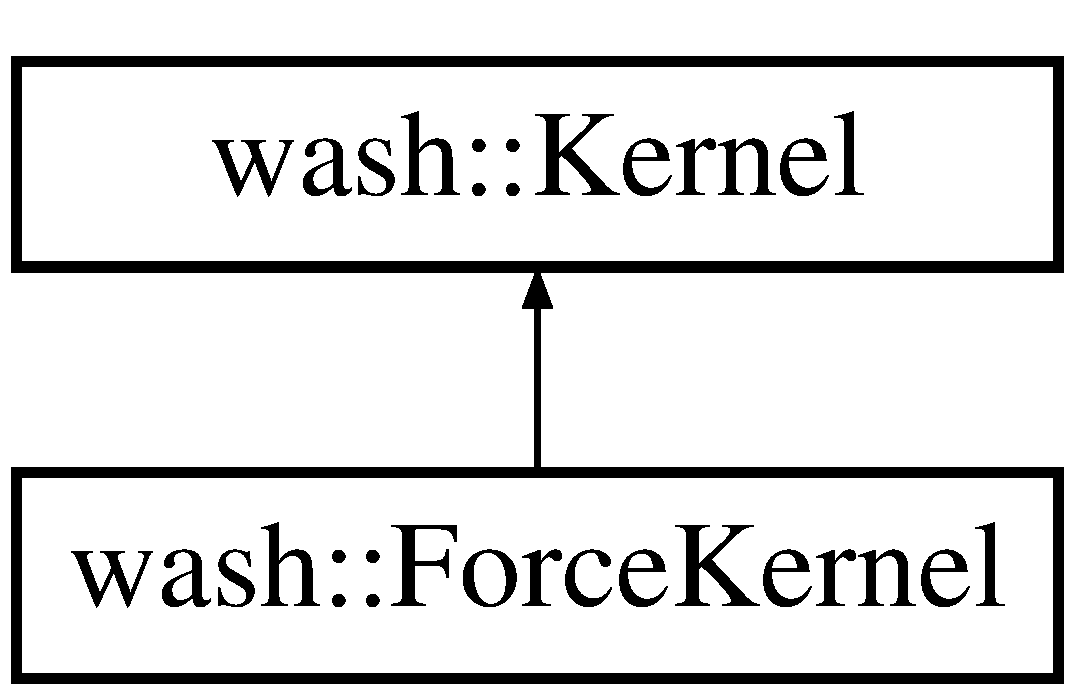
\includegraphics[height=2.000000cm]{classwash_1_1ForceKernel}
\end{center}
\end{figure}
\subsection*{Public Member Functions}
\begin{DoxyCompactItemize}
\item 
\mbox{\hyperlink{classwash_1_1ForceKernel_a5dd87d8036d74c210c51fb6aa97a3de8}{Force\+Kernel}} (const \mbox{\hyperlink{namespacewash_a3687ea698f8cb8c077d728e5d74de495}{Force\+FuncT}} func)
\item 
virtual void \mbox{\hyperlink{classwash_1_1ForceKernel_aa815514d4e9af5ebb056dbe8f1d5a720}{exec}} () const override
\end{DoxyCompactItemize}


\subsection{Detailed Description}
Force \mbox{\hyperlink{classwash_1_1Kernel}{Kernel}} Class. 

This kernel is used to update a force (or multiple forces) of a particle given its neighbours. 

\subsection{Constructor \& Destructor Documentation}
\mbox{\Hypertarget{classwash_1_1ForceKernel_a5dd87d8036d74c210c51fb6aa97a3de8}\label{classwash_1_1ForceKernel_a5dd87d8036d74c210c51fb6aa97a3de8}} 
\index{wash\+::\+Force\+Kernel@{wash\+::\+Force\+Kernel}!Force\+Kernel@{Force\+Kernel}}
\index{Force\+Kernel@{Force\+Kernel}!wash\+::\+Force\+Kernel@{wash\+::\+Force\+Kernel}}
\subsubsection{\texorpdfstring{Force\+Kernel()}{ForceKernel()}}
{\footnotesize\ttfamily wash\+::\+Force\+Kernel\+::\+Force\+Kernel (\begin{DoxyParamCaption}\item[{const \mbox{\hyperlink{namespacewash_a3687ea698f8cb8c077d728e5d74de495}{Force\+FuncT}}}]{func }\end{DoxyParamCaption})\hspace{0.3cm}{\ttfamily [inline]}}



\subsection{Member Function Documentation}
\mbox{\Hypertarget{classwash_1_1ForceKernel_aa815514d4e9af5ebb056dbe8f1d5a720}\label{classwash_1_1ForceKernel_aa815514d4e9af5ebb056dbe8f1d5a720}} 
\index{wash\+::\+Force\+Kernel@{wash\+::\+Force\+Kernel}!exec@{exec}}
\index{exec@{exec}!wash\+::\+Force\+Kernel@{wash\+::\+Force\+Kernel}}
\subsubsection{\texorpdfstring{exec()}{exec()}}
{\footnotesize\ttfamily void wash\+::\+Force\+Kernel\+::exec (\begin{DoxyParamCaption}{ }\end{DoxyParamCaption}) const\hspace{0.3cm}{\ttfamily [override]}, {\ttfamily [virtual]}}



Implements \mbox{\hyperlink{classwash_1_1Kernel_a0ec211840402ce975997b22136f16e39}{wash\+::\+Kernel}}.



The documentation for this class was generated from the following files\+:\begin{DoxyCompactItemize}
\item 
/dcs/20/u2002000/4th\+Year\+Project/wash/include/\mbox{\hyperlink{kernels_8hpp}{kernels.\+hpp}}\item 
/dcs/20/u2002000/4th\+Year\+Project/wash/src/impl/cstone/\mbox{\hyperlink{cstone_2kernels_8cpp}{kernels.\+cpp}}\end{DoxyCompactItemize}

\hypertarget{structImplementationFeatures}{}\section{Implementation\+Features Struct Reference}
\label{structImplementationFeatures}\index{Implementation\+Features@{Implementation\+Features}}


{\ttfamily \#include $<$common.\+hpp$>$}

\subsection*{Public Attributes}
\begin{DoxyCompactItemize}
\item 
uint8\+\_\+t \mbox{\hyperlink{structImplementationFeatures_a38b97cc0b2f3ea9db019845264fc060b}{openmp}}
\item 
uint8\+\_\+t \mbox{\hyperlink{structImplementationFeatures_a87a6ded1fc05396de42c11b17d41beca}{mpi}}
\item 
uint8\+\_\+t \mbox{\hyperlink{structImplementationFeatures_ac8156c774edb85175df22ff7f31dda44}{cuda}}
\item 
uint8\+\_\+t \mbox{\hyperlink{structImplementationFeatures_aaeaaaf6e801ac06863ba363591e938d7}{dim}}
\item 
std\+::string \mbox{\hyperlink{structImplementationFeatures_a7b7fb4c4e8fbf262d6697b8c25a17b5f}{name}}
\item 
std\+::string \mbox{\hyperlink{structImplementationFeatures_afe154ad26b28217f95c4cc74d7112049}{source\+\_\+dir}}
\end{DoxyCompactItemize}


\subsection{Member Data Documentation}
\mbox{\Hypertarget{structImplementationFeatures_ac8156c774edb85175df22ff7f31dda44}\label{structImplementationFeatures_ac8156c774edb85175df22ff7f31dda44}} 
\index{Implementation\+Features@{Implementation\+Features}!cuda@{cuda}}
\index{cuda@{cuda}!Implementation\+Features@{Implementation\+Features}}
\subsubsection{\texorpdfstring{cuda}{cuda}}
{\footnotesize\ttfamily uint8\+\_\+t Implementation\+Features\+::cuda}

\mbox{\Hypertarget{structImplementationFeatures_aaeaaaf6e801ac06863ba363591e938d7}\label{structImplementationFeatures_aaeaaaf6e801ac06863ba363591e938d7}} 
\index{Implementation\+Features@{Implementation\+Features}!dim@{dim}}
\index{dim@{dim}!Implementation\+Features@{Implementation\+Features}}
\subsubsection{\texorpdfstring{dim}{dim}}
{\footnotesize\ttfamily uint8\+\_\+t Implementation\+Features\+::dim}

\mbox{\Hypertarget{structImplementationFeatures_a87a6ded1fc05396de42c11b17d41beca}\label{structImplementationFeatures_a87a6ded1fc05396de42c11b17d41beca}} 
\index{Implementation\+Features@{Implementation\+Features}!mpi@{mpi}}
\index{mpi@{mpi}!Implementation\+Features@{Implementation\+Features}}
\subsubsection{\texorpdfstring{mpi}{mpi}}
{\footnotesize\ttfamily uint8\+\_\+t Implementation\+Features\+::mpi}

\mbox{\Hypertarget{structImplementationFeatures_a7b7fb4c4e8fbf262d6697b8c25a17b5f}\label{structImplementationFeatures_a7b7fb4c4e8fbf262d6697b8c25a17b5f}} 
\index{Implementation\+Features@{Implementation\+Features}!name@{name}}
\index{name@{name}!Implementation\+Features@{Implementation\+Features}}
\subsubsection{\texorpdfstring{name}{name}}
{\footnotesize\ttfamily std\+::string Implementation\+Features\+::name}

\mbox{\Hypertarget{structImplementationFeatures_a38b97cc0b2f3ea9db019845264fc060b}\label{structImplementationFeatures_a38b97cc0b2f3ea9db019845264fc060b}} 
\index{Implementation\+Features@{Implementation\+Features}!openmp@{openmp}}
\index{openmp@{openmp}!Implementation\+Features@{Implementation\+Features}}
\subsubsection{\texorpdfstring{openmp}{openmp}}
{\footnotesize\ttfamily uint8\+\_\+t Implementation\+Features\+::openmp}

\mbox{\Hypertarget{structImplementationFeatures_afe154ad26b28217f95c4cc74d7112049}\label{structImplementationFeatures_afe154ad26b28217f95c4cc74d7112049}} 
\index{Implementation\+Features@{Implementation\+Features}!source\+\_\+dir@{source\+\_\+dir}}
\index{source\+\_\+dir@{source\+\_\+dir}!Implementation\+Features@{Implementation\+Features}}
\subsubsection{\texorpdfstring{source\+\_\+dir}{source\_dir}}
{\footnotesize\ttfamily std\+::string Implementation\+Features\+::source\+\_\+dir}



The documentation for this struct was generated from the following file\+:\begin{DoxyCompactItemize}
\item 
/dcs/20/u2002000/4th\+Year\+Project/wash/src/ws2st/\mbox{\hyperlink{common_8hpp}{common.\+hpp}}\end{DoxyCompactItemize}

\hypertarget{classwash_1_1io_1_1IOManager}{}\section{wash\+:\+:io\+:\+:I\+O\+Manager Class Reference}
\label{classwash_1_1io_1_1IOManager}\index{wash\+::io\+::\+I\+O\+Manager@{wash\+::io\+::\+I\+O\+Manager}}


Manages the IO options for the simulation.  




{\ttfamily \#include $<$io.\+hpp$>$}

\subsection*{Public Types}
\begin{DoxyCompactItemize}
\item 
using \mbox{\hyperlink{classwash_1_1io_1_1IOManager_aeda8c39a8e3c748efd1b3e0f8ae823ee}{Writer\+FuncT}} = std\+::function$<$ int(const \mbox{\hyperlink{classwash_1_1io_1_1IOManager}{io\+::\+I\+O\+Manager}} \&, const \mbox{\hyperlink{structwash_1_1io_1_1SimulationData}{Simulation\+Data}} \&, const size\+\_\+t)$>$
\end{DoxyCompactItemize}
\subsection*{Public Member Functions}
\begin{DoxyCompactItemize}
\item 
\mbox{\hyperlink{classwash_1_1io_1_1IOManager_acea5f3f8a7f3e8eb1bfda9bc551b8435}{I\+O\+Manager}} (const std\+::string format, \mbox{\hyperlink{classwash_1_1io_1_1IOManager_aeda8c39a8e3c748efd1b3e0f8ae823ee}{Writer\+FuncT}} writer, const size\+\_\+t nth, const size\+\_\+t rank=0, const size\+\_\+t size=1, const bool \mbox{\hyperlink{namespacewash_a40aed5edcd0e0403841e3f83eaa41965}{timings}}=true)
\item 
\mbox{\hyperlink{classwash_1_1io_1_1IOManager_a736c595ca08833f2a4df8f0db90ceb28}{I\+O\+Manager}} (const std\+::string format, \mbox{\hyperlink{classwash_1_1io_1_1IOManager_aeda8c39a8e3c748efd1b3e0f8ae823ee}{Writer\+FuncT}} writer)
\item 
\mbox{\hyperlink{classwash_1_1io_1_1IOManager_af011701d8fed420a51bafe7fcf035774}{I\+O\+Manager}} (const std\+::string format, \mbox{\hyperlink{classwash_1_1io_1_1IOManager_aeda8c39a8e3c748efd1b3e0f8ae823ee}{Writer\+FuncT}} writer, const size\+\_\+t rank, const size\+\_\+t size)
\item 
\mbox{\hyperlink{classwash_1_1io_1_1IOManager_a2abea2ab5058a02b4bcf0876c0e179f7}{I\+O\+Manager}} ()
\item 
const std\+::string \mbox{\hyperlink{classwash_1_1io_1_1IOManager_aded7d1dbc7a4c2fc21e3a914ea0ea3b0}{get\+\_\+path}} () const
\item 
size\+\_\+t \mbox{\hyperlink{classwash_1_1io_1_1IOManager_ad290bc39e3c9ccafb070bf6ba75597b6}{get\+\_\+rank}} () const
\item 
size\+\_\+t \mbox{\hyperlink{classwash_1_1io_1_1IOManager_a01f3e40f12375f3128ad9b19f3ecda12}{get\+\_\+size}} () const
\item 
void \mbox{\hyperlink{classwash_1_1io_1_1IOManager_ab599141d728a1d6c09ce273a9e556eff}{set\+\_\+gather}} (bool value=true)
\item 
const std\+::string \& \mbox{\hyperlink{classwash_1_1io_1_1IOManager_ac0942e50fcd001ef853c8eb6b107e92d}{expand\+\_\+label}} (const std\+::string \&label) const
\begin{DoxyCompactList}\small\item\em Helper function to expand a label if an expansion exists. \end{DoxyCompactList}\item 
const \mbox{\hyperlink{structwash_1_1io_1_1SimulationData}{Simulation\+Data}} \mbox{\hyperlink{classwash_1_1io_1_1IOManager_acd4d5358ca4bb964926dfc080a72475c}{get\+\_\+simulation\+\_\+data}} ()
\begin{DoxyCompactList}\small\item\em Copies the simulation data at the current point of the simulation. \end{DoxyCompactList}\item 
void \mbox{\hyperlink{classwash_1_1io_1_1IOManager_ab4670696bfb277a364f6112fc6f0d051}{write\+\_\+iteration}} (const size\+\_\+t iteration)
\begin{DoxyCompactList}\small\item\em Dispatches an iteration call to the writer based on the iteration number. \end{DoxyCompactList}\item 
void \mbox{\hyperlink{classwash_1_1io_1_1IOManager_ab2397361f7dc4f7b54b559d332bafb11}{write\+\_\+timings}} (const std\+::string \&event\+\_\+name, const int tag, const int64\+\_\+t time\+\_\+taken) const
\begin{DoxyCompactList}\small\item\em Write a timing even out to a file. \end{DoxyCompactList}\item 
void \mbox{\hyperlink{classwash_1_1io_1_1IOManager_ae23d3d68354b0ba5b410992c60fe6762}{new\+\_\+timings}} ()
\begin{DoxyCompactList}\small\item\em Clear the timings output file. \end{DoxyCompactList}\end{DoxyCompactItemize}
\subsection*{Static Public Attributes}
\begin{DoxyCompactItemize}
\item 
static const std\+::unordered\+\_\+map$<$ std\+::string, std\+::string $>$ \mbox{\hyperlink{classwash_1_1io_1_1IOManager_ae2918fb006b6571b0eeceed90d2685b4}{label\+\_\+map}}
\end{DoxyCompactItemize}


\subsection{Detailed Description}
Manages the IO options for the simulation. 

\subsection{Member Typedef Documentation}
\mbox{\Hypertarget{classwash_1_1io_1_1IOManager_aeda8c39a8e3c748efd1b3e0f8ae823ee}\label{classwash_1_1io_1_1IOManager_aeda8c39a8e3c748efd1b3e0f8ae823ee}} 
\index{wash\+::io\+::\+I\+O\+Manager@{wash\+::io\+::\+I\+O\+Manager}!Writer\+FuncT@{Writer\+FuncT}}
\index{Writer\+FuncT@{Writer\+FuncT}!wash\+::io\+::\+I\+O\+Manager@{wash\+::io\+::\+I\+O\+Manager}}
\subsubsection{\texorpdfstring{Writer\+FuncT}{WriterFuncT}}
{\footnotesize\ttfamily using \mbox{\hyperlink{classwash_1_1io_1_1IOManager_aeda8c39a8e3c748efd1b3e0f8ae823ee}{wash\+::io\+::\+I\+O\+Manager\+::\+Writer\+FuncT}} =  std\+::function$<$int(const \mbox{\hyperlink{classwash_1_1io_1_1IOManager}{io\+::\+I\+O\+Manager}}\&, const \mbox{\hyperlink{structwash_1_1io_1_1SimulationData}{Simulation\+Data}}\&, const size\+\_\+t)$>$}



\subsection{Constructor \& Destructor Documentation}
\mbox{\Hypertarget{classwash_1_1io_1_1IOManager_acea5f3f8a7f3e8eb1bfda9bc551b8435}\label{classwash_1_1io_1_1IOManager_acea5f3f8a7f3e8eb1bfda9bc551b8435}} 
\index{wash\+::io\+::\+I\+O\+Manager@{wash\+::io\+::\+I\+O\+Manager}!I\+O\+Manager@{I\+O\+Manager}}
\index{I\+O\+Manager@{I\+O\+Manager}!wash\+::io\+::\+I\+O\+Manager@{wash\+::io\+::\+I\+O\+Manager}}
\subsubsection{\texorpdfstring{I\+O\+Manager()}{IOManager()}\hspace{0.1cm}{\footnotesize\ttfamily [1/4]}}
{\footnotesize\ttfamily wash\+::io\+::\+I\+O\+Manager\+::\+I\+O\+Manager (\begin{DoxyParamCaption}\item[{const std\+::string}]{format,  }\item[{\mbox{\hyperlink{classwash_1_1io_1_1IOManager_aeda8c39a8e3c748efd1b3e0f8ae823ee}{Writer\+FuncT}}}]{writer,  }\item[{const size\+\_\+t}]{nth,  }\item[{const size\+\_\+t}]{rank = {\ttfamily 0},  }\item[{const size\+\_\+t}]{size = {\ttfamily 1},  }\item[{const bool}]{timings = {\ttfamily true} }\end{DoxyParamCaption})\hspace{0.3cm}{\ttfamily [inline]}}

\mbox{\Hypertarget{classwash_1_1io_1_1IOManager_a736c595ca08833f2a4df8f0db90ceb28}\label{classwash_1_1io_1_1IOManager_a736c595ca08833f2a4df8f0db90ceb28}} 
\index{wash\+::io\+::\+I\+O\+Manager@{wash\+::io\+::\+I\+O\+Manager}!I\+O\+Manager@{I\+O\+Manager}}
\index{I\+O\+Manager@{I\+O\+Manager}!wash\+::io\+::\+I\+O\+Manager@{wash\+::io\+::\+I\+O\+Manager}}
\subsubsection{\texorpdfstring{I\+O\+Manager()}{IOManager()}\hspace{0.1cm}{\footnotesize\ttfamily [2/4]}}
{\footnotesize\ttfamily wash\+::io\+::\+I\+O\+Manager\+::\+I\+O\+Manager (\begin{DoxyParamCaption}\item[{const std\+::string}]{format,  }\item[{\mbox{\hyperlink{classwash_1_1io_1_1IOManager_aeda8c39a8e3c748efd1b3e0f8ae823ee}{Writer\+FuncT}}}]{writer }\end{DoxyParamCaption})\hspace{0.3cm}{\ttfamily [inline]}}

\mbox{\Hypertarget{classwash_1_1io_1_1IOManager_af011701d8fed420a51bafe7fcf035774}\label{classwash_1_1io_1_1IOManager_af011701d8fed420a51bafe7fcf035774}} 
\index{wash\+::io\+::\+I\+O\+Manager@{wash\+::io\+::\+I\+O\+Manager}!I\+O\+Manager@{I\+O\+Manager}}
\index{I\+O\+Manager@{I\+O\+Manager}!wash\+::io\+::\+I\+O\+Manager@{wash\+::io\+::\+I\+O\+Manager}}
\subsubsection{\texorpdfstring{I\+O\+Manager()}{IOManager()}\hspace{0.1cm}{\footnotesize\ttfamily [3/4]}}
{\footnotesize\ttfamily wash\+::io\+::\+I\+O\+Manager\+::\+I\+O\+Manager (\begin{DoxyParamCaption}\item[{const std\+::string}]{format,  }\item[{\mbox{\hyperlink{classwash_1_1io_1_1IOManager_aeda8c39a8e3c748efd1b3e0f8ae823ee}{Writer\+FuncT}}}]{writer,  }\item[{const size\+\_\+t}]{rank,  }\item[{const size\+\_\+t}]{size }\end{DoxyParamCaption})\hspace{0.3cm}{\ttfamily [inline]}}

\mbox{\Hypertarget{classwash_1_1io_1_1IOManager_a2abea2ab5058a02b4bcf0876c0e179f7}\label{classwash_1_1io_1_1IOManager_a2abea2ab5058a02b4bcf0876c0e179f7}} 
\index{wash\+::io\+::\+I\+O\+Manager@{wash\+::io\+::\+I\+O\+Manager}!I\+O\+Manager@{I\+O\+Manager}}
\index{I\+O\+Manager@{I\+O\+Manager}!wash\+::io\+::\+I\+O\+Manager@{wash\+::io\+::\+I\+O\+Manager}}
\subsubsection{\texorpdfstring{I\+O\+Manager()}{IOManager()}\hspace{0.1cm}{\footnotesize\ttfamily [4/4]}}
{\footnotesize\ttfamily wash\+::io\+::\+I\+O\+Manager\+::\+I\+O\+Manager (\begin{DoxyParamCaption}{ }\end{DoxyParamCaption})}



\subsection{Member Function Documentation}
\mbox{\Hypertarget{classwash_1_1io_1_1IOManager_ac0942e50fcd001ef853c8eb6b107e92d}\label{classwash_1_1io_1_1IOManager_ac0942e50fcd001ef853c8eb6b107e92d}} 
\index{wash\+::io\+::\+I\+O\+Manager@{wash\+::io\+::\+I\+O\+Manager}!expand\+\_\+label@{expand\+\_\+label}}
\index{expand\+\_\+label@{expand\+\_\+label}!wash\+::io\+::\+I\+O\+Manager@{wash\+::io\+::\+I\+O\+Manager}}
\subsubsection{\texorpdfstring{expand\+\_\+label()}{expand\_label()}}
{\footnotesize\ttfamily const std\+::string\& wash\+::io\+::\+I\+O\+Manager\+::expand\+\_\+label (\begin{DoxyParamCaption}\item[{const std\+::string \&}]{label }\end{DoxyParamCaption}) const\hspace{0.3cm}{\ttfamily [inline]}}



Helper function to expand a label if an expansion exists. 

\mbox{\Hypertarget{classwash_1_1io_1_1IOManager_aded7d1dbc7a4c2fc21e3a914ea0ea3b0}\label{classwash_1_1io_1_1IOManager_aded7d1dbc7a4c2fc21e3a914ea0ea3b0}} 
\index{wash\+::io\+::\+I\+O\+Manager@{wash\+::io\+::\+I\+O\+Manager}!get\+\_\+path@{get\+\_\+path}}
\index{get\+\_\+path@{get\+\_\+path}!wash\+::io\+::\+I\+O\+Manager@{wash\+::io\+::\+I\+O\+Manager}}
\subsubsection{\texorpdfstring{get\+\_\+path()}{get\_path()}}
{\footnotesize\ttfamily const std\+::string wash\+::io\+::\+I\+O\+Manager\+::get\+\_\+path (\begin{DoxyParamCaption}{ }\end{DoxyParamCaption}) const\hspace{0.3cm}{\ttfamily [inline]}}

\mbox{\Hypertarget{classwash_1_1io_1_1IOManager_ad290bc39e3c9ccafb070bf6ba75597b6}\label{classwash_1_1io_1_1IOManager_ad290bc39e3c9ccafb070bf6ba75597b6}} 
\index{wash\+::io\+::\+I\+O\+Manager@{wash\+::io\+::\+I\+O\+Manager}!get\+\_\+rank@{get\+\_\+rank}}
\index{get\+\_\+rank@{get\+\_\+rank}!wash\+::io\+::\+I\+O\+Manager@{wash\+::io\+::\+I\+O\+Manager}}
\subsubsection{\texorpdfstring{get\+\_\+rank()}{get\_rank()}}
{\footnotesize\ttfamily size\+\_\+t wash\+::io\+::\+I\+O\+Manager\+::get\+\_\+rank (\begin{DoxyParamCaption}{ }\end{DoxyParamCaption}) const\hspace{0.3cm}{\ttfamily [inline]}}

\mbox{\Hypertarget{classwash_1_1io_1_1IOManager_acd4d5358ca4bb964926dfc080a72475c}\label{classwash_1_1io_1_1IOManager_acd4d5358ca4bb964926dfc080a72475c}} 
\index{wash\+::io\+::\+I\+O\+Manager@{wash\+::io\+::\+I\+O\+Manager}!get\+\_\+simulation\+\_\+data@{get\+\_\+simulation\+\_\+data}}
\index{get\+\_\+simulation\+\_\+data@{get\+\_\+simulation\+\_\+data}!wash\+::io\+::\+I\+O\+Manager@{wash\+::io\+::\+I\+O\+Manager}}
\subsubsection{\texorpdfstring{get\+\_\+simulation\+\_\+data()}{get\_simulation\_data()}}
{\footnotesize\ttfamily const \mbox{\hyperlink{structwash_1_1io_1_1SimulationData}{Simulation\+Data}} wash\+::io\+::\+I\+O\+Manager\+::get\+\_\+simulation\+\_\+data (\begin{DoxyParamCaption}{ }\end{DoxyParamCaption})\hspace{0.3cm}{\ttfamily [inline]}}



Copies the simulation data at the current point of the simulation. 

If set to use a gather this will use M\+PI to gather from all processes

\begin{DoxyReturn}{Returns}
\mbox{\hyperlink{structwash_1_1io_1_1SimulationData}{Simulation\+Data}} The simulation data 
\end{DoxyReturn}
\mbox{\Hypertarget{classwash_1_1io_1_1IOManager_a01f3e40f12375f3128ad9b19f3ecda12}\label{classwash_1_1io_1_1IOManager_a01f3e40f12375f3128ad9b19f3ecda12}} 
\index{wash\+::io\+::\+I\+O\+Manager@{wash\+::io\+::\+I\+O\+Manager}!get\+\_\+size@{get\+\_\+size}}
\index{get\+\_\+size@{get\+\_\+size}!wash\+::io\+::\+I\+O\+Manager@{wash\+::io\+::\+I\+O\+Manager}}
\subsubsection{\texorpdfstring{get\+\_\+size()}{get\_size()}}
{\footnotesize\ttfamily size\+\_\+t wash\+::io\+::\+I\+O\+Manager\+::get\+\_\+size (\begin{DoxyParamCaption}{ }\end{DoxyParamCaption}) const\hspace{0.3cm}{\ttfamily [inline]}}

\mbox{\Hypertarget{classwash_1_1io_1_1IOManager_ae23d3d68354b0ba5b410992c60fe6762}\label{classwash_1_1io_1_1IOManager_ae23d3d68354b0ba5b410992c60fe6762}} 
\index{wash\+::io\+::\+I\+O\+Manager@{wash\+::io\+::\+I\+O\+Manager}!new\+\_\+timings@{new\+\_\+timings}}
\index{new\+\_\+timings@{new\+\_\+timings}!wash\+::io\+::\+I\+O\+Manager@{wash\+::io\+::\+I\+O\+Manager}}
\subsubsection{\texorpdfstring{new\+\_\+timings()}{new\_timings()}}
{\footnotesize\ttfamily void wash\+::io\+::\+I\+O\+Manager\+::new\+\_\+timings (\begin{DoxyParamCaption}{ }\end{DoxyParamCaption})\hspace{0.3cm}{\ttfamily [inline]}}



Clear the timings output file. 

\mbox{\Hypertarget{classwash_1_1io_1_1IOManager_ab599141d728a1d6c09ce273a9e556eff}\label{classwash_1_1io_1_1IOManager_ab599141d728a1d6c09ce273a9e556eff}} 
\index{wash\+::io\+::\+I\+O\+Manager@{wash\+::io\+::\+I\+O\+Manager}!set\+\_\+gather@{set\+\_\+gather}}
\index{set\+\_\+gather@{set\+\_\+gather}!wash\+::io\+::\+I\+O\+Manager@{wash\+::io\+::\+I\+O\+Manager}}
\subsubsection{\texorpdfstring{set\+\_\+gather()}{set\_gather()}}
{\footnotesize\ttfamily void wash\+::io\+::\+I\+O\+Manager\+::set\+\_\+gather (\begin{DoxyParamCaption}\item[{bool}]{value = {\ttfamily true} }\end{DoxyParamCaption})\hspace{0.3cm}{\ttfamily [inline]}}

\mbox{\Hypertarget{classwash_1_1io_1_1IOManager_ab4670696bfb277a364f6112fc6f0d051}\label{classwash_1_1io_1_1IOManager_ab4670696bfb277a364f6112fc6f0d051}} 
\index{wash\+::io\+::\+I\+O\+Manager@{wash\+::io\+::\+I\+O\+Manager}!write\+\_\+iteration@{write\+\_\+iteration}}
\index{write\+\_\+iteration@{write\+\_\+iteration}!wash\+::io\+::\+I\+O\+Manager@{wash\+::io\+::\+I\+O\+Manager}}
\subsubsection{\texorpdfstring{write\+\_\+iteration()}{write\_iteration()}}
{\footnotesize\ttfamily void wash\+::io\+::\+I\+O\+Manager\+::write\+\_\+iteration (\begin{DoxyParamCaption}\item[{const size\+\_\+t}]{iteration }\end{DoxyParamCaption})\hspace{0.3cm}{\ttfamily [inline]}}



Dispatches an iteration call to the writer based on the iteration number. 


\begin{DoxyParams}{Parameters}
{\em iteration} & \\
\hline
\end{DoxyParams}
\mbox{\Hypertarget{classwash_1_1io_1_1IOManager_ab2397361f7dc4f7b54b559d332bafb11}\label{classwash_1_1io_1_1IOManager_ab2397361f7dc4f7b54b559d332bafb11}} 
\index{wash\+::io\+::\+I\+O\+Manager@{wash\+::io\+::\+I\+O\+Manager}!write\+\_\+timings@{write\+\_\+timings}}
\index{write\+\_\+timings@{write\+\_\+timings}!wash\+::io\+::\+I\+O\+Manager@{wash\+::io\+::\+I\+O\+Manager}}
\subsubsection{\texorpdfstring{write\+\_\+timings()}{write\_timings()}}
{\footnotesize\ttfamily void wash\+::io\+::\+I\+O\+Manager\+::write\+\_\+timings (\begin{DoxyParamCaption}\item[{const std\+::string \&}]{event\+\_\+name,  }\item[{const int}]{tag,  }\item[{const int64\+\_\+t}]{time\+\_\+taken }\end{DoxyParamCaption}) const\hspace{0.3cm}{\ttfamily [inline]}}



Write a timing even out to a file. 


\begin{DoxyParams}{Parameters}
{\em event\+\_\+name} & \\
\hline
{\em time\+\_\+taken} & \\
\hline
\end{DoxyParams}


\subsection{Member Data Documentation}
\mbox{\Hypertarget{classwash_1_1io_1_1IOManager_ae2918fb006b6571b0eeceed90d2685b4}\label{classwash_1_1io_1_1IOManager_ae2918fb006b6571b0eeceed90d2685b4}} 
\index{wash\+::io\+::\+I\+O\+Manager@{wash\+::io\+::\+I\+O\+Manager}!label\+\_\+map@{label\+\_\+map}}
\index{label\+\_\+map@{label\+\_\+map}!wash\+::io\+::\+I\+O\+Manager@{wash\+::io\+::\+I\+O\+Manager}}
\subsubsection{\texorpdfstring{label\+\_\+map}{label\_map}}
{\footnotesize\ttfamily const std\+::unordered\+\_\+map$<$ std\+::string, std\+::string $>$ wash\+::io\+::\+I\+O\+Manager\+::label\+\_\+map\hspace{0.3cm}{\ttfamily [static]}}

{\bfseries Initial value\+:}
\begin{DoxyCode}
= \{ 
        \{\textcolor{stringliteral}{"id"}, \textcolor{stringliteral}{"ParticleIDs"}\},
        \{\textcolor{stringliteral}{"pos"}, \textcolor{stringliteral}{"Coordinates"}\},
        \{\textcolor{stringliteral}{"vel"}, \textcolor{stringliteral}{"Velocities"}\},
        \{\textcolor{stringliteral}{"acc"}, \textcolor{stringliteral}{"Acceleration"}\},
        \{\textcolor{stringliteral}{"rho"}, \textcolor{stringliteral}{"Density"}\},
        \{\textcolor{stringliteral}{"density"}, \textcolor{stringliteral}{"Density"}\},
        \{\textcolor{stringliteral}{"h"}, \textcolor{stringliteral}{"SmoothingLength"}\},
        \{\textcolor{stringliteral}{"smoothing\_length"}, \textcolor{stringliteral}{"SmoothingLength"}\},
        \{\textcolor{stringliteral}{"m"}, \textcolor{stringliteral}{"Masses"}\},
        \{\textcolor{stringliteral}{"mass"}, \textcolor{stringliteral}{"Masses"}\}
    \}
\end{DoxyCode}


The documentation for this class was generated from the following files\+:\begin{DoxyCompactItemize}
\item 
/dcs/20/u2002000/4th\+Year\+Project/wash/include/\mbox{\hyperlink{io_8hpp}{io.\+hpp}}\item 
/dcs/20/u2002000/4th\+Year\+Project/wash/src/io/\mbox{\hyperlink{io_2io_8cpp}{io.\+cpp}}\end{DoxyCompactItemize}

\hypertarget{classwash_1_1Kernel}{}\section{wash\+:\+:Kernel Class Reference}
\label{classwash_1_1Kernel}\index{wash\+::\+Kernel@{wash\+::\+Kernel}}


Parent \mbox{\hyperlink{classwash_1_1Kernel}{Kernel}} Class.  




{\ttfamily \#include $<$kernels.\+hpp$>$}

Inheritance diagram for wash\+:\+:Kernel\+:\begin{figure}[H]
\begin{center}
\leavevmode
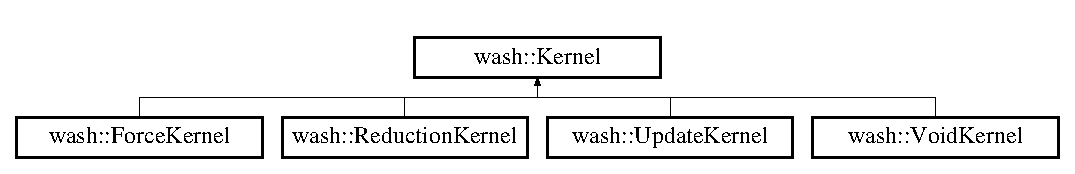
\includegraphics[height=1.891892cm]{classwash_1_1Kernel}
\end{center}
\end{figure}
\subsection*{Public Member Functions}
\begin{DoxyCompactItemize}
\item 
\mbox{\Hypertarget{classwash_1_1Kernel_a0ec211840402ce975997b22136f16e39}\label{classwash_1_1Kernel_a0ec211840402ce975997b22136f16e39}} 
virtual void {\bfseries exec} () const =0
\end{DoxyCompactItemize}


\subsection{Detailed Description}
Parent \mbox{\hyperlink{classwash_1_1Kernel}{Kernel}} Class. 

A \mbox{\hyperlink{classwash_1_1Kernel}{Kernel}} in Wa\+SH can take one of four forms, which all inherit from this class. 

The documentation for this class was generated from the following file\+:\begin{DoxyCompactItemize}
\item 
/dcs/20/u2002000/4th\+Year\+Project/wash/include/kernels.\+hpp\end{DoxyCompactItemize}

\hypertarget{structws2st_1_1KernelDependencies}{}\section{ws2st\+:\+:Kernel\+Dependencies Struct Reference}
\label{structws2st_1_1KernelDependencies}\index{ws2st\+::\+Kernel\+Dependencies@{ws2st\+::\+Kernel\+Dependencies}}


Struct to hold two vectors of dependencies (appropriately named)  




{\ttfamily \#include $<$common.\+hpp$>$}

\subsection*{Public Attributes}
\begin{DoxyCompactItemize}
\item 
\mbox{\Hypertarget{structws2st_1_1KernelDependencies_a4385ba2e56f0d9b63772480b2c3da15d}\label{structws2st_1_1KernelDependencies_a4385ba2e56f0d9b63772480b2c3da15d}} 
std\+::vector$<$ std\+::string $>$ {\bfseries reads\+\_\+from}
\item 
\mbox{\Hypertarget{structws2st_1_1KernelDependencies_a85a9ccadcb7d6912675a21cf500a4ef1}\label{structws2st_1_1KernelDependencies_a85a9ccadcb7d6912675a21cf500a4ef1}} 
std\+::vector$<$ std\+::string $>$ {\bfseries writes\+\_\+to}
\end{DoxyCompactItemize}


\subsection{Detailed Description}
Struct to hold two vectors of dependencies (appropriately named) 

The documentation for this struct was generated from the following file\+:\begin{DoxyCompactItemize}
\item 
/dcs/20/u2002000/4th\+Year\+Project/wash/src/ws2st/common.\+hpp\end{DoxyCompactItemize}

\hypertarget{classwash_1_1Particle}{}\section{wash\+:\+:Particle Class Reference}
\label{classwash_1_1Particle}\index{wash\+::\+Particle@{wash\+::\+Particle}}


{\ttfamily \#include $<$particle.\+hpp$>$}

\subsection*{Public Member Functions}
\begin{DoxyCompactItemize}
\item 
\mbox{\hyperlink{classwash_1_1Particle_a72131cdf3fdbcada383d81604fd49503}{Particle}} (const unsigned local\+\_\+idx)
\begin{DoxyCompactList}\small\item\em T\+O\+DO\+: see if this works if it\textquotesingle{}s a glocal spec defined flag rather than in just one file? \end{DoxyCompactList}\item 
unsigned \mbox{\hyperlink{classwash_1_1Particle_aef9f2814cc392598de7756e1046fea67}{get\+\_\+id}} () const
\begin{DoxyCompactList}\small\item\em Returns the global ID of the particle. \end{DoxyCompactList}\item 
double \mbox{\hyperlink{classwash_1_1Particle_a8c0ce3f48b189fd8550c3bfab17eec68}{get\+\_\+density}} () const
\item 
void \mbox{\hyperlink{classwash_1_1Particle_a6416678dd509c16c2933d315b6ae6156}{set\+\_\+density}} (const double \mbox{\hyperlink{3d__fluid__sim_2fluid__sim_8cpp_a140d94d7edb97c062961056d1926a2db}{density}})
\item 
double \mbox{\hyperlink{classwash_1_1Particle_a7d8d11b3e4855e66e62ee58b4270cdc1}{get\+\_\+mass}} () const
\item 
void \mbox{\hyperlink{classwash_1_1Particle_a9151ed34c880f63f062381076834223e}{set\+\_\+mass}} (const double mass)
\item 
double \mbox{\hyperlink{classwash_1_1Particle_aab02f56502c6521382cf7a7320abc341}{get\+\_\+smoothing\+\_\+length}} () const
\item 
void \mbox{\hyperlink{classwash_1_1Particle_a15892a4346c05de955f91087dc88786d}{set\+\_\+smoothing\+\_\+length}} (const double smoothing\+\_\+length)
\item 
\mbox{\hyperlink{namespacewash_ab2cbbc37941b733095c9225b49b4cad9}{Simulation\+VecT}} \mbox{\hyperlink{classwash_1_1Particle_a9d222d453d640cf629ee8dfbee6b43c2}{get\+\_\+pos}} () const
\item 
void \mbox{\hyperlink{classwash_1_1Particle_af06835533935c04e594c258a7dcdd1ef}{set\+\_\+pos}} (const \mbox{\hyperlink{namespacewash_ab2cbbc37941b733095c9225b49b4cad9}{Simulation\+VecT}} pos)
\item 
\mbox{\hyperlink{namespacewash_ab2cbbc37941b733095c9225b49b4cad9}{Simulation\+VecT}} \mbox{\hyperlink{classwash_1_1Particle_a890d0f1467225393e385872b0c98b974}{get\+\_\+vel}} () const
\item 
void \mbox{\hyperlink{classwash_1_1Particle_a4755365883cfd62117ebe74fe44d35e0}{set\+\_\+vel}} (const \mbox{\hyperlink{namespacewash_ab2cbbc37941b733095c9225b49b4cad9}{Simulation\+VecT}} vel)
\item 
\mbox{\hyperlink{namespacewash_ab2cbbc37941b733095c9225b49b4cad9}{Simulation\+VecT}} \mbox{\hyperlink{classwash_1_1Particle_afb8c9dce2692cdfab61a3a87fde50610}{get\+\_\+acc}} () const
\item 
void \mbox{\hyperlink{classwash_1_1Particle_a395e095de0b2af7dfc925bedef2090a1}{set\+\_\+acc}} (const \mbox{\hyperlink{namespacewash_ab2cbbc37941b733095c9225b49b4cad9}{Simulation\+VecT}} acc)
\item 
double \mbox{\hyperlink{classwash_1_1Particle_ab42a162b41a4e8cf6212bd9c43f3a0cf}{get\+\_\+force\+\_\+scalar}} (const std\+::string \&force) const
\item 
void \mbox{\hyperlink{classwash_1_1Particle_a2c3038c8eac34e371922bcf1ab79b8ca}{set\+\_\+force\+\_\+scalar}} (const std\+::string \&force, const double value)
\item 
\mbox{\hyperlink{namespacewash_ab2cbbc37941b733095c9225b49b4cad9}{Simulation\+VecT}} \mbox{\hyperlink{classwash_1_1Particle_a9c6ec5d5a7407897ecca00549bd05c01}{get\+\_\+force\+\_\+vector}} (const std\+::string \&force) const
\item 
void \mbox{\hyperlink{classwash_1_1Particle_a6960cdd169d1829a52e49cf835a8bfeb}{set\+\_\+force\+\_\+vector}} (const std\+::string \&force, const \mbox{\hyperlink{namespacewash_ab2cbbc37941b733095c9225b49b4cad9}{Simulation\+VecT}} value)
\item 
double \mbox{\hyperlink{classwash_1_1Particle_ab16021a2c003de07dc0a418ffc3d5eb7}{get\+\_\+vol}} () const
\item 
unsigned \mbox{\hyperlink{classwash_1_1Particle_a570fc3286ab83d081950a5fb3d548d92}{recalculate\+\_\+neighbors}} (unsigned max\+\_\+count) const
\item 
bool \mbox{\hyperlink{classwash_1_1Particle_a32369e6edba4277ebc71917a37c2503d}{operator==}} (const \mbox{\hyperlink{classwash_1_1Particle}{Particle}} \&other) const
\begin{DoxyCompactList}\small\item\em Compare particle equality by their I\+Ds. \end{DoxyCompactList}\item 
bool \mbox{\hyperlink{classwash_1_1Particle_a32f1334a8a0b273a57355956d7e9fe63}{operator!=}} (const \mbox{\hyperlink{classwash_1_1Particle}{Particle}} \&other) const
\begin{DoxyCompactList}\small\item\em Inverse of equality check. \end{DoxyCompactList}\item 
\mbox{\hyperlink{classwash_1_1Particle_a9ca04366cb7412e6aa5d1d89108a8520}{Particle}} (const \mbox{\hyperlink{classwash_1_1Particle}{Particle}} \&)=delete
\item 
\mbox{\hyperlink{classwash_1_1Particle}{Particle}} \& \mbox{\hyperlink{classwash_1_1Particle_a8ac44cec043e444a45ab189f666f9d4b}{operator=}} (const \mbox{\hyperlink{classwash_1_1Particle}{Particle}} \&)=delete
\end{DoxyCompactItemize}
\subsection*{Friends}
\begin{DoxyCompactItemize}
\item 
std\+::ostream \& \mbox{\hyperlink{classwash_1_1Particle_ad7d60c63b6d14d1d0d4fe42d4e9dc8bc}{operator$<$$<$}} (std\+::ostream \&os, const \mbox{\hyperlink{classwash_1_1Particle}{Particle}} \&p)
\end{DoxyCompactItemize}


\subsection{Constructor \& Destructor Documentation}
\mbox{\Hypertarget{classwash_1_1Particle_a72131cdf3fdbcada383d81604fd49503}\label{classwash_1_1Particle_a72131cdf3fdbcada383d81604fd49503}} 
\index{wash\+::\+Particle@{wash\+::\+Particle}!Particle@{Particle}}
\index{Particle@{Particle}!wash\+::\+Particle@{wash\+::\+Particle}}
\subsubsection{\texorpdfstring{Particle()}{Particle()}\hspace{0.1cm}{\footnotesize\ttfamily [1/2]}}
{\footnotesize\ttfamily wash\+::\+Particle\+::\+Particle (\begin{DoxyParamCaption}\item[{const unsigned}]{local\+\_\+idx }\end{DoxyParamCaption})}



T\+O\+DO\+: see if this works if it\textquotesingle{}s a glocal spec defined flag rather than in just one file? 

\mbox{\Hypertarget{classwash_1_1Particle_a9ca04366cb7412e6aa5d1d89108a8520}\label{classwash_1_1Particle_a9ca04366cb7412e6aa5d1d89108a8520}} 
\index{wash\+::\+Particle@{wash\+::\+Particle}!Particle@{Particle}}
\index{Particle@{Particle}!wash\+::\+Particle@{wash\+::\+Particle}}
\subsubsection{\texorpdfstring{Particle()}{Particle()}\hspace{0.1cm}{\footnotesize\ttfamily [2/2]}}
{\footnotesize\ttfamily wash\+::\+Particle\+::\+Particle (\begin{DoxyParamCaption}\item[{const \mbox{\hyperlink{classwash_1_1Particle}{Particle}} \&}]{ }\end{DoxyParamCaption})\hspace{0.3cm}{\ttfamily [delete]}}



\subsection{Member Function Documentation}
\mbox{\Hypertarget{classwash_1_1Particle_afb8c9dce2692cdfab61a3a87fde50610}\label{classwash_1_1Particle_afb8c9dce2692cdfab61a3a87fde50610}} 
\index{wash\+::\+Particle@{wash\+::\+Particle}!get\+\_\+acc@{get\+\_\+acc}}
\index{get\+\_\+acc@{get\+\_\+acc}!wash\+::\+Particle@{wash\+::\+Particle}}
\subsubsection{\texorpdfstring{get\+\_\+acc()}{get\_acc()}}
{\footnotesize\ttfamily \mbox{\hyperlink{namespacewash_ab2cbbc37941b733095c9225b49b4cad9}{Simulation\+VecT}} wash\+::\+Particle\+::get\+\_\+acc (\begin{DoxyParamCaption}{ }\end{DoxyParamCaption}) const}

\mbox{\Hypertarget{classwash_1_1Particle_a8c0ce3f48b189fd8550c3bfab17eec68}\label{classwash_1_1Particle_a8c0ce3f48b189fd8550c3bfab17eec68}} 
\index{wash\+::\+Particle@{wash\+::\+Particle}!get\+\_\+density@{get\+\_\+density}}
\index{get\+\_\+density@{get\+\_\+density}!wash\+::\+Particle@{wash\+::\+Particle}}
\subsubsection{\texorpdfstring{get\+\_\+density()}{get\_density()}}
{\footnotesize\ttfamily double wash\+::\+Particle\+::get\+\_\+density (\begin{DoxyParamCaption}{ }\end{DoxyParamCaption}) const}

\mbox{\Hypertarget{classwash_1_1Particle_ab42a162b41a4e8cf6212bd9c43f3a0cf}\label{classwash_1_1Particle_ab42a162b41a4e8cf6212bd9c43f3a0cf}} 
\index{wash\+::\+Particle@{wash\+::\+Particle}!get\+\_\+force\+\_\+scalar@{get\+\_\+force\+\_\+scalar}}
\index{get\+\_\+force\+\_\+scalar@{get\+\_\+force\+\_\+scalar}!wash\+::\+Particle@{wash\+::\+Particle}}
\subsubsection{\texorpdfstring{get\+\_\+force\+\_\+scalar()}{get\_force\_scalar()}}
{\footnotesize\ttfamily double wash\+::\+Particle\+::get\+\_\+force\+\_\+scalar (\begin{DoxyParamCaption}\item[{const std\+::string \&}]{force }\end{DoxyParamCaption}) const}

\mbox{\Hypertarget{classwash_1_1Particle_a9c6ec5d5a7407897ecca00549bd05c01}\label{classwash_1_1Particle_a9c6ec5d5a7407897ecca00549bd05c01}} 
\index{wash\+::\+Particle@{wash\+::\+Particle}!get\+\_\+force\+\_\+vector@{get\+\_\+force\+\_\+vector}}
\index{get\+\_\+force\+\_\+vector@{get\+\_\+force\+\_\+vector}!wash\+::\+Particle@{wash\+::\+Particle}}
\subsubsection{\texorpdfstring{get\+\_\+force\+\_\+vector()}{get\_force\_vector()}}
{\footnotesize\ttfamily \mbox{\hyperlink{namespacewash_ab2cbbc37941b733095c9225b49b4cad9}{Simulation\+VecT}} wash\+::\+Particle\+::get\+\_\+force\+\_\+vector (\begin{DoxyParamCaption}\item[{const std\+::string \&}]{force }\end{DoxyParamCaption}) const}

\mbox{\Hypertarget{classwash_1_1Particle_aef9f2814cc392598de7756e1046fea67}\label{classwash_1_1Particle_aef9f2814cc392598de7756e1046fea67}} 
\index{wash\+::\+Particle@{wash\+::\+Particle}!get\+\_\+id@{get\+\_\+id}}
\index{get\+\_\+id@{get\+\_\+id}!wash\+::\+Particle@{wash\+::\+Particle}}
\subsubsection{\texorpdfstring{get\+\_\+id()}{get\_id()}}
{\footnotesize\ttfamily unsigned wash\+::\+Particle\+::get\+\_\+id (\begin{DoxyParamCaption}{ }\end{DoxyParamCaption}) const}



Returns the global ID of the particle. 

\mbox{\Hypertarget{classwash_1_1Particle_a7d8d11b3e4855e66e62ee58b4270cdc1}\label{classwash_1_1Particle_a7d8d11b3e4855e66e62ee58b4270cdc1}} 
\index{wash\+::\+Particle@{wash\+::\+Particle}!get\+\_\+mass@{get\+\_\+mass}}
\index{get\+\_\+mass@{get\+\_\+mass}!wash\+::\+Particle@{wash\+::\+Particle}}
\subsubsection{\texorpdfstring{get\+\_\+mass()}{get\_mass()}}
{\footnotesize\ttfamily double wash\+::\+Particle\+::get\+\_\+mass (\begin{DoxyParamCaption}{ }\end{DoxyParamCaption}) const}

\mbox{\Hypertarget{classwash_1_1Particle_a9d222d453d640cf629ee8dfbee6b43c2}\label{classwash_1_1Particle_a9d222d453d640cf629ee8dfbee6b43c2}} 
\index{wash\+::\+Particle@{wash\+::\+Particle}!get\+\_\+pos@{get\+\_\+pos}}
\index{get\+\_\+pos@{get\+\_\+pos}!wash\+::\+Particle@{wash\+::\+Particle}}
\subsubsection{\texorpdfstring{get\+\_\+pos()}{get\_pos()}}
{\footnotesize\ttfamily \mbox{\hyperlink{namespacewash_ab2cbbc37941b733095c9225b49b4cad9}{Simulation\+VecT}} wash\+::\+Particle\+::get\+\_\+pos (\begin{DoxyParamCaption}{ }\end{DoxyParamCaption}) const}

\mbox{\Hypertarget{classwash_1_1Particle_aab02f56502c6521382cf7a7320abc341}\label{classwash_1_1Particle_aab02f56502c6521382cf7a7320abc341}} 
\index{wash\+::\+Particle@{wash\+::\+Particle}!get\+\_\+smoothing\+\_\+length@{get\+\_\+smoothing\+\_\+length}}
\index{get\+\_\+smoothing\+\_\+length@{get\+\_\+smoothing\+\_\+length}!wash\+::\+Particle@{wash\+::\+Particle}}
\subsubsection{\texorpdfstring{get\+\_\+smoothing\+\_\+length()}{get\_smoothing\_length()}}
{\footnotesize\ttfamily double wash\+::\+Particle\+::get\+\_\+smoothing\+\_\+length (\begin{DoxyParamCaption}{ }\end{DoxyParamCaption}) const}

\mbox{\Hypertarget{classwash_1_1Particle_a890d0f1467225393e385872b0c98b974}\label{classwash_1_1Particle_a890d0f1467225393e385872b0c98b974}} 
\index{wash\+::\+Particle@{wash\+::\+Particle}!get\+\_\+vel@{get\+\_\+vel}}
\index{get\+\_\+vel@{get\+\_\+vel}!wash\+::\+Particle@{wash\+::\+Particle}}
\subsubsection{\texorpdfstring{get\+\_\+vel()}{get\_vel()}}
{\footnotesize\ttfamily \mbox{\hyperlink{namespacewash_ab2cbbc37941b733095c9225b49b4cad9}{Simulation\+VecT}} wash\+::\+Particle\+::get\+\_\+vel (\begin{DoxyParamCaption}{ }\end{DoxyParamCaption}) const}

\mbox{\Hypertarget{classwash_1_1Particle_ab16021a2c003de07dc0a418ffc3d5eb7}\label{classwash_1_1Particle_ab16021a2c003de07dc0a418ffc3d5eb7}} 
\index{wash\+::\+Particle@{wash\+::\+Particle}!get\+\_\+vol@{get\+\_\+vol}}
\index{get\+\_\+vol@{get\+\_\+vol}!wash\+::\+Particle@{wash\+::\+Particle}}
\subsubsection{\texorpdfstring{get\+\_\+vol()}{get\_vol()}}
{\footnotesize\ttfamily double wash\+::\+Particle\+::get\+\_\+vol (\begin{DoxyParamCaption}{ }\end{DoxyParamCaption}) const}

\mbox{\Hypertarget{classwash_1_1Particle_a32f1334a8a0b273a57355956d7e9fe63}\label{classwash_1_1Particle_a32f1334a8a0b273a57355956d7e9fe63}} 
\index{wash\+::\+Particle@{wash\+::\+Particle}!operator"!=@{operator"!=}}
\index{operator"!=@{operator"!=}!wash\+::\+Particle@{wash\+::\+Particle}}
\subsubsection{\texorpdfstring{operator"!=()}{operator!=()}}
{\footnotesize\ttfamily bool wash\+::\+Particle\+::operator!= (\begin{DoxyParamCaption}\item[{const \mbox{\hyperlink{classwash_1_1Particle}{Particle}} \&}]{other }\end{DoxyParamCaption}) const}



Inverse of equality check. 


\begin{DoxyParams}{Parameters}
{\em other} & \\
\hline
\end{DoxyParams}
\begin{DoxyReturn}{Returns}
true 

false 
\end{DoxyReturn}
\mbox{\Hypertarget{classwash_1_1Particle_a8ac44cec043e444a45ab189f666f9d4b}\label{classwash_1_1Particle_a8ac44cec043e444a45ab189f666f9d4b}} 
\index{wash\+::\+Particle@{wash\+::\+Particle}!operator=@{operator=}}
\index{operator=@{operator=}!wash\+::\+Particle@{wash\+::\+Particle}}
\subsubsection{\texorpdfstring{operator=()}{operator=()}}
{\footnotesize\ttfamily \mbox{\hyperlink{classwash_1_1Particle}{Particle}}\& wash\+::\+Particle\+::operator= (\begin{DoxyParamCaption}\item[{const \mbox{\hyperlink{classwash_1_1Particle}{Particle}} \&}]{ }\end{DoxyParamCaption})\hspace{0.3cm}{\ttfamily [delete]}}

\mbox{\Hypertarget{classwash_1_1Particle_a32369e6edba4277ebc71917a37c2503d}\label{classwash_1_1Particle_a32369e6edba4277ebc71917a37c2503d}} 
\index{wash\+::\+Particle@{wash\+::\+Particle}!operator==@{operator==}}
\index{operator==@{operator==}!wash\+::\+Particle@{wash\+::\+Particle}}
\subsubsection{\texorpdfstring{operator==()}{operator==()}}
{\footnotesize\ttfamily bool wash\+::\+Particle\+::operator== (\begin{DoxyParamCaption}\item[{const \mbox{\hyperlink{classwash_1_1Particle}{Particle}} \&}]{other }\end{DoxyParamCaption}) const}



Compare particle equality by their I\+Ds. 


\begin{DoxyParams}{Parameters}
{\em other} & \\
\hline
\end{DoxyParams}
\begin{DoxyReturn}{Returns}
true ID\textquotesingle{}s equal 

false ID\textquotesingle{}s not equal 
\end{DoxyReturn}
\mbox{\Hypertarget{classwash_1_1Particle_a570fc3286ab83d081950a5fb3d548d92}\label{classwash_1_1Particle_a570fc3286ab83d081950a5fb3d548d92}} 
\index{wash\+::\+Particle@{wash\+::\+Particle}!recalculate\+\_\+neighbors@{recalculate\+\_\+neighbors}}
\index{recalculate\+\_\+neighbors@{recalculate\+\_\+neighbors}!wash\+::\+Particle@{wash\+::\+Particle}}
\subsubsection{\texorpdfstring{recalculate\+\_\+neighbors()}{recalculate\_neighbors()}}
{\footnotesize\ttfamily unsigned wash\+::\+Particle\+::recalculate\+\_\+neighbors (\begin{DoxyParamCaption}\item[{unsigned}]{max\+\_\+count }\end{DoxyParamCaption}) const}

\mbox{\Hypertarget{classwash_1_1Particle_a395e095de0b2af7dfc925bedef2090a1}\label{classwash_1_1Particle_a395e095de0b2af7dfc925bedef2090a1}} 
\index{wash\+::\+Particle@{wash\+::\+Particle}!set\+\_\+acc@{set\+\_\+acc}}
\index{set\+\_\+acc@{set\+\_\+acc}!wash\+::\+Particle@{wash\+::\+Particle}}
\subsubsection{\texorpdfstring{set\+\_\+acc()}{set\_acc()}}
{\footnotesize\ttfamily void wash\+::\+Particle\+::set\+\_\+acc (\begin{DoxyParamCaption}\item[{const \mbox{\hyperlink{namespacewash_ab2cbbc37941b733095c9225b49b4cad9}{Simulation\+VecT}}}]{acc }\end{DoxyParamCaption})}

\mbox{\Hypertarget{classwash_1_1Particle_a6416678dd509c16c2933d315b6ae6156}\label{classwash_1_1Particle_a6416678dd509c16c2933d315b6ae6156}} 
\index{wash\+::\+Particle@{wash\+::\+Particle}!set\+\_\+density@{set\+\_\+density}}
\index{set\+\_\+density@{set\+\_\+density}!wash\+::\+Particle@{wash\+::\+Particle}}
\subsubsection{\texorpdfstring{set\+\_\+density()}{set\_density()}}
{\footnotesize\ttfamily void wash\+::\+Particle\+::set\+\_\+density (\begin{DoxyParamCaption}\item[{const double}]{density }\end{DoxyParamCaption})}

\mbox{\Hypertarget{classwash_1_1Particle_a2c3038c8eac34e371922bcf1ab79b8ca}\label{classwash_1_1Particle_a2c3038c8eac34e371922bcf1ab79b8ca}} 
\index{wash\+::\+Particle@{wash\+::\+Particle}!set\+\_\+force\+\_\+scalar@{set\+\_\+force\+\_\+scalar}}
\index{set\+\_\+force\+\_\+scalar@{set\+\_\+force\+\_\+scalar}!wash\+::\+Particle@{wash\+::\+Particle}}
\subsubsection{\texorpdfstring{set\+\_\+force\+\_\+scalar()}{set\_force\_scalar()}}
{\footnotesize\ttfamily void wash\+::\+Particle\+::set\+\_\+force\+\_\+scalar (\begin{DoxyParamCaption}\item[{const std\+::string \&}]{force,  }\item[{const double}]{value }\end{DoxyParamCaption})}

\mbox{\Hypertarget{classwash_1_1Particle_a6960cdd169d1829a52e49cf835a8bfeb}\label{classwash_1_1Particle_a6960cdd169d1829a52e49cf835a8bfeb}} 
\index{wash\+::\+Particle@{wash\+::\+Particle}!set\+\_\+force\+\_\+vector@{set\+\_\+force\+\_\+vector}}
\index{set\+\_\+force\+\_\+vector@{set\+\_\+force\+\_\+vector}!wash\+::\+Particle@{wash\+::\+Particle}}
\subsubsection{\texorpdfstring{set\+\_\+force\+\_\+vector()}{set\_force\_vector()}}
{\footnotesize\ttfamily void wash\+::\+Particle\+::set\+\_\+force\+\_\+vector (\begin{DoxyParamCaption}\item[{const std\+::string \&}]{force,  }\item[{const \mbox{\hyperlink{namespacewash_ab2cbbc37941b733095c9225b49b4cad9}{Simulation\+VecT}}}]{value }\end{DoxyParamCaption})}

\mbox{\Hypertarget{classwash_1_1Particle_a9151ed34c880f63f062381076834223e}\label{classwash_1_1Particle_a9151ed34c880f63f062381076834223e}} 
\index{wash\+::\+Particle@{wash\+::\+Particle}!set\+\_\+mass@{set\+\_\+mass}}
\index{set\+\_\+mass@{set\+\_\+mass}!wash\+::\+Particle@{wash\+::\+Particle}}
\subsubsection{\texorpdfstring{set\+\_\+mass()}{set\_mass()}}
{\footnotesize\ttfamily void wash\+::\+Particle\+::set\+\_\+mass (\begin{DoxyParamCaption}\item[{const double}]{mass }\end{DoxyParamCaption})}

\mbox{\Hypertarget{classwash_1_1Particle_af06835533935c04e594c258a7dcdd1ef}\label{classwash_1_1Particle_af06835533935c04e594c258a7dcdd1ef}} 
\index{wash\+::\+Particle@{wash\+::\+Particle}!set\+\_\+pos@{set\+\_\+pos}}
\index{set\+\_\+pos@{set\+\_\+pos}!wash\+::\+Particle@{wash\+::\+Particle}}
\subsubsection{\texorpdfstring{set\+\_\+pos()}{set\_pos()}}
{\footnotesize\ttfamily void wash\+::\+Particle\+::set\+\_\+pos (\begin{DoxyParamCaption}\item[{const \mbox{\hyperlink{namespacewash_ab2cbbc37941b733095c9225b49b4cad9}{Simulation\+VecT}}}]{pos }\end{DoxyParamCaption})}

\mbox{\Hypertarget{classwash_1_1Particle_a15892a4346c05de955f91087dc88786d}\label{classwash_1_1Particle_a15892a4346c05de955f91087dc88786d}} 
\index{wash\+::\+Particle@{wash\+::\+Particle}!set\+\_\+smoothing\+\_\+length@{set\+\_\+smoothing\+\_\+length}}
\index{set\+\_\+smoothing\+\_\+length@{set\+\_\+smoothing\+\_\+length}!wash\+::\+Particle@{wash\+::\+Particle}}
\subsubsection{\texorpdfstring{set\+\_\+smoothing\+\_\+length()}{set\_smoothing\_length()}}
{\footnotesize\ttfamily void wash\+::\+Particle\+::set\+\_\+smoothing\+\_\+length (\begin{DoxyParamCaption}\item[{const double}]{smoothing\+\_\+length }\end{DoxyParamCaption})}

\mbox{\Hypertarget{classwash_1_1Particle_a4755365883cfd62117ebe74fe44d35e0}\label{classwash_1_1Particle_a4755365883cfd62117ebe74fe44d35e0}} 
\index{wash\+::\+Particle@{wash\+::\+Particle}!set\+\_\+vel@{set\+\_\+vel}}
\index{set\+\_\+vel@{set\+\_\+vel}!wash\+::\+Particle@{wash\+::\+Particle}}
\subsubsection{\texorpdfstring{set\+\_\+vel()}{set\_vel()}}
{\footnotesize\ttfamily void wash\+::\+Particle\+::set\+\_\+vel (\begin{DoxyParamCaption}\item[{const \mbox{\hyperlink{namespacewash_ab2cbbc37941b733095c9225b49b4cad9}{Simulation\+VecT}}}]{vel }\end{DoxyParamCaption})}



\subsection{Friends And Related Function Documentation}
\mbox{\Hypertarget{classwash_1_1Particle_ad7d60c63b6d14d1d0d4fe42d4e9dc8bc}\label{classwash_1_1Particle_ad7d60c63b6d14d1d0d4fe42d4e9dc8bc}} 
\index{wash\+::\+Particle@{wash\+::\+Particle}!operator$<$$<$@{operator$<$$<$}}
\index{operator$<$$<$@{operator$<$$<$}!wash\+::\+Particle@{wash\+::\+Particle}}
\subsubsection{\texorpdfstring{operator$<$$<$}{operator<<}}
{\footnotesize\ttfamily std\+::ostream\& operator$<$$<$ (\begin{DoxyParamCaption}\item[{std\+::ostream \&}]{os,  }\item[{const \mbox{\hyperlink{classwash_1_1Particle}{Particle}} \&}]{p }\end{DoxyParamCaption})\hspace{0.3cm}{\ttfamily [friend]}}



The documentation for this class was generated from the following files\+:\begin{DoxyCompactItemize}
\item 
/dcs/20/u2002000/4th\+Year\+Project/wash/include/\mbox{\hyperlink{particle_8hpp}{particle.\+hpp}}\item 
/dcs/20/u2002000/4th\+Year\+Project/wash/src/impl/cstone/\mbox{\hyperlink{cstone_2particle_8cpp}{particle.\+cpp}}\end{DoxyCompactItemize}

\hypertarget{classwash_1_1ReductionKernel}{}\section{wash\+:\+:Reduction\+Kernel Class Reference}
\label{classwash_1_1ReductionKernel}\index{wash\+::\+Reduction\+Kernel@{wash\+::\+Reduction\+Kernel}}
Inheritance diagram for wash\+:\+:Reduction\+Kernel\+:\begin{figure}[H]
\begin{center}
\leavevmode
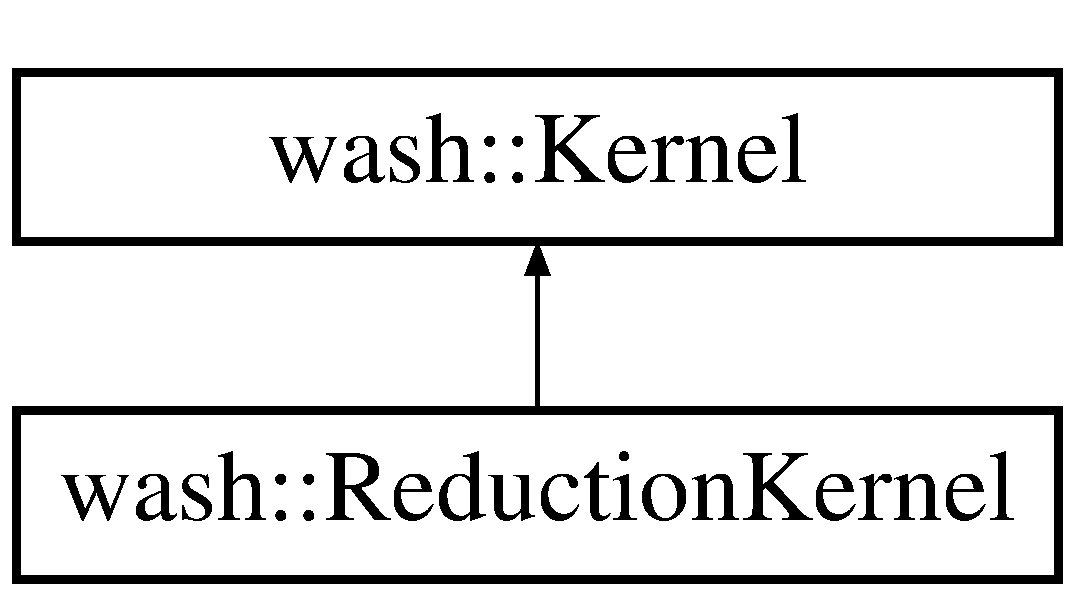
\includegraphics[height=2.000000cm]{classwash_1_1ReductionKernel}
\end{center}
\end{figure}
\subsection*{Public Member Functions}
\begin{DoxyCompactItemize}
\item 
\mbox{\Hypertarget{classwash_1_1ReductionKernel_ab916c2db7332203aed95dbd1adfbdd8e}\label{classwash_1_1ReductionKernel_ab916c2db7332203aed95dbd1adfbdd8e}} 
{\bfseries Reduction\+Kernel} (const Map\+FuncT map\+\_\+func, const Reduce\+FuncT reduce\+\_\+func, const double seed, const std\+::string variable)
\item 
\mbox{\Hypertarget{classwash_1_1ReductionKernel_a3ead90df8748700f40b2e6820e8e7e91}\label{classwash_1_1ReductionKernel_a3ead90df8748700f40b2e6820e8e7e91}} 
virtual void {\bfseries exec} () const override
\item 
\mbox{\Hypertarget{classwash_1_1ReductionKernel_ab916c2db7332203aed95dbd1adfbdd8e}\label{classwash_1_1ReductionKernel_ab916c2db7332203aed95dbd1adfbdd8e}} 
{\bfseries Reduction\+Kernel} (const Map\+FuncT map\+\_\+func, const Reduce\+FuncT reduce\+\_\+func, const double seed, const std\+::string variable)
\item 
\mbox{\Hypertarget{classwash_1_1ReductionKernel_aa06e992c0bc5d3e97fdf7553ad583bf3}\label{classwash_1_1ReductionKernel_aa06e992c0bc5d3e97fdf7553ad583bf3}} 
virtual void {\bfseries exec} () const override
\end{DoxyCompactItemize}


The documentation for this class was generated from the following files\+:\begin{DoxyCompactItemize}
\item 
/dcs/20/u2002000/4th\+Year\+Project/wash/src/wash/wash.\+hpp\item 
/dcs/20/u2002000/4th\+Year\+Project/wash/src/wash/wash.\+cpp\end{DoxyCompactItemize}

\hypertarget{classws2st_1_1refactor_1_1RefactoringToolConfiguration}{}\section{ws2st\+:\+:refactor\+:\+:Refactoring\+Tool\+Configuration Class Reference}
\label{classws2st_1_1refactor_1_1RefactoringToolConfiguration}\index{ws2st\+::refactor\+::\+Refactoring\+Tool\+Configuration@{ws2st\+::refactor\+::\+Refactoring\+Tool\+Configuration}}


We configure the whole tool by a series of refactoring passes.  




{\ttfamily \#include $<$refactor.\+hpp$>$}

\subsection*{Public Member Functions}
\begin{DoxyCompactItemize}
\item 
\mbox{\hyperlink{classws2st_1_1refactor_1_1RefactoringToolConfiguration_a6170e537d63c130d1224af83a5d0f41f}{Refactoring\+Tool\+Configuration}} (std\+::initializer\+\_\+list$<$ \mbox{\hyperlink{classws2st_1_1refactor_1_1RefactorPass}{Refactor\+Pass}} $>$ passes)
\item 
bool \mbox{\hyperlink{classws2st_1_1refactor_1_1RefactoringToolConfiguration_a7ff018cf2d0f2ec54274efcfa00df72f}{run}} (const \mbox{\hyperlink{structWashOptions}{Wash\+Options}} \&opts) const
\end{DoxyCompactItemize}


\subsection{Detailed Description}
We configure the whole tool by a series of refactoring passes. 


\begin{DoxyItemize}
\item each pass a stage where the tool runs through the source once 
\end{DoxyItemize}

\subsection{Constructor \& Destructor Documentation}
\mbox{\Hypertarget{classws2st_1_1refactor_1_1RefactoringToolConfiguration_a6170e537d63c130d1224af83a5d0f41f}\label{classws2st_1_1refactor_1_1RefactoringToolConfiguration_a6170e537d63c130d1224af83a5d0f41f}} 
\index{ws2st\+::refactor\+::\+Refactoring\+Tool\+Configuration@{ws2st\+::refactor\+::\+Refactoring\+Tool\+Configuration}!Refactoring\+Tool\+Configuration@{Refactoring\+Tool\+Configuration}}
\index{Refactoring\+Tool\+Configuration@{Refactoring\+Tool\+Configuration}!ws2st\+::refactor\+::\+Refactoring\+Tool\+Configuration@{ws2st\+::refactor\+::\+Refactoring\+Tool\+Configuration}}
\subsubsection{\texorpdfstring{Refactoring\+Tool\+Configuration()}{RefactoringToolConfiguration()}}
{\footnotesize\ttfamily ws2st\+::refactor\+::\+Refactoring\+Tool\+Configuration\+::\+Refactoring\+Tool\+Configuration (\begin{DoxyParamCaption}\item[{std\+::initializer\+\_\+list$<$ \mbox{\hyperlink{classws2st_1_1refactor_1_1RefactorPass}{Refactor\+Pass}} $>$}]{passes }\end{DoxyParamCaption})\hspace{0.3cm}{\ttfamily [inline]}}



\subsection{Member Function Documentation}
\mbox{\Hypertarget{classws2st_1_1refactor_1_1RefactoringToolConfiguration_a7ff018cf2d0f2ec54274efcfa00df72f}\label{classws2st_1_1refactor_1_1RefactoringToolConfiguration_a7ff018cf2d0f2ec54274efcfa00df72f}} 
\index{ws2st\+::refactor\+::\+Refactoring\+Tool\+Configuration@{ws2st\+::refactor\+::\+Refactoring\+Tool\+Configuration}!run@{run}}
\index{run@{run}!ws2st\+::refactor\+::\+Refactoring\+Tool\+Configuration@{ws2st\+::refactor\+::\+Refactoring\+Tool\+Configuration}}
\subsubsection{\texorpdfstring{run()}{run()}}
{\footnotesize\ttfamily bool ws2st\+::refactor\+::\+Refactoring\+Tool\+Configuration\+::run (\begin{DoxyParamCaption}\item[{const \mbox{\hyperlink{structWashOptions}{Wash\+Options}} \&}]{opts }\end{DoxyParamCaption}) const}



The documentation for this class was generated from the following files\+:\begin{DoxyCompactItemize}
\item 
/dcs/20/u2002000/4th\+Year\+Project/wash/src/ws2st/\mbox{\hyperlink{refactor_8hpp}{refactor.\+hpp}}\item 
/dcs/20/u2002000/4th\+Year\+Project/wash/src/ws2st/\mbox{\hyperlink{refactor_8cpp}{refactor.\+cpp}}\end{DoxyCompactItemize}

\hypertarget{classws2st_1_1refactor_1_1RefactorPass}{}\section{ws2st\+:\+:refactor\+:\+:Refactor\+Pass Class Reference}
\label{classws2st_1_1refactor_1_1RefactorPass}\index{ws2st\+::refactor\+::\+Refactor\+Pass@{ws2st\+::refactor\+::\+Refactor\+Pass}}


A pass of a refactoring tool over the source files running a series of actions defined.  




{\ttfamily \#include $<$refactor.\+hpp$>$}

\subsection*{Public Member Functions}
\begin{DoxyCompactItemize}
\item 
\mbox{\Hypertarget{classws2st_1_1refactor_1_1RefactorPass_a2e7cff9227709e40ebda3cb4acfc8fb4}\label{classws2st_1_1refactor_1_1RefactorPass_a2e7cff9227709e40ebda3cb4acfc8fb4}} 
{\bfseries Refactor\+Pass} (std\+::initializer\+\_\+list$<$ std\+::variant$<$ std\+::vector$<$ std\+::string $>$ $\ast$, \mbox{\hyperlink{classws2st_1_1refactor_1_1WashRefactoringAction}{Wash\+Refactoring\+Action}}, \mbox{\hyperlink{classws2st_1_1refactor_1_1WashComputationAction}{Wash\+Computation\+Action}} $>$$>$ actions)
\item 
\mbox{\Hypertarget{classws2st_1_1refactor_1_1RefactorPass_a349d409f7570c2516f690b8fe17ad20f}\label{classws2st_1_1refactor_1_1RefactorPass_a349d409f7570c2516f690b8fe17ad20f}} 
const std\+::vector$<$ \mbox{\hyperlink{classws2st_1_1refactor_1_1WashRefactoringAction}{Wash\+Refactoring\+Action}} $>$ \& {\bfseries actions} () const
\item 
\mbox{\Hypertarget{classws2st_1_1refactor_1_1RefactorPass_aa92ed5b7adb785f3cfb42f41b1a003e4}\label{classws2st_1_1refactor_1_1RefactorPass_aa92ed5b7adb785f3cfb42f41b1a003e4}} 
const std\+::vector$<$ \mbox{\hyperlink{classws2st_1_1refactor_1_1WashComputationAction}{Wash\+Computation\+Action}} $>$ \& {\bfseries computations} () const
\item 
\mbox{\Hypertarget{classws2st_1_1refactor_1_1RefactorPass_ac1c2e95b13d25ee91b5aa9c065296884}\label{classws2st_1_1refactor_1_1RefactorPass_ac1c2e95b13d25ee91b5aa9c065296884}} 
const std\+::vector$<$ std\+::string $>$ $\ast$ {\bfseries files} () const
\end{DoxyCompactItemize}


\subsection{Detailed Description}
A pass of a refactoring tool over the source files running a series of actions defined. 

The documentation for this class was generated from the following file\+:\begin{DoxyCompactItemize}
\item 
/dcs/20/u2002000/4th\+Year\+Project/wash/src/ws2st/\mbox{\hyperlink{refactor_8hpp}{refactor.\+hpp}}\end{DoxyCompactItemize}

\hypertarget{classSedovComputer}{}\section{Sedov\+Computer Class Reference}
\label{classSedovComputer}\index{Sedov\+Computer@{Sedov\+Computer}}
\subsection*{Static Public Member Functions}
\begin{DoxyCompactItemize}
\item 
\mbox{\Hypertarget{classSedovComputer_a5aa65182382334ed24bf803e60967795}\label{classSedovComputer_a5aa65182382334ed24bf803e60967795}} 
static double {\bfseries sedov\+Sol} (const size\+\_\+t dim, const double time, const double eblast, const double omega\+\_\+i, const double gamma\+\_\+i, const double rho0, const double u0, const double p0, const double vel0, const double cs0, const std\+::vector$<$ double $>$ \&r, std\+::vector$<$ double $>$ \&rho, std\+::vector$<$ double $>$ \&p, std\+::vector$<$ double $>$ \&u, std\+::vector$<$ double $>$ \&vel, std\+::vector$<$ double $>$ \&cs)
\end{DoxyCompactItemize}
\subsection*{Static Public Attributes}
\begin{DoxyCompactItemize}
\item 
\mbox{\Hypertarget{classSedovComputer_a3a79b1c2c435337f92488129f15ad323}\label{classSedovComputer_a3a79b1c2c435337f92488129f15ad323}} 
static double {\bfseries rho\+\_\+shock}
\item 
\mbox{\Hypertarget{classSedovComputer_aaca1a1a129526f6861d9c219a025ed56}\label{classSedovComputer_aaca1a1a129526f6861d9c219a025ed56}} 
static double {\bfseries p\+\_\+shock}
\item 
\mbox{\Hypertarget{classSedovComputer_ac8e574be46eb693b095e85c5d157bffb}\label{classSedovComputer_ac8e574be46eb693b095e85c5d157bffb}} 
static double {\bfseries vel\+\_\+shock}
\item 
\mbox{\Hypertarget{classSedovComputer_a597b5c8321e0737b514ddb121844053d}\label{classSedovComputer_a597b5c8321e0737b514ddb121844053d}} 
static double {\bfseries u\+\_\+shock}
\item 
\mbox{\Hypertarget{classSedovComputer_afd12699016e5eb9bc8c2c42ca4fb00bd}\label{classSedovComputer_afd12699016e5eb9bc8c2c42ca4fb00bd}} 
static double {\bfseries cs\+\_\+shock}
\end{DoxyCompactItemize}


The documentation for this class was generated from the following files\+:\begin{DoxyCompactItemize}
\item 
/dcs/20/u2002000/4th\+Year\+Project/wash/src/examples/sedov\+\_\+solution/\mbox{\hyperlink{sedov__computer_8hpp}{sedov\+\_\+computer.\+hpp}}\item 
/dcs/20/u2002000/4th\+Year\+Project/wash/src/examples/sedov\+\_\+solution/\mbox{\hyperlink{sedov__computer_8cpp}{sedov\+\_\+computer.\+cpp}}\end{DoxyCompactItemize}

\hypertarget{structwash_1_1io_1_1SimulationData}{}\section{wash\+:\+:io\+:\+:Simulation\+Data Struct Reference}
\label{structwash_1_1io_1_1SimulationData}\index{wash\+::io\+::\+Simulation\+Data@{wash\+::io\+::\+Simulation\+Data}}
\subsection*{Public Attributes}
\begin{DoxyCompactItemize}
\item 
\mbox{\Hypertarget{structwash_1_1io_1_1SimulationData_a21236f5ec63d5f10fedc79860baac63a}\label{structwash_1_1io_1_1SimulationData_a21236f5ec63d5f10fedc79860baac63a}} 
size\+\_\+t {\bfseries particle\+\_\+count}
\item 
\mbox{\Hypertarget{structwash_1_1io_1_1SimulationData_a6129996b88985d21217e8054e69cdf40}\label{structwash_1_1io_1_1SimulationData_a6129996b88985d21217e8054e69cdf40}} 
std\+::vector$<$ double $>$ {\bfseries data}
\item 
\mbox{\Hypertarget{structwash_1_1io_1_1SimulationData_af41f6f3caf54e0c7eee01b81c29f5617}\label{structwash_1_1io_1_1SimulationData_af41f6f3caf54e0c7eee01b81c29f5617}} 
std\+::vector$<$ std\+::string $>$ {\bfseries labels}
\item 
\mbox{\Hypertarget{structwash_1_1io_1_1SimulationData_a874b6512db1cf9a349da7a1b202f8dfe}\label{structwash_1_1io_1_1SimulationData_a874b6512db1cf9a349da7a1b202f8dfe}} 
std\+::vector$<$ unsigned short $>$ {\bfseries dim}
\end{DoxyCompactItemize}
\subsection*{Friends}
\begin{DoxyCompactItemize}
\item 
\mbox{\Hypertarget{structwash_1_1io_1_1SimulationData_ada32e2aed3a804ad52036cfe5ffe0540}\label{structwash_1_1io_1_1SimulationData_ada32e2aed3a804ad52036cfe5ffe0540}} 
std\+::ostream \& {\bfseries operator$<$$<$} (std\+::ostream \&os, const \mbox{\hyperlink{structwash_1_1io_1_1SimulationData}{Simulation\+Data}} \&data)
\end{DoxyCompactItemize}


The documentation for this struct was generated from the following file\+:\begin{DoxyCompactItemize}
\item 
/dcs/20/u2002000/4th\+Year\+Project/wash/include/io.\+hpp\end{DoxyCompactItemize}

\hypertarget{classwash_1_1UpdateKernel}{}\section{wash\+:\+:Update\+Kernel Class Reference}
\label{classwash_1_1UpdateKernel}\index{wash\+::\+Update\+Kernel@{wash\+::\+Update\+Kernel}}
Inheritance diagram for wash\+:\+:Update\+Kernel\+:\begin{figure}[H]
\begin{center}
\leavevmode
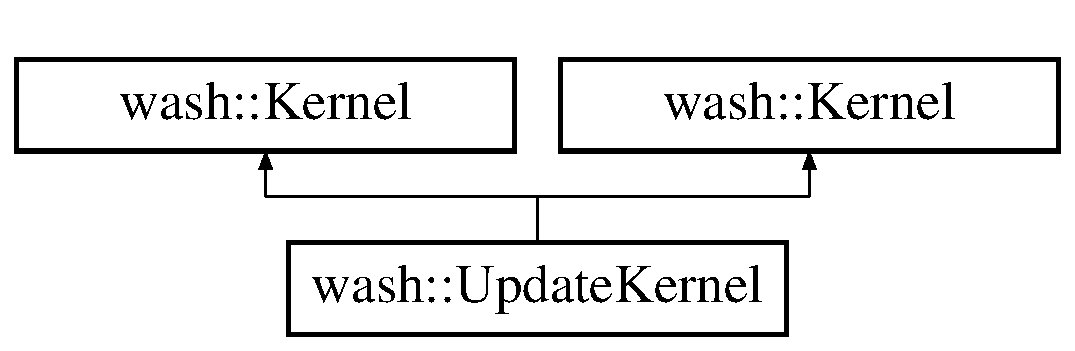
\includegraphics[height=2.000000cm]{classwash_1_1UpdateKernel}
\end{center}
\end{figure}
\subsection*{Public Member Functions}
\begin{DoxyCompactItemize}
\item 
\mbox{\Hypertarget{classwash_1_1UpdateKernel_a2cd95c4f9bcbceff9df7d094f7d7011f}\label{classwash_1_1UpdateKernel_a2cd95c4f9bcbceff9df7d094f7d7011f}} 
{\bfseries Update\+Kernel} (const Update\+FuncT func)
\item 
\mbox{\Hypertarget{classwash_1_1UpdateKernel_a72ec6b0ea453d97708f3fcfd98970366}\label{classwash_1_1UpdateKernel_a72ec6b0ea453d97708f3fcfd98970366}} 
virtual void {\bfseries exec} () const override
\item 
\mbox{\Hypertarget{classwash_1_1UpdateKernel_a2cd95c4f9bcbceff9df7d094f7d7011f}\label{classwash_1_1UpdateKernel_a2cd95c4f9bcbceff9df7d094f7d7011f}} 
{\bfseries Update\+Kernel} (const Update\+FuncT func)
\item 
\mbox{\Hypertarget{classwash_1_1UpdateKernel_a23c7bb181196e107afb1ca4ce9c79137}\label{classwash_1_1UpdateKernel_a23c7bb181196e107afb1ca4ce9c79137}} 
virtual void {\bfseries exec} () const override
\end{DoxyCompactItemize}


The documentation for this class was generated from the following files\+:\begin{DoxyCompactItemize}
\item 
/dcs/20/u2002000/4th\+Year\+Project/wash/src/wash/wash.\+hpp\item 
/dcs/20/u2002000/4th\+Year\+Project/wash/src/wash/wash.\+cpp\end{DoxyCompactItemize}

\hypertarget{classwash_1_1Vec}{}\section{wash\+:\+:Vec$<$ T, dim $>$ Class Template Reference}
\label{classwash_1_1Vec}\index{wash\+::\+Vec$<$ T, dim $>$@{wash\+::\+Vec$<$ T, dim $>$}}
\subsection*{Public Member Functions}
\begin{DoxyCompactItemize}
\item 
\mbox{\Hypertarget{classwash_1_1Vec_a6250ba5f027e9e0e974654136ea7e6ef}\label{classwash_1_1Vec_a6250ba5f027e9e0e974654136ea7e6ef}} 
{\bfseries Vec} (std\+::initializer\+\_\+list$<$ T $>$ l)
\item 
\mbox{\Hypertarget{classwash_1_1Vec_a5927d6caa8489a88b8470fe8bb8779d0}\label{classwash_1_1Vec_a5927d6caa8489a88b8470fe8bb8779d0}} 
T $\ast$ {\bfseries operator\mbox{[}$\,$\mbox{]}} (int i)
\item 
\mbox{\Hypertarget{classwash_1_1Vec_ad8a8863138b26c2b2eae41e11f40e78f}\label{classwash_1_1Vec_ad8a8863138b26c2b2eae41e11f40e78f}} 
\mbox{\hyperlink{classwash_1_1Vec}{Vec}}$<$ T, dim $>$ {\bfseries operator+} (T d)
\item 
\mbox{\Hypertarget{classwash_1_1Vec_a951a842c43b3cf99d60abfe73e53475c}\label{classwash_1_1Vec_a951a842c43b3cf99d60abfe73e53475c}} 
\mbox{\hyperlink{classwash_1_1Vec}{Vec}}$<$ T, dim $>$ {\bfseries operator+} (\mbox{\hyperlink{classwash_1_1Vec}{Vec}}$<$ T, dim $>$ v)
\item 
\mbox{\Hypertarget{classwash_1_1Vec_ac92d90da0a36cdd6b38a8a12e341fa84}\label{classwash_1_1Vec_ac92d90da0a36cdd6b38a8a12e341fa84}} 
void {\bfseries operator+=} (\mbox{\hyperlink{classwash_1_1Vec}{Vec}}$<$ T, dim $>$ v)
\item 
\mbox{\Hypertarget{classwash_1_1Vec_a83a86542f9afb7ea0b5b7b8ab72eb119}\label{classwash_1_1Vec_a83a86542f9afb7ea0b5b7b8ab72eb119}} 
\mbox{\hyperlink{classwash_1_1Vec}{Vec}}$<$ T, dim $>$ {\bfseries operator-\/} (\mbox{\hyperlink{classwash_1_1Vec}{Vec}}$<$ T, dim $>$ v) const
\item 
\mbox{\Hypertarget{classwash_1_1Vec_a972cde51776de1a9efec7ed6ea02f401}\label{classwash_1_1Vec_a972cde51776de1a9efec7ed6ea02f401}} 
\mbox{\hyperlink{classwash_1_1Vec}{Vec}}$<$ T, dim $>$ {\bfseries operator/} (T d)
\item 
\mbox{\Hypertarget{classwash_1_1Vec_a6fc9e30b352c72c7307bd28ee6c0aa72}\label{classwash_1_1Vec_a6fc9e30b352c72c7307bd28ee6c0aa72}} 
\mbox{\hyperlink{classwash_1_1Vec}{Vec}}$<$ T, dim $>$ {\bfseries operator$\ast$} (T d)
\item 
\mbox{\Hypertarget{classwash_1_1Vec_a41de499daf12160b2cf515ce0c9da70f}\label{classwash_1_1Vec_a41de499daf12160b2cf515ce0c9da70f}} 
T {\bfseries magnitude} ()
\item 
\mbox{\Hypertarget{classwash_1_1Vec_a1be26013b6d4f898b8504fc258043400}\label{classwash_1_1Vec_a1be26013b6d4f898b8504fc258043400}} 
T {\bfseries at} (const size\+\_\+t i) const
\item 
\mbox{\Hypertarget{classwash_1_1Vec_aae15a1a2cea7e883e53c2e7f6164710a}\label{classwash_1_1Vec_aae15a1a2cea7e883e53c2e7f6164710a}} 
\mbox{\hyperlink{classwash_1_1Vec}{Vec}}$<$ T, dim $>$ {\bfseries abs} () const
\end{DoxyCompactItemize}


The documentation for this class was generated from the following file\+:\begin{DoxyCompactItemize}
\item 
/dcs/20/u2002000/4th\+Year\+Project/wash/wash\+\_\+vector.\+hpp\end{DoxyCompactItemize}

\hypertarget{classwash_1_1VoidKernel}{}\section{wash\+:\+:Void\+Kernel Class Reference}
\label{classwash_1_1VoidKernel}\index{wash\+::\+Void\+Kernel@{wash\+::\+Void\+Kernel}}


Void \mbox{\hyperlink{classwash_1_1Kernel}{Kernel}} has no arguments/return.  




{\ttfamily \#include $<$kernels.\+hpp$>$}

Inheritance diagram for wash\+:\+:Void\+Kernel\+:\begin{figure}[H]
\begin{center}
\leavevmode
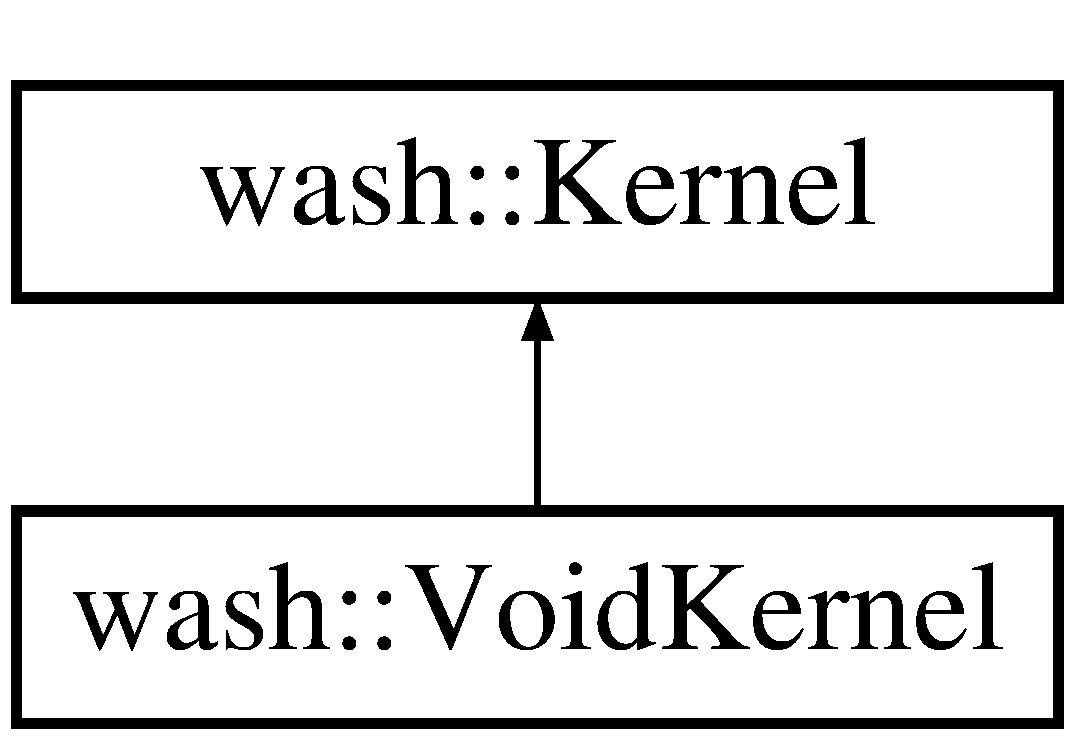
\includegraphics[height=2.000000cm]{classwash_1_1VoidKernel}
\end{center}
\end{figure}
\subsection*{Public Member Functions}
\begin{DoxyCompactItemize}
\item 
\mbox{\Hypertarget{classwash_1_1VoidKernel_abe7159c42c48bf15cf3d69dbf09388dc}\label{classwash_1_1VoidKernel_abe7159c42c48bf15cf3d69dbf09388dc}} 
{\bfseries Void\+Kernel} (const Void\+FuncT func)
\item 
\mbox{\Hypertarget{classwash_1_1VoidKernel_a2a271788509bac47a96dbbecd7fbe90e}\label{classwash_1_1VoidKernel_a2a271788509bac47a96dbbecd7fbe90e}} 
virtual void {\bfseries exec} () const override
\end{DoxyCompactItemize}


\subsection{Detailed Description}
Void \mbox{\hyperlink{classwash_1_1Kernel}{Kernel}} has no arguments/return. 

The documentation for this class was generated from the following files\+:\begin{DoxyCompactItemize}
\item 
/dcs/20/u2002000/4th\+Year\+Project/wash/include/kernels.\+hpp\item 
/dcs/20/u2002000/4th\+Year\+Project/wash/src/impl/cstone/kernels.\+cpp\end{DoxyCompactItemize}

\hypertarget{classws2st_1_1refactor_1_1WashComputationAction}{}\section{ws2st\+:\+:refactor\+:\+:Wash\+Computation\+Action Class Reference}
\label{classws2st_1_1refactor_1_1WashComputationAction}\index{ws2st\+::refactor\+::\+Wash\+Computation\+Action@{ws2st\+::refactor\+::\+Wash\+Computation\+Action}}


Define a function to be run at the end of the refactor pass. Computation Actions will be run in the order they\textquotesingle{}re defined, but will be run after all refactoring actions in the pass have completed.  




{\ttfamily \#include $<$refactor.\+hpp$>$}

\subsection*{Public Member Functions}
\begin{DoxyCompactItemize}
\item 
\mbox{\Hypertarget{classws2st_1_1refactor_1_1WashComputationAction_a5371af5f19e07759f4863e7b6011e787}\label{classws2st_1_1refactor_1_1WashComputationAction_a5371af5f19e07759f4863e7b6011e787}} 
{\bfseries Wash\+Computation\+Action} (Wash\+Compute\+Fn computefn\+\_\+ptr)
\item 
\mbox{\Hypertarget{classws2st_1_1refactor_1_1WashComputationAction_a195edd152f7fd88ca90d6dc7fb4897dc}\label{classws2st_1_1refactor_1_1WashComputationAction_a195edd152f7fd88ca90d6dc7fb4897dc}} 
Wash\+Compute\+Fn {\bfseries get\+Compute\+Fn} ()
\end{DoxyCompactItemize}


\subsection{Detailed Description}
Define a function to be run at the end of the refactor pass. Computation Actions will be run in the order they\textquotesingle{}re defined, but will be run after all refactoring actions in the pass have completed. 

The documentation for this class was generated from the following file\+:\begin{DoxyCompactItemize}
\item 
/dcs/20/u2002000/4th\+Year\+Project/wash/src/ws2st/\mbox{\hyperlink{refactor_8hpp}{refactor.\+hpp}}\end{DoxyCompactItemize}

\hypertarget{classws2st_1_1refactor_1_1WashMatchCallback}{}\section{ws2st\+:\+:refactor\+:\+:Wash\+Match\+Callback Class Reference}
\label{classws2st_1_1refactor_1_1WashMatchCallback}\index{ws2st\+::refactor\+::\+Wash\+Match\+Callback@{ws2st\+::refactor\+::\+Wash\+Match\+Callback}}


A specialised refactoring callback type for Wash using custom function pointers instead of subclassing tooling\+::\+Refactoring\+Callback and implementing ...\+::run a million times.  




{\ttfamily \#include $<$refactor.\+hpp$>$}

Inheritance diagram for ws2st\+:\+:refactor\+:\+:Wash\+Match\+Callback\+:\begin{figure}[H]
\begin{center}
\leavevmode
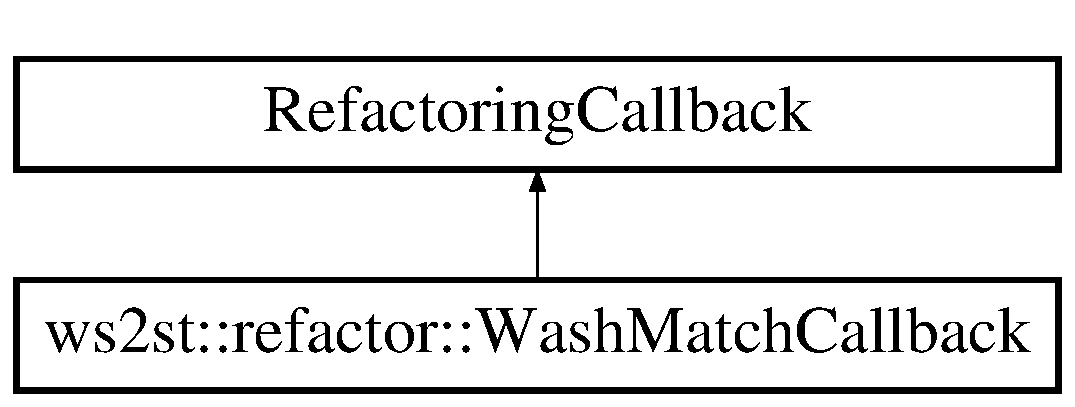
\includegraphics[height=2.000000cm]{classws2st_1_1refactor_1_1WashMatchCallback}
\end{center}
\end{figure}
\subsection*{Public Member Functions}
\begin{DoxyCompactItemize}
\item 
\mbox{\hyperlink{classws2st_1_1refactor_1_1WashMatchCallback_a92cc5cf8562d6d0df12547a5df116bec}{Wash\+Match\+Callback}} (\mbox{\hyperlink{namespacews2st_a682dfda40d8282c7e579a7b826a7d861}{Wash\+Callback\+Fn}} callback\+\_\+ptr)
\item 
virtual void \mbox{\hyperlink{classws2st_1_1refactor_1_1WashMatchCallback_a1712bb28c2728b43b5ca0f2d682382a6}{run}} (const Match\+Finder\+::\+Match\+Result \&Result)
\item 
\mbox{\hyperlink{namespacews2st_a682dfda40d8282c7e579a7b826a7d861}{Wash\+Callback\+Fn}} \mbox{\hyperlink{classws2st_1_1refactor_1_1WashMatchCallback_a91f255d66c7a62daa588b7f6910b5b50}{get\+Callback}} ()
\end{DoxyCompactItemize}
\subsection*{Friends}
\begin{DoxyCompactItemize}
\item 
std\+::ostream \& \mbox{\hyperlink{classws2st_1_1refactor_1_1WashMatchCallback_a0038f6cb22cb01fa32430f4857862513}{operator$<$$<$}} (std\+::ostream \&os, const \mbox{\hyperlink{classws2st_1_1refactor_1_1WashMatchCallback}{Wash\+Match\+Callback}} \&obj)
\end{DoxyCompactItemize}


\subsection{Detailed Description}
A specialised refactoring callback type for Wash using custom function pointers instead of subclassing tooling\+::\+Refactoring\+Callback and implementing ...\+::run a million times. 

\subsection{Constructor \& Destructor Documentation}
\mbox{\Hypertarget{classws2st_1_1refactor_1_1WashMatchCallback_a92cc5cf8562d6d0df12547a5df116bec}\label{classws2st_1_1refactor_1_1WashMatchCallback_a92cc5cf8562d6d0df12547a5df116bec}} 
\index{ws2st\+::refactor\+::\+Wash\+Match\+Callback@{ws2st\+::refactor\+::\+Wash\+Match\+Callback}!Wash\+Match\+Callback@{Wash\+Match\+Callback}}
\index{Wash\+Match\+Callback@{Wash\+Match\+Callback}!ws2st\+::refactor\+::\+Wash\+Match\+Callback@{ws2st\+::refactor\+::\+Wash\+Match\+Callback}}
\subsubsection{\texorpdfstring{Wash\+Match\+Callback()}{WashMatchCallback()}}
{\footnotesize\ttfamily ws2st\+::refactor\+::\+Wash\+Match\+Callback\+::\+Wash\+Match\+Callback (\begin{DoxyParamCaption}\item[{\mbox{\hyperlink{namespacews2st_a682dfda40d8282c7e579a7b826a7d861}{Wash\+Callback\+Fn}}}]{callback\+\_\+ptr }\end{DoxyParamCaption})\hspace{0.3cm}{\ttfamily [inline]}}



\subsection{Member Function Documentation}
\mbox{\Hypertarget{classws2st_1_1refactor_1_1WashMatchCallback_a91f255d66c7a62daa588b7f6910b5b50}\label{classws2st_1_1refactor_1_1WashMatchCallback_a91f255d66c7a62daa588b7f6910b5b50}} 
\index{ws2st\+::refactor\+::\+Wash\+Match\+Callback@{ws2st\+::refactor\+::\+Wash\+Match\+Callback}!get\+Callback@{get\+Callback}}
\index{get\+Callback@{get\+Callback}!ws2st\+::refactor\+::\+Wash\+Match\+Callback@{ws2st\+::refactor\+::\+Wash\+Match\+Callback}}
\subsubsection{\texorpdfstring{get\+Callback()}{getCallback()}}
{\footnotesize\ttfamily \mbox{\hyperlink{namespacews2st_a682dfda40d8282c7e579a7b826a7d861}{Wash\+Callback\+Fn}} ws2st\+::refactor\+::\+Wash\+Match\+Callback\+::get\+Callback (\begin{DoxyParamCaption}{ }\end{DoxyParamCaption})\hspace{0.3cm}{\ttfamily [inline]}}

\mbox{\Hypertarget{classws2st_1_1refactor_1_1WashMatchCallback_a1712bb28c2728b43b5ca0f2d682382a6}\label{classws2st_1_1refactor_1_1WashMatchCallback_a1712bb28c2728b43b5ca0f2d682382a6}} 
\index{ws2st\+::refactor\+::\+Wash\+Match\+Callback@{ws2st\+::refactor\+::\+Wash\+Match\+Callback}!run@{run}}
\index{run@{run}!ws2st\+::refactor\+::\+Wash\+Match\+Callback@{ws2st\+::refactor\+::\+Wash\+Match\+Callback}}
\subsubsection{\texorpdfstring{run()}{run()}}
{\footnotesize\ttfamily virtual void ws2st\+::refactor\+::\+Wash\+Match\+Callback\+::run (\begin{DoxyParamCaption}\item[{const Match\+Finder\+::\+Match\+Result \&}]{Result }\end{DoxyParamCaption})\hspace{0.3cm}{\ttfamily [inline]}, {\ttfamily [virtual]}}



\subsection{Friends And Related Function Documentation}
\mbox{\Hypertarget{classws2st_1_1refactor_1_1WashMatchCallback_a0038f6cb22cb01fa32430f4857862513}\label{classws2st_1_1refactor_1_1WashMatchCallback_a0038f6cb22cb01fa32430f4857862513}} 
\index{ws2st\+::refactor\+::\+Wash\+Match\+Callback@{ws2st\+::refactor\+::\+Wash\+Match\+Callback}!operator$<$$<$@{operator$<$$<$}}
\index{operator$<$$<$@{operator$<$$<$}!ws2st\+::refactor\+::\+Wash\+Match\+Callback@{ws2st\+::refactor\+::\+Wash\+Match\+Callback}}
\subsubsection{\texorpdfstring{operator$<$$<$}{operator<<}}
{\footnotesize\ttfamily std\+::ostream\& operator$<$$<$ (\begin{DoxyParamCaption}\item[{std\+::ostream \&}]{os,  }\item[{const \mbox{\hyperlink{classws2st_1_1refactor_1_1WashMatchCallback}{Wash\+Match\+Callback}} \&}]{obj }\end{DoxyParamCaption})\hspace{0.3cm}{\ttfamily [friend]}}



The documentation for this class was generated from the following file\+:\begin{DoxyCompactItemize}
\item 
/dcs/20/u2002000/4th\+Year\+Project/wash/src/ws2st/\mbox{\hyperlink{refactor_8hpp}{refactor.\+hpp}}\end{DoxyCompactItemize}

\hypertarget{structWashOptions}{}\section{Wash\+Options Struct Reference}
\label{structWashOptions}\index{Wash\+Options@{Wash\+Options}}


Options about how the Wash analysis will behave.  




{\ttfamily \#include $<$common.\+hpp$>$}

\subsection*{Public Attributes}
\begin{DoxyCompactItemize}
\item 
\mbox{\hyperlink{common_8hpp_aad9d1428f17c06ff77ef15dea22624dc}{Implementations}} \mbox{\hyperlink{structWashOptions_a44a1b923dc5034a3bf45dee2f54623ca}{impl}}
\item 
bool \mbox{\hyperlink{structWashOptions_a50d97883a6c0eaf8bafda97f5bad2a1e}{openmp}}
\item 
bool \mbox{\hyperlink{structWashOptions_a9ec267278d89d04982e3d70e877d5c67}{mpi}}
\item 
bool \mbox{\hyperlink{structWashOptions_a31ed802896363b97ac1f5199a6940df9}{hdf5}}
\item 
bool \mbox{\hyperlink{structWashOptions_a5bc365ad8fc0544864d15709b6808843}{debug}}
\item 
uint8\+\_\+t \mbox{\hyperlink{structWashOptions_a0caa33c545fc380c4104ca90f6462dfb}{dim}}
\item 
std\+::string \mbox{\hyperlink{structWashOptions_a4b43b8f0700908a6975a367d2cb9d567}{input\+\_\+path}}
\item 
std\+::string \mbox{\hyperlink{structWashOptions_a091c31f0eee54c7b079268f7a1001547}{output\+\_\+name}}
\item 
std\+::string \mbox{\hyperlink{structWashOptions_a27f59d7e66cdf80f0fe5cc5e699b0953}{temp\+\_\+path}}
\item 
std\+::vector$<$ std\+::string $>$ \mbox{\hyperlink{structWashOptions_abc32ad74441fbc82069b4addc130d4cd}{args}}
\end{DoxyCompactItemize}


\subsection{Detailed Description}
Options about how the Wash analysis will behave. 

Whether to enable certain features via flags in the compiler analysis and then again in the final compilation stages.

T\+O\+DO\+: If multiple options are enabled which are contradictory, then we should generate multiple output binaries at the end. 

\subsection{Member Data Documentation}
\mbox{\Hypertarget{structWashOptions_abc32ad74441fbc82069b4addc130d4cd}\label{structWashOptions_abc32ad74441fbc82069b4addc130d4cd}} 
\index{Wash\+Options@{Wash\+Options}!args@{args}}
\index{args@{args}!Wash\+Options@{Wash\+Options}}
\subsubsection{\texorpdfstring{args}{args}}
{\footnotesize\ttfamily std\+::vector$<$std\+::string$>$ Wash\+Options\+::args}

\mbox{\Hypertarget{structWashOptions_a5bc365ad8fc0544864d15709b6808843}\label{structWashOptions_a5bc365ad8fc0544864d15709b6808843}} 
\index{Wash\+Options@{Wash\+Options}!debug@{debug}}
\index{debug@{debug}!Wash\+Options@{Wash\+Options}}
\subsubsection{\texorpdfstring{debug}{debug}}
{\footnotesize\ttfamily bool Wash\+Options\+::debug}

\mbox{\Hypertarget{structWashOptions_a0caa33c545fc380c4104ca90f6462dfb}\label{structWashOptions_a0caa33c545fc380c4104ca90f6462dfb}} 
\index{Wash\+Options@{Wash\+Options}!dim@{dim}}
\index{dim@{dim}!Wash\+Options@{Wash\+Options}}
\subsubsection{\texorpdfstring{dim}{dim}}
{\footnotesize\ttfamily uint8\+\_\+t Wash\+Options\+::dim}

\mbox{\Hypertarget{structWashOptions_a31ed802896363b97ac1f5199a6940df9}\label{structWashOptions_a31ed802896363b97ac1f5199a6940df9}} 
\index{Wash\+Options@{Wash\+Options}!hdf5@{hdf5}}
\index{hdf5@{hdf5}!Wash\+Options@{Wash\+Options}}
\subsubsection{\texorpdfstring{hdf5}{hdf5}}
{\footnotesize\ttfamily bool Wash\+Options\+::hdf5}

\mbox{\Hypertarget{structWashOptions_a44a1b923dc5034a3bf45dee2f54623ca}\label{structWashOptions_a44a1b923dc5034a3bf45dee2f54623ca}} 
\index{Wash\+Options@{Wash\+Options}!impl@{impl}}
\index{impl@{impl}!Wash\+Options@{Wash\+Options}}
\subsubsection{\texorpdfstring{impl}{impl}}
{\footnotesize\ttfamily \mbox{\hyperlink{common_8hpp_aad9d1428f17c06ff77ef15dea22624dc}{Implementations}} Wash\+Options\+::impl}

\mbox{\Hypertarget{structWashOptions_a4b43b8f0700908a6975a367d2cb9d567}\label{structWashOptions_a4b43b8f0700908a6975a367d2cb9d567}} 
\index{Wash\+Options@{Wash\+Options}!input\+\_\+path@{input\+\_\+path}}
\index{input\+\_\+path@{input\+\_\+path}!Wash\+Options@{Wash\+Options}}
\subsubsection{\texorpdfstring{input\+\_\+path}{input\_path}}
{\footnotesize\ttfamily std\+::string Wash\+Options\+::input\+\_\+path}

\mbox{\Hypertarget{structWashOptions_a9ec267278d89d04982e3d70e877d5c67}\label{structWashOptions_a9ec267278d89d04982e3d70e877d5c67}} 
\index{Wash\+Options@{Wash\+Options}!mpi@{mpi}}
\index{mpi@{mpi}!Wash\+Options@{Wash\+Options}}
\subsubsection{\texorpdfstring{mpi}{mpi}}
{\footnotesize\ttfamily bool Wash\+Options\+::mpi}

\mbox{\Hypertarget{structWashOptions_a50d97883a6c0eaf8bafda97f5bad2a1e}\label{structWashOptions_a50d97883a6c0eaf8bafda97f5bad2a1e}} 
\index{Wash\+Options@{Wash\+Options}!openmp@{openmp}}
\index{openmp@{openmp}!Wash\+Options@{Wash\+Options}}
\subsubsection{\texorpdfstring{openmp}{openmp}}
{\footnotesize\ttfamily bool Wash\+Options\+::openmp}

\mbox{\Hypertarget{structWashOptions_a091c31f0eee54c7b079268f7a1001547}\label{structWashOptions_a091c31f0eee54c7b079268f7a1001547}} 
\index{Wash\+Options@{Wash\+Options}!output\+\_\+name@{output\+\_\+name}}
\index{output\+\_\+name@{output\+\_\+name}!Wash\+Options@{Wash\+Options}}
\subsubsection{\texorpdfstring{output\+\_\+name}{output\_name}}
{\footnotesize\ttfamily std\+::string Wash\+Options\+::output\+\_\+name}

\mbox{\Hypertarget{structWashOptions_a27f59d7e66cdf80f0fe5cc5e699b0953}\label{structWashOptions_a27f59d7e66cdf80f0fe5cc5e699b0953}} 
\index{Wash\+Options@{Wash\+Options}!temp\+\_\+path@{temp\+\_\+path}}
\index{temp\+\_\+path@{temp\+\_\+path}!Wash\+Options@{Wash\+Options}}
\subsubsection{\texorpdfstring{temp\+\_\+path}{temp\_path}}
{\footnotesize\ttfamily std\+::string Wash\+Options\+::temp\+\_\+path}



The documentation for this struct was generated from the following file\+:\begin{DoxyCompactItemize}
\item 
/dcs/20/u2002000/4th\+Year\+Project/wash/src/ws2st/\mbox{\hyperlink{common_8hpp}{common.\+hpp}}\end{DoxyCompactItemize}

\hypertarget{structws2st_1_1WashProgramMeta}{}\section{ws2st\+:\+:Wash\+Program\+Meta Struct Reference}
\label{structws2st_1_1WashProgramMeta}\index{ws2st\+::\+Wash\+Program\+Meta@{ws2st\+::\+Wash\+Program\+Meta}}


Meta information about the simulation which is defined globally and can be read/written to by the callback functions.  




{\ttfamily \#include $<$common.\+hpp$>$}

\subsection*{Public Attributes}
\begin{DoxyCompactItemize}
\item 
std\+::vector$<$ std\+::string $>$ \mbox{\hyperlink{structws2st_1_1WashProgramMeta_a71dfe0ec3a593707b26a3387d6ffe097}{scalar\+\_\+force\+\_\+list}}
\item 
std\+::vector$<$ std\+::string $>$ \mbox{\hyperlink{structws2st_1_1WashProgramMeta_a4b2ccb325270ac70589972a556b704b5}{vector\+\_\+force\+\_\+list}}
\item 
std\+::unordered\+\_\+map$<$ std\+::string, Full\+Source\+Loc $>$ \mbox{\hyperlink{structws2st_1_1WashProgramMeta_a2769172e26989f7d8759906460bbd43c}{force\+\_\+meta}}
\item 
std\+::vector$<$ std\+::pair$<$ std\+::string, std\+::string $>$ $>$ \mbox{\hyperlink{structws2st_1_1WashProgramMeta_ac42b81ba6becd8cba9834dc903704e5c}{variable\+\_\+list}}
\item 
int \mbox{\hyperlink{structws2st_1_1WashProgramMeta_a3a521dc326a6070a0af9c4bbec3913f4}{simulation\+\_\+dimension}}
\item 
std\+::vector$<$ std\+::string $>$ \mbox{\hyperlink{structws2st_1_1WashProgramMeta_ae19b95e2db30a6d8b366b1c9965b4806}{kernels\+\_\+list}}
\item 
std\+::vector$<$ std\+::string $>$ \mbox{\hyperlink{structws2st_1_1WashProgramMeta_a36d24273393b878a32f470aff4cd837f}{init\+\_\+kernels\+\_\+list}}
\item 
std\+::string \mbox{\hyperlink{structws2st_1_1WashProgramMeta_ab8b551d40c83ad55f84610e7041972cd}{neighbour\+\_\+kernel}}
\item 
std\+::unordered\+\_\+map$<$ std\+::string, std\+::unique\+\_\+ptr$<$ \mbox{\hyperlink{structws2st_1_1KernelDependencies}{Kernel\+Dependencies}} $>$ $>$ \mbox{\hyperlink{structws2st_1_1WashProgramMeta_a3f60907c890b351559afda6420edf367}{kernels\+\_\+dependency\+\_\+map}}
\item 
std\+::vector$<$ bool $>$ \mbox{\hyperlink{structws2st_1_1WashProgramMeta_aa6a9a7afafcc71c0e39e87b6af2216a1}{domain\+\_\+sync\+\_\+locations}}
\item 
std\+::vector$<$ bool $>$ \mbox{\hyperlink{structws2st_1_1WashProgramMeta_a43cc6c30c364f4b03c79189998368ad4}{domain\+\_\+sync\+\_\+before}}
\end{DoxyCompactItemize}


\subsection{Detailed Description}
Meta information about the simulation which is defined globally and can be read/written to by the callback functions. 

\subsection{Member Data Documentation}
\mbox{\Hypertarget{structws2st_1_1WashProgramMeta_a43cc6c30c364f4b03c79189998368ad4}\label{structws2st_1_1WashProgramMeta_a43cc6c30c364f4b03c79189998368ad4}} 
\index{ws2st\+::\+Wash\+Program\+Meta@{ws2st\+::\+Wash\+Program\+Meta}!domain\+\_\+sync\+\_\+before@{domain\+\_\+sync\+\_\+before}}
\index{domain\+\_\+sync\+\_\+before@{domain\+\_\+sync\+\_\+before}!ws2st\+::\+Wash\+Program\+Meta@{ws2st\+::\+Wash\+Program\+Meta}}
\subsubsection{\texorpdfstring{domain\+\_\+sync\+\_\+before}{domain\_sync\_before}}
{\footnotesize\ttfamily std\+::vector$<$bool$>$ ws2st\+::\+Wash\+Program\+Meta\+::domain\+\_\+sync\+\_\+before}

\mbox{\Hypertarget{structws2st_1_1WashProgramMeta_aa6a9a7afafcc71c0e39e87b6af2216a1}\label{structws2st_1_1WashProgramMeta_aa6a9a7afafcc71c0e39e87b6af2216a1}} 
\index{ws2st\+::\+Wash\+Program\+Meta@{ws2st\+::\+Wash\+Program\+Meta}!domain\+\_\+sync\+\_\+locations@{domain\+\_\+sync\+\_\+locations}}
\index{domain\+\_\+sync\+\_\+locations@{domain\+\_\+sync\+\_\+locations}!ws2st\+::\+Wash\+Program\+Meta@{ws2st\+::\+Wash\+Program\+Meta}}
\subsubsection{\texorpdfstring{domain\+\_\+sync\+\_\+locations}{domain\_sync\_locations}}
{\footnotesize\ttfamily std\+::vector$<$bool$>$ ws2st\+::\+Wash\+Program\+Meta\+::domain\+\_\+sync\+\_\+locations}

\mbox{\Hypertarget{structws2st_1_1WashProgramMeta_a2769172e26989f7d8759906460bbd43c}\label{structws2st_1_1WashProgramMeta_a2769172e26989f7d8759906460bbd43c}} 
\index{ws2st\+::\+Wash\+Program\+Meta@{ws2st\+::\+Wash\+Program\+Meta}!force\+\_\+meta@{force\+\_\+meta}}
\index{force\+\_\+meta@{force\+\_\+meta}!ws2st\+::\+Wash\+Program\+Meta@{ws2st\+::\+Wash\+Program\+Meta}}
\subsubsection{\texorpdfstring{force\+\_\+meta}{force\_meta}}
{\footnotesize\ttfamily std\+::unordered\+\_\+map$<$std\+::string, Full\+Source\+Loc$>$ ws2st\+::\+Wash\+Program\+Meta\+::force\+\_\+meta}

\mbox{\Hypertarget{structws2st_1_1WashProgramMeta_a36d24273393b878a32f470aff4cd837f}\label{structws2st_1_1WashProgramMeta_a36d24273393b878a32f470aff4cd837f}} 
\index{ws2st\+::\+Wash\+Program\+Meta@{ws2st\+::\+Wash\+Program\+Meta}!init\+\_\+kernels\+\_\+list@{init\+\_\+kernels\+\_\+list}}
\index{init\+\_\+kernels\+\_\+list@{init\+\_\+kernels\+\_\+list}!ws2st\+::\+Wash\+Program\+Meta@{ws2st\+::\+Wash\+Program\+Meta}}
\subsubsection{\texorpdfstring{init\+\_\+kernels\+\_\+list}{init\_kernels\_list}}
{\footnotesize\ttfamily std\+::vector$<$std\+::string$>$ ws2st\+::\+Wash\+Program\+Meta\+::init\+\_\+kernels\+\_\+list}

\mbox{\Hypertarget{structws2st_1_1WashProgramMeta_a3f60907c890b351559afda6420edf367}\label{structws2st_1_1WashProgramMeta_a3f60907c890b351559afda6420edf367}} 
\index{ws2st\+::\+Wash\+Program\+Meta@{ws2st\+::\+Wash\+Program\+Meta}!kernels\+\_\+dependency\+\_\+map@{kernels\+\_\+dependency\+\_\+map}}
\index{kernels\+\_\+dependency\+\_\+map@{kernels\+\_\+dependency\+\_\+map}!ws2st\+::\+Wash\+Program\+Meta@{ws2st\+::\+Wash\+Program\+Meta}}
\subsubsection{\texorpdfstring{kernels\+\_\+dependency\+\_\+map}{kernels\_dependency\_map}}
{\footnotesize\ttfamily std\+::unordered\+\_\+map$<$std\+::string, std\+::unique\+\_\+ptr$<$\mbox{\hyperlink{structws2st_1_1KernelDependencies}{Kernel\+Dependencies}}$>$ $>$ ws2st\+::\+Wash\+Program\+Meta\+::kernels\+\_\+dependency\+\_\+map}

\mbox{\Hypertarget{structws2st_1_1WashProgramMeta_ae19b95e2db30a6d8b366b1c9965b4806}\label{structws2st_1_1WashProgramMeta_ae19b95e2db30a6d8b366b1c9965b4806}} 
\index{ws2st\+::\+Wash\+Program\+Meta@{ws2st\+::\+Wash\+Program\+Meta}!kernels\+\_\+list@{kernels\+\_\+list}}
\index{kernels\+\_\+list@{kernels\+\_\+list}!ws2st\+::\+Wash\+Program\+Meta@{ws2st\+::\+Wash\+Program\+Meta}}
\subsubsection{\texorpdfstring{kernels\+\_\+list}{kernels\_list}}
{\footnotesize\ttfamily std\+::vector$<$std\+::string$>$ ws2st\+::\+Wash\+Program\+Meta\+::kernels\+\_\+list}

\mbox{\Hypertarget{structws2st_1_1WashProgramMeta_ab8b551d40c83ad55f84610e7041972cd}\label{structws2st_1_1WashProgramMeta_ab8b551d40c83ad55f84610e7041972cd}} 
\index{ws2st\+::\+Wash\+Program\+Meta@{ws2st\+::\+Wash\+Program\+Meta}!neighbour\+\_\+kernel@{neighbour\+\_\+kernel}}
\index{neighbour\+\_\+kernel@{neighbour\+\_\+kernel}!ws2st\+::\+Wash\+Program\+Meta@{ws2st\+::\+Wash\+Program\+Meta}}
\subsubsection{\texorpdfstring{neighbour\+\_\+kernel}{neighbour\_kernel}}
{\footnotesize\ttfamily std\+::string ws2st\+::\+Wash\+Program\+Meta\+::neighbour\+\_\+kernel}

\mbox{\Hypertarget{structws2st_1_1WashProgramMeta_a71dfe0ec3a593707b26a3387d6ffe097}\label{structws2st_1_1WashProgramMeta_a71dfe0ec3a593707b26a3387d6ffe097}} 
\index{ws2st\+::\+Wash\+Program\+Meta@{ws2st\+::\+Wash\+Program\+Meta}!scalar\+\_\+force\+\_\+list@{scalar\+\_\+force\+\_\+list}}
\index{scalar\+\_\+force\+\_\+list@{scalar\+\_\+force\+\_\+list}!ws2st\+::\+Wash\+Program\+Meta@{ws2st\+::\+Wash\+Program\+Meta}}
\subsubsection{\texorpdfstring{scalar\+\_\+force\+\_\+list}{scalar\_force\_list}}
{\footnotesize\ttfamily std\+::vector$<$std\+::string$>$ ws2st\+::\+Wash\+Program\+Meta\+::scalar\+\_\+force\+\_\+list}

\mbox{\Hypertarget{structws2st_1_1WashProgramMeta_a3a521dc326a6070a0af9c4bbec3913f4}\label{structws2st_1_1WashProgramMeta_a3a521dc326a6070a0af9c4bbec3913f4}} 
\index{ws2st\+::\+Wash\+Program\+Meta@{ws2st\+::\+Wash\+Program\+Meta}!simulation\+\_\+dimension@{simulation\+\_\+dimension}}
\index{simulation\+\_\+dimension@{simulation\+\_\+dimension}!ws2st\+::\+Wash\+Program\+Meta@{ws2st\+::\+Wash\+Program\+Meta}}
\subsubsection{\texorpdfstring{simulation\+\_\+dimension}{simulation\_dimension}}
{\footnotesize\ttfamily int ws2st\+::\+Wash\+Program\+Meta\+::simulation\+\_\+dimension}

\mbox{\Hypertarget{structws2st_1_1WashProgramMeta_ac42b81ba6becd8cba9834dc903704e5c}\label{structws2st_1_1WashProgramMeta_ac42b81ba6becd8cba9834dc903704e5c}} 
\index{ws2st\+::\+Wash\+Program\+Meta@{ws2st\+::\+Wash\+Program\+Meta}!variable\+\_\+list@{variable\+\_\+list}}
\index{variable\+\_\+list@{variable\+\_\+list}!ws2st\+::\+Wash\+Program\+Meta@{ws2st\+::\+Wash\+Program\+Meta}}
\subsubsection{\texorpdfstring{variable\+\_\+list}{variable\_list}}
{\footnotesize\ttfamily std\+::vector$<$std\+::pair$<$std\+::string, std\+::string$>$ $>$ ws2st\+::\+Wash\+Program\+Meta\+::variable\+\_\+list}

\mbox{\Hypertarget{structws2st_1_1WashProgramMeta_a4b2ccb325270ac70589972a556b704b5}\label{structws2st_1_1WashProgramMeta_a4b2ccb325270ac70589972a556b704b5}} 
\index{ws2st\+::\+Wash\+Program\+Meta@{ws2st\+::\+Wash\+Program\+Meta}!vector\+\_\+force\+\_\+list@{vector\+\_\+force\+\_\+list}}
\index{vector\+\_\+force\+\_\+list@{vector\+\_\+force\+\_\+list}!ws2st\+::\+Wash\+Program\+Meta@{ws2st\+::\+Wash\+Program\+Meta}}
\subsubsection{\texorpdfstring{vector\+\_\+force\+\_\+list}{vector\_force\_list}}
{\footnotesize\ttfamily std\+::vector$<$std\+::string$>$ ws2st\+::\+Wash\+Program\+Meta\+::vector\+\_\+force\+\_\+list}



The documentation for this struct was generated from the following file\+:\begin{DoxyCompactItemize}
\item 
/dcs/20/u2002000/4th\+Year\+Project/wash/src/ws2st/\mbox{\hyperlink{common_8hpp}{common.\+hpp}}\end{DoxyCompactItemize}

\hypertarget{classws2st_1_1refactor_1_1WashRefactoringAction}{}\section{ws2st\+:\+:refactor\+:\+:Wash\+Refactoring\+Action Class Reference}
\label{classws2st_1_1refactor_1_1WashRefactoringAction}\index{ws2st\+::refactor\+::\+Wash\+Refactoring\+Action@{ws2st\+::refactor\+::\+Wash\+Refactoring\+Action}}


Developer defined registration of a refactoring action -\/ a ($<$\+T$>$Matcher, Callback\+Fn) pair.  




{\ttfamily \#include $<$refactor.\+hpp$>$}

\subsection*{Public Member Functions}
\begin{DoxyCompactItemize}
\item 
\mbox{\Hypertarget{classws2st_1_1refactor_1_1WashRefactoringAction_a37b89a13a8e91735717cc1df37e8eabb}\label{classws2st_1_1refactor_1_1WashRefactoringAction_a37b89a13a8e91735717cc1df37e8eabb}} 
{\bfseries Wash\+Refactoring\+Action} (Statement\+Matcher $\ast$matcher\+\_\+ptr, Wash\+Callback\+Fn callback\+\_\+ptr)
\item 
\mbox{\Hypertarget{classws2st_1_1refactor_1_1WashRefactoringAction_a5ebcf97bf4b5fec82c4a9c931b61ae2b}\label{classws2st_1_1refactor_1_1WashRefactoringAction_a5ebcf97bf4b5fec82c4a9c931b61ae2b}} 
{\bfseries Wash\+Refactoring\+Action} (Declaration\+Matcher $\ast$matcher\+\_\+ptr, Wash\+Callback\+Fn callback\+\_\+ptr)
\item 
\mbox{\Hypertarget{classws2st_1_1refactor_1_1WashRefactoringAction_aaf97a9edbe147cb2d5697d28c5485924}\label{classws2st_1_1refactor_1_1WashRefactoringAction_aaf97a9edbe147cb2d5697d28c5485924}} 
Wash\+Callback\+Fn {\bfseries get\+Callback\+Fn} ()
\item 
\mbox{\Hypertarget{classws2st_1_1refactor_1_1WashRefactoringAction_a22a440b7927da3ab1561a9292b9ee0d6}\label{classws2st_1_1refactor_1_1WashRefactoringAction_a22a440b7927da3ab1561a9292b9ee0d6}} 
std\+::variant$<$ Statement\+Matcher $\ast$, Declaration\+Matcher $\ast$ $>$ {\bfseries get\+Matcher} ()
\end{DoxyCompactItemize}


\subsection{Detailed Description}
Developer defined registration of a refactoring action -\/ a ($<$\+T$>$Matcher, Callback\+Fn) pair. 

The documentation for this class was generated from the following file\+:\begin{DoxyCompactItemize}
\item 
/dcs/20/u2002000/4th\+Year\+Project/wash/src/ws2st/\mbox{\hyperlink{refactor_8hpp}{refactor.\+hpp}}\end{DoxyCompactItemize}

\chapter{File Documentation}
\hypertarget{example__usecase_8md}{}\section{markdown/example\+\_\+usecase.md File Reference}
\label{example__usecase_8md}\index{markdown/example\+\_\+usecase.\+md@{markdown/example\+\_\+usecase.\+md}}

\hypertarget{installation_8md}{}\section{markdown/installation.md File Reference}
\label{installation_8md}\index{markdown/installation.\+md@{markdown/installation.\+md}}

\hypertarget{main__page_8md}{}\section{markdown/main\+\_\+page.md File Reference}
\label{main__page_8md}\index{markdown/main\+\_\+page.\+md@{markdown/main\+\_\+page.\+md}}

\hypertarget{markdown__test_8md}{}\section{markdown/markdown\+\_\+test.md File Reference}
\label{markdown__test_8md}\index{markdown/markdown\+\_\+test.\+md@{markdown/markdown\+\_\+test.\+md}}

\hypertarget{create__gif_8py}{}\section{/dcs/20/u2002000/4th\+Year\+Project/wash/create\+\_\+gif.py File Reference}
\label{create__gif_8py}\index{/dcs/20/u2002000/4th\+Year\+Project/wash/create\+\_\+gif.\+py@{/dcs/20/u2002000/4th\+Year\+Project/wash/create\+\_\+gif.\+py}}
\subsection*{Namespaces}
\begin{DoxyCompactItemize}
\item 
 \mbox{\hyperlink{namespacecreate__gif}{create\+\_\+gif}}
\end{DoxyCompactItemize}
\subsection*{Functions}
\begin{DoxyCompactItemize}
\item 
def \mbox{\hyperlink{namespacecreate__gif_ab64559b25583d234fb61bd16db7e14cc}{create\+\_\+gif.\+create\+\_\+gif\+\_\+from\+\_\+png}} (path\+\_\+name, frame\+\_\+count, output)
\end{DoxyCompactItemize}
\subsection*{Variables}
\begin{DoxyCompactItemize}
\item 
\mbox{\hyperlink{namespacecreate__gif_aab19cf44cc2d4d83200c29825b881639}{create\+\_\+gif.\+path\+\_\+name}} = input(\char`\"{}Input Path (no ext)\+: \char`\"{})
\item 
\mbox{\hyperlink{namespacecreate__gif_abac19e3a427fb292d807a5f270d9b1bf}{create\+\_\+gif.\+frame\+\_\+count}} = int(input(\char`\"{}Frame count\+: \char`\"{}))
\item 
\mbox{\hyperlink{namespacecreate__gif_ab6dfc2d61e95d5ee061db577c2474ad9}{create\+\_\+gif.\+output}} = input(\char`\"{}Output Path (no ext)\+: \char`\"{})
\end{DoxyCompactItemize}

\hypertarget{ascii_8hpp}{}\section{/dcs/20/u2002000/4th\+Year\+Project/wash/include/ascii.hpp File Reference}
\label{ascii_8hpp}\index{/dcs/20/u2002000/4th\+Year\+Project/wash/include/ascii.\+hpp@{/dcs/20/u2002000/4th\+Year\+Project/wash/include/ascii.\+hpp}}
{\ttfamily \#include \char`\"{}io.\+hpp\char`\"{}}\newline
\subsection*{Namespaces}
\begin{DoxyCompactItemize}
\item 
 \mbox{\hyperlink{namespacewash}{wash}}
\begin{DoxyCompactList}\small\item\em T\+O\+DO\+: Consider having this as a private header in W\+I\+S\+B/\+W\+S2\+S\+T/etc implementations. \end{DoxyCompactList}\item 
 \mbox{\hyperlink{namespacewash_1_1io}{wash\+::io}}
\end{DoxyCompactItemize}
\subsection*{Functions}
\begin{DoxyCompactItemize}
\item 
int \mbox{\hyperlink{namespacewash_1_1io_ab29d891bfd64999f5ffb3aa5b13c5b22}{wash\+::io\+::write\+\_\+ascii}} (const I\+O\+Manager \&io, const Simulation\+Data \&sim\+\_\+data, size\+\_\+t iter)
\begin{DoxyCompactList}\small\item\em Write A\+S\+C\+II Output. \end{DoxyCompactList}\end{DoxyCompactItemize}

\hypertarget{hdf5_8hpp}{}\section{/dcs/20/u2002000/4th\+Year\+Project/wash/include/hdf5.hpp File Reference}
\label{hdf5_8hpp}\index{/dcs/20/u2002000/4th\+Year\+Project/wash/include/hdf5.\+hpp@{/dcs/20/u2002000/4th\+Year\+Project/wash/include/hdf5.\+hpp}}
{\ttfamily \#include \char`\"{}io.\+hpp\char`\"{}}\newline

\hypertarget{io_8hpp}{}\section{/dcs/20/u2002000/4th\+Year\+Project/wash/include/io.hpp File Reference}
\label{io_8hpp}\index{/dcs/20/u2002000/4th\+Year\+Project/wash/include/io.\+hpp@{/dcs/20/u2002000/4th\+Year\+Project/wash/include/io.\+hpp}}
{\ttfamily \#include $<$iostream$>$}\newline
{\ttfamily \#include $<$filesystem$>$}\newline
{\ttfamily \#include $<$fstream$>$}\newline
{\ttfamily \#include $<$stdint.\+h$>$}\newline
{\ttfamily \#include $<$limits.\+h$>$}\newline
{\ttfamily \#include $<$unordered\+\_\+map$>$}\newline
{\ttfamily \#include \char`\"{}wash.\+hpp\char`\"{}}\newline
{\ttfamily \#include \char`\"{}vector.\+hpp\char`\"{}}\newline
{\ttfamily \#include \char`\"{}particle\+\_\+data.\+hpp\char`\"{}}\newline
\subsection*{Classes}
\begin{DoxyCompactItemize}
\item 
struct \mbox{\hyperlink{structwash_1_1io_1_1SimulationData}{wash\+::io\+::\+Simulation\+Data}}
\item 
class \mbox{\hyperlink{classwash_1_1io_1_1IOManager}{wash\+::io\+::\+I\+O\+Manager}}
\begin{DoxyCompactList}\small\item\em Manages the IO options for the simulation. \end{DoxyCompactList}\end{DoxyCompactItemize}
\subsection*{Namespaces}
\begin{DoxyCompactItemize}
\item 
 \mbox{\hyperlink{namespacewash}{wash}}
\begin{DoxyCompactList}\small\item\em T\+O\+DO\+: Consider having this as a private header in W\+I\+S\+B/\+W\+S2\+S\+T/etc implementations. \end{DoxyCompactList}\item 
 \mbox{\hyperlink{namespacewash_1_1io}{wash\+::io}}
\end{DoxyCompactItemize}
\subsection*{Macros}
\begin{DoxyCompactItemize}
\item 
\#define \mbox{\hyperlink{io_8hpp_aaae430420e25984e327a89b068e1582b}{M\+P\+I\+\_\+\+S\+I\+Z\+E\+\_\+T}}~M\+P\+I\+\_\+\+U\+N\+S\+I\+G\+N\+E\+D\+\_\+\+C\+H\+AR
\end{DoxyCompactItemize}
\subsection*{Functions}
\begin{DoxyCompactItemize}
\item 
const std\+::string \mbox{\hyperlink{namespacewash_1_1io_a8976ca6dfe3e6332440f2627928db7f9}{wash\+::io\+::get\+\_\+simulation\+\_\+name}} ()
\item 
const std\+::string \mbox{\hyperlink{namespacewash_1_1io_af034a23a15be4666c01bc18c86a45e3e}{wash\+::io\+::get\+\_\+output\+\_\+name}} ()
\item 
Simulation\+Data \mbox{\hyperlink{namespacewash_1_1io_aa9be91ca55f718793aa2e38512d6bdab}{wash\+::io\+::copy\+\_\+simulation\+\_\+data}} ()
\item 
I\+O\+Manager\+::\+Writer\+FuncT \mbox{\hyperlink{namespacewash_1_1io_ac3ef6862cb415612f2bd0f102459511e}{wash\+::io\+::return\+\_\+writer}} (const std\+::string format)
\item 
io\+::\+I\+O\+Manager \mbox{\hyperlink{namespacewash_a92e4e768dbd609eba32fc0d68977d42f}{wash\+::create\+\_\+io}} (const std\+::string format, const size\+\_\+t output\+\_\+nth, const bool use\+\_\+gather=false, const size\+\_\+t rank=0, const size\+\_\+t \mbox{\hyperlink{consts_8cpp_ae8542fe44413919dee9f41ede5a5032d}{size}}=1, const bool timings=true)
\begin{DoxyCompactList}\small\item\em Set-\/up the IO options for the simulation. \end{DoxyCompactList}\item 
std\+::vector$<$ double $>$ \mbox{\hyperlink{namespacewash_afb1cc65bb4ecf6112723b4fb95450c96}{wash\+::copy\+\_\+variables}} ()
\begin{DoxyCompactList}\small\item\em Copy the variables of the simulation. \end{DoxyCompactList}\item 
std\+::vector$<$ std\+::string $>$ \mbox{\hyperlink{namespacewash_aebd88baa23220ce7842c503157c0bb71}{wash\+::get\+\_\+variables\+\_\+names}} ()
\end{DoxyCompactItemize}


\subsection{Macro Definition Documentation}
\mbox{\Hypertarget{io_8hpp_aaae430420e25984e327a89b068e1582b}\label{io_8hpp_aaae430420e25984e327a89b068e1582b}} 
\index{io.\+hpp@{io.\+hpp}!M\+P\+I\+\_\+\+S\+I\+Z\+E\+\_\+T@{M\+P\+I\+\_\+\+S\+I\+Z\+E\+\_\+T}}
\index{M\+P\+I\+\_\+\+S\+I\+Z\+E\+\_\+T@{M\+P\+I\+\_\+\+S\+I\+Z\+E\+\_\+T}!io.\+hpp@{io.\+hpp}}
\subsubsection{\texorpdfstring{M\+P\+I\+\_\+\+S\+I\+Z\+E\+\_\+T}{MPI\_SIZE\_T}}
{\footnotesize\ttfamily \#define M\+P\+I\+\_\+\+S\+I\+Z\+E\+\_\+T~M\+P\+I\+\_\+\+U\+N\+S\+I\+G\+N\+E\+D\+\_\+\+C\+H\+AR}


\hypertarget{kernels_8hpp}{}\section{/dcs/20/u2002000/4th\+Year\+Project/wash/include/kernels.hpp File Reference}
\label{kernels_8hpp}\index{/dcs/20/u2002000/4th\+Year\+Project/wash/include/kernels.\+hpp@{/dcs/20/u2002000/4th\+Year\+Project/wash/include/kernels.\+hpp}}
{\ttfamily \#include $<$functional$>$}\newline
{\ttfamily \#include \char`\"{}particle.\+hpp\char`\"{}}\newline
\subsection*{Classes}
\begin{DoxyCompactItemize}
\item 
class \mbox{\hyperlink{classwash_1_1Kernel}{wash\+::\+Kernel}}
\begin{DoxyCompactList}\small\item\em Parent \mbox{\hyperlink{classwash_1_1Kernel}{Kernel}} Class. \end{DoxyCompactList}\item 
class \mbox{\hyperlink{classwash_1_1ForceKernel}{wash\+::\+Force\+Kernel}}
\begin{DoxyCompactList}\small\item\em Force \mbox{\hyperlink{classwash_1_1Kernel}{Kernel}} Class. \end{DoxyCompactList}\item 
class \mbox{\hyperlink{classwash_1_1UpdateKernel}{wash\+::\+Update\+Kernel}}
\begin{DoxyCompactList}\small\item\em Update \mbox{\hyperlink{classwash_1_1Kernel}{Kernel}} Class. \end{DoxyCompactList}\item 
class \mbox{\hyperlink{classwash_1_1ReductionKernel}{wash\+::\+Reduction\+Kernel}}
\begin{DoxyCompactList}\small\item\em Reduction \mbox{\hyperlink{classwash_1_1Kernel}{Kernel}} implements a reduction operation over the particles to a specifed variable. \end{DoxyCompactList}\item 
class \mbox{\hyperlink{classwash_1_1VoidKernel}{wash\+::\+Void\+Kernel}}
\begin{DoxyCompactList}\small\item\em Void \mbox{\hyperlink{classwash_1_1Kernel}{Kernel}} has no arguments/return. \end{DoxyCompactList}\end{DoxyCompactItemize}
\subsection*{Namespaces}
\begin{DoxyCompactItemize}
\item 
 \mbox{\hyperlink{namespacewash}{wash}}
\begin{DoxyCompactList}\small\item\em T\+O\+DO\+: Consider having this as a private header in W\+I\+S\+B/\+W\+S2\+S\+T/etc implementations. \end{DoxyCompactList}\end{DoxyCompactItemize}
\subsection*{Typedefs}
\begin{DoxyCompactItemize}
\item 
using \mbox{\hyperlink{namespacewash_a3687ea698f8cb8c077d728e5d74de495}{wash\+::\+Force\+FuncT}} = std\+::function$<$ void(Particle \&, const std\+::vector$<$ Particle $>$\+::const\+\_\+iterator \&, const std\+::vector$<$ Particle $>$\+::const\+\_\+iterator \&)$>$
\item 
using \mbox{\hyperlink{namespacewash_aaae2f0d4980b7c550d6de709b35f0b8e}{wash\+::\+Update\+FuncT}} = std\+::function$<$ void(Particle \&)$>$
\item 
using \mbox{\hyperlink{namespacewash_ad515914307c88c01ff7524c57feabf83}{wash\+::\+Map\+FuncT}} = std\+::function$<$ double(const Particle \&)$>$
\item 
using \mbox{\hyperlink{namespacewash_a7de7a4195ce994df4dd54ff86e3fff20}{wash\+::\+Void\+FuncT}} = std\+::function$<$ void()$>$
\item 
using \mbox{\hyperlink{namespacewash_a8135d763bfc59fce07b49873d8af0ed6}{wash\+::\+Neighbors\+FuncT}} = std\+::function$<$ void(Particle \&)$>$
\end{DoxyCompactItemize}
\subsection*{Enumerations}
\begin{DoxyCompactItemize}
\item 
enum \mbox{\hyperlink{namespacewash_a9c59e8c142d63d8640921c1b1957807e}{wash\+::\+Reduce\+Op}} \{ \mbox{\hyperlink{namespacewash_a9c59e8c142d63d8640921c1b1957807ea2ffe4e77325d9a7152f7086ea7aa5114}{wash\+::\+Reduce\+Op\+::max}}, 
\mbox{\hyperlink{namespacewash_a9c59e8c142d63d8640921c1b1957807ead8bd79cc131920d5de426f914d17405a}{wash\+::\+Reduce\+Op\+::min}}, 
\mbox{\hyperlink{namespacewash_a9c59e8c142d63d8640921c1b1957807ea1d623b89683f9ce4e074de1676d12416}{wash\+::\+Reduce\+Op\+::sum}}, 
\mbox{\hyperlink{namespacewash_a9c59e8c142d63d8640921c1b1957807ead6e4a9b6646c62fc48baa6dd6150d1f7}{wash\+::\+Reduce\+Op\+::prod}}
 \}
\begin{DoxyCompactList}\small\item\em Type of reduction operation to perform in a reduce kernel. \end{DoxyCompactList}\end{DoxyCompactItemize}

\hypertarget{particle_8hpp}{}\section{/dcs/20/u2002000/4th\+Year\+Project/wash/include/particle.hpp File Reference}
\label{particle_8hpp}\index{/dcs/20/u2002000/4th\+Year\+Project/wash/include/particle.\+hpp@{/dcs/20/u2002000/4th\+Year\+Project/wash/include/particle.\+hpp}}
{\ttfamily \#include $<$string$>$}\newline
{\ttfamily \#include $<$vector$>$}\newline
{\ttfamily \#include \char`\"{}vector.\+hpp\char`\"{}}\newline
\subsection*{Classes}
\begin{DoxyCompactItemize}
\item 
class \mbox{\hyperlink{classwash_1_1Particle}{wash\+::\+Particle}}
\end{DoxyCompactItemize}
\subsection*{Namespaces}
\begin{DoxyCompactItemize}
\item 
 \mbox{\hyperlink{namespacewash}{wash}}
\begin{DoxyCompactList}\small\item\em T\+O\+DO\+: Consider having this as a private header in W\+I\+S\+B/\+W\+S2\+S\+T/etc implementations. \end{DoxyCompactList}\end{DoxyCompactItemize}

\hypertarget{particle__data_8hpp}{}\section{/dcs/20/u2002000/4th\+Year\+Project/wash/include/particle\+\_\+data.hpp File Reference}
\label{particle__data_8hpp}\index{/dcs/20/u2002000/4th\+Year\+Project/wash/include/particle\+\_\+data.\+hpp@{/dcs/20/u2002000/4th\+Year\+Project/wash/include/particle\+\_\+data.\+hpp}}
{\ttfamily \#include $<$vector$>$}\newline
{\ttfamily \#include \char`\"{}vector.\+hpp\char`\"{}}\newline
\subsection*{Namespaces}
\begin{DoxyCompactItemize}
\item 
 \mbox{\hyperlink{namespacewash}{wash}}
\begin{DoxyCompactList}\small\item\em T\+O\+DO\+: Consider having this as a private header in W\+I\+S\+B/\+W\+S2\+S\+T/etc implementations. \end{DoxyCompactList}\end{DoxyCompactItemize}

\hypertarget{util_8hpp}{}\section{/dcs/20/u2002000/4th\+Year\+Project/wash/include/util.hpp File Reference}
\label{util_8hpp}\index{/dcs/20/u2002000/4th\+Year\+Project/wash/include/util.\+hpp@{/dcs/20/u2002000/4th\+Year\+Project/wash/include/util.\+hpp}}
{\ttfamily \#include $<$chrono$>$}\newline
{\ttfamily \#include $<$stdexcept$>$}\newline
{\ttfamily \#include $<$string$>$}\newline
{\ttfamily \#include $<$memory$>$}\newline
\subsection*{Namespaces}
\begin{DoxyCompactItemize}
\item 
 \mbox{\hyperlink{namespacewash}{wash}}
\begin{DoxyCompactList}\small\item\em T\+O\+DO\+: Consider having this as a private header in W\+I\+S\+B/\+W\+S2\+S\+T/etc implementations. \end{DoxyCompactList}\end{DoxyCompactItemize}
\subsection*{Functions}
\begin{DoxyCompactItemize}
\item 
{\footnotesize template$<$typename T $>$ }\\int64\+\_\+t \mbox{\hyperlink{namespacewash_a1c8fa60f6e44bc34cd82b152c9570603}{wash\+::diff\+\_\+ms}} (std\+::chrono\+::time\+\_\+point$<$ T $>$ time1, std\+::chrono\+::time\+\_\+point$<$ T $>$ time2)
\item 
{\footnotesize template$<$typename... Args$>$ }\\std\+::string \mbox{\hyperlink{namespacewash_a3c692ea6f1cb04614c790fd4b9dc34ba}{wash\+::string\+\_\+format}} (const std\+::string \&format, Args... args)
\begin{DoxyCompactList}\small\item\em Helper function to format to a c++ string. \end{DoxyCompactList}\item 
{\footnotesize template$<$typename T $>$ }\\int \mbox{\hyperlink{namespacewash_a706d6d30508a81b6b9f25494cd759dff}{wash\+::sgn}} (T val)
\begin{DoxyCompactList}\small\item\em Helper function for the pure sign of a numerical type. \end{DoxyCompactList}\item 
{\footnotesize template$<$typename T , size\+\_\+t N, size\+\_\+t... I$>$ }\\auto \mbox{\hyperlink{namespacewash_ae34701c709b5a3bace6dfc0e19dcf01b}{wash\+::make\+\_\+tuple}} (std\+::array$<$ T, N $>$ \&arr, std\+::index\+\_\+sequence$<$ I... $>$)
\item 
{\footnotesize template$<$typename T , size\+\_\+t N$>$ }\\auto \mbox{\hyperlink{namespacewash_a22d9c927a5c59b8a587e335472411ae7}{wash\+::make\+\_\+tuple}} (std\+::array$<$ T, N $>$ \&arr)
\item 
{\footnotesize template$<$typename T , size\+\_\+t N, size\+\_\+t M$>$ }\\auto \mbox{\hyperlink{namespacewash_a477322dfaa4429578d544d713f5d4df9}{wash\+::make\+\_\+tuple}} (std\+::array$<$ T, N $>$ \&arr)
\end{DoxyCompactItemize}

\hypertarget{vector_8hpp}{}\section{/dcs/20/u2002000/4th\+Year\+Project/wash/include/vector.hpp File Reference}
\label{vector_8hpp}\index{/dcs/20/u2002000/4th\+Year\+Project/wash/include/vector.\+hpp@{/dcs/20/u2002000/4th\+Year\+Project/wash/include/vector.\+hpp}}
{\ttfamily \#include $<$array$>$}\newline
{\ttfamily \#include $<$cmath$>$}\newline
{\ttfamily \#include $<$initializer\+\_\+list$>$}\newline
{\ttfamily \#include $<$iostream$>$}\newline
{\ttfamily \#include $<$memory$>$}\newline
{\ttfamily \#include $<$ostream$>$}\newline
{\ttfamily \#include $<$string$>$}\newline
\subsection*{Classes}
\begin{DoxyCompactItemize}
\item 
class \mbox{\hyperlink{classwash_1_1Vec}{wash\+::\+Vec$<$ T, dim $>$}}
\begin{DoxyCompactList}\small\item\em Custom vector class for Wa\+SH simulation. \end{DoxyCompactList}\end{DoxyCompactItemize}
\subsection*{Namespaces}
\begin{DoxyCompactItemize}
\item 
 \mbox{\hyperlink{namespacewash}{wash}}
\begin{DoxyCompactList}\small\item\em T\+O\+DO\+: Consider having this as a private header in W\+I\+S\+B/\+W\+S2\+S\+T/etc implementations. \end{DoxyCompactList}\end{DoxyCompactItemize}
\subsection*{Macros}
\begin{DoxyCompactItemize}
\item 
\#define \mbox{\hyperlink{vector_8hpp_ac25189db92959bff3c6c2adf4c34b50a}{D\+IM}}~2
\end{DoxyCompactItemize}
\subsection*{Typedefs}
\begin{DoxyCompactItemize}
\item 
using \mbox{\hyperlink{namespacewash_ab2cbbc37941b733095c9225b49b4cad9}{wash\+::\+Simulation\+VecT}} = Vec$<$ double, \mbox{\hyperlink{wser_8hpp_ac25189db92959bff3c6c2adf4c34b50a}{D\+IM}} $>$
\item 
typedef Vec$<$ double, 2 $>$ \mbox{\hyperlink{namespacewash_a905f2d902fc7aaab0e8a58b6ee25baf1}{wash\+::\+Vec2D}}
\item 
typedef Vec$<$ double, 3 $>$ \mbox{\hyperlink{namespacewash_a57da016a0635e7d25a96165adb48c7e3}{wash\+::\+Vec3D}}
\end{DoxyCompactItemize}
\subsection*{Functions}
\begin{DoxyCompactItemize}
\item 
{\footnotesize template$<$typename T , int dim$>$ }\\std\+::ostream \& \mbox{\hyperlink{vector_8hpp_a8bced4432b0e68147f4c553a6048403f}{operator$<$$<$}} (std\+::ostream \&s, const \mbox{\hyperlink{classwash_1_1Vec}{wash\+::\+Vec}}$<$ T, dim $>$ \&vec)
\item 
{\footnotesize template$<$typename T , int dim$>$ }\\\mbox{\hyperlink{classwash_1_1Vec}{wash\+::\+Vec}}$<$ T, dim $>$ \mbox{\hyperlink{vector_8hpp_a198b42cef6a2df308a7e17e832b2003c}{operator$\ast$}} (const \mbox{\hyperlink{classwash_1_1Vec}{wash\+::\+Vec}}$<$ T, dim $>$ vec, const double d)
\end{DoxyCompactItemize}


\subsection{Macro Definition Documentation}
\mbox{\Hypertarget{vector_8hpp_ac25189db92959bff3c6c2adf4c34b50a}\label{vector_8hpp_ac25189db92959bff3c6c2adf4c34b50a}} 
\index{vector.\+hpp@{vector.\+hpp}!D\+IM@{D\+IM}}
\index{D\+IM@{D\+IM}!vector.\+hpp@{vector.\+hpp}}
\subsubsection{\texorpdfstring{D\+IM}{DIM}}
{\footnotesize\ttfamily \#define D\+IM~2}



\subsection{Function Documentation}
\mbox{\Hypertarget{vector_8hpp_a198b42cef6a2df308a7e17e832b2003c}\label{vector_8hpp_a198b42cef6a2df308a7e17e832b2003c}} 
\index{vector.\+hpp@{vector.\+hpp}!operator$\ast$@{operator$\ast$}}
\index{operator$\ast$@{operator$\ast$}!vector.\+hpp@{vector.\+hpp}}
\subsubsection{\texorpdfstring{operator$\ast$()}{operator*()}}
{\footnotesize\ttfamily template$<$typename T , int dim$>$ \\
\mbox{\hyperlink{classwash_1_1Vec}{wash\+::\+Vec}}$<$T, dim$>$ operator$\ast$ (\begin{DoxyParamCaption}\item[{const \mbox{\hyperlink{classwash_1_1Vec}{wash\+::\+Vec}}$<$ T, dim $>$}]{vec,  }\item[{const double}]{d }\end{DoxyParamCaption})}

\mbox{\Hypertarget{vector_8hpp_a8bced4432b0e68147f4c553a6048403f}\label{vector_8hpp_a8bced4432b0e68147f4c553a6048403f}} 
\index{vector.\+hpp@{vector.\+hpp}!operator$<$$<$@{operator$<$$<$}}
\index{operator$<$$<$@{operator$<$$<$}!vector.\+hpp@{vector.\+hpp}}
\subsubsection{\texorpdfstring{operator$<$$<$()}{operator<<()}}
{\footnotesize\ttfamily template$<$typename T , int dim$>$ \\
std\+::ostream\& operator$<$$<$ (\begin{DoxyParamCaption}\item[{std\+::ostream \&}]{s,  }\item[{const \mbox{\hyperlink{classwash_1_1Vec}{wash\+::\+Vec}}$<$ T, dim $>$ \&}]{vec }\end{DoxyParamCaption})}


\hypertarget{wash_8hpp}{}\section{/dcs/20/u2002000/4th\+Year\+Project/wash/include/wash.hpp File Reference}
\label{wash_8hpp}\index{/dcs/20/u2002000/4th\+Year\+Project/wash/include/wash.\+hpp@{/dcs/20/u2002000/4th\+Year\+Project/wash/include/wash.\+hpp}}


The public facing A\+PI for all Wash programs to be written with.  


{\ttfamily \#include $<$chrono$>$}\newline
{\ttfamily \#include $<$cassert$>$}\newline
{\ttfamily \#include $<$functional$>$}\newline
{\ttfamily \#include $<$optional$>$}\newline
{\ttfamily \#include $<$stdexcept$>$}\newline
{\ttfamily \#include $<$string$>$}\newline
{\ttfamily \#include $<$unordered\+\_\+map$>$}\newline
{\ttfamily \#include $<$vector$>$}\newline
{\ttfamily \#include \char`\"{}io.\+hpp\char`\"{}}\newline
{\ttfamily \#include \char`\"{}particle.\+hpp\char`\"{}}\newline
{\ttfamily \#include \char`\"{}particle\+\_\+data.\+hpp\char`\"{}}\newline
{\ttfamily \#include \char`\"{}util.\+hpp\char`\"{}}\newline
{\ttfamily \#include \char`\"{}vector.\+hpp\char`\"{}}\newline
{\ttfamily \#include \char`\"{}kernels.\+hpp\char`\"{}}\newline
\subsection*{Namespaces}
\begin{DoxyCompactItemize}
\item 
 \mbox{\hyperlink{namespacewash}{wash}}
\begin{DoxyCompactList}\small\item\em T\+O\+DO\+: Consider having this as a private header in W\+I\+S\+B/\+W\+S2\+S\+T/etc implementations. \end{DoxyCompactList}\end{DoxyCompactItemize}
\subsection*{Functions}
\begin{DoxyCompactItemize}
\item 
uint64\+\_\+t \mbox{\hyperlink{namespacewash_ab59a4fff607c38a8cded277413cdafec}{wash\+::get\+\_\+max\+\_\+iterations}} ()
\begin{DoxyCompactList}\small\item\em Get the max iterations of the simulation. \end{DoxyCompactList}\item 
void \mbox{\hyperlink{namespacewash_aeb7b287406244c8ab192d0524ad4da5b}{wash\+::set\+\_\+max\+\_\+iterations}} (const uint64\+\_\+t iterations)
\begin{DoxyCompactList}\small\item\em Set the max number of iterations. \end{DoxyCompactList}\item 
void \mbox{\hyperlink{namespacewash_a24bef1df5fe5c24cd518f12885a51055}{wash\+::set\+\_\+bounding\+\_\+box}} (const double min, const double max, const bool periodic)
\begin{DoxyCompactList}\small\item\em Set the bounding box dimensions and periodicity type. \end{DoxyCompactList}\item 
\mbox{\Hypertarget{namespacewash_a70aeb215881f159a7efb6da02e5e452b}\label{namespacewash_a70aeb215881f159a7efb6da02e5e452b}} 
void \mbox{\hyperlink{namespacewash_a70aeb215881f159a7efb6da02e5e452b}{wash\+::set\+\_\+bounding\+\_\+box}} (const double xmin, const double xmax, const double ymin, const double ymax, const double zmin, const double zmax, const bool x\+\_\+periodic, const bool y\+\_\+periodic, const bool z\+\_\+periodic)
\begin{DoxyCompactList}\small\item\em Set the bounding box dimensions and periodicity type in 3 dimensions. \end{DoxyCompactList}\item 
void \mbox{\hyperlink{namespacewash_a6103b7efdcc3045c8d2aae4d5598e7ae}{wash\+::add\+\_\+force\+\_\+scalar}} (const std\+::string force)
\begin{DoxyCompactList}\small\item\em Add a scalar force to the simulation. \end{DoxyCompactList}\item 
void \mbox{\hyperlink{namespacewash_a9f85f4ec09db604cb09806616365a5b8}{wash\+::add\+\_\+force\+\_\+vector}} (const std\+::string force)
\begin{DoxyCompactList}\small\item\em Add a n-\/dim vector force to the simulation. \end{DoxyCompactList}\item 
void \mbox{\hyperlink{namespacewash_ae40d87ba5e1d4b16f1cc52932a030b3d}{wash\+::add\+\_\+variable}} (const std\+::string variable, double init\+\_\+value=0.\+0)
\begin{DoxyCompactList}\small\item\em Add a scalar variable to the simulation. \end{DoxyCompactList}\item 
void \mbox{\hyperlink{namespacewash_a2bed8ccfb6599a8edd0eb88037d8c8af}{wash\+::add\+\_\+init\+\_\+update\+\_\+kernel}} (const Update\+FuncT func)
\begin{DoxyCompactList}\small\item\em Add an initialisation update kernel (will be executed for each particle) \end{DoxyCompactList}\item 
void \mbox{\hyperlink{namespacewash_a4aa9c050821f26f11d51e72a861a1102}{wash\+::add\+\_\+init\+\_\+void\+\_\+kernel}} (const Void\+FuncT func)
\begin{DoxyCompactList}\small\item\em Add an initialization void kernel to the simulation -\/ run once. \end{DoxyCompactList}\item 
void \mbox{\hyperlink{namespacewash_a2ffa21a9e32d3ca6ce87def3e7db4837}{wash\+::add\+\_\+force\+\_\+kernel}} (const Force\+FuncT func)
\begin{DoxyCompactList}\small\item\em Add a force kernel to the simulation which will loop over the particles and their neighbourhood. \end{DoxyCompactList}\item 
void \mbox{\hyperlink{namespacewash_abc27c958fb1156da77a1346c3559abc1}{wash\+::add\+\_\+update\+\_\+kernel}} (const Update\+FuncT func)
\begin{DoxyCompactList}\small\item\em Add an update kernel to the simulation which will loop over the particles. \end{DoxyCompactList}\item 
void \mbox{\hyperlink{namespacewash_a730e8352e9361e6ef88fd4b4c21e7f8c}{wash\+::add\+\_\+reduction\+\_\+kernel}} (const Map\+FuncT map\+\_\+func, const Reduce\+Op reduce\+\_\+op, double $\ast$variable)
\begin{DoxyCompactList}\small\item\em Add a reduction kernel to the simulation which will loop over the particles. \end{DoxyCompactList}\item 
void \mbox{\hyperlink{namespacewash_ab49fcc701f7afced2186465ba5cce978}{wash\+::add\+\_\+void\+\_\+kernel}} (const Void\+FuncT func)
\begin{DoxyCompactList}\small\item\em Add a void kernel to the simulation. \end{DoxyCompactList}\item 
void \mbox{\hyperlink{namespacewash_abc2e79908c969eabb61a865c8f279d02}{wash\+::set\+\_\+default\+\_\+neighbor\+\_\+search}} (const unsigned max\+\_\+count)
\begin{DoxyCompactList}\small\item\em Set the neighborhood search to use the provided default which uses the smoothing length of the particle and returns at most max\+\_\+count neighbours. \end{DoxyCompactList}\item 
void \mbox{\hyperlink{namespacewash_a49d266f2bd4daa1a1de50dab5a4250df}{wash\+::set\+\_\+neighbor\+\_\+search\+\_\+kernel}} (const Neighbors\+FuncT func, const unsigned max\+\_\+count)
\begin{DoxyCompactList}\small\item\em Sets the neighbourhood search to use a custom function. \end{DoxyCompactList}\item 
double \mbox{\hyperlink{namespacewash_a6c61472c6ffa0cb654bc9497292b7f30}{wash\+::get\+\_\+variable}} (const std\+::string \&variable)
\begin{DoxyCompactList}\small\item\em Get the value of a variable. \end{DoxyCompactList}\item 
double $\ast$ \mbox{\hyperlink{namespacewash_ad9a1f6575e74c6c12ddbae8d58c2b478}{wash\+::use\+\_\+variable}} (const std\+::string \&variable)
\begin{DoxyCompactList}\small\item\em Returns a reference to a variable useful for e.\+g. reduction kernels. \end{DoxyCompactList}\item 
void \mbox{\hyperlink{namespacewash_a5045909b6d97db3d92cc44bfd5df70ee}{wash\+::set\+\_\+variable}} (const std\+::string \&variable, const double value)
\begin{DoxyCompactList}\small\item\em Set the value of a variable. \end{DoxyCompactList}\item 
void \mbox{\hyperlink{namespacewash_a4c8a9913a535b341da9e72826916544b}{wash\+::start}} ()
\begin{DoxyCompactList}\small\item\em Get the vector of all particles in the simulation. \end{DoxyCompactList}\item 
void \mbox{\hyperlink{namespacewash_a4ddbab848bef96e0fc69bf8e280d4775}{wash\+::set\+\_\+simulation\+\_\+name}} (const std\+::string name)
\begin{DoxyCompactList}\small\item\em Set the name of the simulation, used in IO. \end{DoxyCompactList}\item 
void \mbox{\hyperlink{namespacewash_ad6de17b9a27f58f6245a68ede303e84b}{wash\+::set\+\_\+output\+\_\+file\+\_\+name}} (const std\+::string name)
\begin{DoxyCompactList}\small\item\em Set the output file name of the simulation. \end{DoxyCompactList}\item 
double \mbox{\hyperlink{namespacewash_aecf1c6d565098a830dfeb491a4638093}{wash\+::eucdist}} (const Particle \&p, const Particle \&q)
\begin{DoxyCompactList}\small\item\em T\+O\+DO\+: Move eucdist calculation to the paticle header? \end{DoxyCompactList}\item 
void \mbox{\hyperlink{namespacewash_a20a6940ce5a881482fe472ed704f177e}{wash\+::set\+\_\+particle\+\_\+count}} (const size\+\_\+t count)
\begin{DoxyCompactList}\small\item\em Set the number of particles to be used in the simulation. \end{DoxyCompactList}\item 
size\+\_\+t \mbox{\hyperlink{namespacewash_a3b281fefe2419e7bc1450029b0324ab8}{wash\+::get\+\_\+particle\+\_\+count}} ()
\begin{DoxyCompactList}\small\item\em Get the number of particles used in the simulation. \end{DoxyCompactList}\item 
void \mbox{\hyperlink{namespacewash_a6b9608d3d8934431c9ab6af488992f10}{wash\+::set\+\_\+dimension}} (int dim)
\begin{DoxyCompactList}\small\item\em Set the dimensionality of the simulation. \end{DoxyCompactList}\item 
\mbox{\Hypertarget{namespacewash_aaa75af8f4a35ef4b222eace2714ee9f8}\label{namespacewash_aaa75af8f4a35ef4b222eace2714ee9f8}} 
void \mbox{\hyperlink{namespacewash_aaa75af8f4a35ef4b222eace2714ee9f8}{wash\+::set\+\_\+io}} (const std\+::string format, size\+\_\+t output\+\_\+nth, bool timings=true)
\begin{DoxyCompactList}\small\item\em Set the IO parameters used for the simulation. \end{DoxyCompactList}\end{DoxyCompactItemize}


\subsection{Detailed Description}
The public facing A\+PI for all Wash programs to be written with. 

\begin{DoxyAuthor}{Authors}
Wash Project Group 
\end{DoxyAuthor}
\begin{DoxyVersion}{Version}
0.\+1 
\end{DoxyVersion}
\begin{DoxyDate}{Date}
2024-\/02-\/12
\end{DoxyDate}
\begin{DoxyCopyright}{Copyright}
Copyright (c) 2024
\end{DoxyCopyright}
Implementations\+:
\begin{DoxyItemize}
\item wash (-\/\+D\+W\+A\+S\+H\+\_\+\+W\+S\+ER) -- Basic serial implementation. Particle class owns all it\textquotesingle{}s data, forces accessed though strings into per-\/particle map
\item wisb (-\/\+D\+W\+A\+S\+H\+\_\+\+W\+I\+SB) -- Data storage transformed from AoS to SoA. Particle class owns it\textquotesingle{}s global ID (size\+\_\+t wrapper), Forces are accessed through a global map with particle index lookup
\item ws2st (-\/\+D\+W\+A\+S\+H\+\_\+\+W\+E\+ST) -- D\+SL translation removing string keys, the particles own their ID similar to W\+I\+SB but forces are accessed directly through particle idx (generated by translations)
\item cstone (-\/\+D\+W\+A\+S\+H\+\_\+\+C\+S\+T\+O\+NE) -- Wash with multinode support. Particle class owns local and global ID (pair size\+\_\+t), Forces are accessed through global map with string lookups for indexing and per-\/particle indexing
\item wstone (-\/\+D\+W\+A\+S\+H\+\_\+\+W\+O\+NE) -- Integrating cornerstone into the ws2st implementation.
\end{DoxyItemize}

Dimensionality\+:
\begin{DoxyItemize}
\item Wash is a dimension agnostic A\+PI. Certain implementations have requirements due to technical reasons
\item The dimension of Simulation Vectors is controlled by the D\+IM define (-\/\+D\+D\+IM=d) 
\end{DoxyItemize}
\hypertarget{README_8md}{}\section{/dcs/20/u2002000/4th\+Year\+Project/wash/\+R\+E\+A\+D\+ME.md File Reference}
\label{README_8md}\index{/dcs/20/u2002000/4th\+Year\+Project/wash/\+R\+E\+A\+D\+M\+E.\+md@{/dcs/20/u2002000/4th\+Year\+Project/wash/\+R\+E\+A\+D\+M\+E.\+md}}

\hypertarget{3d__fluid__sim_2fluid__sim_8cpp}{}\section{/dcs/20/u2002000/4th\+Year\+Project/wash/src/examples/3d\+\_\+fluid\+\_\+sim/fluid\+\_\+sim.cpp File Reference}
\label{3d__fluid__sim_2fluid__sim_8cpp}\index{/dcs/20/u2002000/4th\+Year\+Project/wash/src/examples/3d\+\_\+fluid\+\_\+sim/fluid\+\_\+sim.\+cpp@{/dcs/20/u2002000/4th\+Year\+Project/wash/src/examples/3d\+\_\+fluid\+\_\+sim/fluid\+\_\+sim.\+cpp}}
{\ttfamily \#include \char`\"{}fluid\+\_\+sim.\+hpp\char`\"{}}\newline
\subsection*{Functions}
\begin{DoxyCompactItemize}
\item 
double \mbox{\hyperlink{3d__fluid__sim_2fluid__sim_8cpp_abdb9a83f9c7967ee96d31ca7eae79248}{pressure\+\_\+from\+\_\+density}} (double \mbox{\hyperlink{3d__fluid__sim_2fluid__sim_8cpp_a140d94d7edb97c062961056d1926a2db}{density}})
\item 
double \mbox{\hyperlink{3d__fluid__sim_2fluid__sim_8cpp_a563182711d5ea010b96c39df6dc6fbcc}{near\+\_\+pressure\+\_\+from\+\_\+density}} (double near\+\_\+density)
\item 
void \mbox{\hyperlink{3d__fluid__sim_2fluid__sim_8cpp_adbcdd7970ab455356e829e937a38f3b2}{init\+\_\+particle}} (\mbox{\hyperlink{classwash_1_1Particle}{wash\+::\+Particle}} \&p)
\item 
void \mbox{\hyperlink{3d__fluid__sim_2fluid__sim_8cpp_a6212dc6841f9863495997cbcb6acdeb2}{external\+\_\+forces}} (\mbox{\hyperlink{classwash_1_1Particle}{wash\+::\+Particle}} \&particle)
\item 
void \mbox{\hyperlink{3d__fluid__sim_2fluid__sim_8cpp_a140d94d7edb97c062961056d1926a2db}{density}} (\mbox{\hyperlink{classwash_1_1Particle}{wash\+::\+Particle}} \&particle, const std\+::vector$<$ \mbox{\hyperlink{classwash_1_1Particle}{wash\+::\+Particle}} $>$ \&neighbours)
\item 
void \mbox{\hyperlink{3d__fluid__sim_2fluid__sim_8cpp_a35ac7259c74fa75da5dc982febe230c0}{pressure}} (\mbox{\hyperlink{classwash_1_1Particle}{wash\+::\+Particle}} \&particle, const std\+::vector$<$ \mbox{\hyperlink{classwash_1_1Particle}{wash\+::\+Particle}} $>$ \&neighbours)
\item 
void \mbox{\hyperlink{3d__fluid__sim_2fluid__sim_8cpp_a402d9d609862f869a2d4944043c4b458}{viscosity}} (\mbox{\hyperlink{classwash_1_1Particle}{wash\+::\+Particle}} \&particle, const std\+::vector$<$ \mbox{\hyperlink{classwash_1_1Particle}{wash\+::\+Particle}} $>$ \&neighbours)
\item 
void \mbox{\hyperlink{3d__fluid__sim_2fluid__sim_8cpp_a6f4c42714a3737dd4367a65ef9abb128}{forces}} (\mbox{\hyperlink{classwash_1_1Particle}{wash\+::\+Particle}} \&particle, const std\+::vector$<$ \mbox{\hyperlink{classwash_1_1Particle}{wash\+::\+Particle}} $>$ \&neighbours)
\item 
void \mbox{\hyperlink{3d__fluid__sim_2fluid__sim_8cpp_a9d81c873252d1c727b0f2db72b5cffe7}{update\+\_\+positions}} (\mbox{\hyperlink{classwash_1_1Particle}{wash\+::\+Particle}} \&particle)
\item 
std\+::vector$<$ \mbox{\hyperlink{classwash_1_1Particle}{wash\+::\+Particle}} $>$ \mbox{\hyperlink{3d__fluid__sim_2fluid__sim_8cpp_a22f0c219fc54c6a0e5627a7be7e24855}{search}} (const \mbox{\hyperlink{classwash_1_1Particle}{wash\+::\+Particle}} \&particle)
\item 
int \mbox{\hyperlink{3d__fluid__sim_2fluid__sim_8cpp_a3c04138a5bfe5d72780bb7e82a18e627}{main}} (int argc, char $\ast$$\ast$argv)
\end{DoxyCompactItemize}
\subsection*{Variables}
\begin{DoxyCompactItemize}
\item 
constexpr uint32\+\_\+t \mbox{\hyperlink{3d__fluid__sim_2fluid__sim_8cpp_a3b9b29e29d9890cf85d020b460feca30}{sim\+Iterations}} = 100
\item 
constexpr double \mbox{\hyperlink{3d__fluid__sim_2fluid__sim_8cpp_a78e0adba8d27825f587ec87ed578015f}{delta\+Time}} = (1.\+0/60.\+0) / 3.\+0 $\ast$ 0.\+9
\item 
constexpr double \mbox{\hyperlink{3d__fluid__sim_2fluid__sim_8cpp_af81f980bddb2471a968025ae3a738fa9}{gravity}} = -\/10.\+0
\item 
constexpr double \mbox{\hyperlink{3d__fluid__sim_2fluid__sim_8cpp_ab103ceb8127270461e6653cc3a770182}{collision\+Damping}} = 0.\+95
\item 
constexpr double \mbox{\hyperlink{3d__fluid__sim_2fluid__sim_8cpp_aeb9760a781fb6ccf134ed4353c9888e5}{smoothing\+Radius}} = 0.\+2
\item 
constexpr double \mbox{\hyperlink{3d__fluid__sim_2fluid__sim_8cpp_a8df34bc56a46bc3a73024f988bac3271}{target\+Density}} = 630.\+0
\item 
constexpr double \mbox{\hyperlink{3d__fluid__sim_2fluid__sim_8cpp_a4a61cd5f68fcbc416bd3904622ab80fc}{pressure\+Multiplier}} = 288.\+0
\item 
constexpr double \mbox{\hyperlink{3d__fluid__sim_2fluid__sim_8cpp_a7e14d37dda2b744892950a0a7a3c913a}{near\+Pressure\+Multiplier}} = 2.\+25
\item 
constexpr double \mbox{\hyperlink{3d__fluid__sim_2fluid__sim_8cpp_a0f2e430964cc73edbaf77b1e4eeb2136}{viscosity\+Strength}} = 0.\+08
\item 
constexpr size\+\_\+t \mbox{\hyperlink{3d__fluid__sim_2fluid__sim_8cpp_adfee095e4b276ab10960391284f14410}{num\+Particles}} = 42875
\item 
constexpr size\+\_\+t \mbox{\hyperlink{3d__fluid__sim_2fluid__sim_8cpp_a3be48095112dd8007ebbaee823932412}{num\+Particles\+Per\+Axis}} = 32
\item 
constexpr \mbox{\hyperlink{namespacewash_a57da016a0635e7d25a96165adb48c7e3}{wash\+::\+Vec3D}} \mbox{\hyperlink{3d__fluid__sim_2fluid__sim_8cpp_ae3c8d23dc2c71306f6366b252c3ffb18}{bounds\+Size}} = \mbox{\hyperlink{namespacewash_a57da016a0635e7d25a96165adb48c7e3}{wash\+::\+Vec3D}} \{9.\+1, 9.\+3, 9.\+1\}
\item 
constexpr \mbox{\hyperlink{namespacewash_a57da016a0635e7d25a96165adb48c7e3}{wash\+::\+Vec3D}} \mbox{\hyperlink{3d__fluid__sim_2fluid__sim_8cpp_a096ac8861ffdba402859cb82be6529e6}{centre}} = \mbox{\hyperlink{namespacewash_a57da016a0635e7d25a96165adb48c7e3}{wash\+::\+Vec3D}} \{0.\+0, -\/0.\+47, 0.\+0\}
\item 
constexpr \mbox{\hyperlink{namespacewash_a57da016a0635e7d25a96165adb48c7e3}{wash\+::\+Vec3D}} \mbox{\hyperlink{3d__fluid__sim_2fluid__sim_8cpp_a08a28bcb369aa0910b54fed105a76eaf}{initial\+Vel}} = \mbox{\hyperlink{namespacewash_a57da016a0635e7d25a96165adb48c7e3}{wash\+::\+Vec3D}} \{0.\+0, 0.\+0, 0.\+0\}
\item 
constexpr double \mbox{\hyperlink{3d__fluid__sim_2fluid__sim_8cpp_a2c29121b56a3bd16add5f11f8d656ba5}{size}} = 3.\+7
\item 
constexpr double \mbox{\hyperlink{3d__fluid__sim_2fluid__sim_8cpp_a982167ee26ad31c5ab88a53719ac4df9}{jitter\+Strength}} = 0.\+035
\end{DoxyCompactItemize}


\subsection{Function Documentation}
\mbox{\Hypertarget{3d__fluid__sim_2fluid__sim_8cpp_a140d94d7edb97c062961056d1926a2db}\label{3d__fluid__sim_2fluid__sim_8cpp_a140d94d7edb97c062961056d1926a2db}} 
\index{3d\+\_\+fluid\+\_\+sim/fluid\+\_\+sim.\+cpp@{3d\+\_\+fluid\+\_\+sim/fluid\+\_\+sim.\+cpp}!density@{density}}
\index{density@{density}!3d\+\_\+fluid\+\_\+sim/fluid\+\_\+sim.\+cpp@{3d\+\_\+fluid\+\_\+sim/fluid\+\_\+sim.\+cpp}}
\subsubsection{\texorpdfstring{density()}{density()}}
{\footnotesize\ttfamily void density (\begin{DoxyParamCaption}\item[{\mbox{\hyperlink{classwash_1_1Particle}{wash\+::\+Particle}} \&}]{particle,  }\item[{const std\+::vector$<$ \mbox{\hyperlink{classwash_1_1Particle}{wash\+::\+Particle}} $>$ \&}]{neighbours }\end{DoxyParamCaption})}

\mbox{\Hypertarget{3d__fluid__sim_2fluid__sim_8cpp_a6212dc6841f9863495997cbcb6acdeb2}\label{3d__fluid__sim_2fluid__sim_8cpp_a6212dc6841f9863495997cbcb6acdeb2}} 
\index{3d\+\_\+fluid\+\_\+sim/fluid\+\_\+sim.\+cpp@{3d\+\_\+fluid\+\_\+sim/fluid\+\_\+sim.\+cpp}!external\+\_\+forces@{external\+\_\+forces}}
\index{external\+\_\+forces@{external\+\_\+forces}!3d\+\_\+fluid\+\_\+sim/fluid\+\_\+sim.\+cpp@{3d\+\_\+fluid\+\_\+sim/fluid\+\_\+sim.\+cpp}}
\subsubsection{\texorpdfstring{external\+\_\+forces()}{external\_forces()}}
{\footnotesize\ttfamily void external\+\_\+forces (\begin{DoxyParamCaption}\item[{\mbox{\hyperlink{classwash_1_1Particle}{wash\+::\+Particle}} \&}]{particle }\end{DoxyParamCaption})}

\mbox{\Hypertarget{3d__fluid__sim_2fluid__sim_8cpp_a6f4c42714a3737dd4367a65ef9abb128}\label{3d__fluid__sim_2fluid__sim_8cpp_a6f4c42714a3737dd4367a65ef9abb128}} 
\index{3d\+\_\+fluid\+\_\+sim/fluid\+\_\+sim.\+cpp@{3d\+\_\+fluid\+\_\+sim/fluid\+\_\+sim.\+cpp}!forces@{forces}}
\index{forces@{forces}!3d\+\_\+fluid\+\_\+sim/fluid\+\_\+sim.\+cpp@{3d\+\_\+fluid\+\_\+sim/fluid\+\_\+sim.\+cpp}}
\subsubsection{\texorpdfstring{forces()}{forces()}}
{\footnotesize\ttfamily void forces (\begin{DoxyParamCaption}\item[{\mbox{\hyperlink{classwash_1_1Particle}{wash\+::\+Particle}} \&}]{particle,  }\item[{const std\+::vector$<$ \mbox{\hyperlink{classwash_1_1Particle}{wash\+::\+Particle}} $>$ \&}]{neighbours }\end{DoxyParamCaption})}

\mbox{\Hypertarget{3d__fluid__sim_2fluid__sim_8cpp_adbcdd7970ab455356e829e937a38f3b2}\label{3d__fluid__sim_2fluid__sim_8cpp_adbcdd7970ab455356e829e937a38f3b2}} 
\index{3d\+\_\+fluid\+\_\+sim/fluid\+\_\+sim.\+cpp@{3d\+\_\+fluid\+\_\+sim/fluid\+\_\+sim.\+cpp}!init\+\_\+particle@{init\+\_\+particle}}
\index{init\+\_\+particle@{init\+\_\+particle}!3d\+\_\+fluid\+\_\+sim/fluid\+\_\+sim.\+cpp@{3d\+\_\+fluid\+\_\+sim/fluid\+\_\+sim.\+cpp}}
\subsubsection{\texorpdfstring{init\+\_\+particle()}{init\_particle()}}
{\footnotesize\ttfamily void init\+\_\+particle (\begin{DoxyParamCaption}\item[{\mbox{\hyperlink{classwash_1_1Particle}{wash\+::\+Particle}} \&}]{p }\end{DoxyParamCaption})}

\mbox{\Hypertarget{3d__fluid__sim_2fluid__sim_8cpp_a3c04138a5bfe5d72780bb7e82a18e627}\label{3d__fluid__sim_2fluid__sim_8cpp_a3c04138a5bfe5d72780bb7e82a18e627}} 
\index{3d\+\_\+fluid\+\_\+sim/fluid\+\_\+sim.\+cpp@{3d\+\_\+fluid\+\_\+sim/fluid\+\_\+sim.\+cpp}!main@{main}}
\index{main@{main}!3d\+\_\+fluid\+\_\+sim/fluid\+\_\+sim.\+cpp@{3d\+\_\+fluid\+\_\+sim/fluid\+\_\+sim.\+cpp}}
\subsubsection{\texorpdfstring{main()}{main()}}
{\footnotesize\ttfamily int main (\begin{DoxyParamCaption}\item[{int}]{argc,  }\item[{char $\ast$$\ast$}]{argv }\end{DoxyParamCaption})}

\mbox{\Hypertarget{3d__fluid__sim_2fluid__sim_8cpp_a563182711d5ea010b96c39df6dc6fbcc}\label{3d__fluid__sim_2fluid__sim_8cpp_a563182711d5ea010b96c39df6dc6fbcc}} 
\index{3d\+\_\+fluid\+\_\+sim/fluid\+\_\+sim.\+cpp@{3d\+\_\+fluid\+\_\+sim/fluid\+\_\+sim.\+cpp}!near\+\_\+pressure\+\_\+from\+\_\+density@{near\+\_\+pressure\+\_\+from\+\_\+density}}
\index{near\+\_\+pressure\+\_\+from\+\_\+density@{near\+\_\+pressure\+\_\+from\+\_\+density}!3d\+\_\+fluid\+\_\+sim/fluid\+\_\+sim.\+cpp@{3d\+\_\+fluid\+\_\+sim/fluid\+\_\+sim.\+cpp}}
\subsubsection{\texorpdfstring{near\+\_\+pressure\+\_\+from\+\_\+density()}{near\_pressure\_from\_density()}}
{\footnotesize\ttfamily double near\+\_\+pressure\+\_\+from\+\_\+density (\begin{DoxyParamCaption}\item[{double}]{near\+\_\+density }\end{DoxyParamCaption})\hspace{0.3cm}{\ttfamily [inline]}}

\mbox{\Hypertarget{3d__fluid__sim_2fluid__sim_8cpp_a35ac7259c74fa75da5dc982febe230c0}\label{3d__fluid__sim_2fluid__sim_8cpp_a35ac7259c74fa75da5dc982febe230c0}} 
\index{3d\+\_\+fluid\+\_\+sim/fluid\+\_\+sim.\+cpp@{3d\+\_\+fluid\+\_\+sim/fluid\+\_\+sim.\+cpp}!pressure@{pressure}}
\index{pressure@{pressure}!3d\+\_\+fluid\+\_\+sim/fluid\+\_\+sim.\+cpp@{3d\+\_\+fluid\+\_\+sim/fluid\+\_\+sim.\+cpp}}
\subsubsection{\texorpdfstring{pressure()}{pressure()}}
{\footnotesize\ttfamily void pressure (\begin{DoxyParamCaption}\item[{\mbox{\hyperlink{classwash_1_1Particle}{wash\+::\+Particle}} \&}]{particle,  }\item[{const std\+::vector$<$ \mbox{\hyperlink{classwash_1_1Particle}{wash\+::\+Particle}} $>$ \&}]{neighbours }\end{DoxyParamCaption})}

\mbox{\Hypertarget{3d__fluid__sim_2fluid__sim_8cpp_abdb9a83f9c7967ee96d31ca7eae79248}\label{3d__fluid__sim_2fluid__sim_8cpp_abdb9a83f9c7967ee96d31ca7eae79248}} 
\index{3d\+\_\+fluid\+\_\+sim/fluid\+\_\+sim.\+cpp@{3d\+\_\+fluid\+\_\+sim/fluid\+\_\+sim.\+cpp}!pressure\+\_\+from\+\_\+density@{pressure\+\_\+from\+\_\+density}}
\index{pressure\+\_\+from\+\_\+density@{pressure\+\_\+from\+\_\+density}!3d\+\_\+fluid\+\_\+sim/fluid\+\_\+sim.\+cpp@{3d\+\_\+fluid\+\_\+sim/fluid\+\_\+sim.\+cpp}}
\subsubsection{\texorpdfstring{pressure\+\_\+from\+\_\+density()}{pressure\_from\_density()}}
{\footnotesize\ttfamily double pressure\+\_\+from\+\_\+density (\begin{DoxyParamCaption}\item[{double}]{density }\end{DoxyParamCaption})\hspace{0.3cm}{\ttfamily [inline]}}

\mbox{\Hypertarget{3d__fluid__sim_2fluid__sim_8cpp_a22f0c219fc54c6a0e5627a7be7e24855}\label{3d__fluid__sim_2fluid__sim_8cpp_a22f0c219fc54c6a0e5627a7be7e24855}} 
\index{3d\+\_\+fluid\+\_\+sim/fluid\+\_\+sim.\+cpp@{3d\+\_\+fluid\+\_\+sim/fluid\+\_\+sim.\+cpp}!search@{search}}
\index{search@{search}!3d\+\_\+fluid\+\_\+sim/fluid\+\_\+sim.\+cpp@{3d\+\_\+fluid\+\_\+sim/fluid\+\_\+sim.\+cpp}}
\subsubsection{\texorpdfstring{search()}{search()}}
{\footnotesize\ttfamily std\+::vector$<$\mbox{\hyperlink{classwash_1_1Particle}{wash\+::\+Particle}}$>$ search (\begin{DoxyParamCaption}\item[{const \mbox{\hyperlink{classwash_1_1Particle}{wash\+::\+Particle}} \&}]{particle }\end{DoxyParamCaption})}

\mbox{\Hypertarget{3d__fluid__sim_2fluid__sim_8cpp_a9d81c873252d1c727b0f2db72b5cffe7}\label{3d__fluid__sim_2fluid__sim_8cpp_a9d81c873252d1c727b0f2db72b5cffe7}} 
\index{3d\+\_\+fluid\+\_\+sim/fluid\+\_\+sim.\+cpp@{3d\+\_\+fluid\+\_\+sim/fluid\+\_\+sim.\+cpp}!update\+\_\+positions@{update\+\_\+positions}}
\index{update\+\_\+positions@{update\+\_\+positions}!3d\+\_\+fluid\+\_\+sim/fluid\+\_\+sim.\+cpp@{3d\+\_\+fluid\+\_\+sim/fluid\+\_\+sim.\+cpp}}
\subsubsection{\texorpdfstring{update\+\_\+positions()}{update\_positions()}}
{\footnotesize\ttfamily void update\+\_\+positions (\begin{DoxyParamCaption}\item[{\mbox{\hyperlink{classwash_1_1Particle}{wash\+::\+Particle}} \&}]{particle }\end{DoxyParamCaption})}

\mbox{\Hypertarget{3d__fluid__sim_2fluid__sim_8cpp_a402d9d609862f869a2d4944043c4b458}\label{3d__fluid__sim_2fluid__sim_8cpp_a402d9d609862f869a2d4944043c4b458}} 
\index{3d\+\_\+fluid\+\_\+sim/fluid\+\_\+sim.\+cpp@{3d\+\_\+fluid\+\_\+sim/fluid\+\_\+sim.\+cpp}!viscosity@{viscosity}}
\index{viscosity@{viscosity}!3d\+\_\+fluid\+\_\+sim/fluid\+\_\+sim.\+cpp@{3d\+\_\+fluid\+\_\+sim/fluid\+\_\+sim.\+cpp}}
\subsubsection{\texorpdfstring{viscosity()}{viscosity()}}
{\footnotesize\ttfamily void viscosity (\begin{DoxyParamCaption}\item[{\mbox{\hyperlink{classwash_1_1Particle}{wash\+::\+Particle}} \&}]{particle,  }\item[{const std\+::vector$<$ \mbox{\hyperlink{classwash_1_1Particle}{wash\+::\+Particle}} $>$ \&}]{neighbours }\end{DoxyParamCaption})}



\subsection{Variable Documentation}
\mbox{\Hypertarget{3d__fluid__sim_2fluid__sim_8cpp_ae3c8d23dc2c71306f6366b252c3ffb18}\label{3d__fluid__sim_2fluid__sim_8cpp_ae3c8d23dc2c71306f6366b252c3ffb18}} 
\index{3d\+\_\+fluid\+\_\+sim/fluid\+\_\+sim.\+cpp@{3d\+\_\+fluid\+\_\+sim/fluid\+\_\+sim.\+cpp}!bounds\+Size@{bounds\+Size}}
\index{bounds\+Size@{bounds\+Size}!3d\+\_\+fluid\+\_\+sim/fluid\+\_\+sim.\+cpp@{3d\+\_\+fluid\+\_\+sim/fluid\+\_\+sim.\+cpp}}
\subsubsection{\texorpdfstring{bounds\+Size}{boundsSize}}
{\footnotesize\ttfamily constexpr \mbox{\hyperlink{namespacewash_a57da016a0635e7d25a96165adb48c7e3}{wash\+::\+Vec3D}} bounds\+Size = \mbox{\hyperlink{namespacewash_a57da016a0635e7d25a96165adb48c7e3}{wash\+::\+Vec3D}} \{9.\+1, 9.\+3, 9.\+1\}}

\mbox{\Hypertarget{3d__fluid__sim_2fluid__sim_8cpp_a096ac8861ffdba402859cb82be6529e6}\label{3d__fluid__sim_2fluid__sim_8cpp_a096ac8861ffdba402859cb82be6529e6}} 
\index{3d\+\_\+fluid\+\_\+sim/fluid\+\_\+sim.\+cpp@{3d\+\_\+fluid\+\_\+sim/fluid\+\_\+sim.\+cpp}!centre@{centre}}
\index{centre@{centre}!3d\+\_\+fluid\+\_\+sim/fluid\+\_\+sim.\+cpp@{3d\+\_\+fluid\+\_\+sim/fluid\+\_\+sim.\+cpp}}
\subsubsection{\texorpdfstring{centre}{centre}}
{\footnotesize\ttfamily constexpr \mbox{\hyperlink{namespacewash_a57da016a0635e7d25a96165adb48c7e3}{wash\+::\+Vec3D}} centre = \mbox{\hyperlink{namespacewash_a57da016a0635e7d25a96165adb48c7e3}{wash\+::\+Vec3D}} \{0.\+0, -\/0.\+47, 0.\+0\}}

\mbox{\Hypertarget{3d__fluid__sim_2fluid__sim_8cpp_ab103ceb8127270461e6653cc3a770182}\label{3d__fluid__sim_2fluid__sim_8cpp_ab103ceb8127270461e6653cc3a770182}} 
\index{3d\+\_\+fluid\+\_\+sim/fluid\+\_\+sim.\+cpp@{3d\+\_\+fluid\+\_\+sim/fluid\+\_\+sim.\+cpp}!collision\+Damping@{collision\+Damping}}
\index{collision\+Damping@{collision\+Damping}!3d\+\_\+fluid\+\_\+sim/fluid\+\_\+sim.\+cpp@{3d\+\_\+fluid\+\_\+sim/fluid\+\_\+sim.\+cpp}}
\subsubsection{\texorpdfstring{collision\+Damping}{collisionDamping}}
{\footnotesize\ttfamily constexpr double collision\+Damping = 0.\+95}

\mbox{\Hypertarget{3d__fluid__sim_2fluid__sim_8cpp_a78e0adba8d27825f587ec87ed578015f}\label{3d__fluid__sim_2fluid__sim_8cpp_a78e0adba8d27825f587ec87ed578015f}} 
\index{3d\+\_\+fluid\+\_\+sim/fluid\+\_\+sim.\+cpp@{3d\+\_\+fluid\+\_\+sim/fluid\+\_\+sim.\+cpp}!delta\+Time@{delta\+Time}}
\index{delta\+Time@{delta\+Time}!3d\+\_\+fluid\+\_\+sim/fluid\+\_\+sim.\+cpp@{3d\+\_\+fluid\+\_\+sim/fluid\+\_\+sim.\+cpp}}
\subsubsection{\texorpdfstring{delta\+Time}{deltaTime}}
{\footnotesize\ttfamily constexpr double delta\+Time = (1.\+0/60.\+0) / 3.\+0 $\ast$ 0.\+9}

\mbox{\Hypertarget{3d__fluid__sim_2fluid__sim_8cpp_af81f980bddb2471a968025ae3a738fa9}\label{3d__fluid__sim_2fluid__sim_8cpp_af81f980bddb2471a968025ae3a738fa9}} 
\index{3d\+\_\+fluid\+\_\+sim/fluid\+\_\+sim.\+cpp@{3d\+\_\+fluid\+\_\+sim/fluid\+\_\+sim.\+cpp}!gravity@{gravity}}
\index{gravity@{gravity}!3d\+\_\+fluid\+\_\+sim/fluid\+\_\+sim.\+cpp@{3d\+\_\+fluid\+\_\+sim/fluid\+\_\+sim.\+cpp}}
\subsubsection{\texorpdfstring{gravity}{gravity}}
{\footnotesize\ttfamily constexpr double gravity = -\/10.\+0}

\mbox{\Hypertarget{3d__fluid__sim_2fluid__sim_8cpp_a08a28bcb369aa0910b54fed105a76eaf}\label{3d__fluid__sim_2fluid__sim_8cpp_a08a28bcb369aa0910b54fed105a76eaf}} 
\index{3d\+\_\+fluid\+\_\+sim/fluid\+\_\+sim.\+cpp@{3d\+\_\+fluid\+\_\+sim/fluid\+\_\+sim.\+cpp}!initial\+Vel@{initial\+Vel}}
\index{initial\+Vel@{initial\+Vel}!3d\+\_\+fluid\+\_\+sim/fluid\+\_\+sim.\+cpp@{3d\+\_\+fluid\+\_\+sim/fluid\+\_\+sim.\+cpp}}
\subsubsection{\texorpdfstring{initial\+Vel}{initialVel}}
{\footnotesize\ttfamily constexpr \mbox{\hyperlink{namespacewash_a57da016a0635e7d25a96165adb48c7e3}{wash\+::\+Vec3D}} initial\+Vel = \mbox{\hyperlink{namespacewash_a57da016a0635e7d25a96165adb48c7e3}{wash\+::\+Vec3D}} \{0.\+0, 0.\+0, 0.\+0\}}

\mbox{\Hypertarget{3d__fluid__sim_2fluid__sim_8cpp_a982167ee26ad31c5ab88a53719ac4df9}\label{3d__fluid__sim_2fluid__sim_8cpp_a982167ee26ad31c5ab88a53719ac4df9}} 
\index{3d\+\_\+fluid\+\_\+sim/fluid\+\_\+sim.\+cpp@{3d\+\_\+fluid\+\_\+sim/fluid\+\_\+sim.\+cpp}!jitter\+Strength@{jitter\+Strength}}
\index{jitter\+Strength@{jitter\+Strength}!3d\+\_\+fluid\+\_\+sim/fluid\+\_\+sim.\+cpp@{3d\+\_\+fluid\+\_\+sim/fluid\+\_\+sim.\+cpp}}
\subsubsection{\texorpdfstring{jitter\+Strength}{jitterStrength}}
{\footnotesize\ttfamily constexpr double jitter\+Strength = 0.\+035}

\mbox{\Hypertarget{3d__fluid__sim_2fluid__sim_8cpp_a7e14d37dda2b744892950a0a7a3c913a}\label{3d__fluid__sim_2fluid__sim_8cpp_a7e14d37dda2b744892950a0a7a3c913a}} 
\index{3d\+\_\+fluid\+\_\+sim/fluid\+\_\+sim.\+cpp@{3d\+\_\+fluid\+\_\+sim/fluid\+\_\+sim.\+cpp}!near\+Pressure\+Multiplier@{near\+Pressure\+Multiplier}}
\index{near\+Pressure\+Multiplier@{near\+Pressure\+Multiplier}!3d\+\_\+fluid\+\_\+sim/fluid\+\_\+sim.\+cpp@{3d\+\_\+fluid\+\_\+sim/fluid\+\_\+sim.\+cpp}}
\subsubsection{\texorpdfstring{near\+Pressure\+Multiplier}{nearPressureMultiplier}}
{\footnotesize\ttfamily constexpr double near\+Pressure\+Multiplier = 2.\+25}

\mbox{\Hypertarget{3d__fluid__sim_2fluid__sim_8cpp_adfee095e4b276ab10960391284f14410}\label{3d__fluid__sim_2fluid__sim_8cpp_adfee095e4b276ab10960391284f14410}} 
\index{3d\+\_\+fluid\+\_\+sim/fluid\+\_\+sim.\+cpp@{3d\+\_\+fluid\+\_\+sim/fluid\+\_\+sim.\+cpp}!num\+Particles@{num\+Particles}}
\index{num\+Particles@{num\+Particles}!3d\+\_\+fluid\+\_\+sim/fluid\+\_\+sim.\+cpp@{3d\+\_\+fluid\+\_\+sim/fluid\+\_\+sim.\+cpp}}
\subsubsection{\texorpdfstring{num\+Particles}{numParticles}}
{\footnotesize\ttfamily constexpr size\+\_\+t num\+Particles = 42875}

\mbox{\Hypertarget{3d__fluid__sim_2fluid__sim_8cpp_a3be48095112dd8007ebbaee823932412}\label{3d__fluid__sim_2fluid__sim_8cpp_a3be48095112dd8007ebbaee823932412}} 
\index{3d\+\_\+fluid\+\_\+sim/fluid\+\_\+sim.\+cpp@{3d\+\_\+fluid\+\_\+sim/fluid\+\_\+sim.\+cpp}!num\+Particles\+Per\+Axis@{num\+Particles\+Per\+Axis}}
\index{num\+Particles\+Per\+Axis@{num\+Particles\+Per\+Axis}!3d\+\_\+fluid\+\_\+sim/fluid\+\_\+sim.\+cpp@{3d\+\_\+fluid\+\_\+sim/fluid\+\_\+sim.\+cpp}}
\subsubsection{\texorpdfstring{num\+Particles\+Per\+Axis}{numParticlesPerAxis}}
{\footnotesize\ttfamily constexpr size\+\_\+t num\+Particles\+Per\+Axis = 32}

\mbox{\Hypertarget{3d__fluid__sim_2fluid__sim_8cpp_a4a61cd5f68fcbc416bd3904622ab80fc}\label{3d__fluid__sim_2fluid__sim_8cpp_a4a61cd5f68fcbc416bd3904622ab80fc}} 
\index{3d\+\_\+fluid\+\_\+sim/fluid\+\_\+sim.\+cpp@{3d\+\_\+fluid\+\_\+sim/fluid\+\_\+sim.\+cpp}!pressure\+Multiplier@{pressure\+Multiplier}}
\index{pressure\+Multiplier@{pressure\+Multiplier}!3d\+\_\+fluid\+\_\+sim/fluid\+\_\+sim.\+cpp@{3d\+\_\+fluid\+\_\+sim/fluid\+\_\+sim.\+cpp}}
\subsubsection{\texorpdfstring{pressure\+Multiplier}{pressureMultiplier}}
{\footnotesize\ttfamily constexpr double pressure\+Multiplier = 288.\+0}

\mbox{\Hypertarget{3d__fluid__sim_2fluid__sim_8cpp_a3b9b29e29d9890cf85d020b460feca30}\label{3d__fluid__sim_2fluid__sim_8cpp_a3b9b29e29d9890cf85d020b460feca30}} 
\index{3d\+\_\+fluid\+\_\+sim/fluid\+\_\+sim.\+cpp@{3d\+\_\+fluid\+\_\+sim/fluid\+\_\+sim.\+cpp}!sim\+Iterations@{sim\+Iterations}}
\index{sim\+Iterations@{sim\+Iterations}!3d\+\_\+fluid\+\_\+sim/fluid\+\_\+sim.\+cpp@{3d\+\_\+fluid\+\_\+sim/fluid\+\_\+sim.\+cpp}}
\subsubsection{\texorpdfstring{sim\+Iterations}{simIterations}}
{\footnotesize\ttfamily constexpr uint32\+\_\+t sim\+Iterations = 100}

\mbox{\Hypertarget{3d__fluid__sim_2fluid__sim_8cpp_a2c29121b56a3bd16add5f11f8d656ba5}\label{3d__fluid__sim_2fluid__sim_8cpp_a2c29121b56a3bd16add5f11f8d656ba5}} 
\index{3d\+\_\+fluid\+\_\+sim/fluid\+\_\+sim.\+cpp@{3d\+\_\+fluid\+\_\+sim/fluid\+\_\+sim.\+cpp}!size@{size}}
\index{size@{size}!3d\+\_\+fluid\+\_\+sim/fluid\+\_\+sim.\+cpp@{3d\+\_\+fluid\+\_\+sim/fluid\+\_\+sim.\+cpp}}
\subsubsection{\texorpdfstring{size}{size}}
{\footnotesize\ttfamily constexpr double size = 3.\+7}

\mbox{\Hypertarget{3d__fluid__sim_2fluid__sim_8cpp_aeb9760a781fb6ccf134ed4353c9888e5}\label{3d__fluid__sim_2fluid__sim_8cpp_aeb9760a781fb6ccf134ed4353c9888e5}} 
\index{3d\+\_\+fluid\+\_\+sim/fluid\+\_\+sim.\+cpp@{3d\+\_\+fluid\+\_\+sim/fluid\+\_\+sim.\+cpp}!smoothing\+Radius@{smoothing\+Radius}}
\index{smoothing\+Radius@{smoothing\+Radius}!3d\+\_\+fluid\+\_\+sim/fluid\+\_\+sim.\+cpp@{3d\+\_\+fluid\+\_\+sim/fluid\+\_\+sim.\+cpp}}
\subsubsection{\texorpdfstring{smoothing\+Radius}{smoothingRadius}}
{\footnotesize\ttfamily constexpr double smoothing\+Radius = 0.\+2}

\mbox{\Hypertarget{3d__fluid__sim_2fluid__sim_8cpp_a8df34bc56a46bc3a73024f988bac3271}\label{3d__fluid__sim_2fluid__sim_8cpp_a8df34bc56a46bc3a73024f988bac3271}} 
\index{3d\+\_\+fluid\+\_\+sim/fluid\+\_\+sim.\+cpp@{3d\+\_\+fluid\+\_\+sim/fluid\+\_\+sim.\+cpp}!target\+Density@{target\+Density}}
\index{target\+Density@{target\+Density}!3d\+\_\+fluid\+\_\+sim/fluid\+\_\+sim.\+cpp@{3d\+\_\+fluid\+\_\+sim/fluid\+\_\+sim.\+cpp}}
\subsubsection{\texorpdfstring{target\+Density}{targetDensity}}
{\footnotesize\ttfamily constexpr double target\+Density = 630.\+0}

\mbox{\Hypertarget{3d__fluid__sim_2fluid__sim_8cpp_a0f2e430964cc73edbaf77b1e4eeb2136}\label{3d__fluid__sim_2fluid__sim_8cpp_a0f2e430964cc73edbaf77b1e4eeb2136}} 
\index{3d\+\_\+fluid\+\_\+sim/fluid\+\_\+sim.\+cpp@{3d\+\_\+fluid\+\_\+sim/fluid\+\_\+sim.\+cpp}!viscosity\+Strength@{viscosity\+Strength}}
\index{viscosity\+Strength@{viscosity\+Strength}!3d\+\_\+fluid\+\_\+sim/fluid\+\_\+sim.\+cpp@{3d\+\_\+fluid\+\_\+sim/fluid\+\_\+sim.\+cpp}}
\subsubsection{\texorpdfstring{viscosity\+Strength}{viscosityStrength}}
{\footnotesize\ttfamily constexpr double viscosity\+Strength = 0.\+08}


\hypertarget{ca__fluid__sim_2fluid__sim_8cpp}{}\section{/dcs/20/u2002000/4th\+Year\+Project/wash/src/examples/ca\+\_\+fluid\+\_\+sim/fluid\+\_\+sim.cpp File Reference}
\label{ca__fluid__sim_2fluid__sim_8cpp}\index{/dcs/20/u2002000/4th\+Year\+Project/wash/src/examples/ca\+\_\+fluid\+\_\+sim/fluid\+\_\+sim.\+cpp@{/dcs/20/u2002000/4th\+Year\+Project/wash/src/examples/ca\+\_\+fluid\+\_\+sim/fluid\+\_\+sim.\+cpp}}
{\ttfamily \#include \char`\"{}fluid\+\_\+sim.\+hpp\char`\"{}}\newline
\subsection*{Macros}
\begin{DoxyCompactItemize}
\item 
\#define \mbox{\hyperlink{ca__fluid__sim_2fluid__sim_8cpp_a94042e6ee6cdae77c9aae4c4670c162c}{frame\+Time}}~1.\+0/60.\+0
\item 
\#define \mbox{\hyperlink{ca__fluid__sim_2fluid__sim_8cpp_a7ae2a6045aeb799eb72e4ee4d6015ac1}{T\+I\+M\+E\+\_\+\+D\+E\+L\+TA}}(time\+Scale,  iterations\+Per\+Frame)~\mbox{\hyperlink{ca__fluid__sim_2fluid__sim_8cpp_a94042e6ee6cdae77c9aae4c4670c162c}{frame\+Time}} / iterations\+Per\+Frame $\ast$ time\+Scale
\item 
\#define \mbox{\hyperlink{ca__fluid__sim_2fluid__sim_8cpp_ab946e2e7f7679350627acfded8e2658b}{T\+E\+ST}}~\textquotesingle{}A\textquotesingle{}
\end{DoxyCompactItemize}
\subsection*{Functions}
\begin{DoxyCompactItemize}
\item 
double \mbox{\hyperlink{ca__fluid__sim_2fluid__sim_8cpp_ae242b1d4df1d0d56aea2c284de9c52d5}{Pressure\+From\+Density}} (const double \mbox{\hyperlink{3d__fluid__sim_2fluid__sim_8cpp_a140d94d7edb97c062961056d1926a2db}{density}})
\item 
double \mbox{\hyperlink{ca__fluid__sim_2fluid__sim_8cpp_a2d6d90830304d956a1b7880aafc425a3}{Near\+Pressure\+From\+Density}} (const double near\+Density)
\item 
\mbox{\hyperlink{namespacewash_a905f2d902fc7aaab0e8a58b6ee25baf1}{wash\+::\+Vec2D}} \mbox{\hyperlink{ca__fluid__sim_2fluid__sim_8cpp_a96532193226b3cbb236e6465defeb469}{Externel\+Forces}} (const \mbox{\hyperlink{namespacewash_a905f2d902fc7aaab0e8a58b6ee25baf1}{wash\+::\+Vec2D}} pos, const \mbox{\hyperlink{namespacewash_a905f2d902fc7aaab0e8a58b6ee25baf1}{wash\+::\+Vec2D}} velocity)
\begin{DoxyCompactList}\small\item\em Return external force vector acting on the particle. \end{DoxyCompactList}\item 
\mbox{\hyperlink{ca__fluid__sim_2fluid__sim_8cpp_a759a2c8e0d8be136aa2e47094164e28c}{define\+Wash\+Force\+Kernel}} (Calculate\+Density, particle)
\item 
\mbox{\hyperlink{ca__fluid__sim_2fluid__sim_8cpp_a99c385c2963aedecd61a3c60ed9c0a02}{define\+Wash\+Update\+Kernel}} (Handle\+Collisions, particle)
\item 
\mbox{\hyperlink{ca__fluid__sim_2fluid__sim_8cpp_ac3eda96a51acfb3827d6ca19c140ffd7}{define\+Wash\+Update\+Kernel}} (Velocity\+Update, particle)
\begin{DoxyCompactList}\small\item\em Update the velocities based on external forces (gravity, etc) \end{DoxyCompactList}\item 
\mbox{\hyperlink{ca__fluid__sim_2fluid__sim_8cpp_ad98c555805f253ca0ff5f264186ef3c6}{define\+Wash\+Force\+Kernel}} (Calculate\+Pressure\+Force, particle)
\begin{DoxyCompactList}\small\item\em Apply a pressure force on the particles based on their densities. \end{DoxyCompactList}\item 
\mbox{\hyperlink{ca__fluid__sim_2fluid__sim_8cpp_abeeabca9e114bb237d20d9b69974debb}{define\+Wash\+Force\+Kernel}} (Calculate\+Viscosity, particle)
\begin{DoxyCompactList}\small\item\em Apply a viscosity force on the particles based on the difference in velocities. \end{DoxyCompactList}\item 
\mbox{\hyperlink{ca__fluid__sim_2fluid__sim_8cpp_a849a8ff5c18c146030116e10d7f1b4a1}{define\+Wash\+Update\+Kernel}} (Update\+Positions, particle)
\begin{DoxyCompactList}\small\item\em Update particle position based on velocity. \end{DoxyCompactList}\item 
\mbox{\hyperlink{ca__fluid__sim_2fluid__sim_8cpp_aed6224fe480d55ad4890456f007b84b5}{define\+Wash\+Update\+Kernel}} (\mbox{\hyperlink{init_8hpp_a9961f7ff0de6fe6ea7838db3950e534f}{init}}, p)
\item 
int \mbox{\hyperlink{ca__fluid__sim_2fluid__sim_8cpp_a3c04138a5bfe5d72780bb7e82a18e627}{main}} (int argc, char $\ast$$\ast$argv)
\end{DoxyCompactItemize}
\subsection*{Variables}
\begin{DoxyCompactItemize}
\item 
constexpr \mbox{\hyperlink{namespacewash_a905f2d902fc7aaab0e8a58b6ee25baf1}{wash\+::\+Vec2D}} \mbox{\hyperlink{ca__fluid__sim_2fluid__sim_8cpp_a57d93ce8b44133ed956acc10a45e6223}{spawn\+Centre}} \{ 3.\+35, 0.\+51 \}
\item 
constexpr \mbox{\hyperlink{namespacewash_a905f2d902fc7aaab0e8a58b6ee25baf1}{wash\+::\+Vec2D}} \mbox{\hyperlink{ca__fluid__sim_2fluid__sim_8cpp_ab15a76f258cadefcad1f4b39a8e76618}{initial\+Velocity}} \{ 0.\+0, 0.\+0 \}
\item 
constexpr \mbox{\hyperlink{namespacewash_a905f2d902fc7aaab0e8a58b6ee25baf1}{wash\+::\+Vec2D}} \mbox{\hyperlink{ca__fluid__sim_2fluid__sim_8cpp_ab17b2a069e81c771262e861e014202d0}{spawn\+Size}} \{ 7.\+0, 7.\+0 \}
\item 
constexpr \mbox{\hyperlink{namespacewash_a905f2d902fc7aaab0e8a58b6ee25baf1}{wash\+::\+Vec2D}} \mbox{\hyperlink{ca__fluid__sim_2fluid__sim_8cpp_ace3ed3b7a7b09d3b46cc03b0385c73c1}{bounds\+Size}} \{ 17.\+1, 9.\+3 \}
\item 
constexpr double \mbox{\hyperlink{ca__fluid__sim_2fluid__sim_8cpp_a39140666db6cb0c2fa813506654e739b}{jitter\+Str}} = 0.\+025
\item 
constexpr double \mbox{\hyperlink{ca__fluid__sim_2fluid__sim_8cpp_a2b29628caeabe11281929b39300e5110}{num\+Particles}} = 4032
\item 
constexpr double \mbox{\hyperlink{ca__fluid__sim_2fluid__sim_8cpp_af81f980bddb2471a968025ae3a738fa9}{gravity}} = -\/12.\+0
\item 
constexpr double \mbox{\hyperlink{ca__fluid__sim_2fluid__sim_8cpp_a78e0adba8d27825f587ec87ed578015f}{delta\+Time}} = \mbox{\hyperlink{ca__fluid__sim_2fluid__sim_8cpp_a7ae2a6045aeb799eb72e4ee4d6015ac1}{T\+I\+M\+E\+\_\+\+D\+E\+L\+TA}}(1, 3)
\item 
constexpr double \mbox{\hyperlink{ca__fluid__sim_2fluid__sim_8cpp_ab103ceb8127270461e6653cc3a770182}{collision\+Damping}} = 0.\+95
\item 
constexpr double \mbox{\hyperlink{ca__fluid__sim_2fluid__sim_8cpp_aeb9760a781fb6ccf134ed4353c9888e5}{smoothing\+Radius}} = 0.\+35
\item 
constexpr double \mbox{\hyperlink{ca__fluid__sim_2fluid__sim_8cpp_a8df34bc56a46bc3a73024f988bac3271}{target\+Density}} = 55.\+0
\item 
constexpr double \mbox{\hyperlink{ca__fluid__sim_2fluid__sim_8cpp_a4a61cd5f68fcbc416bd3904622ab80fc}{pressure\+Multiplier}} = 500.\+0
\item 
constexpr double \mbox{\hyperlink{ca__fluid__sim_2fluid__sim_8cpp_a7e14d37dda2b744892950a0a7a3c913a}{near\+Pressure\+Multiplier}} = 18.\+0
\item 
constexpr double \mbox{\hyperlink{ca__fluid__sim_2fluid__sim_8cpp_a0f2e430964cc73edbaf77b1e4eeb2136}{viscosity\+Strength}} = 0.\+06
\end{DoxyCompactItemize}


\subsection{Macro Definition Documentation}
\mbox{\Hypertarget{ca__fluid__sim_2fluid__sim_8cpp_a94042e6ee6cdae77c9aae4c4670c162c}\label{ca__fluid__sim_2fluid__sim_8cpp_a94042e6ee6cdae77c9aae4c4670c162c}} 
\index{ca\+\_\+fluid\+\_\+sim/fluid\+\_\+sim.\+cpp@{ca\+\_\+fluid\+\_\+sim/fluid\+\_\+sim.\+cpp}!frame\+Time@{frame\+Time}}
\index{frame\+Time@{frame\+Time}!ca\+\_\+fluid\+\_\+sim/fluid\+\_\+sim.\+cpp@{ca\+\_\+fluid\+\_\+sim/fluid\+\_\+sim.\+cpp}}
\subsubsection{\texorpdfstring{frame\+Time}{frameTime}}
{\footnotesize\ttfamily \#define frame\+Time~1.\+0/60.\+0}

\mbox{\Hypertarget{ca__fluid__sim_2fluid__sim_8cpp_ab946e2e7f7679350627acfded8e2658b}\label{ca__fluid__sim_2fluid__sim_8cpp_ab946e2e7f7679350627acfded8e2658b}} 
\index{ca\+\_\+fluid\+\_\+sim/fluid\+\_\+sim.\+cpp@{ca\+\_\+fluid\+\_\+sim/fluid\+\_\+sim.\+cpp}!T\+E\+ST@{T\+E\+ST}}
\index{T\+E\+ST@{T\+E\+ST}!ca\+\_\+fluid\+\_\+sim/fluid\+\_\+sim.\+cpp@{ca\+\_\+fluid\+\_\+sim/fluid\+\_\+sim.\+cpp}}
\subsubsection{\texorpdfstring{T\+E\+ST}{TEST}}
{\footnotesize\ttfamily \#define T\+E\+ST~\textquotesingle{}A\textquotesingle{}}

\mbox{\Hypertarget{ca__fluid__sim_2fluid__sim_8cpp_a7ae2a6045aeb799eb72e4ee4d6015ac1}\label{ca__fluid__sim_2fluid__sim_8cpp_a7ae2a6045aeb799eb72e4ee4d6015ac1}} 
\index{ca\+\_\+fluid\+\_\+sim/fluid\+\_\+sim.\+cpp@{ca\+\_\+fluid\+\_\+sim/fluid\+\_\+sim.\+cpp}!T\+I\+M\+E\+\_\+\+D\+E\+L\+TA@{T\+I\+M\+E\+\_\+\+D\+E\+L\+TA}}
\index{T\+I\+M\+E\+\_\+\+D\+E\+L\+TA@{T\+I\+M\+E\+\_\+\+D\+E\+L\+TA}!ca\+\_\+fluid\+\_\+sim/fluid\+\_\+sim.\+cpp@{ca\+\_\+fluid\+\_\+sim/fluid\+\_\+sim.\+cpp}}
\subsubsection{\texorpdfstring{T\+I\+M\+E\+\_\+\+D\+E\+L\+TA}{TIME\_DELTA}}
{\footnotesize\ttfamily \#define T\+I\+M\+E\+\_\+\+D\+E\+L\+TA(\begin{DoxyParamCaption}\item[{}]{time\+Scale,  }\item[{}]{iterations\+Per\+Frame }\end{DoxyParamCaption})~\mbox{\hyperlink{ca__fluid__sim_2fluid__sim_8cpp_a94042e6ee6cdae77c9aae4c4670c162c}{frame\+Time}} / iterations\+Per\+Frame $\ast$ time\+Scale}



\subsection{Function Documentation}
\mbox{\Hypertarget{ca__fluid__sim_2fluid__sim_8cpp_a759a2c8e0d8be136aa2e47094164e28c}\label{ca__fluid__sim_2fluid__sim_8cpp_a759a2c8e0d8be136aa2e47094164e28c}} 
\index{ca\+\_\+fluid\+\_\+sim/fluid\+\_\+sim.\+cpp@{ca\+\_\+fluid\+\_\+sim/fluid\+\_\+sim.\+cpp}!define\+Wash\+Force\+Kernel@{define\+Wash\+Force\+Kernel}}
\index{define\+Wash\+Force\+Kernel@{define\+Wash\+Force\+Kernel}!ca\+\_\+fluid\+\_\+sim/fluid\+\_\+sim.\+cpp@{ca\+\_\+fluid\+\_\+sim/fluid\+\_\+sim.\+cpp}}
\subsubsection{\texorpdfstring{define\+Wash\+Force\+Kernel()}{defineWashForceKernel()}\hspace{0.1cm}{\footnotesize\ttfamily [1/3]}}
{\footnotesize\ttfamily define\+Wash\+Force\+Kernel (\begin{DoxyParamCaption}\item[{Calculate\+Density}]{,  }\item[{particle}]{ }\end{DoxyParamCaption})}

\mbox{\Hypertarget{ca__fluid__sim_2fluid__sim_8cpp_ad98c555805f253ca0ff5f264186ef3c6}\label{ca__fluid__sim_2fluid__sim_8cpp_ad98c555805f253ca0ff5f264186ef3c6}} 
\index{ca\+\_\+fluid\+\_\+sim/fluid\+\_\+sim.\+cpp@{ca\+\_\+fluid\+\_\+sim/fluid\+\_\+sim.\+cpp}!define\+Wash\+Force\+Kernel@{define\+Wash\+Force\+Kernel}}
\index{define\+Wash\+Force\+Kernel@{define\+Wash\+Force\+Kernel}!ca\+\_\+fluid\+\_\+sim/fluid\+\_\+sim.\+cpp@{ca\+\_\+fluid\+\_\+sim/fluid\+\_\+sim.\+cpp}}
\subsubsection{\texorpdfstring{define\+Wash\+Force\+Kernel()}{defineWashForceKernel()}\hspace{0.1cm}{\footnotesize\ttfamily [2/3]}}
{\footnotesize\ttfamily define\+Wash\+Force\+Kernel (\begin{DoxyParamCaption}\item[{Calculate\+Pressure\+Force}]{,  }\item[{particle}]{ }\end{DoxyParamCaption})}



Apply a pressure force on the particles based on their densities. 


\begin{DoxyParams}{Parameters}
{\em particle} & \\
\hline
{\em neighbours} & \\
\hline
\end{DoxyParams}
\mbox{\Hypertarget{ca__fluid__sim_2fluid__sim_8cpp_abeeabca9e114bb237d20d9b69974debb}\label{ca__fluid__sim_2fluid__sim_8cpp_abeeabca9e114bb237d20d9b69974debb}} 
\index{ca\+\_\+fluid\+\_\+sim/fluid\+\_\+sim.\+cpp@{ca\+\_\+fluid\+\_\+sim/fluid\+\_\+sim.\+cpp}!define\+Wash\+Force\+Kernel@{define\+Wash\+Force\+Kernel}}
\index{define\+Wash\+Force\+Kernel@{define\+Wash\+Force\+Kernel}!ca\+\_\+fluid\+\_\+sim/fluid\+\_\+sim.\+cpp@{ca\+\_\+fluid\+\_\+sim/fluid\+\_\+sim.\+cpp}}
\subsubsection{\texorpdfstring{define\+Wash\+Force\+Kernel()}{defineWashForceKernel()}\hspace{0.1cm}{\footnotesize\ttfamily [3/3]}}
{\footnotesize\ttfamily define\+Wash\+Force\+Kernel (\begin{DoxyParamCaption}\item[{Calculate\+Viscosity}]{,  }\item[{particle}]{ }\end{DoxyParamCaption})}



Apply a viscosity force on the particles based on the difference in velocities. 


\begin{DoxyParams}{Parameters}
{\em particle} & particle being updates \\
\hline
{\em neighbours} & neighbours within radius which act on this particle \\
\hline
\end{DoxyParams}
\mbox{\Hypertarget{ca__fluid__sim_2fluid__sim_8cpp_a99c385c2963aedecd61a3c60ed9c0a02}\label{ca__fluid__sim_2fluid__sim_8cpp_a99c385c2963aedecd61a3c60ed9c0a02}} 
\index{ca\+\_\+fluid\+\_\+sim/fluid\+\_\+sim.\+cpp@{ca\+\_\+fluid\+\_\+sim/fluid\+\_\+sim.\+cpp}!define\+Wash\+Update\+Kernel@{define\+Wash\+Update\+Kernel}}
\index{define\+Wash\+Update\+Kernel@{define\+Wash\+Update\+Kernel}!ca\+\_\+fluid\+\_\+sim/fluid\+\_\+sim.\+cpp@{ca\+\_\+fluid\+\_\+sim/fluid\+\_\+sim.\+cpp}}
\subsubsection{\texorpdfstring{define\+Wash\+Update\+Kernel()}{defineWashUpdateKernel()}\hspace{0.1cm}{\footnotesize\ttfamily [1/4]}}
{\footnotesize\ttfamily define\+Wash\+Update\+Kernel (\begin{DoxyParamCaption}\item[{Handle\+Collisions}]{,  }\item[{particle}]{ }\end{DoxyParamCaption})}

\mbox{\Hypertarget{ca__fluid__sim_2fluid__sim_8cpp_ac3eda96a51acfb3827d6ca19c140ffd7}\label{ca__fluid__sim_2fluid__sim_8cpp_ac3eda96a51acfb3827d6ca19c140ffd7}} 
\index{ca\+\_\+fluid\+\_\+sim/fluid\+\_\+sim.\+cpp@{ca\+\_\+fluid\+\_\+sim/fluid\+\_\+sim.\+cpp}!define\+Wash\+Update\+Kernel@{define\+Wash\+Update\+Kernel}}
\index{define\+Wash\+Update\+Kernel@{define\+Wash\+Update\+Kernel}!ca\+\_\+fluid\+\_\+sim/fluid\+\_\+sim.\+cpp@{ca\+\_\+fluid\+\_\+sim/fluid\+\_\+sim.\+cpp}}
\subsubsection{\texorpdfstring{define\+Wash\+Update\+Kernel()}{defineWashUpdateKernel()}\hspace{0.1cm}{\footnotesize\ttfamily [2/4]}}
{\footnotesize\ttfamily define\+Wash\+Update\+Kernel (\begin{DoxyParamCaption}\item[{Velocity\+Update}]{,  }\item[{particle}]{ }\end{DoxyParamCaption})}



Update the velocities based on external forces (gravity, etc) 


\begin{DoxyParams}{Parameters}
{\em particle} & \\
\hline
\end{DoxyParams}
\mbox{\Hypertarget{ca__fluid__sim_2fluid__sim_8cpp_a849a8ff5c18c146030116e10d7f1b4a1}\label{ca__fluid__sim_2fluid__sim_8cpp_a849a8ff5c18c146030116e10d7f1b4a1}} 
\index{ca\+\_\+fluid\+\_\+sim/fluid\+\_\+sim.\+cpp@{ca\+\_\+fluid\+\_\+sim/fluid\+\_\+sim.\+cpp}!define\+Wash\+Update\+Kernel@{define\+Wash\+Update\+Kernel}}
\index{define\+Wash\+Update\+Kernel@{define\+Wash\+Update\+Kernel}!ca\+\_\+fluid\+\_\+sim/fluid\+\_\+sim.\+cpp@{ca\+\_\+fluid\+\_\+sim/fluid\+\_\+sim.\+cpp}}
\subsubsection{\texorpdfstring{define\+Wash\+Update\+Kernel()}{defineWashUpdateKernel()}\hspace{0.1cm}{\footnotesize\ttfamily [3/4]}}
{\footnotesize\ttfamily define\+Wash\+Update\+Kernel (\begin{DoxyParamCaption}\item[{Update\+Positions}]{,  }\item[{particle}]{ }\end{DoxyParamCaption})}



Update particle position based on velocity. 


\begin{DoxyParams}{Parameters}
{\em particle} & particle to update \\
\hline
\end{DoxyParams}
\mbox{\Hypertarget{ca__fluid__sim_2fluid__sim_8cpp_aed6224fe480d55ad4890456f007b84b5}\label{ca__fluid__sim_2fluid__sim_8cpp_aed6224fe480d55ad4890456f007b84b5}} 
\index{ca\+\_\+fluid\+\_\+sim/fluid\+\_\+sim.\+cpp@{ca\+\_\+fluid\+\_\+sim/fluid\+\_\+sim.\+cpp}!define\+Wash\+Update\+Kernel@{define\+Wash\+Update\+Kernel}}
\index{define\+Wash\+Update\+Kernel@{define\+Wash\+Update\+Kernel}!ca\+\_\+fluid\+\_\+sim/fluid\+\_\+sim.\+cpp@{ca\+\_\+fluid\+\_\+sim/fluid\+\_\+sim.\+cpp}}
\subsubsection{\texorpdfstring{define\+Wash\+Update\+Kernel()}{defineWashUpdateKernel()}\hspace{0.1cm}{\footnotesize\ttfamily [4/4]}}
{\footnotesize\ttfamily define\+Wash\+Update\+Kernel (\begin{DoxyParamCaption}\item[{\mbox{\hyperlink{init_8hpp_a9961f7ff0de6fe6ea7838db3950e534f}{init}}}]{,  }\item[{p}]{ }\end{DoxyParamCaption})}

\mbox{\Hypertarget{ca__fluid__sim_2fluid__sim_8cpp_a96532193226b3cbb236e6465defeb469}\label{ca__fluid__sim_2fluid__sim_8cpp_a96532193226b3cbb236e6465defeb469}} 
\index{ca\+\_\+fluid\+\_\+sim/fluid\+\_\+sim.\+cpp@{ca\+\_\+fluid\+\_\+sim/fluid\+\_\+sim.\+cpp}!Externel\+Forces@{Externel\+Forces}}
\index{Externel\+Forces@{Externel\+Forces}!ca\+\_\+fluid\+\_\+sim/fluid\+\_\+sim.\+cpp@{ca\+\_\+fluid\+\_\+sim/fluid\+\_\+sim.\+cpp}}
\subsubsection{\texorpdfstring{Externel\+Forces()}{ExternelForces()}}
{\footnotesize\ttfamily \mbox{\hyperlink{namespacewash_a905f2d902fc7aaab0e8a58b6ee25baf1}{wash\+::\+Vec2D}} Externel\+Forces (\begin{DoxyParamCaption}\item[{const \mbox{\hyperlink{namespacewash_a905f2d902fc7aaab0e8a58b6ee25baf1}{wash\+::\+Vec2D}}}]{pos,  }\item[{const \mbox{\hyperlink{namespacewash_a905f2d902fc7aaab0e8a58b6ee25baf1}{wash\+::\+Vec2D}}}]{velocity }\end{DoxyParamCaption})}



Return external force vector acting on the particle. 


\begin{DoxyParams}{Parameters}
{\em pos} & \\
\hline
{\em velocity} & \\
\hline
\end{DoxyParams}
\begin{DoxyReturn}{Returns}
\mbox{\hyperlink{namespacewash_a905f2d902fc7aaab0e8a58b6ee25baf1}{wash\+::\+Vec2D}} 
\end{DoxyReturn}
\mbox{\Hypertarget{ca__fluid__sim_2fluid__sim_8cpp_a3c04138a5bfe5d72780bb7e82a18e627}\label{ca__fluid__sim_2fluid__sim_8cpp_a3c04138a5bfe5d72780bb7e82a18e627}} 
\index{ca\+\_\+fluid\+\_\+sim/fluid\+\_\+sim.\+cpp@{ca\+\_\+fluid\+\_\+sim/fluid\+\_\+sim.\+cpp}!main@{main}}
\index{main@{main}!ca\+\_\+fluid\+\_\+sim/fluid\+\_\+sim.\+cpp@{ca\+\_\+fluid\+\_\+sim/fluid\+\_\+sim.\+cpp}}
\subsubsection{\texorpdfstring{main()}{main()}}
{\footnotesize\ttfamily int main (\begin{DoxyParamCaption}\item[{int}]{argc,  }\item[{char $\ast$$\ast$}]{argv }\end{DoxyParamCaption})}

\mbox{\Hypertarget{ca__fluid__sim_2fluid__sim_8cpp_a2d6d90830304d956a1b7880aafc425a3}\label{ca__fluid__sim_2fluid__sim_8cpp_a2d6d90830304d956a1b7880aafc425a3}} 
\index{ca\+\_\+fluid\+\_\+sim/fluid\+\_\+sim.\+cpp@{ca\+\_\+fluid\+\_\+sim/fluid\+\_\+sim.\+cpp}!Near\+Pressure\+From\+Density@{Near\+Pressure\+From\+Density}}
\index{Near\+Pressure\+From\+Density@{Near\+Pressure\+From\+Density}!ca\+\_\+fluid\+\_\+sim/fluid\+\_\+sim.\+cpp@{ca\+\_\+fluid\+\_\+sim/fluid\+\_\+sim.\+cpp}}
\subsubsection{\texorpdfstring{Near\+Pressure\+From\+Density()}{NearPressureFromDensity()}}
{\footnotesize\ttfamily double Near\+Pressure\+From\+Density (\begin{DoxyParamCaption}\item[{const double}]{near\+Density }\end{DoxyParamCaption})}

\mbox{\Hypertarget{ca__fluid__sim_2fluid__sim_8cpp_ae242b1d4df1d0d56aea2c284de9c52d5}\label{ca__fluid__sim_2fluid__sim_8cpp_ae242b1d4df1d0d56aea2c284de9c52d5}} 
\index{ca\+\_\+fluid\+\_\+sim/fluid\+\_\+sim.\+cpp@{ca\+\_\+fluid\+\_\+sim/fluid\+\_\+sim.\+cpp}!Pressure\+From\+Density@{Pressure\+From\+Density}}
\index{Pressure\+From\+Density@{Pressure\+From\+Density}!ca\+\_\+fluid\+\_\+sim/fluid\+\_\+sim.\+cpp@{ca\+\_\+fluid\+\_\+sim/fluid\+\_\+sim.\+cpp}}
\subsubsection{\texorpdfstring{Pressure\+From\+Density()}{PressureFromDensity()}}
{\footnotesize\ttfamily double Pressure\+From\+Density (\begin{DoxyParamCaption}\item[{const double}]{density }\end{DoxyParamCaption})}



\subsection{Variable Documentation}
\mbox{\Hypertarget{ca__fluid__sim_2fluid__sim_8cpp_ace3ed3b7a7b09d3b46cc03b0385c73c1}\label{ca__fluid__sim_2fluid__sim_8cpp_ace3ed3b7a7b09d3b46cc03b0385c73c1}} 
\index{ca\+\_\+fluid\+\_\+sim/fluid\+\_\+sim.\+cpp@{ca\+\_\+fluid\+\_\+sim/fluid\+\_\+sim.\+cpp}!bounds\+Size@{bounds\+Size}}
\index{bounds\+Size@{bounds\+Size}!ca\+\_\+fluid\+\_\+sim/fluid\+\_\+sim.\+cpp@{ca\+\_\+fluid\+\_\+sim/fluid\+\_\+sim.\+cpp}}
\subsubsection{\texorpdfstring{bounds\+Size}{boundsSize}}
{\footnotesize\ttfamily constexpr \mbox{\hyperlink{namespacewash_a905f2d902fc7aaab0e8a58b6ee25baf1}{wash\+::\+Vec2D}} bounds\+Size \{ 17.\+1, 9.\+3 \}}

\mbox{\Hypertarget{ca__fluid__sim_2fluid__sim_8cpp_ab103ceb8127270461e6653cc3a770182}\label{ca__fluid__sim_2fluid__sim_8cpp_ab103ceb8127270461e6653cc3a770182}} 
\index{ca\+\_\+fluid\+\_\+sim/fluid\+\_\+sim.\+cpp@{ca\+\_\+fluid\+\_\+sim/fluid\+\_\+sim.\+cpp}!collision\+Damping@{collision\+Damping}}
\index{collision\+Damping@{collision\+Damping}!ca\+\_\+fluid\+\_\+sim/fluid\+\_\+sim.\+cpp@{ca\+\_\+fluid\+\_\+sim/fluid\+\_\+sim.\+cpp}}
\subsubsection{\texorpdfstring{collision\+Damping}{collisionDamping}}
{\footnotesize\ttfamily constexpr double collision\+Damping = 0.\+95}

\mbox{\Hypertarget{ca__fluid__sim_2fluid__sim_8cpp_a78e0adba8d27825f587ec87ed578015f}\label{ca__fluid__sim_2fluid__sim_8cpp_a78e0adba8d27825f587ec87ed578015f}} 
\index{ca\+\_\+fluid\+\_\+sim/fluid\+\_\+sim.\+cpp@{ca\+\_\+fluid\+\_\+sim/fluid\+\_\+sim.\+cpp}!delta\+Time@{delta\+Time}}
\index{delta\+Time@{delta\+Time}!ca\+\_\+fluid\+\_\+sim/fluid\+\_\+sim.\+cpp@{ca\+\_\+fluid\+\_\+sim/fluid\+\_\+sim.\+cpp}}
\subsubsection{\texorpdfstring{delta\+Time}{deltaTime}}
{\footnotesize\ttfamily constexpr double delta\+Time = \mbox{\hyperlink{ca__fluid__sim_2fluid__sim_8cpp_a7ae2a6045aeb799eb72e4ee4d6015ac1}{T\+I\+M\+E\+\_\+\+D\+E\+L\+TA}}(1, 3)}

\mbox{\Hypertarget{ca__fluid__sim_2fluid__sim_8cpp_af81f980bddb2471a968025ae3a738fa9}\label{ca__fluid__sim_2fluid__sim_8cpp_af81f980bddb2471a968025ae3a738fa9}} 
\index{ca\+\_\+fluid\+\_\+sim/fluid\+\_\+sim.\+cpp@{ca\+\_\+fluid\+\_\+sim/fluid\+\_\+sim.\+cpp}!gravity@{gravity}}
\index{gravity@{gravity}!ca\+\_\+fluid\+\_\+sim/fluid\+\_\+sim.\+cpp@{ca\+\_\+fluid\+\_\+sim/fluid\+\_\+sim.\+cpp}}
\subsubsection{\texorpdfstring{gravity}{gravity}}
{\footnotesize\ttfamily constexpr double gravity = -\/12.\+0}

\mbox{\Hypertarget{ca__fluid__sim_2fluid__sim_8cpp_ab15a76f258cadefcad1f4b39a8e76618}\label{ca__fluid__sim_2fluid__sim_8cpp_ab15a76f258cadefcad1f4b39a8e76618}} 
\index{ca\+\_\+fluid\+\_\+sim/fluid\+\_\+sim.\+cpp@{ca\+\_\+fluid\+\_\+sim/fluid\+\_\+sim.\+cpp}!initial\+Velocity@{initial\+Velocity}}
\index{initial\+Velocity@{initial\+Velocity}!ca\+\_\+fluid\+\_\+sim/fluid\+\_\+sim.\+cpp@{ca\+\_\+fluid\+\_\+sim/fluid\+\_\+sim.\+cpp}}
\subsubsection{\texorpdfstring{initial\+Velocity}{initialVelocity}}
{\footnotesize\ttfamily constexpr \mbox{\hyperlink{namespacewash_a905f2d902fc7aaab0e8a58b6ee25baf1}{wash\+::\+Vec2D}} initial\+Velocity \{ 0.\+0, 0.\+0 \}}

\mbox{\Hypertarget{ca__fluid__sim_2fluid__sim_8cpp_a39140666db6cb0c2fa813506654e739b}\label{ca__fluid__sim_2fluid__sim_8cpp_a39140666db6cb0c2fa813506654e739b}} 
\index{ca\+\_\+fluid\+\_\+sim/fluid\+\_\+sim.\+cpp@{ca\+\_\+fluid\+\_\+sim/fluid\+\_\+sim.\+cpp}!jitter\+Str@{jitter\+Str}}
\index{jitter\+Str@{jitter\+Str}!ca\+\_\+fluid\+\_\+sim/fluid\+\_\+sim.\+cpp@{ca\+\_\+fluid\+\_\+sim/fluid\+\_\+sim.\+cpp}}
\subsubsection{\texorpdfstring{jitter\+Str}{jitterStr}}
{\footnotesize\ttfamily constexpr double jitter\+Str = 0.\+025}

\mbox{\Hypertarget{ca__fluid__sim_2fluid__sim_8cpp_a7e14d37dda2b744892950a0a7a3c913a}\label{ca__fluid__sim_2fluid__sim_8cpp_a7e14d37dda2b744892950a0a7a3c913a}} 
\index{ca\+\_\+fluid\+\_\+sim/fluid\+\_\+sim.\+cpp@{ca\+\_\+fluid\+\_\+sim/fluid\+\_\+sim.\+cpp}!near\+Pressure\+Multiplier@{near\+Pressure\+Multiplier}}
\index{near\+Pressure\+Multiplier@{near\+Pressure\+Multiplier}!ca\+\_\+fluid\+\_\+sim/fluid\+\_\+sim.\+cpp@{ca\+\_\+fluid\+\_\+sim/fluid\+\_\+sim.\+cpp}}
\subsubsection{\texorpdfstring{near\+Pressure\+Multiplier}{nearPressureMultiplier}}
{\footnotesize\ttfamily constexpr double near\+Pressure\+Multiplier = 18.\+0}

\mbox{\Hypertarget{ca__fluid__sim_2fluid__sim_8cpp_a2b29628caeabe11281929b39300e5110}\label{ca__fluid__sim_2fluid__sim_8cpp_a2b29628caeabe11281929b39300e5110}} 
\index{ca\+\_\+fluid\+\_\+sim/fluid\+\_\+sim.\+cpp@{ca\+\_\+fluid\+\_\+sim/fluid\+\_\+sim.\+cpp}!num\+Particles@{num\+Particles}}
\index{num\+Particles@{num\+Particles}!ca\+\_\+fluid\+\_\+sim/fluid\+\_\+sim.\+cpp@{ca\+\_\+fluid\+\_\+sim/fluid\+\_\+sim.\+cpp}}
\subsubsection{\texorpdfstring{num\+Particles}{numParticles}}
{\footnotesize\ttfamily constexpr double num\+Particles = 4032}

\mbox{\Hypertarget{ca__fluid__sim_2fluid__sim_8cpp_a4a61cd5f68fcbc416bd3904622ab80fc}\label{ca__fluid__sim_2fluid__sim_8cpp_a4a61cd5f68fcbc416bd3904622ab80fc}} 
\index{ca\+\_\+fluid\+\_\+sim/fluid\+\_\+sim.\+cpp@{ca\+\_\+fluid\+\_\+sim/fluid\+\_\+sim.\+cpp}!pressure\+Multiplier@{pressure\+Multiplier}}
\index{pressure\+Multiplier@{pressure\+Multiplier}!ca\+\_\+fluid\+\_\+sim/fluid\+\_\+sim.\+cpp@{ca\+\_\+fluid\+\_\+sim/fluid\+\_\+sim.\+cpp}}
\subsubsection{\texorpdfstring{pressure\+Multiplier}{pressureMultiplier}}
{\footnotesize\ttfamily constexpr double pressure\+Multiplier = 500.\+0}

\mbox{\Hypertarget{ca__fluid__sim_2fluid__sim_8cpp_aeb9760a781fb6ccf134ed4353c9888e5}\label{ca__fluid__sim_2fluid__sim_8cpp_aeb9760a781fb6ccf134ed4353c9888e5}} 
\index{ca\+\_\+fluid\+\_\+sim/fluid\+\_\+sim.\+cpp@{ca\+\_\+fluid\+\_\+sim/fluid\+\_\+sim.\+cpp}!smoothing\+Radius@{smoothing\+Radius}}
\index{smoothing\+Radius@{smoothing\+Radius}!ca\+\_\+fluid\+\_\+sim/fluid\+\_\+sim.\+cpp@{ca\+\_\+fluid\+\_\+sim/fluid\+\_\+sim.\+cpp}}
\subsubsection{\texorpdfstring{smoothing\+Radius}{smoothingRadius}}
{\footnotesize\ttfamily constexpr double smoothing\+Radius = 0.\+35}

\mbox{\Hypertarget{ca__fluid__sim_2fluid__sim_8cpp_a57d93ce8b44133ed956acc10a45e6223}\label{ca__fluid__sim_2fluid__sim_8cpp_a57d93ce8b44133ed956acc10a45e6223}} 
\index{ca\+\_\+fluid\+\_\+sim/fluid\+\_\+sim.\+cpp@{ca\+\_\+fluid\+\_\+sim/fluid\+\_\+sim.\+cpp}!spawn\+Centre@{spawn\+Centre}}
\index{spawn\+Centre@{spawn\+Centre}!ca\+\_\+fluid\+\_\+sim/fluid\+\_\+sim.\+cpp@{ca\+\_\+fluid\+\_\+sim/fluid\+\_\+sim.\+cpp}}
\subsubsection{\texorpdfstring{spawn\+Centre}{spawnCentre}}
{\footnotesize\ttfamily constexpr \mbox{\hyperlink{namespacewash_a905f2d902fc7aaab0e8a58b6ee25baf1}{wash\+::\+Vec2D}} spawn\+Centre \{ 3.\+35, 0.\+51 \}}

\mbox{\Hypertarget{ca__fluid__sim_2fluid__sim_8cpp_ab17b2a069e81c771262e861e014202d0}\label{ca__fluid__sim_2fluid__sim_8cpp_ab17b2a069e81c771262e861e014202d0}} 
\index{ca\+\_\+fluid\+\_\+sim/fluid\+\_\+sim.\+cpp@{ca\+\_\+fluid\+\_\+sim/fluid\+\_\+sim.\+cpp}!spawn\+Size@{spawn\+Size}}
\index{spawn\+Size@{spawn\+Size}!ca\+\_\+fluid\+\_\+sim/fluid\+\_\+sim.\+cpp@{ca\+\_\+fluid\+\_\+sim/fluid\+\_\+sim.\+cpp}}
\subsubsection{\texorpdfstring{spawn\+Size}{spawnSize}}
{\footnotesize\ttfamily constexpr \mbox{\hyperlink{namespacewash_a905f2d902fc7aaab0e8a58b6ee25baf1}{wash\+::\+Vec2D}} spawn\+Size \{ 7.\+0, 7.\+0 \}}

\mbox{\Hypertarget{ca__fluid__sim_2fluid__sim_8cpp_a8df34bc56a46bc3a73024f988bac3271}\label{ca__fluid__sim_2fluid__sim_8cpp_a8df34bc56a46bc3a73024f988bac3271}} 
\index{ca\+\_\+fluid\+\_\+sim/fluid\+\_\+sim.\+cpp@{ca\+\_\+fluid\+\_\+sim/fluid\+\_\+sim.\+cpp}!target\+Density@{target\+Density}}
\index{target\+Density@{target\+Density}!ca\+\_\+fluid\+\_\+sim/fluid\+\_\+sim.\+cpp@{ca\+\_\+fluid\+\_\+sim/fluid\+\_\+sim.\+cpp}}
\subsubsection{\texorpdfstring{target\+Density}{targetDensity}}
{\footnotesize\ttfamily constexpr double target\+Density = 55.\+0}

\mbox{\Hypertarget{ca__fluid__sim_2fluid__sim_8cpp_a0f2e430964cc73edbaf77b1e4eeb2136}\label{ca__fluid__sim_2fluid__sim_8cpp_a0f2e430964cc73edbaf77b1e4eeb2136}} 
\index{ca\+\_\+fluid\+\_\+sim/fluid\+\_\+sim.\+cpp@{ca\+\_\+fluid\+\_\+sim/fluid\+\_\+sim.\+cpp}!viscosity\+Strength@{viscosity\+Strength}}
\index{viscosity\+Strength@{viscosity\+Strength}!ca\+\_\+fluid\+\_\+sim/fluid\+\_\+sim.\+cpp@{ca\+\_\+fluid\+\_\+sim/fluid\+\_\+sim.\+cpp}}
\subsubsection{\texorpdfstring{viscosity\+Strength}{viscosityStrength}}
{\footnotesize\ttfamily constexpr double viscosity\+Strength = 0.\+06}


\hypertarget{3d__fluid__sim_2fluid__sim_8hpp}{}\section{/dcs/20/u2002000/4th\+Year\+Project/wash/src/examples/3d\+\_\+fluid\+\_\+sim/fluid\+\_\+sim.hpp File Reference}
\label{3d__fluid__sim_2fluid__sim_8hpp}\index{/dcs/20/u2002000/4th\+Year\+Project/wash/src/examples/3d\+\_\+fluid\+\_\+sim/fluid\+\_\+sim.\+hpp@{/dcs/20/u2002000/4th\+Year\+Project/wash/src/examples/3d\+\_\+fluid\+\_\+sim/fluid\+\_\+sim.\+hpp}}
{\ttfamily \#include $<$random$>$}\newline
{\ttfamily \#include \char`\"{}wash.\+hpp\char`\"{}}\newline
\subsection*{Macros}
\begin{DoxyCompactItemize}
\item 
\#define \mbox{\hyperlink{3d__fluid__sim_2fluid__sim_8hpp_ac25189db92959bff3c6c2adf4c34b50a}{D\+IM}}~3
\item 
\#define \mbox{\hyperlink{3d__fluid__sim_2fluid__sim_8hpp_a598a3330b3c21701223ee0ca14316eca}{PI}}~3.\+1415926
\end{DoxyCompactItemize}
\subsection*{Functions}
\begin{DoxyCompactItemize}
\item 
\mbox{\hyperlink{namespacewash_a57da016a0635e7d25a96165adb48c7e3}{wash\+::\+Vec3D}} \mbox{\hyperlink{3d__fluid__sim_2fluid__sim_8hpp_ae57a0a361e503cfce3176af83dbe92f2}{random\+Sphere\+Point}} ()
\item 
double \mbox{\hyperlink{3d__fluid__sim_2fluid__sim_8hpp_a8e0483f6886d0161066c8c4b5b961dde}{density\+\_\+kernel}} (double dst, double radius)
\item 
double \mbox{\hyperlink{3d__fluid__sim_2fluid__sim_8hpp_a0b03143cfaddc9f976fe63084978f6ed}{near\+\_\+density\+\_\+kernel}} (double dst, double radius)
\item 
double \mbox{\hyperlink{3d__fluid__sim_2fluid__sim_8hpp_a064128d80044884a548b68bc1a501e5d}{density\+\_\+derivative}} (double dst, double radius)
\item 
double \mbox{\hyperlink{3d__fluid__sim_2fluid__sim_8hpp_aae04ec4213cd8878504d7139b13b8b62}{near\+\_\+density\+\_\+derivative}} (double dst, double radius)
\item 
double \mbox{\hyperlink{3d__fluid__sim_2fluid__sim_8hpp_ae2e1fda7989f4d5a3d1880003b8e8334}{smoothing\+\_\+kernel\+\_\+poly6}} (double dst, double radius)
\end{DoxyCompactItemize}


\subsection{Macro Definition Documentation}
\mbox{\Hypertarget{3d__fluid__sim_2fluid__sim_8hpp_ac25189db92959bff3c6c2adf4c34b50a}\label{3d__fluid__sim_2fluid__sim_8hpp_ac25189db92959bff3c6c2adf4c34b50a}} 
\index{3d\+\_\+fluid\+\_\+sim/fluid\+\_\+sim.\+hpp@{3d\+\_\+fluid\+\_\+sim/fluid\+\_\+sim.\+hpp}!D\+IM@{D\+IM}}
\index{D\+IM@{D\+IM}!3d\+\_\+fluid\+\_\+sim/fluid\+\_\+sim.\+hpp@{3d\+\_\+fluid\+\_\+sim/fluid\+\_\+sim.\+hpp}}
\subsubsection{\texorpdfstring{D\+IM}{DIM}}
{\footnotesize\ttfamily \#define D\+IM~3}

\mbox{\Hypertarget{3d__fluid__sim_2fluid__sim_8hpp_a598a3330b3c21701223ee0ca14316eca}\label{3d__fluid__sim_2fluid__sim_8hpp_a598a3330b3c21701223ee0ca14316eca}} 
\index{3d\+\_\+fluid\+\_\+sim/fluid\+\_\+sim.\+hpp@{3d\+\_\+fluid\+\_\+sim/fluid\+\_\+sim.\+hpp}!PI@{PI}}
\index{PI@{PI}!3d\+\_\+fluid\+\_\+sim/fluid\+\_\+sim.\+hpp@{3d\+\_\+fluid\+\_\+sim/fluid\+\_\+sim.\+hpp}}
\subsubsection{\texorpdfstring{PI}{PI}}
{\footnotesize\ttfamily \#define PI~3.\+1415926}



\subsection{Function Documentation}
\mbox{\Hypertarget{3d__fluid__sim_2fluid__sim_8hpp_a064128d80044884a548b68bc1a501e5d}\label{3d__fluid__sim_2fluid__sim_8hpp_a064128d80044884a548b68bc1a501e5d}} 
\index{3d\+\_\+fluid\+\_\+sim/fluid\+\_\+sim.\+hpp@{3d\+\_\+fluid\+\_\+sim/fluid\+\_\+sim.\+hpp}!density\+\_\+derivative@{density\+\_\+derivative}}
\index{density\+\_\+derivative@{density\+\_\+derivative}!3d\+\_\+fluid\+\_\+sim/fluid\+\_\+sim.\+hpp@{3d\+\_\+fluid\+\_\+sim/fluid\+\_\+sim.\+hpp}}
\subsubsection{\texorpdfstring{density\+\_\+derivative()}{density\_derivative()}}
{\footnotesize\ttfamily double density\+\_\+derivative (\begin{DoxyParamCaption}\item[{double}]{dst,  }\item[{double}]{radius }\end{DoxyParamCaption})}

\mbox{\Hypertarget{3d__fluid__sim_2fluid__sim_8hpp_a8e0483f6886d0161066c8c4b5b961dde}\label{3d__fluid__sim_2fluid__sim_8hpp_a8e0483f6886d0161066c8c4b5b961dde}} 
\index{3d\+\_\+fluid\+\_\+sim/fluid\+\_\+sim.\+hpp@{3d\+\_\+fluid\+\_\+sim/fluid\+\_\+sim.\+hpp}!density\+\_\+kernel@{density\+\_\+kernel}}
\index{density\+\_\+kernel@{density\+\_\+kernel}!3d\+\_\+fluid\+\_\+sim/fluid\+\_\+sim.\+hpp@{3d\+\_\+fluid\+\_\+sim/fluid\+\_\+sim.\+hpp}}
\subsubsection{\texorpdfstring{density\+\_\+kernel()}{density\_kernel()}}
{\footnotesize\ttfamily double density\+\_\+kernel (\begin{DoxyParamCaption}\item[{double}]{dst,  }\item[{double}]{radius }\end{DoxyParamCaption})}

\mbox{\Hypertarget{3d__fluid__sim_2fluid__sim_8hpp_aae04ec4213cd8878504d7139b13b8b62}\label{3d__fluid__sim_2fluid__sim_8hpp_aae04ec4213cd8878504d7139b13b8b62}} 
\index{3d\+\_\+fluid\+\_\+sim/fluid\+\_\+sim.\+hpp@{3d\+\_\+fluid\+\_\+sim/fluid\+\_\+sim.\+hpp}!near\+\_\+density\+\_\+derivative@{near\+\_\+density\+\_\+derivative}}
\index{near\+\_\+density\+\_\+derivative@{near\+\_\+density\+\_\+derivative}!3d\+\_\+fluid\+\_\+sim/fluid\+\_\+sim.\+hpp@{3d\+\_\+fluid\+\_\+sim/fluid\+\_\+sim.\+hpp}}
\subsubsection{\texorpdfstring{near\+\_\+density\+\_\+derivative()}{near\_density\_derivative()}}
{\footnotesize\ttfamily double near\+\_\+density\+\_\+derivative (\begin{DoxyParamCaption}\item[{double}]{dst,  }\item[{double}]{radius }\end{DoxyParamCaption})}

\mbox{\Hypertarget{3d__fluid__sim_2fluid__sim_8hpp_a0b03143cfaddc9f976fe63084978f6ed}\label{3d__fluid__sim_2fluid__sim_8hpp_a0b03143cfaddc9f976fe63084978f6ed}} 
\index{3d\+\_\+fluid\+\_\+sim/fluid\+\_\+sim.\+hpp@{3d\+\_\+fluid\+\_\+sim/fluid\+\_\+sim.\+hpp}!near\+\_\+density\+\_\+kernel@{near\+\_\+density\+\_\+kernel}}
\index{near\+\_\+density\+\_\+kernel@{near\+\_\+density\+\_\+kernel}!3d\+\_\+fluid\+\_\+sim/fluid\+\_\+sim.\+hpp@{3d\+\_\+fluid\+\_\+sim/fluid\+\_\+sim.\+hpp}}
\subsubsection{\texorpdfstring{near\+\_\+density\+\_\+kernel()}{near\_density\_kernel()}}
{\footnotesize\ttfamily double near\+\_\+density\+\_\+kernel (\begin{DoxyParamCaption}\item[{double}]{dst,  }\item[{double}]{radius }\end{DoxyParamCaption})}

\mbox{\Hypertarget{3d__fluid__sim_2fluid__sim_8hpp_ae57a0a361e503cfce3176af83dbe92f2}\label{3d__fluid__sim_2fluid__sim_8hpp_ae57a0a361e503cfce3176af83dbe92f2}} 
\index{3d\+\_\+fluid\+\_\+sim/fluid\+\_\+sim.\+hpp@{3d\+\_\+fluid\+\_\+sim/fluid\+\_\+sim.\+hpp}!random\+Sphere\+Point@{random\+Sphere\+Point}}
\index{random\+Sphere\+Point@{random\+Sphere\+Point}!3d\+\_\+fluid\+\_\+sim/fluid\+\_\+sim.\+hpp@{3d\+\_\+fluid\+\_\+sim/fluid\+\_\+sim.\+hpp}}
\subsubsection{\texorpdfstring{random\+Sphere\+Point()}{randomSpherePoint()}}
{\footnotesize\ttfamily \mbox{\hyperlink{namespacewash_a57da016a0635e7d25a96165adb48c7e3}{wash\+::\+Vec3D}} random\+Sphere\+Point (\begin{DoxyParamCaption}{ }\end{DoxyParamCaption})}

\mbox{\Hypertarget{3d__fluid__sim_2fluid__sim_8hpp_ae2e1fda7989f4d5a3d1880003b8e8334}\label{3d__fluid__sim_2fluid__sim_8hpp_ae2e1fda7989f4d5a3d1880003b8e8334}} 
\index{3d\+\_\+fluid\+\_\+sim/fluid\+\_\+sim.\+hpp@{3d\+\_\+fluid\+\_\+sim/fluid\+\_\+sim.\+hpp}!smoothing\+\_\+kernel\+\_\+poly6@{smoothing\+\_\+kernel\+\_\+poly6}}
\index{smoothing\+\_\+kernel\+\_\+poly6@{smoothing\+\_\+kernel\+\_\+poly6}!3d\+\_\+fluid\+\_\+sim/fluid\+\_\+sim.\+hpp@{3d\+\_\+fluid\+\_\+sim/fluid\+\_\+sim.\+hpp}}
\subsubsection{\texorpdfstring{smoothing\+\_\+kernel\+\_\+poly6()}{smoothing\_kernel\_poly6()}}
{\footnotesize\ttfamily double smoothing\+\_\+kernel\+\_\+poly6 (\begin{DoxyParamCaption}\item[{double}]{dst,  }\item[{double}]{radius }\end{DoxyParamCaption})}


\hypertarget{ca__fluid__sim_2fluid__sim_8hpp}{}\section{/dcs/20/u2002000/4th\+Year\+Project/wash/src/examples/ca\+\_\+fluid\+\_\+sim/fluid\+\_\+sim.hpp File Reference}
\label{ca__fluid__sim_2fluid__sim_8hpp}\index{/dcs/20/u2002000/4th\+Year\+Project/wash/src/examples/ca\+\_\+fluid\+\_\+sim/fluid\+\_\+sim.\+hpp@{/dcs/20/u2002000/4th\+Year\+Project/wash/src/examples/ca\+\_\+fluid\+\_\+sim/fluid\+\_\+sim.\+hpp}}
{\ttfamily \#include \char`\"{}flsim\+\_\+kernels.\+hpp\char`\"{}}\newline
{\ttfamily \#include \char`\"{}wash.\+hpp\char`\"{}}\newline
{\ttfamily \#include $<$iostream$>$}\newline
{\ttfamily \#include $<$list$>$}\newline
{\ttfamily \#include $<$random$>$}\newline
{\ttfamily \#include $<$string$>$}\newline
{\ttfamily \#include $<$unordered\+\_\+map$>$}\newline

\hypertarget{flsim__kernels_8hpp}{}\section{/dcs/20/u2002000/4th\+Year\+Project/wash/src/examples/ca\+\_\+fluid\+\_\+sim/flsim\+\_\+kernels.hpp File Reference}
\label{flsim__kernels_8hpp}\index{/dcs/20/u2002000/4th\+Year\+Project/wash/src/examples/ca\+\_\+fluid\+\_\+sim/flsim\+\_\+kernels.\+hpp@{/dcs/20/u2002000/4th\+Year\+Project/wash/src/examples/ca\+\_\+fluid\+\_\+sim/flsim\+\_\+kernels.\+hpp}}
{\ttfamily \#include $<$cmath$>$}\newline
\subsection*{Macros}
\begin{DoxyCompactItemize}
\item 
\#define \mbox{\hyperlink{flsim__kernels_8hpp_a598a3330b3c21701223ee0ca14316eca}{PI}}~3.\+14159
\item 
\#define \mbox{\hyperlink{flsim__kernels_8hpp_ab08172fcf0e68004209b86540c4f6771}{Spiky\+Pow2\+Scaling\+Factor}}(\mbox{\hyperlink{ca__fluid__sim_2fluid__sim_8cpp_aeb9760a781fb6ccf134ed4353c9888e5}{smoothing\+Radius}})~6.\+0 / (\mbox{\hyperlink{flsim__kernels_8hpp_a598a3330b3c21701223ee0ca14316eca}{PI}} $\ast$ std\+::pow(\mbox{\hyperlink{ca__fluid__sim_2fluid__sim_8cpp_aeb9760a781fb6ccf134ed4353c9888e5}{smoothing\+Radius}}, 4.\+0))
\item 
\#define \mbox{\hyperlink{flsim__kernels_8hpp_a34973d116a632dcdc00af1624e9a31b5}{Spiky\+Pow3\+Scaling\+Factor}}(\mbox{\hyperlink{ca__fluid__sim_2fluid__sim_8cpp_aeb9760a781fb6ccf134ed4353c9888e5}{smoothing\+Radius}})~10.\+0 / (\mbox{\hyperlink{flsim__kernels_8hpp_a598a3330b3c21701223ee0ca14316eca}{PI}} $\ast$ std\+::pow(\mbox{\hyperlink{ca__fluid__sim_2fluid__sim_8cpp_aeb9760a781fb6ccf134ed4353c9888e5}{smoothing\+Radius}}, 5.\+0))
\item 
\#define \mbox{\hyperlink{flsim__kernels_8hpp_a94d21235a770d2a3eb01ba6e194ab112}{Spiky\+Pow3\+Derivative\+Scaling\+Factor}}(\mbox{\hyperlink{ca__fluid__sim_2fluid__sim_8cpp_aeb9760a781fb6ccf134ed4353c9888e5}{smoothing\+Radius}})~30.\+0 / (\mbox{\hyperlink{flsim__kernels_8hpp_a598a3330b3c21701223ee0ca14316eca}{PI}} $\ast$ std\+::pow(\mbox{\hyperlink{ca__fluid__sim_2fluid__sim_8cpp_aeb9760a781fb6ccf134ed4353c9888e5}{smoothing\+Radius}}, 5.\+0))
\item 
\#define \mbox{\hyperlink{flsim__kernels_8hpp_ab315f38113d5e55bc1ae64c5f35b09f4}{Spiky\+Pow2\+Derivative\+Scaling\+Factor}}(\mbox{\hyperlink{ca__fluid__sim_2fluid__sim_8cpp_aeb9760a781fb6ccf134ed4353c9888e5}{smoothing\+Radius}})~12.\+0 / (\mbox{\hyperlink{flsim__kernels_8hpp_a598a3330b3c21701223ee0ca14316eca}{PI}} $\ast$ std\+::pow(\mbox{\hyperlink{ca__fluid__sim_2fluid__sim_8cpp_aeb9760a781fb6ccf134ed4353c9888e5}{smoothing\+Radius}}, 4.\+0))
\item 
\#define \mbox{\hyperlink{flsim__kernels_8hpp_a1cc4169428c46beb3e520eef0590388d}{Poly6\+Scaling\+Factor}}(\mbox{\hyperlink{ca__fluid__sim_2fluid__sim_8cpp_aeb9760a781fb6ccf134ed4353c9888e5}{smoothing\+Radius}})~4.\+0 / (\mbox{\hyperlink{flsim__kernels_8hpp_a598a3330b3c21701223ee0ca14316eca}{PI}} $\ast$ std\+::pow(\mbox{\hyperlink{ca__fluid__sim_2fluid__sim_8cpp_aeb9760a781fb6ccf134ed4353c9888e5}{smoothing\+Radius}}, 8.\+0))
\end{DoxyCompactItemize}
\subsection*{Functions}
\begin{DoxyCompactItemize}
\item 
double \mbox{\hyperlink{flsim__kernels_8hpp_ad1badba9a0fbaabb57207dfb4d58bad8}{Spiky\+Kernel\+Pow2}} (const double dst, const double radius)
\item 
double \mbox{\hyperlink{flsim__kernels_8hpp_a5764240c84df231fb08c366686febbe9}{Spiky\+Kernel\+Pow3}} (const double dst, const double radius)
\item 
double \mbox{\hyperlink{flsim__kernels_8hpp_af7128191d1afdeca7d32dea6ca855837}{Derivative\+Spiky\+Kernel\+Pow2}} (const double dst, const double radius)
\item 
double \mbox{\hyperlink{flsim__kernels_8hpp_a09e56119b0747b5d061951f73984682c}{Derivative\+Spiky\+Pow3}} (const double dst, const double radius)
\item 
double \mbox{\hyperlink{flsim__kernels_8hpp_a6166435c019bf17c66f8fc4b9f90d69a}{Smoothing\+Kernel\+Poly6}} (const double dst, const double radius)
\item 
double \mbox{\hyperlink{flsim__kernels_8hpp_aa2b224ec4324bc9df6dc05231b0fb1f4}{Density\+Kernel}} (const double dst, const double radius)
\item 
double \mbox{\hyperlink{flsim__kernels_8hpp_a24021cba59575fe555fcd996328dfad9}{Near\+Density\+Kernel}} (const double dst, const double radius)
\item 
double \mbox{\hyperlink{flsim__kernels_8hpp_a086696bc83d3db97c23fe6b4fbb6581c}{Density\+Derivative}} (const double dst, const double radius)
\item 
double \mbox{\hyperlink{flsim__kernels_8hpp_a2bf1a9071d088d903f6d511bb13c4e3e}{Near\+Density\+Derivative}} (const double dst, const double radius)
\item 
double \mbox{\hyperlink{flsim__kernels_8hpp_a5561095f423361bec442d282a4f8a47b}{Viscosity\+Kernel}} (const double dst, const double radius)
\end{DoxyCompactItemize}


\subsection{Macro Definition Documentation}
\mbox{\Hypertarget{flsim__kernels_8hpp_a598a3330b3c21701223ee0ca14316eca}\label{flsim__kernels_8hpp_a598a3330b3c21701223ee0ca14316eca}} 
\index{flsim\+\_\+kernels.\+hpp@{flsim\+\_\+kernels.\+hpp}!PI@{PI}}
\index{PI@{PI}!flsim\+\_\+kernels.\+hpp@{flsim\+\_\+kernels.\+hpp}}
\subsubsection{\texorpdfstring{PI}{PI}}
{\footnotesize\ttfamily \#define PI~3.\+14159}

\mbox{\Hypertarget{flsim__kernels_8hpp_a1cc4169428c46beb3e520eef0590388d}\label{flsim__kernels_8hpp_a1cc4169428c46beb3e520eef0590388d}} 
\index{flsim\+\_\+kernels.\+hpp@{flsim\+\_\+kernels.\+hpp}!Poly6\+Scaling\+Factor@{Poly6\+Scaling\+Factor}}
\index{Poly6\+Scaling\+Factor@{Poly6\+Scaling\+Factor}!flsim\+\_\+kernels.\+hpp@{flsim\+\_\+kernels.\+hpp}}
\subsubsection{\texorpdfstring{Poly6\+Scaling\+Factor}{Poly6ScalingFactor}}
{\footnotesize\ttfamily \#define Poly6\+Scaling\+Factor(\begin{DoxyParamCaption}\item[{}]{\mbox{\hyperlink{ca__fluid__sim_2fluid__sim_8cpp_aeb9760a781fb6ccf134ed4353c9888e5}{smoothing\+Radius}} }\end{DoxyParamCaption})~4.\+0 / (\mbox{\hyperlink{flsim__kernels_8hpp_a598a3330b3c21701223ee0ca14316eca}{PI}} $\ast$ std\+::pow(\mbox{\hyperlink{ca__fluid__sim_2fluid__sim_8cpp_aeb9760a781fb6ccf134ed4353c9888e5}{smoothing\+Radius}}, 8.\+0))}

\mbox{\Hypertarget{flsim__kernels_8hpp_ab315f38113d5e55bc1ae64c5f35b09f4}\label{flsim__kernels_8hpp_ab315f38113d5e55bc1ae64c5f35b09f4}} 
\index{flsim\+\_\+kernels.\+hpp@{flsim\+\_\+kernels.\+hpp}!Spiky\+Pow2\+Derivative\+Scaling\+Factor@{Spiky\+Pow2\+Derivative\+Scaling\+Factor}}
\index{Spiky\+Pow2\+Derivative\+Scaling\+Factor@{Spiky\+Pow2\+Derivative\+Scaling\+Factor}!flsim\+\_\+kernels.\+hpp@{flsim\+\_\+kernels.\+hpp}}
\subsubsection{\texorpdfstring{Spiky\+Pow2\+Derivative\+Scaling\+Factor}{SpikyPow2DerivativeScalingFactor}}
{\footnotesize\ttfamily \#define Spiky\+Pow2\+Derivative\+Scaling\+Factor(\begin{DoxyParamCaption}\item[{}]{\mbox{\hyperlink{ca__fluid__sim_2fluid__sim_8cpp_aeb9760a781fb6ccf134ed4353c9888e5}{smoothing\+Radius}} }\end{DoxyParamCaption})~12.\+0 / (\mbox{\hyperlink{flsim__kernels_8hpp_a598a3330b3c21701223ee0ca14316eca}{PI}} $\ast$ std\+::pow(\mbox{\hyperlink{ca__fluid__sim_2fluid__sim_8cpp_aeb9760a781fb6ccf134ed4353c9888e5}{smoothing\+Radius}}, 4.\+0))}

\mbox{\Hypertarget{flsim__kernels_8hpp_ab08172fcf0e68004209b86540c4f6771}\label{flsim__kernels_8hpp_ab08172fcf0e68004209b86540c4f6771}} 
\index{flsim\+\_\+kernels.\+hpp@{flsim\+\_\+kernels.\+hpp}!Spiky\+Pow2\+Scaling\+Factor@{Spiky\+Pow2\+Scaling\+Factor}}
\index{Spiky\+Pow2\+Scaling\+Factor@{Spiky\+Pow2\+Scaling\+Factor}!flsim\+\_\+kernels.\+hpp@{flsim\+\_\+kernels.\+hpp}}
\subsubsection{\texorpdfstring{Spiky\+Pow2\+Scaling\+Factor}{SpikyPow2ScalingFactor}}
{\footnotesize\ttfamily \#define Spiky\+Pow2\+Scaling\+Factor(\begin{DoxyParamCaption}\item[{}]{\mbox{\hyperlink{ca__fluid__sim_2fluid__sim_8cpp_aeb9760a781fb6ccf134ed4353c9888e5}{smoothing\+Radius}} }\end{DoxyParamCaption})~6.\+0 / (\mbox{\hyperlink{flsim__kernels_8hpp_a598a3330b3c21701223ee0ca14316eca}{PI}} $\ast$ std\+::pow(\mbox{\hyperlink{ca__fluid__sim_2fluid__sim_8cpp_aeb9760a781fb6ccf134ed4353c9888e5}{smoothing\+Radius}}, 4.\+0))}

\mbox{\Hypertarget{flsim__kernels_8hpp_a94d21235a770d2a3eb01ba6e194ab112}\label{flsim__kernels_8hpp_a94d21235a770d2a3eb01ba6e194ab112}} 
\index{flsim\+\_\+kernels.\+hpp@{flsim\+\_\+kernels.\+hpp}!Spiky\+Pow3\+Derivative\+Scaling\+Factor@{Spiky\+Pow3\+Derivative\+Scaling\+Factor}}
\index{Spiky\+Pow3\+Derivative\+Scaling\+Factor@{Spiky\+Pow3\+Derivative\+Scaling\+Factor}!flsim\+\_\+kernels.\+hpp@{flsim\+\_\+kernels.\+hpp}}
\subsubsection{\texorpdfstring{Spiky\+Pow3\+Derivative\+Scaling\+Factor}{SpikyPow3DerivativeScalingFactor}}
{\footnotesize\ttfamily \#define Spiky\+Pow3\+Derivative\+Scaling\+Factor(\begin{DoxyParamCaption}\item[{}]{\mbox{\hyperlink{ca__fluid__sim_2fluid__sim_8cpp_aeb9760a781fb6ccf134ed4353c9888e5}{smoothing\+Radius}} }\end{DoxyParamCaption})~30.\+0 / (\mbox{\hyperlink{flsim__kernels_8hpp_a598a3330b3c21701223ee0ca14316eca}{PI}} $\ast$ std\+::pow(\mbox{\hyperlink{ca__fluid__sim_2fluid__sim_8cpp_aeb9760a781fb6ccf134ed4353c9888e5}{smoothing\+Radius}}, 5.\+0))}

\mbox{\Hypertarget{flsim__kernels_8hpp_a34973d116a632dcdc00af1624e9a31b5}\label{flsim__kernels_8hpp_a34973d116a632dcdc00af1624e9a31b5}} 
\index{flsim\+\_\+kernels.\+hpp@{flsim\+\_\+kernels.\+hpp}!Spiky\+Pow3\+Scaling\+Factor@{Spiky\+Pow3\+Scaling\+Factor}}
\index{Spiky\+Pow3\+Scaling\+Factor@{Spiky\+Pow3\+Scaling\+Factor}!flsim\+\_\+kernels.\+hpp@{flsim\+\_\+kernels.\+hpp}}
\subsubsection{\texorpdfstring{Spiky\+Pow3\+Scaling\+Factor}{SpikyPow3ScalingFactor}}
{\footnotesize\ttfamily \#define Spiky\+Pow3\+Scaling\+Factor(\begin{DoxyParamCaption}\item[{}]{\mbox{\hyperlink{ca__fluid__sim_2fluid__sim_8cpp_aeb9760a781fb6ccf134ed4353c9888e5}{smoothing\+Radius}} }\end{DoxyParamCaption})~10.\+0 / (\mbox{\hyperlink{flsim__kernels_8hpp_a598a3330b3c21701223ee0ca14316eca}{PI}} $\ast$ std\+::pow(\mbox{\hyperlink{ca__fluid__sim_2fluid__sim_8cpp_aeb9760a781fb6ccf134ed4353c9888e5}{smoothing\+Radius}}, 5.\+0))}



\subsection{Function Documentation}
\mbox{\Hypertarget{flsim__kernels_8hpp_a086696bc83d3db97c23fe6b4fbb6581c}\label{flsim__kernels_8hpp_a086696bc83d3db97c23fe6b4fbb6581c}} 
\index{flsim\+\_\+kernels.\+hpp@{flsim\+\_\+kernels.\+hpp}!Density\+Derivative@{Density\+Derivative}}
\index{Density\+Derivative@{Density\+Derivative}!flsim\+\_\+kernels.\+hpp@{flsim\+\_\+kernels.\+hpp}}
\subsubsection{\texorpdfstring{Density\+Derivative()}{DensityDerivative()}}
{\footnotesize\ttfamily double Density\+Derivative (\begin{DoxyParamCaption}\item[{const double}]{dst,  }\item[{const double}]{radius }\end{DoxyParamCaption})}

\mbox{\Hypertarget{flsim__kernels_8hpp_aa2b224ec4324bc9df6dc05231b0fb1f4}\label{flsim__kernels_8hpp_aa2b224ec4324bc9df6dc05231b0fb1f4}} 
\index{flsim\+\_\+kernels.\+hpp@{flsim\+\_\+kernels.\+hpp}!Density\+Kernel@{Density\+Kernel}}
\index{Density\+Kernel@{Density\+Kernel}!flsim\+\_\+kernels.\+hpp@{flsim\+\_\+kernels.\+hpp}}
\subsubsection{\texorpdfstring{Density\+Kernel()}{DensityKernel()}}
{\footnotesize\ttfamily double Density\+Kernel (\begin{DoxyParamCaption}\item[{const double}]{dst,  }\item[{const double}]{radius }\end{DoxyParamCaption})}

\mbox{\Hypertarget{flsim__kernels_8hpp_af7128191d1afdeca7d32dea6ca855837}\label{flsim__kernels_8hpp_af7128191d1afdeca7d32dea6ca855837}} 
\index{flsim\+\_\+kernels.\+hpp@{flsim\+\_\+kernels.\+hpp}!Derivative\+Spiky\+Kernel\+Pow2@{Derivative\+Spiky\+Kernel\+Pow2}}
\index{Derivative\+Spiky\+Kernel\+Pow2@{Derivative\+Spiky\+Kernel\+Pow2}!flsim\+\_\+kernels.\+hpp@{flsim\+\_\+kernels.\+hpp}}
\subsubsection{\texorpdfstring{Derivative\+Spiky\+Kernel\+Pow2()}{DerivativeSpikyKernelPow2()}}
{\footnotesize\ttfamily double Derivative\+Spiky\+Kernel\+Pow2 (\begin{DoxyParamCaption}\item[{const double}]{dst,  }\item[{const double}]{radius }\end{DoxyParamCaption})}

\mbox{\Hypertarget{flsim__kernels_8hpp_a09e56119b0747b5d061951f73984682c}\label{flsim__kernels_8hpp_a09e56119b0747b5d061951f73984682c}} 
\index{flsim\+\_\+kernels.\+hpp@{flsim\+\_\+kernels.\+hpp}!Derivative\+Spiky\+Pow3@{Derivative\+Spiky\+Pow3}}
\index{Derivative\+Spiky\+Pow3@{Derivative\+Spiky\+Pow3}!flsim\+\_\+kernels.\+hpp@{flsim\+\_\+kernels.\+hpp}}
\subsubsection{\texorpdfstring{Derivative\+Spiky\+Pow3()}{DerivativeSpikyPow3()}}
{\footnotesize\ttfamily double Derivative\+Spiky\+Pow3 (\begin{DoxyParamCaption}\item[{const double}]{dst,  }\item[{const double}]{radius }\end{DoxyParamCaption})}

\mbox{\Hypertarget{flsim__kernels_8hpp_a2bf1a9071d088d903f6d511bb13c4e3e}\label{flsim__kernels_8hpp_a2bf1a9071d088d903f6d511bb13c4e3e}} 
\index{flsim\+\_\+kernels.\+hpp@{flsim\+\_\+kernels.\+hpp}!Near\+Density\+Derivative@{Near\+Density\+Derivative}}
\index{Near\+Density\+Derivative@{Near\+Density\+Derivative}!flsim\+\_\+kernels.\+hpp@{flsim\+\_\+kernels.\+hpp}}
\subsubsection{\texorpdfstring{Near\+Density\+Derivative()}{NearDensityDerivative()}}
{\footnotesize\ttfamily double Near\+Density\+Derivative (\begin{DoxyParamCaption}\item[{const double}]{dst,  }\item[{const double}]{radius }\end{DoxyParamCaption})}

\mbox{\Hypertarget{flsim__kernels_8hpp_a24021cba59575fe555fcd996328dfad9}\label{flsim__kernels_8hpp_a24021cba59575fe555fcd996328dfad9}} 
\index{flsim\+\_\+kernels.\+hpp@{flsim\+\_\+kernels.\+hpp}!Near\+Density\+Kernel@{Near\+Density\+Kernel}}
\index{Near\+Density\+Kernel@{Near\+Density\+Kernel}!flsim\+\_\+kernels.\+hpp@{flsim\+\_\+kernels.\+hpp}}
\subsubsection{\texorpdfstring{Near\+Density\+Kernel()}{NearDensityKernel()}}
{\footnotesize\ttfamily double Near\+Density\+Kernel (\begin{DoxyParamCaption}\item[{const double}]{dst,  }\item[{const double}]{radius }\end{DoxyParamCaption})}

\mbox{\Hypertarget{flsim__kernels_8hpp_a6166435c019bf17c66f8fc4b9f90d69a}\label{flsim__kernels_8hpp_a6166435c019bf17c66f8fc4b9f90d69a}} 
\index{flsim\+\_\+kernels.\+hpp@{flsim\+\_\+kernels.\+hpp}!Smoothing\+Kernel\+Poly6@{Smoothing\+Kernel\+Poly6}}
\index{Smoothing\+Kernel\+Poly6@{Smoothing\+Kernel\+Poly6}!flsim\+\_\+kernels.\+hpp@{flsim\+\_\+kernels.\+hpp}}
\subsubsection{\texorpdfstring{Smoothing\+Kernel\+Poly6()}{SmoothingKernelPoly6()}}
{\footnotesize\ttfamily double Smoothing\+Kernel\+Poly6 (\begin{DoxyParamCaption}\item[{const double}]{dst,  }\item[{const double}]{radius }\end{DoxyParamCaption})}

\mbox{\Hypertarget{flsim__kernels_8hpp_ad1badba9a0fbaabb57207dfb4d58bad8}\label{flsim__kernels_8hpp_ad1badba9a0fbaabb57207dfb4d58bad8}} 
\index{flsim\+\_\+kernels.\+hpp@{flsim\+\_\+kernels.\+hpp}!Spiky\+Kernel\+Pow2@{Spiky\+Kernel\+Pow2}}
\index{Spiky\+Kernel\+Pow2@{Spiky\+Kernel\+Pow2}!flsim\+\_\+kernels.\+hpp@{flsim\+\_\+kernels.\+hpp}}
\subsubsection{\texorpdfstring{Spiky\+Kernel\+Pow2()}{SpikyKernelPow2()}}
{\footnotesize\ttfamily double Spiky\+Kernel\+Pow2 (\begin{DoxyParamCaption}\item[{const double}]{dst,  }\item[{const double}]{radius }\end{DoxyParamCaption})}

\mbox{\Hypertarget{flsim__kernels_8hpp_a5764240c84df231fb08c366686febbe9}\label{flsim__kernels_8hpp_a5764240c84df231fb08c366686febbe9}} 
\index{flsim\+\_\+kernels.\+hpp@{flsim\+\_\+kernels.\+hpp}!Spiky\+Kernel\+Pow3@{Spiky\+Kernel\+Pow3}}
\index{Spiky\+Kernel\+Pow3@{Spiky\+Kernel\+Pow3}!flsim\+\_\+kernels.\+hpp@{flsim\+\_\+kernels.\+hpp}}
\subsubsection{\texorpdfstring{Spiky\+Kernel\+Pow3()}{SpikyKernelPow3()}}
{\footnotesize\ttfamily double Spiky\+Kernel\+Pow3 (\begin{DoxyParamCaption}\item[{const double}]{dst,  }\item[{const double}]{radius }\end{DoxyParamCaption})}

\mbox{\Hypertarget{flsim__kernels_8hpp_a5561095f423361bec442d282a4f8a47b}\label{flsim__kernels_8hpp_a5561095f423361bec442d282a4f8a47b}} 
\index{flsim\+\_\+kernels.\+hpp@{flsim\+\_\+kernels.\+hpp}!Viscosity\+Kernel@{Viscosity\+Kernel}}
\index{Viscosity\+Kernel@{Viscosity\+Kernel}!flsim\+\_\+kernels.\+hpp@{flsim\+\_\+kernels.\+hpp}}
\subsubsection{\texorpdfstring{Viscosity\+Kernel()}{ViscosityKernel()}}
{\footnotesize\ttfamily double Viscosity\+Kernel (\begin{DoxyParamCaption}\item[{const double}]{dst,  }\item[{const double}]{radius }\end{DoxyParamCaption})}


\hypertarget{box_8cpp}{}\section{/dcs/20/u2002000/4th\+Year\+Project/wash/src/examples/sedov\+\_\+blast\+\_\+wave/box.cpp File Reference}
\label{box_8cpp}\index{/dcs/20/u2002000/4th\+Year\+Project/wash/src/examples/sedov\+\_\+blast\+\_\+wave/box.\+cpp@{/dcs/20/u2002000/4th\+Year\+Project/wash/src/examples/sedov\+\_\+blast\+\_\+wave/box.\+cpp}}
{\ttfamily \#include \char`\"{}box.\+hpp\char`\"{}}\newline
\subsection*{Functions}
\begin{DoxyCompactItemize}
\item 
\mbox{\hyperlink{namespacewash_a57da016a0635e7d25a96165adb48c7e3}{wash\+::\+Vec3D}} \mbox{\hyperlink{box_8cpp_a72e62298474567309aa1fbd7941e28bb}{put\+\_\+in\+\_\+box}} (const \mbox{\hyperlink{namespacewash_a57da016a0635e7d25a96165adb48c7e3}{wash\+::\+Vec3D}} pos)
\item 
void \mbox{\hyperlink{box_8cpp_a141ebf0fc54e6f154dc6dde84b7ac2a6}{apply\+\_\+pbc}} (const double h, double \&xx, double \&yy, double \&zz)
\item 
double \mbox{\hyperlink{box_8cpp_a20b9e8914e40ab4e28fe9343a5d005c8}{distance\+\_\+pbc}} (const double h, const \mbox{\hyperlink{classwash_1_1Particle}{wash\+::\+Particle}} \&i, const \mbox{\hyperlink{classwash_1_1Particle}{wash\+::\+Particle}} \&j)
\item 
double \mbox{\hyperlink{box_8cpp_a522603d813216b1c6b0a4f96c47aa1bd}{eucdist\+\_\+pbc}} (const \mbox{\hyperlink{classwash_1_1Particle}{wash\+::\+Particle}} \&i, const \mbox{\hyperlink{classwash_1_1Particle}{wash\+::\+Particle}} \&j)
\end{DoxyCompactItemize}
\subsection*{Variables}
\begin{DoxyCompactItemize}
\item 
constexpr double \mbox{\hyperlink{box_8cpp_a851b1971a1dac43c463bfaf410c4de44}{box\+\_\+xmin}} = -\/\mbox{\hyperlink{consts_8hpp_a7030d1ec911bab2cb423ae6863ebe887}{r1}}
\item 
constexpr double \mbox{\hyperlink{box_8cpp_a49af0fe7f46faa1467f6f7811ead1365}{box\+\_\+ymin}} = -\/\mbox{\hyperlink{consts_8hpp_a7030d1ec911bab2cb423ae6863ebe887}{r1}}
\item 
constexpr double \mbox{\hyperlink{box_8cpp_a40b4cb0e3a97071655be0de25add26f5}{box\+\_\+zmin}} = -\/\mbox{\hyperlink{consts_8hpp_a7030d1ec911bab2cb423ae6863ebe887}{r1}}
\item 
constexpr double \mbox{\hyperlink{box_8cpp_a04ee8fffeead1b570d4d701fac7a5133}{box\+\_\+xmax}} = \mbox{\hyperlink{consts_8hpp_a7030d1ec911bab2cb423ae6863ebe887}{r1}}
\item 
constexpr double \mbox{\hyperlink{box_8cpp_a259c5262d5b4b6c53ff84e4a8b7e445b}{box\+\_\+ymax}} = \mbox{\hyperlink{consts_8hpp_a7030d1ec911bab2cb423ae6863ebe887}{r1}}
\item 
constexpr double \mbox{\hyperlink{box_8cpp_a18ee131d6d2072eb9fad0bb9324c9708}{box\+\_\+zmax}} = \mbox{\hyperlink{consts_8hpp_a7030d1ec911bab2cb423ae6863ebe887}{r1}}
\item 
constexpr double \mbox{\hyperlink{box_8cpp_afebae1bcbdb5724f4d40b9cfa270c146}{box\+\_\+lx}} = 2.\+0 $\ast$ \mbox{\hyperlink{consts_8hpp_a7030d1ec911bab2cb423ae6863ebe887}{r1}}
\item 
constexpr double \mbox{\hyperlink{box_8cpp_a9c79e9ba6bab572d7e6dc651a0b9007d}{box\+\_\+ly}} = 2.\+0 $\ast$ \mbox{\hyperlink{consts_8hpp_a7030d1ec911bab2cb423ae6863ebe887}{r1}}
\item 
constexpr double \mbox{\hyperlink{box_8cpp_a125272315822f4921ed83f6cce3f950f}{box\+\_\+lz}} = 2.\+0 $\ast$ \mbox{\hyperlink{consts_8hpp_a7030d1ec911bab2cb423ae6863ebe887}{r1}}
\item 
constexpr double \mbox{\hyperlink{box_8cpp_ab7d21bf711ff433b8ee61b6eeea8e262}{box\+\_\+ilx}} = 1.\+0 / \mbox{\hyperlink{box_8cpp_afebae1bcbdb5724f4d40b9cfa270c146}{box\+\_\+lx}}
\item 
constexpr double \mbox{\hyperlink{box_8cpp_afe0c079204f90f773be3165f8c4a3849}{box\+\_\+ily}} = 1.\+0 / \mbox{\hyperlink{box_8cpp_a9c79e9ba6bab572d7e6dc651a0b9007d}{box\+\_\+ly}}
\item 
constexpr double \mbox{\hyperlink{box_8cpp_ab61c63b852f5858395c80143ebe1b90a}{box\+\_\+ilz}} = 1.\+0 / \mbox{\hyperlink{box_8cpp_a125272315822f4921ed83f6cce3f950f}{box\+\_\+lz}}
\end{DoxyCompactItemize}


\subsection{Function Documentation}
\mbox{\Hypertarget{box_8cpp_a141ebf0fc54e6f154dc6dde84b7ac2a6}\label{box_8cpp_a141ebf0fc54e6f154dc6dde84b7ac2a6}} 
\index{box.\+cpp@{box.\+cpp}!apply\+\_\+pbc@{apply\+\_\+pbc}}
\index{apply\+\_\+pbc@{apply\+\_\+pbc}!box.\+cpp@{box.\+cpp}}
\subsubsection{\texorpdfstring{apply\+\_\+pbc()}{apply\_pbc()}}
{\footnotesize\ttfamily void apply\+\_\+pbc (\begin{DoxyParamCaption}\item[{const double}]{h,  }\item[{double \&}]{xx,  }\item[{double \&}]{yy,  }\item[{double \&}]{zz }\end{DoxyParamCaption})}

\mbox{\Hypertarget{box_8cpp_a20b9e8914e40ab4e28fe9343a5d005c8}\label{box_8cpp_a20b9e8914e40ab4e28fe9343a5d005c8}} 
\index{box.\+cpp@{box.\+cpp}!distance\+\_\+pbc@{distance\+\_\+pbc}}
\index{distance\+\_\+pbc@{distance\+\_\+pbc}!box.\+cpp@{box.\+cpp}}
\subsubsection{\texorpdfstring{distance\+\_\+pbc()}{distance\_pbc()}}
{\footnotesize\ttfamily double distance\+\_\+pbc (\begin{DoxyParamCaption}\item[{const double}]{h,  }\item[{const \mbox{\hyperlink{classwash_1_1Particle}{wash\+::\+Particle}} \&}]{i,  }\item[{const \mbox{\hyperlink{classwash_1_1Particle}{wash\+::\+Particle}} \&}]{j }\end{DoxyParamCaption})}

\mbox{\Hypertarget{box_8cpp_a522603d813216b1c6b0a4f96c47aa1bd}\label{box_8cpp_a522603d813216b1c6b0a4f96c47aa1bd}} 
\index{box.\+cpp@{box.\+cpp}!eucdist\+\_\+pbc@{eucdist\+\_\+pbc}}
\index{eucdist\+\_\+pbc@{eucdist\+\_\+pbc}!box.\+cpp@{box.\+cpp}}
\subsubsection{\texorpdfstring{eucdist\+\_\+pbc()}{eucdist\_pbc()}}
{\footnotesize\ttfamily double eucdist\+\_\+pbc (\begin{DoxyParamCaption}\item[{const \mbox{\hyperlink{classwash_1_1Particle}{wash\+::\+Particle}} \&}]{i,  }\item[{const \mbox{\hyperlink{classwash_1_1Particle}{wash\+::\+Particle}} \&}]{j }\end{DoxyParamCaption})}

\mbox{\Hypertarget{box_8cpp_a72e62298474567309aa1fbd7941e28bb}\label{box_8cpp_a72e62298474567309aa1fbd7941e28bb}} 
\index{box.\+cpp@{box.\+cpp}!put\+\_\+in\+\_\+box@{put\+\_\+in\+\_\+box}}
\index{put\+\_\+in\+\_\+box@{put\+\_\+in\+\_\+box}!box.\+cpp@{box.\+cpp}}
\subsubsection{\texorpdfstring{put\+\_\+in\+\_\+box()}{put\_in\_box()}}
{\footnotesize\ttfamily \mbox{\hyperlink{namespacewash_a57da016a0635e7d25a96165adb48c7e3}{wash\+::\+Vec3D}} put\+\_\+in\+\_\+box (\begin{DoxyParamCaption}\item[{const \mbox{\hyperlink{namespacewash_a57da016a0635e7d25a96165adb48c7e3}{wash\+::\+Vec3D}}}]{pos }\end{DoxyParamCaption})}



\subsection{Variable Documentation}
\mbox{\Hypertarget{box_8cpp_ab7d21bf711ff433b8ee61b6eeea8e262}\label{box_8cpp_ab7d21bf711ff433b8ee61b6eeea8e262}} 
\index{box.\+cpp@{box.\+cpp}!box\+\_\+ilx@{box\+\_\+ilx}}
\index{box\+\_\+ilx@{box\+\_\+ilx}!box.\+cpp@{box.\+cpp}}
\subsubsection{\texorpdfstring{box\+\_\+ilx}{box\_ilx}}
{\footnotesize\ttfamily constexpr double box\+\_\+ilx = 1.\+0 / \mbox{\hyperlink{box_8cpp_afebae1bcbdb5724f4d40b9cfa270c146}{box\+\_\+lx}}}

\mbox{\Hypertarget{box_8cpp_afe0c079204f90f773be3165f8c4a3849}\label{box_8cpp_afe0c079204f90f773be3165f8c4a3849}} 
\index{box.\+cpp@{box.\+cpp}!box\+\_\+ily@{box\+\_\+ily}}
\index{box\+\_\+ily@{box\+\_\+ily}!box.\+cpp@{box.\+cpp}}
\subsubsection{\texorpdfstring{box\+\_\+ily}{box\_ily}}
{\footnotesize\ttfamily constexpr double box\+\_\+ily = 1.\+0 / \mbox{\hyperlink{box_8cpp_a9c79e9ba6bab572d7e6dc651a0b9007d}{box\+\_\+ly}}}

\mbox{\Hypertarget{box_8cpp_ab61c63b852f5858395c80143ebe1b90a}\label{box_8cpp_ab61c63b852f5858395c80143ebe1b90a}} 
\index{box.\+cpp@{box.\+cpp}!box\+\_\+ilz@{box\+\_\+ilz}}
\index{box\+\_\+ilz@{box\+\_\+ilz}!box.\+cpp@{box.\+cpp}}
\subsubsection{\texorpdfstring{box\+\_\+ilz}{box\_ilz}}
{\footnotesize\ttfamily constexpr double box\+\_\+ilz = 1.\+0 / \mbox{\hyperlink{box_8cpp_a125272315822f4921ed83f6cce3f950f}{box\+\_\+lz}}}

\mbox{\Hypertarget{box_8cpp_afebae1bcbdb5724f4d40b9cfa270c146}\label{box_8cpp_afebae1bcbdb5724f4d40b9cfa270c146}} 
\index{box.\+cpp@{box.\+cpp}!box\+\_\+lx@{box\+\_\+lx}}
\index{box\+\_\+lx@{box\+\_\+lx}!box.\+cpp@{box.\+cpp}}
\subsubsection{\texorpdfstring{box\+\_\+lx}{box\_lx}}
{\footnotesize\ttfamily constexpr double box\+\_\+lx = 2.\+0 $\ast$ \mbox{\hyperlink{consts_8hpp_a7030d1ec911bab2cb423ae6863ebe887}{r1}}}

\mbox{\Hypertarget{box_8cpp_a9c79e9ba6bab572d7e6dc651a0b9007d}\label{box_8cpp_a9c79e9ba6bab572d7e6dc651a0b9007d}} 
\index{box.\+cpp@{box.\+cpp}!box\+\_\+ly@{box\+\_\+ly}}
\index{box\+\_\+ly@{box\+\_\+ly}!box.\+cpp@{box.\+cpp}}
\subsubsection{\texorpdfstring{box\+\_\+ly}{box\_ly}}
{\footnotesize\ttfamily constexpr double box\+\_\+ly = 2.\+0 $\ast$ \mbox{\hyperlink{consts_8hpp_a7030d1ec911bab2cb423ae6863ebe887}{r1}}}

\mbox{\Hypertarget{box_8cpp_a125272315822f4921ed83f6cce3f950f}\label{box_8cpp_a125272315822f4921ed83f6cce3f950f}} 
\index{box.\+cpp@{box.\+cpp}!box\+\_\+lz@{box\+\_\+lz}}
\index{box\+\_\+lz@{box\+\_\+lz}!box.\+cpp@{box.\+cpp}}
\subsubsection{\texorpdfstring{box\+\_\+lz}{box\_lz}}
{\footnotesize\ttfamily constexpr double box\+\_\+lz = 2.\+0 $\ast$ \mbox{\hyperlink{consts_8hpp_a7030d1ec911bab2cb423ae6863ebe887}{r1}}}

\mbox{\Hypertarget{box_8cpp_a04ee8fffeead1b570d4d701fac7a5133}\label{box_8cpp_a04ee8fffeead1b570d4d701fac7a5133}} 
\index{box.\+cpp@{box.\+cpp}!box\+\_\+xmax@{box\+\_\+xmax}}
\index{box\+\_\+xmax@{box\+\_\+xmax}!box.\+cpp@{box.\+cpp}}
\subsubsection{\texorpdfstring{box\+\_\+xmax}{box\_xmax}}
{\footnotesize\ttfamily constexpr double box\+\_\+xmax = \mbox{\hyperlink{consts_8hpp_a7030d1ec911bab2cb423ae6863ebe887}{r1}}}

\mbox{\Hypertarget{box_8cpp_a851b1971a1dac43c463bfaf410c4de44}\label{box_8cpp_a851b1971a1dac43c463bfaf410c4de44}} 
\index{box.\+cpp@{box.\+cpp}!box\+\_\+xmin@{box\+\_\+xmin}}
\index{box\+\_\+xmin@{box\+\_\+xmin}!box.\+cpp@{box.\+cpp}}
\subsubsection{\texorpdfstring{box\+\_\+xmin}{box\_xmin}}
{\footnotesize\ttfamily constexpr double box\+\_\+xmin = -\/\mbox{\hyperlink{consts_8hpp_a7030d1ec911bab2cb423ae6863ebe887}{r1}}}

\mbox{\Hypertarget{box_8cpp_a259c5262d5b4b6c53ff84e4a8b7e445b}\label{box_8cpp_a259c5262d5b4b6c53ff84e4a8b7e445b}} 
\index{box.\+cpp@{box.\+cpp}!box\+\_\+ymax@{box\+\_\+ymax}}
\index{box\+\_\+ymax@{box\+\_\+ymax}!box.\+cpp@{box.\+cpp}}
\subsubsection{\texorpdfstring{box\+\_\+ymax}{box\_ymax}}
{\footnotesize\ttfamily constexpr double box\+\_\+ymax = \mbox{\hyperlink{consts_8hpp_a7030d1ec911bab2cb423ae6863ebe887}{r1}}}

\mbox{\Hypertarget{box_8cpp_a49af0fe7f46faa1467f6f7811ead1365}\label{box_8cpp_a49af0fe7f46faa1467f6f7811ead1365}} 
\index{box.\+cpp@{box.\+cpp}!box\+\_\+ymin@{box\+\_\+ymin}}
\index{box\+\_\+ymin@{box\+\_\+ymin}!box.\+cpp@{box.\+cpp}}
\subsubsection{\texorpdfstring{box\+\_\+ymin}{box\_ymin}}
{\footnotesize\ttfamily constexpr double box\+\_\+ymin = -\/\mbox{\hyperlink{consts_8hpp_a7030d1ec911bab2cb423ae6863ebe887}{r1}}}

\mbox{\Hypertarget{box_8cpp_a18ee131d6d2072eb9fad0bb9324c9708}\label{box_8cpp_a18ee131d6d2072eb9fad0bb9324c9708}} 
\index{box.\+cpp@{box.\+cpp}!box\+\_\+zmax@{box\+\_\+zmax}}
\index{box\+\_\+zmax@{box\+\_\+zmax}!box.\+cpp@{box.\+cpp}}
\subsubsection{\texorpdfstring{box\+\_\+zmax}{box\_zmax}}
{\footnotesize\ttfamily constexpr double box\+\_\+zmax = \mbox{\hyperlink{consts_8hpp_a7030d1ec911bab2cb423ae6863ebe887}{r1}}}

\mbox{\Hypertarget{box_8cpp_a40b4cb0e3a97071655be0de25add26f5}\label{box_8cpp_a40b4cb0e3a97071655be0de25add26f5}} 
\index{box.\+cpp@{box.\+cpp}!box\+\_\+zmin@{box\+\_\+zmin}}
\index{box\+\_\+zmin@{box\+\_\+zmin}!box.\+cpp@{box.\+cpp}}
\subsubsection{\texorpdfstring{box\+\_\+zmin}{box\_zmin}}
{\footnotesize\ttfamily constexpr double box\+\_\+zmin = -\/\mbox{\hyperlink{consts_8hpp_a7030d1ec911bab2cb423ae6863ebe887}{r1}}}


\hypertarget{box_8hpp}{}\section{/dcs/20/u2002000/4th\+Year\+Project/wash/src/examples/sedov\+\_\+blast\+\_\+wave/box.hpp File Reference}
\label{box_8hpp}\index{/dcs/20/u2002000/4th\+Year\+Project/wash/src/examples/sedov\+\_\+blast\+\_\+wave/box.\+hpp@{/dcs/20/u2002000/4th\+Year\+Project/wash/src/examples/sedov\+\_\+blast\+\_\+wave/box.\+hpp}}
{\ttfamily \#include \char`\"{}wash.\+hpp\char`\"{}}\newline
{\ttfamily \#include \char`\"{}consts.\+hpp\char`\"{}}\newline
\subsection*{Functions}
\begin{DoxyCompactItemize}
\item 
\mbox{\hyperlink{namespacewash_a57da016a0635e7d25a96165adb48c7e3}{wash\+::\+Vec3D}} \mbox{\hyperlink{box_8hpp_a72e62298474567309aa1fbd7941e28bb}{put\+\_\+in\+\_\+box}} (const \mbox{\hyperlink{namespacewash_a57da016a0635e7d25a96165adb48c7e3}{wash\+::\+Vec3D}} pos)
\item 
void \mbox{\hyperlink{box_8hpp_a141ebf0fc54e6f154dc6dde84b7ac2a6}{apply\+\_\+pbc}} (const double h, double \&xx, double \&yy, double \&zz)
\item 
double \mbox{\hyperlink{box_8hpp_a20b9e8914e40ab4e28fe9343a5d005c8}{distance\+\_\+pbc}} (const double h, const \mbox{\hyperlink{classwash_1_1Particle}{wash\+::\+Particle}} \&i, const \mbox{\hyperlink{classwash_1_1Particle}{wash\+::\+Particle}} \&j)
\item 
double \mbox{\hyperlink{box_8hpp_a522603d813216b1c6b0a4f96c47aa1bd}{eucdist\+\_\+pbc}} (const \mbox{\hyperlink{classwash_1_1Particle}{wash\+::\+Particle}} \&i, const \mbox{\hyperlink{classwash_1_1Particle}{wash\+::\+Particle}} \&j)
\end{DoxyCompactItemize}


\subsection{Function Documentation}
\mbox{\Hypertarget{box_8hpp_a141ebf0fc54e6f154dc6dde84b7ac2a6}\label{box_8hpp_a141ebf0fc54e6f154dc6dde84b7ac2a6}} 
\index{box.\+hpp@{box.\+hpp}!apply\+\_\+pbc@{apply\+\_\+pbc}}
\index{apply\+\_\+pbc@{apply\+\_\+pbc}!box.\+hpp@{box.\+hpp}}
\subsubsection{\texorpdfstring{apply\+\_\+pbc()}{apply\_pbc()}}
{\footnotesize\ttfamily void apply\+\_\+pbc (\begin{DoxyParamCaption}\item[{const double}]{h,  }\item[{double \&}]{xx,  }\item[{double \&}]{yy,  }\item[{double \&}]{zz }\end{DoxyParamCaption})}

\mbox{\Hypertarget{box_8hpp_a20b9e8914e40ab4e28fe9343a5d005c8}\label{box_8hpp_a20b9e8914e40ab4e28fe9343a5d005c8}} 
\index{box.\+hpp@{box.\+hpp}!distance\+\_\+pbc@{distance\+\_\+pbc}}
\index{distance\+\_\+pbc@{distance\+\_\+pbc}!box.\+hpp@{box.\+hpp}}
\subsubsection{\texorpdfstring{distance\+\_\+pbc()}{distance\_pbc()}}
{\footnotesize\ttfamily double distance\+\_\+pbc (\begin{DoxyParamCaption}\item[{const double}]{h,  }\item[{const \mbox{\hyperlink{classwash_1_1Particle}{wash\+::\+Particle}} \&}]{i,  }\item[{const \mbox{\hyperlink{classwash_1_1Particle}{wash\+::\+Particle}} \&}]{j }\end{DoxyParamCaption})}

\mbox{\Hypertarget{box_8hpp_a522603d813216b1c6b0a4f96c47aa1bd}\label{box_8hpp_a522603d813216b1c6b0a4f96c47aa1bd}} 
\index{box.\+hpp@{box.\+hpp}!eucdist\+\_\+pbc@{eucdist\+\_\+pbc}}
\index{eucdist\+\_\+pbc@{eucdist\+\_\+pbc}!box.\+hpp@{box.\+hpp}}
\subsubsection{\texorpdfstring{eucdist\+\_\+pbc()}{eucdist\_pbc()}}
{\footnotesize\ttfamily double eucdist\+\_\+pbc (\begin{DoxyParamCaption}\item[{const \mbox{\hyperlink{classwash_1_1Particle}{wash\+::\+Particle}} \&}]{i,  }\item[{const \mbox{\hyperlink{classwash_1_1Particle}{wash\+::\+Particle}} \&}]{j }\end{DoxyParamCaption})}

\mbox{\Hypertarget{box_8hpp_a72e62298474567309aa1fbd7941e28bb}\label{box_8hpp_a72e62298474567309aa1fbd7941e28bb}} 
\index{box.\+hpp@{box.\+hpp}!put\+\_\+in\+\_\+box@{put\+\_\+in\+\_\+box}}
\index{put\+\_\+in\+\_\+box@{put\+\_\+in\+\_\+box}!box.\+hpp@{box.\+hpp}}
\subsubsection{\texorpdfstring{put\+\_\+in\+\_\+box()}{put\_in\_box()}}
{\footnotesize\ttfamily \mbox{\hyperlink{namespacewash_a57da016a0635e7d25a96165adb48c7e3}{wash\+::\+Vec3D}} put\+\_\+in\+\_\+box (\begin{DoxyParamCaption}\item[{const \mbox{\hyperlink{namespacewash_a57da016a0635e7d25a96165adb48c7e3}{wash\+::\+Vec3D}}}]{pos }\end{DoxyParamCaption})}


\hypertarget{constexpr__math_8hpp}{}\section{/dcs/20/u2002000/4th\+Year\+Project/wash/src/examples/sedov\+\_\+blast\+\_\+wave/constexpr\+\_\+math.hpp File Reference}
\label{constexpr__math_8hpp}\index{/dcs/20/u2002000/4th\+Year\+Project/wash/src/examples/sedov\+\_\+blast\+\_\+wave/constexpr\+\_\+math.\+hpp@{/dcs/20/u2002000/4th\+Year\+Project/wash/src/examples/sedov\+\_\+blast\+\_\+wave/constexpr\+\_\+math.\+hpp}}
{\ttfamily \#include $<$limits$>$}\newline
\subsection*{Namespaces}
\begin{DoxyCompactItemize}
\item 
 \mbox{\hyperlink{namespacewash}{wash}}
\begin{DoxyCompactList}\small\item\em T\+O\+DO\+: Consider having this as a private header in W\+I\+S\+B/\+W\+S2\+S\+T/etc implementations. \end{DoxyCompactList}\end{DoxyCompactItemize}
\subsection*{Functions}
\begin{DoxyCompactItemize}
\item 
double constexpr \mbox{\hyperlink{namespacewash_a344dd90c7f5c2e7fb6ba80fc25d71bf2}{wash\+::sqrt\+Newton\+Raphson}} (double x, double curr, double prev)
\item 
double constexpr \mbox{\hyperlink{namespacewash_aa7c01695ae3be583edc0ed8c4bd756f5}{wash\+::sqrt}} (double x)
\end{DoxyCompactItemize}

\hypertarget{consts_8cpp}{}\section{/dcs/20/u2002000/4th\+Year\+Project/wash/src/examples/sedov\+\_\+blast\+\_\+wave/consts.cpp File Reference}
\label{consts_8cpp}\index{/dcs/20/u2002000/4th\+Year\+Project/wash/src/examples/sedov\+\_\+blast\+\_\+wave/consts.\+cpp@{/dcs/20/u2002000/4th\+Year\+Project/wash/src/examples/sedov\+\_\+blast\+\_\+wave/consts.\+cpp}}
{\ttfamily \#include \char`\"{}consts.\+hpp\char`\"{}}\newline
\subsection*{Functions}
\begin{DoxyCompactItemize}
\item 
double \mbox{\hyperlink{consts_8cpp_a3730c39c19b7849527d2e08a5a3e2d2d}{wharmonic\+\_\+std}} (const double v)
\item 
void \mbox{\hyperlink{consts_8cpp_a8d7a882d14c5fd637c1853f07833b37b}{init\+\_\+wh}} ()
\item 
double \mbox{\hyperlink{consts_8cpp_a2e4277393a111656958ef7c3296073cb}{lookup\+\_\+wh}} (const double v)
\end{DoxyCompactItemize}
\subsection*{Variables}
\begin{DoxyCompactItemize}
\item 
constexpr size\+\_\+t \mbox{\hyperlink{consts_8cpp_ae8542fe44413919dee9f41ede5a5032d}{size}} = 20000
\item 
double \mbox{\hyperlink{consts_8cpp_a3397d24049bd4a9dd6022beace10a027}{wh}} \mbox{[}\mbox{\hyperlink{consts_8cpp_ae8542fe44413919dee9f41ede5a5032d}{size}}\mbox{]}
\end{DoxyCompactItemize}


\subsection{Function Documentation}
\mbox{\Hypertarget{consts_8cpp_a8d7a882d14c5fd637c1853f07833b37b}\label{consts_8cpp_a8d7a882d14c5fd637c1853f07833b37b}} 
\index{consts.\+cpp@{consts.\+cpp}!init\+\_\+wh@{init\+\_\+wh}}
\index{init\+\_\+wh@{init\+\_\+wh}!consts.\+cpp@{consts.\+cpp}}
\subsubsection{\texorpdfstring{init\+\_\+wh()}{init\_wh()}}
{\footnotesize\ttfamily void init\+\_\+wh (\begin{DoxyParamCaption}{ }\end{DoxyParamCaption})}

\mbox{\Hypertarget{consts_8cpp_a2e4277393a111656958ef7c3296073cb}\label{consts_8cpp_a2e4277393a111656958ef7c3296073cb}} 
\index{consts.\+cpp@{consts.\+cpp}!lookup\+\_\+wh@{lookup\+\_\+wh}}
\index{lookup\+\_\+wh@{lookup\+\_\+wh}!consts.\+cpp@{consts.\+cpp}}
\subsubsection{\texorpdfstring{lookup\+\_\+wh()}{lookup\_wh()}}
{\footnotesize\ttfamily double lookup\+\_\+wh (\begin{DoxyParamCaption}\item[{const double}]{v }\end{DoxyParamCaption})}

\mbox{\Hypertarget{consts_8cpp_a3730c39c19b7849527d2e08a5a3e2d2d}\label{consts_8cpp_a3730c39c19b7849527d2e08a5a3e2d2d}} 
\index{consts.\+cpp@{consts.\+cpp}!wharmonic\+\_\+std@{wharmonic\+\_\+std}}
\index{wharmonic\+\_\+std@{wharmonic\+\_\+std}!consts.\+cpp@{consts.\+cpp}}
\subsubsection{\texorpdfstring{wharmonic\+\_\+std()}{wharmonic\_std()}}
{\footnotesize\ttfamily double wharmonic\+\_\+std (\begin{DoxyParamCaption}\item[{const double}]{v }\end{DoxyParamCaption})}



\subsection{Variable Documentation}
\mbox{\Hypertarget{consts_8cpp_ae8542fe44413919dee9f41ede5a5032d}\label{consts_8cpp_ae8542fe44413919dee9f41ede5a5032d}} 
\index{consts.\+cpp@{consts.\+cpp}!size@{size}}
\index{size@{size}!consts.\+cpp@{consts.\+cpp}}
\subsubsection{\texorpdfstring{size}{size}}
{\footnotesize\ttfamily constexpr size\+\_\+t size = 20000}

\mbox{\Hypertarget{consts_8cpp_a3397d24049bd4a9dd6022beace10a027}\label{consts_8cpp_a3397d24049bd4a9dd6022beace10a027}} 
\index{consts.\+cpp@{consts.\+cpp}!wh@{wh}}
\index{wh@{wh}!consts.\+cpp@{consts.\+cpp}}
\subsubsection{\texorpdfstring{wh}{wh}}
{\footnotesize\ttfamily double wh\mbox{[}\mbox{\hyperlink{consts_8cpp_ae8542fe44413919dee9f41ede5a5032d}{size}}\mbox{]}}


\hypertarget{consts_8hpp}{}\section{/dcs/20/u2002000/4th\+Year\+Project/wash/src/examples/sedov\+\_\+blast\+\_\+wave/consts.hpp File Reference}
\label{consts_8hpp}\index{/dcs/20/u2002000/4th\+Year\+Project/wash/src/examples/sedov\+\_\+blast\+\_\+wave/consts.\+hpp@{/dcs/20/u2002000/4th\+Year\+Project/wash/src/examples/sedov\+\_\+blast\+\_\+wave/consts.\+hpp}}
{\ttfamily \#include $<$cmath$>$}\newline
{\ttfamily \#include \char`\"{}constexpr\+\_\+math.\+hpp\char`\"{}}\newline
\subsection*{Macros}
\begin{DoxyCompactItemize}
\item 
\#define \mbox{\hyperlink{consts_8hpp_a525335710b53cb064ca56b936120431e}{\+\_\+\+U\+S\+E\+\_\+\+M\+A\+T\+H\+\_\+\+D\+E\+F\+I\+N\+ES}}
\end{DoxyCompactItemize}
\subsection*{Functions}
\begin{DoxyCompactItemize}
\item 
void \mbox{\hyperlink{consts_8hpp_a8d7a882d14c5fd637c1853f07833b37b}{init\+\_\+wh}} ()
\item 
double \mbox{\hyperlink{consts_8hpp_a2e4277393a111656958ef7c3296073cb}{lookup\+\_\+wh}} (const double v)
\end{DoxyCompactItemize}
\subsection*{Variables}
\begin{DoxyCompactItemize}
\item 
constexpr double \mbox{\hyperlink{consts_8hpp_a7030d1ec911bab2cb423ae6863ebe887}{r1}} = 0.\+5
\item 
constexpr double \mbox{\hyperlink{consts_8hpp_a5483a5bb1c4b5eed8b88986336f51741}{gas\+\_\+gamma}} = 5.\+0 / 3.\+0
\item 
constexpr double \mbox{\hyperlink{consts_8hpp_a649c58054558b89a30d9883409fb2737}{mui}} = 10.\+0
\item 
constexpr double \mbox{\hyperlink{consts_8hpp_a5b57d6d058159a94fbd68e5d58becabb}{gas\+\_\+r}} = 8.\+317e7
\item 
constexpr double \mbox{\hyperlink{consts_8hpp_a1316e4c602ffdc9af6806cac0f604f65}{ideal\+\_\+gas\+\_\+cv}} = \mbox{\hyperlink{consts_8hpp_a5b57d6d058159a94fbd68e5d58becabb}{gas\+\_\+r}} / \mbox{\hyperlink{consts_8hpp_a649c58054558b89a30d9883409fb2737}{mui}} / (\mbox{\hyperlink{consts_8hpp_a5483a5bb1c4b5eed8b88986336f51741}{gas\+\_\+gamma}} -\/ 1.\+0)
\item 
constexpr double \mbox{\hyperlink{consts_8hpp_a00a0a7b78dca8f98e0094c79c130c4b0}{n}} = 6.\+0
\item 
constexpr double \mbox{\hyperlink{consts_8hpp_ae2dfa771a202126eca8f021e1f0939ad}{b0}} = 2.\+7012593e-\/2
\item 
constexpr double \mbox{\hyperlink{consts_8hpp_a4d9f924608e885dc313f49a5dff80ad4}{b1}} = 2.\+0410827e-\/2
\item 
constexpr double \mbox{\hyperlink{consts_8hpp_a0200557154705724489e9c870495cb1f}{b2}} = 3.\+7451957e-\/3
\item 
constexpr double \mbox{\hyperlink{consts_8hpp_a98c757a24992b48b0209a8025d43d37f}{b3}} = 4.\+7013839e-\/2
\item 
constexpr double \mbox{\hyperlink{consts_8hpp_a4296bff78b7d66c47eded91c7cb9edac}{k}} = \mbox{\hyperlink{consts_8hpp_ae2dfa771a202126eca8f021e1f0939ad}{b0}} + \mbox{\hyperlink{consts_8hpp_a4d9f924608e885dc313f49a5dff80ad4}{b1}} $\ast$ \mbox{\hyperlink{namespacewash_aa7c01695ae3be583edc0ed8c4bd756f5}{wash\+::sqrt}}(\mbox{\hyperlink{consts_8hpp_a00a0a7b78dca8f98e0094c79c130c4b0}{n}}) + \mbox{\hyperlink{consts_8hpp_a0200557154705724489e9c870495cb1f}{b2}} $\ast$ \mbox{\hyperlink{consts_8hpp_a00a0a7b78dca8f98e0094c79c130c4b0}{n}} + \mbox{\hyperlink{consts_8hpp_a98c757a24992b48b0209a8025d43d37f}{b3}} $\ast$ \mbox{\hyperlink{namespacewash_aa7c01695ae3be583edc0ed8c4bd756f5}{wash\+::sqrt}}(\mbox{\hyperlink{consts_8hpp_a00a0a7b78dca8f98e0094c79c130c4b0}{n}} $\ast$ \mbox{\hyperlink{consts_8hpp_a00a0a7b78dca8f98e0094c79c130c4b0}{n}} $\ast$ \mbox{\hyperlink{consts_8hpp_a00a0a7b78dca8f98e0094c79c130c4b0}{n}})
\item 
constexpr size\+\_\+t \mbox{\hyperlink{consts_8hpp_aa205531387df27b26dfbe155bdb58fe8}{ng0}} = 100
\item 
constexpr size\+\_\+t \mbox{\hyperlink{consts_8hpp_aee81e702d8a6c9ea252d45386283bce4}{ngmax}} = 150
\end{DoxyCompactItemize}


\subsection{Macro Definition Documentation}
\mbox{\Hypertarget{consts_8hpp_a525335710b53cb064ca56b936120431e}\label{consts_8hpp_a525335710b53cb064ca56b936120431e}} 
\index{consts.\+hpp@{consts.\+hpp}!\+\_\+\+U\+S\+E\+\_\+\+M\+A\+T\+H\+\_\+\+D\+E\+F\+I\+N\+ES@{\+\_\+\+U\+S\+E\+\_\+\+M\+A\+T\+H\+\_\+\+D\+E\+F\+I\+N\+ES}}
\index{\+\_\+\+U\+S\+E\+\_\+\+M\+A\+T\+H\+\_\+\+D\+E\+F\+I\+N\+ES@{\+\_\+\+U\+S\+E\+\_\+\+M\+A\+T\+H\+\_\+\+D\+E\+F\+I\+N\+ES}!consts.\+hpp@{consts.\+hpp}}
\subsubsection{\texorpdfstring{\+\_\+\+U\+S\+E\+\_\+\+M\+A\+T\+H\+\_\+\+D\+E\+F\+I\+N\+ES}{\_USE\_MATH\_DEFINES}}
{\footnotesize\ttfamily \#define \+\_\+\+U\+S\+E\+\_\+\+M\+A\+T\+H\+\_\+\+D\+E\+F\+I\+N\+ES}



\subsection{Function Documentation}
\mbox{\Hypertarget{consts_8hpp_a8d7a882d14c5fd637c1853f07833b37b}\label{consts_8hpp_a8d7a882d14c5fd637c1853f07833b37b}} 
\index{consts.\+hpp@{consts.\+hpp}!init\+\_\+wh@{init\+\_\+wh}}
\index{init\+\_\+wh@{init\+\_\+wh}!consts.\+hpp@{consts.\+hpp}}
\subsubsection{\texorpdfstring{init\+\_\+wh()}{init\_wh()}}
{\footnotesize\ttfamily void init\+\_\+wh (\begin{DoxyParamCaption}{ }\end{DoxyParamCaption})}

\mbox{\Hypertarget{consts_8hpp_a2e4277393a111656958ef7c3296073cb}\label{consts_8hpp_a2e4277393a111656958ef7c3296073cb}} 
\index{consts.\+hpp@{consts.\+hpp}!lookup\+\_\+wh@{lookup\+\_\+wh}}
\index{lookup\+\_\+wh@{lookup\+\_\+wh}!consts.\+hpp@{consts.\+hpp}}
\subsubsection{\texorpdfstring{lookup\+\_\+wh()}{lookup\_wh()}}
{\footnotesize\ttfamily double lookup\+\_\+wh (\begin{DoxyParamCaption}\item[{const double}]{v }\end{DoxyParamCaption})}



\subsection{Variable Documentation}
\mbox{\Hypertarget{consts_8hpp_ae2dfa771a202126eca8f021e1f0939ad}\label{consts_8hpp_ae2dfa771a202126eca8f021e1f0939ad}} 
\index{consts.\+hpp@{consts.\+hpp}!b0@{b0}}
\index{b0@{b0}!consts.\+hpp@{consts.\+hpp}}
\subsubsection{\texorpdfstring{b0}{b0}}
{\footnotesize\ttfamily constexpr double b0 = 2.\+7012593e-\/2}

\mbox{\Hypertarget{consts_8hpp_a4d9f924608e885dc313f49a5dff80ad4}\label{consts_8hpp_a4d9f924608e885dc313f49a5dff80ad4}} 
\index{consts.\+hpp@{consts.\+hpp}!b1@{b1}}
\index{b1@{b1}!consts.\+hpp@{consts.\+hpp}}
\subsubsection{\texorpdfstring{b1}{b1}}
{\footnotesize\ttfamily constexpr double b1 = 2.\+0410827e-\/2}

\mbox{\Hypertarget{consts_8hpp_a0200557154705724489e9c870495cb1f}\label{consts_8hpp_a0200557154705724489e9c870495cb1f}} 
\index{consts.\+hpp@{consts.\+hpp}!b2@{b2}}
\index{b2@{b2}!consts.\+hpp@{consts.\+hpp}}
\subsubsection{\texorpdfstring{b2}{b2}}
{\footnotesize\ttfamily constexpr double b2 = 3.\+7451957e-\/3}

\mbox{\Hypertarget{consts_8hpp_a98c757a24992b48b0209a8025d43d37f}\label{consts_8hpp_a98c757a24992b48b0209a8025d43d37f}} 
\index{consts.\+hpp@{consts.\+hpp}!b3@{b3}}
\index{b3@{b3}!consts.\+hpp@{consts.\+hpp}}
\subsubsection{\texorpdfstring{b3}{b3}}
{\footnotesize\ttfamily constexpr double b3 = 4.\+7013839e-\/2}

\mbox{\Hypertarget{consts_8hpp_a5483a5bb1c4b5eed8b88986336f51741}\label{consts_8hpp_a5483a5bb1c4b5eed8b88986336f51741}} 
\index{consts.\+hpp@{consts.\+hpp}!gas\+\_\+gamma@{gas\+\_\+gamma}}
\index{gas\+\_\+gamma@{gas\+\_\+gamma}!consts.\+hpp@{consts.\+hpp}}
\subsubsection{\texorpdfstring{gas\+\_\+gamma}{gas\_gamma}}
{\footnotesize\ttfamily constexpr double gas\+\_\+gamma = 5.\+0 / 3.\+0}

\mbox{\Hypertarget{consts_8hpp_a5b57d6d058159a94fbd68e5d58becabb}\label{consts_8hpp_a5b57d6d058159a94fbd68e5d58becabb}} 
\index{consts.\+hpp@{consts.\+hpp}!gas\+\_\+r@{gas\+\_\+r}}
\index{gas\+\_\+r@{gas\+\_\+r}!consts.\+hpp@{consts.\+hpp}}
\subsubsection{\texorpdfstring{gas\+\_\+r}{gas\_r}}
{\footnotesize\ttfamily constexpr double gas\+\_\+r = 8.\+317e7}

\mbox{\Hypertarget{consts_8hpp_a1316e4c602ffdc9af6806cac0f604f65}\label{consts_8hpp_a1316e4c602ffdc9af6806cac0f604f65}} 
\index{consts.\+hpp@{consts.\+hpp}!ideal\+\_\+gas\+\_\+cv@{ideal\+\_\+gas\+\_\+cv}}
\index{ideal\+\_\+gas\+\_\+cv@{ideal\+\_\+gas\+\_\+cv}!consts.\+hpp@{consts.\+hpp}}
\subsubsection{\texorpdfstring{ideal\+\_\+gas\+\_\+cv}{ideal\_gas\_cv}}
{\footnotesize\ttfamily constexpr double ideal\+\_\+gas\+\_\+cv = \mbox{\hyperlink{consts_8hpp_a5b57d6d058159a94fbd68e5d58becabb}{gas\+\_\+r}} / \mbox{\hyperlink{consts_8hpp_a649c58054558b89a30d9883409fb2737}{mui}} / (\mbox{\hyperlink{consts_8hpp_a5483a5bb1c4b5eed8b88986336f51741}{gas\+\_\+gamma}} -\/ 1.\+0)}

\mbox{\Hypertarget{consts_8hpp_a4296bff78b7d66c47eded91c7cb9edac}\label{consts_8hpp_a4296bff78b7d66c47eded91c7cb9edac}} 
\index{consts.\+hpp@{consts.\+hpp}!k@{k}}
\index{k@{k}!consts.\+hpp@{consts.\+hpp}}
\subsubsection{\texorpdfstring{k}{k}}
{\footnotesize\ttfamily constexpr double k = \mbox{\hyperlink{consts_8hpp_ae2dfa771a202126eca8f021e1f0939ad}{b0}} + \mbox{\hyperlink{consts_8hpp_a4d9f924608e885dc313f49a5dff80ad4}{b1}} $\ast$ \mbox{\hyperlink{namespacewash_aa7c01695ae3be583edc0ed8c4bd756f5}{wash\+::sqrt}}(\mbox{\hyperlink{consts_8hpp_a00a0a7b78dca8f98e0094c79c130c4b0}{n}}) + \mbox{\hyperlink{consts_8hpp_a0200557154705724489e9c870495cb1f}{b2}} $\ast$ \mbox{\hyperlink{consts_8hpp_a00a0a7b78dca8f98e0094c79c130c4b0}{n}} + \mbox{\hyperlink{consts_8hpp_a98c757a24992b48b0209a8025d43d37f}{b3}} $\ast$ \mbox{\hyperlink{namespacewash_aa7c01695ae3be583edc0ed8c4bd756f5}{wash\+::sqrt}}(\mbox{\hyperlink{consts_8hpp_a00a0a7b78dca8f98e0094c79c130c4b0}{n}} $\ast$ \mbox{\hyperlink{consts_8hpp_a00a0a7b78dca8f98e0094c79c130c4b0}{n}} $\ast$ \mbox{\hyperlink{consts_8hpp_a00a0a7b78dca8f98e0094c79c130c4b0}{n}})}

\mbox{\Hypertarget{consts_8hpp_a649c58054558b89a30d9883409fb2737}\label{consts_8hpp_a649c58054558b89a30d9883409fb2737}} 
\index{consts.\+hpp@{consts.\+hpp}!mui@{mui}}
\index{mui@{mui}!consts.\+hpp@{consts.\+hpp}}
\subsubsection{\texorpdfstring{mui}{mui}}
{\footnotesize\ttfamily constexpr double mui = 10.\+0}

\mbox{\Hypertarget{consts_8hpp_a00a0a7b78dca8f98e0094c79c130c4b0}\label{consts_8hpp_a00a0a7b78dca8f98e0094c79c130c4b0}} 
\index{consts.\+hpp@{consts.\+hpp}!n@{n}}
\index{n@{n}!consts.\+hpp@{consts.\+hpp}}
\subsubsection{\texorpdfstring{n}{n}}
{\footnotesize\ttfamily constexpr double n = 6.\+0}

\mbox{\Hypertarget{consts_8hpp_aa205531387df27b26dfbe155bdb58fe8}\label{consts_8hpp_aa205531387df27b26dfbe155bdb58fe8}} 
\index{consts.\+hpp@{consts.\+hpp}!ng0@{ng0}}
\index{ng0@{ng0}!consts.\+hpp@{consts.\+hpp}}
\subsubsection{\texorpdfstring{ng0}{ng0}}
{\footnotesize\ttfamily constexpr size\+\_\+t ng0 = 100}

\mbox{\Hypertarget{consts_8hpp_aee81e702d8a6c9ea252d45386283bce4}\label{consts_8hpp_aee81e702d8a6c9ea252d45386283bce4}} 
\index{consts.\+hpp@{consts.\+hpp}!ngmax@{ngmax}}
\index{ngmax@{ngmax}!consts.\+hpp@{consts.\+hpp}}
\subsubsection{\texorpdfstring{ngmax}{ngmax}}
{\footnotesize\ttfamily constexpr size\+\_\+t ngmax = 150}

\mbox{\Hypertarget{consts_8hpp_a7030d1ec911bab2cb423ae6863ebe887}\label{consts_8hpp_a7030d1ec911bab2cb423ae6863ebe887}} 
\index{consts.\+hpp@{consts.\+hpp}!r1@{r1}}
\index{r1@{r1}!consts.\+hpp@{consts.\+hpp}}
\subsubsection{\texorpdfstring{r1}{r1}}
{\footnotesize\ttfamily constexpr double r1 = 0.\+5}


\hypertarget{force_8cpp}{}\section{/dcs/20/u2002000/4th\+Year\+Project/wash/src/examples/sedov\+\_\+blast\+\_\+wave/force.cpp File Reference}
\label{force_8cpp}\index{/dcs/20/u2002000/4th\+Year\+Project/wash/src/examples/sedov\+\_\+blast\+\_\+wave/force.\+cpp@{/dcs/20/u2002000/4th\+Year\+Project/wash/src/examples/sedov\+\_\+blast\+\_\+wave/force.\+cpp}}
{\ttfamily \#include \char`\"{}force.\+hpp\char`\"{}}\newline
\subsection*{Functions}
\begin{DoxyCompactItemize}
\item 
int \mbox{\hyperlink{force_8cpp_a0b8ab8e5d1ac2efe97ec3552fb443fdb}{get\+\_\+exp}} (const double val)
\item 
double \mbox{\hyperlink{force_8cpp_ab9a08307451c6425af02cbbe3e4a53c5}{artificial\+\_\+viscosity}} (const double alpha\+\_\+i, const double alpha\+\_\+j, const double c\+\_\+i, const double c\+\_\+j, const double w\+\_\+ij)
\item 
double \mbox{\hyperlink{force_8cpp_a5419de221c687a04ea834d98895b51e4}{ts\+\_\+k\+\_\+courant}} (const double maxvsignal, const double h, const double c)
\item 
void \mbox{\hyperlink{force_8cpp_a7614b963385350424e20493fde0fa4fb}{compute\+\_\+density}} (\mbox{\hyperlink{classwash_1_1Particle}{wash\+::\+Particle}} \&i, const std\+::vector$<$ \mbox{\hyperlink{classwash_1_1Particle}{wash\+::\+Particle}} $>$\+::const\+\_\+iterator \&begin, const std\+::vector$<$ \mbox{\hyperlink{classwash_1_1Particle}{wash\+::\+Particle}} $>$\+::const\+\_\+iterator \&end)
\item 
void \mbox{\hyperlink{force_8cpp_adc1bbdbf5bee532e68a9dc798baab1b6}{compute\+\_\+eos\+\_\+hydro\+\_\+std}} (\mbox{\hyperlink{classwash_1_1Particle}{wash\+::\+Particle}} \&i)
\item 
void \mbox{\hyperlink{force_8cpp_a2f2f1ce78073d8d45d6845b9e55709c1}{compute\+\_\+iad}} (\mbox{\hyperlink{classwash_1_1Particle}{wash\+::\+Particle}} \&i, const std\+::vector$<$ \mbox{\hyperlink{classwash_1_1Particle}{wash\+::\+Particle}} $>$\+::const\+\_\+iterator \&begin, const std\+::vector$<$ \mbox{\hyperlink{classwash_1_1Particle}{wash\+::\+Particle}} $>$\+::const\+\_\+iterator \&end)
\item 
void \mbox{\hyperlink{force_8cpp_a52a5e4b61178613343b0882b432a50cf}{compute\+\_\+momentum\+\_\+energy\+\_\+std}} (\mbox{\hyperlink{classwash_1_1Particle}{wash\+::\+Particle}} \&i, const std\+::vector$<$ \mbox{\hyperlink{classwash_1_1Particle}{wash\+::\+Particle}} $>$\+::const\+\_\+iterator \&begin, const std\+::vector$<$ \mbox{\hyperlink{classwash_1_1Particle}{wash\+::\+Particle}} $>$\+::const\+\_\+iterator \&end)
\item 
double \mbox{\hyperlink{force_8cpp_ade640438f2ee7fd5f229cd950eb14dd8}{get\+\_\+dt}} (const \mbox{\hyperlink{classwash_1_1Particle}{wash\+::\+Particle}} \&i)
\end{DoxyCompactItemize}
\subsection*{Variables}
\begin{DoxyCompactItemize}
\item 
constexpr double \mbox{\hyperlink{force_8cpp_aaaf3903cb1d82adabe925453295cea73}{k\+\_\+cour}} = 0.\+2
\end{DoxyCompactItemize}


\subsection{Function Documentation}
\mbox{\Hypertarget{force_8cpp_ab9a08307451c6425af02cbbe3e4a53c5}\label{force_8cpp_ab9a08307451c6425af02cbbe3e4a53c5}} 
\index{force.\+cpp@{force.\+cpp}!artificial\+\_\+viscosity@{artificial\+\_\+viscosity}}
\index{artificial\+\_\+viscosity@{artificial\+\_\+viscosity}!force.\+cpp@{force.\+cpp}}
\subsubsection{\texorpdfstring{artificial\+\_\+viscosity()}{artificial\_viscosity()}}
{\footnotesize\ttfamily double artificial\+\_\+viscosity (\begin{DoxyParamCaption}\item[{const double}]{alpha\+\_\+i,  }\item[{const double}]{alpha\+\_\+j,  }\item[{const double}]{c\+\_\+i,  }\item[{const double}]{c\+\_\+j,  }\item[{const double}]{w\+\_\+ij }\end{DoxyParamCaption})}

\mbox{\Hypertarget{force_8cpp_a7614b963385350424e20493fde0fa4fb}\label{force_8cpp_a7614b963385350424e20493fde0fa4fb}} 
\index{force.\+cpp@{force.\+cpp}!compute\+\_\+density@{compute\+\_\+density}}
\index{compute\+\_\+density@{compute\+\_\+density}!force.\+cpp@{force.\+cpp}}
\subsubsection{\texorpdfstring{compute\+\_\+density()}{compute\_density()}}
{\footnotesize\ttfamily void compute\+\_\+density (\begin{DoxyParamCaption}\item[{\mbox{\hyperlink{classwash_1_1Particle}{wash\+::\+Particle}} \&}]{i,  }\item[{const std\+::vector$<$ \mbox{\hyperlink{classwash_1_1Particle}{wash\+::\+Particle}} $>$\+::const\+\_\+iterator \&}]{begin,  }\item[{const std\+::vector$<$ \mbox{\hyperlink{classwash_1_1Particle}{wash\+::\+Particle}} $>$\+::const\+\_\+iterator \&}]{end }\end{DoxyParamCaption})}

\mbox{\Hypertarget{force_8cpp_adc1bbdbf5bee532e68a9dc798baab1b6}\label{force_8cpp_adc1bbdbf5bee532e68a9dc798baab1b6}} 
\index{force.\+cpp@{force.\+cpp}!compute\+\_\+eos\+\_\+hydro\+\_\+std@{compute\+\_\+eos\+\_\+hydro\+\_\+std}}
\index{compute\+\_\+eos\+\_\+hydro\+\_\+std@{compute\+\_\+eos\+\_\+hydro\+\_\+std}!force.\+cpp@{force.\+cpp}}
\subsubsection{\texorpdfstring{compute\+\_\+eos\+\_\+hydro\+\_\+std()}{compute\_eos\_hydro\_std()}}
{\footnotesize\ttfamily void compute\+\_\+eos\+\_\+hydro\+\_\+std (\begin{DoxyParamCaption}\item[{\mbox{\hyperlink{classwash_1_1Particle}{wash\+::\+Particle}} \&}]{i }\end{DoxyParamCaption})}

\mbox{\Hypertarget{force_8cpp_a2f2f1ce78073d8d45d6845b9e55709c1}\label{force_8cpp_a2f2f1ce78073d8d45d6845b9e55709c1}} 
\index{force.\+cpp@{force.\+cpp}!compute\+\_\+iad@{compute\+\_\+iad}}
\index{compute\+\_\+iad@{compute\+\_\+iad}!force.\+cpp@{force.\+cpp}}
\subsubsection{\texorpdfstring{compute\+\_\+iad()}{compute\_iad()}}
{\footnotesize\ttfamily void compute\+\_\+iad (\begin{DoxyParamCaption}\item[{\mbox{\hyperlink{classwash_1_1Particle}{wash\+::\+Particle}} \&}]{i,  }\item[{const std\+::vector$<$ \mbox{\hyperlink{classwash_1_1Particle}{wash\+::\+Particle}} $>$\+::const\+\_\+iterator \&}]{begin,  }\item[{const std\+::vector$<$ \mbox{\hyperlink{classwash_1_1Particle}{wash\+::\+Particle}} $>$\+::const\+\_\+iterator \&}]{end }\end{DoxyParamCaption})}

\mbox{\Hypertarget{force_8cpp_a52a5e4b61178613343b0882b432a50cf}\label{force_8cpp_a52a5e4b61178613343b0882b432a50cf}} 
\index{force.\+cpp@{force.\+cpp}!compute\+\_\+momentum\+\_\+energy\+\_\+std@{compute\+\_\+momentum\+\_\+energy\+\_\+std}}
\index{compute\+\_\+momentum\+\_\+energy\+\_\+std@{compute\+\_\+momentum\+\_\+energy\+\_\+std}!force.\+cpp@{force.\+cpp}}
\subsubsection{\texorpdfstring{compute\+\_\+momentum\+\_\+energy\+\_\+std()}{compute\_momentum\_energy\_std()}}
{\footnotesize\ttfamily void compute\+\_\+momentum\+\_\+energy\+\_\+std (\begin{DoxyParamCaption}\item[{\mbox{\hyperlink{classwash_1_1Particle}{wash\+::\+Particle}} \&}]{i,  }\item[{const std\+::vector$<$ \mbox{\hyperlink{classwash_1_1Particle}{wash\+::\+Particle}} $>$\+::const\+\_\+iterator \&}]{begin,  }\item[{const std\+::vector$<$ \mbox{\hyperlink{classwash_1_1Particle}{wash\+::\+Particle}} $>$\+::const\+\_\+iterator \&}]{end }\end{DoxyParamCaption})}

\mbox{\Hypertarget{force_8cpp_ade640438f2ee7fd5f229cd950eb14dd8}\label{force_8cpp_ade640438f2ee7fd5f229cd950eb14dd8}} 
\index{force.\+cpp@{force.\+cpp}!get\+\_\+dt@{get\+\_\+dt}}
\index{get\+\_\+dt@{get\+\_\+dt}!force.\+cpp@{force.\+cpp}}
\subsubsection{\texorpdfstring{get\+\_\+dt()}{get\_dt()}}
{\footnotesize\ttfamily double get\+\_\+dt (\begin{DoxyParamCaption}\item[{const \mbox{\hyperlink{classwash_1_1Particle}{wash\+::\+Particle}} \&}]{i }\end{DoxyParamCaption})}

\mbox{\Hypertarget{force_8cpp_a0b8ab8e5d1ac2efe97ec3552fb443fdb}\label{force_8cpp_a0b8ab8e5d1ac2efe97ec3552fb443fdb}} 
\index{force.\+cpp@{force.\+cpp}!get\+\_\+exp@{get\+\_\+exp}}
\index{get\+\_\+exp@{get\+\_\+exp}!force.\+cpp@{force.\+cpp}}
\subsubsection{\texorpdfstring{get\+\_\+exp()}{get\_exp()}}
{\footnotesize\ttfamily int get\+\_\+exp (\begin{DoxyParamCaption}\item[{const double}]{val }\end{DoxyParamCaption})}

\mbox{\Hypertarget{force_8cpp_a5419de221c687a04ea834d98895b51e4}\label{force_8cpp_a5419de221c687a04ea834d98895b51e4}} 
\index{force.\+cpp@{force.\+cpp}!ts\+\_\+k\+\_\+courant@{ts\+\_\+k\+\_\+courant}}
\index{ts\+\_\+k\+\_\+courant@{ts\+\_\+k\+\_\+courant}!force.\+cpp@{force.\+cpp}}
\subsubsection{\texorpdfstring{ts\+\_\+k\+\_\+courant()}{ts\_k\_courant()}}
{\footnotesize\ttfamily double ts\+\_\+k\+\_\+courant (\begin{DoxyParamCaption}\item[{const double}]{maxvsignal,  }\item[{const double}]{h,  }\item[{const double}]{c }\end{DoxyParamCaption})}



\subsection{Variable Documentation}
\mbox{\Hypertarget{force_8cpp_aaaf3903cb1d82adabe925453295cea73}\label{force_8cpp_aaaf3903cb1d82adabe925453295cea73}} 
\index{force.\+cpp@{force.\+cpp}!k\+\_\+cour@{k\+\_\+cour}}
\index{k\+\_\+cour@{k\+\_\+cour}!force.\+cpp@{force.\+cpp}}
\subsubsection{\texorpdfstring{k\+\_\+cour}{k\_cour}}
{\footnotesize\ttfamily constexpr double k\+\_\+cour = 0.\+2}


\hypertarget{force_8hpp}{}\section{/dcs/20/u2002000/4th\+Year\+Project/wash/src/examples/sedov\+\_\+blast\+\_\+wave/force.hpp File Reference}
\label{force_8hpp}\index{/dcs/20/u2002000/4th\+Year\+Project/wash/src/examples/sedov\+\_\+blast\+\_\+wave/force.\+hpp@{/dcs/20/u2002000/4th\+Year\+Project/wash/src/examples/sedov\+\_\+blast\+\_\+wave/force.\+hpp}}
{\ttfamily \#include \char`\"{}wash.\+hpp\char`\"{}}\newline
{\ttfamily \#include \char`\"{}box.\+hpp\char`\"{}}\newline
{\ttfamily \#include \char`\"{}consts.\+hpp\char`\"{}}\newline
\subsection*{Functions}
\begin{DoxyCompactItemize}
\item 
void \mbox{\hyperlink{force_8hpp_a7614b963385350424e20493fde0fa4fb}{compute\+\_\+density}} (\mbox{\hyperlink{classwash_1_1Particle}{wash\+::\+Particle}} \&i, const std\+::vector$<$ \mbox{\hyperlink{classwash_1_1Particle}{wash\+::\+Particle}} $>$\+::const\+\_\+iterator \&begin, const std\+::vector$<$ \mbox{\hyperlink{classwash_1_1Particle}{wash\+::\+Particle}} $>$\+::const\+\_\+iterator \&end)
\item 
void \mbox{\hyperlink{force_8hpp_adc1bbdbf5bee532e68a9dc798baab1b6}{compute\+\_\+eos\+\_\+hydro\+\_\+std}} (\mbox{\hyperlink{classwash_1_1Particle}{wash\+::\+Particle}} \&i)
\item 
void \mbox{\hyperlink{force_8hpp_a2f2f1ce78073d8d45d6845b9e55709c1}{compute\+\_\+iad}} (\mbox{\hyperlink{classwash_1_1Particle}{wash\+::\+Particle}} \&i, const std\+::vector$<$ \mbox{\hyperlink{classwash_1_1Particle}{wash\+::\+Particle}} $>$\+::const\+\_\+iterator \&begin, const std\+::vector$<$ \mbox{\hyperlink{classwash_1_1Particle}{wash\+::\+Particle}} $>$\+::const\+\_\+iterator \&end)
\item 
void \mbox{\hyperlink{force_8hpp_a52a5e4b61178613343b0882b432a50cf}{compute\+\_\+momentum\+\_\+energy\+\_\+std}} (\mbox{\hyperlink{classwash_1_1Particle}{wash\+::\+Particle}} \&i, const std\+::vector$<$ \mbox{\hyperlink{classwash_1_1Particle}{wash\+::\+Particle}} $>$\+::const\+\_\+iterator \&begin, const std\+::vector$<$ \mbox{\hyperlink{classwash_1_1Particle}{wash\+::\+Particle}} $>$\+::const\+\_\+iterator \&end)
\item 
double \mbox{\hyperlink{force_8hpp_ade640438f2ee7fd5f229cd950eb14dd8}{get\+\_\+dt}} (const \mbox{\hyperlink{classwash_1_1Particle}{wash\+::\+Particle}} \&i)
\end{DoxyCompactItemize}


\subsection{Function Documentation}
\mbox{\Hypertarget{force_8hpp_a7614b963385350424e20493fde0fa4fb}\label{force_8hpp_a7614b963385350424e20493fde0fa4fb}} 
\index{force.\+hpp@{force.\+hpp}!compute\+\_\+density@{compute\+\_\+density}}
\index{compute\+\_\+density@{compute\+\_\+density}!force.\+hpp@{force.\+hpp}}
\subsubsection{\texorpdfstring{compute\+\_\+density()}{compute\_density()}}
{\footnotesize\ttfamily void compute\+\_\+density (\begin{DoxyParamCaption}\item[{\mbox{\hyperlink{classwash_1_1Particle}{wash\+::\+Particle}} \&}]{i,  }\item[{const std\+::vector$<$ \mbox{\hyperlink{classwash_1_1Particle}{wash\+::\+Particle}} $>$\+::const\+\_\+iterator \&}]{begin,  }\item[{const std\+::vector$<$ \mbox{\hyperlink{classwash_1_1Particle}{wash\+::\+Particle}} $>$\+::const\+\_\+iterator \&}]{end }\end{DoxyParamCaption})}

\mbox{\Hypertarget{force_8hpp_adc1bbdbf5bee532e68a9dc798baab1b6}\label{force_8hpp_adc1bbdbf5bee532e68a9dc798baab1b6}} 
\index{force.\+hpp@{force.\+hpp}!compute\+\_\+eos\+\_\+hydro\+\_\+std@{compute\+\_\+eos\+\_\+hydro\+\_\+std}}
\index{compute\+\_\+eos\+\_\+hydro\+\_\+std@{compute\+\_\+eos\+\_\+hydro\+\_\+std}!force.\+hpp@{force.\+hpp}}
\subsubsection{\texorpdfstring{compute\+\_\+eos\+\_\+hydro\+\_\+std()}{compute\_eos\_hydro\_std()}}
{\footnotesize\ttfamily void compute\+\_\+eos\+\_\+hydro\+\_\+std (\begin{DoxyParamCaption}\item[{\mbox{\hyperlink{classwash_1_1Particle}{wash\+::\+Particle}} \&}]{i }\end{DoxyParamCaption})}

\mbox{\Hypertarget{force_8hpp_a2f2f1ce78073d8d45d6845b9e55709c1}\label{force_8hpp_a2f2f1ce78073d8d45d6845b9e55709c1}} 
\index{force.\+hpp@{force.\+hpp}!compute\+\_\+iad@{compute\+\_\+iad}}
\index{compute\+\_\+iad@{compute\+\_\+iad}!force.\+hpp@{force.\+hpp}}
\subsubsection{\texorpdfstring{compute\+\_\+iad()}{compute\_iad()}}
{\footnotesize\ttfamily void compute\+\_\+iad (\begin{DoxyParamCaption}\item[{\mbox{\hyperlink{classwash_1_1Particle}{wash\+::\+Particle}} \&}]{i,  }\item[{const std\+::vector$<$ \mbox{\hyperlink{classwash_1_1Particle}{wash\+::\+Particle}} $>$\+::const\+\_\+iterator \&}]{begin,  }\item[{const std\+::vector$<$ \mbox{\hyperlink{classwash_1_1Particle}{wash\+::\+Particle}} $>$\+::const\+\_\+iterator \&}]{end }\end{DoxyParamCaption})}

\mbox{\Hypertarget{force_8hpp_a52a5e4b61178613343b0882b432a50cf}\label{force_8hpp_a52a5e4b61178613343b0882b432a50cf}} 
\index{force.\+hpp@{force.\+hpp}!compute\+\_\+momentum\+\_\+energy\+\_\+std@{compute\+\_\+momentum\+\_\+energy\+\_\+std}}
\index{compute\+\_\+momentum\+\_\+energy\+\_\+std@{compute\+\_\+momentum\+\_\+energy\+\_\+std}!force.\+hpp@{force.\+hpp}}
\subsubsection{\texorpdfstring{compute\+\_\+momentum\+\_\+energy\+\_\+std()}{compute\_momentum\_energy\_std()}}
{\footnotesize\ttfamily void compute\+\_\+momentum\+\_\+energy\+\_\+std (\begin{DoxyParamCaption}\item[{\mbox{\hyperlink{classwash_1_1Particle}{wash\+::\+Particle}} \&}]{i,  }\item[{const std\+::vector$<$ \mbox{\hyperlink{classwash_1_1Particle}{wash\+::\+Particle}} $>$\+::const\+\_\+iterator \&}]{begin,  }\item[{const std\+::vector$<$ \mbox{\hyperlink{classwash_1_1Particle}{wash\+::\+Particle}} $>$\+::const\+\_\+iterator \&}]{end }\end{DoxyParamCaption})}

\mbox{\Hypertarget{force_8hpp_ade640438f2ee7fd5f229cd950eb14dd8}\label{force_8hpp_ade640438f2ee7fd5f229cd950eb14dd8}} 
\index{force.\+hpp@{force.\+hpp}!get\+\_\+dt@{get\+\_\+dt}}
\index{get\+\_\+dt@{get\+\_\+dt}!force.\+hpp@{force.\+hpp}}
\subsubsection{\texorpdfstring{get\+\_\+dt()}{get\_dt()}}
{\footnotesize\ttfamily double get\+\_\+dt (\begin{DoxyParamCaption}\item[{const \mbox{\hyperlink{classwash_1_1Particle}{wash\+::\+Particle}} \&}]{i }\end{DoxyParamCaption})}


\hypertarget{init_8cpp}{}\section{/dcs/20/u2002000/4th\+Year\+Project/wash/src/examples/sedov\+\_\+blast\+\_\+wave/init.cpp File Reference}
\label{init_8cpp}\index{/dcs/20/u2002000/4th\+Year\+Project/wash/src/examples/sedov\+\_\+blast\+\_\+wave/init.\+cpp@{/dcs/20/u2002000/4th\+Year\+Project/wash/src/examples/sedov\+\_\+blast\+\_\+wave/init.\+cpp}}
{\ttfamily \#include \char`\"{}init.\+hpp\char`\"{}}\newline
\subsection*{Functions}
\begin{DoxyCompactItemize}
\item 
void \mbox{\hyperlink{init_8cpp_a9961f7ff0de6fe6ea7838db3950e534f}{init}} (\mbox{\hyperlink{classwash_1_1Particle}{wash\+::\+Particle}} \&i)
\end{DoxyCompactItemize}
\subsection*{Variables}
\begin{DoxyCompactItemize}
\item 
const double \mbox{\hyperlink{init_8cpp_ab0099ccb549d3dd2fc0291f784ce655c}{width}} = 0.\+1
\item 
const double \mbox{\hyperlink{init_8cpp_a42eb0fb6896194aacd6151a98f29f6b1}{m\+\_\+total}} = 1.\+0
\item 
const double \mbox{\hyperlink{init_8cpp_a5d5f98a8879b644ee7dca61465d96878}{energy\+\_\+total}} = 1.\+0
\item 
const double \mbox{\hyperlink{init_8cpp_a3a46b2f8f736568f02a2f36f063552f5}{ener0}} = \mbox{\hyperlink{init_8cpp_a5d5f98a8879b644ee7dca61465d96878}{energy\+\_\+total}} / std\+::pow(M\+\_\+\+PI, 1.\+5) / 1.\+0 / std\+::pow(\mbox{\hyperlink{init_8cpp_ab0099ccb549d3dd2fc0291f784ce655c}{width}}, 3.\+0)
\item 
const double \mbox{\hyperlink{init_8cpp_aea69f0325091359ce926f389279d7cb5}{u0}} = 1e-\/8
\end{DoxyCompactItemize}


\subsection{Function Documentation}
\mbox{\Hypertarget{init_8cpp_a9961f7ff0de6fe6ea7838db3950e534f}\label{init_8cpp_a9961f7ff0de6fe6ea7838db3950e534f}} 
\index{init.\+cpp@{init.\+cpp}!init@{init}}
\index{init@{init}!init.\+cpp@{init.\+cpp}}
\subsubsection{\texorpdfstring{init()}{init()}}
{\footnotesize\ttfamily void init (\begin{DoxyParamCaption}\item[{\mbox{\hyperlink{classwash_1_1Particle}{wash\+::\+Particle}} \&}]{i }\end{DoxyParamCaption})}



\subsection{Variable Documentation}
\mbox{\Hypertarget{init_8cpp_a3a46b2f8f736568f02a2f36f063552f5}\label{init_8cpp_a3a46b2f8f736568f02a2f36f063552f5}} 
\index{init.\+cpp@{init.\+cpp}!ener0@{ener0}}
\index{ener0@{ener0}!init.\+cpp@{init.\+cpp}}
\subsubsection{\texorpdfstring{ener0}{ener0}}
{\footnotesize\ttfamily const double ener0 = \mbox{\hyperlink{init_8cpp_a5d5f98a8879b644ee7dca61465d96878}{energy\+\_\+total}} / std\+::pow(M\+\_\+\+PI, 1.\+5) / 1.\+0 / std\+::pow(\mbox{\hyperlink{init_8cpp_ab0099ccb549d3dd2fc0291f784ce655c}{width}}, 3.\+0)}

\mbox{\Hypertarget{init_8cpp_a5d5f98a8879b644ee7dca61465d96878}\label{init_8cpp_a5d5f98a8879b644ee7dca61465d96878}} 
\index{init.\+cpp@{init.\+cpp}!energy\+\_\+total@{energy\+\_\+total}}
\index{energy\+\_\+total@{energy\+\_\+total}!init.\+cpp@{init.\+cpp}}
\subsubsection{\texorpdfstring{energy\+\_\+total}{energy\_total}}
{\footnotesize\ttfamily const double energy\+\_\+total = 1.\+0}

\mbox{\Hypertarget{init_8cpp_a42eb0fb6896194aacd6151a98f29f6b1}\label{init_8cpp_a42eb0fb6896194aacd6151a98f29f6b1}} 
\index{init.\+cpp@{init.\+cpp}!m\+\_\+total@{m\+\_\+total}}
\index{m\+\_\+total@{m\+\_\+total}!init.\+cpp@{init.\+cpp}}
\subsubsection{\texorpdfstring{m\+\_\+total}{m\_total}}
{\footnotesize\ttfamily const double m\+\_\+total = 1.\+0}

\mbox{\Hypertarget{init_8cpp_aea69f0325091359ce926f389279d7cb5}\label{init_8cpp_aea69f0325091359ce926f389279d7cb5}} 
\index{init.\+cpp@{init.\+cpp}!u0@{u0}}
\index{u0@{u0}!init.\+cpp@{init.\+cpp}}
\subsubsection{\texorpdfstring{u0}{u0}}
{\footnotesize\ttfamily const double u0 = 1e-\/8}

\mbox{\Hypertarget{init_8cpp_ab0099ccb549d3dd2fc0291f784ce655c}\label{init_8cpp_ab0099ccb549d3dd2fc0291f784ce655c}} 
\index{init.\+cpp@{init.\+cpp}!width@{width}}
\index{width@{width}!init.\+cpp@{init.\+cpp}}
\subsubsection{\texorpdfstring{width}{width}}
{\footnotesize\ttfamily const double width = 0.\+1}


\hypertarget{init_8hpp}{}\section{/dcs/20/u2002000/4th\+Year\+Project/wash/src/examples/sedov\+\_\+blast\+\_\+wave/init.hpp File Reference}
\label{init_8hpp}\index{/dcs/20/u2002000/4th\+Year\+Project/wash/src/examples/sedov\+\_\+blast\+\_\+wave/init.\+hpp@{/dcs/20/u2002000/4th\+Year\+Project/wash/src/examples/sedov\+\_\+blast\+\_\+wave/init.\+hpp}}
{\ttfamily \#include $<$cmath$>$}\newline
{\ttfamily \#include \char`\"{}wash.\+hpp\char`\"{}}\newline
{\ttfamily \#include \char`\"{}consts.\+hpp\char`\"{}}\newline
\subsection*{Macros}
\begin{DoxyCompactItemize}
\item 
\#define \mbox{\hyperlink{init_8hpp_a525335710b53cb064ca56b936120431e}{\+\_\+\+U\+S\+E\+\_\+\+M\+A\+T\+H\+\_\+\+D\+E\+F\+I\+N\+ES}}
\end{DoxyCompactItemize}
\subsection*{Functions}
\begin{DoxyCompactItemize}
\item 
void \mbox{\hyperlink{init_8hpp_a9961f7ff0de6fe6ea7838db3950e534f}{init}} (\mbox{\hyperlink{classwash_1_1Particle}{wash\+::\+Particle}} \&i)
\end{DoxyCompactItemize}


\subsection{Macro Definition Documentation}
\mbox{\Hypertarget{init_8hpp_a525335710b53cb064ca56b936120431e}\label{init_8hpp_a525335710b53cb064ca56b936120431e}} 
\index{init.\+hpp@{init.\+hpp}!\+\_\+\+U\+S\+E\+\_\+\+M\+A\+T\+H\+\_\+\+D\+E\+F\+I\+N\+ES@{\+\_\+\+U\+S\+E\+\_\+\+M\+A\+T\+H\+\_\+\+D\+E\+F\+I\+N\+ES}}
\index{\+\_\+\+U\+S\+E\+\_\+\+M\+A\+T\+H\+\_\+\+D\+E\+F\+I\+N\+ES@{\+\_\+\+U\+S\+E\+\_\+\+M\+A\+T\+H\+\_\+\+D\+E\+F\+I\+N\+ES}!init.\+hpp@{init.\+hpp}}
\subsubsection{\texorpdfstring{\+\_\+\+U\+S\+E\+\_\+\+M\+A\+T\+H\+\_\+\+D\+E\+F\+I\+N\+ES}{\_USE\_MATH\_DEFINES}}
{\footnotesize\ttfamily \#define \+\_\+\+U\+S\+E\+\_\+\+M\+A\+T\+H\+\_\+\+D\+E\+F\+I\+N\+ES}



\subsection{Function Documentation}
\mbox{\Hypertarget{init_8hpp_a9961f7ff0de6fe6ea7838db3950e534f}\label{init_8hpp_a9961f7ff0de6fe6ea7838db3950e534f}} 
\index{init.\+hpp@{init.\+hpp}!init@{init}}
\index{init@{init}!init.\+hpp@{init.\+hpp}}
\subsubsection{\texorpdfstring{init()}{init()}}
{\footnotesize\ttfamily void init (\begin{DoxyParamCaption}\item[{\mbox{\hyperlink{classwash_1_1Particle}{wash\+::\+Particle}} \&}]{i }\end{DoxyParamCaption})}


\hypertarget{sedov__blast__wave_2main_8cpp}{}\section{/dcs/20/u2002000/4th\+Year\+Project/wash/src/examples/sedov\+\_\+blast\+\_\+wave/main.cpp File Reference}
\label{sedov__blast__wave_2main_8cpp}\index{/dcs/20/u2002000/4th\+Year\+Project/wash/src/examples/sedov\+\_\+blast\+\_\+wave/main.\+cpp@{/dcs/20/u2002000/4th\+Year\+Project/wash/src/examples/sedov\+\_\+blast\+\_\+wave/main.\+cpp}}
{\ttfamily \#include \char`\"{}wash.\+hpp\char`\"{}}\newline
{\ttfamily \#include \char`\"{}force.\+hpp\char`\"{}}\newline
{\ttfamily \#include \char`\"{}init.\+hpp\char`\"{}}\newline
{\ttfamily \#include \char`\"{}neighbors.\+hpp\char`\"{}}\newline
{\ttfamily \#include \char`\"{}update.\+hpp\char`\"{}}\newline
\subsection*{Functions}
\begin{DoxyCompactItemize}
\item 
int \mbox{\hyperlink{sedov__blast__wave_2main_8cpp_a3c04138a5bfe5d72780bb7e82a18e627}{main}} (int argc, char $\ast$$\ast$argv)
\end{DoxyCompactItemize}


\subsection{Function Documentation}
\mbox{\Hypertarget{sedov__blast__wave_2main_8cpp_a3c04138a5bfe5d72780bb7e82a18e627}\label{sedov__blast__wave_2main_8cpp_a3c04138a5bfe5d72780bb7e82a18e627}} 
\index{sedov\+\_\+blast\+\_\+wave/main.\+cpp@{sedov\+\_\+blast\+\_\+wave/main.\+cpp}!main@{main}}
\index{main@{main}!sedov\+\_\+blast\+\_\+wave/main.\+cpp@{sedov\+\_\+blast\+\_\+wave/main.\+cpp}}
\subsubsection{\texorpdfstring{main()}{main()}}
{\footnotesize\ttfamily int main (\begin{DoxyParamCaption}\item[{int}]{argc,  }\item[{char $\ast$$\ast$}]{argv }\end{DoxyParamCaption})}


\hypertarget{sedov__solution_2main_8cpp}{}\section{/dcs/20/u2002000/4th\+Year\+Project/wash/src/examples/sedov\+\_\+solution/main.cpp File Reference}
\label{sedov__solution_2main_8cpp}\index{/dcs/20/u2002000/4th\+Year\+Project/wash/src/examples/sedov\+\_\+solution/main.\+cpp@{/dcs/20/u2002000/4th\+Year\+Project/wash/src/examples/sedov\+\_\+solution/main.\+cpp}}
{\ttfamily \#include \char`\"{}sedov\+\_\+computer.\+hpp\char`\"{}}\newline
{\ttfamily \#include $<$optional$>$}\newline
{\ttfamily \#include $<$getopt.\+h$>$}\newline
\subsection*{Functions}
\begin{DoxyCompactItemize}
\item 
int \mbox{\hyperlink{sedov__solution_2main_8cpp_a3c04138a5bfe5d72780bb7e82a18e627}{main}} (int argc, char $\ast$$\ast$argv)
\item 
void \mbox{\hyperlink{sedov__solution_2main_8cpp_a035d67441548774e0b6cfc00745f61c6}{print\+Help}} (char $\ast$bin\+Name)
\item 
void \mbox{\hyperlink{sedov__solution_2main_8cpp_a14e41e46e8c7a63f4da8dd3f0b392391}{write\+Columns1D}} (const std\+::string \&path)
\item 
{\footnotesize template$<$class... T, class... Separators$>$ }\\void \mbox{\hyperlink{sedov__solution_2main_8cpp_a774d708554c17cb0fc5b809667cbde62}{write\+Ascii}} (size\+\_\+t first\+Index, size\+\_\+t last\+Index, const std\+::string \&path, bool append, const std\+::vector$<$ std\+::variant$<$ T $\ast$... $>$$>$ \&fields, Separators \&\&... separators)
\end{DoxyCompactItemize}


\subsection{Function Documentation}
\mbox{\Hypertarget{sedov__solution_2main_8cpp_a3c04138a5bfe5d72780bb7e82a18e627}\label{sedov__solution_2main_8cpp_a3c04138a5bfe5d72780bb7e82a18e627}} 
\index{sedov\+\_\+solution/main.\+cpp@{sedov\+\_\+solution/main.\+cpp}!main@{main}}
\index{main@{main}!sedov\+\_\+solution/main.\+cpp@{sedov\+\_\+solution/main.\+cpp}}
\subsubsection{\texorpdfstring{main()}{main()}}
{\footnotesize\ttfamily int main (\begin{DoxyParamCaption}\item[{int}]{argc,  }\item[{char $\ast$$\ast$}]{argv }\end{DoxyParamCaption})}

\mbox{\Hypertarget{sedov__solution_2main_8cpp_a035d67441548774e0b6cfc00745f61c6}\label{sedov__solution_2main_8cpp_a035d67441548774e0b6cfc00745f61c6}} 
\index{sedov\+\_\+solution/main.\+cpp@{sedov\+\_\+solution/main.\+cpp}!print\+Help@{print\+Help}}
\index{print\+Help@{print\+Help}!sedov\+\_\+solution/main.\+cpp@{sedov\+\_\+solution/main.\+cpp}}
\subsubsection{\texorpdfstring{print\+Help()}{printHelp()}}
{\footnotesize\ttfamily void print\+Help (\begin{DoxyParamCaption}\item[{char $\ast$}]{bin\+Name }\end{DoxyParamCaption})}

\mbox{\Hypertarget{sedov__solution_2main_8cpp_a774d708554c17cb0fc5b809667cbde62}\label{sedov__solution_2main_8cpp_a774d708554c17cb0fc5b809667cbde62}} 
\index{sedov\+\_\+solution/main.\+cpp@{sedov\+\_\+solution/main.\+cpp}!write\+Ascii@{write\+Ascii}}
\index{write\+Ascii@{write\+Ascii}!sedov\+\_\+solution/main.\+cpp@{sedov\+\_\+solution/main.\+cpp}}
\subsubsection{\texorpdfstring{write\+Ascii()}{writeAscii()}}
{\footnotesize\ttfamily template$<$class... T, class... Separators$>$ \\
void write\+Ascii (\begin{DoxyParamCaption}\item[{size\+\_\+t}]{first\+Index,  }\item[{size\+\_\+t}]{last\+Index,  }\item[{const std\+::string \&}]{path,  }\item[{bool}]{append,  }\item[{const std\+::vector$<$ std\+::variant$<$ T $\ast$... $>$$>$ \&}]{fields,  }\item[{Separators \&\&...}]{separators }\end{DoxyParamCaption})}

\mbox{\Hypertarget{sedov__solution_2main_8cpp_a14e41e46e8c7a63f4da8dd3f0b392391}\label{sedov__solution_2main_8cpp_a14e41e46e8c7a63f4da8dd3f0b392391}} 
\index{sedov\+\_\+solution/main.\+cpp@{sedov\+\_\+solution/main.\+cpp}!write\+Columns1D@{write\+Columns1D}}
\index{write\+Columns1D@{write\+Columns1D}!sedov\+\_\+solution/main.\+cpp@{sedov\+\_\+solution/main.\+cpp}}
\subsubsection{\texorpdfstring{write\+Columns1\+D()}{writeColumns1D()}}
{\footnotesize\ttfamily void write\+Columns1D (\begin{DoxyParamCaption}\item[{const std\+::string \&}]{path }\end{DoxyParamCaption})}


\hypertarget{neighbors_8cpp}{}\section{/dcs/20/u2002000/4th\+Year\+Project/wash/src/examples/sedov\+\_\+blast\+\_\+wave/neighbors.cpp File Reference}
\label{neighbors_8cpp}\index{/dcs/20/u2002000/4th\+Year\+Project/wash/src/examples/sedov\+\_\+blast\+\_\+wave/neighbors.\+cpp@{/dcs/20/u2002000/4th\+Year\+Project/wash/src/examples/sedov\+\_\+blast\+\_\+wave/neighbors.\+cpp}}
{\ttfamily \#include \char`\"{}neighbors.\+hpp\char`\"{}}\newline
\subsection*{Functions}
\begin{DoxyCompactItemize}
\item 
double \mbox{\hyperlink{neighbors_8cpp_a4e88b081eed9ade5b78d574c14f4c798}{update\+\_\+h}} (const double nc, const double h)
\item 
void \mbox{\hyperlink{neighbors_8cpp_a73b403770d19a21ff09226ac10974b87}{compute\+\_\+smoothing\+\_\+length\+\_\+neighbors}} (\mbox{\hyperlink{classwash_1_1Particle}{wash\+::\+Particle}} \&p)
\item 
void \mbox{\hyperlink{neighbors_8cpp_af1f5147d7243668b8702ef487e5b7bad}{update\+\_\+smoothing\+\_\+length}} (\mbox{\hyperlink{classwash_1_1Particle}{wash\+::\+Particle}} \&p)
\end{DoxyCompactItemize}
\subsection*{Variables}
\begin{DoxyCompactItemize}
\item 
constexpr size\+\_\+t \mbox{\hyperlink{neighbors_8cpp_aee5b49e937a3b6f2f9181c6a4775caad}{ngmin}} = \mbox{\hyperlink{consts_8hpp_aa205531387df27b26dfbe155bdb58fe8}{ng0}} / 4
\item 
constexpr size\+\_\+t \mbox{\hyperlink{neighbors_8cpp_af9a6a2c2cebbf1413aaba143d4bde55e}{max\+\_\+iter}} = 10
\end{DoxyCompactItemize}


\subsection{Function Documentation}
\mbox{\Hypertarget{neighbors_8cpp_a73b403770d19a21ff09226ac10974b87}\label{neighbors_8cpp_a73b403770d19a21ff09226ac10974b87}} 
\index{neighbors.\+cpp@{neighbors.\+cpp}!compute\+\_\+smoothing\+\_\+length\+\_\+neighbors@{compute\+\_\+smoothing\+\_\+length\+\_\+neighbors}}
\index{compute\+\_\+smoothing\+\_\+length\+\_\+neighbors@{compute\+\_\+smoothing\+\_\+length\+\_\+neighbors}!neighbors.\+cpp@{neighbors.\+cpp}}
\subsubsection{\texorpdfstring{compute\+\_\+smoothing\+\_\+length\+\_\+neighbors()}{compute\_smoothing\_length\_neighbors()}}
{\footnotesize\ttfamily void compute\+\_\+smoothing\+\_\+length\+\_\+neighbors (\begin{DoxyParamCaption}\item[{\mbox{\hyperlink{classwash_1_1Particle}{wash\+::\+Particle}} \&}]{p }\end{DoxyParamCaption})}

\mbox{\Hypertarget{neighbors_8cpp_a4e88b081eed9ade5b78d574c14f4c798}\label{neighbors_8cpp_a4e88b081eed9ade5b78d574c14f4c798}} 
\index{neighbors.\+cpp@{neighbors.\+cpp}!update\+\_\+h@{update\+\_\+h}}
\index{update\+\_\+h@{update\+\_\+h}!neighbors.\+cpp@{neighbors.\+cpp}}
\subsubsection{\texorpdfstring{update\+\_\+h()}{update\_h()}}
{\footnotesize\ttfamily double update\+\_\+h (\begin{DoxyParamCaption}\item[{const double}]{nc,  }\item[{const double}]{h }\end{DoxyParamCaption})}

\mbox{\Hypertarget{neighbors_8cpp_af1f5147d7243668b8702ef487e5b7bad}\label{neighbors_8cpp_af1f5147d7243668b8702ef487e5b7bad}} 
\index{neighbors.\+cpp@{neighbors.\+cpp}!update\+\_\+smoothing\+\_\+length@{update\+\_\+smoothing\+\_\+length}}
\index{update\+\_\+smoothing\+\_\+length@{update\+\_\+smoothing\+\_\+length}!neighbors.\+cpp@{neighbors.\+cpp}}
\subsubsection{\texorpdfstring{update\+\_\+smoothing\+\_\+length()}{update\_smoothing\_length()}}
{\footnotesize\ttfamily void update\+\_\+smoothing\+\_\+length (\begin{DoxyParamCaption}\item[{\mbox{\hyperlink{classwash_1_1Particle}{wash\+::\+Particle}} \&}]{p }\end{DoxyParamCaption})}



\subsection{Variable Documentation}
\mbox{\Hypertarget{neighbors_8cpp_af9a6a2c2cebbf1413aaba143d4bde55e}\label{neighbors_8cpp_af9a6a2c2cebbf1413aaba143d4bde55e}} 
\index{neighbors.\+cpp@{neighbors.\+cpp}!max\+\_\+iter@{max\+\_\+iter}}
\index{max\+\_\+iter@{max\+\_\+iter}!neighbors.\+cpp@{neighbors.\+cpp}}
\subsubsection{\texorpdfstring{max\+\_\+iter}{max\_iter}}
{\footnotesize\ttfamily constexpr size\+\_\+t max\+\_\+iter = 10}

\mbox{\Hypertarget{neighbors_8cpp_aee5b49e937a3b6f2f9181c6a4775caad}\label{neighbors_8cpp_aee5b49e937a3b6f2f9181c6a4775caad}} 
\index{neighbors.\+cpp@{neighbors.\+cpp}!ngmin@{ngmin}}
\index{ngmin@{ngmin}!neighbors.\+cpp@{neighbors.\+cpp}}
\subsubsection{\texorpdfstring{ngmin}{ngmin}}
{\footnotesize\ttfamily constexpr size\+\_\+t ngmin = \mbox{\hyperlink{consts_8hpp_aa205531387df27b26dfbe155bdb58fe8}{ng0}} / 4}


\hypertarget{neighbors_8hpp}{}\section{/dcs/20/u2002000/4th\+Year\+Project/wash/src/examples/sedov\+\_\+blast\+\_\+wave/neighbors.hpp File Reference}
\label{neighbors_8hpp}\index{/dcs/20/u2002000/4th\+Year\+Project/wash/src/examples/sedov\+\_\+blast\+\_\+wave/neighbors.\+hpp@{/dcs/20/u2002000/4th\+Year\+Project/wash/src/examples/sedov\+\_\+blast\+\_\+wave/neighbors.\+hpp}}
{\ttfamily \#include \char`\"{}wash.\+hpp\char`\"{}}\newline
{\ttfamily \#include \char`\"{}box.\+hpp\char`\"{}}\newline
{\ttfamily \#include \char`\"{}consts.\+hpp\char`\"{}}\newline
\subsection*{Functions}
\begin{DoxyCompactItemize}
\item 
void \mbox{\hyperlink{neighbors_8hpp_a73b403770d19a21ff09226ac10974b87}{compute\+\_\+smoothing\+\_\+length\+\_\+neighbors}} (\mbox{\hyperlink{classwash_1_1Particle}{wash\+::\+Particle}} \&p)
\item 
void \mbox{\hyperlink{neighbors_8hpp_af1f5147d7243668b8702ef487e5b7bad}{update\+\_\+smoothing\+\_\+length}} (\mbox{\hyperlink{classwash_1_1Particle}{wash\+::\+Particle}} \&p)
\end{DoxyCompactItemize}


\subsection{Function Documentation}
\mbox{\Hypertarget{neighbors_8hpp_a73b403770d19a21ff09226ac10974b87}\label{neighbors_8hpp_a73b403770d19a21ff09226ac10974b87}} 
\index{neighbors.\+hpp@{neighbors.\+hpp}!compute\+\_\+smoothing\+\_\+length\+\_\+neighbors@{compute\+\_\+smoothing\+\_\+length\+\_\+neighbors}}
\index{compute\+\_\+smoothing\+\_\+length\+\_\+neighbors@{compute\+\_\+smoothing\+\_\+length\+\_\+neighbors}!neighbors.\+hpp@{neighbors.\+hpp}}
\subsubsection{\texorpdfstring{compute\+\_\+smoothing\+\_\+length\+\_\+neighbors()}{compute\_smoothing\_length\_neighbors()}}
{\footnotesize\ttfamily void compute\+\_\+smoothing\+\_\+length\+\_\+neighbors (\begin{DoxyParamCaption}\item[{\mbox{\hyperlink{classwash_1_1Particle}{wash\+::\+Particle}} \&}]{p }\end{DoxyParamCaption})}

\mbox{\Hypertarget{neighbors_8hpp_af1f5147d7243668b8702ef487e5b7bad}\label{neighbors_8hpp_af1f5147d7243668b8702ef487e5b7bad}} 
\index{neighbors.\+hpp@{neighbors.\+hpp}!update\+\_\+smoothing\+\_\+length@{update\+\_\+smoothing\+\_\+length}}
\index{update\+\_\+smoothing\+\_\+length@{update\+\_\+smoothing\+\_\+length}!neighbors.\+hpp@{neighbors.\+hpp}}
\subsubsection{\texorpdfstring{update\+\_\+smoothing\+\_\+length()}{update\_smoothing\_length()}}
{\footnotesize\ttfamily void update\+\_\+smoothing\+\_\+length (\begin{DoxyParamCaption}\item[{\mbox{\hyperlink{classwash_1_1Particle}{wash\+::\+Particle}} \&}]{p }\end{DoxyParamCaption})}


\hypertarget{update_8cpp}{}\section{/dcs/20/u2002000/4th\+Year\+Project/wash/src/examples/sedov\+\_\+blast\+\_\+wave/update.cpp File Reference}
\label{update_8cpp}\index{/dcs/20/u2002000/4th\+Year\+Project/wash/src/examples/sedov\+\_\+blast\+\_\+wave/update.\+cpp@{/dcs/20/u2002000/4th\+Year\+Project/wash/src/examples/sedov\+\_\+blast\+\_\+wave/update.\+cpp}}
{\ttfamily \#include \char`\"{}update.\+hpp\char`\"{}}\newline
\subsection*{Functions}
\begin{DoxyCompactItemize}
\item 
void \mbox{\hyperlink{update_8cpp_a9a52d94c06db0b05d3f625dccb605e2d}{update\+\_\+timestep}} ()
\item 
void \mbox{\hyperlink{update_8cpp_a84cde0a987a30234a0337f64c49bc783}{update\+\_\+positions}} (\mbox{\hyperlink{classwash_1_1Particle}{wash\+::\+Particle}} \&i)
\item 
void \mbox{\hyperlink{update_8cpp_a8f0ad15355ebc56bef61b101d692e908}{update\+\_\+temp}} (\mbox{\hyperlink{classwash_1_1Particle}{wash\+::\+Particle}} \&i)
\end{DoxyCompactItemize}
\subsection*{Variables}
\begin{DoxyCompactItemize}
\item 
constexpr double \mbox{\hyperlink{update_8cpp_abb9a0e860dfc64e08b7bae5ab07f2b5e}{max\+\_\+dt\+\_\+increase}} = 1.\+1
\end{DoxyCompactItemize}


\subsection{Function Documentation}
\mbox{\Hypertarget{update_8cpp_a84cde0a987a30234a0337f64c49bc783}\label{update_8cpp_a84cde0a987a30234a0337f64c49bc783}} 
\index{update.\+cpp@{update.\+cpp}!update\+\_\+positions@{update\+\_\+positions}}
\index{update\+\_\+positions@{update\+\_\+positions}!update.\+cpp@{update.\+cpp}}
\subsubsection{\texorpdfstring{update\+\_\+positions()}{update\_positions()}}
{\footnotesize\ttfamily void update\+\_\+positions (\begin{DoxyParamCaption}\item[{\mbox{\hyperlink{classwash_1_1Particle}{wash\+::\+Particle}} \&}]{i }\end{DoxyParamCaption})}

\mbox{\Hypertarget{update_8cpp_a8f0ad15355ebc56bef61b101d692e908}\label{update_8cpp_a8f0ad15355ebc56bef61b101d692e908}} 
\index{update.\+cpp@{update.\+cpp}!update\+\_\+temp@{update\+\_\+temp}}
\index{update\+\_\+temp@{update\+\_\+temp}!update.\+cpp@{update.\+cpp}}
\subsubsection{\texorpdfstring{update\+\_\+temp()}{update\_temp()}}
{\footnotesize\ttfamily void update\+\_\+temp (\begin{DoxyParamCaption}\item[{\mbox{\hyperlink{classwash_1_1Particle}{wash\+::\+Particle}} \&}]{i }\end{DoxyParamCaption})}

\mbox{\Hypertarget{update_8cpp_a9a52d94c06db0b05d3f625dccb605e2d}\label{update_8cpp_a9a52d94c06db0b05d3f625dccb605e2d}} 
\index{update.\+cpp@{update.\+cpp}!update\+\_\+timestep@{update\+\_\+timestep}}
\index{update\+\_\+timestep@{update\+\_\+timestep}!update.\+cpp@{update.\+cpp}}
\subsubsection{\texorpdfstring{update\+\_\+timestep()}{update\_timestep()}}
{\footnotesize\ttfamily void update\+\_\+timestep (\begin{DoxyParamCaption}{ }\end{DoxyParamCaption})}



\subsection{Variable Documentation}
\mbox{\Hypertarget{update_8cpp_abb9a0e860dfc64e08b7bae5ab07f2b5e}\label{update_8cpp_abb9a0e860dfc64e08b7bae5ab07f2b5e}} 
\index{update.\+cpp@{update.\+cpp}!max\+\_\+dt\+\_\+increase@{max\+\_\+dt\+\_\+increase}}
\index{max\+\_\+dt\+\_\+increase@{max\+\_\+dt\+\_\+increase}!update.\+cpp@{update.\+cpp}}
\subsubsection{\texorpdfstring{max\+\_\+dt\+\_\+increase}{max\_dt\_increase}}
{\footnotesize\ttfamily constexpr double max\+\_\+dt\+\_\+increase = 1.\+1}


\hypertarget{update_8hpp}{}\section{/dcs/20/u2002000/4th\+Year\+Project/wash/src/examples/sedov\+\_\+blast\+\_\+wave/update.hpp File Reference}
\label{update_8hpp}\index{/dcs/20/u2002000/4th\+Year\+Project/wash/src/examples/sedov\+\_\+blast\+\_\+wave/update.\+hpp@{/dcs/20/u2002000/4th\+Year\+Project/wash/src/examples/sedov\+\_\+blast\+\_\+wave/update.\+hpp}}
{\ttfamily \#include \char`\"{}wash.\+hpp\char`\"{}}\newline
{\ttfamily \#include \char`\"{}box.\+hpp\char`\"{}}\newline
{\ttfamily \#include \char`\"{}consts.\+hpp\char`\"{}}\newline
\subsection*{Functions}
\begin{DoxyCompactItemize}
\item 
void \mbox{\hyperlink{update_8hpp_a9a52d94c06db0b05d3f625dccb605e2d}{update\+\_\+timestep}} ()
\item 
void \mbox{\hyperlink{update_8hpp_a84cde0a987a30234a0337f64c49bc783}{update\+\_\+positions}} (\mbox{\hyperlink{classwash_1_1Particle}{wash\+::\+Particle}} \&i)
\item 
void \mbox{\hyperlink{update_8hpp_a8f0ad15355ebc56bef61b101d692e908}{update\+\_\+temp}} (\mbox{\hyperlink{classwash_1_1Particle}{wash\+::\+Particle}} \&i)
\end{DoxyCompactItemize}


\subsection{Function Documentation}
\mbox{\Hypertarget{update_8hpp_a84cde0a987a30234a0337f64c49bc783}\label{update_8hpp_a84cde0a987a30234a0337f64c49bc783}} 
\index{update.\+hpp@{update.\+hpp}!update\+\_\+positions@{update\+\_\+positions}}
\index{update\+\_\+positions@{update\+\_\+positions}!update.\+hpp@{update.\+hpp}}
\subsubsection{\texorpdfstring{update\+\_\+positions()}{update\_positions()}}
{\footnotesize\ttfamily void update\+\_\+positions (\begin{DoxyParamCaption}\item[{\mbox{\hyperlink{classwash_1_1Particle}{wash\+::\+Particle}} \&}]{i }\end{DoxyParamCaption})}

\mbox{\Hypertarget{update_8hpp_a8f0ad15355ebc56bef61b101d692e908}\label{update_8hpp_a8f0ad15355ebc56bef61b101d692e908}} 
\index{update.\+hpp@{update.\+hpp}!update\+\_\+temp@{update\+\_\+temp}}
\index{update\+\_\+temp@{update\+\_\+temp}!update.\+hpp@{update.\+hpp}}
\subsubsection{\texorpdfstring{update\+\_\+temp()}{update\_temp()}}
{\footnotesize\ttfamily void update\+\_\+temp (\begin{DoxyParamCaption}\item[{\mbox{\hyperlink{classwash_1_1Particle}{wash\+::\+Particle}} \&}]{i }\end{DoxyParamCaption})}

\mbox{\Hypertarget{update_8hpp_a9a52d94c06db0b05d3f625dccb605e2d}\label{update_8hpp_a9a52d94c06db0b05d3f625dccb605e2d}} 
\index{update.\+hpp@{update.\+hpp}!update\+\_\+timestep@{update\+\_\+timestep}}
\index{update\+\_\+timestep@{update\+\_\+timestep}!update.\+hpp@{update.\+hpp}}
\subsubsection{\texorpdfstring{update\+\_\+timestep()}{update\_timestep()}}
{\footnotesize\ttfamily void update\+\_\+timestep (\begin{DoxyParamCaption}{ }\end{DoxyParamCaption})}


\hypertarget{compare__solutions_8py}{}\section{/dcs/20/u2002000/4th\+Year\+Project/wash/src/examples/sedov\+\_\+solution/compare\+\_\+solutions.py File Reference}
\label{compare__solutions_8py}\index{/dcs/20/u2002000/4th\+Year\+Project/wash/src/examples/sedov\+\_\+solution/compare\+\_\+solutions.\+py@{/dcs/20/u2002000/4th\+Year\+Project/wash/src/examples/sedov\+\_\+solution/compare\+\_\+solutions.\+py}}
\subsection*{Namespaces}
\begin{DoxyCompactItemize}
\item 
 \mbox{\hyperlink{namespacecompare__solutions}{compare\+\_\+solutions}}
\end{DoxyCompactItemize}
\subsection*{Functions}
\begin{DoxyCompactItemize}
\item 
def \mbox{\hyperlink{namespacecompare__solutions_ae6db53243984030adbac586e151de969}{compare\+\_\+solutions.\+parse\+Solution}} (fname)
\item 
def \mbox{\hyperlink{namespacecompare__solutions_ac7f6e5e690423263698b6a90f4f5eb51}{compare\+\_\+solutions.\+load\+H5\+Field}} (h5\+File, what, step)
\item 
def \mbox{\hyperlink{namespacecompare__solutions_a027a643ca4b78f4096ae7c990da396d4}{compare\+\_\+solutions.\+load\+Timesteps}} (h5\+File)
\item 
def \mbox{\hyperlink{namespacecompare__solutions_a3e94566cadb571133ea525491b2e573e}{compare\+\_\+solutions.\+load\+Step\+Numbers}} (h5\+File)
\item 
def \mbox{\hyperlink{namespacecompare__solutions_a93703a7dfe643e19a4ac6d56ceca5b6e}{compare\+\_\+solutions.\+determine\+Timestep}} (time, timesteps)
\item 
def \mbox{\hyperlink{namespacecompare__solutions_a8b926f5606b575b076a639234b9f3cf8}{compare\+\_\+solutions.\+compute\+Radii}} (h5\+File, step)
\item 
def \mbox{\hyperlink{namespacecompare__solutions_a2fe90bcceeb8a3e4204af4eea023ee0d}{compare\+\_\+solutions.\+compute\+L1\+Error}} (x\+Sim, y\+Sim, x\+Sol, y\+Sol)
\item 
def \mbox{\hyperlink{namespacecompare__solutions_a39cafde6a2fe9a6cafe188215ead093e}{compare\+\_\+solutions.\+plot\+Radial\+Profile}} (props, x\+Sim, y\+Sim, x\+Sol, y\+Sol)
\item 
def \mbox{\hyperlink{namespacecompare__solutions_ac3678ff71eb43d33b89ce711631e45e7}{compare\+\_\+solutions.\+create\+Density\+Plot}} (h5\+File, solution, radii, time, step)
\item 
def \mbox{\hyperlink{namespacecompare__solutions_a0a849b6feb2639d7ae7ff62bf9239c97}{compare\+\_\+solutions.\+create\+Pressure\+Plot}} (h5\+File, solution, radii, time, step)
\item 
def \mbox{\hyperlink{namespacecompare__solutions_ae36f0c3fac64a17490713bce3505126b}{compare\+\_\+solutions.\+create\+Velocity\+Plot}} (h5\+File, solution, radii, time, step)
\end{DoxyCompactItemize}
\subsection*{Variables}
\begin{DoxyCompactItemize}
\item 
\mbox{\hyperlink{namespacecompare__solutions_aaa674c7b4d40ea358b43f7885e5a4478}{compare\+\_\+solutions.\+parser}} = Argument\+Parser(description=\textquotesingle{}Plot analytical solutions against S\+PH simulations\textquotesingle{})
\item 
\mbox{\hyperlink{namespacecompare__solutions_a9080d9429fc80d60afe5c00891a789e5}{compare\+\_\+solutions.\+help}}
\item 
\mbox{\hyperlink{namespacecompare__solutions_a10f260ee6120d40fa1a0eee1754b0290}{compare\+\_\+solutions.\+group}} = parser.\+add\+\_\+mutually\+\_\+exclusive\+\_\+group()
\item 
\mbox{\hyperlink{namespacecompare__solutions_a90f6d241dd840b9ca87fadfda12072a8}{compare\+\_\+solutions.\+type}}
\item 
\mbox{\hyperlink{namespacecompare__solutions_a73d633d24717b7bdfb5ba69fd060eabc}{compare\+\_\+solutions.\+int}}
\item 
\mbox{\hyperlink{namespacecompare__solutions_ac24064a7b0bd52f0450ec16df2afa3ff}{compare\+\_\+solutions.\+dest}}
\item 
\mbox{\hyperlink{namespacecompare__solutions_a0f2391abad6d329f3af95b8628d8fc43}{compare\+\_\+solutions.\+float}}
\item 
\mbox{\hyperlink{namespacecompare__solutions_afdf0a0885cc9bdea3b4b206990ab35a3}{compare\+\_\+solutions.\+args}} = parser.\+parse\+\_\+args()
\item 
\mbox{\hyperlink{namespacecompare__solutions_a9aff00b9f52225aceb635bcc6230e32c}{compare\+\_\+solutions.\+h5\+File}} = h5py.\+File(args.\+sim\+File, \char`\"{}r\char`\"{})
\item 
\mbox{\hyperlink{namespacecompare__solutions_a9e016da601f62bd2e5d85bce6a22bfb6}{compare\+\_\+solutions.\+step}} = args.\+step
\item 
def \mbox{\hyperlink{namespacecompare__solutions_a0c934f0f38e7ab253392939e3068c05e}{compare\+\_\+solutions.\+timesteps}} = load\+Timesteps(h5\+File)
\item 
def \mbox{\hyperlink{namespacecompare__solutions_a2a151e40a9edaf958d726ac3999ac374}{compare\+\_\+solutions.\+step\+Numbers}} = load\+Step\+Numbers(h5\+File)
\item 
def \mbox{\hyperlink{namespacecompare__solutions_ac1e662b0bd5c6fffe31397dd114f1a9a}{compare\+\_\+solutions.\+step\+Index}} = determine\+Timestep(args.\+time, timesteps)
\item 
\mbox{\hyperlink{namespacecompare__solutions_a61c96294f04326c4cd2cd3edaf20b9dc}{compare\+\_\+solutions.\+hdf5\+\_\+step}} = np.\+searchsorted(step\+Numbers, step)
\item 
def \mbox{\hyperlink{namespacecompare__solutions_a83a9f408c6948f95c816240ca5e5bf65}{compare\+\_\+solutions.\+time}} = timesteps\mbox{[}hdf5\+\_\+step\mbox{]}
\item 
string \mbox{\hyperlink{namespacecompare__solutions_a574fdc0a536d960cd99228d27a397110}{compare\+\_\+solutions.\+sol\+File}} = \char`\"{}analytical\+\_\+sedov/sedov\+\_\+solution.\+dat\char`\"{}
\item 
def \mbox{\hyperlink{namespacecompare__solutions_a2550d71d0847020456f71310fbe7a3c3}{compare\+\_\+solutions.\+solution}} = parse\+Solution(sol\+File)
\item 
\mbox{\hyperlink{namespacecompare__solutions_a508c82664e34bc1a18ed0b2366a40698}{compare\+\_\+solutions.\+radii}} = None
\end{DoxyCompactItemize}

\hypertarget{compare__solutions__wash_8py}{}\section{/dcs/20/u2002000/4th\+Year\+Project/wash/src/examples/sedov\+\_\+solution/compare\+\_\+solutions\+\_\+wash.py File Reference}
\label{compare__solutions__wash_8py}\index{/dcs/20/u2002000/4th\+Year\+Project/wash/src/examples/sedov\+\_\+solution/compare\+\_\+solutions\+\_\+wash.\+py@{/dcs/20/u2002000/4th\+Year\+Project/wash/src/examples/sedov\+\_\+solution/compare\+\_\+solutions\+\_\+wash.\+py}}
\subsection*{Namespaces}
\begin{DoxyCompactItemize}
\item 
 \mbox{\hyperlink{namespacecompare__solutions__wash}{compare\+\_\+solutions\+\_\+wash}}
\end{DoxyCompactItemize}
\subsection*{Functions}
\begin{DoxyCompactItemize}
\item 
def \mbox{\hyperlink{namespacecompare__solutions__wash_ae62cbff3d508ce20459a98127dfb1ae5}{compare\+\_\+solutions\+\_\+wash.\+parse\+Solution}} (fname)
\item 
def \mbox{\hyperlink{namespacecompare__solutions__wash_a33b80a6270677304a6b35ebb66823a61}{compare\+\_\+solutions\+\_\+wash.\+load\+H5\+Field}} (h5\+File, what, step)
\item 
def \mbox{\hyperlink{namespacecompare__solutions__wash_afbcdb3d9e80bd0dfe06fba04102488b5}{compare\+\_\+solutions\+\_\+wash.\+load\+H5\+Field\+Indexed}} (h5\+File, what, index, step)
\item 
def \mbox{\hyperlink{namespacecompare__solutions__wash_a45f4b24054ceb028d7ca53bcdeefef5f}{compare\+\_\+solutions\+\_\+wash.\+load\+Timesteps}} (h5\+File)
\item 
def \mbox{\hyperlink{namespacecompare__solutions__wash_a13dfad6bbc2ba1a437ee77253075b68a}{compare\+\_\+solutions\+\_\+wash.\+load\+Step\+Numbers}} (h5\+File)
\item 
def \mbox{\hyperlink{namespacecompare__solutions__wash_a63cd726e61321a8fc75b08386a4f58fc}{compare\+\_\+solutions\+\_\+wash.\+determine\+Timestep}} (time, timesteps)
\item 
def \mbox{\hyperlink{namespacecompare__solutions__wash_a9563fef2b2c5b092ed811a3bbbf20f3e}{compare\+\_\+solutions\+\_\+wash.\+compute\+Radii}} (h5\+File, step)
\item 
def \mbox{\hyperlink{namespacecompare__solutions__wash_aafcb27af091ee03dd6f847cb5bc8dff9}{compare\+\_\+solutions\+\_\+wash.\+compute\+L1\+Error}} (x\+Sim, y\+Sim, x\+Sol, y\+Sol)
\item 
def \mbox{\hyperlink{namespacecompare__solutions__wash_acdc64255ec535e0337c193b278bc2a2c}{compare\+\_\+solutions\+\_\+wash.\+plot\+Radial\+Profile}} (props, x\+Sim, y\+Sim, x\+Sol, y\+Sol)
\item 
def \mbox{\hyperlink{namespacecompare__solutions__wash_a2c480c555da3fe80731046f9437e45d0}{compare\+\_\+solutions\+\_\+wash.\+create\+Density\+Plot}} (h5\+File, solution, radii, time, step)
\item 
def \mbox{\hyperlink{namespacecompare__solutions__wash_a236abe92088293534f0bce89ea79e371}{compare\+\_\+solutions\+\_\+wash.\+create\+Pressure\+Plot}} (h5\+File, solution, radii, time, step)
\item 
def \mbox{\hyperlink{namespacecompare__solutions__wash_aac854cee7d44cae442c294a76e83ed6a}{compare\+\_\+solutions\+\_\+wash.\+create\+Velocity\+Plot}} (h5\+File, solution, radii, time, step)
\end{DoxyCompactItemize}
\subsection*{Variables}
\begin{DoxyCompactItemize}
\item 
string \mbox{\hyperlink{namespacecompare__solutions__wash_ae83d941d7a508d3c738fccee130273a0}{compare\+\_\+solutions\+\_\+wash.\+results\+\_\+dir}} = \char`\"{}graphs\+\_\+out/\char`\"{}
\item 
\mbox{\hyperlink{namespacecompare__solutions__wash_afeba07d349a56775d3ad54a471ac69b3}{compare\+\_\+solutions\+\_\+wash.\+parser}} = Argument\+Parser(description=\textquotesingle{}Plot analytical solutions against S\+PH simulations\textquotesingle{})
\item 
\mbox{\hyperlink{namespacecompare__solutions__wash_a1fbca7d235a0148467562a83da0f7205}{compare\+\_\+solutions\+\_\+wash.\+help}}
\item 
\mbox{\hyperlink{namespacecompare__solutions__wash_a4d39b8cd639016493dc3983a1f639177}{compare\+\_\+solutions\+\_\+wash.\+args}} = parser.\+parse\+\_\+args()
\item 
\mbox{\hyperlink{namespacecompare__solutions__wash_a134c58f3c3cb96d84b6070546fd6830c}{compare\+\_\+solutions\+\_\+wash.\+h5\+File}} = h5py.\+File(args.\+sim\+File, \char`\"{}r\char`\"{})
\item 
def \mbox{\hyperlink{namespacecompare__solutions__wash_acd63a8b5cbad89bba3c4ca2abf9a8231}{compare\+\_\+solutions\+\_\+wash.\+timesteps}} = load\+Timesteps(h5\+File)
\item 
def \mbox{\hyperlink{namespacecompare__solutions__wash_a419f9f7ba74b2aff6ac5826306d0b512}{compare\+\_\+solutions\+\_\+wash.\+step\+Numbers}} = load\+Step\+Numbers(h5\+File)
\item 
def \mbox{\hyperlink{namespacecompare__solutions__wash_a65f9aa74f262df7a8fe6b3ca1a4f49ea}{compare\+\_\+solutions\+\_\+wash.\+hdf5\+\_\+step}} = step\+Numbers\mbox{[}0\mbox{]}
\item 
def \mbox{\hyperlink{namespacecompare__solutions__wash_addfb10b27eaa62790f49a45459f6dbc5}{compare\+\_\+solutions\+\_\+wash.\+time}} = timesteps\mbox{[}0\mbox{]}
\item 
string \mbox{\hyperlink{namespacecompare__solutions__wash_af109703ea04251678337f3fc650a2d7f}{compare\+\_\+solutions\+\_\+wash.\+sol\+File}} = \char`\"{}analytical\+\_\+sedov/sedov\+\_\+solution.\+dat\char`\"{}
\item 
def \mbox{\hyperlink{namespacecompare__solutions__wash_a12d25e9192cbe8fd9232d4e9f3c60c21}{compare\+\_\+solutions\+\_\+wash.\+solution}} = parse\+Solution(sol\+File)
\item 
\mbox{\hyperlink{namespacecompare__solutions__wash_afbb849fe1473042de242bb0af37ecef2}{compare\+\_\+solutions\+\_\+wash.\+radii}} = None
\end{DoxyCompactItemize}

\hypertarget{sedov__computer_8cpp}{}\section{/dcs/20/u2002000/4th\+Year\+Project/wash/src/examples/sedov\+\_\+solution/sedov\+\_\+computer.cpp File Reference}
\label{sedov__computer_8cpp}\index{/dcs/20/u2002000/4th\+Year\+Project/wash/src/examples/sedov\+\_\+solution/sedov\+\_\+computer.\+cpp@{/dcs/20/u2002000/4th\+Year\+Project/wash/src/examples/sedov\+\_\+solution/sedov\+\_\+computer.\+cpp}}
{\ttfamily \#include \char`\"{}sedov\+\_\+computer.\+hpp\char`\"{}}\newline


\subsection{Detailed Description}
\begin{DoxyAuthor}{Author}
Jose A. Escartin \href{mailto:ja.escartin@gmail.com}{\tt ja.\+escartin@gmail.\+com}
\end{DoxyAuthor}
This file is based on the analytical solution presented in S\+P\+H-\/\+E\+XA \href{https://github.com/unibas-dmi-hpc/SPH-EXA}{\tt https\+://github.\+com/unibas-\/dmi-\/hpc/\+S\+P\+H-\/\+E\+XA} 
\hypertarget{sedov__computer_8hpp}{}\section{/dcs/20/u2002000/4th\+Year\+Project/wash/src/examples/sedov\+\_\+solution/sedov\+\_\+computer.hpp File Reference}
\label{sedov__computer_8hpp}\index{/dcs/20/u2002000/4th\+Year\+Project/wash/src/examples/sedov\+\_\+solution/sedov\+\_\+computer.\+hpp@{/dcs/20/u2002000/4th\+Year\+Project/wash/src/examples/sedov\+\_\+solution/sedov\+\_\+computer.\+hpp}}


This class produces 1d solutions for a sedov blast wave propagating through a density gradient\+: rho = rho$\ast$$\ast$(-\/omega) , in planar(1\+D), cylindrical(2\+D) or spherical geometry(3\+D) for the \textquotesingle{}standard\textquotesingle{}, \textquotesingle{}singular\textquotesingle{} and \textquotesingle{}vaccum\textquotesingle{} cases.  


{\ttfamily \#include $<$cmath$>$}\newline
{\ttfamily \#include $<$fstream$>$}\newline
{\ttfamily \#include $<$functional$>$}\newline
{\ttfamily \#include $<$iomanip$>$}\newline
{\ttfamily \#include $<$iostream$>$}\newline
{\ttfamily \#include $<$string$>$}\newline
{\ttfamily \#include $<$variant$>$}\newline
{\ttfamily \#include $<$vector$>$}\newline
{\ttfamily \#include $<$cstdint$>$}\newline
\subsection*{Classes}
\begin{DoxyCompactItemize}
\item 
class \mbox{\hyperlink{classSedovComputer}{Sedov\+Computer}}
\end{DoxyCompactItemize}
\subsection*{Typedefs}
\begin{DoxyCompactItemize}
\item 
using \mbox{\hyperlink{sedov__computer_8hpp_a4b04262b81aa7d31eb5d2f607e2a35de}{Real}} = double
\item 
using \mbox{\hyperlink{sedov__computer_8hpp_ad29765d017498143e4586d5d86b9f32b}{Key\+Type}} = uint64\+\_\+t
\end{DoxyCompactItemize}
\subsection*{Functions}
\begin{DoxyCompactItemize}
\item 
{\footnotesize template$<$class... T, class... Separators$>$ }\\void \mbox{\hyperlink{sedov__computer_8hpp_a774d708554c17cb0fc5b809667cbde62}{write\+Ascii}} (size\+\_\+t first\+Index, size\+\_\+t last\+Index, const std\+::string \&path, bool append, const std\+::vector$<$ std\+::variant$<$ T $\ast$... $>$$>$ \&fields, Separators \&\&... separators)
\item 
void \mbox{\hyperlink{sedov__computer_8hpp_a035d67441548774e0b6cfc00745f61c6}{print\+Help}} (char $\ast$bin\+Name)
\item 
void \mbox{\hyperlink{sedov__computer_8hpp_a14e41e46e8c7a63f4da8dd3f0b392391}{write\+Columns1D}} (const std\+::string \&path)
\end{DoxyCompactItemize}


\subsection{Detailed Description}
This class produces 1d solutions for a sedov blast wave propagating through a density gradient\+: rho = rho$\ast$$\ast$(-\/omega) , in planar(1\+D), cylindrical(2\+D) or spherical geometry(3\+D) for the \textquotesingle{}standard\textquotesingle{}, \textquotesingle{}singular\textquotesingle{} and \textquotesingle{}vaccum\textquotesingle{} cases. 

\begin{DoxyAuthor}{Author}
Jose A. Escartin \href{mailto:ja.escartin@gmail.com}{\tt ja.\+escartin@gmail.\+com}
\begin{DoxyItemize}
\item standard case\+: a nonzero solution extends from the shock to the origin, where the pressure is finite.
\item singular case\+: a nonzero solution extends from the shock to the origin, where the pressure vanishes.
\item vacuum case \+: a nonzero solution extends from the shock to a boundary point, where the density vanishes making the pressure meaningless. \begin{DoxyVerb}   This routine is a C++ conversion of one Fortran code based in these two papers:
   - "Evaluation of the sedov-von neumann-taylor blast wave solution", Jim Kamm, la-ur-00-6055
   - "The sedov self-similiar point blast solutions in nonuniform media", David Book, shock waves, 4, 1, 1994

   Although the ordinary differential equations are analytic, the sedov expressions appear to become singular for
\end{DoxyVerb}
 various combinations of parameters and at the lower limits of the integration range. All these singularies are removable and done so by this routine.
\end{DoxyItemize}
\end{DoxyAuthor}
This file is based on the analytical solution presented in S\+P\+H-\/\+E\+XA \href{https://github.com/unibas-dmi-hpc/SPH-EXA}{\tt https\+://github.\+com/unibas-\/dmi-\/hpc/\+S\+P\+H-\/\+E\+XA}

\begin{DoxyDate}{Date}
2023-\/11-\/30 
\end{DoxyDate}


\subsection{Typedef Documentation}
\mbox{\Hypertarget{sedov__computer_8hpp_ad29765d017498143e4586d5d86b9f32b}\label{sedov__computer_8hpp_ad29765d017498143e4586d5d86b9f32b}} 
\index{sedov\+\_\+computer.\+hpp@{sedov\+\_\+computer.\+hpp}!Key\+Type@{Key\+Type}}
\index{Key\+Type@{Key\+Type}!sedov\+\_\+computer.\+hpp@{sedov\+\_\+computer.\+hpp}}
\subsubsection{\texorpdfstring{Key\+Type}{KeyType}}
{\footnotesize\ttfamily using \mbox{\hyperlink{sedov__computer_8hpp_ad29765d017498143e4586d5d86b9f32b}{Key\+Type}} =  uint64\+\_\+t}

\mbox{\Hypertarget{sedov__computer_8hpp_a4b04262b81aa7d31eb5d2f607e2a35de}\label{sedov__computer_8hpp_a4b04262b81aa7d31eb5d2f607e2a35de}} 
\index{sedov\+\_\+computer.\+hpp@{sedov\+\_\+computer.\+hpp}!Real@{Real}}
\index{Real@{Real}!sedov\+\_\+computer.\+hpp@{sedov\+\_\+computer.\+hpp}}
\subsubsection{\texorpdfstring{Real}{Real}}
{\footnotesize\ttfamily using \mbox{\hyperlink{sedov__computer_8hpp_a4b04262b81aa7d31eb5d2f607e2a35de}{Real}} =  double}



\subsection{Function Documentation}
\mbox{\Hypertarget{sedov__computer_8hpp_a035d67441548774e0b6cfc00745f61c6}\label{sedov__computer_8hpp_a035d67441548774e0b6cfc00745f61c6}} 
\index{sedov\+\_\+computer.\+hpp@{sedov\+\_\+computer.\+hpp}!print\+Help@{print\+Help}}
\index{print\+Help@{print\+Help}!sedov\+\_\+computer.\+hpp@{sedov\+\_\+computer.\+hpp}}
\subsubsection{\texorpdfstring{print\+Help()}{printHelp()}}
{\footnotesize\ttfamily void print\+Help (\begin{DoxyParamCaption}\item[{char $\ast$}]{bin\+Name }\end{DoxyParamCaption})}

\mbox{\Hypertarget{sedov__computer_8hpp_a774d708554c17cb0fc5b809667cbde62}\label{sedov__computer_8hpp_a774d708554c17cb0fc5b809667cbde62}} 
\index{sedov\+\_\+computer.\+hpp@{sedov\+\_\+computer.\+hpp}!write\+Ascii@{write\+Ascii}}
\index{write\+Ascii@{write\+Ascii}!sedov\+\_\+computer.\+hpp@{sedov\+\_\+computer.\+hpp}}
\subsubsection{\texorpdfstring{write\+Ascii()}{writeAscii()}}
{\footnotesize\ttfamily template$<$class... T, class... Separators$>$ \\
void write\+Ascii (\begin{DoxyParamCaption}\item[{size\+\_\+t}]{first\+Index,  }\item[{size\+\_\+t}]{last\+Index,  }\item[{const std\+::string \&}]{path,  }\item[{bool}]{append,  }\item[{const std\+::vector$<$ std\+::variant$<$ T $\ast$... $>$$>$ \&}]{fields,  }\item[{Separators \&\&...}]{separators }\end{DoxyParamCaption})}

\mbox{\Hypertarget{sedov__computer_8hpp_a14e41e46e8c7a63f4da8dd3f0b392391}\label{sedov__computer_8hpp_a14e41e46e8c7a63f4da8dd3f0b392391}} 
\index{sedov\+\_\+computer.\+hpp@{sedov\+\_\+computer.\+hpp}!write\+Columns1D@{write\+Columns1D}}
\index{write\+Columns1D@{write\+Columns1D}!sedov\+\_\+computer.\+hpp@{sedov\+\_\+computer.\+hpp}}
\subsubsection{\texorpdfstring{write\+Columns1\+D()}{writeColumns1D()}}
{\footnotesize\ttfamily void write\+Columns1D (\begin{DoxyParamCaption}\item[{const std\+::string \&}]{path }\end{DoxyParamCaption})}


\hypertarget{cstone_8hpp}{}\section{/dcs/20/u2002000/4th\+Year\+Project/wash/src/impl/cstone/cstone.hpp File Reference}
\label{cstone_8hpp}\index{/dcs/20/u2002000/4th\+Year\+Project/wash/src/impl/cstone/cstone.\+hpp@{/dcs/20/u2002000/4th\+Year\+Project/wash/src/impl/cstone/cstone.\+hpp}}


Implements the Wash A\+PI with Cornerstone support for domain decomposition and nearest neighbour search distributed computing (M\+PI)  


{\ttfamily \#include \char`\"{}wash.\+hpp\char`\"{}}\newline
{\ttfamily \#include \char`\"{}mpi.\+h\char`\"{}}\newline
\subsection*{Namespaces}
\begin{DoxyCompactItemize}
\item 
 \mbox{\hyperlink{namespacewash}{wash}}
\begin{DoxyCompactList}\small\item\em T\+O\+DO\+: Consider having this as a private header in W\+I\+S\+B/\+W\+S2\+S\+T/etc implementations. \end{DoxyCompactList}\end{DoxyCompactItemize}
\subsection*{Macros}
\begin{DoxyCompactItemize}
\item 
\mbox{\Hypertarget{cstone_8hpp_ac25189db92959bff3c6c2adf4c34b50a}\label{cstone_8hpp_ac25189db92959bff3c6c2adf4c34b50a}} 
\#define {\bfseries D\+IM}~3
\end{DoxyCompactItemize}
\subsection*{Functions}
\begin{DoxyCompactItemize}
\item 
\mbox{\Hypertarget{namespacewash_a95f49b3110d612f44f7b88a0da43f154}\label{namespacewash_a95f49b3110d612f44f7b88a0da43f154}} 
std\+::vector$<$ Particle $>$ \& {\bfseries wash\+::get\+\_\+global\+\_\+particles} ()
\item 
\mbox{\Hypertarget{namespacewash_a79e2901674acaec9da9603ba4fdb12bf}\label{namespacewash_a79e2901674acaec9da9603ba4fdb12bf}} 
std\+::vector$<$ Particle $>$ \& {\bfseries wash\+::get\+\_\+particles} ()
\end{DoxyCompactItemize}
\subsection*{Variables}
\begin{DoxyCompactItemize}
\item 
\mbox{\Hypertarget{namespacewash_a7c97ecfdda83ead3747575f282914fc7}\label{namespacewash_a7c97ecfdda83ead3747575f282914fc7}} 
uint64\+\_\+t {\bfseries wash\+::max\+\_\+iterations}
\item 
\mbox{\Hypertarget{namespacewash_ad6aebf5344b1fc0abbba9caafc9e4148}\label{namespacewash_ad6aebf5344b1fc0abbba9caafc9e4148}} 
size\+\_\+t {\bfseries wash\+::particle\+\_\+cnt}
\item 
\mbox{\Hypertarget{namespacewash_a5594c5b6d88e52502a105679e9dce1e5}\label{namespacewash_a5594c5b6d88e52502a105679e9dce1e5}} 
double {\bfseries wash\+::box\+\_\+xmin}
\item 
\mbox{\Hypertarget{namespacewash_a2bb279bd282b3bb57afec4eaaa7881f0}\label{namespacewash_a2bb279bd282b3bb57afec4eaaa7881f0}} 
double {\bfseries wash\+::box\+\_\+ymin}
\item 
\mbox{\Hypertarget{namespacewash_aa81fea0809af4d84ee5cc0cde58ef23a}\label{namespacewash_aa81fea0809af4d84ee5cc0cde58ef23a}} 
double {\bfseries wash\+::box\+\_\+zmin}
\item 
\mbox{\Hypertarget{namespacewash_ad5a717b6958f5b958fdc4095a379bbc1}\label{namespacewash_ad5a717b6958f5b958fdc4095a379bbc1}} 
double {\bfseries wash\+::box\+\_\+xmax}
\item 
\mbox{\Hypertarget{namespacewash_a29748bd44623020b9ccbd84f4f0873cd}\label{namespacewash_a29748bd44623020b9ccbd84f4f0873cd}} 
double {\bfseries wash\+::box\+\_\+ymax}
\item 
\mbox{\Hypertarget{namespacewash_a4e905cfd39ee71265bcf49732b1c8738}\label{namespacewash_a4e905cfd39ee71265bcf49732b1c8738}} 
double {\bfseries wash\+::box\+\_\+zmax}
\item 
\mbox{\Hypertarget{namespacewash_ae78f9afe5afb195bb7756b8d5214079d}\label{namespacewash_ae78f9afe5afb195bb7756b8d5214079d}} 
std\+::vector$<$ std\+::unique\+\_\+ptr$<$ Kernel $>$ $>$ {\bfseries wash\+::init\+\_\+kernels}
\item 
\mbox{\Hypertarget{namespacewash_a5de57cfe1510fe6ee588720a6776fc13}\label{namespacewash_a5de57cfe1510fe6ee588720a6776fc13}} 
std\+::vector$<$ std\+::unique\+\_\+ptr$<$ Kernel $>$ $>$ {\bfseries wash\+::loop\+\_\+kernels}
\item 
\mbox{\Hypertarget{namespacewash_a203a4143c9b4f10b183aaaa4ad06bbc3}\label{namespacewash_a203a4143c9b4f10b183aaaa4ad06bbc3}} 
Neighbors\+FuncT {\bfseries wash\+::neighbors\+\_\+kernel}
\item 
\mbox{\Hypertarget{namespacewash_a30e3126cfc2ad16d213276aae000265a}\label{namespacewash_a30e3126cfc2ad16d213276aae000265a}} 
std\+::function$<$ unsigned(unsigned, unsigned)$>$ {\bfseries wash\+::neighbors\+\_\+func}
\item 
\mbox{\Hypertarget{namespacewash_a0f37c0d27c6c9494a3955d553b540690}\label{namespacewash_a0f37c0d27c6c9494a3955d553b540690}} 
unsigned {\bfseries wash\+::neighbors\+\_\+max}
\item 
\mbox{\Hypertarget{namespacewash_a32772cb14a972d767ad1389cd98c5dbc}\label{namespacewash_a32772cb14a972d767ad1389cd98c5dbc}} 
std\+::vector$<$ unsigned $>$ {\bfseries wash\+::neighbors\+\_\+cnt}
\item 
\mbox{\Hypertarget{namespacewash_a5d5845915575f101cad2c7f2a2ecb377}\label{namespacewash_a5d5845915575f101cad2c7f2a2ecb377}} 
std\+::vector$<$ unsigned $>$ {\bfseries wash\+::neighbors\+\_\+data}
\item 
\mbox{\Hypertarget{namespacewash_a820e90a9045d0f0df213eed09939e1ca}\label{namespacewash_a820e90a9045d0f0df213eed09939e1ca}} 
std\+::unordered\+\_\+map$<$ std\+::string, double $>$ {\bfseries wash\+::variables}
\item 
\mbox{\Hypertarget{namespacewash_a789543df6661367f3f1c74564b651bc1}\label{namespacewash_a789543df6661367f3f1c74564b651bc1}} 
size\+\_\+t {\bfseries wash\+::force\+\_\+cnt}
\item 
\mbox{\Hypertarget{namespacewash_a77bf373c7f48aed54e36e089a47a74ab}\label{namespacewash_a77bf373c7f48aed54e36e089a47a74ab}} 
std\+::unordered\+\_\+map$<$ std\+::string, size\+\_\+t $>$ {\bfseries wash\+::force\+\_\+map}
\item 
\mbox{\Hypertarget{namespacewash_a28483034a1e07f656173e973ac88e82b}\label{namespacewash_a28483034a1e07f656173e973ac88e82b}} 
std\+::array$<$ std\+::vector$<$ double $>$, M\+A\+X\+\_\+\+F\+O\+R\+C\+ES $>$ {\bfseries wash\+::force\+\_\+data}
\item 
\mbox{\Hypertarget{namespacewash_aa7c72cd2ae1de516f31beb4bc63f31ef}\label{namespacewash_aa7c72cd2ae1de516f31beb4bc63f31ef}} 
std\+::vector$<$ Particle $>$ {\bfseries wash\+::particles}
\item 
\mbox{\Hypertarget{namespacewash_acb289595df7b8e6626daeeb132e1c445}\label{namespacewash_acb289595df7b8e6626daeeb132e1c445}} 
std\+::vector$<$ Particle $>$ {\bfseries wash\+::local\+\_\+particles}
\item 
\mbox{\Hypertarget{namespacewash_a6ec4f15aa36a1ef9fe7ea1a5ddf4480f}\label{namespacewash_a6ec4f15aa36a1ef9fe7ea1a5ddf4480f}} 
std\+::string {\bfseries wash\+::simulation\+\_\+name}
\item 
\mbox{\Hypertarget{namespacewash_a4e3b615c7ac7e5c0cc44bfe52b7df557}\label{namespacewash_a4e3b615c7ac7e5c0cc44bfe52b7df557}} 
std\+::string {\bfseries wash\+::output\+\_\+file\+\_\+name}
\item 
\mbox{\Hypertarget{namespacewash_a37597bf1ffacb6fb6d4ac5db730fe436}\label{namespacewash_a37597bf1ffacb6fb6d4ac5db730fe436}} 
bool {\bfseries wash\+::started}
\end{DoxyCompactItemize}


\subsection{Detailed Description}
Implements the Wash A\+PI with Cornerstone support for domain decomposition and nearest neighbour search distributed computing (M\+PI) 

\begin{DoxyDate}{Date}
2023-\/12-\/30
\end{DoxyDate}
\begin{DoxyCopyright}{Copyright}
Copyright (c) 2023 
\end{DoxyCopyright}

\hypertarget{cstone_2kernels_8cpp}{}\section{/dcs/20/u2002000/4th\+Year\+Project/wash/src/impl/cstone/kernels.cpp File Reference}
\label{cstone_2kernels_8cpp}\index{/dcs/20/u2002000/4th\+Year\+Project/wash/src/impl/cstone/kernels.\+cpp@{/dcs/20/u2002000/4th\+Year\+Project/wash/src/impl/cstone/kernels.\+cpp}}
{\ttfamily \#include \char`\"{}cstone.\+hpp\char`\"{}}\newline
\subsection*{Namespaces}
\begin{DoxyCompactItemize}
\item 
 \mbox{\hyperlink{namespacewash}{wash}}
\begin{DoxyCompactList}\small\item\em T\+O\+DO\+: Consider having this as a private header in W\+I\+S\+B/\+W\+S2\+S\+T/etc implementations. \end{DoxyCompactList}\end{DoxyCompactItemize}

\hypertarget{west_2kernels_8cpp}{}\section{/dcs/20/u2002000/4th\+Year\+Project/wash/src/impl/west/kernels.cpp File Reference}
\label{west_2kernels_8cpp}\index{/dcs/20/u2002000/4th\+Year\+Project/wash/src/impl/west/kernels.\+cpp@{/dcs/20/u2002000/4th\+Year\+Project/wash/src/impl/west/kernels.\+cpp}}
{\ttfamily \#include \char`\"{}west.\+hpp\char`\"{}}\newline
\subsection*{Namespaces}
\begin{DoxyCompactItemize}
\item 
 \mbox{\hyperlink{namespacewash}{wash}}
\begin{DoxyCompactList}\small\item\em T\+O\+DO\+: Consider having this as a private header in W\+I\+S\+B/\+W\+S2\+S\+T/etc implementations. \end{DoxyCompactList}\end{DoxyCompactItemize}

\hypertarget{wisb_2kernels_8cpp}{}\section{/dcs/20/u2002000/4th\+Year\+Project/wash/src/impl/wisb/kernels.cpp File Reference}
\label{wisb_2kernels_8cpp}\index{/dcs/20/u2002000/4th\+Year\+Project/wash/src/impl/wisb/kernels.\+cpp@{/dcs/20/u2002000/4th\+Year\+Project/wash/src/impl/wisb/kernels.\+cpp}}
{\ttfamily \#include \char`\"{}wisb.\+hpp\char`\"{}}\newline
\subsection*{Namespaces}
\begin{DoxyCompactItemize}
\item 
 \mbox{\hyperlink{namespacewash}{wash}}
\begin{DoxyCompactList}\small\item\em T\+O\+DO\+: Consider having this as a private header in W\+I\+S\+B/\+W\+S2\+S\+T/etc implementations. \end{DoxyCompactList}\end{DoxyCompactItemize}

\hypertarget{wone_2kernels_8cpp}{}\section{/dcs/20/u2002000/4th\+Year\+Project/wash/src/impl/wone/kernels.cpp File Reference}
\label{wone_2kernels_8cpp}\index{/dcs/20/u2002000/4th\+Year\+Project/wash/src/impl/wone/kernels.\+cpp@{/dcs/20/u2002000/4th\+Year\+Project/wash/src/impl/wone/kernels.\+cpp}}
{\ttfamily \#include \char`\"{}wone.\+hpp\char`\"{}}\newline
\subsection*{Namespaces}
\begin{DoxyCompactItemize}
\item 
 \mbox{\hyperlink{namespacewash}{wash}}
\begin{DoxyCompactList}\small\item\em T\+O\+DO\+: Consider having this as a private header in W\+I\+S\+B/\+W\+S2\+S\+T/etc implementations. \end{DoxyCompactList}\end{DoxyCompactItemize}

\hypertarget{wser_2kernels_8cpp}{}\section{/dcs/20/u2002000/4th\+Year\+Project/wash/src/impl/wser/kernels.cpp File Reference}
\label{wser_2kernels_8cpp}\index{/dcs/20/u2002000/4th\+Year\+Project/wash/src/impl/wser/kernels.\+cpp@{/dcs/20/u2002000/4th\+Year\+Project/wash/src/impl/wser/kernels.\+cpp}}
{\ttfamily \#include \char`\"{}wser.\+hpp\char`\"{}}\newline
\subsection*{Namespaces}
\begin{DoxyCompactItemize}
\item 
 \mbox{\hyperlink{namespacewash}{wash}}
\begin{DoxyCompactList}\small\item\em T\+O\+DO\+: Consider having this as a private header in W\+I\+S\+B/\+W\+S2\+S\+T/etc implementations. \end{DoxyCompactList}\end{DoxyCompactItemize}

\hypertarget{cstone_2particle_8cpp}{}\section{/dcs/20/u2002000/4th\+Year\+Project/wash/src/impl/cstone/particle.cpp File Reference}
\label{cstone_2particle_8cpp}\index{/dcs/20/u2002000/4th\+Year\+Project/wash/src/impl/cstone/particle.\+cpp@{/dcs/20/u2002000/4th\+Year\+Project/wash/src/impl/cstone/particle.\+cpp}}
{\ttfamily \#include \char`\"{}cstone.\+hpp\char`\"{}}\newline
\subsection*{Namespaces}
\begin{DoxyCompactItemize}
\item 
 \mbox{\hyperlink{namespacewash}{wash}}
\begin{DoxyCompactList}\small\item\em T\+O\+DO\+: Consider having this as a private header in W\+I\+S\+B/\+W\+S2\+S\+T/etc implementations. \end{DoxyCompactList}\end{DoxyCompactItemize}
\subsection*{Functions}
\begin{DoxyCompactItemize}
\item 
std\+::ostream \& \mbox{\hyperlink{namespacewash_abc2f2a24cba2a641e3a2177b85b20953}{wash\+::operator$<$$<$}} (std\+::ostream \&os, const Particle \&p)
\end{DoxyCompactItemize}

\hypertarget{west_2particle_8cpp}{}\section{/dcs/20/u2002000/4th\+Year\+Project/wash/src/impl/west/particle.cpp File Reference}
\label{west_2particle_8cpp}\index{/dcs/20/u2002000/4th\+Year\+Project/wash/src/impl/west/particle.\+cpp@{/dcs/20/u2002000/4th\+Year\+Project/wash/src/impl/west/particle.\+cpp}}
{\ttfamily \#include \char`\"{}west.\+hpp\char`\"{}}\newline
\subsection*{Namespaces}
\begin{DoxyCompactItemize}
\item 
 \mbox{\hyperlink{namespacewash}{wash}}
\begin{DoxyCompactList}\small\item\em T\+O\+DO\+: Consider having this as a private header in W\+I\+S\+B/\+W\+S2\+S\+T/etc implementations. \end{DoxyCompactList}\end{DoxyCompactItemize}

\hypertarget{wisb_2particle_8cpp}{}\section{/dcs/20/u2002000/4th\+Year\+Project/wash/src/impl/wisb/particle.cpp File Reference}
\label{wisb_2particle_8cpp}\index{/dcs/20/u2002000/4th\+Year\+Project/wash/src/impl/wisb/particle.\+cpp@{/dcs/20/u2002000/4th\+Year\+Project/wash/src/impl/wisb/particle.\+cpp}}
{\ttfamily \#include \char`\"{}wisb.\+hpp\char`\"{}}\newline
\subsection*{Namespaces}
\begin{DoxyCompactItemize}
\item 
 \mbox{\hyperlink{namespacewash}{wash}}
\begin{DoxyCompactList}\small\item\em T\+O\+DO\+: Consider having this as a private header in W\+I\+S\+B/\+W\+S2\+S\+T/etc implementations. \end{DoxyCompactList}\end{DoxyCompactItemize}

\hypertarget{wser_2particle_8cpp}{}\section{/dcs/20/u2002000/4th\+Year\+Project/wash/src/impl/wser/particle.cpp File Reference}
\label{wser_2particle_8cpp}\index{/dcs/20/u2002000/4th\+Year\+Project/wash/src/impl/wser/particle.\+cpp@{/dcs/20/u2002000/4th\+Year\+Project/wash/src/impl/wser/particle.\+cpp}}
{\ttfamily \#include \char`\"{}wser.\+hpp\char`\"{}}\newline
\subsection*{Namespaces}
\begin{DoxyCompactItemize}
\item 
 \mbox{\hyperlink{namespacewash}{wash}}
\begin{DoxyCompactList}\small\item\em T\+O\+DO\+: Consider having this as a private header in W\+I\+S\+B/\+W\+S2\+S\+T/etc implementations. \end{DoxyCompactList}\end{DoxyCompactItemize}

\hypertarget{cstone_2wash_8cpp}{}\section{/dcs/20/u2002000/4th\+Year\+Project/wash/src/impl/cstone/wash.cpp File Reference}
\label{cstone_2wash_8cpp}\index{/dcs/20/u2002000/4th\+Year\+Project/wash/src/impl/cstone/wash.\+cpp@{/dcs/20/u2002000/4th\+Year\+Project/wash/src/impl/cstone/wash.\+cpp}}
{\ttfamily \#include \char`\"{}cstone.\+hpp\char`\"{}}\newline
{\ttfamily \#include \char`\"{}cstone/domain/domain.\+hpp\char`\"{}}\newline
{\ttfamily \#include \char`\"{}cstone/findneighbors.\+hpp\char`\"{}}\newline
\subsection*{Namespaces}
\begin{DoxyCompactItemize}
\item 
 \mbox{\hyperlink{namespacewash}{wash}}
\begin{DoxyCompactList}\small\item\em T\+O\+DO\+: Consider having this as a private header in W\+I\+S\+B/\+W\+S2\+S\+T/etc implementations. \end{DoxyCompactList}\item 
 \mbox{\hyperlink{namespacewash_1_1io}{wash\+::io}}
\end{DoxyCompactItemize}
\subsection*{Functions}
\begin{DoxyCompactItemize}
\item 
uint64\+\_\+t \mbox{\hyperlink{namespacewash_ab59a4fff607c38a8cded277413cdafec}{wash\+::get\+\_\+max\+\_\+iterations}} ()
\begin{DoxyCompactList}\small\item\em Get the max iterations of the simulation. \end{DoxyCompactList}\item 
void \mbox{\hyperlink{namespacewash_aeb7b287406244c8ab192d0524ad4da5b}{wash\+::set\+\_\+max\+\_\+iterations}} (const uint64\+\_\+t iterations)
\begin{DoxyCompactList}\small\item\em Set the max number of iterations. \end{DoxyCompactList}\item 
size\+\_\+t \mbox{\hyperlink{namespacewash_a3b281fefe2419e7bc1450029b0324ab8}{wash\+::get\+\_\+particle\+\_\+count}} ()
\begin{DoxyCompactList}\small\item\em Get the number of particles used in the simulation. \end{DoxyCompactList}\item 
void \mbox{\hyperlink{namespacewash_a20a6940ce5a881482fe472ed704f177e}{wash\+::set\+\_\+particle\+\_\+count}} (const size\+\_\+t count)
\begin{DoxyCompactList}\small\item\em Set the number of particles to be used in the simulation. \end{DoxyCompactList}\item 
void \mbox{\hyperlink{namespacewash_a24bef1df5fe5c24cd518f12885a51055}{wash\+::set\+\_\+bounding\+\_\+box}} (const double min, const double max, const bool periodic)
\begin{DoxyCompactList}\small\item\em Set the bounding box dimensions and periodicity type. \end{DoxyCompactList}\item 
void \mbox{\hyperlink{namespacewash_a70aeb215881f159a7efb6da02e5e452b}{wash\+::set\+\_\+bounding\+\_\+box}} (const double xmin, const double xmax, const double ymin, const double ymax, const double zmin, const double zmax, const bool x\+\_\+periodic, const bool y\+\_\+periodic, const bool z\+\_\+periodic)
\begin{DoxyCompactList}\small\item\em Set the bounding box dimensions and periodicity type in 3 dimensions. \end{DoxyCompactList}\item 
void \mbox{\hyperlink{namespacewash_a6103b7efdcc3045c8d2aae4d5598e7ae}{wash\+::add\+\_\+force\+\_\+scalar}} (const std\+::string force)
\begin{DoxyCompactList}\small\item\em Add a scalar force to the simulation. \end{DoxyCompactList}\item 
void \mbox{\hyperlink{namespacewash_a9f85f4ec09db604cb09806616365a5b8}{wash\+::add\+\_\+force\+\_\+vector}} (const std\+::string force)
\begin{DoxyCompactList}\small\item\em Add a n-\/dim vector force to the simulation. \end{DoxyCompactList}\item 
void \mbox{\hyperlink{namespacewash_ae40d87ba5e1d4b16f1cc52932a030b3d}{wash\+::add\+\_\+variable}} (const std\+::string variable, double init\+\_\+value=0.\+0)
\begin{DoxyCompactList}\small\item\em Add a scalar variable to the simulation. \end{DoxyCompactList}\item 
void \mbox{\hyperlink{namespacewash_a2bed8ccfb6599a8edd0eb88037d8c8af}{wash\+::add\+\_\+init\+\_\+update\+\_\+kernel}} (const Update\+FuncT func)
\begin{DoxyCompactList}\small\item\em Add an initialisation update kernel (will be executed for each particle) \end{DoxyCompactList}\item 
void \mbox{\hyperlink{namespacewash_a4aa9c050821f26f11d51e72a861a1102}{wash\+::add\+\_\+init\+\_\+void\+\_\+kernel}} (const Void\+FuncT func)
\begin{DoxyCompactList}\small\item\em Add an initialization void kernel to the simulation -\/ run once. \end{DoxyCompactList}\item 
void \mbox{\hyperlink{namespacewash_a2ffa21a9e32d3ca6ce87def3e7db4837}{wash\+::add\+\_\+force\+\_\+kernel}} (const Force\+FuncT func)
\begin{DoxyCompactList}\small\item\em Add a force kernel to the simulation which will loop over the particles and their neighbourhood. \end{DoxyCompactList}\item 
void \mbox{\hyperlink{namespacewash_abc27c958fb1156da77a1346c3559abc1}{wash\+::add\+\_\+update\+\_\+kernel}} (const Update\+FuncT func)
\begin{DoxyCompactList}\small\item\em Add an update kernel to the simulation which will loop over the particles. \end{DoxyCompactList}\item 
void \mbox{\hyperlink{namespacewash_a730e8352e9361e6ef88fd4b4c21e7f8c}{wash\+::add\+\_\+reduction\+\_\+kernel}} (const Map\+FuncT map\+\_\+func, const Reduce\+Op reduce\+\_\+op, double $\ast$variable)
\begin{DoxyCompactList}\small\item\em Add a reduction kernel to the simulation which will loop over the particles. \end{DoxyCompactList}\item 
void \mbox{\hyperlink{namespacewash_ab49fcc701f7afced2186465ba5cce978}{wash\+::add\+\_\+void\+\_\+kernel}} (const Void\+FuncT func)
\begin{DoxyCompactList}\small\item\em Add a void kernel to the simulation. \end{DoxyCompactList}\item 
void \mbox{\hyperlink{namespacewash_abc2e79908c969eabb61a865c8f279d02}{wash\+::set\+\_\+default\+\_\+neighbor\+\_\+search}} (const unsigned max\+\_\+count)
\begin{DoxyCompactList}\small\item\em Set the neighborhood search to use the provided default which uses the smoothing length of the particle and returns at most max\+\_\+count neighbours. \end{DoxyCompactList}\item 
void \mbox{\hyperlink{namespacewash_a49d266f2bd4daa1a1de50dab5a4250df}{wash\+::set\+\_\+neighbor\+\_\+search\+\_\+kernel}} (const Neighbors\+FuncT func, const unsigned max\+\_\+count)
\begin{DoxyCompactList}\small\item\em Sets the neighbourhood search to use a custom function. \end{DoxyCompactList}\item 
std\+::string \mbox{\hyperlink{namespacewash_ae53e7d7035c2a890e62ce7687f173222}{wash\+::get\+\_\+simulation\+\_\+name}} ()
\item 
void \mbox{\hyperlink{namespacewash_a4ddbab848bef96e0fc69bf8e280d4775}{wash\+::set\+\_\+simulation\+\_\+name}} (const std\+::string name)
\begin{DoxyCompactList}\small\item\em Set the name of the simulation, used in IO. \end{DoxyCompactList}\item 
std\+::string \mbox{\hyperlink{namespacewash_a5ffed72aa633299d2cb1692076563f55}{wash\+::get\+\_\+output\+\_\+file\+\_\+name}} ()
\item 
void \mbox{\hyperlink{namespacewash_ad6de17b9a27f58f6245a68ede303e84b}{wash\+::set\+\_\+output\+\_\+file\+\_\+name}} (const std\+::string name)
\begin{DoxyCompactList}\small\item\em Set the output file name of the simulation. \end{DoxyCompactList}\item 
std\+::vector$<$ std\+::string $>$ \mbox{\hyperlink{namespacewash_a0cac03b47f7ed36a343e0d42aa0f013a}{wash\+::get\+\_\+forces\+\_\+scalar}} ()
\item 
std\+::vector$<$ std\+::string $>$ \mbox{\hyperlink{namespacewash_a1b363919a60e27b3a13ee7eec7a3dcdb}{wash\+::get\+\_\+forces\+\_\+vector}} ()
\item 
std\+::vector$<$ std\+::string $>$ \mbox{\hyperlink{namespacewash_a1c3211b3b0c5f804ecd247b159703b68}{wash\+::get\+\_\+variables}} ()
\item 
double \mbox{\hyperlink{namespacewash_a6c61472c6ffa0cb654bc9497292b7f30}{wash\+::get\+\_\+variable}} (const std\+::string \&variable)
\begin{DoxyCompactList}\small\item\em Get the value of a variable. \end{DoxyCompactList}\item 
double $\ast$ \mbox{\hyperlink{namespacewash_ad9a1f6575e74c6c12ddbae8d58c2b478}{wash\+::use\+\_\+variable}} (const std\+::string \&variable)
\begin{DoxyCompactList}\small\item\em Returns a reference to a variable useful for e.\+g. reduction kernels. \end{DoxyCompactList}\item 
void \mbox{\hyperlink{namespacewash_a5045909b6d97db3d92cc44bfd5df70ee}{wash\+::set\+\_\+variable}} (const std\+::string \&variable, const double value)
\begin{DoxyCompactList}\small\item\em Set the value of a variable. \end{DoxyCompactList}\item 
std\+::vector$<$ Particle $>$ \& \mbox{\hyperlink{namespacewash_a79e2901674acaec9da9603ba4fdb12bf}{wash\+::get\+\_\+particles}} ()
\item 
std\+::vector$<$ Particle $>$ \& \mbox{\hyperlink{namespacewash_a95f49b3110d612f44f7b88a0da43f154}{wash\+::get\+\_\+global\+\_\+particles}} ()
\item 
std\+::tuple$<$ int, int $>$ \mbox{\hyperlink{namespacewash_a24c5e20c82921f02f79e9947f7113f70}{wash\+::init\+\_\+mpi}} ()
\item 
cstone\+::\+Domain$<$ uint64\+\_\+t, double, cstone\+::\+Cpu\+Tag $>$ \mbox{\hyperlink{namespacewash_a1473dce3a353e16eae7e13990f27a9b3}{wash\+::init\+\_\+domain}} (int rank, int n\+\_\+ranks, size\+\_\+t num\+\_\+particles)
\item 
void \mbox{\hyperlink{namespacewash_aba64dafc759621369351c22f65435fe6}{wash\+::recreate\+\_\+particles}} (unsigned count\+\_\+with\+\_\+halos, size\+\_\+t start\+\_\+idx, size\+\_\+t end\+\_\+idx)
\item 
void \mbox{\hyperlink{namespacewash_a075ba78df60938a5d76fe39041396f37}{wash\+::sync\+\_\+domain}} (cstone\+::\+Domain$<$ uint64\+\_\+t, double, cstone\+::\+Cpu\+Tag $>$ \&domain, std\+::vector$<$ size\+\_\+t $>$ \&keys, std\+::vector$<$ double $>$ \&s1, std\+::vector$<$ double $>$ \&s2, std\+::vector$<$ double $>$ \&s3)
\item 
void \mbox{\hyperlink{namespacewash_a4c8a9913a535b341da9e72826916544b}{wash\+::start}} ()
\begin{DoxyCompactList}\small\item\em Get the vector of all particles in the simulation. \end{DoxyCompactList}\item 
double \mbox{\hyperlink{namespacewash_aecf1c6d565098a830dfeb491a4638093}{wash\+::eucdist}} (const Particle \&p, const Particle \&q)
\begin{DoxyCompactList}\small\item\em T\+O\+DO\+: Move eucdist calculation to the paticle header? \end{DoxyCompactList}\item 
std\+::vector$<$ double $>$ \mbox{\hyperlink{namespacewash_afb1cc65bb4ecf6112723b4fb95450c96}{wash\+::copy\+\_\+variables}} ()
\begin{DoxyCompactList}\small\item\em Copy the variables of the simulation. \end{DoxyCompactList}\item 
std\+::vector$<$ std\+::string $>$ \mbox{\hyperlink{namespacewash_aaf7c907c156c086ad032365076e04b92}{wash\+::get\+\_\+force\+\_\+scalars\+\_\+names}} ()
\item 
std\+::vector$<$ std\+::string $>$ \mbox{\hyperlink{namespacewash_ae42fc803544c64f176f65f72e0fc1fe0}{wash\+::get\+\_\+force\+\_\+vectors\+\_\+names}} ()
\item 
std\+::vector$<$ std\+::string $>$ \mbox{\hyperlink{namespacewash_aebd88baa23220ce7842c503157c0bb71}{wash\+::get\+\_\+variables\+\_\+names}} ()
\item 
void \mbox{\hyperlink{namespacewash_a6b9608d3d8934431c9ab6af488992f10}{wash\+::set\+\_\+dimension}} (int dim)
\begin{DoxyCompactList}\small\item\em Set the dimensionality of the simulation. \end{DoxyCompactList}\item 
void \mbox{\hyperlink{namespacewash_aaa75af8f4a35ef4b222eace2714ee9f8}{wash\+::set\+\_\+io}} (const std\+::string format, size\+\_\+t output\+\_\+nth, bool timings=true)
\begin{DoxyCompactList}\small\item\em Set the IO parameters used for the simulation. \end{DoxyCompactList}\item 
const std\+::string \mbox{\hyperlink{namespacewash_1_1io_a8976ca6dfe3e6332440f2627928db7f9}{wash\+::io\+::get\+\_\+simulation\+\_\+name}} ()
\item 
const std\+::string \mbox{\hyperlink{namespacewash_1_1io_af034a23a15be4666c01bc18c86a45e3e}{wash\+::io\+::get\+\_\+output\+\_\+name}} ()
\item 
Simulation\+Data \mbox{\hyperlink{namespacewash_1_1io_aa9be91ca55f718793aa2e38512d6bdab}{wash\+::io\+::copy\+\_\+simulation\+\_\+data}} ()
\end{DoxyCompactItemize}
\subsection*{Variables}
\begin{DoxyCompactItemize}
\item 
cstone\+::\+Boundary\+Type \mbox{\hyperlink{namespacewash_a8c0da9131f4544d469602bc9f38aaa04}{wash\+::box\+\_\+xtype}}
\item 
cstone\+::\+Boundary\+Type \mbox{\hyperlink{namespacewash_a90050d690568d13ee3dfee971a349f00}{wash\+::box\+\_\+ytype}}
\item 
cstone\+::\+Boundary\+Type \mbox{\hyperlink{namespacewash_a9e584dee30db785be9fa1d5a1c5c8220}{wash\+::box\+\_\+ztype}}
\item 
std\+::string \mbox{\hyperlink{namespacewash_a035f6f724e8c8720dfce129a9de67097}{wash\+::out\+\_\+format}}
\item 
size\+\_\+t \mbox{\hyperlink{namespacewash_a7b6eb3e63a02fcbd9fafd59e34fbd320}{wash\+::output\+\_\+nth}}
\item 
bool \mbox{\hyperlink{namespacewash_a40aed5edcd0e0403841e3f83eaa41965}{wash\+::timings}}
\end{DoxyCompactItemize}

\hypertarget{west_2wash_8cpp}{}\section{/dcs/20/u2002000/4th\+Year\+Project/wash/src/impl/west/wash.cpp File Reference}
\label{west_2wash_8cpp}\index{/dcs/20/u2002000/4th\+Year\+Project/wash/src/impl/west/wash.\+cpp@{/dcs/20/u2002000/4th\+Year\+Project/wash/src/impl/west/wash.\+cpp}}
{\ttfamily \#include \char`\"{}west.\+hpp\char`\"{}}\newline
\subsection*{Namespaces}
\begin{DoxyCompactItemize}
\item 
 \mbox{\hyperlink{namespacewash}{wash}}
\begin{DoxyCompactList}\small\item\em T\+O\+DO\+: Consider having this as a private header in W\+I\+S\+B/\+W\+S2\+S\+T/etc implementations. \end{DoxyCompactList}\item 
 \mbox{\hyperlink{namespacewash_1_1io}{wash\+::io}}
\end{DoxyCompactItemize}
\subsection*{Functions}
\begin{DoxyCompactItemize}
\item 
void \mbox{\hyperlink{namespacewash_a24bef1df5fe5c24cd518f12885a51055}{wash\+::set\+\_\+bounding\+\_\+box}} (const double min, const double max, const bool periodic)
\begin{DoxyCompactList}\small\item\em Set the bounding box dimensions and periodicity type. \end{DoxyCompactList}\item 
void \mbox{\hyperlink{namespacewash_a70aeb215881f159a7efb6da02e5e452b}{wash\+::set\+\_\+bounding\+\_\+box}} (const double xmin, const double xmax, const double ymin, const double ymax, const double zmin, const double zmax, const bool x\+\_\+periodic, const bool y\+\_\+periodic, const bool z\+\_\+periodic)
\begin{DoxyCompactList}\small\item\em Set the bounding box dimensions and periodicity type in 3 dimensions. \end{DoxyCompactList}\item 
uint64\+\_\+t \mbox{\hyperlink{namespacewash_ab59a4fff607c38a8cded277413cdafec}{wash\+::get\+\_\+max\+\_\+iterations}} ()
\begin{DoxyCompactList}\small\item\em Get the max iterations of the simulation. \end{DoxyCompactList}\item 
void \mbox{\hyperlink{namespacewash_aeb7b287406244c8ab192d0524ad4da5b}{wash\+::set\+\_\+max\+\_\+iterations}} (const uint64\+\_\+t iterations)
\begin{DoxyCompactList}\small\item\em Set the max number of iterations. \end{DoxyCompactList}\item 
void \mbox{\hyperlink{namespacewash_a4aa9c050821f26f11d51e72a861a1102}{wash\+::add\+\_\+init\+\_\+void\+\_\+kernel}} (const Void\+FuncT func)
\begin{DoxyCompactList}\small\item\em Add an initialization void kernel to the simulation -\/ run once. \end{DoxyCompactList}\item 
void \mbox{\hyperlink{namespacewash_a2bed8ccfb6599a8edd0eb88037d8c8af}{wash\+::add\+\_\+init\+\_\+update\+\_\+kernel}} (const Update\+FuncT func)
\begin{DoxyCompactList}\small\item\em Add an initialisation update kernel (will be executed for each particle) \end{DoxyCompactList}\item 
void \mbox{\hyperlink{namespacewash_a2ffa21a9e32d3ca6ce87def3e7db4837}{wash\+::add\+\_\+force\+\_\+kernel}} (const Force\+FuncT func)
\begin{DoxyCompactList}\small\item\em Add a force kernel to the simulation which will loop over the particles and their neighbourhood. \end{DoxyCompactList}\item 
void \mbox{\hyperlink{namespacewash_abc27c958fb1156da77a1346c3559abc1}{wash\+::add\+\_\+update\+\_\+kernel}} (const Update\+FuncT func)
\begin{DoxyCompactList}\small\item\em Add an update kernel to the simulation which will loop over the particles. \end{DoxyCompactList}\item 
void \mbox{\hyperlink{namespacewash_a730e8352e9361e6ef88fd4b4c21e7f8c}{wash\+::add\+\_\+reduction\+\_\+kernel}} (const Map\+FuncT map\+\_\+func, const Reduce\+Op reduce\+\_\+op, double $\ast$variable)
\begin{DoxyCompactList}\small\item\em Add a reduction kernel to the simulation which will loop over the particles. \end{DoxyCompactList}\item 
void \mbox{\hyperlink{namespacewash_ab49fcc701f7afced2186465ba5cce978}{wash\+::add\+\_\+void\+\_\+kernel}} (const Void\+FuncT func)
\begin{DoxyCompactList}\small\item\em Add a void kernel to the simulation. \end{DoxyCompactList}\item 
void \mbox{\hyperlink{namespacewash_abc2e79908c969eabb61a865c8f279d02}{wash\+::set\+\_\+default\+\_\+neighbor\+\_\+search}} (const unsigned max\+\_\+count)
\begin{DoxyCompactList}\small\item\em Set the neighborhood search to use the provided default which uses the smoothing length of the particle and returns at most max\+\_\+count neighbours. \end{DoxyCompactList}\item 
void \mbox{\hyperlink{namespacewash_a49d266f2bd4daa1a1de50dab5a4250df}{wash\+::set\+\_\+neighbor\+\_\+search\+\_\+kernel}} (const Neighbors\+FuncT func, const unsigned max\+\_\+count)
\begin{DoxyCompactList}\small\item\em Sets the neighbourhood search to use a custom function. \end{DoxyCompactList}\item 
std\+::vector$<$ Particle $>$ \& \mbox{\hyperlink{namespacewash_a79e2901674acaec9da9603ba4fdb12bf}{wash\+::get\+\_\+particles}} ()
\item 
void \mbox{\hyperlink{namespacewash_aaa0505290c83069eeb4f67744d4b8f1e}{wash\+::reset\+\_\+neighbour\+\_\+data}} ()
\item 
void \mbox{\hyperlink{namespacewash_a0bc7b17c64c2b0f7bdd6c7c2d30f2398}{wash\+::initialise\+\_\+particles}} (size\+\_\+t particle\+\_\+count)
\item 
void \mbox{\hyperlink{namespacewash_a4c8a9913a535b341da9e72826916544b}{wash\+::start}} ()
\begin{DoxyCompactList}\small\item\em Get the vector of all particles in the simulation. \end{DoxyCompactList}\item 
void \mbox{\hyperlink{namespacewash_aaa75af8f4a35ef4b222eace2714ee9f8}{wash\+::set\+\_\+io}} (const std\+::string format, size\+\_\+t output\+\_\+nth, bool timings=true)
\begin{DoxyCompactList}\small\item\em Set the IO parameters used for the simulation. \end{DoxyCompactList}\item 
void \mbox{\hyperlink{namespacewash_a4ddbab848bef96e0fc69bf8e280d4775}{wash\+::set\+\_\+simulation\+\_\+name}} (const std\+::string name)
\begin{DoxyCompactList}\small\item\em Set the name of the simulation, used in IO. \end{DoxyCompactList}\item 
void \mbox{\hyperlink{namespacewash_ad6de17b9a27f58f6245a68ede303e84b}{wash\+::set\+\_\+output\+\_\+file\+\_\+name}} (const std\+::string name)
\begin{DoxyCompactList}\small\item\em Set the output file name of the simulation. \end{DoxyCompactList}\item 
double \mbox{\hyperlink{namespacewash_aecf1c6d565098a830dfeb491a4638093}{wash\+::eucdist}} (const Particle \&p, const Particle \&q)
\begin{DoxyCompactList}\small\item\em T\+O\+DO\+: Move eucdist calculation to the paticle header? \end{DoxyCompactList}\item 
void \mbox{\hyperlink{namespacewash_a20a6940ce5a881482fe472ed704f177e}{wash\+::set\+\_\+particle\+\_\+count}} (const size\+\_\+t count)
\begin{DoxyCompactList}\small\item\em Set the number of particles to be used in the simulation. \end{DoxyCompactList}\item 
size\+\_\+t \mbox{\hyperlink{namespacewash_a3b281fefe2419e7bc1450029b0324ab8}{wash\+::get\+\_\+particle\+\_\+count}} ()
\begin{DoxyCompactList}\small\item\em Get the number of particles used in the simulation. \end{DoxyCompactList}\item 
const std\+::string \mbox{\hyperlink{namespacewash_1_1io_a8976ca6dfe3e6332440f2627928db7f9}{wash\+::io\+::get\+\_\+simulation\+\_\+name}} ()
\item 
const std\+::string \mbox{\hyperlink{namespacewash_1_1io_af034a23a15be4666c01bc18c86a45e3e}{wash\+::io\+::get\+\_\+output\+\_\+name}} ()
\end{DoxyCompactItemize}
\subsection*{Variables}
\begin{DoxyCompactItemize}
\item 
size\+\_\+t \mbox{\hyperlink{namespacewash_a7845fa82d1b536c12c2d9495ede361ca}{wash\+::particle\+\_\+count}}
\item 
size\+\_\+t \mbox{\hyperlink{namespacewash_aa9f79200cc65dc6e48b4ef9af5d0c389}{wash\+::out\+\_\+nth}}
\item 
bool \mbox{\hyperlink{namespacewash_a6e885743f18d66ca373fb6c4c0146d1d}{wash\+::out\+\_\+timing}}
\item 
Neighbors\+FuncT \mbox{\hyperlink{namespacewash_a0d969973e893cc2316bad2597bf0ad17}{wash\+::neighbours\+\_\+kernel}}
\item 
unsigned \mbox{\hyperlink{namespacewash_a17d27449eff38aaca1e4206070bbb868}{wash\+::max\+\_\+neighbours}}
\item 
std\+::vector$<$ unsigned $>$ \mbox{\hyperlink{namespacewash_a15b300d4e8a12c38c1e54650db4476f1}{wash\+::neighbour\+\_\+counts}}
\item 
std\+::vector$<$ std\+::vector$<$ Particle $>$ $>$ \mbox{\hyperlink{namespacewash_aa6580757775fdbcb82b9a6b6f75332a1}{wash\+::neighbour\+\_\+data}}
\end{DoxyCompactItemize}

\hypertarget{wisb_2wash_8cpp}{}\section{/dcs/20/u2002000/4th\+Year\+Project/wash/src/impl/wisb/wash.cpp File Reference}
\label{wisb_2wash_8cpp}\index{/dcs/20/u2002000/4th\+Year\+Project/wash/src/impl/wisb/wash.\+cpp@{/dcs/20/u2002000/4th\+Year\+Project/wash/src/impl/wisb/wash.\+cpp}}
{\ttfamily \#include \char`\"{}wisb.\+hpp\char`\"{}}\newline
\subsection*{Namespaces}
\begin{DoxyCompactItemize}
\item 
 \mbox{\hyperlink{namespacewash}{wash}}
\begin{DoxyCompactList}\small\item\em T\+O\+DO\+: Consider having this as a private header in W\+I\+S\+B/\+W\+S2\+S\+T/etc implementations. \end{DoxyCompactList}\item 
 \mbox{\hyperlink{namespacewash_1_1io}{wash\+::io}}
\end{DoxyCompactItemize}
\subsection*{Functions}
\begin{DoxyCompactItemize}
\item 
uint64\+\_\+t \mbox{\hyperlink{namespacewash_ab59a4fff607c38a8cded277413cdafec}{wash\+::get\+\_\+max\+\_\+iterations}} ()
\begin{DoxyCompactList}\small\item\em Get the max iterations of the simulation. \end{DoxyCompactList}\item 
void \mbox{\hyperlink{namespacewash_aeb7b287406244c8ab192d0524ad4da5b}{wash\+::set\+\_\+max\+\_\+iterations}} (const uint64\+\_\+t iterations)
\begin{DoxyCompactList}\small\item\em Set the max number of iterations. \end{DoxyCompactList}\item 
void \mbox{\hyperlink{namespacewash_a24bef1df5fe5c24cd518f12885a51055}{wash\+::set\+\_\+bounding\+\_\+box}} (const double min, const double max, const bool periodic)
\begin{DoxyCompactList}\small\item\em Set the bounding box dimensions and periodicity type. \end{DoxyCompactList}\item 
void \mbox{\hyperlink{namespacewash_a70aeb215881f159a7efb6da02e5e452b}{wash\+::set\+\_\+bounding\+\_\+box}} (const double xmin, const double xmax, const double ymin, const double ymax, const double zmin, const double zmax, const bool x\+\_\+periodic, const bool y\+\_\+periodic, const bool z\+\_\+periodic)
\begin{DoxyCompactList}\small\item\em Set the bounding box dimensions and periodicity type in 3 dimensions. \end{DoxyCompactList}\item 
void \mbox{\hyperlink{namespacewash_a6103b7efdcc3045c8d2aae4d5598e7ae}{wash\+::add\+\_\+force\+\_\+scalar}} (const std\+::string force)
\begin{DoxyCompactList}\small\item\em Add a scalar force to the simulation. \end{DoxyCompactList}\item 
void \mbox{\hyperlink{namespacewash_a9f85f4ec09db604cb09806616365a5b8}{wash\+::add\+\_\+force\+\_\+vector}} (const std\+::string force)
\begin{DoxyCompactList}\small\item\em Add a n-\/dim vector force to the simulation. \end{DoxyCompactList}\item 
void \mbox{\hyperlink{namespacewash_ae40d87ba5e1d4b16f1cc52932a030b3d}{wash\+::add\+\_\+variable}} (const std\+::string variable, double init\+\_\+value=0.\+0)
\begin{DoxyCompactList}\small\item\em Add a scalar variable to the simulation. \end{DoxyCompactList}\item 
void \mbox{\hyperlink{namespacewash_a4aa9c050821f26f11d51e72a861a1102}{wash\+::add\+\_\+init\+\_\+void\+\_\+kernel}} (const Void\+FuncT func)
\begin{DoxyCompactList}\small\item\em Add an initialization void kernel to the simulation -\/ run once. \end{DoxyCompactList}\item 
void \mbox{\hyperlink{namespacewash_a2bed8ccfb6599a8edd0eb88037d8c8af}{wash\+::add\+\_\+init\+\_\+update\+\_\+kernel}} (const Update\+FuncT func)
\begin{DoxyCompactList}\small\item\em Add an initialisation update kernel (will be executed for each particle) \end{DoxyCompactList}\item 
void \mbox{\hyperlink{namespacewash_a2ffa21a9e32d3ca6ce87def3e7db4837}{wash\+::add\+\_\+force\+\_\+kernel}} (const Force\+FuncT func)
\begin{DoxyCompactList}\small\item\em Add a force kernel to the simulation which will loop over the particles and their neighbourhood. \end{DoxyCompactList}\item 
void \mbox{\hyperlink{namespacewash_abc27c958fb1156da77a1346c3559abc1}{wash\+::add\+\_\+update\+\_\+kernel}} (const Update\+FuncT func)
\begin{DoxyCompactList}\small\item\em Add an update kernel to the simulation which will loop over the particles. \end{DoxyCompactList}\item 
void \mbox{\hyperlink{namespacewash_a730e8352e9361e6ef88fd4b4c21e7f8c}{wash\+::add\+\_\+reduction\+\_\+kernel}} (const Map\+FuncT map\+\_\+func, const Reduce\+Op reduce\+\_\+op, double $\ast$variable)
\begin{DoxyCompactList}\small\item\em Add a reduction kernel to the simulation which will loop over the particles. \end{DoxyCompactList}\item 
void \mbox{\hyperlink{namespacewash_ab49fcc701f7afced2186465ba5cce978}{wash\+::add\+\_\+void\+\_\+kernel}} (const Void\+FuncT func)
\begin{DoxyCompactList}\small\item\em Add a void kernel to the simulation. \end{DoxyCompactList}\item 
void \mbox{\hyperlink{namespacewash_abc2e79908c969eabb61a865c8f279d02}{wash\+::set\+\_\+default\+\_\+neighbor\+\_\+search}} (const unsigned max\+\_\+count)
\begin{DoxyCompactList}\small\item\em Set the neighborhood search to use the provided default which uses the smoothing length of the particle and returns at most max\+\_\+count neighbours. \end{DoxyCompactList}\item 
void \mbox{\hyperlink{namespacewash_a49d266f2bd4daa1a1de50dab5a4250df}{wash\+::set\+\_\+neighbor\+\_\+search\+\_\+kernel}} (const Neighbors\+FuncT func, const unsigned max\+\_\+count)
\begin{DoxyCompactList}\small\item\em Sets the neighbourhood search to use a custom function. \end{DoxyCompactList}\item 
double \mbox{\hyperlink{namespacewash_a6c61472c6ffa0cb654bc9497292b7f30}{wash\+::get\+\_\+variable}} (const std\+::string \&variable)
\begin{DoxyCompactList}\small\item\em Get the value of a variable. \end{DoxyCompactList}\item 
double $\ast$ \mbox{\hyperlink{namespacewash_ad9a1f6575e74c6c12ddbae8d58c2b478}{wash\+::use\+\_\+variable}} (const std\+::string \&variable)
\begin{DoxyCompactList}\small\item\em Returns a reference to a variable useful for e.\+g. reduction kernels. \end{DoxyCompactList}\item 
void \mbox{\hyperlink{namespacewash_a5045909b6d97db3d92cc44bfd5df70ee}{wash\+::set\+\_\+variable}} (const std\+::string \&variable, const double value)
\begin{DoxyCompactList}\small\item\em Set the value of a variable. \end{DoxyCompactList}\item 
std\+::vector$<$ Particle $>$ \& \mbox{\hyperlink{namespacewash_a79e2901674acaec9da9603ba4fdb12bf}{wash\+::get\+\_\+particles}} ()
\item 
void \mbox{\hyperlink{namespacewash_aaa0505290c83069eeb4f67744d4b8f1e}{wash\+::reset\+\_\+neighbour\+\_\+data}} ()
\item 
void \mbox{\hyperlink{namespacewash_a34943cddac15887cbaca01af7ca106c5}{wash\+::create\+\_\+particles}} ()
\item 
void \mbox{\hyperlink{namespacewash_a4c8a9913a535b341da9e72826916544b}{wash\+::start}} ()
\begin{DoxyCompactList}\small\item\em Get the vector of all particles in the simulation. \end{DoxyCompactList}\item 
void \mbox{\hyperlink{namespacewash_a4ddbab848bef96e0fc69bf8e280d4775}{wash\+::set\+\_\+simulation\+\_\+name}} (const std\+::string name)
\begin{DoxyCompactList}\small\item\em Set the name of the simulation, used in IO. \end{DoxyCompactList}\item 
void \mbox{\hyperlink{namespacewash_ad6de17b9a27f58f6245a68ede303e84b}{wash\+::set\+\_\+output\+\_\+file\+\_\+name}} (const std\+::string name)
\begin{DoxyCompactList}\small\item\em Set the output file name of the simulation. \end{DoxyCompactList}\item 
double \mbox{\hyperlink{namespacewash_aecf1c6d565098a830dfeb491a4638093}{wash\+::eucdist}} (const Particle \&p, const Particle \&q)
\begin{DoxyCompactList}\small\item\em T\+O\+DO\+: Move eucdist calculation to the paticle header? \end{DoxyCompactList}\item 
void \mbox{\hyperlink{namespacewash_a20a6940ce5a881482fe472ed704f177e}{wash\+::set\+\_\+particle\+\_\+count}} (const size\+\_\+t count)
\begin{DoxyCompactList}\small\item\em Set the number of particles to be used in the simulation. \end{DoxyCompactList}\item 
size\+\_\+t \mbox{\hyperlink{namespacewash_a3b281fefe2419e7bc1450029b0324ab8}{wash\+::get\+\_\+particle\+\_\+count}} ()
\begin{DoxyCompactList}\small\item\em Get the number of particles used in the simulation. \end{DoxyCompactList}\item 
void \mbox{\hyperlink{namespacewash_a6b9608d3d8934431c9ab6af488992f10}{wash\+::set\+\_\+dimension}} (int dim)
\begin{DoxyCompactList}\small\item\em Set the dimensionality of the simulation. \end{DoxyCompactList}\item 
void \mbox{\hyperlink{namespacewash_aaa75af8f4a35ef4b222eace2714ee9f8}{wash\+::set\+\_\+io}} (const std\+::string format, size\+\_\+t output\+\_\+nth, bool timings=true)
\begin{DoxyCompactList}\small\item\em Set the IO parameters used for the simulation. \end{DoxyCompactList}\item 
std\+::vector$<$ std\+::string $>$ \mbox{\hyperlink{namespacewash_a0cac03b47f7ed36a343e0d42aa0f013a}{wash\+::get\+\_\+forces\+\_\+scalar}} ()
\item 
std\+::vector$<$ std\+::string $>$ \mbox{\hyperlink{namespacewash_a1b363919a60e27b3a13ee7eec7a3dcdb}{wash\+::get\+\_\+forces\+\_\+vector}} ()
\item 
std\+::vector$<$ std\+::string $>$ \mbox{\hyperlink{namespacewash_aebd88baa23220ce7842c503157c0bb71}{wash\+::get\+\_\+variables\+\_\+names}} ()
\item 
std\+::vector$<$ double $>$ \mbox{\hyperlink{namespacewash_afb1cc65bb4ecf6112723b4fb95450c96}{wash\+::copy\+\_\+variables}} ()
\begin{DoxyCompactList}\small\item\em Copy the variables of the simulation. \end{DoxyCompactList}\item 
Particle\+Data $\ast$ \mbox{\hyperlink{namespacewash_aa3671e8d906a2f71aa6a17ce42029ad5}{wash\+::get\+\_\+particle\+\_\+data}} ()
\item 
const std\+::string \mbox{\hyperlink{namespacewash_1_1io_a8976ca6dfe3e6332440f2627928db7f9}{wash\+::io\+::get\+\_\+simulation\+\_\+name}} ()
\item 
const std\+::string \mbox{\hyperlink{namespacewash_1_1io_af034a23a15be4666c01bc18c86a45e3e}{wash\+::io\+::get\+\_\+output\+\_\+name}} ()
\item 
Simulation\+Data \mbox{\hyperlink{namespacewash_1_1io_aa9be91ca55f718793aa2e38512d6bdab}{wash\+::io\+::copy\+\_\+simulation\+\_\+data}} ()
\end{DoxyCompactItemize}
\subsection*{Variables}
\begin{DoxyCompactItemize}
\item 
std\+::vector$<$ std\+::string $>$ \mbox{\hyperlink{namespacewash_a9c297685f13f82d6f804157081b56402}{wash\+::forces\+\_\+scalar}} = \{ \char`\"{}mass\char`\"{}, \char`\"{}\mbox{\hyperlink{3d__fluid__sim_2fluid__sim_8cpp_a140d94d7edb97c062961056d1926a2db}{density}}\char`\"{}, \char`\"{}smoothing\+\_\+length\char`\"{} \}
\item 
std\+::vector$<$ std\+::string $>$ \mbox{\hyperlink{namespacewash_a0dce58e51e269cb2298f5ec6648f28ab}{wash\+::forces\+\_\+vector}} = \{ \char`\"{}pos\char`\"{}, \char`\"{}vel\char`\"{}, \char`\"{}acc\char`\"{} \}
\item 
Particle\+Data $\ast$ \mbox{\hyperlink{namespacewash_ae61aecb586450fdd500b953593701239}{wash\+::particle\+\_\+data}} = nullptr
\end{DoxyCompactItemize}

\hypertarget{wone_2wash_8cpp}{}\section{/dcs/20/u2002000/4th\+Year\+Project/wash/src/impl/wone/wash.cpp File Reference}
\label{wone_2wash_8cpp}\index{/dcs/20/u2002000/4th\+Year\+Project/wash/src/impl/wone/wash.\+cpp@{/dcs/20/u2002000/4th\+Year\+Project/wash/src/impl/wone/wash.\+cpp}}
{\ttfamily \#include \char`\"{}wone.\+hpp\char`\"{}}\newline
{\ttfamily \#include \char`\"{}cstone/domain/domain.\+hpp\char`\"{}}\newline
{\ttfamily \#include \char`\"{}cstone/findneighbors.\+hpp\char`\"{}}\newline
{\ttfamily \#include $<$fenv.\+h$>$}\newline
\subsection*{Namespaces}
\begin{DoxyCompactItemize}
\item 
 \mbox{\hyperlink{namespacewash}{wash}}
\begin{DoxyCompactList}\small\item\em T\+O\+DO\+: Consider having this as a private header in W\+I\+S\+B/\+W\+S2\+S\+T/etc implementations. \end{DoxyCompactList}\item 
 \mbox{\hyperlink{namespacewash_1_1io}{wash\+::io}}
\end{DoxyCompactItemize}
\subsection*{Functions}
\begin{DoxyCompactItemize}
\item 
uint64\+\_\+t \mbox{\hyperlink{namespacewash_ab59a4fff607c38a8cded277413cdafec}{wash\+::get\+\_\+max\+\_\+iterations}} ()
\begin{DoxyCompactList}\small\item\em Get the max iterations of the simulation. \end{DoxyCompactList}\item 
void \mbox{\hyperlink{namespacewash_aeb7b287406244c8ab192d0524ad4da5b}{wash\+::set\+\_\+max\+\_\+iterations}} (const uint64\+\_\+t iterations)
\begin{DoxyCompactList}\small\item\em Set the max number of iterations. \end{DoxyCompactList}\item 
size\+\_\+t \mbox{\hyperlink{namespacewash_a3b281fefe2419e7bc1450029b0324ab8}{wash\+::get\+\_\+particle\+\_\+count}} ()
\begin{DoxyCompactList}\small\item\em Get the number of particles used in the simulation. \end{DoxyCompactList}\item 
void \mbox{\hyperlink{namespacewash_a20a6940ce5a881482fe472ed704f177e}{wash\+::set\+\_\+particle\+\_\+count}} (const size\+\_\+t count)
\begin{DoxyCompactList}\small\item\em Set the number of particles to be used in the simulation. \end{DoxyCompactList}\item 
void \mbox{\hyperlink{namespacewash_a24bef1df5fe5c24cd518f12885a51055}{wash\+::set\+\_\+bounding\+\_\+box}} (const double min, const double max, const bool periodic)
\begin{DoxyCompactList}\small\item\em Set the bounding box dimensions and periodicity type. \end{DoxyCompactList}\item 
void \mbox{\hyperlink{namespacewash_a70aeb215881f159a7efb6da02e5e452b}{wash\+::set\+\_\+bounding\+\_\+box}} (const double xmin, const double xmax, const double ymin, const double ymax, const double zmin, const double zmax, const bool x\+\_\+periodic, const bool y\+\_\+periodic, const bool z\+\_\+periodic)
\begin{DoxyCompactList}\small\item\em Set the bounding box dimensions and periodicity type in 3 dimensions. \end{DoxyCompactList}\item 
void \mbox{\hyperlink{namespacewash_a2bed8ccfb6599a8edd0eb88037d8c8af}{wash\+::add\+\_\+init\+\_\+update\+\_\+kernel}} (const Update\+FuncT func)
\begin{DoxyCompactList}\small\item\em Add an initialisation update kernel (will be executed for each particle) \end{DoxyCompactList}\item 
void \mbox{\hyperlink{namespacewash_a4aa9c050821f26f11d51e72a861a1102}{wash\+::add\+\_\+init\+\_\+void\+\_\+kernel}} (const Void\+FuncT func)
\begin{DoxyCompactList}\small\item\em Add an initialization void kernel to the simulation -\/ run once. \end{DoxyCompactList}\item 
void \mbox{\hyperlink{namespacewash_a2ffa21a9e32d3ca6ce87def3e7db4837}{wash\+::add\+\_\+force\+\_\+kernel}} (const Force\+FuncT func)
\begin{DoxyCompactList}\small\item\em Add a force kernel to the simulation which will loop over the particles and their neighbourhood. \end{DoxyCompactList}\item 
void \mbox{\hyperlink{namespacewash_abc27c958fb1156da77a1346c3559abc1}{wash\+::add\+\_\+update\+\_\+kernel}} (const Update\+FuncT func)
\begin{DoxyCompactList}\small\item\em Add an update kernel to the simulation which will loop over the particles. \end{DoxyCompactList}\item 
void \mbox{\hyperlink{namespacewash_a730e8352e9361e6ef88fd4b4c21e7f8c}{wash\+::add\+\_\+reduction\+\_\+kernel}} (const Map\+FuncT map\+\_\+func, const Reduce\+Op reduce\+\_\+op, double $\ast$variable)
\begin{DoxyCompactList}\small\item\em Add a reduction kernel to the simulation which will loop over the particles. \end{DoxyCompactList}\item 
void \mbox{\hyperlink{namespacewash_ab49fcc701f7afced2186465ba5cce978}{wash\+::add\+\_\+void\+\_\+kernel}} (const Void\+FuncT func)
\begin{DoxyCompactList}\small\item\em Add a void kernel to the simulation. \end{DoxyCompactList}\item 
void \mbox{\hyperlink{namespacewash_abc2e79908c969eabb61a865c8f279d02}{wash\+::set\+\_\+default\+\_\+neighbor\+\_\+search}} (const unsigned max\+\_\+count)
\begin{DoxyCompactList}\small\item\em Set the neighborhood search to use the provided default which uses the smoothing length of the particle and returns at most max\+\_\+count neighbours. \end{DoxyCompactList}\item 
void \mbox{\hyperlink{namespacewash_a49d266f2bd4daa1a1de50dab5a4250df}{wash\+::set\+\_\+neighbor\+\_\+search\+\_\+kernel}} (const Neighbors\+FuncT func, const unsigned max\+\_\+count)
\begin{DoxyCompactList}\small\item\em Sets the neighbourhood search to use a custom function. \end{DoxyCompactList}\item 
void \mbox{\hyperlink{namespacewash_a4ddbab848bef96e0fc69bf8e280d4775}{wash\+::set\+\_\+simulation\+\_\+name}} (const std\+::string name)
\begin{DoxyCompactList}\small\item\em Set the name of the simulation, used in IO. \end{DoxyCompactList}\item 
void \mbox{\hyperlink{namespacewash_ad6de17b9a27f58f6245a68ede303e84b}{wash\+::set\+\_\+output\+\_\+file\+\_\+name}} (const std\+::string name)
\begin{DoxyCompactList}\small\item\em Set the output file name of the simulation. \end{DoxyCompactList}\item 
std\+::tuple$<$ int, int $>$ \mbox{\hyperlink{namespacewash_a24c5e20c82921f02f79e9947f7113f70}{wash\+::init\+\_\+mpi}} ()
\item 
cstone\+::\+Domain$<$ uint64\+\_\+t, double, cstone\+::\+Cpu\+Tag $>$ \mbox{\hyperlink{namespacewash_a1473dce3a353e16eae7e13990f27a9b3}{wash\+::init\+\_\+domain}} (int rank, int n\+\_\+ranks, size\+\_\+t num\+\_\+particles)
\item 
void \mbox{\hyperlink{namespacewash_a075ba78df60938a5d76fe39041396f37}{wash\+::sync\+\_\+domain}} (cstone\+::\+Domain$<$ uint64\+\_\+t, double, cstone\+::\+Cpu\+Tag $>$ \&domain, std\+::vector$<$ size\+\_\+t $>$ \&keys, std\+::vector$<$ double $>$ \&s1, std\+::vector$<$ double $>$ \&s2, std\+::vector$<$ double $>$ \&s3)
\item 
void \mbox{\hyperlink{namespacewash_a4c8a9913a535b341da9e72826916544b}{wash\+::start}} ()
\begin{DoxyCompactList}\small\item\em Get the vector of all particles in the simulation. \end{DoxyCompactList}\item 
double \mbox{\hyperlink{namespacewash_aecf1c6d565098a830dfeb491a4638093}{wash\+::eucdist}} (const Particle \&p, const Particle \&q)
\begin{DoxyCompactList}\small\item\em T\+O\+DO\+: Move eucdist calculation to the paticle header? \end{DoxyCompactList}\item 
void \mbox{\hyperlink{namespacewash_aaa75af8f4a35ef4b222eace2714ee9f8}{wash\+::set\+\_\+io}} (const std\+::string format, size\+\_\+t output\+\_\+nth, bool timings=true)
\begin{DoxyCompactList}\small\item\em Set the IO parameters used for the simulation. \end{DoxyCompactList}\item 
const std\+::string \mbox{\hyperlink{namespacewash_1_1io_a8976ca6dfe3e6332440f2627928db7f9}{wash\+::io\+::get\+\_\+simulation\+\_\+name}} ()
\item 
const std\+::string \mbox{\hyperlink{namespacewash_1_1io_af034a23a15be4666c01bc18c86a45e3e}{wash\+::io\+::get\+\_\+output\+\_\+name}} ()
\end{DoxyCompactItemize}
\subsection*{Variables}
\begin{DoxyCompactItemize}
\item 
cstone\+::\+Domain$<$ uint64\+\_\+t, double, cstone\+::\+Cpu\+Tag $>$ $\ast$ \mbox{\hyperlink{namespacewash_a53e8b34558bb0851dd0c229c8d720f28}{wash\+::domain}}
\item 
unsigned \mbox{\hyperlink{namespacewash_a820391e694539fac01ed9916b92b427c}{wash\+::start\+\_\+idx}}
\item 
unsigned \mbox{\hyperlink{namespacewash_a46edd0c40cbb3607c190c2acab5fe7b4}{wash\+::end\+\_\+idx}}
\end{DoxyCompactItemize}

\hypertarget{wser_2wash_8cpp}{}\section{/dcs/20/u2002000/4th\+Year\+Project/wash/src/impl/wser/wash.cpp File Reference}
\label{wser_2wash_8cpp}\index{/dcs/20/u2002000/4th\+Year\+Project/wash/src/impl/wser/wash.\+cpp@{/dcs/20/u2002000/4th\+Year\+Project/wash/src/impl/wser/wash.\+cpp}}
{\ttfamily \#include \char`\"{}wser.\+hpp\char`\"{}}\newline
\subsection*{Namespaces}
\begin{DoxyCompactItemize}
\item 
 \mbox{\hyperlink{namespacewash}{wash}}
\begin{DoxyCompactList}\small\item\em T\+O\+DO\+: Consider having this as a private header in W\+I\+S\+B/\+W\+S2\+S\+T/etc implementations. \end{DoxyCompactList}\item 
 \mbox{\hyperlink{namespacewash_1_1io}{wash\+::io}}
\end{DoxyCompactItemize}
\subsection*{Functions}
\begin{DoxyCompactItemize}
\item 
uint64\+\_\+t \mbox{\hyperlink{namespacewash_ab59a4fff607c38a8cded277413cdafec}{wash\+::get\+\_\+max\+\_\+iterations}} ()
\begin{DoxyCompactList}\small\item\em Get the max iterations of the simulation. \end{DoxyCompactList}\item 
void \mbox{\hyperlink{namespacewash_aeb7b287406244c8ab192d0524ad4da5b}{wash\+::set\+\_\+max\+\_\+iterations}} (const uint64\+\_\+t iterations)
\begin{DoxyCompactList}\small\item\em Set the max number of iterations. \end{DoxyCompactList}\item 
void \mbox{\hyperlink{namespacewash_a24bef1df5fe5c24cd518f12885a51055}{wash\+::set\+\_\+bounding\+\_\+box}} (const double min, const double max, const bool periodic)
\begin{DoxyCompactList}\small\item\em Set the bounding box dimensions and periodicity type. \end{DoxyCompactList}\item 
void \mbox{\hyperlink{namespacewash_a70aeb215881f159a7efb6da02e5e452b}{wash\+::set\+\_\+bounding\+\_\+box}} (const double xmin, const double xmax, const double ymin, const double ymax, const double zmin, const double zmax, const bool x\+\_\+periodic, const bool y\+\_\+periodic, const bool z\+\_\+periodic)
\begin{DoxyCompactList}\small\item\em Set the bounding box dimensions and periodicity type in 3 dimensions. \end{DoxyCompactList}\item 
void \mbox{\hyperlink{namespacewash_a6103b7efdcc3045c8d2aae4d5598e7ae}{wash\+::add\+\_\+force\+\_\+scalar}} (const std\+::string force)
\begin{DoxyCompactList}\small\item\em Add a scalar force to the simulation. \end{DoxyCompactList}\item 
void \mbox{\hyperlink{namespacewash_a9f85f4ec09db604cb09806616365a5b8}{wash\+::add\+\_\+force\+\_\+vector}} (const std\+::string force)
\begin{DoxyCompactList}\small\item\em Add a n-\/dim vector force to the simulation. \end{DoxyCompactList}\item 
void \mbox{\hyperlink{namespacewash_ae40d87ba5e1d4b16f1cc52932a030b3d}{wash\+::add\+\_\+variable}} (const std\+::string variable, double init\+\_\+value=0.\+0)
\begin{DoxyCompactList}\small\item\em Add a scalar variable to the simulation. \end{DoxyCompactList}\item 
void \mbox{\hyperlink{namespacewash_a4aa9c050821f26f11d51e72a861a1102}{wash\+::add\+\_\+init\+\_\+void\+\_\+kernel}} (const Void\+FuncT func)
\begin{DoxyCompactList}\small\item\em Add an initialization void kernel to the simulation -\/ run once. \end{DoxyCompactList}\item 
void \mbox{\hyperlink{namespacewash_a2bed8ccfb6599a8edd0eb88037d8c8af}{wash\+::add\+\_\+init\+\_\+update\+\_\+kernel}} (const Update\+FuncT func)
\begin{DoxyCompactList}\small\item\em Add an initialisation update kernel (will be executed for each particle) \end{DoxyCompactList}\item 
void \mbox{\hyperlink{namespacewash_a2ffa21a9e32d3ca6ce87def3e7db4837}{wash\+::add\+\_\+force\+\_\+kernel}} (const Force\+FuncT func)
\begin{DoxyCompactList}\small\item\em Add a force kernel to the simulation which will loop over the particles and their neighbourhood. \end{DoxyCompactList}\item 
void \mbox{\hyperlink{namespacewash_abc27c958fb1156da77a1346c3559abc1}{wash\+::add\+\_\+update\+\_\+kernel}} (const Update\+FuncT func)
\begin{DoxyCompactList}\small\item\em Add an update kernel to the simulation which will loop over the particles. \end{DoxyCompactList}\item 
void \mbox{\hyperlink{namespacewash_a730e8352e9361e6ef88fd4b4c21e7f8c}{wash\+::add\+\_\+reduction\+\_\+kernel}} (const Map\+FuncT map\+\_\+func, const Reduce\+Op reduce\+\_\+op, double $\ast$variable)
\begin{DoxyCompactList}\small\item\em Add a reduction kernel to the simulation which will loop over the particles. \end{DoxyCompactList}\item 
void \mbox{\hyperlink{namespacewash_ab49fcc701f7afced2186465ba5cce978}{wash\+::add\+\_\+void\+\_\+kernel}} (const Void\+FuncT func)
\begin{DoxyCompactList}\small\item\em Add a void kernel to the simulation. \end{DoxyCompactList}\item 
void \mbox{\hyperlink{namespacewash_abc2e79908c969eabb61a865c8f279d02}{wash\+::set\+\_\+default\+\_\+neighbor\+\_\+search}} (const unsigned max\+\_\+count)
\begin{DoxyCompactList}\small\item\em Set the neighborhood search to use the provided default which uses the smoothing length of the particle and returns at most max\+\_\+count neighbours. \end{DoxyCompactList}\item 
void \mbox{\hyperlink{namespacewash_a49d266f2bd4daa1a1de50dab5a4250df}{wash\+::set\+\_\+neighbor\+\_\+search\+\_\+kernel}} (const Neighbors\+FuncT func, const unsigned max\+\_\+count)
\begin{DoxyCompactList}\small\item\em Sets the neighbourhood search to use a custom function. \end{DoxyCompactList}\item 
double \mbox{\hyperlink{namespacewash_a6c61472c6ffa0cb654bc9497292b7f30}{wash\+::get\+\_\+variable}} (const std\+::string \&variable)
\begin{DoxyCompactList}\small\item\em Get the value of a variable. \end{DoxyCompactList}\item 
double $\ast$ \mbox{\hyperlink{namespacewash_ad9a1f6575e74c6c12ddbae8d58c2b478}{wash\+::use\+\_\+variable}} (const std\+::string \&variable)
\begin{DoxyCompactList}\small\item\em Returns a reference to a variable useful for e.\+g. reduction kernels. \end{DoxyCompactList}\item 
void \mbox{\hyperlink{namespacewash_a5045909b6d97db3d92cc44bfd5df70ee}{wash\+::set\+\_\+variable}} (const std\+::string \&variable, const double value)
\begin{DoxyCompactList}\small\item\em Set the value of a variable. \end{DoxyCompactList}\item 
std\+::vector$<$ Particle $>$ \& \mbox{\hyperlink{namespacewash_a79e2901674acaec9da9603ba4fdb12bf}{wash\+::get\+\_\+particles}} ()
\item 
void \mbox{\hyperlink{namespacewash_aaa0505290c83069eeb4f67744d4b8f1e}{wash\+::reset\+\_\+neighbour\+\_\+data}} ()
\item 
void \mbox{\hyperlink{namespacewash_a34943cddac15887cbaca01af7ca106c5}{wash\+::create\+\_\+particles}} ()
\item 
void \mbox{\hyperlink{namespacewash_a4c8a9913a535b341da9e72826916544b}{wash\+::start}} ()
\begin{DoxyCompactList}\small\item\em Get the vector of all particles in the simulation. \end{DoxyCompactList}\item 
void \mbox{\hyperlink{namespacewash_a4ddbab848bef96e0fc69bf8e280d4775}{wash\+::set\+\_\+simulation\+\_\+name}} (const std\+::string name)
\begin{DoxyCompactList}\small\item\em Set the name of the simulation, used in IO. \end{DoxyCompactList}\item 
void \mbox{\hyperlink{namespacewash_ad6de17b9a27f58f6245a68ede303e84b}{wash\+::set\+\_\+output\+\_\+file\+\_\+name}} (const std\+::string name)
\begin{DoxyCompactList}\small\item\em Set the output file name of the simulation. \end{DoxyCompactList}\item 
double \mbox{\hyperlink{namespacewash_aecf1c6d565098a830dfeb491a4638093}{wash\+::eucdist}} (const Particle \&p, const Particle \&q)
\begin{DoxyCompactList}\small\item\em T\+O\+DO\+: Move eucdist calculation to the paticle header? \end{DoxyCompactList}\item 
void \mbox{\hyperlink{namespacewash_a20a6940ce5a881482fe472ed704f177e}{wash\+::set\+\_\+particle\+\_\+count}} (const size\+\_\+t count)
\begin{DoxyCompactList}\small\item\em Set the number of particles to be used in the simulation. \end{DoxyCompactList}\item 
size\+\_\+t \mbox{\hyperlink{namespacewash_a3b281fefe2419e7bc1450029b0324ab8}{wash\+::get\+\_\+particle\+\_\+count}} ()
\begin{DoxyCompactList}\small\item\em Get the number of particles used in the simulation. \end{DoxyCompactList}\item 
void \mbox{\hyperlink{namespacewash_a6b9608d3d8934431c9ab6af488992f10}{wash\+::set\+\_\+dimension}} (int dim)
\begin{DoxyCompactList}\small\item\em Set the dimensionality of the simulation. \end{DoxyCompactList}\item 
void \mbox{\hyperlink{namespacewash_aaa75af8f4a35ef4b222eace2714ee9f8}{wash\+::set\+\_\+io}} (const std\+::string format, size\+\_\+t output\+\_\+nth, bool timings=true)
\begin{DoxyCompactList}\small\item\em Set the IO parameters used for the simulation. \end{DoxyCompactList}\item 
std\+::vector$<$ std\+::string $>$ \mbox{\hyperlink{namespacewash_a0cac03b47f7ed36a343e0d42aa0f013a}{wash\+::get\+\_\+forces\+\_\+scalar}} ()
\item 
std\+::vector$<$ std\+::string $>$ \mbox{\hyperlink{namespacewash_a1b363919a60e27b3a13ee7eec7a3dcdb}{wash\+::get\+\_\+forces\+\_\+vector}} ()
\item 
std\+::vector$<$ std\+::string $>$ \mbox{\hyperlink{namespacewash_aebd88baa23220ce7842c503157c0bb71}{wash\+::get\+\_\+variables\+\_\+names}} ()
\item 
std\+::vector$<$ double $>$ \mbox{\hyperlink{namespacewash_afb1cc65bb4ecf6112723b4fb95450c96}{wash\+::copy\+\_\+variables}} ()
\begin{DoxyCompactList}\small\item\em Copy the variables of the simulation. \end{DoxyCompactList}\item 
const std\+::string \mbox{\hyperlink{namespacewash_1_1io_a8976ca6dfe3e6332440f2627928db7f9}{wash\+::io\+::get\+\_\+simulation\+\_\+name}} ()
\item 
const std\+::string \mbox{\hyperlink{namespacewash_1_1io_af034a23a15be4666c01bc18c86a45e3e}{wash\+::io\+::get\+\_\+output\+\_\+name}} ()
\item 
Simulation\+Data \mbox{\hyperlink{namespacewash_1_1io_aa9be91ca55f718793aa2e38512d6bdab}{wash\+::io\+::copy\+\_\+simulation\+\_\+data}} ()
\end{DoxyCompactItemize}

\hypertarget{west_8hpp}{}\section{/dcs/20/u2002000/4th\+Year\+Project/wash/src/impl/west/west.hpp File Reference}
\label{west_8hpp}\index{/dcs/20/u2002000/4th\+Year\+Project/wash/src/impl/west/west.\+hpp@{/dcs/20/u2002000/4th\+Year\+Project/wash/src/impl/west/west.\+hpp}}
{\ttfamily \#include \char`\"{}wash.\+hpp\char`\"{}}\newline
\subsection*{Namespaces}
\begin{DoxyCompactItemize}
\item 
 \mbox{\hyperlink{namespacewash}{wash}}
\begin{DoxyCompactList}\small\item\em T\+O\+DO\+: Consider having this as a private header in W\+I\+S\+B/\+W\+S2\+S\+T/etc implementations. \end{DoxyCompactList}\end{DoxyCompactItemize}
\subsection*{Macros}
\begin{DoxyCompactItemize}
\item 
\#define \mbox{\hyperlink{west_8hpp_ac25189db92959bff3c6c2adf4c34b50a}{D\+IM}}~3
\end{DoxyCompactItemize}
\subsection*{Functions}
\begin{DoxyCompactItemize}
\item 
std\+::vector$<$ Particle $>$ \& \mbox{\hyperlink{namespacewash_a79e2901674acaec9da9603ba4fdb12bf}{wash\+::get\+\_\+particles}} ()
\end{DoxyCompactItemize}


\subsection{Macro Definition Documentation}
\mbox{\Hypertarget{west_8hpp_ac25189db92959bff3c6c2adf4c34b50a}\label{west_8hpp_ac25189db92959bff3c6c2adf4c34b50a}} 
\index{west.\+hpp@{west.\+hpp}!D\+IM@{D\+IM}}
\index{D\+IM@{D\+IM}!west.\+hpp@{west.\+hpp}}
\subsubsection{\texorpdfstring{D\+IM}{DIM}}
{\footnotesize\ttfamily \#define D\+IM~3}


\hypertarget{particle__data_8cpp}{}\section{/dcs/20/u2002000/4th\+Year\+Project/wash/src/impl/wisb/particle\+\_\+data.cpp File Reference}
\label{particle__data_8cpp}\index{/dcs/20/u2002000/4th\+Year\+Project/wash/src/impl/wisb/particle\+\_\+data.\+cpp@{/dcs/20/u2002000/4th\+Year\+Project/wash/src/impl/wisb/particle\+\_\+data.\+cpp}}
{\ttfamily \#include \char`\"{}wisb.\+hpp\char`\"{}}\newline
\subsection*{Namespaces}
\begin{DoxyCompactItemize}
\item 
 \mbox{\hyperlink{namespacewash}{wash}}
\begin{DoxyCompactList}\small\item\em T\+O\+DO\+: Consider having this as a private header in W\+I\+S\+B/\+W\+S2\+S\+T/etc implementations. \end{DoxyCompactList}\end{DoxyCompactItemize}

\hypertarget{wisb_8hpp}{}\section{/dcs/20/u2002000/4th\+Year\+Project/wash/src/impl/wisb/wisb.hpp File Reference}
\label{wisb_8hpp}\index{/dcs/20/u2002000/4th\+Year\+Project/wash/src/impl/wisb/wisb.\+hpp@{/dcs/20/u2002000/4th\+Year\+Project/wash/src/impl/wisb/wisb.\+hpp}}
{\ttfamily \#include \char`\"{}wash.\+hpp\char`\"{}}\newline
\subsection*{Namespaces}
\begin{DoxyCompactItemize}
\item 
 \mbox{\hyperlink{namespacewash}{wash}}
\begin{DoxyCompactList}\small\item\em T\+O\+DO\+: Consider having this as a private header in W\+I\+S\+B/\+W\+S2\+S\+T/etc implementations. \end{DoxyCompactList}\end{DoxyCompactItemize}
\subsection*{Macros}
\begin{DoxyCompactItemize}
\item 
\#define \mbox{\hyperlink{wisb_8hpp_ac25189db92959bff3c6c2adf4c34b50a}{D\+IM}}~3
\end{DoxyCompactItemize}
\subsection*{Functions}
\begin{DoxyCompactItemize}
\item 
std\+::vector$<$ Particle $>$ \& \mbox{\hyperlink{namespacewash_a79e2901674acaec9da9603ba4fdb12bf}{wash\+::get\+\_\+particles}} ()
\end{DoxyCompactItemize}


\subsection{Macro Definition Documentation}
\mbox{\Hypertarget{wisb_8hpp_ac25189db92959bff3c6c2adf4c34b50a}\label{wisb_8hpp_ac25189db92959bff3c6c2adf4c34b50a}} 
\index{wisb.\+hpp@{wisb.\+hpp}!D\+IM@{D\+IM}}
\index{D\+IM@{D\+IM}!wisb.\+hpp@{wisb.\+hpp}}
\subsubsection{\texorpdfstring{D\+IM}{DIM}}
{\footnotesize\ttfamily \#define D\+IM~3}


\hypertarget{wone_8hpp}{}\section{/dcs/20/u2002000/4th\+Year\+Project/wash/src/impl/wone/wone.hpp File Reference}
\label{wone_8hpp}\index{/dcs/20/u2002000/4th\+Year\+Project/wash/src/impl/wone/wone.\+hpp@{/dcs/20/u2002000/4th\+Year\+Project/wash/src/impl/wone/wone.\+hpp}}
{\ttfamily \#include \char`\"{}wash.\+hpp\char`\"{}}\newline
{\ttfamily \#include \char`\"{}mpi.\+h\char`\"{}}\newline
\subsection*{Namespaces}
\begin{DoxyCompactItemize}
\item 
 \mbox{\hyperlink{namespacewash}{wash}}
\begin{DoxyCompactList}\small\item\em T\+O\+DO\+: Consider having this as a private header in W\+I\+S\+B/\+W\+S2\+S\+T/etc implementations. \end{DoxyCompactList}\end{DoxyCompactItemize}

\hypertarget{wser_8hpp}{}\section{/dcs/20/u2002000/4th\+Year\+Project/wash/src/impl/wser/wser.hpp File Reference}
\label{wser_8hpp}\index{/dcs/20/u2002000/4th\+Year\+Project/wash/src/impl/wser/wser.\+hpp@{/dcs/20/u2002000/4th\+Year\+Project/wash/src/impl/wser/wser.\+hpp}}
{\ttfamily \#include \char`\"{}wash.\+hpp\char`\"{}}\newline
\subsection*{Namespaces}
\begin{DoxyCompactItemize}
\item 
 \mbox{\hyperlink{namespacewash}{wash}}
\begin{DoxyCompactList}\small\item\em T\+O\+DO\+: Consider having this as a private header in W\+I\+S\+B/\+W\+S2\+S\+T/etc implementations. \end{DoxyCompactList}\end{DoxyCompactItemize}
\subsection*{Macros}
\begin{DoxyCompactItemize}
\item 
\#define \mbox{\hyperlink{wser_8hpp_ac25189db92959bff3c6c2adf4c34b50a}{D\+IM}}~3
\end{DoxyCompactItemize}
\subsection*{Functions}
\begin{DoxyCompactItemize}
\item 
std\+::vector$<$ Particle $>$ \& \mbox{\hyperlink{namespacewash_a79e2901674acaec9da9603ba4fdb12bf}{wash\+::get\+\_\+particles}} ()
\item 
std\+::vector$<$ std\+::string $>$ \mbox{\hyperlink{namespacewash_a0cac03b47f7ed36a343e0d42aa0f013a}{wash\+::get\+\_\+forces\+\_\+scalar}} ()
\item 
std\+::vector$<$ std\+::string $>$ \mbox{\hyperlink{namespacewash_a1b363919a60e27b3a13ee7eec7a3dcdb}{wash\+::get\+\_\+forces\+\_\+vector}} ()
\item 
std\+::vector$<$ std\+::string $>$ \mbox{\hyperlink{namespacewash_a1c3211b3b0c5f804ecd247b159703b68}{wash\+::get\+\_\+variables}} ()
\end{DoxyCompactItemize}


\subsection{Macro Definition Documentation}
\mbox{\Hypertarget{wser_8hpp_ac25189db92959bff3c6c2adf4c34b50a}\label{wser_8hpp_ac25189db92959bff3c6c2adf4c34b50a}} 
\index{wser.\+hpp@{wser.\+hpp}!D\+IM@{D\+IM}}
\index{D\+IM@{D\+IM}!wser.\+hpp@{wser.\+hpp}}
\subsubsection{\texorpdfstring{D\+IM}{DIM}}
{\footnotesize\ttfamily \#define D\+IM~3}


\hypertarget{io_2io_8cpp}{}\section{/dcs/20/u2002000/4th\+Year\+Project/wash/src/io/io.cpp File Reference}
\label{io_2io_8cpp}\index{/dcs/20/u2002000/4th\+Year\+Project/wash/src/io/io.\+cpp@{/dcs/20/u2002000/4th\+Year\+Project/wash/src/io/io.\+cpp}}
{\ttfamily \#include \char`\"{}io.\+hpp\char`\"{}}\newline
{\ttfamily \#include \char`\"{}ascii.\+hpp\char`\"{}}\newline
{\ttfamily \#include \char`\"{}hdf5.\+hpp\char`\"{}}\newline
\subsection*{Namespaces}
\begin{DoxyCompactItemize}
\item 
 \mbox{\hyperlink{namespacewash}{wash}}
\begin{DoxyCompactList}\small\item\em T\+O\+DO\+: Consider having this as a private header in W\+I\+S\+B/\+W\+S2\+S\+T/etc implementations. \end{DoxyCompactList}\item 
 \mbox{\hyperlink{namespacewash_1_1io}{wash\+::io}}
\end{DoxyCompactItemize}
\subsection*{Macros}
\begin{DoxyCompactItemize}
\item 
\#define \mbox{\hyperlink{io_2io_8cpp_a73145ce035351d540f08752acd55820d}{W\+A\+S\+H\+\_\+\+H\+D\+F5\+\_\+\+E\+R\+R\+\_\+\+M\+SG}}~\char`\"{}W\+A\+SH was not compiled with H\+D\+F5 support but you are trying to use H\+D\+F5 output defaulting to \`{}none\`{}\char`\"{}
\end{DoxyCompactItemize}
\subsection*{Functions}
\begin{DoxyCompactItemize}
\item 
I\+O\+Manager\+::\+Writer\+FuncT \mbox{\hyperlink{namespacewash_1_1io_ac3ef6862cb415612f2bd0f102459511e}{wash\+::io\+::return\+\_\+writer}} (const std\+::string format)
\item 
io\+::\+I\+O\+Manager \mbox{\hyperlink{namespacewash_a92e4e768dbd609eba32fc0d68977d42f}{wash\+::create\+\_\+io}} (const std\+::string format, const size\+\_\+t output\+\_\+nth, const bool use\+\_\+gather=false, const size\+\_\+t rank=0, const size\+\_\+t \mbox{\hyperlink{consts_8cpp_ae8542fe44413919dee9f41ede5a5032d}{size}}=1, const bool timings=true)
\begin{DoxyCompactList}\small\item\em Set-\/up the IO options for the simulation. \end{DoxyCompactList}\end{DoxyCompactItemize}


\subsection{Macro Definition Documentation}
\mbox{\Hypertarget{io_2io_8cpp_a73145ce035351d540f08752acd55820d}\label{io_2io_8cpp_a73145ce035351d540f08752acd55820d}} 
\index{io/io.\+cpp@{io/io.\+cpp}!W\+A\+S\+H\+\_\+\+H\+D\+F5\+\_\+\+E\+R\+R\+\_\+\+M\+SG@{W\+A\+S\+H\+\_\+\+H\+D\+F5\+\_\+\+E\+R\+R\+\_\+\+M\+SG}}
\index{W\+A\+S\+H\+\_\+\+H\+D\+F5\+\_\+\+E\+R\+R\+\_\+\+M\+SG@{W\+A\+S\+H\+\_\+\+H\+D\+F5\+\_\+\+E\+R\+R\+\_\+\+M\+SG}!io/io.\+cpp@{io/io.\+cpp}}
\subsubsection{\texorpdfstring{W\+A\+S\+H\+\_\+\+H\+D\+F5\+\_\+\+E\+R\+R\+\_\+\+M\+SG}{WASH\_HDF5\_ERR\_MSG}}
{\footnotesize\ttfamily \#define W\+A\+S\+H\+\_\+\+H\+D\+F5\+\_\+\+E\+R\+R\+\_\+\+M\+SG~\char`\"{}W\+A\+SH was not compiled with H\+D\+F5 support but you are trying to use H\+D\+F5 output defaulting to \`{}none\`{}\char`\"{}}


\hypertarget{ws2st_2meta_2io_8cpp}{}\section{/dcs/20/u2002000/4th\+Year\+Project/wash/src/ws2st/meta/io.cpp File Reference}
\label{ws2st_2meta_2io_8cpp}\index{/dcs/20/u2002000/4th\+Year\+Project/wash/src/ws2st/meta/io.\+cpp@{/dcs/20/u2002000/4th\+Year\+Project/wash/src/ws2st/meta/io.\+cpp}}
{\ttfamily \#include \char`\"{}meta.\+hpp\char`\"{}}\newline
\subsection*{Namespaces}
\begin{DoxyCompactItemize}
\item 
 \mbox{\hyperlink{namespacews2st}{ws2st}}
\item 
 \mbox{\hyperlink{namespacews2st_1_1refactor}{ws2st\+::refactor}}
\item 
 \mbox{\hyperlink{namespacews2st_1_1refactor_1_1meta}{ws2st\+::refactor\+::meta}}
\end{DoxyCompactItemize}
\subsection*{Functions}
\begin{DoxyCompactItemize}
\item 
std\+::string \mbox{\hyperlink{namespacews2st_1_1refactor_1_1meta_a4b5728ea58eb871304333ce7c6c47cd6}{ws2st\+::refactor\+::meta\+::write\+Copy\+Sim\+Data}} (bool cornerstone\+\_\+vectors=false)
\item 
void \mbox{\hyperlink{namespacews2st_1_1refactor_1_1meta_a2e4215c11c119b7a1be831c322e5a194}{ws2st\+::refactor\+::meta\+::\+Define\+Force\+Access\+Fns}} (const Match\+Finder\+::\+Match\+Result \&Result, Replacements \&Replace)
\item 
void \mbox{\hyperlink{namespacews2st_1_1refactor_1_1meta_a875c1b589222dda87c5364f9473e604e}{ws2st\+::refactor\+::meta\+::\+Define\+Force\+Access\+Fns\+With\+Cornerstone}} (const Match\+Finder\+::\+Match\+Result \&Result, Replacements \&Replace)
\end{DoxyCompactItemize}
\subsection*{Variables}
\begin{DoxyCompactItemize}
\item 
Declaration\+Matcher \mbox{\hyperlink{namespacews2st_1_1refactor_1_1meta_a341e8a9e350c69aae8ce4e616345c9a6}{ws2st\+::refactor\+::meta\+::\+Define\+Force\+Access\+Fn\+Matcher}}
\end{DoxyCompactItemize}

\hypertarget{write__ascii_8cpp}{}\section{/dcs/20/u2002000/4th\+Year\+Project/wash/src/io/write\+\_\+ascii.cpp File Reference}
\label{write__ascii_8cpp}\index{/dcs/20/u2002000/4th\+Year\+Project/wash/src/io/write\+\_\+ascii.\+cpp@{/dcs/20/u2002000/4th\+Year\+Project/wash/src/io/write\+\_\+ascii.\+cpp}}


Writes the simulation data to an ascii plaintext file in C\+SV format.  


{\ttfamily \#include $<$fstream$>$}\newline
{\ttfamily \#include \char`\"{}ascii.\+hpp\char`\"{}}\newline
\subsection*{Namespaces}
\begin{DoxyCompactItemize}
\item 
 \mbox{\hyperlink{namespacewash}{wash}}
\begin{DoxyCompactList}\small\item\em T\+O\+DO\+: Consider having this as a private header in W\+I\+S\+B/\+W\+S2\+S\+T/etc implementations. \end{DoxyCompactList}\item 
 \mbox{\hyperlink{namespacewash_1_1io}{wash\+::io}}
\end{DoxyCompactItemize}
\subsection*{Functions}
\begin{DoxyCompactItemize}
\item 
int \mbox{\hyperlink{namespacewash_1_1io_ab29d891bfd64999f5ffb3aa5b13c5b22}{wash\+::io\+::write\+\_\+ascii}} (const I\+O\+Manager \&io, const Simulation\+Data \&sim\+\_\+data, size\+\_\+t iter)
\begin{DoxyCompactList}\small\item\em Write A\+S\+C\+II Output. \end{DoxyCompactList}\end{DoxyCompactItemize}


\subsection{Detailed Description}
Writes the simulation data to an ascii plaintext file in C\+SV format. 

\begin{DoxyAuthor}{Author}
James Macer-\/\+Wright 
\end{DoxyAuthor}
\begin{DoxyVersion}{Version}
0.\+1 
\end{DoxyVersion}
\begin{DoxyDate}{Date}
2023-\/11-\/15
\end{DoxyDate}
\begin{DoxyCopyright}{Copyright}
Copyright (c) 2023 
\end{DoxyCopyright}

\hypertarget{write__hdf5_8cpp}{}\section{/dcs/20/u2002000/4th\+Year\+Project/wash/src/io/write\+\_\+hdf5.cpp File Reference}
\label{write__hdf5_8cpp}\index{/dcs/20/u2002000/4th\+Year\+Project/wash/src/io/write\+\_\+hdf5.\+cpp@{/dcs/20/u2002000/4th\+Year\+Project/wash/src/io/write\+\_\+hdf5.\+cpp}}


Write out the simulation state serially to a H\+D\+F5 file.  


{\ttfamily \#include \char`\"{}hdf5.\+hpp\char`\"{}}\newline


\subsection{Detailed Description}
Write out the simulation state serially to a H\+D\+F5 file. 

\begin{DoxyAuthor}{Author}
James Macer-\/\+Wright 
\end{DoxyAuthor}
\begin{DoxyVersion}{Version}
0.\+1 
\end{DoxyVersion}
\begin{DoxyDate}{Date}
2023-\/11-\/15
\end{DoxyDate}
\begin{DoxyCopyright}{Copyright}
Copyright (c) 2023
\end{DoxyCopyright}
Periodically we want to write out the simulation data to a file to inspect the intermediate values of particles \& properties. This can be achieved with a number of different backend technologies, H\+D\+F5 is one which supports parallelism with M\+PI.

As well, H\+D\+F5 formats can be read by visualisation software such as S\+P\+La\+SH which was built for visualising S\+PH simulation data.

We expect H\+D\+F5 to be built and present on the system for this use. 
\hypertarget{write__hdf5__dump_8cpp}{}\section{/dcs/20/u2002000/4th\+Year\+Project/wash/src/io/write\+\_\+hdf5\+\_\+dump.cpp File Reference}
\label{write__hdf5__dump_8cpp}\index{/dcs/20/u2002000/4th\+Year\+Project/wash/src/io/write\+\_\+hdf5\+\_\+dump.\+cpp@{/dcs/20/u2002000/4th\+Year\+Project/wash/src/io/write\+\_\+hdf5\+\_\+dump.\+cpp}}


Writes out to a H\+D\+F5 file in a similar format to sedov. With a singular dump file contianing each iteration as a separate group, with attributes controlling time\+Step and iteration no.  


{\ttfamily \#include \char`\"{}hdf5.\+hpp\char`\"{}}\newline


\subsection{Detailed Description}
Writes out to a H\+D\+F5 file in a similar format to sedov. With a singular dump file contianing each iteration as a separate group, with attributes controlling time\+Step and iteration no. 

\begin{DoxyAuthor}{Author}
James Macer-\/\+Wright $<$$>$ 
\end{DoxyAuthor}
\begin{DoxyVersion}{Version}
0.\+1 
\end{DoxyVersion}
\begin{DoxyDate}{Date}
2023-\/12-\/02 
\end{DoxyDate}

\hypertarget{arguments_8cpp}{}\section{/dcs/20/u2002000/4th\+Year\+Project/wash/src/ws2st/arguments.cpp File Reference}
\label{arguments_8cpp}\index{/dcs/20/u2002000/4th\+Year\+Project/wash/src/ws2st/arguments.\+cpp@{/dcs/20/u2002000/4th\+Year\+Project/wash/src/ws2st/arguments.\+cpp}}
{\ttfamily \#include \char`\"{}arguments.\+hpp\char`\"{}}\newline
\subsection*{Namespaces}
\begin{DoxyCompactItemize}
\item 
 \mbox{\hyperlink{namespacews2st}{ws2st}}
\item 
 \mbox{\hyperlink{namespacews2st_1_1args}{ws2st\+::args}}
\end{DoxyCompactItemize}
\subsection*{Functions}
\begin{DoxyCompactItemize}
\item 
std\+::vector$<$ std\+::string $>$ \mbox{\hyperlink{namespacews2st_1_1args_aa88c38554aaf9729dfb17f863bdf4ada}{ws2st\+::args\+::get\+H\+D\+F5\+Compile\+Flags}} ()
\begin{DoxyCompactList}\small\item\em Get the compile flags needed to compile with H\+D\+F5 Does not include M\+PI flags -\/ these need to be added separately. \end{DoxyCompactList}\item 
std\+::vector$<$ std\+::string $>$ \mbox{\hyperlink{namespacews2st_1_1args_a5eb1ca46c05701cc52a44210093c2eaa}{ws2st\+::args\+::get\+H\+D\+F5\+Linking\+Flags}} ()
\item 
std\+::vector$<$ std\+::string $>$ \mbox{\hyperlink{namespacews2st_1_1args_a7909fb732055598b38d44b7e2f77aa89}{ws2st\+::args\+::get\+Impl\+Compile\+Flag}} (\mbox{\hyperlink{common_8hpp_aad9d1428f17c06ff77ef15dea22624dc}{Implementations}} impl)
\begin{DoxyCompactList}\small\item\em Return the implementation specific compile flag This controls some optional features in the public A\+PI headers. \end{DoxyCompactList}\item 
std\+::string \mbox{\hyperlink{namespacews2st_1_1args_a759526679dc8b6662355746dfd34e586}{ws2st\+::args\+::execute\+Command\+Line}} (const std\+::string cmd, int $\ast$exit\+\_\+status)
\item 
std\+::vector$<$ std\+::string $>$ \mbox{\hyperlink{namespacews2st_1_1args_ae17df12fe1f69d9bb38d427398bc5ce8}{ws2st\+::args\+::get\+M\+P\+I\+Compile\+Flags}} ()
\begin{DoxyCompactList}\small\item\em Executes {\ttfamily mpicxx -\/-\/showme\+:compile} to get the compile flags for the M\+PI implementation. \end{DoxyCompactList}\item 
std\+::vector$<$ std\+::string $>$ \mbox{\hyperlink{namespacews2st_1_1args_af89364224123958495fbf930ea918e7e}{ws2st\+::args\+::get\+M\+P\+I\+Linking\+Flags}} ()
\item 
bool \mbox{\hyperlink{namespacews2st_1_1args_a21b8252775215103849faa587d687845}{ws2st\+::args\+::test\+M\+P\+I\+Availability}} ()
\item 
bool \mbox{\hyperlink{namespacews2st_1_1args_a533a5aab05c3bf24aee0255a7d7a4c91}{ws2st\+::args\+::test\+H\+D\+F5\+Availability}} ()
\item 
std\+::optional$<$ \mbox{\hyperlink{common_8hpp_aad9d1428f17c06ff77ef15dea22624dc}{Implementations}} $>$ \mbox{\hyperlink{namespacews2st_1_1args_a798dece39be1264d2e1fa55447b8ed2b}{ws2st\+::args\+::get\+Impl\+From\+String}} (const std\+::string istr)
\begin{DoxyCompactList}\small\item\em Returns the A\+PI implementation enum represented by this string (if exists) \end{DoxyCompactList}\item 
bool \mbox{\hyperlink{namespacews2st_1_1args_afdfeac88d594e9f636a020e576e99505}{ws2st\+::args\+::are\+M\+P\+I\+Flags\+Required}} (\mbox{\hyperlink{common_8hpp_aad9d1428f17c06ff77ef15dea22624dc}{Implementations}} impl, const \mbox{\hyperlink{structWashOptions}{Wash\+Options}} \&opts)
\begin{DoxyCompactList}\small\item\em Returns whether the M\+PI flags will be needed to compile this program. \end{DoxyCompactList}\item 
\mbox{\hyperlink{structWashOptions}{Wash\+Options}} \mbox{\hyperlink{namespacews2st_1_1args_a31feaff450a079474a31a11a8f45862e}{ws2st\+::args\+::parse\+Command\+Line}} (int argc, const char $\ast$$\ast$argv)
\begin{DoxyCompactList}\small\item\em Parses the program command line into the options struct. \end{DoxyCompactList}\end{DoxyCompactItemize}

\hypertarget{arguments_8hpp}{}\section{/dcs/20/u2002000/4th\+Year\+Project/wash/src/ws2st/arguments.hpp File Reference}
\label{arguments_8hpp}\index{/dcs/20/u2002000/4th\+Year\+Project/wash/src/ws2st/arguments.\+hpp@{/dcs/20/u2002000/4th\+Year\+Project/wash/src/ws2st/arguments.\+hpp}}


Contains methods to do with command line arugments and running on the command line.  


{\ttfamily \#include \char`\"{}argparse/argparse.\+hpp\char`\"{}}\newline
{\ttfamily \#include \char`\"{}common.\+hpp\char`\"{}}\newline
\subsection*{Functions}
\begin{DoxyCompactItemize}
\item 
std\+::vector$<$ std\+::string $>$ {\bfseries ws2st\+::args\+::get\+H\+D\+F5\+Compile\+Flags} ()
\begin{DoxyCompactList}\small\item\em Get the compile flags needed to compile with H\+D\+F5 Does not include M\+PI flags -\/ these need to be added separately. \end{DoxyCompactList}\item 
\mbox{\Hypertarget{arguments_8cpp_a5eb1ca46c05701cc52a44210093c2eaa}\label{arguments_8cpp_a5eb1ca46c05701cc52a44210093c2eaa}} 
std\+::vector$<$ std\+::string $>$ {\bfseries ws2st\+::args\+::get\+H\+D\+F5\+Linking\+Flags} ()
\item 
std\+::vector$<$ std\+::string $>$ {\bfseries ws2st\+::args\+::get\+Impl\+Compile\+Flag} (Implementations impl)
\begin{DoxyCompactList}\small\item\em Return the implementation specific compile flag This controls some optional features in the public A\+PI headers. \end{DoxyCompactList}\item 
std\+::string \mbox{\hyperlink{arguments_8hpp_a66c8edb18aef401f79d0a80ad4f42764}{ws2st\+::args\+::execute\+Command\+Line}} (const std\+::string cmd)
\begin{DoxyCompactList}\small\item\em Executes on the command line the command and returns the output This is probably slightly hack-\/y but also probably the best way to get the flags used by e.\+g. the M\+P\+I\+C\+XX compiler wrapper to be used in the compilation stage for analysis by our tool. \end{DoxyCompactList}\item 
std\+::vector$<$ std\+::string $>$ {\bfseries ws2st\+::args\+::get\+M\+P\+I\+Compile\+Flags} ()
\begin{DoxyCompactList}\small\item\em Executes {\ttfamily mpicxx -\/-\/showme\+:compile} to get the compile flags for the M\+PI implementation. \end{DoxyCompactList}\item 
\mbox{\Hypertarget{arguments_8cpp_af89364224123958495fbf930ea918e7e}\label{arguments_8cpp_af89364224123958495fbf930ea918e7e}} 
std\+::vector$<$ std\+::string $>$ {\bfseries ws2st\+::args\+::get\+M\+P\+I\+Linking\+Flags} ()
\item 
std\+::optional$<$ Implementations $>$ {\bfseries ws2st\+::args\+::get\+Impl\+From\+String} (const std\+::string istr)
\begin{DoxyCompactList}\small\item\em Returns the A\+PI implementation enum represented by this string (if exists) \end{DoxyCompactList}\item 
bool {\bfseries ws2st\+::args\+::are\+M\+P\+I\+Flags\+Required} (Implementations impl, const \mbox{\hyperlink{structWashOptions}{Wash\+Options}} \&opts)
\begin{DoxyCompactList}\small\item\em Returns whether the M\+PI flags will be needed to compile this program. \end{DoxyCompactList}\item 
\mbox{\hyperlink{structWashOptions}{Wash\+Options}} {\bfseries ws2st\+::args\+::parse\+Command\+Line} (int argc, const char $\ast$$\ast$argv)
\begin{DoxyCompactList}\small\item\em Parses the program command line into the options struct. \end{DoxyCompactList}\end{DoxyCompactItemize}


\subsection{Detailed Description}
Contains methods to do with command line arugments and running on the command line. 

\begin{DoxyAuthor}{Author}
james 
\end{DoxyAuthor}
\begin{DoxyVersion}{Version}
0.\+1 
\end{DoxyVersion}
\begin{DoxyDate}{Date}
2024-\/01-\/25
\end{DoxyDate}
\begin{DoxyCopyright}{Copyright}
Copyright (c) 2024 
\end{DoxyCopyright}


\subsection{Function Documentation}
\mbox{\Hypertarget{arguments_8cpp_file_afdfeac88d594e9f636a020e576e99505}\label{arguments_8cpp_file_afdfeac88d594e9f636a020e576e99505}} 
\index{arguments.\+hpp@{arguments.\+hpp}!are\+M\+P\+I\+Flags\+Required@{are\+M\+P\+I\+Flags\+Required}}
\index{are\+M\+P\+I\+Flags\+Required@{are\+M\+P\+I\+Flags\+Required}!arguments.\+hpp@{arguments.\+hpp}}
\subsubsection{\texorpdfstring{are\+M\+P\+I\+Flags\+Required()}{areMPIFlagsRequired()}}
{\footnotesize\ttfamily bool ws2st\+::args\+::are\+M\+P\+I\+Flags\+Required (\begin{DoxyParamCaption}\item[{Implementations}]{impl,  }\item[{const \mbox{\hyperlink{structWashOptions}{Wash\+Options}} \&}]{opts }\end{DoxyParamCaption})}



Returns whether the M\+PI flags will be needed to compile this program. 


\begin{DoxyParams}{Parameters}
{\em impl} & The implementation chosen \\
\hline
{\em opt} & Program options \\
\hline
\end{DoxyParams}
\begin{DoxyReturn}{Returns}
true if needed, false otherwise 
\end{DoxyReturn}
\mbox{\Hypertarget{arguments_8hpp_file_a66c8edb18aef401f79d0a80ad4f42764}\label{arguments_8hpp_file_a66c8edb18aef401f79d0a80ad4f42764}} 
\index{arguments.\+hpp@{arguments.\+hpp}!execute\+Command\+Line@{execute\+Command\+Line}}
\index{execute\+Command\+Line@{execute\+Command\+Line}!arguments.\+hpp@{arguments.\+hpp}}
\subsubsection{\texorpdfstring{execute\+Command\+Line()}{executeCommandLine()}}
{\footnotesize\ttfamily std\+::string ws2st\+::args\+::execute\+Command\+Line (\begin{DoxyParamCaption}\item[{const std\+::string}]{cmd }\end{DoxyParamCaption})}



Executes on the command line the command and returns the output This is probably slightly hack-\/y but also probably the best way to get the flags used by e.\+g. the M\+P\+I\+C\+XX compiler wrapper to be used in the compilation stage for analysis by our tool. 


\begin{DoxyParams}{Parameters}
{\em cmd} & The command to execute \\
\hline
\end{DoxyParams}
\begin{DoxyReturn}{Returns}
stdout of the command 
\end{DoxyReturn}
\mbox{\Hypertarget{arguments_8cpp_file_aa88c38554aaf9729dfb17f863bdf4ada}\label{arguments_8cpp_file_aa88c38554aaf9729dfb17f863bdf4ada}} 
\index{arguments.\+hpp@{arguments.\+hpp}!get\+H\+D\+F5\+Compile\+Flags@{get\+H\+D\+F5\+Compile\+Flags}}
\index{get\+H\+D\+F5\+Compile\+Flags@{get\+H\+D\+F5\+Compile\+Flags}!arguments.\+hpp@{arguments.\+hpp}}
\subsubsection{\texorpdfstring{get\+H\+D\+F5\+Compile\+Flags()}{getHDF5CompileFlags()}}
{\footnotesize\ttfamily std\+::vector$<$ std\+::string $>$ ws2st\+::args\+::get\+H\+D\+F5\+Compile\+Flags (\begin{DoxyParamCaption}{ }\end{DoxyParamCaption})}



Get the compile flags needed to compile with H\+D\+F5 Does not include M\+PI flags -\/ these need to be added separately. 

\begin{DoxyReturn}{Returns}
list of arguments to use 
\end{DoxyReturn}
\mbox{\Hypertarget{arguments_8cpp_file_a7909fb732055598b38d44b7e2f77aa89}\label{arguments_8cpp_file_a7909fb732055598b38d44b7e2f77aa89}} 
\index{arguments.\+hpp@{arguments.\+hpp}!get\+Impl\+Compile\+Flag@{get\+Impl\+Compile\+Flag}}
\index{get\+Impl\+Compile\+Flag@{get\+Impl\+Compile\+Flag}!arguments.\+hpp@{arguments.\+hpp}}
\subsubsection{\texorpdfstring{get\+Impl\+Compile\+Flag()}{getImplCompileFlag()}}
{\footnotesize\ttfamily std\+::vector$<$ std\+::string $>$ ws2st\+::args\+::get\+Impl\+Compile\+Flag (\begin{DoxyParamCaption}\item[{Implementations}]{impl }\end{DoxyParamCaption})}



Return the implementation specific compile flag This controls some optional features in the public A\+PI headers. 


\begin{DoxyParams}{Parameters}
{\em impl} & The implementation being used \\
\hline
\end{DoxyParams}
\begin{DoxyReturn}{Returns}
list of compiler arguments to add 
\end{DoxyReturn}
\mbox{\Hypertarget{arguments_8cpp_file_a798dece39be1264d2e1fa55447b8ed2b}\label{arguments_8cpp_file_a798dece39be1264d2e1fa55447b8ed2b}} 
\index{arguments.\+hpp@{arguments.\+hpp}!get\+Impl\+From\+String@{get\+Impl\+From\+String}}
\index{get\+Impl\+From\+String@{get\+Impl\+From\+String}!arguments.\+hpp@{arguments.\+hpp}}
\subsubsection{\texorpdfstring{get\+Impl\+From\+String()}{getImplFromString()}}
{\footnotesize\ttfamily std\+::optional$<$ Implementations $>$ ws2st\+::args\+::get\+Impl\+From\+String (\begin{DoxyParamCaption}\item[{const std\+::string}]{istr }\end{DoxyParamCaption})}



Returns the A\+PI implementation enum represented by this string (if exists) 


\begin{DoxyParams}{Parameters}
{\em istr} & String to match \\
\hline
\end{DoxyParams}
\begin{DoxyReturn}{Returns}
Implementation enum if exists, else nullopt. 
\end{DoxyReturn}
\mbox{\Hypertarget{arguments_8cpp_file_ae17df12fe1f69d9bb38d427398bc5ce8}\label{arguments_8cpp_file_ae17df12fe1f69d9bb38d427398bc5ce8}} 
\index{arguments.\+hpp@{arguments.\+hpp}!get\+M\+P\+I\+Compile\+Flags@{get\+M\+P\+I\+Compile\+Flags}}
\index{get\+M\+P\+I\+Compile\+Flags@{get\+M\+P\+I\+Compile\+Flags}!arguments.\+hpp@{arguments.\+hpp}}
\subsubsection{\texorpdfstring{get\+M\+P\+I\+Compile\+Flags()}{getMPICompileFlags()}}
{\footnotesize\ttfamily std\+::vector$<$ std\+::string $>$ ws2st\+::args\+::get\+M\+P\+I\+Compile\+Flags (\begin{DoxyParamCaption}{ }\end{DoxyParamCaption})}



Executes {\ttfamily mpicxx -\/-\/showme\+:compile} to get the compile flags for the M\+PI implementation. 

\begin{DoxyReturn}{Returns}
vector of string compile flags 
\end{DoxyReturn}
\mbox{\Hypertarget{arguments_8cpp_file_a31feaff450a079474a31a11a8f45862e}\label{arguments_8cpp_file_a31feaff450a079474a31a11a8f45862e}} 
\index{arguments.\+hpp@{arguments.\+hpp}!parse\+Command\+Line@{parse\+Command\+Line}}
\index{parse\+Command\+Line@{parse\+Command\+Line}!arguments.\+hpp@{arguments.\+hpp}}
\subsubsection{\texorpdfstring{parse\+Command\+Line()}{parseCommandLine()}}
{\footnotesize\ttfamily \mbox{\hyperlink{structWashOptions}{Wash\+Options}} ws2st\+::args\+::parse\+Command\+Line (\begin{DoxyParamCaption}\item[{int}]{argc,  }\item[{const char $\ast$$\ast$}]{argv }\end{DoxyParamCaption})}



Parses the program command line into the options struct. 


\begin{DoxyParams}{Parameters}
{\em argc} & \\
\hline
{\em argv} & Standard meaning of these arguments \\
\hline
\end{DoxyParams}
\begin{DoxyReturn}{Returns}
\mbox{\hyperlink{structWashOptions}{Wash\+Options}} struct representing the options chosen 
\end{DoxyReturn}

\hypertarget{common_8hpp}{}\section{/dcs/20/u2002000/4th\+Year\+Project/wash/src/ws2st/common.hpp File Reference}
\label{common_8hpp}\index{/dcs/20/u2002000/4th\+Year\+Project/wash/src/ws2st/common.\+hpp@{/dcs/20/u2002000/4th\+Year\+Project/wash/src/ws2st/common.\+hpp}}
{\ttfamily \#include \char`\"{}clang/\+Frontend/\+Frontend\+Actions.\+h\char`\"{}}\newline
{\ttfamily \#include \char`\"{}clang/\+Frontend/\+Text\+Diagnostic\+Printer.\+h\char`\"{}}\newline
{\ttfamily \#include \char`\"{}clang/\+Rewrite/\+Core/\+Rewriter.\+h\char`\"{}}\newline
{\ttfamily \#include \char`\"{}clang/\+Tooling/\+Common\+Options\+Parser.\+h\char`\"{}}\newline
{\ttfamily \#include \char`\"{}clang/\+Tooling/\+Refactoring.\+h\char`\"{}}\newline
{\ttfamily \#include \char`\"{}clang/\+Tooling/\+Refactoring\+Callbacks.\+h\char`\"{}}\newline
{\ttfamily \#include \char`\"{}clang/\+Tooling/\+Tooling.\+h\char`\"{}}\newline
{\ttfamily \#include \char`\"{}clang/\+A\+S\+T\+Matchers/\+A\+S\+T\+Match\+Finder.\+h\char`\"{}}\newline
{\ttfamily \#include \char`\"{}clang/\+A\+S\+T\+Matchers/\+A\+S\+T\+Matchers.\+h\char`\"{}}\newline
{\ttfamily \#include \char`\"{}llvm/\+Support/\+Command\+Line.\+h\char`\"{}}\newline
{\ttfamily \#include $<$any$>$}\newline
{\ttfamily \#include $<$fstream$>$}\newline
{\ttfamily \#include $<$iostream$>$}\newline
{\ttfamily \#include $<$string$>$}\newline
{\ttfamily \#include $<$unordered\+\_\+set$>$}\newline
{\ttfamily \#include $<$variant$>$}\newline
{\ttfamily \#include $<$memory$>$}\newline
{\ttfamily \#include $<$cstdlib$>$}\newline
{\ttfamily \#include $<$vector$>$}\newline
{\ttfamily \#include $<$initializer\+\_\+list$>$}\newline
{\ttfamily \#include $<$algorithm$>$}\newline
{\ttfamily \#include $<$filesystem$>$}\newline
{\ttfamily \#include $<$random$>$}\newline
{\ttfamily \#include $<$optional$>$}\newline
\subsection*{Classes}
\begin{DoxyCompactItemize}
\item 
struct \mbox{\hyperlink{structWashOptions}{Wash\+Options}}
\begin{DoxyCompactList}\small\item\em Options about how the Wash analysis will behave. \end{DoxyCompactList}\item 
struct \mbox{\hyperlink{structImplementationFeatures}{Implementation\+Features}}
\item 
struct \mbox{\hyperlink{structws2st_1_1KernelDependencies}{ws2st\+::\+Kernel\+Dependencies}}
\begin{DoxyCompactList}\small\item\em Struct to hold two vectors of dependencies (appropriately named) \end{DoxyCompactList}\item 
struct \mbox{\hyperlink{structws2st_1_1WashProgramMeta}{ws2st\+::\+Wash\+Program\+Meta}}
\begin{DoxyCompactList}\small\item\em Meta information about the simulation which is defined globally and can be read/written to by the callback functions. \end{DoxyCompactList}\end{DoxyCompactItemize}
\subsection*{Namespaces}
\begin{DoxyCompactItemize}
\item 
 \mbox{\hyperlink{namespacews2st}{ws2st}}
\end{DoxyCompactItemize}
\subsection*{Typedefs}
\begin{DoxyCompactItemize}
\item 
typedef void($\ast$ \mbox{\hyperlink{namespacews2st_a682dfda40d8282c7e579a7b826a7d861}{ws2st\+::\+Wash\+Callback\+Fn}}) (const Match\+Finder\+::\+Match\+Result \&, Replacements \&)
\begin{DoxyCompactList}\small\item\em Defines the type of the callback function which takes a Match\+Result containing A\+ST information about the match and a mutable reference to the Replacements list which can be added to by the callback function. \end{DoxyCompactList}\item 
typedef void($\ast$ \mbox{\hyperlink{namespacews2st_a77544d74f310dc9ec5c11bffa3ea77b6}{ws2st\+::\+Wash\+Compute\+Fn}}) (const \mbox{\hyperlink{structWashOptions}{Wash\+Options}} \&opts)
\end{DoxyCompactItemize}
\subsection*{Enumerations}
\begin{DoxyCompactItemize}
\item 
enum \mbox{\hyperlink{common_8hpp_aad9d1428f17c06ff77ef15dea22624dc}{Implementations}} \{ \newline
\mbox{\hyperlink{common_8hpp_aad9d1428f17c06ff77ef15dea22624dca3ea88c09708a5249b91005897ef1c7b5}{Implementations\+::wser}}, 
\mbox{\hyperlink{common_8hpp_aad9d1428f17c06ff77ef15dea22624dca51ebdf65e8265412558ead76b3a2731a}{Implementations\+::wisb}}, 
\mbox{\hyperlink{common_8hpp_aad9d1428f17c06ff77ef15dea22624dcada4f0053a5c13882268852ae2da2e466}{Implementations\+::west}}, 
\mbox{\hyperlink{common_8hpp_aad9d1428f17c06ff77ef15dea22624dcad4c140b283e210215c1b507247417c54}{Implementations\+::cstone}}, 
\newline
\mbox{\hyperlink{common_8hpp_aad9d1428f17c06ff77ef15dea22624dca0650d4decfd768ea852fe73e3c206a1a}{Implementations\+::wone}}
 \}
\item 
enum \mbox{\hyperlink{namespacews2st_a6f0a66f31a77eae4630693b8d4d27a05}{ws2st\+::\+Force\+Type}} \{ \mbox{\hyperlink{namespacews2st_a6f0a66f31a77eae4630693b8d4d27a05a8f3d9a4b6a7b7f2c7afa61ca113d0db9}{ws2st\+::\+Force\+Type\+::\+S\+C\+A\+L\+AR}}, 
\mbox{\hyperlink{namespacews2st_a6f0a66f31a77eae4630693b8d4d27a05a87752381b583740610f1dfeb07fdad7e}{ws2st\+::\+Force\+Type\+::\+V\+E\+C\+T\+OR}}
 \}
\end{DoxyCompactItemize}
\subsection*{Functions}
\begin{DoxyCompactItemize}
\item 
std\+::optional$<$ std\+::string $>$ \mbox{\hyperlink{common_8hpp_a339b70e7726df0dfadc8e712dabccba6}{get\+Source\+Text}} (A\+S\+T\+Context $\ast$ctx, Source\+Range src\+Range)
\begin{DoxyCompactList}\small\item\em Get the text of a source code range or not if it\textquotesingle{}s not there. \end{DoxyCompactList}\end{DoxyCompactItemize}
\subsection*{Variables}
\begin{DoxyCompactItemize}
\item 
\mbox{\hyperlink{common_8hpp_aad9d1428f17c06ff77ef15dea22624dc}{Implementations}} \mbox{\hyperlink{common_8hpp_a425d671ecb936cfaeee0aa078d27a53a}{default\+\_\+impl}}
\item 
std\+::unordered\+\_\+map$<$ \mbox{\hyperlink{common_8hpp_aad9d1428f17c06ff77ef15dea22624dc}{Implementations}}, \mbox{\hyperlink{structImplementationFeatures}{Implementation\+Features}} $>$ \mbox{\hyperlink{common_8hpp_ac893090b38f3f0ae5b810b37d554ca46}{api\+\_\+impls}}
\item 
std\+::vector$<$ std\+::string $>$ \mbox{\hyperlink{common_8hpp_a22883d278f6a27a3eed3b3bf0f4eb53a}{User\+Files}}
\item 
std\+::vector$<$ std\+::string $>$ \mbox{\hyperlink{common_8hpp_a32e9965ca68cc0719a8dcfeb4e9a1dc2}{Backend\+Files}}
\item 
std\+::vector$<$ std\+::string $>$ \mbox{\hyperlink{common_8hpp_a50a70ea98bb7508735ebb283798362ae}{Public\+Headers}}
\item 
std\+::vector$<$ std\+::string $>$ \mbox{\hyperlink{common_8hpp_a6be9b5257ca58b32d8c51116e036856c}{All\+Files}}
\item 
std\+::vector$<$ std\+::string $>$ \mbox{\hyperlink{common_8hpp_a87aec6ecd039b2319a11651af4462a07}{No\+Files}}
\item 
std\+::shared\+\_\+ptr$<$ Wash\+Program\+Meta $>$ \mbox{\hyperlink{namespacews2st_ab3effe8d87dc3f3df0533a3cdcf136e4}{ws2st\+::program\+\_\+meta}} = std\+::make\+\_\+shared$<$Wash\+Program\+Meta$>$()
\end{DoxyCompactItemize}


\subsection{Enumeration Type Documentation}
\mbox{\Hypertarget{common_8hpp_aad9d1428f17c06ff77ef15dea22624dc}\label{common_8hpp_aad9d1428f17c06ff77ef15dea22624dc}} 
\index{common.\+hpp@{common.\+hpp}!Implementations@{Implementations}}
\index{Implementations@{Implementations}!common.\+hpp@{common.\+hpp}}
\subsubsection{\texorpdfstring{Implementations}{Implementations}}
{\footnotesize\ttfamily enum \mbox{\hyperlink{common_8hpp_aad9d1428f17c06ff77ef15dea22624dc}{Implementations}}\hspace{0.3cm}{\ttfamily [strong]}}

\begin{DoxyEnumFields}{Enumerator}
\raisebox{\heightof{T}}[0pt][0pt]{\index{wser@{wser}!common.\+hpp@{common.\+hpp}}\index{common.\+hpp@{common.\+hpp}!wser@{wser}}}\mbox{\Hypertarget{common_8hpp_aad9d1428f17c06ff77ef15dea22624dca3ea88c09708a5249b91005897ef1c7b5}\label{common_8hpp_aad9d1428f17c06ff77ef15dea22624dca3ea88c09708a5249b91005897ef1c7b5}} 
wser&\\
\hline

\raisebox{\heightof{T}}[0pt][0pt]{\index{wisb@{wisb}!common.\+hpp@{common.\+hpp}}\index{common.\+hpp@{common.\+hpp}!wisb@{wisb}}}\mbox{\Hypertarget{common_8hpp_aad9d1428f17c06ff77ef15dea22624dca51ebdf65e8265412558ead76b3a2731a}\label{common_8hpp_aad9d1428f17c06ff77ef15dea22624dca51ebdf65e8265412558ead76b3a2731a}} 
wisb&\\
\hline

\raisebox{\heightof{T}}[0pt][0pt]{\index{west@{west}!common.\+hpp@{common.\+hpp}}\index{common.\+hpp@{common.\+hpp}!west@{west}}}\mbox{\Hypertarget{common_8hpp_aad9d1428f17c06ff77ef15dea22624dcada4f0053a5c13882268852ae2da2e466}\label{common_8hpp_aad9d1428f17c06ff77ef15dea22624dcada4f0053a5c13882268852ae2da2e466}} 
west&\\
\hline

\raisebox{\heightof{T}}[0pt][0pt]{\index{cstone@{cstone}!common.\+hpp@{common.\+hpp}}\index{common.\+hpp@{common.\+hpp}!cstone@{cstone}}}\mbox{\Hypertarget{common_8hpp_aad9d1428f17c06ff77ef15dea22624dcad4c140b283e210215c1b507247417c54}\label{common_8hpp_aad9d1428f17c06ff77ef15dea22624dcad4c140b283e210215c1b507247417c54}} 
cstone&\\
\hline

\raisebox{\heightof{T}}[0pt][0pt]{\index{wone@{wone}!common.\+hpp@{common.\+hpp}}\index{common.\+hpp@{common.\+hpp}!wone@{wone}}}\mbox{\Hypertarget{common_8hpp_aad9d1428f17c06ff77ef15dea22624dca0650d4decfd768ea852fe73e3c206a1a}\label{common_8hpp_aad9d1428f17c06ff77ef15dea22624dca0650d4decfd768ea852fe73e3c206a1a}} 
wone&\\
\hline

\end{DoxyEnumFields}


\subsection{Function Documentation}
\mbox{\Hypertarget{common_8hpp_a339b70e7726df0dfadc8e712dabccba6}\label{common_8hpp_a339b70e7726df0dfadc8e712dabccba6}} 
\index{common.\+hpp@{common.\+hpp}!get\+Source\+Text@{get\+Source\+Text}}
\index{get\+Source\+Text@{get\+Source\+Text}!common.\+hpp@{common.\+hpp}}
\subsubsection{\texorpdfstring{get\+Source\+Text()}{getSourceText()}}
{\footnotesize\ttfamily std\+::optional$<$std\+::string$>$ get\+Source\+Text (\begin{DoxyParamCaption}\item[{A\+S\+T\+Context $\ast$}]{ctx,  }\item[{Source\+Range}]{src\+Range }\end{DoxyParamCaption})}



Get the text of a source code range or not if it\textquotesingle{}s not there. 


\begin{DoxyParams}{Parameters}
{\em ctx} & \\
\hline
{\em src\+Range} & \\
\hline
\end{DoxyParams}
\begin{DoxyReturn}{Returns}
std\+::optional$<$std\+::string$>$
\end{DoxyReturn}
Get the text of a source code range or not if it\textquotesingle{}s not there. 

\subsection{Variable Documentation}
\mbox{\Hypertarget{common_8hpp_a6be9b5257ca58b32d8c51116e036856c}\label{common_8hpp_a6be9b5257ca58b32d8c51116e036856c}} 
\index{common.\+hpp@{common.\+hpp}!All\+Files@{All\+Files}}
\index{All\+Files@{All\+Files}!common.\+hpp@{common.\+hpp}}
\subsubsection{\texorpdfstring{All\+Files}{AllFiles}}
{\footnotesize\ttfamily std\+::vector$<$std\+::string$>$ All\+Files}

\mbox{\Hypertarget{common_8hpp_ac893090b38f3f0ae5b810b37d554ca46}\label{common_8hpp_ac893090b38f3f0ae5b810b37d554ca46}} 
\index{common.\+hpp@{common.\+hpp}!api\+\_\+impls@{api\+\_\+impls}}
\index{api\+\_\+impls@{api\+\_\+impls}!common.\+hpp@{common.\+hpp}}
\subsubsection{\texorpdfstring{api\+\_\+impls}{api\_impls}}
{\footnotesize\ttfamily std\+::unordered\+\_\+map$<$\mbox{\hyperlink{common_8hpp_aad9d1428f17c06ff77ef15dea22624dc}{Implementations}}, \mbox{\hyperlink{structImplementationFeatures}{Implementation\+Features}}$>$ api\+\_\+impls}

\mbox{\Hypertarget{common_8hpp_a32e9965ca68cc0719a8dcfeb4e9a1dc2}\label{common_8hpp_a32e9965ca68cc0719a8dcfeb4e9a1dc2}} 
\index{common.\+hpp@{common.\+hpp}!Backend\+Files@{Backend\+Files}}
\index{Backend\+Files@{Backend\+Files}!common.\+hpp@{common.\+hpp}}
\subsubsection{\texorpdfstring{Backend\+Files}{BackendFiles}}
{\footnotesize\ttfamily std\+::vector$<$std\+::string$>$ Backend\+Files}

\mbox{\Hypertarget{common_8hpp_a425d671ecb936cfaeee0aa078d27a53a}\label{common_8hpp_a425d671ecb936cfaeee0aa078d27a53a}} 
\index{common.\+hpp@{common.\+hpp}!default\+\_\+impl@{default\+\_\+impl}}
\index{default\+\_\+impl@{default\+\_\+impl}!common.\+hpp@{common.\+hpp}}
\subsubsection{\texorpdfstring{default\+\_\+impl}{default\_impl}}
{\footnotesize\ttfamily \mbox{\hyperlink{common_8hpp_aad9d1428f17c06ff77ef15dea22624dc}{Implementations}} default\+\_\+impl}

\mbox{\Hypertarget{common_8hpp_a87aec6ecd039b2319a11651af4462a07}\label{common_8hpp_a87aec6ecd039b2319a11651af4462a07}} 
\index{common.\+hpp@{common.\+hpp}!No\+Files@{No\+Files}}
\index{No\+Files@{No\+Files}!common.\+hpp@{common.\+hpp}}
\subsubsection{\texorpdfstring{No\+Files}{NoFiles}}
{\footnotesize\ttfamily std\+::vector$<$std\+::string$>$ No\+Files}

\mbox{\Hypertarget{common_8hpp_a50a70ea98bb7508735ebb283798362ae}\label{common_8hpp_a50a70ea98bb7508735ebb283798362ae}} 
\index{common.\+hpp@{common.\+hpp}!Public\+Headers@{Public\+Headers}}
\index{Public\+Headers@{Public\+Headers}!common.\+hpp@{common.\+hpp}}
\subsubsection{\texorpdfstring{Public\+Headers}{PublicHeaders}}
{\footnotesize\ttfamily std\+::vector$<$std\+::string$>$ Public\+Headers}

\mbox{\Hypertarget{common_8hpp_a22883d278f6a27a3eed3b3bf0f4eb53a}\label{common_8hpp_a22883d278f6a27a3eed3b3bf0f4eb53a}} 
\index{common.\+hpp@{common.\+hpp}!User\+Files@{User\+Files}}
\index{User\+Files@{User\+Files}!common.\+hpp@{common.\+hpp}}
\subsubsection{\texorpdfstring{User\+Files}{UserFiles}}
{\footnotesize\ttfamily std\+::vector$<$std\+::string$>$ User\+Files}


\hypertarget{compile_8cpp}{}\section{/dcs/20/u2002000/4th\+Year\+Project/wash/src/ws2st/compile.cpp File Reference}
\label{compile_8cpp}\index{/dcs/20/u2002000/4th\+Year\+Project/wash/src/ws2st/compile.\+cpp@{/dcs/20/u2002000/4th\+Year\+Project/wash/src/ws2st/compile.\+cpp}}
{\ttfamily \#include \char`\"{}compile.\+hpp\char`\"{}}\newline
\subsection*{Namespaces}
\begin{DoxyCompactItemize}
\item 
 \mbox{\hyperlink{namespacews2st}{ws2st}}
\item 
 \mbox{\hyperlink{namespacews2st_1_1compile}{ws2st\+::compile}}
\end{DoxyCompactItemize}
\subsection*{Functions}
\begin{DoxyCompactItemize}
\item 
std\+::vector$<$ std\+::string $>$ \mbox{\hyperlink{namespacews2st_1_1compile_a27611c65e4e3e3ce92476115b077d560}{ws2st\+::compile\+::prepare\+Arguments}} (const \mbox{\hyperlink{structWashOptions}{Wash\+Options}} \&opts)
\item 
void \mbox{\hyperlink{namespacews2st_1_1compile_a5ef1483fb636b5445cf04f5e288cfc51}{ws2st\+::compile\+::compile\+Wash\+Application}} (const \mbox{\hyperlink{structWashOptions}{Wash\+Options}} \&opts)
\end{DoxyCompactItemize}

\hypertarget{compile_8hpp}{}\section{/dcs/20/u2002000/4th\+Year\+Project/wash/src/ws2st/compile.hpp File Reference}
\label{compile_8hpp}\index{/dcs/20/u2002000/4th\+Year\+Project/wash/src/ws2st/compile.\+hpp@{/dcs/20/u2002000/4th\+Year\+Project/wash/src/ws2st/compile.\+hpp}}
{\ttfamily \#include \char`\"{}common.\+hpp\char`\"{}}\newline
{\ttfamily \#include \char`\"{}arguments.\+hpp\char`\"{}}\newline
\subsection*{Namespaces}
\begin{DoxyCompactItemize}
\item 
 \mbox{\hyperlink{namespacews2st}{ws2st}}
\item 
 \mbox{\hyperlink{namespacews2st_1_1compile}{ws2st\+::compile}}
\end{DoxyCompactItemize}
\subsection*{Functions}
\begin{DoxyCompactItemize}
\item 
void \mbox{\hyperlink{namespacews2st_1_1compile_a5ef1483fb636b5445cf04f5e288cfc51}{ws2st\+::compile\+::compile\+Wash\+Application}} (const \mbox{\hyperlink{structWashOptions}{Wash\+Options}} \&opts)
\end{DoxyCompactItemize}

\hypertarget{configurations_8hpp}{}\section{/dcs/20/u2002000/4th\+Year\+Project/wash/src/ws2st/configurations/configurations.hpp File Reference}
\label{configurations_8hpp}\index{/dcs/20/u2002000/4th\+Year\+Project/wash/src/ws2st/configurations/configurations.\+hpp@{/dcs/20/u2002000/4th\+Year\+Project/wash/src/ws2st/configurations/configurations.\+hpp}}
{\ttfamily \#include \char`\"{}../refactor.\+hpp\char`\"{}}\newline
{\ttfamily \#include \char`\"{}../forces/forces.\+hpp\char`\"{}}\newline
{\ttfamily \#include \char`\"{}../halo\+\_\+exchange/kernel\+\_\+dependency\+\_\+detector.\+hpp\char`\"{}}\newline
{\ttfamily \#include \char`\"{}../halo\+\_\+exchange/dependency\+\_\+graph\+\_\+analysis.\+hpp\char`\"{}}\newline
{\ttfamily \#include \char`\"{}../meta/meta.\+hpp\char`\"{}}\newline
{\ttfamily \#include \char`\"{}../variables/variables.\+hpp\char`\"{}}\newline
{\ttfamily \#include \char`\"{}../cornerstone/cornerstone.\+hpp\char`\"{}}\newline
\subsection*{Namespaces}
\begin{DoxyCompactItemize}
\item 
 \mbox{\hyperlink{namespacews2st}{ws2st}}
\item 
 \mbox{\hyperlink{namespacews2st_1_1refactor}{ws2st\+::refactor}}
\item 
 \mbox{\hyperlink{namespacews2st_1_1refactor_1_1config}{ws2st\+::refactor\+::config}}
\end{DoxyCompactItemize}
\subsection*{Variables}
\begin{DoxyCompactItemize}
\item 
Refactoring\+Tool\+Configuration \mbox{\hyperlink{namespacews2st_1_1refactor_1_1config_adbf1382f32e8457bc03111d509edbca6}{ws2st\+::refactor\+::config\+::wser\+\_\+rules}} = \{\}
\item 
Refactoring\+Tool\+Configuration \mbox{\hyperlink{namespacews2st_1_1refactor_1_1config_afdd469e55a65ac7c72071bf2e4e06029}{ws2st\+::refactor\+::config\+::wisb\+\_\+rules}} = \{\}
\item 
Refactoring\+Tool\+Configuration \mbox{\hyperlink{namespacews2st_1_1refactor_1_1config_a3dc95eea18c957b3983f70d23ffed2d0}{ws2st\+::refactor\+::config\+::west\+\_\+rules}}
\item 
Refactoring\+Tool\+Configuration \mbox{\hyperlink{namespacews2st_1_1refactor_1_1config_acb4294be20659997c85738666c145e94}{ws2st\+::refactor\+::config\+::cstone\+\_\+rules}} = \{\}
\item 
Refactoring\+Tool\+Configuration \mbox{\hyperlink{namespacews2st_1_1refactor_1_1config_a47b29102072b952b56dc5746d166da8c}{ws2st\+::refactor\+::config\+::wone\+\_\+rules}}
\item 
std\+::unordered\+\_\+map$<$ \mbox{\hyperlink{common_8hpp_aad9d1428f17c06ff77ef15dea22624dc}{Implementations}}, Refactoring\+Tool\+Configuration $>$ \mbox{\hyperlink{namespacews2st_1_1refactor_1_1config_aec45ab9284bf3a1ad930abb0fa522c25}{ws2st\+::refactor\+::config\+::implementation\+\_\+configurations}}
\end{DoxyCompactItemize}

\hypertarget{empty__rules_8cpp}{}\section{/dcs/20/u2002000/4th\+Year\+Project/wash/src/ws2st/configurations/empty\+\_\+rules.cpp File Reference}
\label{empty__rules_8cpp}\index{/dcs/20/u2002000/4th\+Year\+Project/wash/src/ws2st/configurations/empty\+\_\+rules.\+cpp@{/dcs/20/u2002000/4th\+Year\+Project/wash/src/ws2st/configurations/empty\+\_\+rules.\+cpp}}
{\ttfamily \#include \char`\"{}configurations.\+hpp\char`\"{}}\newline
\subsection*{Namespaces}
\begin{DoxyCompactItemize}
\item 
 \mbox{\hyperlink{namespacews2st}{ws2st}}
\item 
 \mbox{\hyperlink{namespacews2st_1_1refactor}{ws2st\+::refactor}}
\item 
 \mbox{\hyperlink{namespacews2st_1_1refactor_1_1config}{ws2st\+::refactor\+::config}}
\end{DoxyCompactItemize}
\subsection*{Functions}
\begin{DoxyCompactItemize}
\item 
const Refactoring\+Tool\+Configuration \& \mbox{\hyperlink{namespacews2st_1_1refactor_1_1config_a0fc0edc6c85a212d9a53d019ac66844d}{ws2st\+::refactor\+::config\+::get\+Configuration\+For\+Implementation}} (\mbox{\hyperlink{common_8hpp_aad9d1428f17c06ff77ef15dea22624dc}{Implementations}} impl)
\begin{DoxyCompactList}\small\item\em Returns the set of passes specified by the implementation given. \end{DoxyCompactList}\end{DoxyCompactItemize}

\hypertarget{west__rules_8cpp}{}\section{/dcs/20/u2002000/4th\+Year\+Project/wash/src/ws2st/configurations/west\+\_\+rules.cpp File Reference}
\label{west__rules_8cpp}\index{/dcs/20/u2002000/4th\+Year\+Project/wash/src/ws2st/configurations/west\+\_\+rules.\+cpp@{/dcs/20/u2002000/4th\+Year\+Project/wash/src/ws2st/configurations/west\+\_\+rules.\+cpp}}
{\ttfamily \#include \char`\"{}configurations.\+hpp\char`\"{}}\newline
\subsection*{Namespaces}
\begin{DoxyCompactItemize}
\item 
 \mbox{\hyperlink{namespacews2st}{ws2st}}
\item 
 \mbox{\hyperlink{namespacews2st_1_1refactor}{ws2st\+::refactor}}
\item 
 \mbox{\hyperlink{namespacews2st_1_1refactor_1_1config}{ws2st\+::refactor\+::config}}
\end{DoxyCompactItemize}
\subsection*{Functions}
\begin{DoxyCompactItemize}
\item 
void \mbox{\hyperlink{namespacews2st_1_1refactor_1_1config_afe16d771b484da1d613e8441ff31b634}{ws2st\+::refactor\+::config\+::write\+W\+E\+S\+T\+Particle\+Data\+Initialiser}} (const \mbox{\hyperlink{structWashOptions}{Wash\+Options}} \&opts)
\end{DoxyCompactItemize}

\hypertarget{wone__rules_8cpp}{}\section{/dcs/20/u2002000/4th\+Year\+Project/wash/src/ws2st/configurations/wone\+\_\+rules.cpp File Reference}
\label{wone__rules_8cpp}\index{/dcs/20/u2002000/4th\+Year\+Project/wash/src/ws2st/configurations/wone\+\_\+rules.\+cpp@{/dcs/20/u2002000/4th\+Year\+Project/wash/src/ws2st/configurations/wone\+\_\+rules.\+cpp}}
{\ttfamily \#include \char`\"{}configurations.\+hpp\char`\"{}}\newline
\subsection*{Namespaces}
\begin{DoxyCompactItemize}
\item 
 \mbox{\hyperlink{namespacews2st}{ws2st}}
\item 
 \mbox{\hyperlink{namespacews2st_1_1refactor}{ws2st\+::refactor}}
\item 
 \mbox{\hyperlink{namespacews2st_1_1refactor_1_1config}{ws2st\+::refactor\+::config}}
\end{DoxyCompactItemize}
\subsection*{Functions}
\begin{DoxyCompactItemize}
\item 
void \mbox{\hyperlink{namespacews2st_1_1refactor_1_1config_a315ab1f03952a8b64749290fd76378d6}{ws2st\+::refactor\+::config\+::write\+W\+O\+N\+E\+Particle\+Data\+Initialiser}} (const \mbox{\hyperlink{structWashOptions}{Wash\+Options}} \&opts)
\end{DoxyCompactItemize}

\hypertarget{cornerstone_8cpp}{}\section{/dcs/20/u2002000/4th\+Year\+Project/wash/src/ws2st/cornerstone/cornerstone.cpp File Reference}
\label{cornerstone_8cpp}\index{/dcs/20/u2002000/4th\+Year\+Project/wash/src/ws2st/cornerstone/cornerstone.\+cpp@{/dcs/20/u2002000/4th\+Year\+Project/wash/src/ws2st/cornerstone/cornerstone.\+cpp}}
{\ttfamily \#include \char`\"{}cornerstone.\+hpp\char`\"{}}\newline
\subsection*{Namespaces}
\begin{DoxyCompactItemize}
\item 
 \mbox{\hyperlink{namespacews2st}{ws2st}}
\item 
 \mbox{\hyperlink{namespacews2st_1_1refactor}{ws2st\+::refactor}}
\item 
 \mbox{\hyperlink{namespacews2st_1_1refactor_1_1cornerstone}{ws2st\+::refactor\+::cornerstone}}
\end{DoxyCompactItemize}
\subsection*{Functions}
\begin{DoxyCompactItemize}
\item 
void \mbox{\hyperlink{namespacews2st_1_1refactor_1_1cornerstone_aad716f4bb73a1049bcd55bf361651c0c}{ws2st\+::refactor\+::cornerstone\+::\+Handle\+Setup\+Data\+With\+Cornerstone}} (const Match\+Finder\+::\+Match\+Result \&Result, Replacements \&Replace)
\item 
void \mbox{\hyperlink{namespacews2st_1_1refactor_1_1cornerstone_a1f5a9afc86f6aa77af85a4cc548c0036}{ws2st\+::refactor\+::cornerstone\+::\+Handle\+Recalculate\+Neighbours\+With\+Cornerstone}} (const Match\+Finder\+::\+Match\+Result \&Result, Replacements \&Replace)
\item 
std\+::unordered\+\_\+set$<$ std\+::string $>$ \mbox{\hyperlink{namespacews2st_1_1refactor_1_1cornerstone_abde72b3c9eda2fd7a8ddbe86cff62dac}{ws2st\+::refactor\+::cornerstone\+::get\+\_\+variables\+\_\+to\+\_\+sync}} ()
\item 
void \mbox{\hyperlink{namespacews2st_1_1refactor_1_1cornerstone_aa694f083de51ae2380956c1d8c0a952f}{ws2st\+::refactor\+::cornerstone\+::\+Handle\+Sync\+Domain\+With\+Cornerstone}} (const Match\+Finder\+::\+Match\+Result \&Result, Replacements \&Replace)
\item 
void \mbox{\hyperlink{namespacews2st_1_1refactor_1_1cornerstone_ad6d327f35c362b237c3db61e0c894a14}{ws2st\+::refactor\+::cornerstone\+::\+Handle\+Exchange\+All\+Halos\+With\+Cornerstone}} (const Match\+Finder\+::\+Match\+Result \&Result, Replacements \&Replace)
\item 
void \mbox{\hyperlink{namespacews2st_1_1refactor_1_1cornerstone_a364556efd044a2ecffce1dc8e88708d8}{ws2st\+::refactor\+::cornerstone\+::\+Handle\+Force\+Kernel\+Exec}} (const Match\+Finder\+::\+Match\+Result \&Result, Replacements \&Replace)
\item 
void \mbox{\hyperlink{namespacews2st_1_1refactor_1_1cornerstone_a496182a726021e628c6bfaff0400a7f2}{ws2st\+::refactor\+::cornerstone\+::\+Handle\+Remove\+Particle\+Class}} (const Match\+Finder\+::\+Match\+Result \&Result, Replacements \&Replace)
\item 
void \mbox{\hyperlink{namespacews2st_1_1refactor_1_1cornerstone_ac83e83dfaed9459d997fa73612a54eb4}{ws2st\+::refactor\+::cornerstone\+::\+Handle\+Call\+Recalculate\+Neighbours}} (const Match\+Finder\+::\+Match\+Result \&Result, Replacements \&Replace)
\item 
void \mbox{\hyperlink{namespacews2st_1_1refactor_1_1cornerstone_ae99712ad3c7469ea6221650be9386ce7}{ws2st\+::refactor\+::cornerstone\+::\+Delete\+Particle\+Cpp}} ()
\end{DoxyCompactItemize}
\subsection*{Variables}
\begin{DoxyCompactItemize}
\item 
Declaration\+Matcher \mbox{\hyperlink{namespacews2st_1_1refactor_1_1cornerstone_a6d90cd2b9d249f6bbd6f33c942bd92f7}{ws2st\+::refactor\+::cornerstone\+::\+Data\+Setup\+Decl}}
\item 
Declaration\+Matcher \mbox{\hyperlink{namespacews2st_1_1refactor_1_1cornerstone_a19de4c5d437c657af0931399249949c1}{ws2st\+::refactor\+::cornerstone\+::\+Particle\+Recalculate\+Neighbours}}
\item 
Declaration\+Matcher \mbox{\hyperlink{namespacews2st_1_1refactor_1_1cornerstone_a264c2c5047907175a7d5380ff244f957}{ws2st\+::refactor\+::cornerstone\+::\+Sync\+Domain\+Call}}
\item 
Declaration\+Matcher \mbox{\hyperlink{namespacews2st_1_1refactor_1_1cornerstone_a6270afd2be3fdcbea000ff4c5b151556}{ws2st\+::refactor\+::cornerstone\+::\+Exchange\+All\+Halos}}
\item 
Declaration\+Matcher \mbox{\hyperlink{namespacews2st_1_1refactor_1_1cornerstone_a3aa1a698168a78f1fb752a76d9917d32}{ws2st\+::refactor\+::cornerstone\+::\+Force\+Kernel\+Exec}}
\item 
Declaration\+Matcher \mbox{\hyperlink{namespacews2st_1_1refactor_1_1cornerstone_a15e24b84e9919d46a634830608f131e9}{ws2st\+::refactor\+::cornerstone\+::\+Particle\+Class\+Matcher}}
\item 
Statement\+Matcher \mbox{\hyperlink{namespacews2st_1_1refactor_1_1cornerstone_aa04cfbe64fbc48fbb5811ae89d63f959}{ws2st\+::refactor\+::cornerstone\+::\+Particle\+Call\+Recalc\+Neighbours}}
\end{DoxyCompactItemize}

\hypertarget{cornerstone_8hpp}{}\section{/dcs/20/u2002000/4th\+Year\+Project/wash/src/ws2st/cornerstone/cornerstone.hpp File Reference}
\label{cornerstone_8hpp}\index{/dcs/20/u2002000/4th\+Year\+Project/wash/src/ws2st/cornerstone/cornerstone.\+hpp@{/dcs/20/u2002000/4th\+Year\+Project/wash/src/ws2st/cornerstone/cornerstone.\+hpp}}
{\ttfamily \#include \char`\"{}../common.\+hpp\char`\"{}}\newline
{\ttfamily \#include \char`\"{}../halo\+\_\+exchange/dependency\+\_\+graph\+\_\+analysis.\+hpp\char`\"{}}\newline
\subsection*{Namespaces}
\begin{DoxyCompactItemize}
\item 
 \mbox{\hyperlink{namespacews2st}{ws2st}}
\item 
 \mbox{\hyperlink{namespacews2st_1_1refactor}{ws2st\+::refactor}}
\item 
 \mbox{\hyperlink{namespacews2st_1_1refactor_1_1cornerstone}{ws2st\+::refactor\+::cornerstone}}
\end{DoxyCompactItemize}
\subsection*{Functions}
\begin{DoxyCompactItemize}
\item 
void \mbox{\hyperlink{namespacews2st_1_1refactor_1_1cornerstone_aad716f4bb73a1049bcd55bf361651c0c}{ws2st\+::refactor\+::cornerstone\+::\+Handle\+Setup\+Data\+With\+Cornerstone}} (const Match\+Finder\+::\+Match\+Result \&Result, Replacements \&Replace)
\item 
void \mbox{\hyperlink{namespacews2st_1_1refactor_1_1cornerstone_a1f5a9afc86f6aa77af85a4cc548c0036}{ws2st\+::refactor\+::cornerstone\+::\+Handle\+Recalculate\+Neighbours\+With\+Cornerstone}} (const Match\+Finder\+::\+Match\+Result \&Result, Replacements \&Replace)
\item 
void \mbox{\hyperlink{namespacews2st_1_1refactor_1_1cornerstone_aa694f083de51ae2380956c1d8c0a952f}{ws2st\+::refactor\+::cornerstone\+::\+Handle\+Sync\+Domain\+With\+Cornerstone}} (const Match\+Finder\+::\+Match\+Result \&Result, Replacements \&Replace)
\item 
void \mbox{\hyperlink{namespacews2st_1_1refactor_1_1cornerstone_ad6d327f35c362b237c3db61e0c894a14}{ws2st\+::refactor\+::cornerstone\+::\+Handle\+Exchange\+All\+Halos\+With\+Cornerstone}} (const Match\+Finder\+::\+Match\+Result \&Result, Replacements \&Replace)
\item 
void \mbox{\hyperlink{namespacews2st_1_1refactor_1_1cornerstone_a364556efd044a2ecffce1dc8e88708d8}{ws2st\+::refactor\+::cornerstone\+::\+Handle\+Force\+Kernel\+Exec}} (const Match\+Finder\+::\+Match\+Result \&Result, Replacements \&Replace)
\item 
void \mbox{\hyperlink{namespacews2st_1_1refactor_1_1cornerstone_a496182a726021e628c6bfaff0400a7f2}{ws2st\+::refactor\+::cornerstone\+::\+Handle\+Remove\+Particle\+Class}} (const Match\+Finder\+::\+Match\+Result \&Result, Replacements \&Replace)
\item 
void \mbox{\hyperlink{namespacews2st_1_1refactor_1_1cornerstone_ac83e83dfaed9459d997fa73612a54eb4}{ws2st\+::refactor\+::cornerstone\+::\+Handle\+Call\+Recalculate\+Neighbours}} (const Match\+Finder\+::\+Match\+Result \&Result, Replacements \&Replace)
\item 
void \mbox{\hyperlink{namespacews2st_1_1refactor_1_1cornerstone_ae99712ad3c7469ea6221650be9386ce7}{ws2st\+::refactor\+::cornerstone\+::\+Delete\+Particle\+Cpp}} ()
\end{DoxyCompactItemize}

\hypertarget{decl__forces_8cpp}{}\section{/dcs/20/u2002000/4th\+Year\+Project/wash/src/ws2st/forces/decl\+\_\+forces.cpp File Reference}
\label{decl__forces_8cpp}\index{/dcs/20/u2002000/4th\+Year\+Project/wash/src/ws2st/forces/decl\+\_\+forces.\+cpp@{/dcs/20/u2002000/4th\+Year\+Project/wash/src/ws2st/forces/decl\+\_\+forces.\+cpp}}
{\ttfamily \#include \char`\"{}forces.\+hpp\char`\"{}}\newline
\subsection*{Namespaces}
\begin{DoxyCompactItemize}
\item 
 \mbox{\hyperlink{namespacews2st}{ws2st}}
\item 
 \mbox{\hyperlink{namespacews2st_1_1refactor}{ws2st\+::refactor}}
\item 
 \mbox{\hyperlink{namespacews2st_1_1refactor_1_1forces}{ws2st\+::refactor\+::forces}}
\end{DoxyCompactItemize}
\subsection*{Functions}
\begin{DoxyCompactItemize}
\item 
void \mbox{\hyperlink{namespacews2st_1_1refactor_1_1forces_a664ea291bdcb81f90151e9ce2a8ed12d}{ws2st\+::refactor\+::forces\+::\+Handle\+Insert\+Forces\+Definition}} (const Match\+Finder\+::\+Match\+Result \&Result, Replacements \&Replace)
\item 
void \mbox{\hyperlink{namespacews2st_1_1refactor_1_1forces_a0854faeb74d0977f0a889bef65ecc70b}{ws2st\+::refactor\+::forces\+::\+Handle\+Insert\+Forces\+Definition\+With\+Cornerstone}} (const Match\+Finder\+::\+Match\+Result \&Result, Replacements \&Replace)
\item 
std\+::string \mbox{\hyperlink{namespacews2st_1_1refactor_1_1forces_a9e5d0fb548d813962dbb3647969f4351}{ws2st\+::refactor\+::forces\+::get\+Force\+Declaration\+Source}} ()
\item 
std\+::string \mbox{\hyperlink{namespacews2st_1_1refactor_1_1forces_ac7eb52bdfe754cdbdc6328e288668663}{ws2st\+::refactor\+::forces\+::get\+Force\+Initialisation\+Source}} ()
\item 
std\+::string \mbox{\hyperlink{namespacews2st_1_1refactor_1_1forces_ae81768a1d37b813bb81da88227ebe095}{ws2st\+::refactor\+::forces\+::get\+Force\+Declaration\+Source\+With\+Cornerstone}} ()
\item 
std\+::string \mbox{\hyperlink{namespacews2st_1_1refactor_1_1forces_ac9a46a9f1508ae2a2ecad5f20212642d}{ws2st\+::refactor\+::forces\+::get\+Force\+Initialisation\+Source\+With\+Cornerstone}} ()
\end{DoxyCompactItemize}
\subsection*{Variables}
\begin{DoxyCompactItemize}
\item 
Declaration\+Matcher \mbox{\hyperlink{namespacews2st_1_1refactor_1_1forces_ae2be9616466b3c2ef371a455b08dc2bc}{ws2st\+::refactor\+::forces\+::\+Insert\+Forces\+Definition\+Matcher}}
\end{DoxyCompactItemize}

\hypertarget{forces_8hpp}{}\section{/dcs/20/u2002000/4th\+Year\+Project/wash/src/ws2st/forces/forces.hpp File Reference}
\label{forces_8hpp}\index{/dcs/20/u2002000/4th\+Year\+Project/wash/src/ws2st/forces/forces.\+hpp@{/dcs/20/u2002000/4th\+Year\+Project/wash/src/ws2st/forces/forces.\+hpp}}
{\ttfamily \#include \char`\"{}../common.\+hpp\char`\"{}}\newline
\subsection*{Namespaces}
\begin{DoxyCompactItemize}
\item 
 \mbox{\hyperlink{namespacews2st}{ws2st}}
\item 
 \mbox{\hyperlink{namespacews2st_1_1refactor}{ws2st\+::refactor}}
\item 
 \mbox{\hyperlink{namespacews2st_1_1refactor_1_1forces}{ws2st\+::refactor\+::forces}}
\end{DoxyCompactItemize}
\subsection*{Enumerations}
\begin{DoxyCompactItemize}
\item 
enum \mbox{\hyperlink{namespacews2st_1_1refactor_1_1forces_aa7768922c14228c573972bab0cea0028}{ws2st\+::refactor\+::forces\+::\+Property\+List}} \{ \newline
\mbox{\hyperlink{namespacews2st_1_1refactor_1_1forces_aa7768922c14228c573972bab0cea0028afea4e0fe069dc6f6171dd6044abb2365}{ws2st\+::refactor\+::forces\+::\+Property\+List\+::\+Pos}}, 
\mbox{\hyperlink{namespacews2st_1_1refactor_1_1forces_aa7768922c14228c573972bab0cea0028aec930ca2dec8aa0b05a106add08d538e}{ws2st\+::refactor\+::forces\+::\+Property\+List\+::\+Vel}}, 
\mbox{\hyperlink{namespacews2st_1_1refactor_1_1forces_aa7768922c14228c573972bab0cea0028a2e02ea7283618d93898c1342e8361dfa}{ws2st\+::refactor\+::forces\+::\+Property\+List\+::\+Acc}}, 
\mbox{\hyperlink{namespacews2st_1_1refactor_1_1forces_aa7768922c14228c573972bab0cea0028a7e6d11dd9dbeef53c1cb3cb896bce476}{ws2st\+::refactor\+::forces\+::\+Property\+List\+::\+Density}}, 
\newline
\mbox{\hyperlink{namespacews2st_1_1refactor_1_1forces_aa7768922c14228c573972bab0cea0028aff2864d6f652ee0ac254814f1ae4f4a8}{ws2st\+::refactor\+::forces\+::\+Property\+List\+::\+Mass}}, 
\mbox{\hyperlink{namespacews2st_1_1refactor_1_1forces_aa7768922c14228c573972bab0cea0028a209c4a2539e3220aadbf61e605f9bfdc}{ws2st\+::refactor\+::forces\+::\+Property\+List\+::\+Smoothing\+Length}}, 
\mbox{\hyperlink{namespacews2st_1_1refactor_1_1forces_aa7768922c14228c573972bab0cea0028a490aa6e856ccf208a054389e47ce0d06}{ws2st\+::refactor\+::forces\+::\+Property\+List\+::\+Id}}
 \}
\end{DoxyCompactItemize}
\subsection*{Functions}
\begin{DoxyCompactItemize}
\item 
const std\+::string \mbox{\hyperlink{namespacews2st_1_1refactor_1_1forces_a0f39ed859d2d9c4b59894fddd60b1f12}{ws2st\+::refactor\+::forces\+::property\+Name}} (Property\+List property)
\item 
{\footnotesize template$<$Force\+Type type$>$ }\\void \mbox{\hyperlink{namespacews2st_1_1refactor_1_1forces_af8c67c569ff62996a8e4f0d62b29c6a3}{ws2st\+::refactor\+::forces\+::\+Handle\+Register\+Forces}} (const Match\+Finder\+::\+Match\+Result \&Result, Replacements \&Replace)
\item 
std\+::string \mbox{\hyperlink{namespacews2st_1_1refactor_1_1forces_a9e5d0fb548d813962dbb3647969f4351}{ws2st\+::refactor\+::forces\+::get\+Force\+Declaration\+Source}} ()
\item 
std\+::string \mbox{\hyperlink{namespacews2st_1_1refactor_1_1forces_ac7eb52bdfe754cdbdc6328e288668663}{ws2st\+::refactor\+::forces\+::get\+Force\+Initialisation\+Source}} ()
\item 
std\+::string \mbox{\hyperlink{namespacews2st_1_1refactor_1_1forces_ae81768a1d37b813bb81da88227ebe095}{ws2st\+::refactor\+::forces\+::get\+Force\+Declaration\+Source\+With\+Cornerstone}} ()
\item 
std\+::string \mbox{\hyperlink{namespacews2st_1_1refactor_1_1forces_ac9a46a9f1508ae2a2ecad5f20212642d}{ws2st\+::refactor\+::forces\+::get\+Force\+Initialisation\+Source\+With\+Cornerstone}} ()
\item 
{\footnotesize template$<$Force\+Type type$>$ }\\void \mbox{\hyperlink{namespacews2st_1_1refactor_1_1forces_a0b3b9fb2cd46a777f3b9ce95c9a45376}{ws2st\+::refactor\+::forces\+::\+Handle\+Get\+Force}} (const Match\+Finder\+::\+Match\+Result \&Result, Replacements \&Replace)
\item 
{\footnotesize template$<$Force\+Type type$>$ }\\void \mbox{\hyperlink{namespacews2st_1_1refactor_1_1forces_a61a15494c227c4aa117339e0d33a05de}{ws2st\+::refactor\+::forces\+::\+Handle\+Set\+Force}} (const Match\+Finder\+::\+Match\+Result \&Result, Replacements \&Replace)
\item 
void \mbox{\hyperlink{namespacews2st_1_1refactor_1_1forces_a664ea291bdcb81f90151e9ce2a8ed12d}{ws2st\+::refactor\+::forces\+::\+Handle\+Insert\+Forces\+Definition}} (const Match\+Finder\+::\+Match\+Result \&Result, Replacements \&Replace)
\item 
void \mbox{\hyperlink{namespacews2st_1_1refactor_1_1forces_a0854faeb74d0977f0a889bef65ecc70b}{ws2st\+::refactor\+::forces\+::\+Handle\+Insert\+Forces\+Definition\+With\+Cornerstone}} (const Match\+Finder\+::\+Match\+Result \&Result, Replacements \&Replace)
\item 
{\footnotesize template$<$Force\+Type type, Property\+List property$>$ }\\void \mbox{\hyperlink{namespacews2st_1_1refactor_1_1forces_a60299eb940e8c3ed4898b7ef21f0ddce}{ws2st\+::refactor\+::forces\+::\+Handle\+Get\+Property}} (const Match\+Finder\+::\+Match\+Result \&Result, Replacements \&Replace)
\item 
{\footnotesize template$<$Property\+List property$>$ }\\void \mbox{\hyperlink{namespacews2st_1_1refactor_1_1forces_a5cb2d362d93b5e8229522853274dd8e1}{ws2st\+::refactor\+::forces\+::\+Handle\+Get\+Property\+With\+Cornerstone}} (const Match\+Finder\+::\+Match\+Result \&Result, Replacements \&Replace)
\item 
{\footnotesize template$<$Force\+Type type, Property\+List property$>$ }\\void \mbox{\hyperlink{namespacews2st_1_1refactor_1_1forces_a7fb2a369d9d5b0650f1eaecf057051d9}{ws2st\+::refactor\+::forces\+::\+Handle\+Set\+Property}} (const Match\+Finder\+::\+Match\+Result \&Result, Replacements \&Replace)
\item 
{\footnotesize template$<$Property\+List property$>$ }\\void \mbox{\hyperlink{namespacews2st_1_1refactor_1_1forces_abf74b00f35cde6816132dbefb3210684}{ws2st\+::refactor\+::forces\+::\+Handle\+Set\+Property\+With\+Cornerstone}} (const Match\+Finder\+::\+Match\+Result \&Result, Replacements \&Replace)
\item 
const Statement\+Matcher \mbox{\hyperlink{namespacews2st_1_1refactor_1_1forces_afa3a7a5edfc5f3c897623b54beec66f3}{ws2st\+::refactor\+::forces\+::\+Property\+Get\+Matcher}} (const char $\ast$property\+Name)
\item 
const Statement\+Matcher \mbox{\hyperlink{namespacews2st_1_1refactor_1_1forces_a9df1170dc128f151ed5b5fedabbd15d1}{ws2st\+::refactor\+::forces\+::\+Property\+Set\+Matcher}} (const char $\ast$property\+Name)
\end{DoxyCompactItemize}
\subsection*{Variables}
\begin{DoxyCompactItemize}
\item 
Statement\+Matcher \mbox{\hyperlink{namespacews2st_1_1refactor_1_1forces_a7dfd24ab66dba074524ca3dfe669020b}{ws2st\+::refactor\+::forces\+::\+Add\+Force\+Vector\+Matcher}}
\item 
Statement\+Matcher \mbox{\hyperlink{namespacews2st_1_1refactor_1_1forces_aaedf098bb1dc4e4f48b9b71383366033}{ws2st\+::refactor\+::forces\+::\+Add\+Force\+Scalar\+Matcher}}
\item 
Wash\+Callback\+Fn \mbox{\hyperlink{namespacews2st_1_1refactor_1_1forces_a22d1fdacd9a2da1b94796e4dffd83cd4}{ws2st\+::refactor\+::forces\+::\+Handle\+Register\+Forces\+Scalar}} = \&Handle\+Register\+Forces$<$Force\+Type\+::\+S\+C\+A\+L\+AR$>$
\item 
Wash\+Callback\+Fn \mbox{\hyperlink{namespacews2st_1_1refactor_1_1forces_a4f8af8cb0d6a0af0f29e1d887486c612}{ws2st\+::refactor\+::forces\+::\+Handle\+Register\+Forces\+Vector}} = \&Handle\+Register\+Forces$<$Force\+Type\+::\+V\+E\+C\+T\+OR$>$
\item 
Statement\+Matcher \mbox{\hyperlink{namespacews2st_1_1refactor_1_1forces_a8197f8ce5cb41ce80b4ef4109e5c251e}{ws2st\+::refactor\+::forces\+::\+Get\+Force\+Scalar\+Matcher}}
\item 
Statement\+Matcher \mbox{\hyperlink{namespacews2st_1_1refactor_1_1forces_a669322efcc73b348dc9111af688a97a3}{ws2st\+::refactor\+::forces\+::\+Get\+Force\+Vector\+Matcher}}
\item 
Wash\+Callback\+Fn \mbox{\hyperlink{namespacews2st_1_1refactor_1_1forces_a1170c01783843b6d549e6a5cd93ec856}{ws2st\+::refactor\+::forces\+::\+Handle\+Get\+Force\+Scalar}}
\item 
Wash\+Callback\+Fn \mbox{\hyperlink{namespacews2st_1_1refactor_1_1forces_ae4344f795df36c8dcff1ac7690147f7d}{ws2st\+::refactor\+::forces\+::\+Handle\+Get\+Force\+Vector}}
\item 
Wash\+Callback\+Fn \mbox{\hyperlink{namespacews2st_1_1refactor_1_1forces_a8d3f58b44208a7d72280ec2da12a1e1c}{ws2st\+::refactor\+::forces\+::\+Handle\+Get\+Force\+Vector\+With\+Cornerstone}}
\item 
Statement\+Matcher \mbox{\hyperlink{namespacews2st_1_1refactor_1_1forces_a9c5d51c1590ca8676aef6334240f1905}{ws2st\+::refactor\+::forces\+::\+Set\+Force\+Scalar\+Matcher}}
\item 
Statement\+Matcher \mbox{\hyperlink{namespacews2st_1_1refactor_1_1forces_a5448f17e7447d1916e92a643729467cb}{ws2st\+::refactor\+::forces\+::\+Set\+Force\+Vector\+Matcher}}
\item 
Wash\+Callback\+Fn \mbox{\hyperlink{namespacews2st_1_1refactor_1_1forces_a63b303b615f68b738bd347582f3c5819}{ws2st\+::refactor\+::forces\+::\+Handle\+Set\+Force\+Scalar}}
\item 
Wash\+Callback\+Fn \mbox{\hyperlink{namespacews2st_1_1refactor_1_1forces_afcc24d121d0d46682e7e62f46f120843}{ws2st\+::refactor\+::forces\+::\+Handle\+Set\+Force\+Vector}}
\item 
Wash\+Callback\+Fn \mbox{\hyperlink{namespacews2st_1_1refactor_1_1forces_a70e17f351ce695564866b57533b391bd}{ws2st\+::refactor\+::forces\+::\+Handle\+Set\+Force\+Vector\+With\+Cornerstone}}
\item 
Statement\+Matcher \mbox{\hyperlink{namespacews2st_1_1refactor_1_1forces_aaaeb388856aaaa572c942dc283398796}{ws2st\+::refactor\+::forces\+::\+Get\+Pos\+Matcher}}
\item 
Statement\+Matcher \mbox{\hyperlink{namespacews2st_1_1refactor_1_1forces_ac04dbb8d118a9abf10a6caddf80d27db}{ws2st\+::refactor\+::forces\+::\+Get\+Vel\+Matcher}}
\item 
Statement\+Matcher \mbox{\hyperlink{namespacews2st_1_1refactor_1_1forces_a2ba89815da3ec4b90de9e0eae901a156}{ws2st\+::refactor\+::forces\+::\+Get\+Acc\+Matcher}}
\item 
Statement\+Matcher \mbox{\hyperlink{namespacews2st_1_1refactor_1_1forces_a121159b5b664cf08979f380bfee9315f}{ws2st\+::refactor\+::forces\+::\+Get\+Density\+Matcher}}
\item 
Statement\+Matcher \mbox{\hyperlink{namespacews2st_1_1refactor_1_1forces_a322ae768bfaca37c335327edf032bdd1}{ws2st\+::refactor\+::forces\+::\+Get\+Mass\+Matcher}}
\item 
Statement\+Matcher \mbox{\hyperlink{namespacews2st_1_1refactor_1_1forces_ab0f4c93b9571ec62da5ebd98091d7b5f}{ws2st\+::refactor\+::forces\+::\+Get\+Smoothing\+Length\+Matcher}}
\item 
Statement\+Matcher \mbox{\hyperlink{namespacews2st_1_1refactor_1_1forces_ab20fa5472780bed0df716c1d4acb3f99}{ws2st\+::refactor\+::forces\+::\+Get\+Id\+Matcher}}
\item 
Wash\+Callback\+Fn \mbox{\hyperlink{namespacews2st_1_1refactor_1_1forces_aec5227182499f251808fad379e171dc9}{ws2st\+::refactor\+::forces\+::\+Handle\+Get\+Pos}}
\item 
Wash\+Callback\+Fn \mbox{\hyperlink{namespacews2st_1_1refactor_1_1forces_a70b145611ab770c410f13a2d5e2ed274}{ws2st\+::refactor\+::forces\+::\+Handle\+Get\+Vel}}
\item 
Wash\+Callback\+Fn \mbox{\hyperlink{namespacews2st_1_1refactor_1_1forces_aa273eb05dee50c3e1666727007ab6d0c}{ws2st\+::refactor\+::forces\+::\+Handle\+Get\+Acc}}
\item 
Wash\+Callback\+Fn \mbox{\hyperlink{namespacews2st_1_1refactor_1_1forces_a1d3d1487f9d3f37f0a4e865c5e345911}{ws2st\+::refactor\+::forces\+::\+Handle\+Get\+Pos\+With\+Cornerstone}}
\item 
Wash\+Callback\+Fn \mbox{\hyperlink{namespacews2st_1_1refactor_1_1forces_a09be37fd0486dbc72f2aa46329e9cd0f}{ws2st\+::refactor\+::forces\+::\+Handle\+Get\+Vel\+With\+Cornerstone}}
\item 
Wash\+Callback\+Fn \mbox{\hyperlink{namespacews2st_1_1refactor_1_1forces_a2b2d25e98ff8a890d84c0e2b397a5756}{ws2st\+::refactor\+::forces\+::\+Handle\+Get\+Acc\+With\+Cornerstone}}
\item 
Wash\+Callback\+Fn \mbox{\hyperlink{namespacews2st_1_1refactor_1_1forces_a1f84572017145f028dbd010d0c0f95ed}{ws2st\+::refactor\+::forces\+::\+Handle\+Get\+Density}}
\item 
Wash\+Callback\+Fn \mbox{\hyperlink{namespacews2st_1_1refactor_1_1forces_a2f791e3898c17e8b4e3034663949a656}{ws2st\+::refactor\+::forces\+::\+Handle\+Get\+Mass}}
\item 
Wash\+Callback\+Fn \mbox{\hyperlink{namespacews2st_1_1refactor_1_1forces_a6971fd7441dad1a1d4dd1ba8fd7b29f5}{ws2st\+::refactor\+::forces\+::\+Handle\+Get\+Smoothing\+Length}}
\item 
Wash\+Callback\+Fn \mbox{\hyperlink{namespacews2st_1_1refactor_1_1forces_ad782ea3f7d021d27bc5e65b8170c445b}{ws2st\+::refactor\+::forces\+::\+Handle\+Get\+Id}}
\item 
Statement\+Matcher \mbox{\hyperlink{namespacews2st_1_1refactor_1_1forces_a505fd1d7688a82383f89f9fc829a1c22}{ws2st\+::refactor\+::forces\+::\+Set\+Pos\+Matcher}}
\item 
Statement\+Matcher \mbox{\hyperlink{namespacews2st_1_1refactor_1_1forces_ae4f5b720f29011583bcc21d18fad0853}{ws2st\+::refactor\+::forces\+::\+Set\+Vel\+Matcher}}
\item 
Statement\+Matcher \mbox{\hyperlink{namespacews2st_1_1refactor_1_1forces_a5a46fef8e676edadd79ef4ff2ca16956}{ws2st\+::refactor\+::forces\+::\+Set\+Acc\+Matcher}}
\item 
Statement\+Matcher \mbox{\hyperlink{namespacews2st_1_1refactor_1_1forces_afa5b98b9546988398a87b6437fd18f0e}{ws2st\+::refactor\+::forces\+::\+Set\+Density\+Matcher}}
\item 
Statement\+Matcher \mbox{\hyperlink{namespacews2st_1_1refactor_1_1forces_a448bc6dee79dc678d66ed32cda898bee}{ws2st\+::refactor\+::forces\+::\+Set\+Mass\+Matcher}}
\item 
Statement\+Matcher \mbox{\hyperlink{namespacews2st_1_1refactor_1_1forces_afeff1cc5170c1646c79cc15253654fc8}{ws2st\+::refactor\+::forces\+::\+Set\+Smoothing\+Length\+Matcher}}
\item 
Wash\+Callback\+Fn \mbox{\hyperlink{namespacews2st_1_1refactor_1_1forces_a98d52c6123f3e0afe59a2e20e1071433}{ws2st\+::refactor\+::forces\+::\+Handle\+Set\+Pos}}
\item 
Wash\+Callback\+Fn \mbox{\hyperlink{namespacews2st_1_1refactor_1_1forces_adc3822625b91b4094517de19c8a0ee2c}{ws2st\+::refactor\+::forces\+::\+Handle\+Set\+Vel}}
\item 
Wash\+Callback\+Fn \mbox{\hyperlink{namespacews2st_1_1refactor_1_1forces_aac8387c5a35d43be7a798e5b8cc9890b}{ws2st\+::refactor\+::forces\+::\+Handle\+Set\+Acc}}
\item 
Wash\+Callback\+Fn \mbox{\hyperlink{namespacews2st_1_1refactor_1_1forces_a7bf8fc16b8a95fb4b226d09b0db6755a}{ws2st\+::refactor\+::forces\+::\+Handle\+Set\+Pos\+With\+Cornerstone}}
\item 
Wash\+Callback\+Fn \mbox{\hyperlink{namespacews2st_1_1refactor_1_1forces_ab48513ad240b7e4bc56c0d60f6c55faa}{ws2st\+::refactor\+::forces\+::\+Handle\+Set\+Vel\+With\+Cornerstone}}
\item 
Wash\+Callback\+Fn \mbox{\hyperlink{namespacews2st_1_1refactor_1_1forces_a5084019f947ff58607868cc352b898e0}{ws2st\+::refactor\+::forces\+::\+Handle\+Set\+Acc\+With\+Cornerstone}}
\item 
Wash\+Callback\+Fn \mbox{\hyperlink{namespacews2st_1_1refactor_1_1forces_a077b7e7f20c9fe7915643e0eeab9669c}{ws2st\+::refactor\+::forces\+::\+Handle\+Set\+Density}}
\item 
Wash\+Callback\+Fn \mbox{\hyperlink{namespacews2st_1_1refactor_1_1forces_af54b981d6a8b8492f6182661addf9144}{ws2st\+::refactor\+::forces\+::\+Handle\+Set\+Mass}}
\item 
Wash\+Callback\+Fn \mbox{\hyperlink{namespacews2st_1_1refactor_1_1forces_a5a98d16b73d023d22729401f6233dccd}{ws2st\+::refactor\+::forces\+::\+Handle\+Set\+Smoothing\+Length}}
\end{DoxyCompactItemize}

\hypertarget{getset__forces_8cpp}{}\section{/dcs/20/u2002000/4th\+Year\+Project/wash/src/ws2st/forces/getset\+\_\+forces.cpp File Reference}
\label{getset__forces_8cpp}\index{/dcs/20/u2002000/4th\+Year\+Project/wash/src/ws2st/forces/getset\+\_\+forces.\+cpp@{/dcs/20/u2002000/4th\+Year\+Project/wash/src/ws2st/forces/getset\+\_\+forces.\+cpp}}
{\ttfamily \#include \char`\"{}forces.\+hpp\char`\"{}}\newline

\hypertarget{getset__property_8cpp}{}\section{/dcs/20/u2002000/4th\+Year\+Project/wash/src/ws2st/forces/getset\+\_\+property.cpp File Reference}
\label{getset__property_8cpp}\index{/dcs/20/u2002000/4th\+Year\+Project/wash/src/ws2st/forces/getset\+\_\+property.\+cpp@{/dcs/20/u2002000/4th\+Year\+Project/wash/src/ws2st/forces/getset\+\_\+property.\+cpp}}
{\ttfamily \#include \char`\"{}forces.\+hpp\char`\"{}}\newline

\hypertarget{register__forces_8cpp}{}\section{/dcs/20/u2002000/4th\+Year\+Project/wash/src/ws2st/forces/register\+\_\+forces.cpp File Reference}
\label{register__forces_8cpp}\index{/dcs/20/u2002000/4th\+Year\+Project/wash/src/ws2st/forces/register\+\_\+forces.\+cpp@{/dcs/20/u2002000/4th\+Year\+Project/wash/src/ws2st/forces/register\+\_\+forces.\+cpp}}
{\ttfamily \#include \char`\"{}forces.\+hpp\char`\"{}}\newline
\subsection*{Namespaces}
\begin{DoxyCompactItemize}
\item 
 \mbox{\hyperlink{namespacews2st}{ws2st}}
\item 
 \mbox{\hyperlink{namespacews2st_1_1refactor}{ws2st\+::refactor}}
\item 
 \mbox{\hyperlink{namespacews2st_1_1refactor_1_1forces}{ws2st\+::refactor\+::forces}}
\end{DoxyCompactItemize}
\subsection*{Functions}
\begin{DoxyCompactItemize}
\item 
{\footnotesize template$<$Force\+Type type$>$ }\\void \mbox{\hyperlink{namespacews2st_1_1refactor_1_1forces_af8c67c569ff62996a8e4f0d62b29c6a3}{ws2st\+::refactor\+::forces\+::\+Handle\+Register\+Forces}} (const Match\+Finder\+::\+Match\+Result \&Result, Replacements \&Replace)
\end{DoxyCompactItemize}
\subsection*{Variables}
\begin{DoxyCompactItemize}
\item 
std\+::vector$<$ std\+::string $>$ \mbox{\hyperlink{namespacews2st_1_1refactor_1_1forces_a72e48f86201c44aef10b6dab331928fa}{ws2st\+::refactor\+::forces\+::scalar\+\_\+force\+\_\+list}} = \{\}
\item 
std\+::vector$<$ std\+::string $>$ \mbox{\hyperlink{namespacews2st_1_1refactor_1_1forces_aeca6bb9c0c85026cbbc964cc3a6c237b}{ws2st\+::refactor\+::forces\+::vector\+\_\+force\+\_\+list}} = \{\}
\item 
std\+::unordered\+\_\+map$<$ std\+::string, Full\+Source\+Loc $>$ \mbox{\hyperlink{namespacews2st_1_1refactor_1_1forces_a917d202a64bef4322ddadba831b71aa6}{ws2st\+::refactor\+::forces\+::force\+\_\+meta}} = \{\}
\end{DoxyCompactItemize}

\hypertarget{dependency__graph__analysis_8cpp}{}\section{/dcs/20/u2002000/4th\+Year\+Project/wash/src/ws2st/halo\+\_\+exchange/dependency\+\_\+graph\+\_\+analysis.cpp File Reference}
\label{dependency__graph__analysis_8cpp}\index{/dcs/20/u2002000/4th\+Year\+Project/wash/src/ws2st/halo\+\_\+exchange/dependency\+\_\+graph\+\_\+analysis.\+cpp@{/dcs/20/u2002000/4th\+Year\+Project/wash/src/ws2st/halo\+\_\+exchange/dependency\+\_\+graph\+\_\+analysis.\+cpp}}
{\ttfamily \#include \char`\"{}kernel\+\_\+dependency\+\_\+detector.\+hpp\char`\"{}}\newline
{\ttfamily \#include $<$cmath$>$}\newline
\subsection*{Namespaces}
\begin{DoxyCompactItemize}
\item 
 \mbox{\hyperlink{namespacews2st}{ws2st}}
\item 
 \mbox{\hyperlink{namespacews2st_1_1dependency__detection}{ws2st\+::dependency\+\_\+detection}}
\end{DoxyCompactItemize}
\subsection*{Functions}
\begin{DoxyCompactItemize}
\item 
std\+::vector$<$ std\+::string $>$ \mbox{\hyperlink{namespacews2st_1_1dependency__detection_a9bcbdab5f532436efdc9e10c42d24eaa}{ws2st\+::dependency\+\_\+detection\+::get\+\_\+force\+\_\+kernel\+\_\+read\+\_\+variables}} ()
\begin{DoxyCompactList}\small\item\em Get all variables that are read by force kernels. \end{DoxyCompactList}\item 
std\+::vector$<$ std\+::string $>$ \mbox{\hyperlink{namespacews2st_1_1dependency__detection_a46a6c80d29092ee17d43942908165ebc}{ws2st\+::dependency\+\_\+detection\+::get\+\_\+domain\+\_\+sync\+\_\+invalidated\+\_\+halos}} ()
\item 
std\+::vector$<$ bool $>$ \mbox{\hyperlink{namespacews2st_1_1dependency__detection_ad1cd2b8bb6701a935a701247e3a9513a}{ws2st\+::dependency\+\_\+detection\+::compute\+\_\+domain\+\_\+syncs}} ()
\begin{DoxyCompactList}\small\item\em Compute whether or not we should run a domain sync after each kernel. \end{DoxyCompactList}\item 
std\+::vector$<$ bool $>$ \mbox{\hyperlink{namespacews2st_1_1dependency__detection_a28f5ee92a11488823ff4d4400e5aa9db}{ws2st\+::dependency\+\_\+detection\+::compute\+\_\+domain\+\_\+syncs\+\_\+clever}} ()
\begin{DoxyCompactList}\small\item\em Compute whether or not we should run a domain sync after each kernel, as per Scott\textquotesingle{}s algorithm in the report. \end{DoxyCompactList}\item 
std\+::vector$<$ std\+::vector$<$ std\+::string $>$ $>$ \mbox{\hyperlink{namespacews2st_1_1dependency__detection_a2b9570e91f83523fedfd436f165b8295}{ws2st\+::dependency\+\_\+detection\+::compute\+\_\+halo\+\_\+exchanges}} ()
\begin{DoxyCompactList}\small\item\em Compute which variables need to be exchanged after the execution of each kernel. exchanges\mbox{[}i\mbox{]} contains v if v needs to be exchanged after kernel i executes. \end{DoxyCompactList}\item 
void \mbox{\hyperlink{namespacews2st_1_1dependency__detection_aa7e279bcb7d4659203bc4055d7c783c1}{ws2st\+::dependency\+\_\+detection\+::\+Handle\+Domain\+Sync}} (const Match\+Finder\+::\+Match\+Result \&Result, Replacements \&Replace)
\begin{DoxyCompactList}\small\item\em Rewriter callback for inserting domain syncs. \end{DoxyCompactList}\item 
void \mbox{\hyperlink{namespacews2st_1_1dependency__detection_a2fb1055539651e10f0186e060fbf74ea}{ws2st\+::dependency\+\_\+detection\+::\+Handle\+Halo\+Exchange}} (const Match\+Finder\+::\+Match\+Result \&Result, Replacements \&Replace)
\begin{DoxyCompactList}\small\item\em Rewriter callback for inserting domain syncs. \end{DoxyCompactList}\item 
std\+::string \mbox{\hyperlink{namespacews2st_1_1dependency__detection_a3d9867901e8b37524b810b5d95a6cc25}{ws2st\+::dependency\+\_\+detection\+::\+Run\+Halo\+Exchange}} (std\+::vector$<$ std\+::string $>$ exchanges)
\begin{DoxyCompactList}\small\item\em Generate code for a single halo exchange on a list of variables. \end{DoxyCompactList}\item 
void \mbox{\hyperlink{namespacews2st_1_1dependency__detection_a8b77ddddfc773081dd720230552c93c2}{ws2st\+::dependency\+\_\+detection\+::\+Unroll\+Kernel\+Dependency\+Loop}} (const Match\+Finder\+::\+Match\+Result \&Result, Replacements \&Replace)
\begin{DoxyCompactList}\small\item\em Rewriter callback for unrolling the kernel loop. \end{DoxyCompactList}\item 
void \mbox{\hyperlink{namespacews2st_1_1dependency__detection_ac413a69373ef6abece419cac50b0a1bc}{ws2st\+::dependency\+\_\+detection\+::\+Insert\+Initial\+Halo\+Exchange}} (const Match\+Finder\+::\+Match\+Result \&Result, Replacements \&Replace)
\end{DoxyCompactItemize}
\subsection*{Variables}
\begin{DoxyCompactItemize}
\item 
Declaration\+Matcher \mbox{\hyperlink{namespacews2st_1_1dependency__detection_ae64f771d376afa52054c5d9563d242f2}{ws2st\+::dependency\+\_\+detection\+::\+Insert\+Domain\+Syncs\+Matcher}}
\begin{DoxyCompactList}\small\item\em A\+ST matcher for the empty \+\_\+domain\+\_\+syncs class. \end{DoxyCompactList}\item 
Declaration\+Matcher \mbox{\hyperlink{namespacews2st_1_1dependency__detection_aa3946ed2a34fd136544f447954b530e1}{ws2st\+::dependency\+\_\+detection\+::\+Insert\+Halo\+Exchange\+Matcher}}
\begin{DoxyCompactList}\small\item\em A\+ST matcher for the empty \+\_\+halo\+\_\+exchange class. \end{DoxyCompactList}\item 
Declaration\+Matcher \mbox{\hyperlink{namespacews2st_1_1dependency__detection_a6d11e3426c8b2c1d088996d1f2c847f0}{ws2st\+::dependency\+\_\+detection\+::\+Loop\+Rewrite\+Matcher}}
\begin{DoxyCompactList}\small\item\em A\+ST matcher for the empty \+\_\+wash\+\_\+loop\+\_\+rewriter class. \end{DoxyCompactList}\item 
Declaration\+Matcher \mbox{\hyperlink{namespacews2st_1_1dependency__detection_a4f1b7b6a99e43f2c522554396c0b3a09}{ws2st\+::dependency\+\_\+detection\+::\+Initial\+Halo\+Exchange\+Matcher}}
\begin{DoxyCompactList}\small\item\em A\+ST matcher for the empty \+\_\+wash\+\_\+initial\+\_\+halo\+\_\+exchange class. \end{DoxyCompactList}\end{DoxyCompactItemize}

\hypertarget{dependency__graph__analysis_8hpp}{}\section{/dcs/20/u2002000/4th\+Year\+Project/wash/src/ws2st/halo\+\_\+exchange/dependency\+\_\+graph\+\_\+analysis.hpp File Reference}
\label{dependency__graph__analysis_8hpp}\index{/dcs/20/u2002000/4th\+Year\+Project/wash/src/ws2st/halo\+\_\+exchange/dependency\+\_\+graph\+\_\+analysis.\+hpp@{/dcs/20/u2002000/4th\+Year\+Project/wash/src/ws2st/halo\+\_\+exchange/dependency\+\_\+graph\+\_\+analysis.\+hpp}}
{\ttfamily \#include \char`\"{}../common.\+hpp\char`\"{}}\newline
{\ttfamily \#include \char`\"{}../variables/variables.\+hpp\char`\"{}}\newline
\subsection*{Namespaces}
\begin{DoxyCompactItemize}
\item 
 \mbox{\hyperlink{namespacews2st}{ws2st}}
\item 
 \mbox{\hyperlink{namespacews2st_1_1dependency__detection}{ws2st\+::dependency\+\_\+detection}}
\end{DoxyCompactItemize}
\subsection*{Functions}
\begin{DoxyCompactItemize}
\item 
std\+::vector$<$ bool $>$ \mbox{\hyperlink{namespacews2st_1_1dependency__detection_ad1cd2b8bb6701a935a701247e3a9513a}{ws2st\+::dependency\+\_\+detection\+::compute\+\_\+domain\+\_\+syncs}} ()
\begin{DoxyCompactList}\small\item\em Compute whether or not we should run a domain sync after each kernel. \end{DoxyCompactList}\item 
std\+::vector$<$ std\+::vector$<$ std\+::string $>$ $>$ \mbox{\hyperlink{namespacews2st_1_1dependency__detection_a2b9570e91f83523fedfd436f165b8295}{ws2st\+::dependency\+\_\+detection\+::compute\+\_\+halo\+\_\+exchanges}} ()
\begin{DoxyCompactList}\small\item\em Compute which variables need to be exchanged after the execution of each kernel. exchanges\mbox{[}i\mbox{]} contains v if v needs to be exchanged after kernel i executes. \end{DoxyCompactList}\item 
void \mbox{\hyperlink{namespacews2st_1_1dependency__detection_a8b77ddddfc773081dd720230552c93c2}{ws2st\+::dependency\+\_\+detection\+::\+Unroll\+Kernel\+Dependency\+Loop}} (const Match\+Finder\+::\+Match\+Result \&Result, Replacements \&Replace)
\begin{DoxyCompactList}\small\item\em Rewriter callback for unrolling the kernel loop. \end{DoxyCompactList}\item 
std\+::string \mbox{\hyperlink{namespacews2st_1_1dependency__detection_a3d9867901e8b37524b810b5d95a6cc25}{ws2st\+::dependency\+\_\+detection\+::\+Run\+Halo\+Exchange}} (std\+::vector$<$ std\+::string $>$ exchanges)
\begin{DoxyCompactList}\small\item\em Generate code for a single halo exchange on a list of variables. \end{DoxyCompactList}\item 
void \mbox{\hyperlink{namespacews2st_1_1dependency__detection_ac413a69373ef6abece419cac50b0a1bc}{ws2st\+::dependency\+\_\+detection\+::\+Insert\+Initial\+Halo\+Exchange}} (const Match\+Finder\+::\+Match\+Result \&Result, Replacements \&Replace)
\end{DoxyCompactItemize}

\hypertarget{kernel__dependency__detector_8cpp}{}\section{/dcs/20/u2002000/4th\+Year\+Project/wash/src/ws2st/halo\+\_\+exchange/kernel\+\_\+dependency\+\_\+detector.cpp File Reference}
\label{kernel__dependency__detector_8cpp}\index{/dcs/20/u2002000/4th\+Year\+Project/wash/src/ws2st/halo\+\_\+exchange/kernel\+\_\+dependency\+\_\+detector.\+cpp@{/dcs/20/u2002000/4th\+Year\+Project/wash/src/ws2st/halo\+\_\+exchange/kernel\+\_\+dependency\+\_\+detector.\+cpp}}
{\ttfamily \#include \char`\"{}kernel\+\_\+dependency\+\_\+detector.\+hpp\char`\"{}}\newline
\subsection*{Namespaces}
\begin{DoxyCompactItemize}
\item 
 \mbox{\hyperlink{namespacews2st}{ws2st}}
\item 
 \mbox{\hyperlink{namespacews2st_1_1dependency__detection}{ws2st\+::dependency\+\_\+detection}}
\end{DoxyCompactItemize}
\subsection*{Functions}
\begin{DoxyCompactItemize}
\item 
bool \mbox{\hyperlink{namespacews2st_1_1dependency__detection_afa94b48529c6c085e21d3025069d8085}{ws2st\+::dependency\+\_\+detection\+::\+Record\+Assignment}} (std\+::string function\+\_\+name, std\+::string force\+\_\+name)
\begin{DoxyCompactList}\small\item\em Record a force that is assigned to in a function. \end{DoxyCompactList}\item 
bool \mbox{\hyperlink{namespacews2st_1_1dependency__detection_ab3cedd87fe75ce246104ca77531d29b2}{ws2st\+::dependency\+\_\+detection\+::\+Record\+Read}} (std\+::string function\+\_\+name, std\+::string force\+\_\+name)
\begin{DoxyCompactList}\small\item\em Record a force that is read from in function. \end{DoxyCompactList}\item 
void \mbox{\hyperlink{namespacews2st_1_1dependency__detection_a4db008944a7455244b81941a7b0efc2b}{ws2st\+::dependency\+\_\+detection\+::\+Register\+Force\+Kernel}} (const Match\+Finder\+::\+Match\+Result \&Result, Replacements \&Replace)
\item 
void \mbox{\hyperlink{namespacews2st_1_1dependency__detection_ae32a6dbe890421b635bdb1a91728a7fb}{ws2st\+::dependency\+\_\+detection\+::\+Register\+Init\+Kernel}} (const Match\+Finder\+::\+Match\+Result \&Result, Replacements \&Replace)
\item 
void \mbox{\hyperlink{namespacews2st_1_1dependency__detection_a248d3b13235071779b21013154238667}{ws2st\+::dependency\+\_\+detection\+::\+Register\+Neighbour\+Search\+Kernel}} (const Match\+Finder\+::\+Match\+Result \&Result, Replacements \&Replace)
\item 
void \mbox{\hyperlink{namespacews2st_1_1dependency__detection_af3f0299c83e5f9608d8086fe50abf81c}{ws2st\+::dependency\+\_\+detection\+::\+Default\+Neighbour\+Search\+Kernel}} (const Match\+Finder\+::\+Match\+Result \&Result, Replacements \&Replace)
\item 
void \mbox{\hyperlink{namespacews2st_1_1dependency__detection_a38357d8dfb24ccbc3e38b73868bcdaec}{ws2st\+::dependency\+\_\+detection\+::\+Handle\+Function\+Call\+In\+Function}} (const Match\+Finder\+::\+Match\+Result \&Result, Replacements \&Replace)
\item 
const Statement\+Matcher \mbox{\hyperlink{namespacews2st_1_1dependency__detection_a0d8350273a214bbd4586dedadf37ab83}{ws2st\+::dependency\+\_\+detection\+::\+Write\+Property\+Matcher}} (const std\+::string property\+Name)
\item 
const Statement\+Matcher \mbox{\hyperlink{namespacews2st_1_1dependency__detection_aa8821ec3e79b7058ff4ac29b7b5a8374}{ws2st\+::dependency\+\_\+detection\+::\+Read\+Property\+Matcher}} (const std\+::string property\+Name)
\item 
void \mbox{\hyperlink{namespacews2st_1_1dependency__detection_ac7eb92a60458dc08ec4dc7267637cf78}{ws2st\+::dependency\+\_\+detection\+::\+Register\+Force\+Assignment}} (const Match\+Finder\+::\+Match\+Result \&Result, Replacements \&Replace)
\item 
void \mbox{\hyperlink{namespacews2st_1_1dependency__detection_a9c04a597c5b86be1c0b3c98b61ef3f8d}{ws2st\+::dependency\+\_\+detection\+::\+Register\+Force\+Read}} (const Match\+Finder\+::\+Match\+Result \&Result, Replacements \&Replace)
\item 
{\footnotesize template$<$Property\+List property$>$ }\\void \mbox{\hyperlink{namespacews2st_1_1dependency__detection_aa071e67a31629c2fff6e3d16a9eed42d}{ws2st\+::dependency\+\_\+detection\+::\+Register\+Read\+Property}} (const Match\+Finder\+::\+Match\+Result \&Result, Replacements \&Replace)
\item 
{\footnotesize template$<$Property\+List property$>$ }\\void \mbox{\hyperlink{namespacews2st_1_1dependency__detection_a37100c3e1b7e8038aff533d343905484}{ws2st\+::dependency\+\_\+detection\+::\+Register\+Write\+Property}} (const Match\+Finder\+::\+Match\+Result \&Result, Replacements \&Replace)
\item 
const std\+::string \mbox{\hyperlink{namespacews2st_1_1dependency__detection_aa7715a6e777bd59ab78718644a58b1fa}{ws2st\+::dependency\+\_\+detection\+::get\+Property\+Name}} (Property\+List property)
\end{DoxyCompactItemize}
\subsection*{Variables}
\begin{DoxyCompactItemize}
\item 
Statement\+Matcher \mbox{\hyperlink{namespacews2st_1_1dependency__detection_a243f082eabf51fdabcc2a5e92659c242}{ws2st\+::dependency\+\_\+detection\+::\+Add\+Init\+Kernel\+Matcher}}
\item 
Statement\+Matcher \mbox{\hyperlink{namespacews2st_1_1dependency__detection_a2e41b3265e8d011f4c0834b0b6d924ee}{ws2st\+::dependency\+\_\+detection\+::\+Add\+Force\+Kernel\+Matcher}}
\item 
Statement\+Matcher \mbox{\hyperlink{namespacews2st_1_1dependency__detection_a345d52aca3e8d90256860c4159a402a3}{ws2st\+::dependency\+\_\+detection\+::\+Set\+Neighbour\+Search\+Kernel\+Matcher}}
\item 
Statement\+Matcher \mbox{\hyperlink{namespacews2st_1_1dependency__detection_ab7b05dd1b14cdddcb47ffa1149c2f0d9}{ws2st\+::dependency\+\_\+detection\+::\+Set\+Default\+Neighbour\+Search\+Kernel\+Matcher}}
\item 
Statement\+Matcher \mbox{\hyperlink{namespacews2st_1_1dependency__detection_ae821707e6bb54817ce26e569ae3b30da}{ws2st\+::dependency\+\_\+detection\+::\+Generic\+Function\+Call\+In\+Function}}
\item 
Statement\+Matcher \mbox{\hyperlink{namespacews2st_1_1dependency__detection_ab94bf8df1aeef0b1f73e23c616fb56aa}{ws2st\+::dependency\+\_\+detection\+::\+Force\+Assignment\+In\+Function}}
\item 
Statement\+Matcher \mbox{\hyperlink{namespacews2st_1_1dependency__detection_ae0981b485fc9d9a27c5d5e1385a08919}{ws2st\+::dependency\+\_\+detection\+::\+Force\+Read\+In\+Function}}
\item 
Statement\+Matcher \mbox{\hyperlink{namespacews2st_1_1dependency__detection_a46b2c632f3a98853a44bb908d77843ef}{ws2st\+::dependency\+\_\+detection\+::\+Pos\+Read\+In\+Function}} = Read\+Property\+Matcher(get\+Property\+Name(Property\+List\+::\+Pos))
\item 
Statement\+Matcher \mbox{\hyperlink{namespacews2st_1_1dependency__detection_afd7c33aadfb9dad623a578243d3b1e4d}{ws2st\+::dependency\+\_\+detection\+::\+Vel\+Read\+In\+Function}} = Read\+Property\+Matcher(get\+Property\+Name(Property\+List\+::\+Vel))
\item 
Statement\+Matcher \mbox{\hyperlink{namespacews2st_1_1dependency__detection_a5f0f79f9e76ed7202ab5feaafe5217d5}{ws2st\+::dependency\+\_\+detection\+::\+Acc\+Read\+In\+Function}} = Read\+Property\+Matcher(get\+Property\+Name(Property\+List\+::\+Acc))
\item 
Statement\+Matcher \mbox{\hyperlink{namespacews2st_1_1dependency__detection_a9759d661026736d642390aab7cc10523}{ws2st\+::dependency\+\_\+detection\+::\+Density\+Read\+In\+Function}} = Read\+Property\+Matcher(get\+Property\+Name(Property\+List\+::\+Density))
\item 
Statement\+Matcher \mbox{\hyperlink{namespacews2st_1_1dependency__detection_a7adcb594b2dcd56ca1d726b9e128de6f}{ws2st\+::dependency\+\_\+detection\+::\+Mass\+Read\+In\+Function}} = Read\+Property\+Matcher(get\+Property\+Name(Property\+List\+::\+Mass))
\item 
Statement\+Matcher \mbox{\hyperlink{namespacews2st_1_1dependency__detection_aeaa222ced9f9c42eb5d582b4da3656a4}{ws2st\+::dependency\+\_\+detection\+::\+Smoothing\+Length\+Read\+In\+Function}} = Read\+Property\+Matcher(get\+Property\+Name(Property\+List\+::\+Smoothing\+Length))
\item 
Wash\+Callback\+Fn \mbox{\hyperlink{namespacews2st_1_1dependency__detection_a4a262f1e91bcf841fc88097d8d1ca173}{ws2st\+::dependency\+\_\+detection\+::\+Register\+Pos\+Read}} = Register\+Read\+Property$<$Property\+List\+::\+Pos$>$
\item 
Wash\+Callback\+Fn \mbox{\hyperlink{namespacews2st_1_1dependency__detection_aed25baa7764a0238de47cd7472b75442}{ws2st\+::dependency\+\_\+detection\+::\+Register\+Vel\+Read}} = Register\+Read\+Property$<$Property\+List\+::\+Vel$>$
\item 
Wash\+Callback\+Fn \mbox{\hyperlink{namespacews2st_1_1dependency__detection_ad7bc023e5478978651dfa4acd9926607}{ws2st\+::dependency\+\_\+detection\+::\+Register\+Acc\+Read}} = Register\+Read\+Property$<$Property\+List\+::\+Acc$>$
\item 
Wash\+Callback\+Fn \mbox{\hyperlink{namespacews2st_1_1dependency__detection_a236348fc5df344bed4a3e9069c6f494a}{ws2st\+::dependency\+\_\+detection\+::\+Register\+Density\+Read}} = Register\+Read\+Property$<$Property\+List\+::\+Density$>$
\item 
Wash\+Callback\+Fn \mbox{\hyperlink{namespacews2st_1_1dependency__detection_a81a42e0cdbe0843eafa8fd4d5b94a498}{ws2st\+::dependency\+\_\+detection\+::\+Register\+Mass\+Read}} = Register\+Read\+Property$<$Property\+List\+::\+Mass$>$
\item 
Wash\+Callback\+Fn \mbox{\hyperlink{namespacews2st_1_1dependency__detection_a1046fa281e214668b09fd387ac2e34a1}{ws2st\+::dependency\+\_\+detection\+::\+Register\+Smoothing\+Length\+Read}} = Register\+Read\+Property$<$Property\+List\+::\+Smoothing\+Length$>$
\item 
Statement\+Matcher \mbox{\hyperlink{namespacews2st_1_1dependency__detection_a532280f150bab284a742fc374d6260d1}{ws2st\+::dependency\+\_\+detection\+::\+Pos\+Write\+In\+Function}} = Write\+Property\+Matcher(get\+Property\+Name(Property\+List\+::\+Pos))
\item 
Statement\+Matcher \mbox{\hyperlink{namespacews2st_1_1dependency__detection_a13ceaf43f331b3380b0cfa95693df70c}{ws2st\+::dependency\+\_\+detection\+::\+Vel\+Write\+In\+Function}} = Write\+Property\+Matcher(get\+Property\+Name(Property\+List\+::\+Vel))
\item 
Statement\+Matcher \mbox{\hyperlink{namespacews2st_1_1dependency__detection_a8481caef43197e143ad78cc3f8116ceb}{ws2st\+::dependency\+\_\+detection\+::\+Acc\+Write\+In\+Function}} = Write\+Property\+Matcher(get\+Property\+Name(Property\+List\+::\+Acc))
\item 
Statement\+Matcher \mbox{\hyperlink{namespacews2st_1_1dependency__detection_aca0a180837e6887100d67e6badb54524}{ws2st\+::dependency\+\_\+detection\+::\+Density\+Write\+In\+Function}} = Write\+Property\+Matcher(get\+Property\+Name(Property\+List\+::\+Density))
\item 
Statement\+Matcher \mbox{\hyperlink{namespacews2st_1_1dependency__detection_a13b2dcf4451d4e563a11771c45fe12c5}{ws2st\+::dependency\+\_\+detection\+::\+Mass\+Write\+In\+Function}} = Write\+Property\+Matcher(get\+Property\+Name(Property\+List\+::\+Mass))
\item 
Statement\+Matcher \mbox{\hyperlink{namespacews2st_1_1dependency__detection_a9fd262ba400c93f1801d2d57b50e0d9d}{ws2st\+::dependency\+\_\+detection\+::\+Smoothing\+Length\+Write\+In\+Function}} = Write\+Property\+Matcher(get\+Property\+Name(Property\+List\+::\+Smoothing\+Length))
\item 
Wash\+Callback\+Fn \mbox{\hyperlink{namespacews2st_1_1dependency__detection_a549784855e6f59f96e544d779d0118cb}{ws2st\+::dependency\+\_\+detection\+::\+Register\+Pos\+Write}} = Register\+Write\+Property$<$Property\+List\+::\+Pos$>$
\item 
Wash\+Callback\+Fn \mbox{\hyperlink{namespacews2st_1_1dependency__detection_a3ffb67860163115d27fe818c7507a0cd}{ws2st\+::dependency\+\_\+detection\+::\+Register\+Vel\+Write}} = Register\+Write\+Property$<$Property\+List\+::\+Vel$>$
\item 
Wash\+Callback\+Fn \mbox{\hyperlink{namespacews2st_1_1dependency__detection_aacce93ec7d1f29be592d92b73c315501}{ws2st\+::dependency\+\_\+detection\+::\+Register\+Acc\+Write}} = Register\+Write\+Property$<$Property\+List\+::\+Acc$>$
\item 
Wash\+Callback\+Fn \mbox{\hyperlink{namespacews2st_1_1dependency__detection_a3ff293b1fc9e4271829c558587c2d1d4}{ws2st\+::dependency\+\_\+detection\+::\+Register\+Density\+Write}} = Register\+Write\+Property$<$Property\+List\+::\+Density$>$
\item 
Wash\+Callback\+Fn \mbox{\hyperlink{namespacews2st_1_1dependency__detection_aebfe4d8af9a8016c15adb62289ed4518}{ws2st\+::dependency\+\_\+detection\+::\+Register\+Mass\+Write}} = Register\+Write\+Property$<$Property\+List\+::\+Mass$>$
\item 
Wash\+Callback\+Fn \mbox{\hyperlink{namespacews2st_1_1dependency__detection_a6b775eaf310a3fca0aa612461af98e5d}{ws2st\+::dependency\+\_\+detection\+::\+Register\+Smoothing\+Length\+Write}} = Register\+Write\+Property$<$Property\+List\+::\+Smoothing\+Length$>$
\end{DoxyCompactItemize}

\hypertarget{kernel__dependency__detector_8hpp}{}\section{/dcs/20/u2002000/4th\+Year\+Project/wash/src/ws2st/halo\+\_\+exchange/kernel\+\_\+dependency\+\_\+detector.hpp File Reference}
\label{kernel__dependency__detector_8hpp}\index{/dcs/20/u2002000/4th\+Year\+Project/wash/src/ws2st/halo\+\_\+exchange/kernel\+\_\+dependency\+\_\+detector.\+hpp@{/dcs/20/u2002000/4th\+Year\+Project/wash/src/ws2st/halo\+\_\+exchange/kernel\+\_\+dependency\+\_\+detector.\+hpp}}
{\ttfamily \#include \char`\"{}../common.\+hpp\char`\"{}}\newline
{\ttfamily \#include \char`\"{}../variables/variables.\+hpp\char`\"{}}\newline
\subsection*{Namespaces}
\begin{DoxyCompactItemize}
\item 
 \mbox{\hyperlink{namespacews2st}{ws2st}}
\item 
 \mbox{\hyperlink{namespacews2st_1_1dependency__detection}{ws2st\+::dependency\+\_\+detection}}
\end{DoxyCompactItemize}
\subsection*{Enumerations}
\begin{DoxyCompactItemize}
\item 
enum \mbox{\hyperlink{namespacews2st_1_1dependency__detection_abcddd986f080a9e5c494edfad3c3faf7}{ws2st\+::dependency\+\_\+detection\+::\+Property\+List}} \{ \newline
\mbox{\hyperlink{namespacews2st_1_1dependency__detection_abcddd986f080a9e5c494edfad3c3faf7afea4e0fe069dc6f6171dd6044abb2365}{ws2st\+::dependency\+\_\+detection\+::\+Property\+List\+::\+Pos}}, 
\mbox{\hyperlink{namespacews2st_1_1dependency__detection_abcddd986f080a9e5c494edfad3c3faf7aec930ca2dec8aa0b05a106add08d538e}{ws2st\+::dependency\+\_\+detection\+::\+Property\+List\+::\+Vel}}, 
\mbox{\hyperlink{namespacews2st_1_1dependency__detection_abcddd986f080a9e5c494edfad3c3faf7a2e02ea7283618d93898c1342e8361dfa}{ws2st\+::dependency\+\_\+detection\+::\+Property\+List\+::\+Acc}}, 
\mbox{\hyperlink{namespacews2st_1_1dependency__detection_abcddd986f080a9e5c494edfad3c3faf7a7e6d11dd9dbeef53c1cb3cb896bce476}{ws2st\+::dependency\+\_\+detection\+::\+Property\+List\+::\+Density}}, 
\newline
\mbox{\hyperlink{namespacews2st_1_1dependency__detection_abcddd986f080a9e5c494edfad3c3faf7aff2864d6f652ee0ac254814f1ae4f4a8}{ws2st\+::dependency\+\_\+detection\+::\+Property\+List\+::\+Mass}}, 
\mbox{\hyperlink{namespacews2st_1_1dependency__detection_abcddd986f080a9e5c494edfad3c3faf7a209c4a2539e3220aadbf61e605f9bfdc}{ws2st\+::dependency\+\_\+detection\+::\+Property\+List\+::\+Smoothing\+Length}}
 \}
\end{DoxyCompactItemize}
\subsection*{Functions}
\begin{DoxyCompactItemize}
\item 
void \mbox{\hyperlink{namespacews2st_1_1dependency__detection_a4db008944a7455244b81941a7b0efc2b}{ws2st\+::dependency\+\_\+detection\+::\+Register\+Force\+Kernel}} (const Match\+Finder\+::\+Match\+Result \&Result, Replacements \&Replace)
\item 
void \mbox{\hyperlink{namespacews2st_1_1dependency__detection_ae32a6dbe890421b635bdb1a91728a7fb}{ws2st\+::dependency\+\_\+detection\+::\+Register\+Init\+Kernel}} (const Match\+Finder\+::\+Match\+Result \&Result, Replacements \&Replace)
\item 
void \mbox{\hyperlink{namespacews2st_1_1dependency__detection_a248d3b13235071779b21013154238667}{ws2st\+::dependency\+\_\+detection\+::\+Register\+Neighbour\+Search\+Kernel}} (const Match\+Finder\+::\+Match\+Result \&Result, Replacements \&Replace)
\item 
void \mbox{\hyperlink{namespacews2st_1_1dependency__detection_af3f0299c83e5f9608d8086fe50abf81c}{ws2st\+::dependency\+\_\+detection\+::\+Default\+Neighbour\+Search\+Kernel}} (const Match\+Finder\+::\+Match\+Result \&Result, Replacements \&Replace)
\item 
void \mbox{\hyperlink{namespacews2st_1_1dependency__detection_a38357d8dfb24ccbc3e38b73868bcdaec}{ws2st\+::dependency\+\_\+detection\+::\+Handle\+Function\+Call\+In\+Function}} (const Match\+Finder\+::\+Match\+Result \&Result, Replacements \&Replace)
\item 
void \mbox{\hyperlink{namespacews2st_1_1dependency__detection_ac7eb92a60458dc08ec4dc7267637cf78}{ws2st\+::dependency\+\_\+detection\+::\+Register\+Force\+Assignment}} (const Match\+Finder\+::\+Match\+Result \&Result, Replacements \&Replace)
\item 
void \mbox{\hyperlink{namespacews2st_1_1dependency__detection_a9c04a597c5b86be1c0b3c98b61ef3f8d}{ws2st\+::dependency\+\_\+detection\+::\+Register\+Force\+Read}} (const Match\+Finder\+::\+Match\+Result \&Result, Replacements \&Replace)
\item 
const std\+::string \mbox{\hyperlink{namespacews2st_1_1dependency__detection_aa7715a6e777bd59ab78718644a58b1fa}{ws2st\+::dependency\+\_\+detection\+::get\+Property\+Name}} (Property\+List property)
\item 
const Statement\+Matcher \mbox{\hyperlink{namespacews2st_1_1dependency__detection_aa8821ec3e79b7058ff4ac29b7b5a8374}{ws2st\+::dependency\+\_\+detection\+::\+Read\+Property\+Matcher}} (const std\+::string property\+Name)
\item 
const Statement\+Matcher \mbox{\hyperlink{namespacews2st_1_1dependency__detection_a0d8350273a214bbd4586dedadf37ab83}{ws2st\+::dependency\+\_\+detection\+::\+Write\+Property\+Matcher}} (const std\+::string property\+Name)
\item 
{\footnotesize template$<$Property\+List property$>$ }\\void \mbox{\hyperlink{namespacews2st_1_1dependency__detection_aa071e67a31629c2fff6e3d16a9eed42d}{ws2st\+::dependency\+\_\+detection\+::\+Register\+Read\+Property}} (const Match\+Finder\+::\+Match\+Result \&Result, Replacements \&Replace)
\item 
{\footnotesize template$<$Property\+List property$>$ }\\void \mbox{\hyperlink{namespacews2st_1_1dependency__detection_a37100c3e1b7e8038aff533d343905484}{ws2st\+::dependency\+\_\+detection\+::\+Register\+Write\+Property}} (const Match\+Finder\+::\+Match\+Result \&Result, Replacements \&Replace)
\end{DoxyCompactItemize}

\hypertarget{meta_8cpp}{}\section{/dcs/20/u2002000/4th\+Year\+Project/wash/src/ws2st/meta/meta.cpp File Reference}
\label{meta_8cpp}\index{/dcs/20/u2002000/4th\+Year\+Project/wash/src/ws2st/meta/meta.\+cpp@{/dcs/20/u2002000/4th\+Year\+Project/wash/src/ws2st/meta/meta.\+cpp}}
{\ttfamily \#include \char`\"{}meta.\+hpp\char`\"{}}\newline
\subsection*{Namespaces}
\begin{DoxyCompactItemize}
\item 
 \mbox{\hyperlink{namespacews2st}{ws2st}}
\item 
 \mbox{\hyperlink{namespacews2st_1_1refactor}{ws2st\+::refactor}}
\item 
 \mbox{\hyperlink{namespacews2st_1_1refactor_1_1meta}{ws2st\+::refactor\+::meta}}
\end{DoxyCompactItemize}
\subsection*{Functions}
\begin{DoxyCompactItemize}
\item 
void \mbox{\hyperlink{namespacews2st_1_1refactor_1_1meta_a9e84e2bed85ead358d092df7f249b512}{ws2st\+::refactor\+::meta\+::\+Handle\+Set\+Dimension}} (const Match\+Finder\+::\+Match\+Result \&Result, Replacements \&Replace)
\item 
void \mbox{\hyperlink{namespacews2st_1_1refactor_1_1meta_a8da5cd318e06b038ff641081d2b21f2d}{ws2st\+::refactor\+::meta\+::\+Handle\+Simulation\+Vec\+T\+Matcher}} (const Match\+Finder\+::\+Match\+Result \&Result, Replacements \&Replace)
\end{DoxyCompactItemize}
\subsection*{Variables}
\begin{DoxyCompactItemize}
\item 
Statement\+Matcher \mbox{\hyperlink{namespacews2st_1_1refactor_1_1meta_abb0b59f78b21df355ad41833e9043648}{ws2st\+::refactor\+::meta\+::\+Set\+Dimension\+Matcher}}
\item 
Declaration\+Matcher \mbox{\hyperlink{namespacews2st_1_1refactor_1_1meta_a1d7378d88c577045f1b492e33a42ec13}{ws2st\+::refactor\+::meta\+::\+Simulation\+Vec\+T\+Matcher}}
\end{DoxyCompactItemize}

\hypertarget{meta_8hpp}{}\section{/dcs/20/u2002000/4th\+Year\+Project/wash/src/ws2st/meta/meta.hpp File Reference}
\label{meta_8hpp}\index{/dcs/20/u2002000/4th\+Year\+Project/wash/src/ws2st/meta/meta.\+hpp@{/dcs/20/u2002000/4th\+Year\+Project/wash/src/ws2st/meta/meta.\+hpp}}
{\ttfamily \#include \char`\"{}../common.\+hpp\char`\"{}}\newline
\subsection*{Namespaces}
\begin{DoxyCompactItemize}
\item 
 \mbox{\hyperlink{namespacews2st}{ws2st}}
\item 
 \mbox{\hyperlink{namespacews2st_1_1refactor}{ws2st\+::refactor}}
\item 
 \mbox{\hyperlink{namespacews2st_1_1refactor_1_1meta}{ws2st\+::refactor\+::meta}}
\end{DoxyCompactItemize}
\subsection*{Functions}
\begin{DoxyCompactItemize}
\item 
void \mbox{\hyperlink{namespacews2st_1_1refactor_1_1meta_a9e84e2bed85ead358d092df7f249b512}{ws2st\+::refactor\+::meta\+::\+Handle\+Set\+Dimension}} (const Match\+Finder\+::\+Match\+Result \&Result, Replacements \&Replace)
\item 
void \mbox{\hyperlink{namespacews2st_1_1refactor_1_1meta_a8da5cd318e06b038ff641081d2b21f2d}{ws2st\+::refactor\+::meta\+::\+Handle\+Simulation\+Vec\+T\+Matcher}} (const Match\+Finder\+::\+Match\+Result \&Result, Replacements \&Replace)
\item 
void \mbox{\hyperlink{namespacews2st_1_1refactor_1_1meta_a2e4215c11c119b7a1be831c322e5a194}{ws2st\+::refactor\+::meta\+::\+Define\+Force\+Access\+Fns}} (const Match\+Finder\+::\+Match\+Result \&Result, Replacements \&Replace)
\item 
void \mbox{\hyperlink{namespacews2st_1_1refactor_1_1meta_a875c1b589222dda87c5364f9473e604e}{ws2st\+::refactor\+::meta\+::\+Define\+Force\+Access\+Fns\+With\+Cornerstone}} (const Match\+Finder\+::\+Match\+Result \&Result, Replacements \&Replace)
\end{DoxyCompactItemize}

\hypertarget{refactor_8cpp}{}\section{/dcs/20/u2002000/4th\+Year\+Project/wash/src/ws2st/refactor.cpp File Reference}
\label{refactor_8cpp}\index{/dcs/20/u2002000/4th\+Year\+Project/wash/src/ws2st/refactor.\+cpp@{/dcs/20/u2002000/4th\+Year\+Project/wash/src/ws2st/refactor.\+cpp}}
{\ttfamily \#include \char`\"{}refactor.\+hpp\char`\"{}}\newline
\subsection*{Macros}
\begin{DoxyCompactItemize}
\item 
\mbox{\Hypertarget{refactor_8cpp_a02ec0178024bc5884b5dfdfa5992fa93}\label{refactor_8cpp_a02ec0178024bc5884b5dfdfa5992fa93}} 
\#define {\bfseries C\+L\+A\+N\+G\+\_\+\+L\+OC}~\char`\"{}/usr/lib64/clang/16/include\char`\"{}
\end{DoxyCompactItemize}
\subsection*{Functions}
\begin{DoxyCompactItemize}
\item 
\mbox{\Hypertarget{refactor_8cpp_ad2aa623558e939afddc247c8f8192c26}\label{refactor_8cpp_ad2aa623558e939afddc247c8f8192c26}} 
std\+::vector$<$ std\+::string $>$ {\bfseries ws2st\+::refactor\+::prepare\+Arguments} (const \mbox{\hyperlink{structWashOptions}{Wash\+Options}} \&opts, const std\+::vector$<$ std\+::string $>$ \&files)
\item 
void \mbox{\hyperlink{refactor_8cpp_a06d0c091199ff73aac3a1131cc04842b}{ws2st\+::refactor\+::run\+Refactoring}} (const \mbox{\hyperlink{structWashOptions}{Wash\+Options}} \&opts)
\begin{DoxyCompactList}\small\item\em Runs the wash refactoring application. \end{DoxyCompactList}\end{DoxyCompactItemize}


\subsection{Detailed Description}
\begin{DoxyAuthor}{Author}
james 
\end{DoxyAuthor}
\begin{DoxyVersion}{Version}
0.\+1 
\end{DoxyVersion}
\begin{DoxyDate}{Date}
2024-\/01-\/22
\end{DoxyDate}
Compile with -\/\+D\+C\+L\+A\+N\+G\+\_\+\+L\+OC=\char`\"{}./path/to/clang/version/include\char`\"{} to change the location of where clang\textquotesingle{}s std header files are included from.

\begin{DoxyCopyright}{Copyright}
Copyright (c) 2024 
\end{DoxyCopyright}


\subsection{Function Documentation}
\mbox{\Hypertarget{refactor_8cpp_file_a06d0c091199ff73aac3a1131cc04842b}\label{refactor_8cpp_file_a06d0c091199ff73aac3a1131cc04842b}} 
\index{refactor.\+cpp@{refactor.\+cpp}!run\+Refactoring@{run\+Refactoring}}
\index{run\+Refactoring@{run\+Refactoring}!refactor.\+cpp@{refactor.\+cpp}}
\subsubsection{\texorpdfstring{run\+Refactoring()}{runRefactoring()}}
{\footnotesize\ttfamily void ws2st\+::refactor\+::run\+Refactoring (\begin{DoxyParamCaption}\item[{const \mbox{\hyperlink{structWashOptions}{Wash\+Options}} \&}]{opts }\end{DoxyParamCaption})}



Runs the wash refactoring application. 


\begin{DoxyParams}{Parameters}
{\em opts} & Application options \\
\hline
\end{DoxyParams}

\hypertarget{refactor_8hpp}{}\section{/dcs/20/u2002000/4th\+Year\+Project/wash/src/ws2st/refactor.hpp File Reference}
\label{refactor_8hpp}\index{/dcs/20/u2002000/4th\+Year\+Project/wash/src/ws2st/refactor.\+hpp@{/dcs/20/u2002000/4th\+Year\+Project/wash/src/ws2st/refactor.\+hpp}}


Idea is to write out the results of the refactoring using the classes defined here.  


{\ttfamily \#include \char`\"{}arguments.\+hpp\char`\"{}}\newline
{\ttfamily \#include \char`\"{}common.\+hpp\char`\"{}}\newline
\subsection*{Classes}
\begin{DoxyCompactItemize}
\item 
class \mbox{\hyperlink{classws2st_1_1refactor_1_1WashMatchCallback}{ws2st\+::refactor\+::\+Wash\+Match\+Callback}}
\begin{DoxyCompactList}\small\item\em A specialised refactoring callback type for Wash using custom function pointers instead of subclassing tooling\+::\+Refactoring\+Callback and implementing ...\+::run a million times. \end{DoxyCompactList}\item 
class \mbox{\hyperlink{classws2st_1_1refactor_1_1WashRefactoringAction}{ws2st\+::refactor\+::\+Wash\+Refactoring\+Action}}
\begin{DoxyCompactList}\small\item\em Developer defined registration of a refactoring action -\/ a ($<$\+T$>$Matcher, Callback\+Fn) pair. \end{DoxyCompactList}\item 
class \mbox{\hyperlink{classws2st_1_1refactor_1_1WashComputationAction}{ws2st\+::refactor\+::\+Wash\+Computation\+Action}}
\begin{DoxyCompactList}\small\item\em Define a function to be run at the end of the refactor pass. Computation Actions will be run in the order they\textquotesingle{}re defined, but will be run after all refactoring actions in the pass have completed. \end{DoxyCompactList}\item 
class \mbox{\hyperlink{classws2st_1_1refactor_1_1RefactorPass}{ws2st\+::refactor\+::\+Refactor\+Pass}}
\begin{DoxyCompactList}\small\item\em A pass of a refactoring tool over the source files running a series of actions defined. \end{DoxyCompactList}\item 
class \mbox{\hyperlink{classws2st_1_1refactor_1_1RefactoringToolConfiguration}{ws2st\+::refactor\+::\+Refactoring\+Tool\+Configuration}}
\begin{DoxyCompactList}\small\item\em We configure the whole tool by a series of refactoring passes. \end{DoxyCompactList}\end{DoxyCompactItemize}
\subsection*{Functions}
\begin{DoxyCompactItemize}
\item 
void \mbox{\hyperlink{refactor_8cpp_a06d0c091199ff73aac3a1131cc04842b}{ws2st\+::refactor\+::run\+Refactoring}} (const \mbox{\hyperlink{structWashOptions}{Wash\+Options}} \&opts)
\begin{DoxyCompactList}\small\item\em Runs the wash refactoring application. \end{DoxyCompactList}\item 
const Refactoring\+Tool\+Configuration \& {\bfseries ws2st\+::refactor\+::config\+::get\+Configuration\+For\+Implementation} (Implementations impl)
\begin{DoxyCompactList}\small\item\em Returns the set of passes specified by the implementation given. \end{DoxyCompactList}\end{DoxyCompactItemize}


\subsection{Detailed Description}
Idea is to write out the results of the refactoring using the classes defined here. 

\begin{DoxyAuthor}{Author}
james 
\end{DoxyAuthor}
\begin{DoxyVersion}{Version}
0.\+1 
\end{DoxyVersion}
\begin{DoxyDate}{Date}
2024-\/01-\/22
\end{DoxyDate}
\begin{DoxyCopyright}{Copyright}
Copyright (c) 2024 
\end{DoxyCopyright}


\subsection{Function Documentation}
\mbox{\Hypertarget{empty__rules_8cpp_file_a0fc0edc6c85a212d9a53d019ac66844d}\label{empty__rules_8cpp_file_a0fc0edc6c85a212d9a53d019ac66844d}} 
\index{refactor.\+hpp@{refactor.\+hpp}!get\+Configuration\+For\+Implementation@{get\+Configuration\+For\+Implementation}}
\index{get\+Configuration\+For\+Implementation@{get\+Configuration\+For\+Implementation}!refactor.\+hpp@{refactor.\+hpp}}
\subsubsection{\texorpdfstring{get\+Configuration\+For\+Implementation()}{getConfigurationForImplementation()}}
{\footnotesize\ttfamily const Refactoring\+Tool\+Configuration \& ws2st\+::refactor\+::config\+::get\+Configuration\+For\+Implementation (\begin{DoxyParamCaption}\item[{Implementations}]{impl }\end{DoxyParamCaption})}



Returns the set of passes specified by the implementation given. 


\begin{DoxyParams}{Parameters}
{\em impl} & Implementation to use passes of \\
\hline
\end{DoxyParams}
\begin{DoxyReturn}{Returns}
a Configuration, which is a collection of passes 
\end{DoxyReturn}
\mbox{\Hypertarget{refactor_8cpp_file_a06d0c091199ff73aac3a1131cc04842b}\label{refactor_8cpp_file_a06d0c091199ff73aac3a1131cc04842b}} 
\index{refactor.\+hpp@{refactor.\+hpp}!run\+Refactoring@{run\+Refactoring}}
\index{run\+Refactoring@{run\+Refactoring}!refactor.\+hpp@{refactor.\+hpp}}
\subsubsection{\texorpdfstring{run\+Refactoring()}{runRefactoring()}}
{\footnotesize\ttfamily void ws2st\+::refactor\+::run\+Refactoring (\begin{DoxyParamCaption}\item[{const \mbox{\hyperlink{structWashOptions}{Wash\+Options}} \&}]{opts }\end{DoxyParamCaption})}



Runs the wash refactoring application. 


\begin{DoxyParams}{Parameters}
{\em opts} & Application options \\
\hline
\end{DoxyParams}

\hypertarget{sources_8cpp}{}\section{/dcs/20/u2002000/4th\+Year\+Project/wash/src/ws2st/sources.cpp File Reference}
\label{sources_8cpp}\index{/dcs/20/u2002000/4th\+Year\+Project/wash/src/ws2st/sources.\+cpp@{/dcs/20/u2002000/4th\+Year\+Project/wash/src/ws2st/sources.\+cpp}}
{\ttfamily \#include \char`\"{}sources.\+hpp\char`\"{}}\newline
\subsection*{Namespaces}
\begin{DoxyCompactItemize}
\item 
 \mbox{\hyperlink{namespacews2st}{ws2st}}
\item 
 \mbox{\hyperlink{namespacews2st_1_1files}{ws2st\+::files}}
\end{DoxyCompactItemize}
\subsection*{Functions}
\begin{DoxyCompactItemize}
\item 
std\+::string \mbox{\hyperlink{namespacews2st_1_1files_ae8e7cbbd08d003dfce48a2e0a8a4c768}{ws2st\+::files\+::generate\+App\+Directory\+Name}} (const std\+::string \&source\+\_\+dir)
\begin{DoxyCompactList}\small\item\em Creates a random 8-\/character directory name from the input source directory (loosely based on fs\+::hash) \end{DoxyCompactList}\item 
bool \mbox{\hyperlink{namespacews2st_1_1files_a0fed937b7498df1fb8980bc8150cc5b4}{ws2st\+::files\+::clean\+Directory}} (const fs\+::path \&directory\+\_\+path)
\begin{DoxyCompactList}\small\item\em Cleans a directory by removing all files within it. \end{DoxyCompactList}\item 
std\+::optional$<$ std\+::vector$<$ std\+::string $>$ $>$ \mbox{\hyperlink{namespacews2st_1_1files_a64eab5e7433c2cf4f1dc38751b740b48}{ws2st\+::files\+::copy\+Directory\+Files}} (const fs\+::path \&source\+\_\+dir, const fs\+::path \&destination\+\_\+dir)
\begin{DoxyCompactList}\small\item\em Copies a directories files to another directory Is recursive in the filesystem and will rename any colliding files. \end{DoxyCompactList}\item 
std\+::vector$<$ std\+::string $>$ \mbox{\hyperlink{namespacews2st_1_1files_a10984d26ef2edd156ea7c1a81359349a}{ws2st\+::files\+::assemble\+Source\+With\+Backend}} (\mbox{\hyperlink{structWashOptions}{Wash\+Options}} \&opts)
\begin{DoxyCompactList}\small\item\em Performs the necessary steps to prepare for the refactoring tool Creates temporary directory \& copies all the necessary files there. \end{DoxyCompactList}\end{DoxyCompactItemize}

\hypertarget{sources_8hpp}{}\section{/dcs/20/u2002000/4th\+Year\+Project/wash/src/ws2st/sources.hpp File Reference}
\label{sources_8hpp}\index{/dcs/20/u2002000/4th\+Year\+Project/wash/src/ws2st/sources.\+hpp@{/dcs/20/u2002000/4th\+Year\+Project/wash/src/ws2st/sources.\+hpp}}


Contains methods to operating with the filesystem.  


{\ttfamily \#include \char`\"{}common.\+hpp\char`\"{}}\newline
\subsection*{Functions}
\begin{DoxyCompactItemize}
\item 
std\+::string {\bfseries ws2st\+::files\+::generate\+App\+Directory\+Name} (const std\+::string \&source\+\_\+dir)
\begin{DoxyCompactList}\small\item\em Creates a random 8-\/character directory name from the input source directory (loosely based on fs\+::hash) \end{DoxyCompactList}\item 
bool {\bfseries ws2st\+::files\+::clean\+Directory} (const fs\+::path \&directory\+\_\+path)
\begin{DoxyCompactList}\small\item\em Cleans a directory by removing all files within it. \end{DoxyCompactList}\item 
std\+::optional$<$ std\+::vector$<$ std\+::string $>$ $>$ {\bfseries ws2st\+::files\+::copy\+Directory\+Files} (const fs\+::path \&source\+\_\+dir, const fs\+::path \&destination\+\_\+dir)
\begin{DoxyCompactList}\small\item\em Copies a directories files to another directory Is recursive in the filesystem and will rename any colliding files. \end{DoxyCompactList}\item 
std\+::vector$<$ std\+::string $>$ {\bfseries ws2st\+::files\+::assemble\+Source\+With\+Backend} (\mbox{\hyperlink{structWashOptions}{Wash\+Options}} \&opts)
\begin{DoxyCompactList}\small\item\em Performs the necessary steps to prepare for the refactoring tool Creates temporary directory \& copies all the necessary files there. \end{DoxyCompactList}\end{DoxyCompactItemize}


\subsection{Detailed Description}
Contains methods to operating with the filesystem. 

\begin{DoxyAuthor}{Author}
james 
\end{DoxyAuthor}
\begin{DoxyVersion}{Version}
0.\+1 
\end{DoxyVersion}
\begin{DoxyDate}{Date}
2024-\/01-\/25
\end{DoxyDate}
\begin{DoxyCopyright}{Copyright}
Copyright (c) 2024 
\end{DoxyCopyright}


\subsection{Function Documentation}
\mbox{\Hypertarget{sources_8cpp_file_a10984d26ef2edd156ea7c1a81359349a}\label{sources_8cpp_file_a10984d26ef2edd156ea7c1a81359349a}} 
\index{sources.\+hpp@{sources.\+hpp}!assemble\+Source\+With\+Backend@{assemble\+Source\+With\+Backend}}
\index{assemble\+Source\+With\+Backend@{assemble\+Source\+With\+Backend}!sources.\+hpp@{sources.\+hpp}}
\subsubsection{\texorpdfstring{assemble\+Source\+With\+Backend()}{assembleSourceWithBackend()}}
{\footnotesize\ttfamily std\+::vector$<$ std\+::string $>$ ws2st\+::files\+::assemble\+Source\+With\+Backend (\begin{DoxyParamCaption}\item[{\mbox{\hyperlink{structWashOptions}{Wash\+Options}} \&}]{opts }\end{DoxyParamCaption})}



Performs the necessary steps to prepare for the refactoring tool Creates temporary directory \& copies all the necessary files there. 


\begin{DoxyParams}{Parameters}
{\em opts} & Wash program options \\
\hline
\end{DoxyParams}
\begin{DoxyReturn}{Returns}
List of files created 
\end{DoxyReturn}
\mbox{\Hypertarget{sources_8cpp_file_a0fed937b7498df1fb8980bc8150cc5b4}\label{sources_8cpp_file_a0fed937b7498df1fb8980bc8150cc5b4}} 
\index{sources.\+hpp@{sources.\+hpp}!clean\+Directory@{clean\+Directory}}
\index{clean\+Directory@{clean\+Directory}!sources.\+hpp@{sources.\+hpp}}
\subsubsection{\texorpdfstring{clean\+Directory()}{cleanDirectory()}}
{\footnotesize\ttfamily bool ws2st\+::files\+::clean\+Directory (\begin{DoxyParamCaption}\item[{const fs\+::path \&}]{directory\+\_\+path }\end{DoxyParamCaption})}



Cleans a directory by removing all files within it. 


\begin{DoxyParams}{Parameters}
{\em directory\+\_\+path} & Directory to clean \\
\hline
\end{DoxyParams}
\begin{DoxyReturn}{Returns}
boolean indicating success/failure 
\end{DoxyReturn}
\mbox{\Hypertarget{sources_8cpp_file_a64eab5e7433c2cf4f1dc38751b740b48}\label{sources_8cpp_file_a64eab5e7433c2cf4f1dc38751b740b48}} 
\index{sources.\+hpp@{sources.\+hpp}!copy\+Directory\+Files@{copy\+Directory\+Files}}
\index{copy\+Directory\+Files@{copy\+Directory\+Files}!sources.\+hpp@{sources.\+hpp}}
\subsubsection{\texorpdfstring{copy\+Directory\+Files()}{copyDirectoryFiles()}}
{\footnotesize\ttfamily std\+::optional$<$ std\+::vector$<$ std\+::string $>$ $>$ ws2st\+::files\+::copy\+Directory\+Files (\begin{DoxyParamCaption}\item[{const fs\+::path \&}]{source\+\_\+dir,  }\item[{const fs\+::path \&}]{destination\+\_\+dir }\end{DoxyParamCaption})}



Copies a directories files to another directory Is recursive in the filesystem and will rename any colliding files. 


\begin{DoxyItemize}
\item This will cause include errors if there are collisions in header files but I can\textquotesingle{}t see a way to resolve this anyway 
\begin{DoxyParams}{Parameters}
{\em source\+\_\+dir} & Source to copy from \\
\hline
{\em destination\+\_\+dir} & Destination to copy to \\
\hline
\end{DoxyParams}
\begin{DoxyReturn}{Returns}
Either nullopt on fail, or on success a vector of all processed files 
\end{DoxyReturn}

\end{DoxyItemize}\mbox{\Hypertarget{sources_8cpp_file_ae8e7cbbd08d003dfce48a2e0a8a4c768}\label{sources_8cpp_file_ae8e7cbbd08d003dfce48a2e0a8a4c768}} 
\index{sources.\+hpp@{sources.\+hpp}!generate\+App\+Directory\+Name@{generate\+App\+Directory\+Name}}
\index{generate\+App\+Directory\+Name@{generate\+App\+Directory\+Name}!sources.\+hpp@{sources.\+hpp}}
\subsubsection{\texorpdfstring{generate\+App\+Directory\+Name()}{generateAppDirectoryName()}}
{\footnotesize\ttfamily std\+::string ws2st\+::files\+::generate\+App\+Directory\+Name (\begin{DoxyParamCaption}\item[{const std\+::string \&}]{source\+\_\+dir }\end{DoxyParamCaption})}



Creates a random 8-\/character directory name from the input source directory (loosely based on fs\+::hash) 


\begin{DoxyParams}{Parameters}
{\em souce\+\_\+dir} & Directory to base the random string on \\
\hline
\end{DoxyParams}
\begin{DoxyReturn}{Returns}
Random directory to place source files in 
\end{DoxyReturn}

\hypertarget{get__ref_8cpp}{}\section{/dcs/20/u2002000/4th\+Year\+Project/wash/src/ws2st/variables/get\+\_\+ref.cpp File Reference}
\label{get__ref_8cpp}\index{/dcs/20/u2002000/4th\+Year\+Project/wash/src/ws2st/variables/get\+\_\+ref.\+cpp@{/dcs/20/u2002000/4th\+Year\+Project/wash/src/ws2st/variables/get\+\_\+ref.\+cpp}}
{\ttfamily \#include \char`\"{}variables.\+hpp\char`\"{}}\newline

\hypertarget{get__variable_8cpp}{}\section{/dcs/20/u2002000/4th\+Year\+Project/wash/src/ws2st/variables/get\+\_\+variable.cpp File Reference}
\label{get__variable_8cpp}\index{/dcs/20/u2002000/4th\+Year\+Project/wash/src/ws2st/variables/get\+\_\+variable.\+cpp@{/dcs/20/u2002000/4th\+Year\+Project/wash/src/ws2st/variables/get\+\_\+variable.\+cpp}}


Implementation for calls to get variable.  


{\ttfamily \#include \char`\"{}variables.\+hpp\char`\"{}}\newline


\subsection{Detailed Description}
Implementation for calls to get variable. 

\begin{DoxyAuthor}{Author}
james 
\end{DoxyAuthor}
\begin{DoxyVersion}{Version}
0.\+1 
\end{DoxyVersion}
\begin{DoxyDate}{Date}
2024-\/01-\/28
\end{DoxyDate}
\begin{DoxyCopyright}{Copyright}
Copyright (c) 2024 
\end{DoxyCopyright}

\hypertarget{register__variable_8cpp}{}\section{/dcs/20/u2002000/4th\+Year\+Project/wash/src/ws2st/variables/register\+\_\+variable.cpp File Reference}
\label{register__variable_8cpp}\index{/dcs/20/u2002000/4th\+Year\+Project/wash/src/ws2st/variables/register\+\_\+variable.\+cpp@{/dcs/20/u2002000/4th\+Year\+Project/wash/src/ws2st/variables/register\+\_\+variable.\+cpp}}


Implementation for calls to register variables.  


{\ttfamily \#include \char`\"{}variables.\+hpp\char`\"{}}\newline
\subsection*{Functions}
\begin{DoxyCompactItemize}
\item 
\mbox{\Hypertarget{register__variable_8cpp_a3a4d7300be9fe7ab218d635e003cdf17}\label{register__variable_8cpp_a3a4d7300be9fe7ab218d635e003cdf17}} 
void {\bfseries ws2st\+::refactor\+::variables\+::\+Handle\+Register\+Variable} (const Match\+Finder\+::\+Match\+Result \&Result, Replacements \&Replace)
\item 
\mbox{\Hypertarget{register__variable_8cpp_aa668312b7309e9263a184d843ff80dec}\label{register__variable_8cpp_aa668312b7309e9263a184d843ff80dec}} 
std\+::string {\bfseries ws2st\+::refactor\+::variables\+::get\+Variable\+Declaration\+Source} ()
\item 
\mbox{\Hypertarget{register__variable_8cpp_a64cf7d9b331531ffc997992313627026}\label{register__variable_8cpp_a64cf7d9b331531ffc997992313627026}} 
std\+::string {\bfseries ws2st\+::refactor\+::variables\+::get\+Variable\+Definition\+Source} ()
\item 
\mbox{\Hypertarget{register__variable_8cpp_abd67fe0f6eeb461f57ea652c43890c4a}\label{register__variable_8cpp_abd67fe0f6eeb461f57ea652c43890c4a}} 
void {\bfseries ws2st\+::refactor\+::variables\+::\+Handle\+Insert\+Variables\+Declaration} (const Match\+Finder\+::\+Match\+Result \&Result, Replacements \&Replace)
\end{DoxyCompactItemize}
\subsection*{Variables}
\begin{DoxyCompactItemize}
\item 
Statement\+Matcher {\bfseries ws2st\+::refactor\+::variables\+::\+Register\+Variable\+Matcher}
\item 
Statement\+Matcher {\bfseries ws2st\+::refactor\+::variables\+::\+Register\+Variable\+No\+Init\+Matcher}
\item 
Declaration\+Matcher {\bfseries ws2st\+::refactor\+::variables\+::\+Insert\+Variables\+Declaration\+Matcher}
\end{DoxyCompactItemize}


\subsection{Detailed Description}
Implementation for calls to register variables. 

\begin{DoxyAuthor}{Author}
james 
\end{DoxyAuthor}
\begin{DoxyVersion}{Version}
0.\+1 
\end{DoxyVersion}
\begin{DoxyDate}{Date}
2024-\/01-\/28
\end{DoxyDate}
\begin{DoxyCopyright}{Copyright}
Copyright (c) 2024 
\end{DoxyCopyright}


\subsection{Variable Documentation}
\mbox{\Hypertarget{register__variable_8cpp_file_aa3430fb2507e08ed6f9f620b0b72894f}\label{register__variable_8cpp_file_aa3430fb2507e08ed6f9f620b0b72894f}} 
\index{register\+\_\+variable.\+cpp@{register\+\_\+variable.\+cpp}!Insert\+Variables\+Declaration\+Matcher@{Insert\+Variables\+Declaration\+Matcher}}
\index{Insert\+Variables\+Declaration\+Matcher@{Insert\+Variables\+Declaration\+Matcher}!register\+\_\+variable.\+cpp@{register\+\_\+variable.\+cpp}}
\subsubsection{\texorpdfstring{Insert\+Variables\+Declaration\+Matcher}{InsertVariablesDeclarationMatcher}}
{\footnotesize\ttfamily Declaration\+Matcher ws2st\+::refactor\+::variables\+::\+Insert\+Variables\+Declaration\+Matcher}

{\bfseries Initial value\+:}
\begin{DoxyCode}
= traverse(TK\_IgnoreUnlessSpelledInSource, 
        cxxRecordDecl(hasName(\textcolor{stringliteral}{"\_variables\_defs"})).bind(\textcolor{stringliteral}{"decl"})
    )
\end{DoxyCode}
\mbox{\Hypertarget{register__variable_8cpp_file_afd44f50cdfee36cffc078a0a476443ac}\label{register__variable_8cpp_file_afd44f50cdfee36cffc078a0a476443ac}} 
\index{register\+\_\+variable.\+cpp@{register\+\_\+variable.\+cpp}!Register\+Variable\+Matcher@{Register\+Variable\+Matcher}}
\index{Register\+Variable\+Matcher@{Register\+Variable\+Matcher}!register\+\_\+variable.\+cpp@{register\+\_\+variable.\+cpp}}
\subsubsection{\texorpdfstring{Register\+Variable\+Matcher}{RegisterVariableMatcher}}
{\footnotesize\ttfamily Statement\+Matcher ws2st\+::refactor\+::variables\+::\+Register\+Variable\+Matcher}

{\bfseries Initial value\+:}
\begin{DoxyCode}
= traverse(TK\_IgnoreUnlessSpelledInSource, callExpr(
        hasDescendant(
            declRefExpr(
                to(functionDecl(
                    hasName(\textcolor{stringliteral}{"wash::add\_variable"})
                ))
            )
        ),
        hasArgument(0, ignoringImplicit( stringLiteral().bind(\textcolor{stringliteral}{"variableName"}) )),
        hasArgument(1, ignoringImplicit( expr().bind(\textcolor{stringliteral}{"initValue"}) ))
    ).bind(\textcolor{stringliteral}{"call"}))
\end{DoxyCode}
\mbox{\Hypertarget{register__variable_8cpp_file_aa604808c747d1f1c063e9486b2938ed7}\label{register__variable_8cpp_file_aa604808c747d1f1c063e9486b2938ed7}} 
\index{register\+\_\+variable.\+cpp@{register\+\_\+variable.\+cpp}!Register\+Variable\+No\+Init\+Matcher@{Register\+Variable\+No\+Init\+Matcher}}
\index{Register\+Variable\+No\+Init\+Matcher@{Register\+Variable\+No\+Init\+Matcher}!register\+\_\+variable.\+cpp@{register\+\_\+variable.\+cpp}}
\subsubsection{\texorpdfstring{Register\+Variable\+No\+Init\+Matcher}{RegisterVariableNoInitMatcher}}
{\footnotesize\ttfamily Statement\+Matcher ws2st\+::refactor\+::variables\+::\+Register\+Variable\+No\+Init\+Matcher}

{\bfseries Initial value\+:}
\begin{DoxyCode}
= traverse(TK\_IgnoreUnlessSpelledInSource, callExpr(
        hasDescendant(
            declRefExpr(
                to(functionDecl(
                    hasName(\textcolor{stringliteral}{"wash::add\_variable"})
                ))
            )
        ),
        hasArgument(0, ignoringImplicit( stringLiteral().bind(\textcolor{stringliteral}{"variableName"}) )),
        argumentCountIs(1)
    ).bind(\textcolor{stringliteral}{"call"}))
\end{DoxyCode}

\hypertarget{set__variable_8cpp}{}\section{/dcs/20/u2002000/4th\+Year\+Project/wash/src/ws2st/variables/set\+\_\+variable.cpp File Reference}
\label{set__variable_8cpp}\index{/dcs/20/u2002000/4th\+Year\+Project/wash/src/ws2st/variables/set\+\_\+variable.\+cpp@{/dcs/20/u2002000/4th\+Year\+Project/wash/src/ws2st/variables/set\+\_\+variable.\+cpp}}


Implementation for calls to set variable.  


{\ttfamily \#include \char`\"{}variables.\+hpp\char`\"{}}\newline


\subsection{Detailed Description}
Implementation for calls to set variable. 

\begin{DoxyAuthor}{Author}
james 
\end{DoxyAuthor}
\begin{DoxyVersion}{Version}
0.\+1 
\end{DoxyVersion}
\begin{DoxyDate}{Date}
2024-\/01-\/28
\end{DoxyDate}
\begin{DoxyCopyright}{Copyright}
Copyright (c) 2024 
\end{DoxyCopyright}

\hypertarget{variables_8hpp}{}\section{/dcs/20/u2002000/4th\+Year\+Project/wash/src/ws2st/variables/variables.hpp File Reference}
\label{variables_8hpp}\index{/dcs/20/u2002000/4th\+Year\+Project/wash/src/ws2st/variables/variables.\+hpp@{/dcs/20/u2002000/4th\+Year\+Project/wash/src/ws2st/variables/variables.\+hpp}}


Handles refactoring for the variable A\+PI calls.  


{\ttfamily \#include \char`\"{}../common.\+hpp\char`\"{}}\newline
\subsection*{Namespaces}
\begin{DoxyCompactItemize}
\item 
 \mbox{\hyperlink{namespacews2st}{ws2st}}
\item 
 \mbox{\hyperlink{namespacews2st_1_1refactor}{ws2st\+::refactor}}
\item 
 \mbox{\hyperlink{namespacews2st_1_1refactor_1_1variables}{ws2st\+::refactor\+::variables}}
\end{DoxyCompactItemize}
\subsection*{Functions}
\begin{DoxyCompactItemize}
\item 
void \mbox{\hyperlink{namespacews2st_1_1refactor_1_1variables_a3a4d7300be9fe7ab218d635e003cdf17}{ws2st\+::refactor\+::variables\+::\+Handle\+Register\+Variable}} (const Match\+Finder\+::\+Match\+Result \&Result, Replacements \&Replace)
\item 
std\+::string \mbox{\hyperlink{namespacews2st_1_1refactor_1_1variables_aa668312b7309e9263a184d843ff80dec}{ws2st\+::refactor\+::variables\+::get\+Variable\+Declaration\+Source}} ()
\item 
std\+::string \mbox{\hyperlink{namespacews2st_1_1refactor_1_1variables_a64cf7d9b331531ffc997992313627026}{ws2st\+::refactor\+::variables\+::get\+Variable\+Definition\+Source}} ()
\item 
void \mbox{\hyperlink{namespacews2st_1_1refactor_1_1variables_a7896c4e7ab5a8bec3da0c340a60f18f9}{ws2st\+::refactor\+::variables\+::\+Handle\+Set\+Variable}} (const Match\+Finder\+::\+Match\+Result \&Result, Replacements \&Replace)
\item 
void \mbox{\hyperlink{namespacews2st_1_1refactor_1_1variables_adffc576eece8524a54ea36593310c4fb}{ws2st\+::refactor\+::variables\+::\+Handle\+Get\+Variable}} (const Match\+Finder\+::\+Match\+Result \&Result, Replacements \&Replace)
\item 
void \mbox{\hyperlink{namespacews2st_1_1refactor_1_1variables_a792197f02667d39f6a345ac2e0a63008}{ws2st\+::refactor\+::variables\+::\+Handle\+Get\+Variable\+Ref}} (const Match\+Finder\+::\+Match\+Result \&Result, Replacements \&Replace)
\item 
void \mbox{\hyperlink{namespacews2st_1_1refactor_1_1variables_abd67fe0f6eeb461f57ea652c43890c4a}{ws2st\+::refactor\+::variables\+::\+Handle\+Insert\+Variables\+Declaration}} (const Match\+Finder\+::\+Match\+Result \&Result, Replacements \&Replace)
\end{DoxyCompactItemize}
\subsection*{Variables}
\begin{DoxyCompactItemize}
\item 
Statement\+Matcher \mbox{\hyperlink{namespacews2st_1_1refactor_1_1variables_a954310f0d468e2af710cdee89425736a}{ws2st\+::refactor\+::variables\+::\+Set\+Variable\+Matcher}}
\item 
Statement\+Matcher \mbox{\hyperlink{namespacews2st_1_1refactor_1_1variables_acb7644acb8e3aa823648a4178f2d893e}{ws2st\+::refactor\+::variables\+::\+Get\+Variable\+Matcher}}
\item 
Statement\+Matcher \mbox{\hyperlink{namespacews2st_1_1refactor_1_1variables_ac49f830b8c6647d5b2c4a6957a304ab0}{ws2st\+::refactor\+::variables\+::\+Get\+Variable\+Ref\+Matcher}}
\end{DoxyCompactItemize}


\subsection{Detailed Description}
Handles refactoring for the variable A\+PI calls. 

\begin{DoxyAuthor}{Author}
james 
\end{DoxyAuthor}
\begin{DoxyVersion}{Version}
0.\+1 
\end{DoxyVersion}
\begin{DoxyDate}{Date}
2024-\/01-\/28
\end{DoxyDate}
\begin{DoxyCopyright}{Copyright}
Copyright (c) 2024 
\end{DoxyCopyright}

\hypertarget{ws2st_8cpp}{}\section{/dcs/20/u2002000/4th\+Year\+Project/wash/src/ws2st/ws2st.cpp File Reference}
\label{ws2st_8cpp}\index{/dcs/20/u2002000/4th\+Year\+Project/wash/src/ws2st/ws2st.\+cpp@{/dcs/20/u2002000/4th\+Year\+Project/wash/src/ws2st/ws2st.\+cpp}}
{\ttfamily \#include \char`\"{}ws2st.\+hpp\char`\"{}}\newline
\subsection*{Functions}
\begin{DoxyCompactItemize}
\item 
std\+::optional$<$ std\+::string $>$ \mbox{\hyperlink{ws2st_8cpp_a339b70e7726df0dfadc8e712dabccba6}{get\+Source\+Text}} (A\+S\+T\+Context $\ast$ctx, Source\+Range src\+Range)
\begin{DoxyCompactList}\small\item\em T\+O\+DO\+: Move this implementation out of the main file as well. \end{DoxyCompactList}\item 
int \mbox{\hyperlink{ws2st_8cpp_a217dbf8b442f20279ea00b898af96f52}{main}} (int argc, const char $\ast$$\ast$argv)
\end{DoxyCompactItemize}
\subsection*{Variables}
\begin{DoxyCompactItemize}
\item 
\mbox{\hyperlink{common_8hpp_aad9d1428f17c06ff77ef15dea22624dc}{Implementations}} \mbox{\hyperlink{ws2st_8cpp_a425d671ecb936cfaeee0aa078d27a53a}{default\+\_\+impl}} = \mbox{\hyperlink{common_8hpp_aad9d1428f17c06ff77ef15dea22624dca0650d4decfd768ea852fe73e3c206a1a}{Implementations\+::wone}}
\item 
std\+::unordered\+\_\+map$<$ \mbox{\hyperlink{common_8hpp_aad9d1428f17c06ff77ef15dea22624dc}{Implementations}}, \mbox{\hyperlink{structImplementationFeatures}{Implementation\+Features}} $>$ \mbox{\hyperlink{ws2st_8cpp_ac893090b38f3f0ae5b810b37d554ca46}{api\+\_\+impls}}
\item 
std\+::vector$<$ std\+::string $>$ \mbox{\hyperlink{ws2st_8cpp_a22883d278f6a27a3eed3b3bf0f4eb53a}{User\+Files}} = \{\}
\item 
std\+::vector$<$ std\+::string $>$ \mbox{\hyperlink{ws2st_8cpp_a32e9965ca68cc0719a8dcfeb4e9a1dc2}{Backend\+Files}} = \{\}
\item 
std\+::vector$<$ std\+::string $>$ \mbox{\hyperlink{ws2st_8cpp_a50a70ea98bb7508735ebb283798362ae}{Public\+Headers}} = \{\}
\item 
std\+::vector$<$ std\+::string $>$ \mbox{\hyperlink{ws2st_8cpp_a6be9b5257ca58b32d8c51116e036856c}{All\+Files}} = \{\}
\item 
std\+::vector$<$ std\+::string $>$ \mbox{\hyperlink{ws2st_8cpp_a87aec6ecd039b2319a11651af4462a07}{No\+Files}} = \{\}
\end{DoxyCompactItemize}


\subsection{Function Documentation}
\mbox{\Hypertarget{ws2st_8cpp_a339b70e7726df0dfadc8e712dabccba6}\label{ws2st_8cpp_a339b70e7726df0dfadc8e712dabccba6}} 
\index{ws2st.\+cpp@{ws2st.\+cpp}!get\+Source\+Text@{get\+Source\+Text}}
\index{get\+Source\+Text@{get\+Source\+Text}!ws2st.\+cpp@{ws2st.\+cpp}}
\subsubsection{\texorpdfstring{get\+Source\+Text()}{getSourceText()}}
{\footnotesize\ttfamily std\+::optional$<$std\+::string$>$ get\+Source\+Text (\begin{DoxyParamCaption}\item[{A\+S\+T\+Context $\ast$}]{ctx,  }\item[{Source\+Range}]{src\+Range }\end{DoxyParamCaption})}



T\+O\+DO\+: Move this implementation out of the main file as well. 

Get the text of a source code range or not if it\textquotesingle{}s not there. \mbox{\Hypertarget{ws2st_8cpp_a217dbf8b442f20279ea00b898af96f52}\label{ws2st_8cpp_a217dbf8b442f20279ea00b898af96f52}} 
\index{ws2st.\+cpp@{ws2st.\+cpp}!main@{main}}
\index{main@{main}!ws2st.\+cpp@{ws2st.\+cpp}}
\subsubsection{\texorpdfstring{main()}{main()}}
{\footnotesize\ttfamily int main (\begin{DoxyParamCaption}\item[{int}]{argc,  }\item[{const char $\ast$$\ast$}]{argv }\end{DoxyParamCaption})}



\subsection{Variable Documentation}
\mbox{\Hypertarget{ws2st_8cpp_a6be9b5257ca58b32d8c51116e036856c}\label{ws2st_8cpp_a6be9b5257ca58b32d8c51116e036856c}} 
\index{ws2st.\+cpp@{ws2st.\+cpp}!All\+Files@{All\+Files}}
\index{All\+Files@{All\+Files}!ws2st.\+cpp@{ws2st.\+cpp}}
\subsubsection{\texorpdfstring{All\+Files}{AllFiles}}
{\footnotesize\ttfamily std\+::vector$<$std\+::string$>$ All\+Files = \{\}}

\mbox{\Hypertarget{ws2st_8cpp_ac893090b38f3f0ae5b810b37d554ca46}\label{ws2st_8cpp_ac893090b38f3f0ae5b810b37d554ca46}} 
\index{ws2st.\+cpp@{ws2st.\+cpp}!api\+\_\+impls@{api\+\_\+impls}}
\index{api\+\_\+impls@{api\+\_\+impls}!ws2st.\+cpp@{ws2st.\+cpp}}
\subsubsection{\texorpdfstring{api\+\_\+impls}{api\_impls}}
{\footnotesize\ttfamily std\+::unordered\+\_\+map$<$\mbox{\hyperlink{common_8hpp_aad9d1428f17c06ff77ef15dea22624dc}{Implementations}}, \mbox{\hyperlink{structImplementationFeatures}{Implementation\+Features}}$>$ api\+\_\+impls}

{\bfseries Initial value\+:}
\begin{DoxyCode}
= \{
    \{ \mbox{\hyperlink{common_8hpp_aad9d1428f17c06ff77ef15dea22624dca3ea88c09708a5249b91005897ef1c7b5}{Implementations::wser}}, \{ 1, 0, 0, 0x40 | 2, \textcolor{stringliteral}{"wser"}, \textcolor{stringliteral}{"./src/impl/wser"} \} \},
    \{ \mbox{\hyperlink{common_8hpp_aad9d1428f17c06ff77ef15dea22624dca51ebdf65e8265412558ead76b3a2731a}{Implementations::wisb}}, \{ 1, 0, 0, 0x40 | 2, \textcolor{stringliteral}{"wisb"}, \textcolor{stringliteral}{"./src/impl/wisb"} \} \},
    \{ \mbox{\hyperlink{common_8hpp_aad9d1428f17c06ff77ef15dea22624dcada4f0053a5c13882268852ae2da2e466}{Implementations::west}}, \{ 1, 0, 0, 0x40 | 2, \textcolor{stringliteral}{"west"}, \textcolor{stringliteral}{"./src/impl/west"} \} \},
    \{ \mbox{\hyperlink{common_8hpp_aad9d1428f17c06ff77ef15dea22624dcad4c140b283e210215c1b507247417c54}{Implementations::cstone}}, \{ 1, 1, 0, 0x80 | 3, \textcolor{stringliteral}{"cstone"}, \textcolor{stringliteral}{"./src/impl/cstone"} \} 
      \},
    \{ \mbox{\hyperlink{common_8hpp_aad9d1428f17c06ff77ef15dea22624dca0650d4decfd768ea852fe73e3c206a1a}{Implementations::wone}}, \{ 1, 1, 0, 0x80 | 3, \textcolor{stringliteral}{"wone"}, \textcolor{stringliteral}{"./src/impl/wone"} \} \}
\}
\end{DoxyCode}
\mbox{\Hypertarget{ws2st_8cpp_a32e9965ca68cc0719a8dcfeb4e9a1dc2}\label{ws2st_8cpp_a32e9965ca68cc0719a8dcfeb4e9a1dc2}} 
\index{ws2st.\+cpp@{ws2st.\+cpp}!Backend\+Files@{Backend\+Files}}
\index{Backend\+Files@{Backend\+Files}!ws2st.\+cpp@{ws2st.\+cpp}}
\subsubsection{\texorpdfstring{Backend\+Files}{BackendFiles}}
{\footnotesize\ttfamily std\+::vector$<$std\+::string$>$ Backend\+Files = \{\}}

\mbox{\Hypertarget{ws2st_8cpp_a425d671ecb936cfaeee0aa078d27a53a}\label{ws2st_8cpp_a425d671ecb936cfaeee0aa078d27a53a}} 
\index{ws2st.\+cpp@{ws2st.\+cpp}!default\+\_\+impl@{default\+\_\+impl}}
\index{default\+\_\+impl@{default\+\_\+impl}!ws2st.\+cpp@{ws2st.\+cpp}}
\subsubsection{\texorpdfstring{default\+\_\+impl}{default\_impl}}
{\footnotesize\ttfamily \mbox{\hyperlink{common_8hpp_aad9d1428f17c06ff77ef15dea22624dc}{Implementations}} default\+\_\+impl = \mbox{\hyperlink{common_8hpp_aad9d1428f17c06ff77ef15dea22624dca0650d4decfd768ea852fe73e3c206a1a}{Implementations\+::wone}}}

\mbox{\Hypertarget{ws2st_8cpp_a87aec6ecd039b2319a11651af4462a07}\label{ws2st_8cpp_a87aec6ecd039b2319a11651af4462a07}} 
\index{ws2st.\+cpp@{ws2st.\+cpp}!No\+Files@{No\+Files}}
\index{No\+Files@{No\+Files}!ws2st.\+cpp@{ws2st.\+cpp}}
\subsubsection{\texorpdfstring{No\+Files}{NoFiles}}
{\footnotesize\ttfamily std\+::vector$<$std\+::string$>$ No\+Files = \{\}}

\mbox{\Hypertarget{ws2st_8cpp_a50a70ea98bb7508735ebb283798362ae}\label{ws2st_8cpp_a50a70ea98bb7508735ebb283798362ae}} 
\index{ws2st.\+cpp@{ws2st.\+cpp}!Public\+Headers@{Public\+Headers}}
\index{Public\+Headers@{Public\+Headers}!ws2st.\+cpp@{ws2st.\+cpp}}
\subsubsection{\texorpdfstring{Public\+Headers}{PublicHeaders}}
{\footnotesize\ttfamily std\+::vector$<$std\+::string$>$ Public\+Headers = \{\}}

\mbox{\Hypertarget{ws2st_8cpp_a22883d278f6a27a3eed3b3bf0f4eb53a}\label{ws2st_8cpp_a22883d278f6a27a3eed3b3bf0f4eb53a}} 
\index{ws2st.\+cpp@{ws2st.\+cpp}!User\+Files@{User\+Files}}
\index{User\+Files@{User\+Files}!ws2st.\+cpp@{ws2st.\+cpp}}
\subsubsection{\texorpdfstring{User\+Files}{UserFiles}}
{\footnotesize\ttfamily std\+::vector$<$std\+::string$>$ User\+Files = \{\}}


\hypertarget{ws2st_8hpp}{}\section{/dcs/20/u2002000/4th\+Year\+Project/wash/src/ws2st/ws2st.hpp File Reference}
\label{ws2st_8hpp}\index{/dcs/20/u2002000/4th\+Year\+Project/wash/src/ws2st/ws2st.\+hpp@{/dcs/20/u2002000/4th\+Year\+Project/wash/src/ws2st/ws2st.\+hpp}}
{\ttfamily \#include \char`\"{}common.\+hpp\char`\"{}}\newline
{\ttfamily \#include \char`\"{}arguments.\+hpp\char`\"{}}\newline
{\ttfamily \#include \char`\"{}sources.\+hpp\char`\"{}}\newline
{\ttfamily \#include \char`\"{}refactor.\+hpp\char`\"{}}\newline
{\ttfamily \#include \char`\"{}compile.\+hpp\char`\"{}}\newline

\hypertarget{dependency__test_8cpp}{}\section{/dcs/20/u2002000/4th\+Year\+Project/wash/tests/dependency\+\_\+test.cpp File Reference}
\label{dependency__test_8cpp}\index{/dcs/20/u2002000/4th\+Year\+Project/wash/tests/dependency\+\_\+test.\+cpp@{/dcs/20/u2002000/4th\+Year\+Project/wash/tests/dependency\+\_\+test.\+cpp}}
{\ttfamily \#include $<$gtest/gtest.\+h$>$}\newline
{\ttfamily \#include $<$vector$>$}\newline
{\ttfamily \#include $<$string$>$}\newline
{\ttfamily \#include $<$unordered\+\_\+map$>$}\newline
{\ttfamily \#include $<$algorithm$>$}\newline
{\ttfamily \#include \char`\"{}../src/ws2st/ws2st.\+hpp\char`\"{}}\newline
\subsection*{Functions}
\begin{DoxyCompactItemize}
\item 
std\+::shared\+\_\+ptr$<$ \mbox{\hyperlink{structws2st_1_1WashProgramMeta}{ws2st\+::\+Wash\+Program\+Meta}} $>$ \mbox{\hyperlink{dependency__test_8cpp_a8aef893ffa478047c3f2a72a2c8dfde6}{ws2st\+\_\+main}} (int argc, const char $\ast$$\ast$argv)
\item 
{\footnotesize template$<$typename T $>$ }\\bool \mbox{\hyperlink{dependency__test_8cpp_a54d3c700f6a066cdcff9a2b2de6f9b4c}{compare\+Vectors}} (std\+::vector$<$ T $>$ a, std\+::vector$<$ T $>$ b)
\item 
\mbox{\hyperlink{dependency__test_8cpp_a4d2a60101c194287523ca7439d1cfdcb}{T\+E\+ST}} (Dependency\+Test, Test\+Read\+Froms\+And\+Write\+To)
\end{DoxyCompactItemize}
\subsection*{Variables}
\begin{DoxyCompactItemize}
\item 
std\+::vector$<$ std\+::string $>$ \mbox{\hyperlink{dependency__test_8cpp_a84452db355ee78e1c3efc3a7580b749e}{kernels}}
\item 
std\+::unordered\+\_\+map$<$ std\+::string, std\+::vector$<$ std\+::string $>$ $>$ \mbox{\hyperlink{dependency__test_8cpp_a8093148109fd6824a1e700e45500b3aa}{reads\+\_\+from\+\_\+map}}
\item 
std\+::unordered\+\_\+map$<$ std\+::string, std\+::vector$<$ std\+::string $>$ $>$ \mbox{\hyperlink{dependency__test_8cpp_ac15a3582194a536c4d13bc4f38459a22}{writes\+\_\+to\+\_\+map}}
\end{DoxyCompactItemize}


\subsection{Function Documentation}
\mbox{\Hypertarget{dependency__test_8cpp_a54d3c700f6a066cdcff9a2b2de6f9b4c}\label{dependency__test_8cpp_a54d3c700f6a066cdcff9a2b2de6f9b4c}} 
\index{dependency\+\_\+test.\+cpp@{dependency\+\_\+test.\+cpp}!compare\+Vectors@{compare\+Vectors}}
\index{compare\+Vectors@{compare\+Vectors}!dependency\+\_\+test.\+cpp@{dependency\+\_\+test.\+cpp}}
\subsubsection{\texorpdfstring{compare\+Vectors()}{compareVectors()}}
{\footnotesize\ttfamily template$<$typename T $>$ \\
bool compare\+Vectors (\begin{DoxyParamCaption}\item[{std\+::vector$<$ T $>$}]{a,  }\item[{std\+::vector$<$ T $>$}]{b }\end{DoxyParamCaption})}

\mbox{\Hypertarget{dependency__test_8cpp_a4d2a60101c194287523ca7439d1cfdcb}\label{dependency__test_8cpp_a4d2a60101c194287523ca7439d1cfdcb}} 
\index{dependency\+\_\+test.\+cpp@{dependency\+\_\+test.\+cpp}!T\+E\+ST@{T\+E\+ST}}
\index{T\+E\+ST@{T\+E\+ST}!dependency\+\_\+test.\+cpp@{dependency\+\_\+test.\+cpp}}
\subsubsection{\texorpdfstring{T\+E\+S\+T()}{TEST()}}
{\footnotesize\ttfamily T\+E\+ST (\begin{DoxyParamCaption}\item[{Dependency\+Test}]{,  }\item[{Test\+Read\+Froms\+And\+Write\+To}]{ }\end{DoxyParamCaption})}

\mbox{\Hypertarget{dependency__test_8cpp_a8aef893ffa478047c3f2a72a2c8dfde6}\label{dependency__test_8cpp_a8aef893ffa478047c3f2a72a2c8dfde6}} 
\index{dependency\+\_\+test.\+cpp@{dependency\+\_\+test.\+cpp}!ws2st\+\_\+main@{ws2st\+\_\+main}}
\index{ws2st\+\_\+main@{ws2st\+\_\+main}!dependency\+\_\+test.\+cpp@{dependency\+\_\+test.\+cpp}}
\subsubsection{\texorpdfstring{ws2st\+\_\+main()}{ws2st\_main()}}
{\footnotesize\ttfamily std\+::shared\+\_\+ptr$<$\mbox{\hyperlink{structws2st_1_1WashProgramMeta}{ws2st\+::\+Wash\+Program\+Meta}}$>$ ws2st\+\_\+main (\begin{DoxyParamCaption}\item[{int}]{argc,  }\item[{const char $\ast$$\ast$}]{argv }\end{DoxyParamCaption})}



\subsection{Variable Documentation}
\mbox{\Hypertarget{dependency__test_8cpp_a84452db355ee78e1c3efc3a7580b749e}\label{dependency__test_8cpp_a84452db355ee78e1c3efc3a7580b749e}} 
\index{dependency\+\_\+test.\+cpp@{dependency\+\_\+test.\+cpp}!kernels@{kernels}}
\index{kernels@{kernels}!dependency\+\_\+test.\+cpp@{dependency\+\_\+test.\+cpp}}
\subsubsection{\texorpdfstring{kernels}{kernels}}
{\footnotesize\ttfamily std\+::vector$<$std\+::string$>$ kernels}

{\bfseries Initial value\+:}
\begin{DoxyCode}
= \{
    \textcolor{stringliteral}{"VelocityUpdate"},
    \textcolor{stringliteral}{"CalculateDensity"},
    \textcolor{stringliteral}{"CalculatePressureForce"},
    \textcolor{stringliteral}{"CalculateViscosity"}, 
    \textcolor{stringliteral}{"UpdatePositions"},
    \textcolor{stringliteral}{"HandleCollisions"},
    \textcolor{stringliteral}{"domain\_sync"}
\}
\end{DoxyCode}
\mbox{\Hypertarget{dependency__test_8cpp_a8093148109fd6824a1e700e45500b3aa}\label{dependency__test_8cpp_a8093148109fd6824a1e700e45500b3aa}} 
\index{dependency\+\_\+test.\+cpp@{dependency\+\_\+test.\+cpp}!reads\+\_\+from\+\_\+map@{reads\+\_\+from\+\_\+map}}
\index{reads\+\_\+from\+\_\+map@{reads\+\_\+from\+\_\+map}!dependency\+\_\+test.\+cpp@{dependency\+\_\+test.\+cpp}}
\subsubsection{\texorpdfstring{reads\+\_\+from\+\_\+map}{reads\_from\_map}}
{\footnotesize\ttfamily std\+::unordered\+\_\+map$<$std\+::string, std\+::vector$<$std\+::string$>$ $>$ reads\+\_\+from\+\_\+map}

{\bfseries Initial value\+:}
\begin{DoxyCode}
\{
    \{ \textcolor{stringliteral}{"VelocityUpdate"}, \{\textcolor{stringliteral}{"vel"}, \textcolor{stringliteral}{"pos"}, \textcolor{stringliteral}{"position"}\} \},
    \{ \textcolor{stringliteral}{"CalculateDensity"}, \{\textcolor{stringliteral}{"pos"}\} \},
    \{ \textcolor{stringliteral}{"CalculatePressureForce"}, \{\textcolor{stringliteral}{"density"}, \textcolor{stringliteral}{"nearDensity"}, \textcolor{stringliteral}{"pos"}, \textcolor{stringliteral}{"vel"}\} \},
    \{ \textcolor{stringliteral}{"CalculateViscosity"}, \{ \textcolor{stringliteral}{"pos"}, \textcolor{stringliteral}{"vel"} \} \},
    \{ \textcolor{stringliteral}{"UpdatePositions"}, \{ \textcolor{stringliteral}{"position"}, \textcolor{stringliteral}{"vel"} \} \},
    \{ \textcolor{stringliteral}{"HandleCollisions"}, \{ \textcolor{stringliteral}{"position"}, \textcolor{stringliteral}{"vel"} \} \},
    \{ \textcolor{stringliteral}{"domain\_sync"}, \{\} \}
\}
\end{DoxyCode}
\mbox{\Hypertarget{dependency__test_8cpp_ac15a3582194a536c4d13bc4f38459a22}\label{dependency__test_8cpp_ac15a3582194a536c4d13bc4f38459a22}} 
\index{dependency\+\_\+test.\+cpp@{dependency\+\_\+test.\+cpp}!writes\+\_\+to\+\_\+map@{writes\+\_\+to\+\_\+map}}
\index{writes\+\_\+to\+\_\+map@{writes\+\_\+to\+\_\+map}!dependency\+\_\+test.\+cpp@{dependency\+\_\+test.\+cpp}}
\subsubsection{\texorpdfstring{writes\+\_\+to\+\_\+map}{writes\_to\_map}}
{\footnotesize\ttfamily std\+::unordered\+\_\+map$<$std\+::string, std\+::vector$<$std\+::string$>$ $>$ writes\+\_\+to\+\_\+map}

{\bfseries Initial value\+:}
\begin{DoxyCode}
\{
    \{ \textcolor{stringliteral}{"VelocityUpdate"}, \{\textcolor{stringliteral}{"vel"}, \textcolor{stringliteral}{"pos"}\} \},
    \{ \textcolor{stringliteral}{"CalculateDensity"}, \{\textcolor{stringliteral}{"density"}, \textcolor{stringliteral}{"nearDensity"}\} \},
    \{ \textcolor{stringliteral}{"CalculatePressureForce"}, \{\textcolor{stringliteral}{"pressure"}, \textcolor{stringliteral}{"vel"}\} \},
    \{ \textcolor{stringliteral}{"CalculateViscosity"}, \{ \textcolor{stringliteral}{"viscosity"}, \textcolor{stringliteral}{"vel"} \} \},
    \{ \textcolor{stringliteral}{"UpdatePositions"}, \{ \textcolor{stringliteral}{"position"} \} \},
    \{ \textcolor{stringliteral}{"HandleCollisions"}, \{ \textcolor{stringliteral}{"position"}, \textcolor{stringliteral}{"pos"}, \textcolor{stringliteral}{"vel"} \} \},
    \{ \textcolor{stringliteral}{"domain\_sync"}, \{\textcolor{stringliteral}{"density"}, \textcolor{stringliteral}{"nearDensity"}, \textcolor{stringliteral}{"vel"}\} \}
\}
\end{DoxyCode}

\hypertarget{io__test_8cpp}{}\section{/dcs/20/u2002000/4th\+Year\+Project/wash/tests/io\+\_\+test.cpp File Reference}
\label{io__test_8cpp}\index{/dcs/20/u2002000/4th\+Year\+Project/wash/tests/io\+\_\+test.\+cpp@{/dcs/20/u2002000/4th\+Year\+Project/wash/tests/io\+\_\+test.\+cpp}}
{\ttfamily \#include \char`\"{}../src/io/io.\+hpp\char`\"{}}\newline
{\ttfamily \#include $<$random$>$}\newline
\subsection*{Functions}
\begin{DoxyCompactItemize}
\item 
void \mbox{\hyperlink{io__test_8cpp_af5505694b33b44f3284f5cba8c1931cd}{create\+\_\+particles}} (const size\+\_\+t num\+\_\+particles)
\begin{DoxyCompactList}\small\item\em Create a bunch of particles randomly for testing. \end{DoxyCompactList}\item 
void \mbox{\hyperlink{io__test_8cpp_a712a367fbd45b250c52dce663be28c1f}{hdf5\+\_\+test}} ()
\begin{DoxyCompactList}\small\item\em Write out the dummy simulation state to a H\+D\+F5 file. \end{DoxyCompactList}\item 
void \mbox{\hyperlink{io__test_8cpp_a529910e25450182b832e2cae5d678e4f}{hdf5\+\_\+dump\+\_\+test}} ()
\item 
void \mbox{\hyperlink{io__test_8cpp_a5af0ae84045ce72bd19f55d630168c42}{ascii\+\_\+test}} ()
\begin{DoxyCompactList}\small\item\em Write out the dummy simulation state to an A\+S\+C\+II C\+SV file. \end{DoxyCompactList}\item 
int \mbox{\hyperlink{io__test_8cpp_a3c04138a5bfe5d72780bb7e82a18e627}{main}} (int argc, char $\ast$$\ast$argv)
\end{DoxyCompactItemize}


\subsection{Function Documentation}
\mbox{\Hypertarget{io__test_8cpp_a5af0ae84045ce72bd19f55d630168c42}\label{io__test_8cpp_a5af0ae84045ce72bd19f55d630168c42}} 
\index{io\+\_\+test.\+cpp@{io\+\_\+test.\+cpp}!ascii\+\_\+test@{ascii\+\_\+test}}
\index{ascii\+\_\+test@{ascii\+\_\+test}!io\+\_\+test.\+cpp@{io\+\_\+test.\+cpp}}
\subsubsection{\texorpdfstring{ascii\+\_\+test()}{ascii\_test()}}
{\footnotesize\ttfamily void ascii\+\_\+test (\begin{DoxyParamCaption}{ }\end{DoxyParamCaption})}



Write out the dummy simulation state to an A\+S\+C\+II C\+SV file. 

\mbox{\Hypertarget{io__test_8cpp_af5505694b33b44f3284f5cba8c1931cd}\label{io__test_8cpp_af5505694b33b44f3284f5cba8c1931cd}} 
\index{io\+\_\+test.\+cpp@{io\+\_\+test.\+cpp}!create\+\_\+particles@{create\+\_\+particles}}
\index{create\+\_\+particles@{create\+\_\+particles}!io\+\_\+test.\+cpp@{io\+\_\+test.\+cpp}}
\subsubsection{\texorpdfstring{create\+\_\+particles()}{create\_particles()}}
{\footnotesize\ttfamily void create\+\_\+particles (\begin{DoxyParamCaption}\item[{const size\+\_\+t}]{num\+\_\+particles }\end{DoxyParamCaption})}



Create a bunch of particles randomly for testing. 

\mbox{\Hypertarget{io__test_8cpp_a529910e25450182b832e2cae5d678e4f}\label{io__test_8cpp_a529910e25450182b832e2cae5d678e4f}} 
\index{io\+\_\+test.\+cpp@{io\+\_\+test.\+cpp}!hdf5\+\_\+dump\+\_\+test@{hdf5\+\_\+dump\+\_\+test}}
\index{hdf5\+\_\+dump\+\_\+test@{hdf5\+\_\+dump\+\_\+test}!io\+\_\+test.\+cpp@{io\+\_\+test.\+cpp}}
\subsubsection{\texorpdfstring{hdf5\+\_\+dump\+\_\+test()}{hdf5\_dump\_test()}}
{\footnotesize\ttfamily void hdf5\+\_\+dump\+\_\+test (\begin{DoxyParamCaption}{ }\end{DoxyParamCaption})}

\mbox{\Hypertarget{io__test_8cpp_a712a367fbd45b250c52dce663be28c1f}\label{io__test_8cpp_a712a367fbd45b250c52dce663be28c1f}} 
\index{io\+\_\+test.\+cpp@{io\+\_\+test.\+cpp}!hdf5\+\_\+test@{hdf5\+\_\+test}}
\index{hdf5\+\_\+test@{hdf5\+\_\+test}!io\+\_\+test.\+cpp@{io\+\_\+test.\+cpp}}
\subsubsection{\texorpdfstring{hdf5\+\_\+test()}{hdf5\_test()}}
{\footnotesize\ttfamily void hdf5\+\_\+test (\begin{DoxyParamCaption}{ }\end{DoxyParamCaption})}



Write out the dummy simulation state to a H\+D\+F5 file. 

\mbox{\Hypertarget{io__test_8cpp_a3c04138a5bfe5d72780bb7e82a18e627}\label{io__test_8cpp_a3c04138a5bfe5d72780bb7e82a18e627}} 
\index{io\+\_\+test.\+cpp@{io\+\_\+test.\+cpp}!main@{main}}
\index{main@{main}!io\+\_\+test.\+cpp@{io\+\_\+test.\+cpp}}
\subsubsection{\texorpdfstring{main()}{main()}}
{\footnotesize\ttfamily int main (\begin{DoxyParamCaption}\item[{int}]{argc,  }\item[{char $\ast$$\ast$}]{argv }\end{DoxyParamCaption})}


\hypertarget{particle__test_8cpp}{}\section{/dcs/20/u2002000/4th\+Year\+Project/wash/tests/particle\+\_\+test.cpp File Reference}
\label{particle__test_8cpp}\index{/dcs/20/u2002000/4th\+Year\+Project/wash/tests/particle\+\_\+test.\+cpp@{/dcs/20/u2002000/4th\+Year\+Project/wash/tests/particle\+\_\+test.\+cpp}}
{\ttfamily \#include \char`\"{}../src/wash/wash.\+hpp\char`\"{}}\newline
{\ttfamily \#include $<$gtest/gtest.\+h$>$}\newline
\subsection*{Functions}
\begin{DoxyCompactItemize}
\item 
\mbox{\hyperlink{particle__test_8cpp_a11b41c2a45504244f6bbc484b9c5ee9a}{T\+E\+ST}} (Particle\+Test, Test\+Particle\+Euc\+Dist)
\end{DoxyCompactItemize}


\subsection{Function Documentation}
\mbox{\Hypertarget{particle__test_8cpp_a11b41c2a45504244f6bbc484b9c5ee9a}\label{particle__test_8cpp_a11b41c2a45504244f6bbc484b9c5ee9a}} 
\index{particle\+\_\+test.\+cpp@{particle\+\_\+test.\+cpp}!T\+E\+ST@{T\+E\+ST}}
\index{T\+E\+ST@{T\+E\+ST}!particle\+\_\+test.\+cpp@{particle\+\_\+test.\+cpp}}
\subsubsection{\texorpdfstring{T\+E\+S\+T()}{TEST()}}
{\footnotesize\ttfamily T\+E\+ST (\begin{DoxyParamCaption}\item[{Particle\+Test}]{,  }\item[{Test\+Particle\+Euc\+Dist}]{ }\end{DoxyParamCaption})}


\hypertarget{vector__test_8cpp}{}\section{/dcs/20/u2002000/4th\+Year\+Project/wash/tests/vector\+\_\+test.cpp File Reference}
\label{vector__test_8cpp}\index{/dcs/20/u2002000/4th\+Year\+Project/wash/tests/vector\+\_\+test.\+cpp@{/dcs/20/u2002000/4th\+Year\+Project/wash/tests/vector\+\_\+test.\+cpp}}
{\ttfamily \#include \char`\"{}../src/wisb/vector.\+hpp\char`\"{}}\newline
{\ttfamily \#include $<$random$>$}\newline
{\ttfamily \#include $<$cmath$>$}\newline
{\ttfamily \#include $<$gtest/gtest.\+h$>$}\newline
\subsection*{Functions}
\begin{DoxyCompactItemize}
\item 
\mbox{\hyperlink{vector__test_8cpp_a915440636ffd11125f310e88cdeb4d4b}{T\+E\+ST}} (Vec2\+D\+Test, Test\+Initialisation)
\item 
\mbox{\hyperlink{vector__test_8cpp_a6ebd8e41ecba67bdeaad26cb8eeb8511}{T\+E\+ST}} (Vec2\+D\+Test, Test\+Index\+Op)
\item 
\mbox{\hyperlink{vector__test_8cpp_ac31a90c2096fa2dcd3cb37f667ea4b41}{T\+E\+ST}} (Vec2\+D\+Test, Test\+Scalar\+Addition)
\item 
\mbox{\hyperlink{vector__test_8cpp_aaa7549d580bfbc69d469016779983af8}{T\+E\+ST}} (Vec2\+D\+Test, Test\+Vector\+Addition)
\item 
\mbox{\hyperlink{vector__test_8cpp_a37904a2e5a34a7d0c428fad58db0951b}{T\+E\+ST}} (Vec2\+D\+Test, Test\+Vector\+Substraction)
\item 
\mbox{\hyperlink{vector__test_8cpp_ae76fea82607993f72f3b8761e462d95e}{T\+E\+ST}} (Vec2\+D\+Test, Test\+Scalar\+Division)
\item 
\mbox{\hyperlink{vector__test_8cpp_a6a96975fcc6de7cb78c1ff1cc24331f1}{T\+E\+ST}} (Vec2\+D\+Test, Test\+Scalar\+Multiplication)
\item 
\mbox{\hyperlink{vector__test_8cpp_aed504d17c620716e2cf0e2ab4ad2dedc}{T\+E\+ST}} (Vec2\+D\+Test, Test\+Magnitude)
\item 
\mbox{\hyperlink{vector__test_8cpp_abca6256e6e97e7ee084801578e6ab0ca}{T\+E\+ST}} (Vec2\+D\+Test, Test\+Abs\+Operator)
\end{DoxyCompactItemize}
\subsection*{Variables}
\begin{DoxyCompactItemize}
\item 
std\+::uniform\+\_\+real\+\_\+distribution$<$ double $>$ \mbox{\hyperlink{vector__test_8cpp_a3757a8b93144971a314801d61dccfdcb}{unif}}
\item 
std\+::default\+\_\+random\+\_\+engine \mbox{\hyperlink{vector__test_8cpp_a2ee18289ce89962484f3b5227d11faf6}{re}}
\end{DoxyCompactItemize}


\subsection{Function Documentation}
\mbox{\Hypertarget{vector__test_8cpp_a915440636ffd11125f310e88cdeb4d4b}\label{vector__test_8cpp_a915440636ffd11125f310e88cdeb4d4b}} 
\index{vector\+\_\+test.\+cpp@{vector\+\_\+test.\+cpp}!T\+E\+ST@{T\+E\+ST}}
\index{T\+E\+ST@{T\+E\+ST}!vector\+\_\+test.\+cpp@{vector\+\_\+test.\+cpp}}
\subsubsection{\texorpdfstring{T\+E\+S\+T()}{TEST()}\hspace{0.1cm}{\footnotesize\ttfamily [1/9]}}
{\footnotesize\ttfamily T\+E\+ST (\begin{DoxyParamCaption}\item[{Vec2\+D\+Test}]{,  }\item[{Test\+Initialisation}]{ }\end{DoxyParamCaption})}

\mbox{\Hypertarget{vector__test_8cpp_a6ebd8e41ecba67bdeaad26cb8eeb8511}\label{vector__test_8cpp_a6ebd8e41ecba67bdeaad26cb8eeb8511}} 
\index{vector\+\_\+test.\+cpp@{vector\+\_\+test.\+cpp}!T\+E\+ST@{T\+E\+ST}}
\index{T\+E\+ST@{T\+E\+ST}!vector\+\_\+test.\+cpp@{vector\+\_\+test.\+cpp}}
\subsubsection{\texorpdfstring{T\+E\+S\+T()}{TEST()}\hspace{0.1cm}{\footnotesize\ttfamily [2/9]}}
{\footnotesize\ttfamily T\+E\+ST (\begin{DoxyParamCaption}\item[{Vec2\+D\+Test}]{,  }\item[{Test\+Index\+Op}]{ }\end{DoxyParamCaption})}

\mbox{\Hypertarget{vector__test_8cpp_ac31a90c2096fa2dcd3cb37f667ea4b41}\label{vector__test_8cpp_ac31a90c2096fa2dcd3cb37f667ea4b41}} 
\index{vector\+\_\+test.\+cpp@{vector\+\_\+test.\+cpp}!T\+E\+ST@{T\+E\+ST}}
\index{T\+E\+ST@{T\+E\+ST}!vector\+\_\+test.\+cpp@{vector\+\_\+test.\+cpp}}
\subsubsection{\texorpdfstring{T\+E\+S\+T()}{TEST()}\hspace{0.1cm}{\footnotesize\ttfamily [3/9]}}
{\footnotesize\ttfamily T\+E\+ST (\begin{DoxyParamCaption}\item[{Vec2\+D\+Test}]{,  }\item[{Test\+Scalar\+Addition}]{ }\end{DoxyParamCaption})}

\mbox{\Hypertarget{vector__test_8cpp_aaa7549d580bfbc69d469016779983af8}\label{vector__test_8cpp_aaa7549d580bfbc69d469016779983af8}} 
\index{vector\+\_\+test.\+cpp@{vector\+\_\+test.\+cpp}!T\+E\+ST@{T\+E\+ST}}
\index{T\+E\+ST@{T\+E\+ST}!vector\+\_\+test.\+cpp@{vector\+\_\+test.\+cpp}}
\subsubsection{\texorpdfstring{T\+E\+S\+T()}{TEST()}\hspace{0.1cm}{\footnotesize\ttfamily [4/9]}}
{\footnotesize\ttfamily T\+E\+ST (\begin{DoxyParamCaption}\item[{Vec2\+D\+Test}]{,  }\item[{Test\+Vector\+Addition}]{ }\end{DoxyParamCaption})}

\mbox{\Hypertarget{vector__test_8cpp_a37904a2e5a34a7d0c428fad58db0951b}\label{vector__test_8cpp_a37904a2e5a34a7d0c428fad58db0951b}} 
\index{vector\+\_\+test.\+cpp@{vector\+\_\+test.\+cpp}!T\+E\+ST@{T\+E\+ST}}
\index{T\+E\+ST@{T\+E\+ST}!vector\+\_\+test.\+cpp@{vector\+\_\+test.\+cpp}}
\subsubsection{\texorpdfstring{T\+E\+S\+T()}{TEST()}\hspace{0.1cm}{\footnotesize\ttfamily [5/9]}}
{\footnotesize\ttfamily T\+E\+ST (\begin{DoxyParamCaption}\item[{Vec2\+D\+Test}]{,  }\item[{Test\+Vector\+Substraction}]{ }\end{DoxyParamCaption})}

\mbox{\Hypertarget{vector__test_8cpp_ae76fea82607993f72f3b8761e462d95e}\label{vector__test_8cpp_ae76fea82607993f72f3b8761e462d95e}} 
\index{vector\+\_\+test.\+cpp@{vector\+\_\+test.\+cpp}!T\+E\+ST@{T\+E\+ST}}
\index{T\+E\+ST@{T\+E\+ST}!vector\+\_\+test.\+cpp@{vector\+\_\+test.\+cpp}}
\subsubsection{\texorpdfstring{T\+E\+S\+T()}{TEST()}\hspace{0.1cm}{\footnotesize\ttfamily [6/9]}}
{\footnotesize\ttfamily T\+E\+ST (\begin{DoxyParamCaption}\item[{Vec2\+D\+Test}]{,  }\item[{Test\+Scalar\+Division}]{ }\end{DoxyParamCaption})}

\mbox{\Hypertarget{vector__test_8cpp_a6a96975fcc6de7cb78c1ff1cc24331f1}\label{vector__test_8cpp_a6a96975fcc6de7cb78c1ff1cc24331f1}} 
\index{vector\+\_\+test.\+cpp@{vector\+\_\+test.\+cpp}!T\+E\+ST@{T\+E\+ST}}
\index{T\+E\+ST@{T\+E\+ST}!vector\+\_\+test.\+cpp@{vector\+\_\+test.\+cpp}}
\subsubsection{\texorpdfstring{T\+E\+S\+T()}{TEST()}\hspace{0.1cm}{\footnotesize\ttfamily [7/9]}}
{\footnotesize\ttfamily T\+E\+ST (\begin{DoxyParamCaption}\item[{Vec2\+D\+Test}]{,  }\item[{Test\+Scalar\+Multiplication}]{ }\end{DoxyParamCaption})}

\mbox{\Hypertarget{vector__test_8cpp_aed504d17c620716e2cf0e2ab4ad2dedc}\label{vector__test_8cpp_aed504d17c620716e2cf0e2ab4ad2dedc}} 
\index{vector\+\_\+test.\+cpp@{vector\+\_\+test.\+cpp}!T\+E\+ST@{T\+E\+ST}}
\index{T\+E\+ST@{T\+E\+ST}!vector\+\_\+test.\+cpp@{vector\+\_\+test.\+cpp}}
\subsubsection{\texorpdfstring{T\+E\+S\+T()}{TEST()}\hspace{0.1cm}{\footnotesize\ttfamily [8/9]}}
{\footnotesize\ttfamily T\+E\+ST (\begin{DoxyParamCaption}\item[{Vec2\+D\+Test}]{,  }\item[{Test\+Magnitude}]{ }\end{DoxyParamCaption})}

\mbox{\Hypertarget{vector__test_8cpp_abca6256e6e97e7ee084801578e6ab0ca}\label{vector__test_8cpp_abca6256e6e97e7ee084801578e6ab0ca}} 
\index{vector\+\_\+test.\+cpp@{vector\+\_\+test.\+cpp}!T\+E\+ST@{T\+E\+ST}}
\index{T\+E\+ST@{T\+E\+ST}!vector\+\_\+test.\+cpp@{vector\+\_\+test.\+cpp}}
\subsubsection{\texorpdfstring{T\+E\+S\+T()}{TEST()}\hspace{0.1cm}{\footnotesize\ttfamily [9/9]}}
{\footnotesize\ttfamily T\+E\+ST (\begin{DoxyParamCaption}\item[{Vec2\+D\+Test}]{,  }\item[{Test\+Abs\+Operator}]{ }\end{DoxyParamCaption})}



\subsection{Variable Documentation}
\mbox{\Hypertarget{vector__test_8cpp_a2ee18289ce89962484f3b5227d11faf6}\label{vector__test_8cpp_a2ee18289ce89962484f3b5227d11faf6}} 
\index{vector\+\_\+test.\+cpp@{vector\+\_\+test.\+cpp}!re@{re}}
\index{re@{re}!vector\+\_\+test.\+cpp@{vector\+\_\+test.\+cpp}}
\subsubsection{\texorpdfstring{re}{re}}
{\footnotesize\ttfamily std\+::default\+\_\+random\+\_\+engine re}

\mbox{\Hypertarget{vector__test_8cpp_a3757a8b93144971a314801d61dccfdcb}\label{vector__test_8cpp_a3757a8b93144971a314801d61dccfdcb}} 
\index{vector\+\_\+test.\+cpp@{vector\+\_\+test.\+cpp}!unif@{unif}}
\index{unif@{unif}!vector\+\_\+test.\+cpp@{vector\+\_\+test.\+cpp}}
\subsubsection{\texorpdfstring{unif}{unif}}
{\footnotesize\ttfamily std\+::uniform\+\_\+real\+\_\+distribution$<$double$>$ unif}


%--- End generated contents ---

% Index
\backmatter
\newpage
\phantomsection
\clearemptydoublepage
\addcontentsline{toc}{chapter}{Index}
\printindex

\end{document}
